\documentclass[10pt,a4paper,landscape]{article}
\usepackage{graphicx}
\usepackage{tikz}
\usepackage{xcolor}
\usepackage{booktabs}
\usepackage{array}
\usepackage{fancyhdr}
\usepackage{enumitem}

\usepackage{iftex}
\ifXeTeX\else
  \usepackage[utf8]{inputenc}
\fi
\usepackage[T1]{fontenc}
% Legacy text for maritime/technical; mathematical symbols for all editions.
% The shared typography module selects the Swiss sans after edition setup
% and guards against newpxtext's late reset of the body family.
\usepackage{newpxtext}
\usepackage{newpxmath}
% Monospace: TeX Gyre Cursor, the same family as Pagella, scaled to the
% text's lowercase.
% XeTeX computes a native word's height from glyph outlines by default; in
% this document that measurement comes back at about 2.4 em for many
% monospace words (whatever the font), which pushed every line carrying
% \texttt or \path down by a line and a half. With glyph metrics off the
% heights come from the fonts' ascent and descent, which fit the leading, and
% the interline spacing is uniform. Standalone chapters (pdfTeX) are unaffected.
\usepackage{iftex}
\ifXeTeX
  \XeTeXuseglyphmetrics=0
  \usepackage{fontspec}
  % Source Code Pro: dense, with a bold that separates typed input from output
  % in a session; sized to Palatino's lowercase. ItalicFont/BoldItalicFont are
  % declared because \lstdefinestyle{pdcode}'s commentstyle sets \itshape on
  % this family (see below) — without them fontspec has no `m/it` shape to
  % select and silently substitutes upright glyphs for every listing comment,
  % which is exactly the defect this comment used to leave unfixed.
  \setmonofont{SourceCodePro-Regular.otf}[BoldFont=SourceCodePro-Bold.otf,
    ItalicFont=SourceCodePro-RegularIt.otf,BoldItalicFont=SourceCodePro-BoldIt.otf,
    Scale=MatchLowercase]
  % Sans: TeX Gyre Heros, the grotesk the Swiss and technical editions already
  % use for display; without it \textsf falls to Latin Modern Sans.
  \setsansfont{texgyreheros-regular.otf}[ItalicFont=texgyreheros-italic.otf,
    BoldFont=texgyreheros-bold.otf,BoldItalicFont=texgyreheros-bolditalic.otf,
    Scale=MatchLowercase]
  % newpxmath declared its operators font and the \mathrm/\mathsf/\mathtt
  % alphabets before fontspec had set the faces, so every digit, \log, \max
  % and text subscript in math, and every pgfplots tick numeral, was set in
  % Latin Modern while the words around it were Palatino. The faces are
  % declared here under fixed NFSS family names and the math alphabets bound
  % to those names (the \rmdefault indirection resolved to Latin Modern).
  \newfontfamily\pdmathtextface{TeXGyrePagellaX-Regular.otf}[BoldFont=TeXGyrePagellaX-Bold.otf,
    ItalicFont=TeXGyrePagellaX-Italic.otf,BoldItalicFont=TeXGyrePagellaX-BoldItalic.otf,
    NFSSFamily=pdpag]
  \newfontfamily\pdmathsansface{texgyreheros-regular.otf}[BoldFont=texgyreheros-bold.otf,
    Scale=MatchLowercase,NFSSFamily=pdher]
  \newfontfamily\pdmathmonoface{SourceCodePro-Regular.otf}[BoldFont=SourceCodePro-Bold.otf,
    Scale=MatchLowercase,NFSSFamily=pdscp]
  \SetSymbolFont{operators}{normal}{TU}{pdpag}{m}{n}
  \SetSymbolFont{operators}{bold}{TU}{pdpag}{b}{n}
  \SetMathAlphabet{\mathrm}{normal}{TU}{pdpag}{m}{n}
  \SetMathAlphabet{\mathbf}{normal}{TU}{pdpag}{b}{n}
  \SetMathAlphabet{\mathit}{normal}{TU}{pdpag}{m}{it}
  \SetMathAlphabet{\mathsf}{normal}{TU}{pdher}{m}{n}
  \SetMathAlphabet{\mathtt}{normal}{TU}{pdscp}{m}{n}
  % The part openers set their display type in Times (the cover's face). Under
  % fontspec the legacy \fontfamily{ptm} has no TU italic or small caps, so the
  % face is declared here, with both.
  \newfontfamily\pdpartface{texgyretermes-regular.otf}[ItalicFont=texgyretermes-italic.otf,
    BoldFont=texgyretermes-bold.otf,BoldItalicFont=texgyretermes-bolditalic.otf,Ligatures=TeX]
  \newfontfamily\pdgrotesk{texgyreheros-regular.otf}[ItalicFont=texgyreheros-italic.otf,
    BoldFont=texgyreheros-bold.otf,BoldItalicFont=texgyreheros-bolditalic.otf,Ligatures=TeX]
  \newfontfamily\pdcovergrotesk{texgyreheros-regular.otf}[ItalicFont=texgyreheros-italic.otf,
    BoldFont=texgyreheros-bold.otf,BoldItalicFont=texgyreheros-bolditalic.otf,Ligatures=TeX,Kerning=On]
  \providecommand{\pdshorttitle}{The Harbor, the Person, and the Economy}
  % A 66-character column cannot hold a script path in one piece. Inside
  % \texttt, XeTeX's inter-character tokens allow a break (no hyphen) after
  % / _ . - = : and , so paths and flags wrap where a reader expects.
  \makeatletter
  \newXeTeXintercharclass\pd@brk
  \XeTeXcharclass`\/=\pd@brk \XeTeXcharclass`\_=\pd@brk \XeTeXcharclass`\.=\pd@brk
  \XeTeXcharclass`\-=\pd@brk \XeTeXcharclass`\==\pd@brk \XeTeXcharclass`\:=\pd@brk \XeTeXcharclass`\,=\pd@brk
  \XeTeXinterchartoks\pd@brk 0={\allowbreak}
  \XeTeXinterchartoks\pd@brk\pd@brk={\allowbreak}
  \expandafter\let\expandafter\pd@texttt\csname texttt \endcsname
  \expandafter\def\csname texttt \endcsname#1{{\XeTeXinterchartokenstate=1 \pd@texttt{#1}}}
  \makeatother
\else
  \newcommand\pdpartface{\fontfamily{ptm}\selectfont}
  \newcommand\pdgrotesk{\fontfamily{qhv}\selectfont}
  % pdfTeX fallback (not the published path; scripts/build-whitepapers.sh
  % compiles the Book with xelatex): the same face through its Type 1 package.
  \usepackage[scale=0.92]{sourcecodepro}
\fi
\let\openbox\relax
\usepackage[fontsize=10.5pt]{fontsize}
\usepackage{microtype}
\usepackage{geometry}
\usepackage{amsmath,amsthm}
\usepackage{listings}
\usepackage{xcolor}
\usepackage{booktabs}
\usepackage{tabularx}
\usepackage{xltabular}
\usepackage{array}
\usepackage{graphicx}
\usepackage{fancyhdr}
\usepackage{tikz}
\usepackage{float}
\usepackage{wrapfig}
% Page discipline for the Book. Every figure and table in the chapter sources
% asks for [H]; at a 7 x 10 trim that strands a third of a page whenever the
% next exhibit does not fit. In the Book an [H] becomes [!htbp]: the exhibit
% is still set here when it fits and otherwise floats to the top of the next
% page while the text flows on. Headings need room for three lines beneath them.
% Chapter boundaries already flush floats. Section barriers unnecessarily
% split short exhibits and their surrounding prose across nearly empty pages.
\usepackage{placeins}
\usepackage[skins,breakable]{tcolorbox}
\tcbuselibrary{listings}
\makeatletter
\let\pd@orig@xfloat\@xfloat
\def\@xfloat#1[#2]{\edef\@tempa{#2}\def\@tempb{H}%
  \ifx\@tempa\@tempb\pd@orig@xfloat#1[!htbp]\else\pd@orig@xfloat#1[#2]\fi}
% Float-only pages start at the text top, never vertically centred in a void.
\setlength{\@fptop}{0pt}
\setlength{\@fpsep}{16pt}
\makeatother
% A half-full figure must not eagerly consume a whole page while prose waits.
% Reserve float-only pages for substantial exhibits; ordinary diagrams share
% a page with text. Chapter/part boundaries still flush their own float queues.
\renewcommand{\floatpagefraction}{.8}
\renewcommand{\dblfloatpagefraction}{.8}
\renewcommand{\topfraction}{.85}
\renewcommand{\dbltopfraction}{.85}
\renewcommand{\textfraction}{.1}
% Keep at least two lines of a paragraph together across a page turn, and
% never split a hyphenated word between pages. Float reflow must not strand
% a run-in heading or a lone final syllable at the foot/head of adjacent pages.
\clubpenalty=10000
\widowpenalty=10000
\displaywidowpenalty=10000
\brokenpenalty=10000
\usepackage{needspace}
\usepackage{etoolbox}
% Breakable frames use \vsplit, whose retry loop cannot resolve an infinite
% penalty at the only usable split. Keep strong preferences inside frames,
% but allow the split; ordinary body paragraphs retain the strict rules above.
\AtBeginEnvironment{mdframed}{%
  \clubpenalty=9000 \widowpenalty=9000
  \displaywidowpenalty=9000 \brokenpenalty=9000}
% The reservation has to cover the heading's own apparatus before it covers any
% prose: a \section spends roughly 3.5 baselines on beforeskip, the heading line
% at \Large and afterskip, so 6 left about 2.5 lines of text under it -- right on
% the two-line rule page_spills enforces, and under it once the glue stretched.
% 5.5 (§5.5, The three subsystems of continuity) and 7.7.5 (Pricing the Bond) landed
% stranded that way in all three editions. 8 and 7 leave four clear lines, which
% is a margin rather than a coin flip, and holds for the Swiss and technical
% editions too, where Heros sets the heads larger than Pagella does.
\pretocmd{\section}{\Needspace*{8\baselineskip}}{}{}
\pretocmd{\subsection}{\Needspace*{7\baselineskip}}{}{}
\pretocmd{\subsubsection}{\Needspace*{7\baselineskip}}{}{}
\usepackage{caption}
\usepackage{enumitem}
\usepackage{refcount}
\usepackage{eso-pic}   % full-bleed jacket plate behind the title page
\usepackage[backref=page]{hyperref}
\usetikzlibrary{arrows.meta,positioning,fit,backgrounds,calc,shapes.geometric,shapes.symbols,decorations.pathmorphing,decorations.pathreplacing}
% Regime figures in the chapters (the sealed room's composition crossover and
% operating curve, and any later pgfplots fragment) need the axis environment
% in the Book as well as in the standalones.
\usepackage{pgfplots}
\pgfplotsset{compat=1.18}

% Trim 7 x 10 in (Wave 12, L1): one text column of 4.5 in (about 66 characters
% at 10.5 pt) and a 1.3 in outer margin column that carries sidenotes, margin
% heads, exercise pointers and margin figures. The standalone chapters keep A4.
% ---------------------------------------------------------------------------
% Editions. One set of chapter sources, three characters: maritime (the
% watercolour plates), swiss (colour blocking, grotesk display, flat marks) and
% technical (the Seventies manual: monoline ink, halftone, one warm accent,
% drawing-sheet openers). A driver root sets \pdedition before \input-ing the
% Book; without one, the Book takes the default set on the next line.
%
% Swiss is the central edition. The canonical artifact --
% coordination-papers-mega-volume.pdf, the file every published link on the
% site already points at -- renders Swiss because this default says so, which
% is the whole of the switch: no path, no link and no registry entry moves
% when the central edition changes, only this macro.
%
% Maritime and technical remain switchable and are NOT built for now. Their
% driver roots (coordination-papers-mega-volume-{maritime,technical}.tex),
% their plates and their branches in this preamble and in the root all stay in
% the tree, so either one still builds by hand:
%
%   scripts/build-whitepapers.sh coordination-papers-mega-volume-maritime
%
% They are simply out of the default build list in scripts/build-whitepapers.sh
% (see UNBUILT_EDITIONS there) and out of the published registry, because
% nothing publishes them today.
% ---------------------------------------------------------------------------
\providecommand{\pdedition}{swiss}
\newif\ifpdmaritime\newif\ifpdswiss\newif\ifpdtechnical
\makeatletter
\edef\pd@ed{\pdedition}
\def\pd@tmp{maritime}\ifx\pd@ed\pd@tmp\pdmaritimetrue\fi
\def\pd@tmp{swiss}\ifx\pd@ed\pd@tmp\pdswisstrue\fi
\def\pd@tmp{technical}\ifx\pd@ed\pd@tmp\pdtechnicaltrue\fi
\makeatother
% Shared Book typography. Suisse files stay outside the repository; the build
% supplies pd-book-font-config.tex through its private input directory. See
% fonts/README.md. An unlicensed checkout can only make an open-font proof.
\ifXeTeX\ifpdswiss
  \InputIfFileExists{pd-book-font-config.tex}{}{}
  \providecommand{\pdbookfontprofile}{open-proof}
  \ifdefstring{\pdbookfontprofile}{suisse}{%
    \ifdefined\pdbookfontdir\else
      \PackageError{pd-book-fonts}{Suisse requires a private font directory}{Run scripts/prepare-book-fonts.py with PD_BOOK_FONT_DIR set.}
    \fi
    \def\pdbookregular{SuisseIntl-Regular.otf}
    \def\pdbookbold{SuisseIntl-Semibold.otf}
    \def\pdbookitalic{SuisseIntl-RegularItalic.otf}
    \def\pdbookbolditalic{SuisseIntl-SemiboldItalic.otf}
    \def\pdbookdatafeatures{+tnum,+lnum}
    % These four purchased cuts have no small-cap glyph set. Legacy small-cap
    % requests retain the real upright face and current weight, never a fake
    % small-cap transform or an unrelated serif fallback.
    \renewcommand{\scshape}{\upshape}
    \typeout{BOOK FONT PROFILE: suisse (privately supplied, licensed files)}
  }{%
    \ifdefstring{\pdbookfontprofile}{open-proof}{}{%
      \PackageError{pd-book-fonts}{Unknown font profile}{Choose suisse or open-proof.}}
    \def\pdbookfontdir{fonts/source-sans/}
    \def\pdbookregular{SourceSans3-Regular.otf}
    \def\pdbookbold{SourceSans3-Semibold.otf}
    \def\pdbookitalic{SourceSans3-It.otf}
    \def\pdbookbolditalic{SourceSans3-SemiboldIt.otf}
    % Source Sans defaults to tabular lining numerals; it has no tnum feature.
    \def\pdbookdatafeatures{-pnum,-onum}
    \PackageWarningNoLine{pd-book-fonts}{OPEN-FONT PROOF: Source Sans 3, not Suisse. Page breaks and diagram clearance are not Suisse evidence}
  }
  \newcommand{\pdsetbookmainfont}{\setmainfont{\pdbookregular}[
    Path=\pdbookfontdir,Extension=.otf,
    BoldFont=\pdbookbold,ItalicFont=\pdbookitalic,
    BoldItalicFont=\pdbookbolditalic,Ligatures=TeX,Numbers=Proportional]}
  \pdsetbookmainfont
  % newpxtext selects Pagella in its earlier AtEndPreamble hook. Use the
  % public fontspec selector afterwards, so its NFSS and microtype state stay
  % coherent as well as the visible family. Merely changing rmdefault is not
  % enough: fontspec also maintains the small-cap and feature-bearing faces.
  \AtEndPreamble{\pdsetbookmainfont}
  \newfontfamily\pdtextface{\pdbookregular}[
    Path=\pdbookfontdir,Extension=.otf,
    BoldFont=\pdbookbold,ItalicFont=\pdbookitalic,
    BoldItalicFont=\pdbookbolditalic,Ligatures=TeX,
    Numbers=Proportional,NFSSFamily=pdbooktext]
  \let\pddisplayface\pdtextface
  \newfontfamily\pdcaptionface{\pdbookregular}[
    Path=\pdbookfontdir,Extension=.otf,
    BoldFont=\pdbookbold,ItalicFont=\pdbookitalic,
    BoldItalicFont=\pdbookbolditalic,Ligatures=TeX,
    RawFeature={\pdbookdatafeatures},NFSSFamily=pdbookdata]
  \setsansfont{\pdbookregular}[
    Path=\pdbookfontdir,Extension=.otf,
    BoldFont=\pdbookbold,ItalicFont=\pdbookitalic,
    BoldItalicFont=\pdbookbolditalic,Scale=MatchLowercase]
  \newfontfamily\pdinterfaceface{\pdbookregular}[
    Path=\pdbookfontdir,Extension=.otf,
    BoldFont=\pdbookbold,ItalicFont=\pdbookitalic,
    BoldItalicFont=\pdbookbolditalic,Scale=MatchLowercase,NFSSFamily=pdbookinterface]
  % Re-match the code face after setting the body face. Real italic and
  % semibold shapes are explicit throughout; no synthesized bold or slant.
  \setmonofont{SourceCodePro-Regular.otf}[BoldFont=SourceCodePro-Bold.otf,
    ItalicFont=SourceCodePro-RegularIt.otf,BoldItalicFont=SourceCodePro-BoldIt.otf,
    Scale=MatchLowercase]
  % Keep the proven newpx mathematical symbol/Greek fonts. Textual operators,
  % numerals, and explicit text alphabets match the sans prose. Replacing the
  % math engine is a separate, proof-sensitive change, not a font fallback.
  \SetSymbolFont{operators}{normal}{TU}{pdbookdata}{m}{n}
  \SetSymbolFont{operators}{bold}{TU}{pdbookdata}{b}{n}
  \SetMathAlphabet{\mathrm}{normal}{TU}{pdbooktext}{m}{n}
  \SetMathAlphabet{\mathbf}{normal}{TU}{pdbooktext}{b}{n}
  \SetMathAlphabet{\mathit}{normal}{TU}{pdbooktext}{m}{it}
  \SetMathAlphabet{\mathsf}{normal}{TU}{pdbookinterface}{m}{n}
  % Compatibility for existing shared headers. New work uses semantic roles.
  \renewcommand{\pdgrotesk}{\pdtextface}
  \renewcommand{\pdpartface}{\pddisplayface}
  % Captions often mix prose with taller mathematical symbols. Give that
  % combination real leading; changing face must not squeeze adjacent lines.
  \DeclareCaptionFont{pdbookcaption}{\pdcaptionface\linespread{1.16}\selectfont}
  \AtBeginDocument{%
    \hypersetup{pdfcreator={Book shared typography; font profile: \pdbookfontprofile}}%
    \captionsetup{font={small,pdbookcaption},labelfont=bf}%
    \renewcommand*{\marginfont}{\pdcaptionface\linespread{1.16}\footnotesize\raggedright\color{pdinkmuted}}}
\fi\fi
% Other editions retain their declared character, with the same role API.
\providecommand{\pdtextface}{\rmfamily}
\providecommand{\pddisplayface}{\pdgrotesk}
\providecommand{\pdcaptionface}{\rmfamily}
\providecommand{\pdinterfaceface}{\sffamily}

% The technical edition's accents are the brand's own Seventies trio: amber
% (mustard), rust (brown) and gold (avocado); no colour outside the palette.
\geometry{paperwidth=7in,paperheight=10in,inner=0.8in,outer=1.7in,%
  top=0.85in,bottom=0.95in,marginparsep=0.2in,marginparwidth=1.3in,headheight=14pt}
\normalmarginpar
% Preserve the authored vertical cadence. Flush-bottom composition stretches
% theorem and paragraph skips unpredictably on pages with fixed-height art.
\raggedbottom
\captionsetup{font=small,labelfont=bf}
\setlength{\emergencystretch}{3em}\tolerance=1500
% Contents includes every chapter, section and subsection. The single
% illustrated renderer below reads the live .toc; bookmarks retain their own
% depth. Figure and table lists keep the conventional locator treatment.
\setcounter{tocdepth}{2}
\makeatletter
\providecommand*{\toclevel@chapter}{0}
\renewcommand*\l@figure{\@dottedtocline{1}{1.2em}{2.8em}}
\renewcommand*\l@table{\@dottedtocline{1}{1.2em}{2.8em}}
\makeatother

\definecolor{codebg}{RGB}{248,248,248}
\definecolor{codeframe}{RGB}{200,200,200}
\definecolor{darkgreen}{HTML}{00564C}
\definecolor{darkblue}{HTML}{003FB8}
\definecolor{accent}{HTML}{00564C}
\definecolor{hhsand}{HTML}{E9DCC4}
\definecolor{hhsanddeep}{HTML}{D8C7A6}
\definecolor{hhebony}{HTML}{121212}
\definecolor{hhink}{HTML}{1B1712}
\definecolor{hhcobalt}{HTML}{003FB8}
\definecolor{hhamber}{HTML}{6B4500}
\definecolor{hhteal}{HTML}{00564C}
\definecolor{hhpaper}{HTML}{FBF7EF}
\definecolor{hhgray}{HTML}{5C5650}
% The Book's semantic color system: palette v2, light values. One hue, one meaning.
% Source of record for every hex: website-v2/src/styles/tokens.semantic.css (light
% theme); website-v2/scripts/check-figure-palette.mjs fails the build if this file
% and the tokens disagree. Twin copy under whitepaper/figures/ (byte-identical).
%
% Discipline: story colors are accents (rules, fills, marks, display text); body
% pages stay cream and ink. Amber is stripes, dots, and display only, never small
% text (3.71:1 on cream). Violet and gold are AA as text; use them at display size
% or on rules and fills. Line weights: 1px texture, 1.5px linework, 2px enclosure.
\definecolor{pdcobalt}{HTML}{003FB8}      % kernel / truth            --brand-primary
\definecolor{pdteal}{HTML}{006B5F}        % legibility                --brand-accent
\definecolor{pdhealth}{HTML}{1F7A4D}      % ready / coordinated       --story-health
\definecolor{pdindigo}{HTML}{353A85}      % protocol / federation     --story-indigo
\definecolor{pdviolet}{HTML}{933FA5}      % identity / continuity     --story-violet
\definecolor{pdrust}{HTML}{7A4514}        % reputation / trust earned --story-rust
\definecolor{pdgold}{HTML}{666A00}        % economy / value           --story-gold
\definecolor{pdslate}{HTML}{384856}       % foundation / bedrock      --story-slate
\definecolor{pderror}{HTML}{BF2F2F}       % breach / correction       --status-error
\definecolor{pdamber}{HTML}{A66F00}       % warning (display only)    --status-warning
\definecolor{pdlime}{HTML}{CAD900}        % highlight fill, ink text  --chart-yellow
\definecolor{pdink}{HTML}{121212}         % ink                       --text-primary
\definecolor{pdinkmuted}{HTML}{403B34}    % links, secondary text     --text-secondary
\definecolor{pdcream}{HTML}{F2EEE6}       % page ground               --surface-base
\definecolor{pdcreamraised}{HTML}{F7F3EB} % panels                    --surface-raised
\definecolor{pdcreamstrong}{HTML}{E9E2D5} % inset wells               --surface-strong
% Print inks for the Swiss edition of the Book (SWISS-BRIEF, B); print only.
\definecolor{pdswissblue}{HTML}{001489}
\definecolor{pdswissviolet}{HTML}{582C83}
\definecolor{pdswissred}{HTML}{DA291C}
% And the maritime edition's fourth ink: antique gold, the trim of the engraved
% plates carried onto the page (opener rules, part-title ornament, fillets round
% framed matter). Flat stand-in for a metallic pass; print only.
\definecolor{pdmaritimegold}{HTML}{805A14}

% GENERATED FILE. Do not edit by hand.
% Source of record: whitepaper/textbook.json (chapter order, numbers, parts, edition).
% Regenerate both committed copies: node scripts/generate-mega-whitepaper.mjs --sync-shared
% Drift check (CI): node --test scripts/generate-mega-whitepaper.test.mjs
% Twin copies: whitepaper/figures/pd-textbook-map.tex and
%              website-v2/public/whitepaper/figures/pd-textbook-map.tex (byte-identical).
%
% Every standalone chapter preamble defines \pdchapterprefix before inputting
% this file; the Book redefines it at every \pdchapter. Everything else derives.

\providecommand{\pdeditiontitle}{Governing AI Agents: The Harbor, the Person, and the Economy}
\providecommand{\pdeditionsubtitle}{A Textbook of Concurrency, Identity, and Accountable Autonomous Work}
\providecommand{\pdeditionversion}{4.0 (Textbook Edition)}
\providecommand{\pdeditiondate}{September 2026}
\providecommand{\pdeditionclaim}{For autonomous work to remain accountable, each action needs an authority, a record, and someone responsible for its consequences.}
\providecommand{\pdbooktitle}{\emph{\pdeditiontitle}}
\providecommand{\pdchaptercount}{8}
\providecommand{\pdchaptercountword}{eight}
\providecommand{\pdpartcount}{4}
\providecommand{\pdchapterprefix}{none}
\expandafter\providecommand\csname pdchapternumberofnone\endcsname{0}
\expandafter\providecommand\csname pdchaptertitleofnone\endcsname{\pdeditiontitle}
\expandafter\providecommand\csname pdchaptercolorofnone\endcsname{pdcobalt}
\expandafter\providecommand\csname pdchapternumberofswk\endcsname{1}
\expandafter\providecommand\csname pdchaptertitleofswk\endcsname{The Single-Writer Kernel}
\expandafter\providecommand\csname pdchaptercolorofswk\endcsname{pdcobalt}
\expandafter\providecommand\csname pdchapterformerofswk\endcsname{II}
\expandafter\providecommand\csname pdchapterpartindexofswk\endcsname{1}
\expandafter\providecommand\csname pdchapterpartlabelofswk\endcsname{Part I \textperiodcentered\ Ground Truth}
\expandafter\providecommand\csname pdchapterquestionofswk\endcsname{Where can a rule be made real?}
\expandafter\providecommand\csname pdchapteronelineofswk\endcsname{One writer orders changes to a local database; the chapter specifies which failures that record can survive.}
\expandafter\providecommand\csname pdchapterepigraphofswk\endcsname{There is no fundamental need to keep a database at all; the log is all the information there is. The only reason for storing the database is performance of retrieval operations.}
\expandafter\providecommand\csname pdchapterepigraphsourceofswk\endcsname{Jim Gray and Andreas Reuter, Transaction Processing: Concepts and Techniques, 1993}
\expandafter\providecommand\csname pdchapternumberofanchor\endcsname{2}
\expandafter\providecommand\csname pdchaptertitleofanchor\endcsname{The Anchor Protocol}
\expandafter\providecommand\csname pdchaptercolorofanchor\endcsname{pdcobalt}
\expandafter\providecommand\csname pdchapterformerofanchor\endcsname{V}
\expandafter\providecommand\csname pdchapterpartindexofanchor\endcsname{1}
\expandafter\providecommand\csname pdchapterpartlabelofanchor\endcsname{Part I \textperiodcentered\ Ground Truth}
\expandafter\providecommand\csname pdchapterquestionofanchor\endcsname{How may authority travel without silently growing?}
\expandafter\providecommand\csname pdchapteronelineofanchor\endcsname{Delegated capability only narrows: every child is a subset of its parent, at every hop, and the verifier checks the whole chain.}
\expandafter\providecommand\csname pdchapterepigraphofanchor\endcsname{Every program and every user of the system should operate using the least set of privileges necessary to complete the job.}
\expandafter\providecommand\csname pdchapterepigraphsourceofanchor\endcsname{Jerome Saltzer and Michael Schroeder, The Protection of Information in Computer Systems, 1975}
\expandafter\providecommand\csname pdchapternumberofsealed\endcsname{3}
\expandafter\providecommand\csname pdchaptertitleofsealed\endcsname{The Sealed Harbor}
\expandafter\providecommand\csname pdchaptercolorofsealed\endcsname{pdcobalt}
\expandafter\providecommand\csname pdchapterformerofsealed\endcsname{}
\expandafter\providecommand\csname pdchapterpartindexofsealed\endcsname{1}
\expandafter\providecommand\csname pdchapterpartlabelofsealed\endcsname{Part I \textperiodcentered\ Ground Truth}
\expandafter\providecommand\csname pdchapterquestionofsealed\endcsname{What can a sealed agent leak, and how would we know?}
\expandafter\providecommand\csname pdchapteronelineofsealed\endcsname{A confined work order has explicit release gates and a shared leakage budget, under the model's stated channel assumptions.}
\expandafter\providecommand\csname pdchapterepigraphofsealed\endcsname{This note explores the problem of confining a program during its execution so that it cannot transmit information to any other program except its caller.}
\expandafter\providecommand\csname pdchapterepigraphsourceofsealed\endcsname{Butler W. Lampson, A Note on the Confinement Problem, 1973}
\expandafter\providecommand\csname pdchapternumberofls\endcsname{4}
\expandafter\providecommand\csname pdchaptertitleofls\endcsname{The Legible Swarm}
\expandafter\providecommand\csname pdchaptercolorofls\endcsname{pdteal}
\expandafter\providecommand\csname pdchapterformerofls\endcsname{I}
\expandafter\providecommand\csname pdchapterpartindexofls\endcsname{2}
\expandafter\providecommand\csname pdchapterpartlabelofls\endcsname{Part II \textperiodcentered\ The Cost of Seeing}
\expandafter\providecommand\csname pdchapterquestionofls\endcsname{What must remain visible, and what does seeing cost?}
\expandafter\providecommand\csname pdchapteronelineofls\endcsname{Useful supervision requires summaries that preserve the operator's decisions and link back to inspectable evidence.}
\expandafter\providecommand\csname pdchapterepigraphofls\endcsname{In an information-rich world, the wealth of information means a dearth of something else: a scarcity of whatever it is that information consumes. What information consumes is rather obvious: it consumes the attention of its recipients.}
\expandafter\providecommand\csname pdchapterepigraphsourceofls\endcsname{Herbert A. Simon, Designing Organizations for an Information-Rich World, 1971}
\expandafter\providecommand\csname pdchapternumberofstp\endcsname{5}
\expandafter\providecommand\csname pdchaptertitleofstp\endcsname{From Spawn to Person}
\expandafter\providecommand\csname pdchaptercolorofstp\endcsname{pdviolet}
\expandafter\providecommand\csname pdchapterformerofstp\endcsname{III}
\expandafter\providecommand\csname pdchapterpartindexofstp\endcsname{3}
\expandafter\providecommand\csname pdchapterpartlabelofstp\endcsname{Part III \textperiodcentered\ What Survives the Restart}
\expandafter\providecommand\csname pdchapterquestionofstp\endcsname{What remains long enough to owe anything?}
\expandafter\providecommand\csname pdchapteronelineofstp\endcsname{Continuity turns an anonymous spawn into a ledger position with a witnessed record; reputation is what that record is worth.}
\expandafter\providecommand\csname pdchapterepigraphofstp\endcsname{We are but whirlpools in a river of ever-flowing water. We are not stuff that abides, but patterns that perpetuate themselves.}
\expandafter\providecommand\csname pdchapterepigraphsourceofstp\endcsname{Norbert Wiener, The Human Use of Human Beings: Cybernetics and Society, 1950}
\expandafter\providecommand\csname pdchapternumberofhe\endcsname{6}
\expandafter\providecommand\csname pdchaptertitleofhe\endcsname{The Harbor Economy}
\expandafter\providecommand\csname pdchaptercolorofhe\endcsname{pdgold}
\expandafter\providecommand\csname pdchapterformerofhe\endcsname{IV}
\expandafter\providecommand\csname pdchapterpartindexofhe\endcsname{4}
\expandafter\providecommand\csname pdchapterpartlabelofhe\endcsname{Part IV \textperiodcentered\ Trade Between Strangers}
\expandafter\providecommand\csname pdchapterquestionofhe\endcsname{What makes cooperation rational without making loss unbounded?}
\expandafter\providecommand\csname pdchapteronelineofhe\endcsname{Labor, rented assets, and licensed skills expose different risks but settle through a shared ledger that conserves each native unit.}
\expandafter\providecommand\csname pdchapterepigraphofhe\endcsname{The main reason why it is profitable to establish a firm would seem to be that there is a cost of using the price mechanism.}
\expandafter\providecommand\csname pdchapterepigraphsourceofhe\endcsname{Ronald H. Coase, The Nature of the Firm, 1937}
\expandafter\providecommand\csname pdchapternumberofbonded\endcsname{7}
\expandafter\providecommand\csname pdchaptertitleofbonded\endcsname{The Bonded Commons}
\expandafter\providecommand\csname pdchaptercolorofbonded\endcsname{pdgold}
\expandafter\providecommand\csname pdchapterformerofbonded\endcsname{VI}
\expandafter\providecommand\csname pdchapterpartindexofbonded\endcsname{4}
\expandafter\providecommand\csname pdchapterpartlabelofbonded\endcsname{Part IV \textperiodcentered\ Trade Between Strangers}
\expandafter\providecommand\csname pdchapterquestionofbonded\endcsname{Who may decide, on what evidence, with what consequence?}
\expandafter\providecommand\csname pdchapteronelineofbonded\endcsname{Bonds, witnesses, audits and appeals turn residual uncertainty into an institution; the ledger's conservation law is mechanically checked.}
\expandafter\providecommand\csname pdchapterepigraphofbonded\endcsname{The power to constrain an adversary may depend on the power to bind oneself.}
\expandafter\providecommand\csname pdchapterepigraphsourceofbonded\endcsname{Thomas C. Schelling, The Strategy of Conflict, 1960}
\expandafter\providecommand\csname pdchapternumberoffh\endcsname{8}
\expandafter\providecommand\csname pdchaptertitleoffh\endcsname{The Federated Harbor}
\expandafter\providecommand\csname pdchaptercoloroffh\endcsname{pdgold}
\expandafter\providecommand\csname pdchapterformeroffh\endcsname{VII}
\expandafter\providecommand\csname pdchapterpartindexoffh\endcsname{4}
\expandafter\providecommand\csname pdchapterpartlabeloffh\endcsname{Part IV \textperiodcentered\ Trade Between Strangers}
\expandafter\providecommand\csname pdchapterquestionoffh\endcsname{What can cross a trust boundary without moving the authority itself?}
\expandafter\providecommand\csname pdchapteronelineoffh\endcsname{Mutually distrustful machines relay evidence, not sovereignty: what may gossip, what needs an authority point, and how a grant crosses a boundary.}
\expandafter\providecommand\csname pdchapterepigraphoffh\endcsname{We reject: kings, presidents and voting. We believe in: rough consensus and running code.}
\expandafter\providecommand\csname pdchapterepigraphsourceoffh\endcsname{David D. Clark, A Cloudy Crystal Ball: Visions of the Future, 1992}
\providecommand{\pdchapternumber}{\csname pdchapternumberof\pdchapterprefix\endcsname}
\providecommand{\pdchaptertitle}{\csname pdchaptertitleof\pdchapterprefix\endcsname}
\providecommand{\pdchaptercolor}{\csname pdchaptercolorof\pdchapterprefix\endcsname}
\providecommand{\pdchapterpartindex}{\csname pdchapterpartindexof\pdchapterprefix\endcsname}
\providecommand{\pdchapterpartlabel}{\csname pdchapterpartlabelof\pdchapterprefix\endcsname}
\providecommand{\pdchapterquestion}{\csname pdchapterquestionof\pdchapterprefix\endcsname}
\providecommand{\pdchapteroneline}{\csname pdchapteronelineof\pdchapterprefix\endcsname}
\providecommand{\pdchapterepigraph}{\csname pdchapterepigraphof\pdchapterprefix\endcsname}
\providecommand{\pdchapterepigraphsource}{\csname pdchapterepigraphsourceof\pdchapterprefix\endcsname}

% Parts, for the weighted four-hue rule: numeral, hue, the label that ends the
% part (the next part, or the appendices), and the chapter count used as the
% weight until page references exist. \pdweightrule (Book preamble) consumes it.
\providecommand{\pdfirstpartnumeral}{I}
\providecommand{\pdweightsegmentslist}{%
  \pdweightsegment{I}{pdcobalt}{part:II}{3}%
  \pdweightsegment{II}{pdteal}{part:III}{1}%
  \pdweightsegment{III}{pdviolet}{part:IV}{1}%
  \pdweightsegment{IV}{pdgold}{book:appendices}{3}%
}
\expandafter\providecommand\csname pdpartindexofI\endcsname{1}
\expandafter\providecommand\csname pdpartindexofII\endcsname{2}
\expandafter\providecommand\csname pdpartindexofIII\endcsname{3}
\expandafter\providecommand\csname pdpartindexofIV\endcsname{4}
\expandafter\providecommand\csname pdparttitleofI\endcsname{Ground Truth}
\expandafter\providecommand\csname pdparttitleofII\endcsname{The Cost of Seeing}
\expandafter\providecommand\csname pdparttitleofIII\endcsname{What Survives the Restart}
\expandafter\providecommand\csname pdparttitleofIV\endcsname{Trade Between Strangers}

% Locator map: every part and chapter of the Book, the current chapter marked.
% \pdchaplink is provided by figures/pd-hyperlinks.tex (a live link inside the
% Book, plain text in a standalone chapter).
\providecommand{\pdmapchapter}[3]{%
  \ifnum#1=\pdchapternumber\relax
    \textbf{\pdchaplink{#2}{#1.~#3}}~\textnormal{(this chapter)}%
  \else
    \pdchaplink{#2}{#1.~#3}%
  \fi}
\providecommand{\pdtextbookmap}{%
  \begin{tabular}{@{}l@{\quad}p{\dimexpr\linewidth-12em\relax}@{}}
  \textsc{\textbf{Part I}}\ Ground Truth & \raggedright \pdmapchapter{1}{swk}{The Single-Writer Kernel} \textperiodcentered\ \pdmapchapter{2}{anchor}{The Anchor Protocol} \textperiodcentered\ \pdmapchapter{3}{sealed}{The Sealed Harbor}\tabularnewline[2pt]
  \textsc{\textbf{Part II}}\ The Cost of Seeing & \raggedright \pdmapchapter{4}{ls}{The Legible Swarm}\tabularnewline[2pt]
  \textsc{\textbf{Part III}}\ What Survives the Restart & \raggedright \pdmapchapter{5}{stp}{From Spawn to Person}\tabularnewline[2pt]
  \textsc{\textbf{Part IV}}\ Trade Between Strangers & \raggedright \pdmapchapter{6}{he}{The Harbor Economy} \textperiodcentered\ \pdmapchapter{7}{bonded}{The Bonded Commons} \textperiodcentered\ \pdmapchapter{8}{fh}{The Federated Harbor}\tabularnewline[2pt]
  \end{tabular}}

% Shared pedagogic apparatus for the Book and every standalone chapter: boxed
% claims, honest boundaries, worked examples, retrieval prompts, numbered
% exercises, and their deferred solutions.
% Twin copy under whitepaper/figures/ (byte-identical; checked by
% scripts/generate-mega-whitepaper.test.mjs).
%
% \input this immediately after figures/pd-textbook-map (so \pdchapterprefix
% and \pdchapternumber already resolve) and before figures/pd-hyperlinks.
%
% Page grammar (Wave 12): a content kind is signalled by typography and the
% margin, never by a tinted rectangle. Claims: a hairline above, a small-caps
% run-in head, a short hairline below. Worked examples: two hairlines and an
% italic head. Boundaries: a plain ink bar at the left, no fill. Recitation:
% margin prompts in the Book, a compact list in a standalone chapter.
% Exercises: a numbered hanging paragraph with kind and stars in small caps,
% the solution page in the margin. Nothing here paints a background.
%
% \ifpdmargincolumn is false by default (standalone A4 chapters have no margin
% column); the Book's preamble sets \pdmargincolumntrue after its geometry.
% mdframed is used only for the bars (leftline) and hairlines (top/bottom),
% with the DEFAULT frame method -- never framemethod=tikz.
%
% Key-value parsing for \pdexercise uses pgfkeys: pgf ships as part of tikz,
% which every preamble already loads, so this adds no new dependency (keyval
% would have meant one). The closed kind/rating vocabularies are enforced with
% the LaTeX kernel's own \in@/\ifin@ comma-list test -- always available,
% no package of its own -- wrapped in an \edef that expands both sides first:
% \in@ does not expand its own arguments, so hunting for a *macro* (rather
% than literal text) requires pre-expanding it, or every kind reads as absent.
\makeatletter
\@ifpackageloaded{mdframed}{}{\usepackage{mdframed}}
\@ifpackageloaded{answers}{}{\usepackage{answers}}
\@ifpackageloaded{marginnote}{}{\usepackage{marginnote}}
\@ifpackageloaded{environ}{}{\usepackage{environ}}
\@ifpackageloaded{etoolbox}{}{\usepackage{etoolbox}}
\@ifpackageloaded{listings}{}{\usepackage{listings}}
\@ifpackageloaded{caption}{}{\usepackage{caption}}
\@ifpackageloaded{tcolorbox}{}{\usepackage[skins,breakable,listings]{tcolorbox}}

% ---------------------------------------------------------------------------
% Shared helpers: the margin-column switch, the margin head, the margin glyph.
% ---------------------------------------------------------------------------
% The Book defines \pdcurrentchaptercolor (per part) AFTER this file; a
% standalone chapter never does. Resolve it lazily, falling back to cobalt.
\newcommand{\pd@chaptercolor}{\ifdefined\pdcurrentchaptercolor\pdcurrentchaptercolor\else pdcobalt\fi}
% The eight standalone chapter PDFs this false branch exists for are retired
% as of this change (the chapters no longer build or publish an A4 edition of
% themselves). Every \ifpdmargincolumn false branch below is now dead weight
% kept alive only by the chapters' .tex sources still being independently
% compilable; do NOT delete it in this change -- the margin apparatus work is
% in flight on another branch and this would collide with it. Removing the
% false branch (and, eventually, the conditional itself) is that wave's job.
\newif\ifpdmargincolumn
\pdmargincolumnfalse
% The Book overrides this with an unnumbered, baseline-aligned margin aside.
% Keep chapter sources independently compilable without duplicating prose.
\providecommand{\pdsourceaside}[1]{\footnote{#1}}
% An intentional body boundary: flush pending figures before a new margin
% discussion. The generator strips legacy literal chapter-opening breaks,
% but preserves this explicit editorial instruction. Never use it in frames.
\newcommand{\pdmarginpagebreak}{\clearpage}
\renewcommand*{\marginfont}{\footnotesize\raggedright\color{pdinkmuted}}
% A small-caps head: set in the margin when the Book has a margin column,
% otherwise run in at the start of the paragraph.
% A head stays a \marginnote, and the reason is worth keeping. It was set as
% a \marginpar for one build (2026-09-08), so the page builder would keep the
% Recall block clear of it, and the build died with "Float(s) lost" at the end
% of chapter 1. \ifinner is true inside a minipage or mdframed only BETWEEN
% paragraphs; the moment a paragraph starts it is ordinary horizontal mode,
% \ifinner is false, and a \marginpar issued there -- a \keyidea inside a
% pdexample -- has no page to be shipped to. The heads are one line each and
% are never what runs into something; the Recall block was, and it is now a
% \marginpar issued in vertical mode, where the test is honest.
% Each head records the page and the page-height at which it was issued, so a
% Recall block raised later on the same page can stop short of it. A head is
% issued at the start of its paragraph, where \pagetotal is the page above the
% paragraph -- the head's own position, to within a line.
% Margin occupancy is tracked both ways. A head records where it was issued
% so a Recall block raised later on the page stops short of it; a Recall block
% records where its foot came to rest so a head issued later on the same page
% (the next section's first Key idea) steps down below it instead of printing
% inside it. \pagetotal at a head lags by the current paragraph, which puts
% every error on the safe side: the block is capped a little low, the head
% steps a little far.
\def\pd@lastheadpage{0}\newlength{\pd@lastheadbottom}
\def\pd@blockpage{0}\newlength{\pd@blockbottom}\newlength{\pd@headshift}
\newsavebox{\pd@headbox}\newsavebox{\pd@ptrbox}\newsavebox{\pd@sidebox}
% Run the page builder so \pagetotal counts the paragraph that just ended.
% Without it \pagetotal is the page above the LAST paragraph the builder saw,
% which under-reads by however much prose has since been set -- and every
% device here decides where it may sit from that number. A Boundary head read
% a stale \pagetotal and recorded its foot a paragraph too high, and the Recall
% block that followed cleared that phantom and printed on the head itself
% (0.1 pt apart on p. 253 of the technical edition). \penalty\@M contributes
% without opening a breakpoint. Outer vertical mode only: inside a box the
% penalty lands on the box's own list and settles nothing.
\newcommand{\pd@settle}{\ifvmode\ifinner\else\penalty\@M\vskip\z@\fi\fi}
% ---------------------------------------------------------------------------
% Figure-band tracking, for vertical CENTERING of a margin device against the
% main-column figure it accompanies (2026-09). \pd@figtop/\pd@figbot/\pd@figpage
% are declared here but SET in the Book preamble's \pgfsys@typesetpicturebox
% hook (coordination-papers-mega-volume-preamble.tex), not by an
% \AtBeginEnvironment{figure}/\AtEndEnvironment{figure} pair on \pagetotal --
% that was the first attempt and it does not work: for a \begin{figure}[H]
% float, the `float' package defers inserting the box into the main vertical
% list past \end{figure} itself, so \pagetotal read there under-reads by the
% whole figure and \pd@figbot always came out equal to \pd@figtop (measured:
% every firing in the built Book). The pgf hook that already intercepts every
% TikZ picture on its way into the page knows the box's own \ht+\dp directly,
% which is exact regardless of page-builder timing, so that is where the span
% is recorded now. \pd@figpage guards against reading a stale span left over
% from a figure several pages back: \pd@placemargin only trusts the span when
% \pd@figpage still equals the numeric page counter. Only one span is kept -- the most
% recently drawn picture on this page -- which is deliberately the figure a
% margin device issued shortly afterward is almost always about; a page with
% two unrelated figures and one margin device between them is not a case this
% file has seen.
\newlength{\pd@figtop}\newlength{\pd@figbot}\def\pd@figpage{0}
% Does OFFSET (already sitting in \pd@blockoff) sit inside the room this page
% actually has for it, without moving? \pd@reqmin/\pd@reqmax are computed by
% \pd@marginbounds below, from exactly the three collision facts \pd@placemargin
% already knew about (page top, the last margin head, the last margin block) --
% this is a read of the same facts, not a new rule. A candidate that fits
% clean is preferred over one merely clamped INTO range, because a clamped
% value is a collision this page already had; a candidate the bounds do not
% touch is one that was never in anyone's way.
\newlength{\pd@reqmin}\newlength{\pd@reqmax}\newif\ifpd@havemax\newif\ifpd@fits
\newcommand{\pd@marginbounds}[1]{%
  \setlength{\pd@reqmin}{-\pagetotal}%
  \ifnum\pd@lastheadpage=\value{page}\relax
    \ifdim\pd@reqmin<\dimexpr\pd@lastheadbottom-\pagetotal\relax
      \setlength{\pd@reqmin}{\dimexpr\pd@lastheadbottom-\pagetotal\relax}\fi\fi
  \ifnum\pd@blockpage=\value{page}\relax
    \ifdim\pd@reqmin<\dimexpr\pd@blockbottom-\pagetotal+2pt\relax
      \setlength{\pd@reqmin}{\dimexpr\pd@blockbottom-\pagetotal+2pt\relax}\fi\fi
  \ifdim\pagegoal<\maxdimen
    \pd@havemaxtrue
    \setlength{\pd@reqmax}{\dimexpr\pagegoal-\pagetotal-\ht#1-\dp#1\relax}%
  \else\pd@havemaxfalse\fi}
\newcommand{\pd@tryoffset}{%
  \pd@fitstrue
  \ifdim\pd@blockoff<\pd@reqmin\pd@fitsfalse\fi
  \ifpd@fits\ifpd@havemax\ifdim\pd@blockoff>\pd@reqmax\pd@fitsfalse\fi\fi\fi}
\newcommand{\pd@marginhead}[1]{%
  \ifpdmargincolumn
    % Settle before the first \pagetotal read, unlike this macro's earlier
    % form. Every OTHER margin device in this file settles first (the
    % comment two macros up even says why: "\pagetotal is the page above
    % the LAST paragraph the builder saw"), but this one read \pagetotal
    % raw at the head's own issuing point and called the resulting slop
    % "to within a line" -- acceptable when a block follows a head closely,
    % not when many lines of prose come between them and a margin block
    % later clamps to \pd@lastheadbottom expecting it exact. Measured: a
    % \pdboundary head ("Where this stops") 14 lines above its section's
    % \end{pdrecitation}, recorded 2.35 pt short, so the Recall block's
    % clamp (aimed at a 3 pt gap under the head) landed 2.35 pt INSIDE it
    % instead -- built and measured overlapping, PDF p. 244.
    \pd@settle
    \setlength{\pd@headshift}{0pt}%
    \ifnum\pd@blockpage=\value{page}\relax
      \ifdim\pagetotal<\pd@blockbottom
        \setlength{\pd@headshift}{\dimexpr\pd@blockbottom-\pagetotal+3pt\relax}\fi
    \fi
    % And around the last HEAD on this page, which this macro recorded below
    % and then never read. Blocks stepped around heads, heads stepped around
    % blocks, and two heads walked straight through each other: a Pitfall head
    % printed 1.0 pt from a Recall head at the top of p. 306 of the maritime
    % edition, inside the 10.4 pt leading the collision check measures. The
    % rule is the same one \pd@placemargin already obeys three lines at a
    % time -- never above what is already in the column -- so it is applied
    % here in the same shape, after the block cap so whichever foot sits
    % lower wins.
    \ifnum\pd@lastheadpage=\value{page}\relax
      \ifdim\dimexpr\pagetotal+\pd@headshift\relax<\pd@lastheadbottom
        \setlength{\pd@headshift}{\dimexpr\pd@lastheadbottom-\pagetotal+3pt\relax}\fi
    \fi
    % A twin of the head, set at the margin's width and font, measured but
    % never shipped: a head of three or four words wraps to two lines there,
    % and a block raised later on the page has to clear the head's real foot.
    % Assuming one line put "RECALL" 0.1 pt under "WHERE THIS STOPS" in the
    % Swiss and technical editions, whose pagination differs from the
    % maritime edition's by a page.
    \sbox{\pd@headbox}{\begin{minipage}{\marginparwidth}\marginfont\scshape #1\end{minipage}}%
    \marginnote{\scshape #1}[\pd@headshift]%
    \xdef\pd@lastheadpage{\number\value{page}}%
    % +8pt, not +3pt: \pd@headbox measures the head's own text, but the
    % marginnote package sets every note's content behind a \strut (its
    % \marginfont\raggedrightmarginnote\strut...) whose height+depth come
    % from \marginfont's normal font metrics, not from \scshape "Where this
    % stops" alone -- the strut is measurably taller, so \ht+\dp here
    % under-reads the head's true rendered bottom. +3pt covered one 0.1pt
    % case (comment above); it did not cover this one -- built and measured
    % a Recall block clamped to +3pt still overlapping "Where this stops" by
    % 2.35 pt (PDF p. 244, pdboundary fourteen lines above its section's
    % \end{pdrecitation}). +8pt re-measured clear on that page and does not
    % reopen the "1.3 pt under" case the \newpage reservation above already
    % handles (a different mechanism -- a migrated page, not a short strut).
    \global\pd@lastheadbottom=\dimexpr\pagetotal+\pd@headshift
      +\ht\pd@headbox+\dp\pd@headbox+8pt\relax
  \else{\scshape\bfseries #1.}\enspace\fi}
% A small square in the chapter's hue, in the margin, marking a worked example
% so a reader flipping through finds every one.
\newlength{\pd@blockoff}
% Place a measured margin block so its LAST line sits on the line that issues
% it -- the block occupies the page above its anchor rather than hanging below
% it, which is what keeps a note issued near the foot on the paper at all.
% Three caps, in order: never above the page top; never above the last margin
% head on this page (measured to that head's own foot); never above the last
% block on this page. Then the block records where its foot came to rest, so a
% head issued later steps down below it. \pagetotal is the shared clock for all
% of this, which is why every device that can settles the page builder first.
% Every margin device goes through here, including the three the margin
% apparatus added (\pdcite, \pdprov, \pdprovedon): a device that places its
% own note without asking what is already in the column is how the Book got
% seven collisions and a portrait below the paper, and there are now several
% hundred short notes in the column where there were dozens.
% Place a margin block with its TOP on the issuing line rather than its foot.
% Same occupancy bookkeeping as \pd@placemargin -- it must, or a later block
% would be told the column is free where this one sits -- but it never raises,
% so it cannot leave the page above. Clamped both ways: the offset is never
% negative (nothing above the text block) and, where \pagegoal is a real
% dimension, never so large that the block's foot passes the bottom of the
% text block. \pagegoal is \maxdimen on an empty page, which is room for
% anything; a block already taller than its page is left alone rather than
% shoved, because moving it cannot make it fit.
\newlength{\pd@blockfloor}
\newcommand{\pd@placemargintop}[1]{%
  \setlength{\pd@blockoff}{0pt}%
  \ifnum\pd@lastheadpage=\value{page}\relax
    \ifdim\pd@blockoff<\dimexpr\pd@lastheadbottom-\pagetotal\relax
      \setlength{\pd@blockoff}{\dimexpr\pd@lastheadbottom-\pagetotal\relax}\fi
  \fi
  \ifnum\pd@blockpage=\value{page}\relax
    \ifdim\pd@blockoff<\dimexpr\pd@blockbottom-\pagetotal+2pt\relax
      \setlength{\pd@blockoff}{\dimexpr\pd@blockbottom-\pagetotal+2pt\relax}\fi
  \fi
  \ifdim\pd@blockoff<0pt \setlength{\pd@blockoff}{0pt}\fi
  % The floor the two caps above just established: whatever is already in the
  % column on this page ends here, and nothing may be placed above it.
  \setlength{\pd@blockfloor}{\pd@blockoff}%
  % Pull the block up if its foot would pass the bottom of the text block --
  % but never above that floor. Reducing the offset past it is how the
  % foot-anchored placement used to undo its own downward pushes: a clamp
  % applied last re-collides the block with the head or the note it was just
  % moved clear of, which is the defect this file's other comment records as
  % 132 collisions on one merge. A block too tall to satisfy both is left at
  % the floor and overruns the foot, where page_overflow.py's foot-intrusion
  % and off-the-paper checks will report it -- a visible, measured overrun is
  % worth more than a silent overlap.
  \ifdim\pagegoal<\maxdimen
    \ifdim\dimexpr\pagetotal+\pd@blockoff+\ht#1+\dp#1\relax>\pagegoal
      \setlength{\pd@blockoff}{\dimexpr\pagegoal-\pagetotal-\ht#1-\dp#1\relax}%
      \ifdim\pd@blockoff<\pd@blockfloor \setlength{\pd@blockoff}{\pd@blockfloor}\fi
    \fi
  \fi
  \marginnote{\usebox#1}[\pd@blockoff]%
  \xdef\pd@blockpage{\number\value{page}}%
  \global\pd@blockbottom=\dimexpr\pagetotal+\pd@blockoff+\ht#1+\dp#1\relax}

% Default placement is now CENTERED on the vertical span of the most recently
% closed figure on this page, not anchored to the line that issues the note --
% a Recall block or a gloss discussing a figure reads naturally beside its
% middle, not hanging off one edge. Center only WHEN IT FITS CLEAN: tried
% against \pd@marginbounds's read of the same three collision facts the old
% single anchor already obeyed (page top, the last margin head, the last
% margin block), with no clamping. A center that does not fit clean is not
% clamped into place -- clamping a center is neither center nor top nor
% bottom, it is just wherever the clamp landed, and the point of asking for an
% aligned center was to get one honestly or not at all. Top-of-figure is tried
% next, then bottom-of-figure; the first of the three that needs no clamp
% wins. If none does, this falls through unchanged to the pre-existing
% issuing-line anchor and its own clamps below -- the same fallback this file
% always had, now reached only when no figure-relative placement clears.
\newif\ifpd@figcentered
\newcommand{\pd@placemargin}[1]{%
  \pd@figcenteredfalse
  \ifnum\pd@figpage=\value{page}\relax\ifdim\pd@figbot>\z@
    \pd@marginbounds{#1}%
    \setlength{\pd@blockoff}{\dimexpr(\pd@figtop+\pd@figbot)/2-\pagetotal-(\ht#1+\dp#1)/2\relax}%
    \pd@tryoffset
    \ifpd@fits\pd@figcenteredtrue\else
      \setlength{\pd@blockoff}{\dimexpr\pd@figtop-\pagetotal\relax}%
      \pd@tryoffset
      \ifpd@fits\pd@figcenteredtrue\else
        \setlength{\pd@blockoff}{\dimexpr\pd@figbot-\pagetotal-\ht#1-\dp#1\relax}%
        \pd@tryoffset
        \ifpd@fits\pd@figcenteredtrue\fi
      \fi
    \fi
  \fi\fi
  \ifpd@figcentered
    \marginnote{\usebox#1}[\pd@blockoff]%
    \xdef\pd@blockpage{\number\value{page}}%
    \global\pd@blockbottom=\dimexpr\pagetotal+\pd@blockoff+\ht#1+\dp#1\relax
  \else
  \setlength{\pd@blockoff}{\dimexpr\baselineskip-\ht#1-\dp#1\relax}%
  % A note never starts below the line that issues it -- clamped here, BEFORE
  % the occupancy caps, not after. Clamping last undid every downward push:
  % two \pdcite calls in one paragraph read the same \pagetotal, so the second
  % was told to start below the first's foot and then clamped straight back
  % onto it (132 collisions on the merge, all of them pairs of citations on
  % one line). Below the anchor is exactly where a second note belongs.
  \ifdim\pd@blockoff>0pt \setlength{\pd@blockoff}{0pt}\fi
  \ifdim\pd@blockoff<-\pagetotal
    \setlength{\pd@blockoff}{-\pagetotal}%
    % Headroom at the column top, and the reason is the one hole left in the
    % occupancy model. Every cap below is keyed on the numeric page counter, which is the
    % page the device was ISSUED on -- and a head issued in the last line of
    % a page whose paragraph then breaks prints at the top of the NEXT page
    % while having recorded the page before. That is exactly the Recall-on-
    % Pitfall collision at the top of p. 306 of the maritime edition: the
    % Pitfall head began its paragraph at the foot of p. 305, migrated with
    % the break, and the Recall block clamped flush to p. 306's column top
    % and landed 1.0 pt from a head no cap could see. TeX cannot tell us the
    % shipout page here, so the fix is not a better cap but a reservation:
    % when the top clamp binds, leave two lines for whatever may have come
    % over the break. Two, not one, because a head of three or four words
    % wraps to two lines at the margin's width. Only when there is room --
    % \pagegoal is \maxdimen on an empty page, which is room enough for
    % anything, and a block already too tall for its page is left where the
    % clamp put it rather than pushed off the paper.
    \ifdim\dimexpr\pagetotal+\pd@blockoff+2\baselineskip+\ht#1+\dp#1\relax>\pagegoal
      \ifdim\dimexpr\pagetotal+\pd@blockoff+\baselineskip+\ht#1+\dp#1\relax>\pagegoal
      \else\setlength{\pd@blockoff}{\dimexpr\pd@blockoff+\baselineskip\relax}\fi
    \else\setlength{\pd@blockoff}{\dimexpr\pd@blockoff+2\baselineskip\relax}\fi
  \fi
  \ifnum\pd@lastheadpage=\value{page}\relax
    \ifdim\pd@blockoff<\dimexpr\pd@lastheadbottom-\pagetotal\relax
      \setlength{\pd@blockoff}{\dimexpr\pd@lastheadbottom-\pagetotal\relax}\fi
  \fi
  \ifnum\pd@blockpage=\value{page}\relax
    \ifdim\pd@blockoff<\dimexpr\pd@blockbottom-\pagetotal+2pt\relax
      \setlength{\pd@blockoff}{\dimexpr\pd@blockbottom-\pagetotal+2pt\relax}\fi
  \fi
  \marginnote{\usebox#1}[\pd@blockoff]%
  \xdef\pd@blockpage{\number\value{page}}%
  \global\pd@blockbottom=\dimexpr\pagetotal+\pd@blockoff+\ht#1+\dp#1\relax
  \fi}
% The same placement for a note the page can do without. A Recall block, a
% margin figure and a gloss carry content that is nowhere else, so they are
% always placed. A short-form citation, a provenance note and a discharge
% pointer are second copies: \pdcite has already emitted the \cite, so the
% work is in the text and in the bibliography whatever the margin does. There
% are several hundred of them and on a dense page the column has no room for
% one beside every line that cites -- arithmetic cannot make space that is not
% there. So when placing one would push its foot past the text block's foot,
% it is left out rather than printed over its neighbour or below the paper.
% Nothing is lost that a reader could otherwise have read.
\newcommand{\pd@placemarginopt}[1]{%
  \setlength{\pd@blockoff}{\dimexpr\baselineskip-\ht#1-\dp#1\relax}%
  \ifdim\pd@blockoff>0pt \setlength{\pd@blockoff}{0pt}\fi
  \ifdim\pd@blockoff<-\pagetotal \setlength{\pd@blockoff}{-\pagetotal}\fi
  \ifnum\pd@lastheadpage=\value{page}\relax
    \ifdim\pd@blockoff<\dimexpr\pd@lastheadbottom-\pagetotal\relax
      \setlength{\pd@blockoff}{\dimexpr\pd@lastheadbottom-\pagetotal\relax}\fi
  \fi
  \ifnum\pd@blockpage=\value{page}\relax
    \ifdim\pd@blockoff<\dimexpr\pd@blockbottom-\pagetotal+2pt\relax
      \setlength{\pd@blockoff}{\dimexpr\pd@blockbottom-\pagetotal+2pt\relax}\fi
  \fi
  % Room left on this page, measured to the block's foot, with two lines of
  % slack. \pagegoal is \maxdimen while the page is empty, which is room
  % enough for anything. The slack is there because \pagetotal under-reads
  % mid-paragraph, which is where most of these are called: without it the
  % guard believed there was room and put an Exercises pointer 8.2 pt off the
  % foot of p. 309 of the Swiss edition -- a page that only exists in the CI
  % build's pagination, which is why the local builds were clean and the check
  % running over every edition in CI is what found it.
  \ifdim\dimexpr\pagetotal+\pd@blockoff+\ht#1+\dp#1+2\baselineskip\relax>\pagegoal
  \else
    \marginnote{\usebox#1}[\pd@blockoff]%
    \xdef\pd@blockpage{\number\value{page}}%
    \global\pd@blockbottom=\dimexpr\pagetotal+\pd@blockoff+\ht#1+\dp#1\relax
  \fi}
\newcommand{\pd@marginglyph}{%
  \ifpdmargincolumn\marginnote{\textcolor{\pd@chaptercolor}{\rule[-0.5pt]{4.5pt}{4.5pt}}}\fi}

% \pdgloss{Term}{one-line definition} -- a defined term set bold where it is
% defined, in the running text, the way the Book already sets any term of art
% at its point of definition; the definition itself is carried as a margin
% note rather than left inline, so a reader can recall it from the margin
% without re-parsing the sentence. In the margin column (Book) this reuses
% the small-caps head convention \pd@marginhead sets for \keyidea, \pitfall
% and \xrefbox's own heads, but folds head and body into ONE \marginnote call
% -- calling \pd@marginhead and a separate \marginnote back to back would
% place two independent margin boxes at the same source line and risk them
% colliding, exactly what \pdmarginfigure avoids by building one combined box
% for its image and caption. The margin text renders at \marginfont, the
% same footnotesize sidenote size every other margin note in this file uses.
% Outside the margin column (standalone chapters) the definition folds back
% into the sentence as a parenthetical, so no content is lost. No box, no
% rule -- a bare labelled aside like every other device here. No trailing
% \ignorespaces: unlike \pdboundary/\pdexample (environments whose content
% starts on the next source line), \pdgloss is called mid-sentence and the
% genuine word space that follows it in the prose must survive.
% The note is measured and RAISED so its last line sits on the line that
% issues it, for the same reason the Recall block is: a gloss called in the
% last line or two of a page hung its definition below the paper, where the
% log says nothing and the reader has nothing (Lamport's gloss, 81 pt off the
% foot of p. 68 in the technical edition). Raised, the note occupies the page
% above its anchor, which is page the anchor is on by construction; the only
% cap it needs is the page top. \pagetotal is read mid-sentence here and so
% lags by the lines of the current paragraph -- it under-reads, so the top cap
% fires a little early and the note is raised a little less than it could be,
% which is the harmless direction.
\newsavebox{\pd@glossbox}
\newcommand{\pdgloss}[2]{%
  % The margin box is placed BEFORE the term: the placement machinery
  % consumes the token that follows it, and when the term came first that
  % token was the word space after the term ("fencing epochof its role",
  % found the first time the macro was used, 2026-09-11). Ending the macro
  % on the term leaves the prose's own space where it was.
  \ifpdmargincolumn
    \sbox{\pd@glossbox}{\begin{minipage}[b]{\marginparwidth}\marginfont
      {\scshape #1}\par\nobreak\vspace{1pt plus 1pt}#2\end{minipage}}%
    \pd@placemargin{\pd@glossbox}%
    {\bfseries #1}%
  \else
    {\bfseries #1}\space{\itshape (#2)}%
  \fi}

% Marginalia (Wave 12, 12.2): a duotone portrait or title page in the margin
% column at the point where the person's idea is decisive, with a
% one-sentence caption. Book only: the standalone chapters have no margin
% column and cannot see the plates; each plate has a licence sidecar and is
% listed on the Image credits page. \pdmarginfigure{slug}{caption}
\newsavebox{\pd@mfbox}
\newcommand{\pdmarginfigure}[2]{%
  \ifpdmargincolumn
    \IfFileExists{plates/marginalia/#1.jpg}{%
      \sbox{\pd@mfbox}{\begin{minipage}[b]{\marginparwidth}
        \noindent\includegraphics[width=\marginparwidth]{plates/marginalia/#1.jpg}\par
        \vspace{3pt}{\raggedright\scriptsize\itshape #2\par}\end{minipage}}%
      % This was the file's last \marginpar, on the belief that the page
      % builder moves one up when it would run off the foot. It does not: it
      % moves marginpars DOWN to clear each other and never up, so Lamport's
      % portrait and its caption printed 81 pt below the paper on p. 68 of the
      % technical edition, where no warning and no reader could reach them.
      % Placed like every other margin block instead: measured, raised to sit
      % on its own line, capped by what is already in the column.
      % Top-anchored, unlike every other margin block, and that is the whole
      % fix for a portrait that printed off the top of the paper. The others
      % raise themselves so their LAST line sits on the line that issued them,
      % which is right for a note you read beside its sentence. A figure is
      % tall, and the raise is computed from \pagetotal -- true only for the
      % page TeX is filling now. Ostrom's portrait was issued right after
      % \paragraph{Commons governance.}, whose paragraph then broke to the
      % next page: the offset was measured against the foot of p. 327 and
      % applied at the top of p. 328, putting 88 pt of a 117 pt image above
      % the paper, over the running head, on a page two-thirds empty. Anchored
      % at the top it can only extend downward, where \pd@placemargin's foot
      % and occupancy caps already apply, so no stale \pagetotal can lift it
      % off the page.
      \pd@placemargintop{\pd@mfbox}%
    }{}%
  \fi}

% Every Book caption belongs in the OUTER margin, including long captions.
% Capture it separately and attach it at the exhibit's top. The Book's
% pd-margin-layout override allocates the margin independently at shipout.
% Wide artwork must be recomposed; captions never get a band below the art.
\newsavebox{\pd@captionbox}
\newsavebox{\pd@floatcaptions}
\newif\ifpd@captionfloat
\newif\ifpd@captionwide
\let\pd@inlinecaption\caption
% A preceding Recall block can extend below its issuing line. It is outside
% TeX's vertical list, so finish its occupied band before admitting a float;
% otherwise the new caption would share that same margin space.
\newcommand{\pd@clearcaptionband}{%
  \par\pd@settle
  \ifnum\pd@blockpage=\value{page}\relax
    \ifdim\pd@blockbottom>\pagetotal
      \ifdim\dimexpr\pd@blockbottom+8pt\relax>\pagegoal
        \newpage
      \else\vskip\dimexpr\pd@blockbottom-\pagetotal+8pt\relax\fi
      \pd@settle
    \fi
  \fi}
\newcommand{\pd@begincaptionfloat}{%
  \ifpdmargincolumn
    \pd@clearcaptionband
    \pd@captionfloattrue
    \global\pd@captionwidefalse
    \global\setbox\pd@floatcaptions=\box\voidb@x
  \fi}
\AtBeginEnvironment{figure}{\pd@begincaptionfloat}
\AtBeginEnvironment{figure*}{\pd@begincaptionfloat}
\AtBeginEnvironment{table}{\pd@begincaptionfloat}
\AtBeginEnvironment{table*}{\pd@begincaptionfloat}
\newcommand{\pd@storecaption}[1]{%
  \sbox{\pd@captionbox}{\begin{minipage}{\marginparwidth}\marginfont
    #1\par\end{minipage}}%
  \ifpd@captionfloat
    \global\setbox\pd@floatcaptions=\vbox{%
      \ifvoid\pd@floatcaptions\else
        \unvbox\pd@floatcaptions\vskip6pt
      \fi
      \hbox{\usebox{\pd@captionbox}}}%
  \else
    % Non-floating captionof: preserve the outer-margin contract. The Book's
    % page audit must still check the caller's reserved space.
    \pd@placemargintop{\pd@captionbox}%
  \fi}
\newcommand{\pdmargincaption}[2][]{%
  \ifpdmargincolumn
    \ifx\@captype\@undefined
      \PackageError{pd-pedagogy}{\string\pdmargincaption needs a caption type}%
        {Use figure, table, or captionof.}%
    \else
      \refstepcounter{\@captype}%
      \ifpd@captionfloat
        \xdef\pd@exhibitnumber{\@nameuse{the\@captype}}%
        \xdef\pd@exhibitkind{\@captype}%
      \fi
      \def\@currentlabelname{#2}%
      \def\pd@captionshort{#1}%
      \ifx\pd@captionshort\@empty\def\pd@captionshort{#2}\fi
      \edef\pd@captionext{\@nameuse{ext@\@captype}}%
      \addcontentsline{\pd@captionext}{\@captype}{%
        \protect\numberline{\@nameuse{the\@captype}}{\pd@captionshort}}%
      \pd@storecaption{{\bfseries\@nameuse{fnum@\@captype}.}\par\nobreak #2}%
      \typeout{PD-MARGIN-CAPTION: \@captype\space \@nameuse{the\@captype}}%
    \fi
  \else
    \def\pd@captionshort{#1}%
    \ifx\pd@captionshort\@empty\pd@inlinecaption{#2}\else\pd@inlinecaption[#1]{#2}\fi
  \fi}
% Route by caption TYPE, not the innermost environment: a caption inside a
% minipage or center within a figure is still a figure caption.
\newif\ifpd@routecaption
\newcommand{\pd@captiontype}{%
  \pd@routecaptionfalse
  \ifpdmargincolumn\ifx\@captype\@undefined\else
    \edef\pd@captionenv{\@captype}%
    \def\pd@captiontarget{figure}\ifx\pd@captionenv\pd@captiontarget\pd@routecaptiontrue\fi
    \def\pd@captiontarget{table}\ifx\pd@captionenv\pd@captiontarget\pd@routecaptiontrue\fi
  \fi\fi}
\newcommand{\pd@captiondispatch}[2]{%
  \pd@captiontype
  \ifpd@routecaption
    \pdmargincaption[#1]{#2}%
  \else
    \def\pd@captionshort{#1}%
    \ifx\pd@captionshort\@empty\pd@inlinecaption{#2}\else\pd@inlinecaption[#1]{#2}\fi
  \fi}
\newcommand{\pd@captionstar}[1]{%
  \pd@captiontype
  \ifpd@routecaption\pd@storecaption{#1}\else\pd@inlinecaption*{#1}\fi}
\newcommand{\pd@captionrouter}{\@ifstar\pd@captionstar{\@ifnextchar[\pd@captionrouter@opt\pd@captionrouter@plain}}
\long\def\pd@captionrouter@opt[#1]#2{\pd@captiondispatch{#1}{#2}}
\long\def\pd@captionrouter@plain#1{\pd@captiondispatch{}{#1}}
% Called INSIDE the finished float's box, so strict page checking measures
% the shipped leaf, not the page on which TeX encountered the source.
\newcommand{\pd@floatcaptionedge}{%
  \checkoddpage
  \ifoddpage
    \rlap{\hskip\dimexpr\textwidth+\marginparsep\relax
      \vtop{\vskip0pt\unvbox\pd@floatcaptions}}%
  \else
    \llap{\vtop{\vskip0pt\unvbox\pd@floatcaptions}\hskip\marginparsep}%
  \fi}
\newcommand{\pd@attachfloatcaption}{%
  \ifpdmargincolumn\ifpd@captionfloat\ifvoid\pd@floatcaptions\else
    \ifdim\wd\@currbox>\dimexpr\textwidth+1pt\relax
      \PackageError{pd-pedagogy}{Exhibit exceeds the captioned text column}%
        {Recompose the exhibit; do not shrink labels or put its caption below.}%
    \fi
    \global\setbox\@currbox=\vbox{%
      \hbox to\textwidth{\pd@floatcaptionedge
        \vtop{\vskip0pt\unvbox\@currbox}\hss}\vskip0pt}%
    \ifdim\dimexpr\ht\@currbox+\dp\@currbox\relax>\textheight
      \PackageError{pd-pedagogy}{Exhibit and margin caption exceed a Book page:
        \@captype\space\@nameuse{the\@captype},
        height \the\ht\@currbox}%
        {Shorten the caption or split the exhibit; never shrink its type.}%
    \fi
  \fi\fi\fi}
\AtBeginDocument{%
  \let\caption\pd@captionrouter
  \let\pd@endfloatbox\@endfloatbox
  \def\@endfloatbox{\pd@endfloatbox\pd@attachfloatcaption}}

% Page-breaking tables replace \caption internally, so the ordinary float
% router cannot reach them. Keep longtable's own counters, list entries and
% repeated column heads; change only the first caption cell's visual placement.
% Reserve the measured caption height from the previous pass before the
% table starts. Like page references, this converges with the Book build; a
% fixed fraction of the page cannot protect an arbitrarily long caption.
% Subsequent pages retain just column heads.
\newcounter{pd@captiontable}
\newcommand{\pdtablecaptionheight}[2]{%
  \expandafter\gdef\csname pd@tablecaptionheight@#1\endcsname{#2}}
\newcommand{\pd@begincaptiontable}{%
  \ifpdmargincolumn
    \pd@clearcaptionband
    \stepcounter{pd@captiontable}%
    \edef\pd@tablecaptionkey{\arabic{pd@captiontable}}%
    \ifcsname pd@tablecaptionheight@\pd@tablecaptionkey\endcsname
      \Needspace{\dimexpr\csname pd@tablecaptionheight@\pd@tablecaptionkey\endcsname+24pt\relax}%
    \else\Needspace{.4\textheight}\fi
  \fi}
\AtBeginEnvironment{xltabular}{\pd@begincaptiontable}
\AtBeginEnvironment{longtable}{%
  \ifx\pd@tablecaptionkey\@undefined\pd@begincaptiontable\fi}
\AtBeginDocument{%
  \let\pd@LTmakecaption\LT@makecaption
  \long\def\LT@makecaption#1#2#3{%
    \ifpdmargincolumn
      \LT@mcol\LT@cols{@{}l@{}}{%
        \sbox{\pd@captionbox}{\begin{minipage}{\marginparwidth}\marginfont
          #1{{\bfseries#2.}\endgraf\nobreak}#3\endgraf\end{minipage}}%
        \ifdim\dimexpr\ht\pd@captionbox+\dp\pd@captionbox+24pt\relax>\textheight
          \PackageError{pd-pedagogy}{Page-breaking table caption exceeds a Book page}%
            {Shorten the caption; do not move it inline or shrink its type.}%
        \fi
        \immediate\write\@auxout{\string\pdtablecaptionheight
          {\pd@tablecaptionkey}{\the\dimexpr\ht\pd@captionbox+\dp\pd@captionbox\relax}}%
        \smash{\hbox to0pt{%
          \checkoddpage
          \ifoddpage\hskip\dimexpr\textwidth+\marginparsep\relax
          \else\hskip-\dimexpr\marginparwidth+\marginparsep\relax\fi
          \vtop{\vskip0pt\hbox{\usebox{\pd@captionbox}}}\hss}}}%
    \else\pd@LTmakecaption#1{#2}{#3}\fi}}

% listings has its own caption renderer and can break across pages. Preserve
% its counters/list entries, but force the caption to the first page's margin.
% Reserve the measured caption before the listing begins; after a short listing
% clear its remaining occupied margin band before admitting more exhibits.
\newsavebox{\pd@listingcaptionbox}
\newcommand{\pd@makelistingcaption}[2]{%
  \sbox{\pd@listingcaptionbox}{\begin{minipage}{\marginparwidth}\marginfont
    {\bfseries#1.}\par\nobreak #2\par\end{minipage}}%
  \pd@settle
  \xdef\pd@blockpage{\number\value{page}}%
  \global\pd@blockbottom=\dimexpr\pagetotal+\ht\pd@listingcaptionbox+\dp\pd@listingcaptionbox+8pt\relax
  \nointerlineskip\hbox to\textwidth{%
    \smash{\checkoddpage
      \ifoddpage
        \rlap{\hskip\dimexpr\textwidth+\marginparsep\relax
          \vtop{\vskip0pt\hbox{\usebox{\pd@listingcaptionbox}}}}%
      \else
        \llap{\vtop{\vskip0pt\hbox{\usebox{\pd@listingcaptionbox}}}\hskip\marginparsep}%
      \fi}\hfil}\nobreak}
\AtBeginDocument{%
  \let\pd@lstMakeCaption\lst@MakeCaption
  \let\pd@lstmakecaption\lst@makecaption
  \def\lst@MakeCaption#1{%
    \ifpdmargincolumn
      \ifx#1t%
        \ifpd@captionfloat\else\ifx\lst@caption\@empty\else
          \pd@clearcaptionband
          \sbox{\pd@listingcaptionbox}{\begin{minipage}{\marginparwidth}\marginfont
            {\bfseries Listing.}\par\nobreak\lst@caption\par\end{minipage}}%
          \Needspace{\dimexpr\ht\pd@listingcaptionbox+\dp\pd@listingcaptionbox+24pt\relax}%
        \fi\fi
      \fi
      \def\lst@captionpos{t}%
    \fi
    \pd@lstMakeCaption{#1}}%
  \long\def\lst@makecaption#1#2{%
    \ifpdmargincolumn
      \ifpd@captionfloat
        \pd@storecaption{{\bfseries#1.}\par\nobreak #2}%
      \else\pd@makelistingcaption{#1}{#2}\fi
    \else\pd@lstmakecaption{#1}{#2}\fi}%
  \lst@AddToHook{DeInit}{\ifpdmargincolumn\ifpd@captionfloat\else\pd@clearcaptionband\fi\fi}}


% ---------------------------------------------------------------------------
% Marginalia (Wave 16): citations, provenance, and proved-on pointers at the
% point of use. Three GENERATED data tables carry the per-chapter content
% these three macros look up; the macros themselves are hand-written, here,
% once. \input immediately: \pdcite and \pdprovedon need their tables loaded
% before any chapter body calls them, and no chapter calls them before this
% file returns.
%
%   figures/pd-cite-shortforms.tex   -- scripts/harbor-research/build_cite_shortforms.py
%   figures/pd-discharges.tex        -- scripts/harbor-research/build_discharge_pointers.py
%
% Both are generated, committed, twinned the same way this file is; do not
% hand-edit either.
% ---------------------------------------------------------------------------

% \pdciteshort{key}{short form} -- one row of the citation short-form table,
% stored in a \csname so a chapter's own \bibitem keys (hyphens, digits, and
% all) are safe control-sequence-name fragments. \pd@citeshort@one looks a
% key up and falls back to printing the bare key when the table has no row
% for it (an UNPARSED \bibitem, or a key the Book's citation collation did
% not alias -- see mega-volume-cite-aliases.tex, generated by
% scripts/generate-mega-whitepaper.mjs once per Book build).
\newcommand{\pdciteshort}[2]{\expandafter\gdef\csname pd@citeshort@#1\endcsname{#2}}
\newcommand{\pd@citeshort@one}[1]{%
  \ifcsname pd@citeshort@#1\endcsname\csname pd@citeshort@#1\endcsname\else#1\fi}
% GENERATED by scripts/harbor-research/build_cite_shortforms.py from the
% eight Book chapters' own \bibitem entries -- do not hand-edit. Regenerate
% with: python3 scripts/harbor-research/build_cite_shortforms.py
%
% One \pdciteshort{key}{short form} per parseable \bibitem key, read by
% \pdcite (figures/pd-pedagogy.tex) for its Book-only margin note. A key with
% no row here falls back to printing its own bibliography key.
% Twin copy: whitepaper/figures/pd-cite-shortforms.tex and
% website-v2/public/whitepaper/figures/pd-cite-shortforms.tex are kept
% byte-identical by this script (both preambles \input it via
% figures/pd-pedagogy.tex).

\pdciteshort{aacp11}{Alvim et al. 2011, \textit{On the relation between\ldots}}
\pdciteshort{abdulrahman1997pgp}{Abdul-Rahman 1997, \textit{The PGP Trust Model}}
\pdciteshort{abramsky2011operational}{Abramsky \& Brandenburger 2011}
\pdciteshort{acp2025}{OpenAI \& Stripe 2025, \textit{Agentic Commerce Protocol}}
\pdciteshort{activitypub2018}{Lemmer-Webber et al. 2018, \textit{ActivityPub}}
\pdciteshort{agache2020firecracker}{Agache et al. 2020}
\pdciteshort{agha1986actors}{Agha 1986, \textit{Actors: A Model of Concurrent\ldots}}
\pdciteshort{akerlof1970}{Akerlof 1970, \textit{The Market for ``Lemons'':\ldots}}
\pdciteshort{allen1990}{Allen 1990, \textit{Probability, Statistics, and\ldots}}
\pdciteshort{anderson1972}{Anderson 1972, \textit{Computer Security\ldots}}
\pdciteshort{anthropic2025}{Anthropic 2025, \textit{Effective Context\ldots}}
\pdciteshort{ap2mandates2026}{AP2 2026, \textit{Mandates}}
\pdciteshort{aps1990}{Abreu et al. 1990, \textit{Toward a Theory of\ldots}}
\pdciteshort{arbitrum-fraud-proofs}{Offchain Labs, \textit{Interactive Fraud Proofs}}
\pdciteshort{armstrong2006}{Armstrong 2006, \textit{Competition in Two-Sided\ldots}}
\pdciteshort{arrow1951social}{Arrow 1951, \textit{Social Choice and Individual\ldots}}
\pdciteshort{atiasaligrama2012}{Atia \& Saligrama 2012, \textit{Boolean compressed\ldots}}
\pdciteshort{aumann1974subjectivity}{Aumann 1974, \textit{Subjectivity and Correlation\ldots}}
\pdciteshort{austin1962how}{Austin 1962, \textit{How to Do Things with Words}}
\pdciteshort{aws2022kani}{AWS Automated Reasoning Group 2022, \textit{Kani Rust Verifier}}
\pdciteshort{aws2022s2n}{s2n-tls 2022, \textit{An Implementation of the\ldots}}
\pdciteshort{azm10}{Askarov et al. 2010, \textit{Predictive black-box\ldots}}
\pdciteshort{bach}{Bach 1999, \textit{Sheaf Cohomology is \#P-hard}}
\pdciteshort{bainbridge1983}{Bainbridge 1983, \textit{Ironies of Automation}}
\pdciteshort{barbosa2021sok}{Barbosa et al. 2021, \textit{SoK: Computer-Aided\ldots}}
\pdciteshort{basin2018formal}{Basin et al. 2018, \textit{A Formal Analysis of 5G\ldots}}
\pdciteshort{bdr04}{Barthe et al. 2004, \textit{Secure information\ldots}}
\pdciteshort{becker1968}{Becker 1968, \textit{Crime and Punishment: An\ldots}}
\pdciteshort{bernstein2012high}{Bernstein et al. 2012}
\pdciteshort{bernstein2014orleans}{Bernstein et al. 2014}
\pdciteshort{bhargavan2017everest}{Bhargavan et al. 2017, \textit{Everest: Towards a\ldots}}
\pdciteshort{birgisson2014macaroons}{Birgisson et al. 2014, \textit{Macaroons: Cookies\ldots}}
\pdciteshort{blanchet2007cryptoverif}{Blanchet 2007, \textit{CryptoVerif: A\ldots}}
\pdciteshort{blanchet2016modeling}{Blanchet 2016, \textit{Modeling and Verifying\ldots}}
\pdciteshort{blanchet2017proverif}{Blanchet et al. 2022, \textit{ProVerif with\ldots}}
\pdciteshort{bordini2007agentspeak}{Bordini et al. 2007}
\pdciteshort{bradleyterry1952}{Bradley \& Terry 1952, \textit{Rank Analysis of\ldots}}
\pdciteshort{bratman1987intention}{Bratman 1987, \textit{Intention, Plans, and\ldots}}
\pdciteshort{brumley2011remote}{Brumley \& Tuveri 2011, \textit{Remote Timing\ldots}}
\pdciteshort{buchman2016tendermint}{Buchman 2016, \textit{Tendermint: Byzantine Fault\ldots}}
\pdciteshort{burrows2006chubby}{Burrows 2006, \textit{The Chubby Lock Service for\ldots}}
\pdciteshort{buterin2014ethereum}{Buterin 2014, \textit{A Next-Generation Smart\ldots}}
\pdciteshort{buterin2017casper}{Buterin \& Griffith 2017, \textit{Casper the\ldots}}
\pdciteshort{cai2025}{Cai et al. 2025, \textit{Are You Getting What You\ldots}}
\pdciteshort{campbell1979}{Campbell 1979, \textit{Assessing the Impact of\ldots}}
\pdciteshort{caru}{Car\`u 2017, \textit{On the Cohomology of\ldots}}
\pdciteshort{cciso15408}{ISO/IEC 15408-1:2022, \textit{Evaluation criteria}}
\pdciteshort{chandratoueg1996}{Chandra \& Toueg 1996, \textit{Unreliable Failure\ldots}}
\pdciteshort{charrier2014bigbrother}{Charrier et al. 2014, \textit{Big Brother logic:\ldots}}
\pdciteshort{chatterjee1983}{Chatterjee \& Samuelson 1983}
\pdciteshort{chengfriedman2005}{Cheng \& Friedman 2005}
\pdciteshort{cheraghchi2013}{Cheraghchi 2013, \textit{Noise-resilient group\ldots}}
\pdciteshort{chiu2025}{Chiu et al. 2025}
\pdciteshort{chiu2025strategic}{Chiu et al. 2025}
\pdciteshort{clarke1971multipart}{Clarke 1971, \textit{Multipart pricing of public\ldots}}
\pdciteshort{cohenlevesque1990}{Cohen \& Levesque 1990, \textit{Intention Is\ldots}}
\pdciteshort{consul}{HashiCorp, \textit{Consul Service Discovery and DNS Interface}}
\pdciteshort{cremers2017comprehensive}{Cremers et al. 2017, \textit{A Comprehensive\ldots}}
\pdciteshort{crosby2009tamper}{Crosby \& Wallach 2009, \textit{Efficient Data\ldots}}
\pdciteshort{ctgvb2020}{Tosatto et al. 2020, \textit{Business Process Full\ldots}}
\pdciteshort{ctgvb2021}{Tosatto et al. 2021, \textit{Proving Regulatory\ldots}}
\pdciteshort{cvach2012}{Cvach 2012, \textit{Monitor Alarm Fatigue: An\ldots}}
\pdciteshort{cve20159235}{CVE-2015-9235 2015, \textit{Algorithm Confusion in\ldots}}
\pdciteshort{cve20181000531}{CVE-2018-1000531 2018, \textit{JWT ``none''\ldots}}
\pdciteshort{cve202348238}{CVE-2023-48238 2023, \textit{Algorithm confusion\ldots}}
\pdciteshort{dai2024}{Dai et al. 2024, \textit{Artificial Leviathan:\ldots}}
\pdciteshort{dartmouth1819}{U.S. Supreme Court 1819, \textit{Trustees of Dartmouth College v.\ Woodward}}
\pdciteshort{datadome2026}{DataDome 2026, \textit{Agent Trust Management and\ldots}}
\pdciteshort{demers1987}{Demers et al. 1987, \textit{Epidemic Algorithms\ldots}}
\pdciteshort{demers1987epidemic}{Demers et al. 1987, \textit{Epidemic Algorithms\ldots}}
\pdciteshort{denning77}{Denning \& Denning 1977, \textit{Certification of\ldots}}
\pdciteshort{dennis1966programming}{Dennis \& Van Horn 1966}
\pdciteshort{dg84}{Dowling \& Gallier 1984}
\pdciteshort{dls1988}{Dwork et al. 1988, \textit{Consensus in the\ldots}}
\pdciteshort{dmp91}{Dechter et al. 1991, \textit{Temporal Constraint\ldots}}
\pdciteshort{dolev1983security}{Dolev \& Yao 1983, \textit{On the Security of\ldots}}
\pdciteshort{dorfman}{Dorfman 1943, \textit{The Detection of Defective\ldots}}
\pdciteshort{dorigo1999}{Dorigo \& Di Caro 1999, \textit{The Ant Colony\ldots}}
\pdciteshort{douceur2002}{Douceur 2002, \textit{The Sybil Attack}}
\pdciteshort{douceur2002sybil}{Douceur 2002, \textit{The Sybil Attack}}
\pdciteshort{drv}{Dwork et al. 2010, \textit{Boosting and\ldots}}
\pdciteshort{duhwang}{Du \& Hwang 2000, \textit{Combinatorial Group\ldots}}
\pdciteshort{ellison1999spki}{Ellison et al. 1999, \textit{SPKI Certificate\ldots}}
\pdciteshort{elo1978}{Elo 1978, \textit{The Rating of Chessplayers, Past\ldots}}
\pdciteshort{endsley1995}{Endsley 1995, \textit{Toward a Theory of Situation\ldots}}
\pdciteshort{endsleykiris1995}{Endsley \& Kiris 1995, \textit{The Out-of-the-Loop\ldots}}
\pdciteshort{erlang1917}{Erlang 1917, \textit{Solution of some problems in\ldots}}
\pdciteshort{ethereum2spec}{Foundation 2020, \textit{Ethereum 2.0 Phase 0 --\ldots}}
\pdciteshort{expansion}{Si et al. 2013, \textit{Lossy Compression of\ldots}}
\pdciteshort{fan2014cuckoo}{Fan et al. 2014, \textit{Cuckoo Filter:\ldots}}
\pdciteshort{farina2024correlated}{Farina 2024, \textit{Setting and Equilibria: The Correlated Equilibrium}}
\pdciteshort{fipa00023}{FIPA 2002, \textit{Agent Management}}
\pdciteshort{fipa2002acl}{FIPA 2002, \textit{FIPA ACL Communicative Act\ldots}}
\pdciteshort{flp1985}{Fischer et al. 1985, \textit{Impossibility of\ldots}}
\pdciteshort{fong2019}{Fong \& Spivak 2019, \textit{Seven Sketches in\ldots}}
\pdciteshort{friedmanresnick2001}{Friedman \& Resnick 2001, \textit{The Social Cost\ldots}}
\pdciteshort{fudenberglevine1989}{Fudenberg \& Levine 1989, \textit{Reputation and\ldots}}
\pdciteshort{garcia1987sagas}{Garcia-Molina \& Salem 1987, \textit{Sagas}}
\pdciteshort{garciamolina1987}{Garcia-Molina \& Salem 1987, \textit{Sagas}}
\pdciteshort{garciamolina1987sagas}{Garcia-Molina \& Salem 1987, \textit{Sagas}}
\pdciteshort{gelernter1985}{Gelernter 1985, \textit{Generative Communication\ldots}}
\pdciteshort{gibbard1973manipulation}{Gibbard 1973, \textit{Manipulation of voting\ldots}}
\pdciteshort{goes2020ibc}{Goes 2020, \textit{The Interblockchain\ldots}}
\pdciteshort{goguen-meseguer-82}{Goguen \& Meseguer 1982, \textit{Security policies\ldots}}
\pdciteshort{goguen-meseguer-84}{Goguen \& Meseguer 1984, \textit{Unwinding and\ldots}}
\pdciteshort{goldwasser2008}{Goldwasser et al. 2008}
\pdciteshort{grasse1959}{Grass\'e 1959, \textit{La reconstruction du nid et\ldots}}
\pdciteshort{gray1993transaction}{Gray \& Reuter 1993}
\pdciteshort{grayreuter1992}{Gray \& Reuter 1992}
\pdciteshort{greenporter1984}{Green \& Porter 1984}
\pdciteshort{greenswets1966}{Green \& Swets 1966, \textit{Signal Detection\ldots}}
\pdciteshort{grossman1986}{Grossman \& Hart 1986, \textit{The Costs and\ldots}}
\pdciteshort{grossmanhart1986}{Grossman \& Hart 1986, \textit{The Costs and\ldots}}
\pdciteshort{groves1973incentives}{Groves 1973, \textit{Incentives in teams}}
\pdciteshort{haberstornetta1991}{Haber \& Stornetta 1991, \textit{How to Time-Stamp\ldots}}
\pdciteshort{halpernmoses1990}{Halpern \& Moses 1990, \textit{Knowledge and Common Knowledge in a Distributed Environment}}
\pdciteshort{hansengrist2019}{Hansen \& Ghrist 2019, \textit{Toward a spectral\ldots}}
\pdciteshort{harbor3}{Port Daddy Harbor 2026, \textit{Reputation is Amortized Verification}}
\pdciteshort{harborpaper3}{Port Daddy Harbor 2026, \textit{Reputation is Amortized Verification}}
\pdciteshort{harborpaper5}{Port Daddy Harbor 2026, \textit{Continuity Without Metaphysics}}
\pdciteshort{hayek1945}{Hayek 1945, \textit{The Use of Knowledge in\ldots}}
\pdciteshort{headscale}{Brackeva et al. 2020}
\pdciteshort{hedberg2024openidfed}{Hedberg (ed.) et al. 2024, \textit{OpenID Federation 1.0}}
\pdciteshort{heilman2015}{Heilman et al. 2015, \textit{Eclipse Attacks on\ldots}}
\pdciteshort{helland2007distributed}{Helland 2007, \textit{Life beyond Distributed\ldots}}
\pdciteshort{herbrich2007trueskill}{Herbrich et al. 2007, \textit{TrueSkill: A\ldots}}
\pdciteshort{herlihy2018}{Herlihy 2018, \textit{Atomic Cross-Chain Swaps}}
\pdciteshort{herlihy2018atomic}{Herlihy 2018, \textit{Atomic Cross-Chain Swaps}}
\pdciteshort{herlihywing1990}{Herlihy \& Wing 1990, \textit{Linearizability: A\ldots}}
\pdciteshort{hewitt1973actor}{Hewitt et al. 1973, \textit{A universal modular\ldots}}
\pdciteshort{hickman2019krakoa}{Hickman 2019, \textit{House of X / Powers of X}}
\pdciteshort{hirschman1970}{Hirschman 1970, \textit{Exit, Voice, and Loyalty:\ldots}}
\pdciteshort{hls2022}{Herlihy et al. 2022, \textit{Cross-Chain Deals and\ldots}}
\pdciteshort{hoare1978csp}{Hoare 1978, \textit{Communicating sequential\ldots}}
\pdciteshort{hobbes1651}{Hobbes 1651, \textit{Leviathan, or The Matter,\ldots}}
\pdciteshort{hobbes1651leviathan}{Hobbes 1651, \textit{Leviathan, or The Matter,\ldots}}
\pdciteshort{holmstrom1982}{Holmstr\"om 1982, \textit{Moral hazard in teams}}
\pdciteshort{hume1748}{Hume 1748, \textit{Of the Original Contract}}
\pdciteshort{hwang}{Hwang 1972, \textit{A Method for Detecting All\ldots}}
\pdciteshort{irving2018}{Irving et al. 2018, \textit{AI Safety via Debate}}
\pdciteshort{isa182}{ANSI/ISA 2016, \textit{ANSI/ISA-18.2: Management\ldots}}
\pdciteshort{izraelevitz2016}{Izraelevitz et al. 2016}
\pdciteshort{jiang2011hodgerank}{Jiang et al. 2011, \textit{Statistical ranking and\ldots}}
\pdciteshort{jonessergot1993}{Jones \& Sergot 1993, \textit{On the\ldots}}
\pdciteshort{jonessergot1993regimentation}{Jones \& Sergot 1993, \textit{On the\ldots}}
\pdciteshort{josefsson2017edwards}{Josefsson \& Liusvaara 2017}
\pdciteshort{jpbb04}{Jung et al. 2004, \textit{Fast portscan detection\ldots}}
\pdciteshort{kamvar2003}{Kamvar et al. 2003, \textit{The EigenTrust\ldots}}
\pdciteshort{kamvar2003eigentrust}{Kamvar et al. 2003, \textit{The EigenTrust\ldots}}
\pdciteshort{kandorimatsushima1998}{Kandori \& Matsushima 1998}
\pdciteshort{kendall1953}{Kendall 1953, \textit{Stochastic processes\ldots}}
\pdciteshort{kephartchess2003}{Kephart \& Chess 2003, \textit{The Vision of\ldots}}
\pdciteshort{kingman1961}{Kingman 1961, \textit{The single server queue in\ldots}}
\pdciteshort{klein1998}{Klein 1998, \textit{Sources of Power: How People\ldots}}
\pdciteshort{klein2009sel4}{Klein et al. 2009, \textit{seL4: Formal\ldots}}
\pdciteshort{kleppmann2016locking}{Kleppmann 2017, \textit{How to do distributed\ldots}}
\pdciteshort{kleppmann2017}{Kleppmann 2017, \textit{Designing Data-Intensive\ldots}}
\pdciteshort{kobeissi2017automated}{Kobeissi et al. 2017}
\pdciteshort{kofmanlawarree1993}{Kofman \& Lawarrée 1993, \textit{Collusion in\ldots}}
\pdciteshort{krepswilson1982}{Kreps \& Wilson 1982, \textit{Reputation and\ldots}}
\pdciteshort{lamport1978}{Lamport 1978, \textit{Time, Clocks, and the\ldots}}
\pdciteshort{lamport1998part}{Lamport 1998, \textit{The Part-Time Parliament}}
\pdciteshort{lamport2002specifying}{Lamport 2002, \textit{Specifying Systems: The\ldots}}
\pdciteshort{lampson1974}{Lampson 1974, \textit{Protection}}
\pdciteshort{lattimore2020bandit}{Lattimore \& Szepesv\'ari 2020}
\pdciteshort{laurie2013ct}{Laurie et al. 2013}
\pdciteshort{laurie2014}{Laurie 2014, \textit{Certificate Transparency}}
\pdciteshort{leesee2004}{Lee \& See 2004, \textit{Trust in Automation:\ldots}}
\pdciteshort{leroy2009}{Leroy 2009, \textit{Why Is It So Hard to Do My\ldots}}
\pdciteshort{levien-advogato}{Levien \& Aiken 1999}
\pdciteshort{lin-wonham}{Lin \& Wonham 1988, \textit{On observability of\ldots}}
\pdciteshort{litzkow1997condor}{Litzkow et al. 1997, \textit{Checkpoint and\ldots}}
\pdciteshort{liu2014}{Liu \& Skrzypacz 2014, \textit{Limited Records and\ldots}}
\pdciteshort{liu2024}{Liu et al. 2024, \textit{Lost in the Middle: How\ldots}}
\pdciteshort{liu2024lost}{Liu et al. 2024, \textit{Lost in the Middle: How\ldots}}
\pdciteshort{liuskrzypacz2014}{Liu \& Skrzypacz 2014, \textit{Limited Records and\ldots}}
\pdciteshort{locke1689}{Locke 1689, \textit{Second Treatise of Government}}
\pdciteshort{locke1689identity}{Locke 1689, \textit{An Essay Concerning Human\ldots}}
\pdciteshort{locke1689two}{Locke 1689, \textit{Two Treatises of Government}}
\pdciteshort{lowe1997hierarchy}{Lowe 1997, \textit{A Hierarchy of Authentication\ldots}}
\pdciteshort{lw88}{Lin \& Wonham 1988, \textit{On observability of\ldots}}
\pdciteshort{lykouris2018}{Lykouris \& Vassilvitskii 2021}
\pdciteshort{macaroons2014}{Birgisson et al. 2014, \textit{Macaroons: Cookies\ldots}}
\pdciteshort{mackworth1948}{Mackworth 1948, \textit{The Breakdown of Vigilance\ldots}}
\pdciteshort{mailath-samuelson}{Mailath \& Samuelson 2001, \textit{Who Wants a\ldots}}
\pdciteshort{maler2008venn}{Maler \& Reed 2008, \textit{The Venn of Identity:\ldots}}
\pdciteshort{matrixspec}{The Matrix.org Foundation, \textit{The Matrix Specification}}
\pdciteshort{mclean2015critical}{McLean 2015, \textit{Critical Vulnerabilities in\ldots}}
\pdciteshort{meier2013tamarin}{Meier et al. 2013, \textit{The TAMARIN Prover for\ldots}}
\pdciteshort{merkle1987}{Merkle 1987, \textit{A Digital Signature Based on\ldots}}
\pdciteshort{meyer1992}{Meyer 1992, \textit{Applying ``Design by\ldots}}
\pdciteshort{miller1956}{Miller 1956, \textit{The Magical Number Seven,\ldots}}
\pdciteshort{miller2006robust}{Miller 2006, \textit{Robust Composition: Towards a\ldots}}
\pdciteshort{miller2006robustcomposition}{Miller 2006, \textit{Robust Composition: Towards a\ldots}}
\pdciteshort{millerdrexler1988}{Miller \& Drexler 1988, \textit{Markets and\ldots}}
\pdciteshort{mohan1992aries}{Mohan et al. 1992, \textit{ARIES: A Transaction\ldots}}
\pdciteshort{mrv1999}{Micali et al. 1999, \textit{Verifiable Random\ldots}}
\pdciteshort{myers-liskov}{Myers \& Liskov 1997, \textit{A decentralized\ldots}}
\pdciteshort{myerson1981}{Myerson 1981, \textit{Optimal Auction Design}}
\pdciteshort{myerson1981optimal}{Myerson 1981, \textit{Optimal Auction Design}}
\pdciteshort{myerson1983}{Myerson \& Satterthwaite 1983}
\pdciteshort{myerson1983efficient}{Myerson \& Satterthwaite 1983}
\pdciteshort{newman2022sigstore}{Newman et al. 2022, \textit{Sigstore: Software\ldots}}
\pdciteshort{nisan2007}{Nisan et al. 2007, \textit{Algorithmic Game Theory}}
\pdciteshort{nisan2007agt}{Nisan et al. 2007, \textit{Algorithmic Game Theory}}
\pdciteshort{nrtv2007}{Nisan et al. 2007, \textit{Tardos \& V. Vazirani\ldots}}
\pdciteshort{nygard2018}{Nygard 2018, \textit{Release It! Design and Deploy\ldots}}
\pdciteshort{olson2007}{Olson 2007, \textit{What Are We? A Study in\ldots}}
\pdciteshort{ongaro2014search}{Ongaro \& Ousterhout 2014, \textit{In Search of an\ldots}}
\pdciteshort{ostrom1990}{Ostrom 1990, \textit{Governing the Commons: The\ldots}}
\pdciteshort{ostrom1990governing}{Ostrom 1990, \textit{Governing the Commons: The\ldots}}
\pdciteshort{owens2026anchor}{Owens 2026, \textit{The Anchor Protocol: A\ldots}}
\pdciteshort{owens2026bonded}{Owens 2026, \textit{The Bonded Commons:\ldots}}
\pdciteshort{owens2026proposal}{Owens 2026, \textit{The Federated Harbor: Proposal\ldots}}
\pdciteshort{owens2026sheaf}{Owens 2026, \textit{The Cohomology of\ldots}}
\pdciteshort{paper1}{Owens 2026, \textit{The Price of a Summary:\ldots}}
\pdciteshort{paper6}{Owens 2026, \textit{What Needs an Authority:\ldots}}
\pdciteshort{parasuraman2000}{Parasuraman et al. 2000, \textit{A Model for Types\ldots}}
\pdciteshort{parfit1984}{Parfit 1984, \textit{Reasons and Persons}}
\pdciteshort{park2023}{Park et al. 2023, \textit{Generative Agents:\ldots}}
\pdciteshort{park2023generative}{Park et al. 2023, \textit{Generative Agents:\ldots}}
\pdciteshort{pateman1979}{Pateman 1979, \textit{The Problem of Political\ldots}}
\pdciteshort{pillai2014allfilesystems}{Pillai et al. 2014, \textit{All File Systems Are\ldots}}
\pdciteshort{pirolli1999}{Pirolli \& Card 1999, \textit{Information Foraging}}
\pdciteshort{pkube21}{Luo et al. 2021, \textit{Privacy budget scheduling}}
\pdciteshort{polanyi1966}{Polanyi 1966, \textit{The Tacit Dimension}}
\pdciteshort{raft2014}{Ongaro \& Ousterhout 2014, \textit{In Search of an\ldots}}
\pdciteshort{ramadge1987supervisory}{Ramadge \& Wonham 1987}
\pdciteshort{rao1991modeling}{Rao \& Georgeff 1991, \textit{Modeling Rational\ldots}}
\pdciteshort{rao1995bdi}{Rao \& Georgeff 1995, \textit{BDI agents: From\ldots}}
\pdciteshort{rao2010}{Rao 2010, \textit{A Big Little Idea Called\ldots}}
\pdciteshort{rats}{Birkholz et al. 2023, \textit{Remote ATtestation\ldots}}
\pdciteshort{rdc}{Nguyen et al. 2026, \textit{Rate-Distortion-Classification Representation Theory}}
\pdciteshort{ren2025}{Ren et al. 2025, \textit{Agent Name Service (ANS):\ldots}}
\pdciteshort{resnick2006}{Resnick et al. 2006, \textit{The Value of\ldots}}
\pdciteshort{resnick2006value}{Resnick et al. 2006, \textit{The Value of\ldots}}
\pdciteshort{rfc8725jwtbcp}{Sheffer et al. 2020, \textit{JSON Web Token Best\ldots}}
\pdciteshort{rivestlampson1996sdsi}{Rivest \& Lampson 1996, \textit{SDSI --- A Simple\ldots}}
\pdciteshort{robinson}{Robinson 2017, \textit{Sheaves Are the Canonical\ldots}}
\pdciteshort{rochet2003}{Rochet \& Tirole 2003}
\pdciteshort{rochet2006}{Rochet \& Tirole 2006, \textit{Two-Sided Markets:\ldots}}
\pdciteshort{rochettirole2003}{Rochet \& Tirole 2003}
\pdciteshort{rothschildstiglitz1976}{Rothschild \& Stiglitz 1976}
\pdciteshort{rruv16}{Rogers et al. 2016, \textit{Privacy odometers and\ldots}}
\pdciteshort{rs10}{Russo \& Sabelfeld 2010, \textit{Dynamic vs}}
\pdciteshort{rushby}{Rushby 1992}
\pdciteshort{rw87}{Ramadge \& Wonham 1987}
\pdciteshort{rw89}{Ramadge \& Wonham 1989, \textit{The Control of\ldots}}
\pdciteshort{ryoan16}{Hunt et al. 2016, \textit{Ryoan: a distributed\ldots}}
\pdciteshort{sagas1987}{Garcia-Molina \& Salem 1987, \textit{Sagas}}
\pdciteshort{saltzer1975protection}{Saltzer \& Schroeder 1975, \textit{The Protection\ldots}}
\pdciteshort{satterthwaite1975strategy}{Satterthwaite 1975, \textit{Strategy-proofness and\ldots}}
\pdciteshort{schaefer78}{Schaefer 1978, \textit{The Complexity of\ldots}}
\pdciteshort{schindler2019ethdkg}{Schindler et al. 2019, \textit{ETHDKG: Distributed\ldots}}
\pdciteshort{schmeidler1989}{Schmeidler 1989, \textit{Subjective Probability\ldots}}
\pdciteshort{schneider2000}{Schneider 2000, \textit{Enforceable Security\ldots}}
\pdciteshort{scone16}{Arnautov et al. 2016, \textit{SCONE: secure Linux\ldots}}
\pdciteshort{scott1998}{Scott 1998, \textit{Seeing Like a State: How\ldots}}
\pdciteshort{scott2012}{Scott 2012, \textit{Two Cheers for Anarchism}}
\pdciteshort{searle1969speech}{Searle 1969, \textit{Speech Acts: An Essay in the\ldots}}
\pdciteshort{sen1970impossibility}{Sen 1970, \textit{The Impossibility of a Paretian\ldots}}
\pdciteshort{sennrich2016}{Sennrich et al. 2016, \textit{Neural Machine\ldots}}
\pdciteshort{sep-hobbes}{Lloyd \& Sreedhar 2022, \textit{Hobbes's Moral and Political Philosophy}}
\pdciteshort{shamir1979share}{Shamir 1979, \textit{How to Share a Secret}}
\pdciteshort{sheng}{Sheng et al. 2021, \textit{BFT Protocol Forensics}}
\pdciteshort{sheridan1992}{Sheridan 1992, \textit{Telerobotics, Automation,\ldots}}
\pdciteshort{sheridanverplank1978}{Sheridan \& Verplank 1978, \textit{Human and\ldots}}
\pdciteshort{shinn2023reflexion}{Shinn et al. 2023, \textit{Reflexion: Language\ldots}}
\pdciteshort{shoham2009multiagent}{Shoham \& Leyton-Brown 2009}
\pdciteshort{simon1971}{Simon 1971, \textit{Designing Organizations for an\ldots}}
\pdciteshort{sk00}{Stergiou \& Koubarakis 2000}
\pdciteshort{sleatortarjan1985}{Sleator \& Tarjan 1985}
\pdciteshort{slsa2023}{OpenSSF 2023, \textit{SLSA Specification v1.0:\ldots}}
\pdciteshort{sm03}{Sabelfeld \& Myers 2004, \textit{A model for\ldots}}
\pdciteshort{smith-qif}{Smith 2009, \textit{On the foundations of\ldots}}
\pdciteshort{smith1980cnp}{Smith 1980, \textit{The Contract Net Protocol:\ldots}}
\pdciteshort{spence1973}{Spence 1973, \textit{Job Market Signaling}}
\pdciteshort{spielman-teng}{Spielman \& Teng 2004, \textit{Nearly-Linear Time\ldots}}
\pdciteshort{spivak2012}{Spivak \& Kent 2012, \textit{Ologs: A Categorical\ldots}}
\pdciteshort{spkicert1999}{Ellison et al. 1999, \textit{SPKI Certificate\ldots}}
\pdciteshort{spkisdsi1999}{Ellison et al. 1999, \textit{SPKI Certificate\ldots}}
\pdciteshort{sqlitewal}{Hipp et al. 2010, \textit{SQLite Write-Ahead\ldots}}
\pdciteshort{ss09}{Sabelfeld \& Sands 2009}
\pdciteshort{strathern1997}{Strathern 1997, \textit{``Improving Ratings'':\ldots}}
\pdciteshort{sutherland1968}{Sutherland 1968, \textit{A Futures Market in\ldots}}
\pdciteshort{tadelis2016}{Tadelis 2016, \textit{Reputation and Feedback\ldots}}
\pdciteshort{tailscale2020}{Pennarun et al. 2020, \textit{How Tailscale Works}}
\pdciteshort{theraulaz1999stigmergy}{Theraulaz \& Bonabeau 1999, \textit{A Brief\ldots}}
\pdciteshort{thompson1933}{Thompson 1933, \textit{On the Likelihood that One\ldots}}
\pdciteshort{tirole1986}{Tirole 1986, \textit{Hierarchies and\ldots}}
\pdciteshort{tobin2017inevitable}{Tobin \& Reed 2017, \textit{The Inevitable Rise of\ldots}}
\pdciteshort{torres2019intoto}{Torres-Arias et al. 2019}
\pdciteshort{treisman1980}{Treisman \& Gelade 1980}
\pdciteshort{truebit2017}{Teutsch \& Reitwiessner 2017, \textit{A Scalable\ldots}}
\pdciteshort{turpin2023}{Turpin et al. 2023, \textit{Language Models Don't\ldots}}
\pdciteshort{ucan2024}{UCAN Working Group 2024, \textit{UCAN 1.0}}
\pdciteshort{ucp2026}{Universal Commerce Protocol 2026, \textit{Specification}}
\pdciteshort{vaswani2017}{Vaswani et al. 2017, \textit{Attention Is All You\ldots}}
\pdciteshort{vdm07}{van der Meyden 2007, \textit{What, indeed, is\ldots}}
\pdciteshort{vickrey1961counterspeculation}{Vickrey 1961}
\pdciteshort{wald}{Wald 1945, \textit{Sequential tests of statistical\ldots}}
\pdciteshort{wald-wolfowitz}{Wald \& Wolfowitz 1948, \textit{Optimum character\ldots}}
\pdciteshort{wald1947}{Wald 1947, \textit{Sequential Analysis}}
\pdciteshort{warm2008}{Warm et al. 2008, \textit{Vigilance Requires Hard\ldots}}
\pdciteshort{werbach2018blockchain}{Werbach 2018, \textit{The Blockchain and the New\ldots}}
\pdciteshort{wickens2002}{Wickens 2002, \textit{Multiple Resources and\ldots}}
\pdciteshort{williams1970}{Williams 1970, \textit{The Self and the Future}}
\pdciteshort{wilson1977insurance}{Wilson 1977, \textit{A Model of Insurance Markets\ldots}}
\pdciteshort{wrrw23}{Whitehouse et al. 2023}
\pdciteshort{yaari1987}{Yaari 1987, \textit{The Dual Theory of Choice\ldots}}
\pdciteshort{yao2022react}{Yao et al. 2023, \textit{ReAct: Synergizing\ldots}}
\pdciteshort{yao2023tree}{Yao et al. 2023, \textit{Tree of Thoughts:\ldots}}
\pdciteshort{young2002landlord}{Young 2002, \textit{On-line file caching}}
\pdciteshort{young2019gvisor}{Young et al. 2019, \textit{The True Cost of\ldots}}
\pdciteshort{zheng2023}{Zheng et al. 2023, \textit{Judging LLM-as-a-Judge\ldots}}
\pdciteshort{zheng2023judging}{Zheng et al. 2023, \textit{Judging LLM-as-a-Judge\ldots}}
\pdciteshort{zimmermann1995pgp}{Zimmermann 1995, \textit{The Official PGP User's\ldots}}


% \pdcite{key} / \pdcite{key1,key2,...} -- the normal \cite, plus, in the
% Book, a margin note with one short form per key (semicolon-separated),
% each resolved through \pd@citeshort@one above. In a standalone chapter
% (\ifpdmargincolumn false) this is exactly \cite -- no margin note, so a
% standalone build never even needs the short-form table to be complete.
% \@for is the LaTeX kernel's own comma-list iterator (already available;
% no package of its own), run directly inside the \marginnote argument the
% same way \pdrecitation runs \begin{enumerate} inside its own \marginnote --
% marginnote saves an argument for later typesetting, so ordinary execution-
% time macros (\@for, \newif booleans) work inside it exactly as they would
% in running text.
\newif\ifpd@citefirst
\newcommand{\pdcite}[1]{%
  \cite{#1}%
  % The margin copy is off, and this is why. \pdcite is called mid-sentence,
  % 505 times, and every placement decision in this file is made from
  % \pagetotal -- which is only true in vertical mode, between paragraphs,
  % where the page builder has run. Mid-paragraph it is stale by however much
  % of the paragraph has been set, so these notes cannot know where they are,
  % and no cap computed from a wrong position is right: they printed on each
  % other 132 times and off the paper 7 times on the merge that brought them
  % in. Nothing is lost by leaving them out -- the \cite above puts the
  % citation in the text and the work in the bibliography.
  % What brings them back is an allocator rather than arithmetic: \marginpar,
  % which stacks notes in reading order, never overlaps and never runs off the
  % foot, and which has to own the whole column to do it (a \marginnote block
  % is invisible to the page builder, so a mixed column collides by
  % construction). That conversion is its own piece of work, with a fixture
  % document that puts each device in its pathological position, and it is
  % where the short-forms return. The short-form table and its freshness check
  % stay exactly as they are so nothing has to be rebuilt when they do.
  \relax}

% \pddefinedin{label} -- forward pointer to where a concept or theorem is formally
% constructed in the volume. Emits a cobalt indicator in the margin.
\newcommand{\pddefinedin}[1]{%
  \marginnote{\footnotesize\sffamily\color{pdcobalt}$\blacktriangleright$\,\textbf{Defined in} \S\ref{#1}}}

% \pdprov{script}{seed}{tag} -- a run's provenance at the point where its
% number appears in prose. tag is verified or internal, in the Book set in
% small caps to match the existing \Built/\Designed/\Vision tag convention
% (coordination-papers-mega-volume-preamble.tex and every chapter preamble
% define those the same way: \textsc for the tag word). In the Book this
% renders as a margin note "script \textperiodcentered\ seed \textperiodcentered\ TAG"; in a
% standalone chapter it folds back to exactly the bracket form the inline
% tag it replaces already used -- "[tag]" -- so no chapter's rendered prose
% changes outside the Book. Call sites drop the space that used to precede
% the inline "[tag]" (\pdprov attaches directly to the preceding word or
% math, e.g. "did\pdprov{...}{...}{verified}."), since the Book's margin
% note is not part of the running line and would otherwise leave a bare
% "did ." behind; the standalone branch below restores that one space
% itself (\ [#3]) so a standalone chapter still reads "did [verified]."
\newcommand{\pdprov}[3]{%
  \ifpdmargincolumn
    \sbox{\pd@sidebox}{\begin{minipage}[b]{\marginparwidth}\marginfont
      \texttt{\small #1} \textperiodcentered\ #2 \textperiodcentered\ \textsc{#3}\end{minipage}}%
    \pd@placemarginopt{\pd@sidebox}%
  \else
    \ [#3]%
  \fi}

% \pdprovedonentry{promise label}{target label}{section|page} -- one row of
% the discharge-pointer table: `promise label` is the label already on a
% theorem/lemma/proposition in Chapter 1 or Chapter 6's own source (the
% argument \pdprovedon below is called with); `target label` is the ALREADY
% namespaced label of whatever proves it in the discharging chapter, exactly
% as it will read once scripts/generate-mega-whitepaper.mjs's namespaceLabels
% has run on that chapter (i.e. "<chapter prefix>:<local label>") -- computed
% once, at generation time, by
% scripts/harbor-research/build_discharge_pointers.py, which knows every
% chapter's prefix from whitepaper/textbook.json. `\pdprovedon` itself is
% called with the PROMISE's own (un-namespaced) label -- the same string
% already sitting at its \label{...} call -- because namespaceLabels only
% rewrites the LABEL_COMMANDS it knows about, and \pdprovedon is not one of
% them, so the promise label reaching this macro is never rewritten and
% always matches the table's own key.
\newcommand{\pdprovedonentry}[3]{%
  \expandafter\gdef\csname pd@provedon@target@#1\endcsname{#2}%
  \expandafter\gdef\csname pd@provedon@kind@#1\endcsname{#3}}
% Plain \def, not \newcommand: \newcommand's \long prefix would make its
% \meaning differ from the plain (non-\long) macro \edef produces below for
% comparison, so \ifx would never see them as equal even with identical text.
\def\pd@provedon@sectionkind{section}
% GENERATED by scripts/harbor-research/build_discharge_pointers.py from a
% hand-curated (label-existence checked) list of discharge pairs -- do not
% hand-edit. Regenerate with:
%   python3 scripts/harbor-research/build_discharge_pointers.py
%
% One \pdprovedonentry{promise label}{namespaced target label}{section|thm}
% per discharge pair \pdprovedon (figures/pd-pedagogy.tex) can point to. The
% target label is already namespaced as
% scripts/generate-mega-whitepaper.mjs's namespaceLabels will render it in
% the assembled Book ("<chapter prefix>:<local label>").
% Twin copy: whitepaper/figures/pd-discharges.tex and
% website-v2/public/whitepaper/figures/pd-discharges.tex are kept
% byte-identical by this script (both preambles \input it via
% figures/pd-pedagogy.tex).

\pdprovedonentry{thm:regimentation-controllability}{anchor:sec:correct}{section}
\pdprovedonentry{prop:conservation}{bonded:thm:conservation}{thm}
\pdprovedonentry{thm:fh-escrow-bound}{fh:thm:fh-escrow-bound}{thm}

\newcommand{\pdprovedon}[1]{%
  \ifpdmargincolumn
    \ifcsname pd@provedon@target@#1\endcsname
      \edef\pd@provedon@kind{\csname pd@provedon@kind@#1\endcsname}%
      \edef\pd@provedon@target{\csname pd@provedon@target@#1\endcsname}%
      \sbox{\pd@sidebox}{\begin{minipage}[b]{\marginparwidth}\marginfont\itshape
        \ifx\pd@provedon@kind\pd@provedon@sectionkind
          Proved in \S\ref{\pd@provedon@target}.%
        \else
          Proved on p.~\pageref{\pd@provedon@target}.%
        \fi\end{minipage}}%
      \pd@placemarginopt{\pd@sidebox}%
    \fi
  \fi}

% ---------------------------------------------------------------------------
% The honesty ledger's status vocabularies -- ONE definition each, for the
% Book and for every standalone chapter.
%
% These used to be redefined in each chapter's own preamble, which is why they
% are here now. The Book is assembled by scripts/generate-mega-whitepaper.mjs,
% which keeps only what lies between \begin{document} and \end{document}: a
% chapter's preamble is DISCARDED at collation. So a chapter that defined its
% own \Built rendered "built" when it compiled alone and whatever the Book's
% preamble happened to say -- "implemented" -- when it compiled as a chapter.
% Same source, same call site, two different words, and nothing anywhere
% compared them. Defining them once, in a file both the Book and the
% standalone chapters \input, is what makes the two renderings the same
% object. scripts/harbor-research/check_duplicate_macros.py fails the build if
% a second definition of any of these names reappears.
%
% FOUR SEPARATE AXES. They answer different questions about the same claim and
% are never collapsed into one another; a claim normally carries one label
% from at most one of them, and carrying two (a Theorem that is only
% \Designed) is an ordinary state of affairs, not a contradiction.
%
%   1. MATURITY      how much of the mechanism exists in code today.
%   2. GUARANTEE     whether a property actually holds as configured.
%   3. OBLIGATION    whether a proof obligation has been discharged.
%   4. EVIDENCE      how far a stated result has been checked.
%
% The KIND of a claim -- Theorem / Design invariant / Model-checked property /
% Empirical hypothesis -- is a fifth axis with its own apparatus, \pdkind and
% the pdclaim environment below, whose vocabulary is closed and validated. A
% claim's kind is never spelled with a marker from the four scales here: a
% chapter that wants to say "this is a Theorem" writes \pdkind{Theorem}, not a
% maturity marker that happens to print the word.
%
% House style throughout: status reads by WEIGHT and SMALL-CAPS, never by hue.
% Two inks only -- hhink for a state that is asserted, hhgray for one that is
% not yet.

\ifpdswiss
  \newcommand{\Built}{{\textcolor{hhink}{\pdtextface\bfseries implemented}}}
  \newcommand{\BuiltWeak}{{\textcolor{hhink}{\pdtextface partial}}}
  \newcommand{\Designed}{{\textcolor{hhgray}{\pdtextface specified}}}
  \newcommand{\Vision}{{\textcolor{hhgray}{\pdtextface\itshape proposed}}}
\else
  \newcommand{\Built}{{\textcolor{hhink}{\textsc{\textbf{implemented}}}}}
  \newcommand{\BuiltWeak}{{\textcolor{hhink}{\textsc{partial}}}}
  \newcommand{\Designed}{{\textcolor{hhgray}{\textsc{specified}}}}
  \newcommand{\Vision}{{\textcolor{hhgray}{\textit{proposed}}}}
\fi
% Chapter 5 (From Spawn to Person) spells the same four in capitals. Aliases,
% not second definitions -- there is still exactly one body per grade.
\newcommand{\BUILT}{\Built}
\newcommand{\BUILTWEAK}{\BuiltWeak}
\newcommand{\DESIGNED}{\Designed}
\newcommand{\VISION}{\Vision}

% Claim-kind words used inside ordinary theorem/definition bodies.  These are
% vocabulary aliases, not status marks: kind says what sort of claim this is;
% maturity says how much of its mechanism exists.  Keep them here so chapter
% modules never need private typography macros for the common honesty ledger.
\newcommand{\TheoremKind}{{\scshape theorem}}
\newcommand{\DesignInvariantKind}{{\scshape design invariant}}
\newcommand{\ModelCheckedKind}{{\scshape model-checked property}}
\newcommand{\EmpiricalHypothesisKind}{{\scshape empirical hypothesis}}

% 2. Guarantee. Marks a property that does NOT hold under the configuration
% actually shipped -- chapter 1's power-loss durability, throughout. It is the
% negative end of the ledger and prints the words it is named for.
\newcommand{\NotGuar}{{\textcolor{hhink}{\textit{not guaranteed}}}}

% 3. Proof obligation: discharged, partly discharged, outstanding, or carried
% only in a specification with no mechanised check behind it.
\ifpdswiss
  \newcommand{\Closed}{{\textcolor{hhink}{\pdtextface\bfseries closed}}}
  \newcommand{\Partial}{{\textcolor{hhink}{\pdtextface partial}}}
  \newcommand{\Open}{{\textcolor{hhgray}{\pdtextface\itshape open}}}
  \newcommand{\SpecOnly}{{\textcolor{hhgray}{\pdtextface\itshape spec-only}}}
  \newcommand{\Verified}{{\textcolor{hhink}{\pdtextface\bfseries verified}}}
  \newcommand{\Proved}{{\textcolor{hhink}{\pdtextface proved here}}}
  \newcommand{\Unproved}{{\textcolor{hhgray}{\pdtextface\itshape unproved}}}
\else
  \newcommand{\Closed}{{\textcolor{hhink}{\textsc{\textbf{closed}}}}}
  \newcommand{\Partial}{{\textcolor{hhink}{\textsc{partial}}}}
  \newcommand{\Open}{{\textcolor{hhgray}{\textit{open}}}}
  \newcommand{\SpecOnly}{{\textcolor{hhgray}{\textit{spec-only}}}}
  \newcommand{\Verified}{{\textcolor{hhink}{\textsc{\textbf{verified}}}}}
  \newcommand{\Proved}{{\textcolor{hhink}{\textsc{proved here}}}}
  \newcommand{\Unproved}{{\textcolor{hhgray}{\textit{unproved}}}}
\fi

% Verbatim-safe inline code for use INSIDE macro arguments (callouts,
% captions, TikZ nodes) where \verb is illegal. Detokenizes so special
% characters survive.
\newcommand{\code}[1]{{\ttfamily\detokenize{#1}}}

% ---------------------------------------------------------------------------
% \pdkind, pdclaim -- a numbered statement in the shared Lucide frame.
% ---------------------------------------------------------------------------
% Presentation only. Official Lucide assets: figures/lucide/LICENSE.
\makeatletter
\definecolor{pdblockProof}{HTML}{B33F35}
\definecolor{pdblockProperty}{HTML}{7048A5}
\definecolor{pdblockHypothesis}{HTML}{427A26}
\definecolor{pdblockCalculation}{HTML}{946000}
\definecolor{pdblockInvariant}{HTML}{233A76}
\definecolor{pdblockDefinition}{HTML}{3D454B}
\definecolor{pdblockChecked}{HTML}{006EA0}
\definecolor{pdblockProtocol}{HTML}{007D73}
\definecolor{pdblockNeutral}{HTML}{363B40}
\ifdefined\pdblockfamily\else
\newcommand{\pdblockfamily}[1]{%
  \def\pdblock@family{#1}%
  \ifdefstring{\pdblock@family}{Conjecture}{\def\pdblock@family{Empirical hypothesis}}{}%
  \def\pdblock@color{pdblockNeutral}\def\pdblock@icon{file-text}%
  \ifdefstring{\pdblock@family}{Theorem}{\def\pdblock@color{pdblockProof}\def\pdblock@icon{scroll-text}}{}%
  \ifdefstring{\pdblock@family}{Lemma}{\def\pdblock@color{pdblockProof}\def\pdblock@icon{scroll-text}}{}%
  \ifdefstring{\pdblock@family}{Proposition}{\def\pdblock@color{pdblockProof}\def\pdblock@icon{scroll-text}}{}%
  \ifdefstring{\pdblock@family}{Corollary}{\def\pdblock@color{pdblockProof}\def\pdblock@icon{scroll-text}}{}%
  \ifdefstring{\pdblock@family}{Property}{\def\pdblock@color{pdblockProperty}\def\pdblock@icon{key-round}}{}%
  \ifdefstring{\pdblock@family}{Definition}{\def\pdblock@color{pdblockDefinition}\def\pdblock@icon{book-open}}{}%
  \ifdefstring{\pdblock@family}{Empirical hypothesis}{\def\pdblock@color{pdblockHypothesis}\def\pdblock@icon{flask-conical}}{}%
  \ifdefstring{\pdblock@family}{Numbers by hand}{\def\pdblock@color{pdblockCalculation}\def\pdblock@icon{calculator}}{}%
  \ifdefstring{\pdblock@family}{Design invariant}{\def\pdblock@color{pdblockInvariant}\def\pdblock@icon{lock-keyhole}}{}%
  \ifdefstring{\pdblock@family}{Model-checked property}{\def\pdblock@color{pdblockChecked}\def\pdblock@icon{list-checks}}{}%
  \ifdefstring{\pdblock@family}{Protocol}{\def\pdblock@color{pdblockProtocol}\def\pdblock@icon{workflow}}{}%
}
\fi
\providecommand{\pdblock@inlinebegin}{%
  \ifcsname pd@typesetpicturebox\endcsname
    \let\pgfsys@typesetpicturebox\pd@typesetpicturebox
  \fi}
\providecommand{\pdblockglyph}[1]{\begingroup
  \edef\pdblock@expanded{#1}\expandafter\pdblockfamily\expandafter{\pdblock@expanded}%
  \raisebox{-2.2pt}{\includegraphics[width=12pt,height=12pt]{figures/lucide/\pdblock@icon.pdf}}%
  \endgroup\hspace{.45em}}
% Every split segment keeps a full-strength 0.5pt perimeter for the Book inks.
% The retained 2% field and corner geometry are specific to this protocol slice.
% The colored upper-left cap
% is longer than its upright; the lower-right upright is longer than its cap.
\providecommand{\pdblock@frame}{%
  \draw[draw=\pdblock@color,line width=.5pt]
    (frame.south west) rectangle (frame.north east);
  \fill[\pdblock@color] (frame.north west) rectangle
    ([xshift=32pt,yshift=-3pt]frame.north west);
  \fill[\pdblock@color] (frame.north west) rectangle
    ([xshift=3pt,yshift=-16pt]frame.north west);
  \fill[\pdblock@color] (frame.south east) rectangle
    ([xshift=-16pt,yshift=3pt]frame.south east);
  \fill[\pdblock@color] (frame.south east) rectangle
    ([xshift=-3pt,yshift=28pt]frame.south east);}
\providecommand{\pdblockbefore}[1]{%
  \par\if@nobreak\else\Needspace{5\baselineskip}\fi
  \begingroup
  \edef\pdblock@expanded{#1}\expandafter\pdblockfamily\expandafter{\pdblock@expanded}%
  \pdblock@inlinebegin
  \begin{tcolorbox}[enhanced,breakable,sharp corners,frame hidden,
    colback=\pdblock@color!2!white,boxrule=.45pt,boxsep=0pt,
    left=8pt,right=8pt,top=7pt,bottom=7pt,
    before skip=8pt plus 2pt,after skip=8pt plus 2pt,
    pad at break*=7pt,lines before break=6,
    overlay unbroken={\pdblock@frame},overlay first={\pdblock@frame},
    overlay middle={\pdblock@frame},overlay last={\pdblock@frame}]
    \clubpenalty=9000 \widowpenalty=9000
    \displaywidowpenalty=9000 \brokenpenalty=9000
}
\providecommand{\pdblockafter}[1]{\par\end{tcolorbox}\endgroup}
\makeatother

\makeatletter
\newcommand{\pd@claim@kinds}{Theorem,Design invariant,Model-checked property,Empirical hypothesis}
\newcommand{\pdkind}[1]{%
  \edef\pd@in@test{\noexpand\in@{,#1,}{,\pd@claim@kinds,}}%
  \pd@in@test
  \ifin@\else
    \PackageError{pd-pedagogy}{Unknown pdclaim kind '#1'}%
      {Use one of: Theorem, Design invariant, Model-checked property, Empirical hypothesis.}%
  \fi
  {\normalfont\bfseries
    \ifstrequal{#1}{Model-checked property}{Model-Checked Property}{%
      \ifstrequal{#1}{Empirical hypothesis}{Empirical Hypothesis}{%
        \ifstrequal{#1}{Design invariant}{Design Invariant}{#1}}}}%
}
% Match amsthm's bold Kind N (Title). grammar. Both claims and worked
% passages share the theorem sequence; step outside the font group so a
% following label resolves to this statement, not the surrounding section.
% Alias the register, not the public reference type. Delay until chapter
% theorem declarations and optional cleveref loading have completed.
\AtEndPreamble{%
  \ifcsname c@theorem\endcsname
    % Both names address the same TeX count register; section resets of
    % theorem therefore reset worked examples without a second counter.
    \let\c@pdworkedexample\c@theorem
    \let\cl@pdworkedexample\cl@theorem
    \let\p@pdworkedexample\p@theorem
    \def\thepdworkedexample{\thetheorem}%
    \def\theHpdworkedexample{\theHtheorem}%
    \providecommand{\pdworkedexampleautorefname}{Numbers by Hand}%
    \ifcsname crefname\endcsname
      \crefname{pdworkedexample}{Numbers by Hand}{Numbers by Hand Examples}%
      \Crefname{pdworkedexample}{Numbers by Hand}{Numbers by Hand Examples}%
    \fi
  \fi}
\newcommand{\pd@numberedhead}[3][theorem]{%
  \ifcsname c@#1\endcsname\refstepcounter{#1}\fi
  \def\@currentlabelname{#3}%
  {\raggedright\normalfont\bfseries #2%
    \ifcsname c@theorem\endcsname~\thetheorem\fi
    \ifstrempty{#3}{}{\hspace{.35em}(#3)}.\par}%
  \pdblockheadingend
}
\newenvironment{pdclaim}[2]{%
  % A final display can ship its page before the closing rule's nobreak.
  % Keep post-display material attached; ordinary line breaks remain free.
  % The environment group restores this penalty outside the claim.
  \postdisplaypenalty=10000\relax
  \pdblockbefore{#1}%
  \def\pdblockclaimkind{#1}%
  \noindent
  % A claim is a numbered object: it steps the chapter's shared theorem
  % counter (every chapter and the Book define `theorem` within section), so a
  % \label placed right after \begin{pdclaim} refers to the claim, prints as
  % "Theorem 3.1" in prose, and links to this head.
  \pdblockglyph{#1}%
  \pd@numberedhead{\pdkind{#1}}{#2}%
}{%
  \pdblockafter{\pdblockclaimkind}%
}

% ---------------------------------------------------------------------------
% pdboundary -- "Where this stops". A 1.2pt ink bar at the left, no fill; the
% head sits in the margin (Book) or runs in (standalone).
% ---------------------------------------------------------------------------
\newenvironment{pdboundary}{%
  % Let the page builder reserve the opening lines. A source-time
  % pagetotal/pagegoal comparison followed by newpage could ship the old
  % page while settling, then eject its two-line continuation as well.
  % The Book's margin allocator follows shipped anchors, not this guess.
  \par\if@nobreak\else\Needspace{4\baselineskip}\fi\addvspace{8pt plus 1pt}%
  \begin{mdframed}[linecolor=pdink,linewidth=1.2pt,leftline=true,topline=false,%
      rightline=false,bottomline=false,backgroundcolor=white,%
      innerleftmargin=9pt,innerrightmargin=0pt,innertopmargin=1pt,innerbottommargin=1pt,%
      skipabove=4pt,skipbelow=4pt]%
  \noindent\pd@marginhead{Where this stops}\ignorespaces
}{%
  \end{mdframed}%
}

% ---------------------------------------------------------------------------
% pdexample -- a worked passage, calculator icon and ochre enclosing frame.
% ---------------------------------------------------------------------------
\newenvironment{pdexample}[1]{%
  % Reserve the heading and its first two lines, not the whole example.
  % Starting a frame with less room sent mdframed's split retries past 100pt.
  % A section heading has already reserved its first text lines. Do not
  % force a second break immediately after it and strand the heading.
  \par\if@nobreak\else\Needspace{6\baselineskip}\fi\addvspace{8pt plus 1pt}%
  \pdblockbefore{Numbers by hand}%
  \noindent\pdblockglyph{Numbers by hand}%
  \pd@numberedhead[pdworkedexample]{Numbers by Hand}{#1}%
}{%
  \pdblockafter{Numbers by hand}%
}

% ---------------------------------------------------------------------------
% pdrecitation -- retrieval prompts. The body is a bare list of \item's. In
% the Book the prompts sit in the margin under a small-caps "Recall"; in a
% standalone chapter they are a compact numbered list. No box either way.
% ---------------------------------------------------------------------------
\newsavebox{\pd@recallbox}
% Long recall lists may use the body measure without disabling margin shipout.
% Toggling \pdmargincolumnfalse around breakable content can lose an earlier
% registered note when that content causes the page builder to ship a page.
\NewEnviron{pdrecitationbody}{%
  \par\addvspace{6pt}\noindent{\scshape\bfseries Recall.}\par\nobreak
  \begin{enumerate}[leftmargin=1.6em,itemsep=1pt,topsep=2pt,parsep=0pt,label=\arabic*.]%
    \small\BODY
  \end{enumerate}%
  \ifx\pd@pendingpointer\@empty\else
    \par{\small\itshape\pd@pendingpointer}%
    \global\let\pd@pendingpointer\@empty
  \fi
  \addvspace{6pt}%
}
\NewEnviron{pdrecitation}{%
  \ifpdmargincolumn
    % Measured first, then RAISED so its last line sits on the line that issues
    % it: the block shares the section's height instead of hanging below it,
    % which is what keeps it on the page at a section end near the foot. Two
    % things bound the raise. It never rises above the top of the page. And it
    % never rises above the last margin head issued on this page (a Key idea,
    % Pitfall or Boundary head records where it was set): before that cap the
    % raise looked at nothing and printed the block over heads on five pages.
    % (A \marginpar was tried instead, 2026-09-08: the page builder keeps it
    % clear of other marginpars but never moves one UP, so ten blocks issued
    % near a page foot hung below the paper and their pointers were gone from
    % the Book with no warning. The raise stays.)
    \sbox{\pd@recallbox}{\begin{minipage}[b]{\marginparwidth}\raggedright
      {\scshape Recall}\par\nobreak\vspace{1pt}%
      \begin{enumerate}[leftmargin=1.1em,itemsep=1pt,topsep=0pt,parsep=0pt,label=\arabic*.]%
      \footnotesize\BODY\end{enumerate}%
      % A starred exercise pointer issued earlier in this section rides here as
      % the block's last line, instead of printing as its own note a line or two
      % above -- where this block, raised to share the section's height, would
      % print straight over it. That was every margin collision in the Book.
      \ifx\pd@pendingpointer\@empty\else
        \par\vspace{2pt}{\small\itshape\pd@pendingpointer}\fi
      \end{minipage}}%
    % Run the page builder before reading \pagetotal: after a \par the last
    % paragraph's lines are still in the recent contributions and \pagetotal
    % does not count them, so if that paragraph was what broke the page the
    % raise was computed for the page before -- a block rose 102 pt above the
    % paper on p. 300 that way. A penalty of 10000 followed by zero glue
    % contributes without opening a breakpoint.
    \par\penalty\@M\vskip\z@
    % Within two lines of a full page, the anchor is about to be carried to the
    % next page by the break that follows, and a raise computed against THIS
    % page's height would put the block above the next page's head (102 pt
    % above the paper on p. 300). Not raising is no better: the block then
    % hangs its whole height below the foot, which is where two of them were in
    % the Swiss and technical editions. Break the page here instead. The block
    % starts at the top of the next page, the raise is capped to nothing by the
    % page top, and the whole block is on the paper below its anchor. A
    % recitation ends a section, so the short page costs the argument nothing.
    % The old two-line test only noticed an anchor already at the foot.  A
    % tall Recall block can be issued considerably earlier and still have no
    % honest placement: its raised offset is computed while the enclosing
    % paragraph/float is still migrating, so the block may land at the foot
    % with most of itself below the paper.  We have already measured the box;
    % use that measurement.  When the remaining column cannot hold the whole
    % block plus one line of breathing room, advance the section-ending Recall
    % to the next page before asking the shared allocator to place it.
    % The shipped-page margin allocator owns this box. Its height must not
    % force a new main-text page (or create a page containing only Recall).
    \ifdefined\pdmarginregister\else
      \ifdim\dimexpr\pagetotal+\ht\pd@recallbox+\dp\pd@recallbox+\baselineskip\relax>\pagegoal
        \newpage\penalty\@M\vskip\z@\fi
    \fi
    \pd@placemargin{\pd@recallbox}%
    \global\let\pd@pendingpointer\@empty
  \else
    \par\addvspace{6pt}\noindent{\scshape\bfseries Recall.}\par\nobreak
    \begin{enumerate}[leftmargin=1.6em,itemsep=1pt,topsep=2pt,parsep=0pt,label=\arabic*.]%
    \small\BODY\end{enumerate}\addvspace{6pt}%
  \fi}

% ---------------------------------------------------------------------------
% pdexercise -- numbered "1.7  CHECK *" as a hanging paragraph, kind and star
% rating via pgfkeys, the solution page in the margin (Book) or in a trailing
% parenthesis (standalone). The environment issues \label{<label>} itself;
% the exercise's own displayed number (\thepdexercise) is what \ref{<label>}
% later returns wherever it is cited.
% ---------------------------------------------------------------------------
\newcounter{pdexercise}
\renewcommand{\thepdexercise}{\pdchapternumber.\arabic{pdexercise}}
% hyperref's own \newcounter patch gives every counter a \theH<counter> PDF
% anchor name that, left at its default, is just \arabic{pdexercise} -- fine
% within one document, but pdexercise resets to 0 at every \pdchapter in the
% Book, so chapter 1's Exercise 1 and chapter 5's Exercise 1 would claim the
% SAME anchor name. Keying off \pdchapterprefix -- unique per chapter in both
% a standalone chapter and the Book -- keeps every exercise's anchor unique.
\renewcommand{\theHpdexercise}{\pdchapterprefix.\arabic{pdexercise}}
\pgfkeys{
  /pdexercise/kind/.store in=\pdexercise@kind,
  /pdexercise/rating/.store in=\pdexercise@rating,
}
\newcommand{\pd@exercise@kinds}{Check,Trace,Open}
\newcommand{\pd@exercise@ratings}{1,2,3}
\newcommand{\pdexercise@stars}{%
  \ifcase\pdexercise@rating\relax
  \or\ensuremath{\star}%
  \or\ensuremath{\star}\ensuremath{\star}%
  \or\ensuremath{\star}\ensuremath{\star}\ensuremath{\star}%
  \fi
}
\newenvironment{pdexercise}[2][]{%
  \def\pdexercise@kind{Check}%
  \def\pdexercise@rating{1}%
  \pgfkeys{/pdexercise/.cd,#1}%
  \edef\pd@in@test{\noexpand\in@{,\pdexercise@kind,}{,\pd@exercise@kinds,}}%
  \pd@in@test
  \ifin@\else
    \PackageError{pd-pedagogy}{Invalid pdexercise kind '\pdexercise@kind'}%
      {Use kind=Check, kind=Trace, or kind=Open.}%
  \fi
  \edef\pd@in@test{\noexpand\in@{,\pdexercise@rating,}{,\pd@exercise@ratings,}}%
  \pd@in@test
  \ifin@\else
    \PackageError{pd-pedagogy}{Invalid pdexercise rating '\pdexercise@rating'}%
      {Use rating=1, rating=2, or rating=3.}%
  \fi
  \refstepcounter{pdexercise}%
  \label{#2}%
  \def\pdexercise@label{#2}%
  \par\addvspace{7pt plus 1pt}\noindent
  \ifpdmargincolumn\marginnote{\itshape Solution p.\,\pageref{sol:#2}}\fi
  {\bfseries\thepdexercise}\enspace{\footnotesize\scshape\pdexercise@kind}\,{\footnotesize\pdexercise@stars}\pdblockheadingend
}{%
  \ifpdmargincolumn\par\else\space{\small\itshape(solution on page~\pageref{sol:\pdexercise@label})}\par\fi
  \addvspace{2pt}%
}

% ---------------------------------------------------------------------------
% pdsolution / pdSolution -- the model answer, diverted to the open solution
% file (via the answers package) and reprinted later by \pdprintsolutions (a
% standalone chapter) or the Book's own per-chapter \Opensolutionfile in
% scripts/generate-mega-whitepaper.mjs.
%
% pdsolution (writing side, used at the chapter's point of use) takes the same
% <label> its \pdexercise used. pdSolution (reading side, what the collected
% file actually contains) is defined FIRST and BY HAND -- not via
% \Newassociation{pdsolution}{pdSolution}{pdsol} -- for two reasons: (a)
% \Newassociation's reading-side environment always takes the CURRENT
% \Currentlabel as its one argument, where pd-pedagogy needs the ORIGINAL
% exercise's <label> to carry through so \ref{<label>} and \pageref{<label>}
% resolve inside the solution box; (b) its writing-side signature takes no
% argument, so a bare \Newassociation could not accept \begin{pdsolution}{X}
% at all. Defining pdSolution first still lets a later \Newassociation
% elsewhere find "environment pdSolution already in use" and leave it alone,
% if this file is ever combined with one -- \newsolution's own guard.
%
% \Filesave{pdsol} (verbatim capture) is deferred behind \pd@sol@tmp rather
% than called directly inside the nested \Ifanswerfiles/\Iffileundefined/
% \Ifopen branches: called inline, the \else/\fi tokens still queued to close
% those wrapper conditionals land INSIDE the verbatim scan that follows and
% get written into the solutions file as if they were solution text.
% \Newassociation's own generated code defers it the same way (there: \Tmp);
% \endFilesave has no such side effect, so the closing side calls it inline.
% ---------------------------------------------------------------------------
\newenvironment{pdSolution}[1]{%
  \par\addvspace{7pt plus 1pt}\noindent
  \phantomsection\label{sol:#1}%
  \ifpdmargincolumn\marginnote{\itshape Exercise p.\,\pageref{#1}}\fi
  {\bfseries\ref{#1}}\ifpdmargincolumn\else\enspace{\small\itshape(exercise on page~\pageref{#1})}\fi\pdblockheadingend
}{%
  \par\addvspace{2pt}%
}
\newenvironment{pdsolution}[1]{%
  \let\pd@sol@tmp\relax
  \Ifanswerfiles{%
    \Iffileundefined{pdsol}{}{%
      \Ifopen{pdsol}{%
        \immediate\write\pdsol@file{\string\begin{pdSolution}{#1}}%
        \def\pd@sol@tmp{\Filesave{pdsol}}%
      }{}%
    }%
  }{%
    \def\pd@sol@tmp{\begin{pdSolution}{#1}}%
  }%
  \pd@sol@tmp
}{%
  \Ifanswerfiles{%
    \Iffileundefined{pdsol}{}{%
      \Ifopen{pdsol}{%
        \endFilesave
        \immediate\write\pdsol@file{\string\end{pdSolution}}%
      }{}%
    }%
  }{%
    \end{pdSolution}%
  }%
}

% ---------------------------------------------------------------------------
% pdsession -- "At the terminal": a captured transcript (a pd session, a model
% checker's output, a proof tool's trace), set in native monospace inside a
% continuous, breakable teal frame. The head is in the margin (Book) or run
% in (standalone). The
% optional argument is a short title. Transcripts are recorded by
% scripts/harbor-research/record_sessions.sh and checked in, never typed.
%   \begin{pdsession}[two clients, one claim]
%   $ pd claim src/auth.ts
%   ...
%   \end{pdsession}
% ---------------------------------------------------------------------------
% The convention of Kernighan's books and every serious manual since: what
% the reader types is bold (the prompt line), what the program prints is
% regular. The official Lucide terminal icon identifies captured output.
% The shared semantic frame retains a full thin perimeter and asymmetric
% teal corner accents on every page segment, without implying a live connection.
% Synthetic records retain their separate continuous-feed-paper apparatus.
\lstdefinestyle{pdsession}{basicstyle=\ttfamily\fontsize{8.6}{10.6}\selectfont,columns=fullflexible,numbers=none,backgroundcolor={},
  keepspaces=true,breaklines=true,breakatwhitespace=false,breakindent=2em,frame=none,
  postbreak=\mbox{\textcolor{hhgray}{\fontsize{7}{7}\selectfont$\hookrightarrow$}\space},
  xleftmargin=0pt,aboveskip=4pt,belowskip=2pt,showstringspaces=false,
  language={},keywordstyle={},commentstyle={},stringstyle={},identifierstyle={},
  moredelim=[l][\bfseries]{\$\ }}
% Opt in per recorded excerpt; long unbroken rules still need the default character wrapping.
\newif\ifpdsessionwordwrap
\newlength{\pd@sessionwidth}
\newlength{\pd@wideoffset}
\newcommand{\pd@measurewidefield}{%
  \setlength{\pd@sessionwidth}{\linewidth}%
  \setlength{\pd@wideoffset}{0pt}%
  % Terminal and sample-data blocks leave the margin free for explanation.
}
\lstnewenvironment{pdsession}[1][]{%
  \endgraf
  \begingroup
  % Select the shared semantic frame's teal locally. Other families and the
  % synthetic feed-paper listing retain their own colors and apparatus.
  \let\pd@sessionfamily\pdblockfamily
  \def\pdblockfamily##1{%
    \pd@sessionfamily{##1}\def\pdblock@color{pdteal}}%
  \pdblockbefore{Terminal transcript}%
  % listings selects its verbatim terminator after this begin code. Restore
  % the public environment name while the shared tcolorbox is open.
  \def\@currenvir{pdsession}%
  \noindent\raisebox{-2pt}{
\includegraphics[width=12pt,height=12pt]{figures/lucide/terminal.pdf}}%
  \endgraf\nobreak
  % Measure AFTER the shared frame has applied its inset. The outer frame
  % stays at the Book's 4.5in measure; listings wraps at native 8.6pt inside.
  \pd@measurewidefield
  \lstset{style=pdsession,upquote=true,linewidth=\pd@sessionwidth,xleftmargin=0pt,
    % Disable the Book's prose quote mapping only for actual transcripts.
    % The native point size and leading remain unchanged; feed-paper does not
    % inherit this environment-local override.
    basicstyle=\ttfamily\ifdefined\addfontfeatures\addfontfeatures{Mapping=}\fi\fontsize{8.6}{10.6}\selectfont,
    literate={-}{{\char45}}1,
    caption={#1}}%
  \ifpdsessionwordwrap\lstset{breakatwhitespace=true}\fi
}{%
  \def\@currenvir{tcolorbox}%
  \pdblockafter{Terminal transcript}%
  \endgroup
}

% ---------------------------------------------------------------------------
% pdsampledata -- synthetic or illustrative records on continuous-feed paper.
% Unlike pdsession, this apparatus is explicitly NOT a captured run.  Its
% provenance is printed in the head and its tractor-feed edges keep a reader
% from mistaking invented input/output for a theorem, proof trace, or live
% evidence.  The optional argument names the source or seed.
%   \begin{pdsampledata}[synthetic; settings race, seed 20260917]
%   09:14:03 agent-a writes settings.json
%   ...
%   \end{pdsampledata}
% ---------------------------------------------------------------------------
\lstdefinestyle{pdsampledata}{style=pdsession,
  basicstyle=\ttfamily\fontsize{8.6}{10.6}\selectfont,
  backgroundcolor={},
  xleftmargin=0pt,xrightmargin=0pt,aboveskip=2pt,belowskip=2pt,
  frame=none}
\newtcblisting{pdsampledata}[1][]{%
  enhanced,listing only,listing options={style=pdsampledata},
  width=\linewidth,
  boxrule=.45pt,arc=0pt,outer arc=0pt,
  colframe=pdinkmuted!62,colback=pdinkmuted!5,
  left=16pt,right=16pt,top=5pt,bottom=5pt,
  before={\par\addvspace{10pt plus 1pt}\pd@measurewidefield
    \noindent\hspace*{\pd@wideoffset}},
  after={\par\addvspace{10pt plus 1pt}},
  title={SAMPLE DATA\ifstrempty{#1}{}{\enspace\textcolor{pdinkmuted}{#1}}},
  fonttitle=\pdgrotesk\footnotesize\bfseries,coltitle=pdink,
  colbacktitle=pdinkmuted!8,titlerule=0pt,
  toptitle=4pt,bottomtitle=4pt,
  overlay unbroken={%
    \fill[pdinkmuted!13]
      (frame.north west) rectangle ([xshift=10pt]frame.south west);
    \fill[pdinkmuted!13]
      ([xshift=-10pt]frame.north east) rectangle (frame.south east);
    \draw[pd hairline]
      ([xshift=10pt]frame.north west) -- ([xshift=10pt]frame.south west);
    \draw[pd hairline]
      ([xshift=-10pt]frame.north east) -- ([xshift=-10pt]frame.south east);
    \foreach \i in {1,...,10}{%
      \pgfmathsetmacro{\pd@holet}{\i/11}%
      \fill[pdpage]
        ($(frame.north west)!\pd@holet!(frame.south west)+(5pt,0)$)
        circle[radius=1.35pt];
      \fill[pdpage]
        ($(frame.north east)!\pd@holet!(frame.south east)+(-5pt,0)$)
        circle[radius=1.35pt];
    }%
  }}

% ---------------------------------------------------------------------------
% \pdassurance -- the five-word assurance-mode tag (matches the vocabulary in
% coordination-papers-mega-volume-appendices.tex's implementation boundary).
% ---------------------------------------------------------------------------
\newcommand{\pd@assurance@modes}{Observed,Coordinated,Brokered,Confined,Attested}
\newcommand{\pdassurance}[1]{%
  \edef\pd@in@test{\noexpand\in@{,#1,}{,\pd@assurance@modes,}}%
  \pd@in@test
  \ifin@\else
    \PackageError{pd-pedagogy}{Unknown pdassurance mode '#1'}%
      {Use one of: Observed, Coordinated, Brokered, Confined, Attested.}%
  \fi
  {\scshape#1}%
}

% ---------------------------------------------------------------------------
% \pdopensolutions / \pdprintsolutions -- standalone-chapter chrome only. The
% Book generator strips both (scripts/generate-mega-whitepaper.mjs,
% cleanStandaloneChrome) and opens/closes the solution stream itself, once per
% chapter, under its own book-sol-<prefix> filename.
% ---------------------------------------------------------------------------
\newcommand{\pdopensolutions}{\Opensolutionfile{pdsol}[sol-\pdchapterprefix]}
\newcommand{\pdprintsolutions}{%
  \Closesolutionfile{pdsol}%
  \section*{Solutions to the exercises}%
  \IfFileExists{sol-\pdchapterprefix.tex}{\input{sol-\pdchapterprefix}}{}%
}
% ---------------------------------------------------------------------------
% Chapter-end exercise sections (Wave 12). The body keeps a pointer where a
% cluster of exercises used to stand; the exercises themselves live in the
% chapter's closing \section{Exercises}, grouped under \pdexercisesfor heads.
% Arguments are pre-wrapped in \ref/\pageref by the relocation script so the
% Book generator's label namespacing sees them.
%   \pdexercisesfor{\S\ref{sec:x}}{Section title}
%   \pdexercisepointer{\ref{ex:first}}{\ref{ex:last}}{\pageref{ex:first}}
%   \pdexercisepointerone{\ref{ex:only}}{\pageref{ex:only}}
% ---------------------------------------------------------------------------
\newcommand{\pdexercisesfor}[2]{%
  \par\vspace{12pt}\noindent{\scshape\bfseries #1\enspace #2}\par\smallskip}
% In the Book the pointer sits in the margin beside the paragraph it follows;
% in a standalone chapter it is a small italic line.
%
% The starred forms are for a pointer that a pdrecitation follows in the same
% section (61 pointers in the Book; 24 are in that position). They print
% nothing where they stand and hand their text to the Recall block, which sets
% it as its last line. Which pointers are starred is decided in the sources by
% scripts/harbor-research/star_exercise_pointers.py from the same measurement,
% not by hand. A starred pointer that reaches the next heading unconsumed is
% an error, not a silently missing line: the hook below checks at every
% \section and \subsection, and at the end of the document.
\def\pd@pendingpointer{}
% Append, never overwrite: two sections' pointers can precede one Recall
% block (a subsection with its own exercises, then the section's), and the
% first cut of this used \gdef, so the block carried the second and the first
% vanished from the Book with no error -- the section hook saw an empty macro
% and passed. Two of sixty-one pointers were missing from the page before the
% count found them. Each pointer is its own line.
\newcommand{\pd@addpointer}[1]{%
  \ifx\pd@pendingpointer\@empty
    \gdef\pd@pendingpointer{#1}%
  \else
    \g@addto@macro\pd@pendingpointer{\par #1}%
  \fi}
\NewDocumentCommand{\pdexercisepointer}{s m m m}{%
  \ifpdmargincolumn
    \IfBooleanTF{#1}%
      {\pd@addpointer{Exercises #2--#3, p.~#4.}}%
      {\sbox{\pd@ptrbox}{\begin{minipage}[b]{\marginparwidth}\marginfont
         \small\itshape Exercises #2--#3, p.~#4.\end{minipage}}\pd@placemarginopt{\pd@ptrbox}}%
  \else
    \par\smallskip\noindent{\small\itshape Exercises #2--#3, page~#4.}\par
  \fi}
\NewDocumentCommand{\pdexercisepointerone}{s m m}{%
  \ifpdmargincolumn
    \IfBooleanTF{#1}%
      {\pd@addpointer{Exercise #2, p.~#3.}}%
      {\sbox{\pd@ptrbox}{\begin{minipage}[b]{\marginparwidth}\marginfont
         \small\itshape Exercise #2, p.~#3.\end{minipage}}\pd@placemarginopt{\pd@ptrbox}}%
  \else
    \par\smallskip\noindent{\small\itshape Exercise #2, page~#3.}\par
  \fi}
\newcommand{\pd@checkpendingpointer}{%
  \ifx\pd@pendingpointer\@empty\else
    \PackageError{pd-pedagogy}%
      {A starred exercise pointer (\pd@pendingpointer) was not followed by a pdrecitation in its section}%
      {Either add the Recall block after it or remove the star so the pointer prints on its own.}%
  \fi}
\AtBeginDocument{\ifpdmargincolumn
  \pretocmd{\section}{\pd@checkpendingpointer}{}{}%
  \pretocmd{\subsection}{\pd@checkpendingpointer}{}{}%
  \AtEndDocument{\pd@checkpendingpointer}\fi}
% ---------------------------------------------------------------------------
% The older tinted-box macros (\keyidea, \pitfall, \scene, \xrefbox,
% \pullquote) are still defined, as tikz boxes, in every chapter preamble and
% in the Book's preamble AFTER this file is read. They are re-typeset here at
% \begin{document} in the same page grammar -- a run-in or margin head and
% plain prose, no fill -- so no chapter source and no preamble has to change
% for the boxes to disappear. \long\def so a body may contain \par.
%
% \pdthesis was \pullquote, and the rename is a correction, not a preference.
% A pull quote is by definition an excerpt LIFTED from the body text on the
% same spread and set larger to give a skimming reader a way in; it repeats
% something the page already says, and it is attributed to the page. Not one
% of the twenty-one so-called pull quotes in this book is a quote of anything.
% Each is a sentence written for that slot and appearing nowhere else, set in
% large italic behind a coloured rule -- which is the costume of a quotation
% with no speaker behind it, and reads as gravitas the sentence has not
% earned. What every one of them actually is, is the section's claim said once
% and memorably: its thesis. So it is called that, and set the way this book
% sets every other kind of content -- a margin head and plain prose, no rule,
% no fill, no borrowed authority. \pullquote survives as a deprecated alias so
% nothing breaks mid-flight; check_style_sections.py fails on new uses.
% ---------------------------------------------------------------------------
\AtBeginDocument{%
  % Optional heads name the actual consequence, not a generic teaching role.
  % An unedited call remains ordinary prose; it never prints an empty label.
  \RenewDocumentCommand\keyidea{O{} +m}{\par\pd@settle\addvspace{6pt plus 1pt}\noindent\ifstrempty{#1}{}{\pd@marginhead{#1}}#2\par\addvspace{6pt plus 1pt}}%
  \RenewDocumentCommand\pitfall{O{} +m}{\par\pd@settle\addvspace{6pt plus 1pt}\noindent\ifstrempty{#1}{}{\pd@marginhead{#1}}#2\par\addvspace{6pt plus 1pt}}%
  \long\def\scene#1#2{%
    \par\pd@settle\addvspace{8pt plus 2pt}%
    \noindent\begin{tcolorbox}[
      enhanced, breakable, sharp corners,
      colback=white, colframe=black,
      boxrule=0.5pt, leftrule=3.2pt,
      left=9pt, right=9pt, top=7pt, bottom=7pt,
      before skip=6pt, after skip=6pt
    ]%
    \noindent{\small\raisebox{-2pt}{\IfFileExists{figures/icons/mira-silhouette.pdf}{
\includegraphics[height=1.35em]{figures/icons/mira-silhouette.pdf}}{\IfFileExists{figures/icons/mira-silhouette.png}{
\includegraphics[height=1.35em]{figures/icons/mira-silhouette.png}}{}}}\enspace{\scshape\bfseries\color{black}Scene}\enspace\textperiodcentered\enspace{\bfseries #1}\pdblockheadingend{\itshape #2}}%
    \end{tcolorbox}\par\addvspace{8pt plus 2pt}%
  }%
  \long\def\xrefbox#1{\par\pd@settle\addvspace{4pt}\noindent\pd@marginhead{See also}{\small #1}\par\addvspace{4pt}}%
  % A generic "Thesis" margin label does not identify which claim matters.
  % Keep the prose; use an authored keyidea head only when it adds meaning.
  \long\def\pdthesis#1{\par\pd@settle\addvspace{6pt plus 1pt}\noindent#1\par\addvspace{6pt plus 1pt}}%
  \long\def\pullquote#1{\pdthesis{#1}}%
}
\makeatother

% Book margins are a separate column, not extra height on a figure.
% Record anchors in the shipped PDF; lay out measured notes at shipout on the
% next pass. This also works inside floats, frames and paragraphs. Never use
% source-time \pagetotal to guess the page of an image or a delayed float.
\usepackage{zref-savepos}
\usepackage{zref-abspage}
\makeatletter
% Saved positions are a multi-pass layout input. During a clean build, new
% contents/labels can move a paragraph before its old anchor catches up.
% Check capacity against converged geometry, not a mixture of two passes.
% afteraux runs after the new auxiliary file has been closed and reread:
% https://mirrors.ibiblio.org/CTAN/macros/latex/base/lthooks-doc.pdf
\edef\pd@margin@auxbefore{\pdf@filemdfivesum{\jobname.aux}}
\let\pd@margin@overfullpages\@empty
\AddToHook{enddocument/afteraux}{%
  \edef\pd@margin@auxafter{\pdf@filemdfivesum{\jobname.aux}}%
  \ifx\pd@margin@auxbefore\pd@margin@auxafter
    \typeout{PD-MARGIN-CONVERGENCE: complete}%
    \ifx\pd@margin@overfullpages\@empty\else
      \PackageError{pd-margin-layout}
        {Margin content exceeds pages\pd@margin@overfullpages}%
        {Geometry is converged. Shorten or redistribute the notes; never clip them.}%
    \fi
  \else
    \typeout{PD-MARGIN-CONVERGENCE: pending}%
    \PackageWarningNoLine{pd-margin-layout}
      {Margin positions changed. Rerun before accepting this PDF}%
  \fi}
\zref@addprop{savepos}{abspage}
\newcounter{pdmarginpage}
\newcommand{\pdmarginanchorpage}[1]{\zref@extractdefault{pdm-#1}{abspage}{0}}
\newcommand{\pdmarginanchory}[1]{\zposy{pdm-#1}}
% Evidence is a first-class margin object, not a raster portrait or caption.
% Native-size content and its caption are measured and placed as one unit.
\newif\ifpdmarginevidence
\newsavebox{\pd@marginexhibitbox}
\NewDocumentCommand\pdmarginexhibit{m m +m +m}{%
  \ifpdmargincolumn
    \begingroup\pdmarginevidencetrue
    \sbox{\pd@marginexhibitbox}{\begin{minipage}{\marginparwidth}
      \marginfont\raggedright\setlength{\parindent}{0pt}%
      % An empty heading means one caption, not a blank title row.
      \if\relax\detokenize{#2}\relax\else{\bfseries #2\par}\smallskip\fi
      #3\par\smallskip #4\par
    \end{minipage}}%
    \ifdim\dimexpr\ht\pd@marginexhibitbox+\dp\pd@marginexhibitbox\relax>0.45\textheight
      \PackageError{pd-margin-layout}{Margin exhibit #1 is too tall}%
        {Edit or split the exhibit; never shrink its type.}%
    \fi
    \pdmarginregister{evidence}{\usebox{\pd@marginexhibitbox}}%
    \protected@write\@auxout{}{\string\pdmarginexhibitrecord{#1}{\pdmarginlastid}}%
    \endgroup
  \fi}
\providecommand{\pdmarginexhibitrecord}[2]{}
\providecommand{\pdmarginplacement}[4]{%
  \expandafter\gdef\csname pdm-top-#1\endcsname{#3}}
\ExplSyntaxOn
\int_new:N \g_pd_margin_id_int
\seq_new:N \g_pd_margin_ids_seq
\seq_new:N \l_pd_margin_page_seq
\prop_new:N \g_pd_margin_kind_prop
\prop_new:N \g_pd_margin_baseline_prop
\prop_new:N \l_pd_margin_top_prop
\dim_new:N \l_pd_margin_top_dim
\dim_new:N \l_pd_margin_bottom_dim
\dim_new:N \l_pd_margin_cursor_dim
\dim_new:N \l_pd_margin_y_dim
\dim_new:N \l_pd_margin_x_dim
\dim_new:N \l_pd_margin_height_dim
\dim_new:N \l_pd_margin_total_dim
\cs_new_protected:Npn \pd_margin_register:nn #1#2
  {
    \int_gincr:N \g_pd_margin_id_int
    \xdef\pdmarginlastid{\int_use:N\g_pd_margin_id_int}
    \box_new:c {g_pd_margin_\int_use:N\g_pd_margin_id_int _box}
    \vbox_gset:cn {g_pd_margin_\int_use:N\g_pd_margin_id_int _box}
      {\@parboxrestore\hsize=\marginparwidth \linewidth=\marginparwidth
       \parindent=0pt \marginfont
       \clist_if_in:nnT {citation,aside}{#1}
         {\exp_args:Nnx \AddToHookNext {para/begin}
           {\exp_not:N\zsavepos {pdm-first-\int_use:N\g_pd_margin_id_int}}}
       #2\par}
    \seq_gput_right:Nx \g_pd_margin_ids_seq {\int_use:N\g_pd_margin_id_int}
    \prop_gput:Nxx \g_pd_margin_kind_prop {\int_use:N\g_pd_margin_id_int}{#1}
    % Prose sidenotes align their FIRST BASELINE, not an estimated box top.
    % Use a shipped first-paragraph marker: vtop's height can be zero when
    % a color/link whatsit precedes its first line. No content is re-executed.
    % The 7pt fallback is first-pass-only; convergence includes these markers.
    \clist_if_in:nnT {citation,aside}{#1}
      {\dim_set:Nn \l_pd_margin_height_dim {7pt}
       \cs_if_exist:cT {pdm-top-\int_use:N\g_pd_margin_id_int}
         {\int_compare:nNnT
           {\zposy{pdm-first-\int_use:N\g_pd_margin_id_int}}>{0}
           {\dim_set:Nn \l_pd_margin_height_dim
             {\paperheight
              -\zposy{pdm-first-\int_use:N\g_pd_margin_id_int}sp
              -\use:c{pdm-top-\int_use:N\g_pd_margin_id_int}}}}
       \prop_gput:Nxx \g_pd_margin_baseline_prop
         {\int_use:N\g_pd_margin_id_int}{\dim_use:N\l_pd_margin_height_dim}}
    \iow_log:x {PD-MARGIN-REGISTER:~id=\int_use:N\g_pd_margin_id_int,
      ~kind=#1,~line=\the\inputlineno,~height=\dim_eval:n{
        \box_ht:c{g_pd_margin_\int_use:N\g_pd_margin_id_int _box}+
        \box_dp:c{g_pd_margin_\int_use:N\g_pd_margin_id_int _box}}}
    % An anchor has neither width nor height; its owning text/figure keeps
    % its normal dimensions. The caption number and hyperlinks stay at source.
    \hbox_to_zero:n {\exp_args:Nx \zsavepos {pdm-\int_use:N\g_pd_margin_id_int}\hss}
  }
\NewDocumentCommand\pdmarginregister{m +m}{\pd_margin_register:nn{#1}{#2}}
% A repeated citation may share another note only after its physical page is
% known. Still consume its slot: otherwise every later object's numeric anchor
% changes between passes and unrelated notes inherit the wrong page positions.
% This reserves identity, not height or ink; it is not a registered object.
\NewDocumentCommand\pdmarginreserveslot{}{
  \int_gincr:N \g_pd_margin_id_int
  \iow_log:x {PD-MARGIN-RESERVED:~id=\int_use:N\g_pd_margin_id_int}}
% The active longtable renderer must also feed the next pass's reservation.
% Measure the registered box itself, not an obsolete parallel caption box.
\cs_new_protected:Npn \pdmarginpersisttableheight
  {
    \dim_set:Nn \l_pd_margin_height_dim
      {\box_ht:c{g_pd_margin_\pdmarginlastid _box}
       +\box_dp:c{g_pd_margin_\pdmarginlastid _box}}
    \dim_compare:nNnT {\l_pd_margin_height_dim+24pt}>{\textheight}
      {\PackageError{pd-margin-layout}{Table~caption~exceeds~available~Book~height}
         {Shorten~the~caption;~never~shrink~its~type.}}
    \iow_now:Nx \@auxout
      {\token_to_str:N\pdtablecaptionheight
        {\pd@tablecaptionkey}{\dim_use:N\l_pd_margin_height_dim}}
    \iow_log:x {PD-TABLE-CAPTION:~key=\pd@tablecaptionkey,
      ~id=\pdmarginlastid,~height=\dim_use:N\l_pd_margin_height_dim}
  }
\cs_new_protected:Npn \pd_margin_shipout:
  {
    \seq_clear:N \l_pd_margin_page_seq
    \prop_clear:N \l_pd_margin_top_prop
    \dim_set:Nn \l_pd_margin_top_dim
      {1in+\voffset+\topmargin+\headheight+\headsep}
    \dim_set:Nn \l_pd_margin_bottom_dim {\l_pd_margin_top_dim+\textheight}
    \dim_zero:N \l_pd_margin_total_dim
    \seq_map_inline:Nn \g_pd_margin_ids_seq
      {
        \int_compare:nNnT {\pdmarginanchorpage{##1}}={\value{pdmarginpage}}
          {
            \seq_put_right:Nn \l_pd_margin_page_seq {##1}
            \dim_set:Nn \l_pd_margin_height_dim
              {\box_ht:c{g_pd_margin_##1_box}+\box_dp:c{g_pd_margin_##1_box}}
            \dim_add:Nn \l_pd_margin_total_dim {\l_pd_margin_height_dim+7pt}
            \dim_set:Nn \l_pd_margin_y_dim {\paperheight-\pdmarginanchory{##1}sp}
            \prop_if_in:NnTF \g_pd_margin_baseline_prop {##1}
              {\dim_sub:Nn \l_pd_margin_y_dim
                {\prop_item:Nn\g_pd_margin_baseline_prop{##1}}}
              {\str_if_eq:eeF {\prop_item:Nn\g_pd_margin_kind_prop{##1}}{caption}
                {\dim_sub:Nn \l_pd_margin_y_dim {7pt}}}
            \dim_set:Nn \l_pd_margin_y_dim
              {\dim_max:nn{\l_pd_margin_top_dim}{\l_pd_margin_y_dim}}
            \prop_put:Nnx \l_pd_margin_top_prop {##1}{\dim_use:N\l_pd_margin_y_dim}
          }
      }
    \seq_if_empty:NF \l_pd_margin_page_seq
      {
        \dim_sub:Nn \l_pd_margin_total_dim {7pt}
        \dim_compare:nNnT {\l_pd_margin_total_dim}>{\textheight}
          {\iow_term:x{PD-MARGIN-OVERFULL:~ids=\seq_use:Nn\l_pd_margin_page_seq{,},
             ~height=\dim_use:N\l_pd_margin_total_dim}
           \xdef\pd@margin@overfullpages{\pd@margin@overfullpages\space\thepage}}
        \seq_sort:Nn \l_pd_margin_page_seq
          {\dim_compare:nNnTF{\prop_item:Nn\l_pd_margin_top_prop{##1}}
             >{\prop_item:Nn\l_pd_margin_top_prop{##2}}
             {\sort_return_swapped:}{\sort_return_same:}}
        % Forward pass clears preceding notes. Backward pass lifts the whole
        % stack when the last portrait/note would otherwise cross the footer.
        \dim_set_eq:NN \l_pd_margin_cursor_dim \l_pd_margin_top_dim
        \seq_map_inline:Nn \l_pd_margin_page_seq
          {
            \dim_set:Nn \l_pd_margin_y_dim {\dim_max:nn
              {\prop_item:Nn\l_pd_margin_top_prop{##1}}{\l_pd_margin_cursor_dim}}
            \prop_put:Nnx \l_pd_margin_top_prop{##1}{\dim_use:N\l_pd_margin_y_dim}
            \dim_set:Nn \l_pd_margin_cursor_dim {\l_pd_margin_y_dim+
              \box_ht:c{g_pd_margin_##1_box}+\box_dp:c{g_pd_margin_##1_box}+7pt}
          }
        \seq_reverse:N \l_pd_margin_page_seq
        \dim_set_eq:NN \l_pd_margin_cursor_dim \l_pd_margin_bottom_dim
        \seq_map_inline:Nn \l_pd_margin_page_seq
          {
            \dim_set:Nn \l_pd_margin_height_dim
              {\box_ht:c{g_pd_margin_##1_box}+\box_dp:c{g_pd_margin_##1_box}}
            \dim_set:Nn \l_pd_margin_y_dim {\dim_min:nn
              {\prop_item:Nn\l_pd_margin_top_prop{##1}}
              {\l_pd_margin_cursor_dim-\l_pd_margin_height_dim}}
            \dim_set:Nn \l_pd_margin_cursor_dim {\l_pd_margin_y_dim-7pt}
            \int_if_odd:nTF{\value{page}}
              {\dim_set:Nn\l_pd_margin_x_dim{1in+\hoffset+\oddsidemargin+\textwidth+\marginparsep}}
              {\dim_set:Nn\l_pd_margin_x_dim{1in+\hoffset+\evensidemargin-\marginparsep-\marginparwidth}}
            \put(0,0){\hbox_to_zero:n{\kern\l_pd_margin_x_dim
              \raisebox{-\l_pd_margin_y_dim}[0pt][0pt]
                {\vtop{\kern0pt\box_use:c{g_pd_margin_##1_box}}}\hss}}
            \iow_log:x {PD-MARGIN-PLACED:~id=##1,~page=\thepage,
              ~top=\dim_use:N\l_pd_margin_y_dim,~height=\dim_use:N\l_pd_margin_height_dim}
            % Page capacity is not owner adjacency. Expose every displacement
            % caused by stacking/clamping so editorial QA can reject it.
            \prop_if_in:NnT \g_pd_margin_baseline_prop {##1}
              {\iow_log:x {PD-MARGIN-BASELINE:~id=##1,~page=\thepage,
                ~offset=\dim_eval:n{\l_pd_margin_y_dim
                  +\prop_item:Nn\g_pd_margin_baseline_prop{##1}
                  -\paperheight+\pdmarginanchory{##1}sp}}}
            % Exact registered bounds, not a PDF text block that can merge
            % with a neighbouring Recall or exercise note during extraction.
            \iow_now:Nx \@auxout {\token_to_str:N\pdmarginplacement
              {##1}{\int_eval:n{\value{pdmarginpage}}}
              {\dim_use:N\l_pd_margin_y_dim}{\dim_use:N\l_pd_margin_height_dim}}
          }
      }
  }
\AddToHook{shipout/before}{\stepcounter{pdmarginpage}}
\AddToHook{shipout/foreground}{\ifpdmargincolumn\pd_margin_shipout:\fi}
\ExplSyntaxOff

% Retire the source-time placement guesses and their main-column spacers.
\renewcommand{\pd@clearcaptionband}{}
\renewcommand{\pd@marginhead}[1]{%
  \ifpdmargincolumn\pdmarginregister{note}{#1}%
  \else{\bfseries #1.}\enspace\fi}
\renewcommand{\pd@placemargintop}[1]{\pdmarginregister{note}{\usebox#1}}
\renewcommand{\pd@placemargin}[1]{\pdmarginregister{note}{\usebox#1}}
\renewcommand{\pd@placemarginopt}[1]{\pdmarginregister{note}{\usebox#1}}
\renewcommand{\pd@floatcaptionedge}{%
  \pdmarginregister{caption}{\unvcopy\pd@floatcaptions}}
% Persist the *owning exhibit*, not just the caption's page. The PDF audit
% checks their vertical relationship after the margin allocator has run.
\providecommand{\pdexhibitrecord}[5]{}
\newdimen\pd@exhibitinkwidth
\let\pd@ownerbegincaptionfloat\pd@begincaptionfloat
\renewcommand{\pd@begincaptionfloat}{%
  \global\pd@exhibitinkwidth=0pt
  \global\let\pd@exhibitnumber\@empty\pd@ownerbegincaptionfloat}
\newcommand{\pd@recordfloatowner}{%
  \ifdim\wd\@currbox>\pd@exhibitinkwidth
    \global\pd@exhibitinkwidth=\wd\@currbox\fi
  \expandafter\zsavepos\expandafter{pde-\pdmarginlastid}%
  \ifx\pd@exhibitnumber\@empty\else
    \protected@write\@auxout{}{\string\pdexhibitrecord
      {\pd@exhibitkind}{\pd@exhibitnumber}{\pdmarginlastid}%
      {\the\dimexpr\ht\@currbox+\dp\@currbox\relax}{\the\pd@exhibitinkwidth}}%
  \fi}
\renewcommand{\pd@attachfloatcaption}{%
  \ifpdmargincolumn\ifpd@captionfloat\ifvoid\pd@floatcaptions\else
    \ifdim\dimexpr\ht\@currbox+\dp\@currbox\relax>\textheight
      \PackageError{pd-margin-layout}{Exhibit exceeds the Book text height}%
        {Split the exhibit; never clip it or shrink its labels.}%
    \fi
    \global\setbox\@currbox=\vbox{%
      \hbox to\textwidth{\pd@floatcaptionedge\pd@recordfloatowner
        \vtop{\vskip0pt\unvbox\@currbox}\hss}\vskip0pt}%
  \fi\fi\fi}
\renewcommand{\pd@makelistingcaption}[2]{%
  \nointerlineskip\hbox{\pdmarginregister{caption}{{\bfseries#1.}\par #2}}\nobreak}
\AtBeginDocument{%
  \let\pd@originalmarginnote\marginnote
  \RenewDocumentCommand\marginnote{o +m O{0pt}}{%
    \ifpdmargincolumn\pdmarginregister{note}{#2}%
    \else\pd@originalmarginnote{#2}[#3]\fi}%
  \long\def\LT@makecaption#1#2#3{%
    \ifpdmargincolumn
      \LT@mcol\LT@cols{@{}l@{}}{%
        \pdmarginregister{caption}{#1{{\bfseries#2.}\par}#3}%
        \pdmarginpersisttableheight}%
    \else\pd@LTmakecaption#1{#2}{#3}\fi}}
\makeatother

% Native-size evidence for the Book's outer column. These are analytic
% examples, never observations of deployed agents. No resizebox or floats.
% Small exhibits drawn at their final 1.3-inch width, never scaled to fit.
% All numerical curves below are analytic examples, not workload observations.
% A single local coordinate system keeps the labels in the Book's normal voice.
\tikzset{pd margin sketch/.style={pd figure,x=1pt,y=1pt,
  every node/.style={font=\sffamily\footnotesize,inner sep=1pt}},
  pd margin ink/.style={draw=pdfocus,line width=1pt},
  pd margin comparison/.style={draw=pdink,dashed,line width=.7pt}}
% Category colours are independent of the chapter accent. Endpoint shape and
% direct labels repeat each distinction; hue never stands alone.
\tikzset{
  pd expiry card/.style={draw=pdviolet,line width=1.6pt},
  pd expiry epoch/.style={draw=pdcobalt,line width=1.6pt},
  pd expiry policy/.style={draw=pdrust,line width=1.6pt},
  pd margin credit/.style={pd reputation state,minimum width=34pt,
    minimum height=28pt,inner sep=5pt,font=\pdfiglabel}}

% Reusable signed-record and ledger marks at final margin size.
\newcommand{\pdmarginrecord}[3]{%
  \begin{scope}[shift={(#1,0)}]
    \draw[pd protocol,line width=.7pt] (0,0)--(0,39)--(27,39)
      --(34,32)--(34,0)--cycle (27,39)--(27,32)--(34,32);
    \node at (17,25) {$R_{#2}$};
    \draw[pd hairline] (6,16)--(28,16);
    \node at (17,7) {$\sigma_{#3}$};
  \end{scope}}
\newcommand{\pdmargincredit}[3]{%
  \node[pd margin credit] (#1) at (#2) {#3};
  \draw[pd reputation,line width=.5pt]
    ([xshift=5pt,yshift=5pt]#1.south west)--
    ([xshift=-5pt,yshift=5pt]#1.south east);}

% Question: when is an acknowledged WAL write still exposed to power loss?
% Claim: commit and durable sync are distinct events in NORMAL mode.
% Evidence: the neighboring SQLite discussion; no wall-clock scale is asserted.
% Distinction: acknowledgement is not an fsync; exact sync time is unspecified.
% Grammar: interval, not a second transaction state machine.
% Five-second test: point to the exposed interval.
\newcommand{\pdcheckpointwindow}{%
  \pdmarginexhibit{wal-exposure-window}{}{%
    \begin{tikzpicture}[pd margin sketch]
      \draw[pd margin ink,<->] (9,9)--(83,9);
      \draw[pd rule] (9,3)--(9,15) (83,3)--(83,15);
      \draw[pd rule] (9,24)--(9,31)--(83,31)--(83,24);
      \node[anchor=south] at (46,34) {?};
      \node[anchor=north west] at (1,-1) {commit};
      \node[anchor=north east] at (92,-1) {WAL sync};
      \draw[pd arrow] (9,-26)--(87,-26);
      \node[anchor=north] at (46,-29) {time};
    \end{tikzpicture}
  }{In NORMAL mode, a power loss can erase recent commits before WAL sync.
    The bracketed span has no fixed duration.}}

% Question: what does a missing heartbeat establish?
% Claim: a deadline establishes suspicion, not a proof of process death.
% Evidence: the continuity watchdog; schematic pulses, not a measured trace.
% Distinction: observed messages versus an unobserved cause.
% Grammar: one time trace; no crash icon asserting an unknown event.
% Five-second test: identify where observation ends and inference begins.
\newcommand{\pdheartbeatsketch}{%
  \pdmarginexhibit{heartbeat-suspicion}{}{%
    \begin{tikzpicture}[pd margin sketch]
      \foreach \x in {18,38,63,82}{
        \draw[pd hairline,dashed] (\x,-7)--(\x,23);}
      \node[anchor=south west] at (0,28) {possible samples};
      \draw[pd margin ink] (0,0)--(6,0)--(6,13)--(9,13)--(9,0)
        --(26,0)--(26,13)--(29,13)--(29,0)
        --(46,0)--(46,13)--(49,13)--(49,0)--(55,0);
      \draw[pd margin comparison] (55,0)--(90,0);
      \draw[pd arrow] (0,-23)--(90,-23);
      \node[anchor=north] at (45,-26) {time};
    \end{tikzpicture}
  }{Silence between heartbeats is normal. A missed deadline raises suspicion,
    not proof of death: delay and failure can look alike.}}

% Question: which actions satisfy a consent grant's two numerical bounds?
% Claim: only the low-stakes, sufficiently reversible intersection qualifies.
% Evidence: the consent-grant guard, with scope/expiry checked separately.
% Distinction: permission is an intersection, not the union of favorable tests.
% Grammar: eligibility region; no decorative nested boxes.
% Five-second test: locate the allowed corner and the excluded high-stakes area.
\newcommand{\pdconsentregion}{%
  \pdmarginexhibit{consent-region}{Both bounds must hold}{%
    \begin{tikzpicture}[pd margin sketch]
      \fill[pdfocus!14] (37,0) rectangle (78,28);
      \draw[pd margin ink] (37,0)--(37,28)--(78,28);
      \draw[pd arrow] (0,0)--(84,0);
      \draw[pd arrow] (0,0)--(0,46);
      \node[anchor=south west] at (1,47) {stakes};
      \node[anchor=north] at (44,-13) {reversibility};
      \node at (57,14) {allowed};
      \node[anchor=east] at (35,28) {$s_{\max}$};
      \node[anchor=north] at (37,-2) {$v_{\min}$};
    \end{tikzpicture}
  }{The shaded actions meet both bounds. Scope, expiry and revocation
    still have to pass.}}

% Question: what does a heavy tail look like at the same mean duration?
% Claim: long durations can be much more likely without changing the mean.
% Evidence: survival functions exp(-t) and (1+t/2)^(-3), both mean one.
% Distinction: survival is not density; logarithmic y scale is explicit.
% Grammar: computed survival curves, not an invented empirical histogram.
% Five-second test: find which curve retains more probability far to the right.
\newcommand{\pdheavytailsketch}{%
  \pdmarginexhibit{heavy-tail-shape}{}{%
    \begin{tikzpicture}[pd margin sketch]
      \draw[pd rule] (30,0)--(90,0) (30,0)--(30,94);
      \foreach \y/\lab in {90/1,60/{.1},30/{.01}}{
        \draw[pd rule] (28,\y)--(30,\y);
        \node[anchor=east] at (25,\y) {\lab};}
      \draw[pd margin ink,domain=0:6,samples=61]
        plot ({30+9.5*\x},{90-90*ln(1+\x/2)/ln(10)});
      \draw[pd margin comparison,domain=0:6,samples=61]
        plot ({30+9.5*\x},{90-30*\x/ln(10)});
      \foreach \x in {0,3,6}{
        \node[anchor=north] at ({30+9.5*\x},-3) {$\x$};}
      \node[rotate=90] at (1,47) {survival probability (log)};
      \node[anchor=north] at (59,-19) {duration / mean};
      \draw[pd margin ink] (2,-45)--(14,-45);
      \node[anchor=west] at (20,-45) {Lomax};
      \draw[pd margin comparison] (2,-60)--(14,-60);
      \node[anchor=west] at (20,-60) {exponential};
    \end{tikzpicture}
  }{Both means are 1: solid $(1+t/2)^{-3}$; dashed $e^{-t}$.
    Analytic examples, not measurements.}}

% Question: can fission copy reputation into two full-strength successors?
% Claim: a debit and discounted split cannot mint extra live credit.
% Evidence: illustrative 100-unit source, 50/50 shares, discount 0.9.
% Distinction: original is debited, not counted alongside the children.
% Grammar: branching transfer with its arithmetic, not a portrait of identity.
% Five-second test: add the two live successors and compare with the source.
\newcommand{\pdnomintsketch}{%
  \pdmarginexhibit{no-mint-split}{}{%
    \begin{tikzpicture}[pd margin sketch]
      \pdmargincredit{source}{46,0}{100}
      \node[anchor=south] at (46,19) {parent account};
      \node (left) at (20,-45) {50};
      \node (right) at (72,-45) {50};
      \node at (46,-28) {$\div 2$};
      \draw[pd arrow] (source.south west)--(left.north);
      \draw[pd arrow] (source.south east)--(right.north);
      \pdmargincredit{childa}{20,-104}{45}
      \pdmargincredit{childb}{72,-104}{45}
      \node[anchor=south] at (20,-88) {$A$};
      \node[anchor=south] at (72,-88) {$B$};
      \draw[pd arrow] (left.south)--(20,-71);
      \draw[pd arrow] (right.south)--(72,-71);
      \node at (46,-64) {$\times 0.9$};
      \node[anchor=north] at (46,-126) {90 live};
    \end{tikzpicture}
  }{Reputation-credit example. The parent is debited once. Successors $A$ and
    $B$ inherit 90 units total; 10 are not inherited.}}

% Question: why does residual downtime cost more than its isolated duration?
% Claim: queue amplification changes the chapter's canary from 4.17 to 8.17.
% Evidence: 1.5 + 2.667 versus 1.5 + 2.5*2.667, rounded in the text.
% Distinction: this analytic canary is not a runtime benchmark.
% Grammar: aligned stacked lengths on one numerical scale.
% Five-second test: compare the amplified waiting segment, not two totals alone.
\newcommand{\pddowntimebars}{%
  \pdmarginexhibit{downtime-amplification}{A queue amplifies downtime}{%
    \begin{tikzpicture}[pd margin sketch]
      \node[anchor=west] at (0,11) {naive: 4.17};
      \node[anchor=west] at (0,-30) {with queue: 8.17};
      \foreach \y/\end in {0/41.67,-41/81.675}{
        \draw[pd rule,fill=pdink!12] (0,\y) rectangle (15,\y-10);
        \draw[pd margin ink,fill=pdfocus!18] (15,\y) rectangle (\end,\y-10);}
      \draw[pd rule] (0,-61)--(82,-61);
      \foreach \x in {0,4,8}{\node[anchor=north] at ({10*\x},-63) {$\x$};}
    \end{tikzpicture}
  }{Residual downtime is multiplied by 2.5: the longer segment grows,
    while the first 1.5 units are unchanged.}}

% Question: what evidence exposes equivocation?
% Claim: two different signed roots for one issuer and epoch contradict.
% Evidence: neighboring witness threat model; schematic symbols only.
% Distinction: signature validity is compatible with issuer dishonesty.
% Grammar: aligned signed records, not a global detection-time claim.
% Five-second test: identify the pair the auditor must actually possess.
\newcommand{\pdequivocationsketch}{%
  \pdmarginexhibit{equivocation-pair}{}{%
    \begin{tikzpicture}[pd margin sketch]
      \node[anchor=south] at (46,49) {issuer $I$, epoch $e$};
      \pdmarginrecord{3}{a}{a}
      \pdmarginrecord{55}{b}{b}
      \draw[pd rule] (20,-6)--(20,-15)--(72,-15)--(72,-6);
      \node[anchor=north,text=pderror] at (46,-22) {$R_a\ne R_b$};
    \end{tikzpicture}
  }{Both signatures verify. Together, the conflicting roots expose equivocation.
    A partition can delay their comparison.}}

% Question: which expiration cuts a certificate's usable lifetime short?
% Claim: certificate, epoch and policy validity must overlap.
% Evidence: federation admission definition; bars are schematic, not dates.
% Distinction: nominal certificate expiry versus effective authority.
% Grammar: aligned intervals, not a lifecycle flowchart.
% Five-second test: find the earliest endpoint.
\newcommand{\pdlifetimeintersection}{%
  \pdmarginexhibit{certificate-lifetime}{}{%
    \begin{tikzpicture}[pd margin sketch]
      \foreach \y/\end/\lab in {0/83/card,-29/63/epoch,-58/39/policy}{
        \node[anchor=south west] at (0,\y+2) {\lab};
        \draw[pd expiry \lab] (0,\y)--(\end,\y);}
      \fill[pdviolet] (83,0) circle[radius=2.5pt];
      \fill[pdcobalt] (60.5,-31.5) rectangle (65.5,-26.5);
      \fill[pdrust] (39,-54.5)--(35.5,-61)--(42.5,-61)--cycle;
      \draw[pd margin comparison] (39,-5)--(39,-69);
      \draw[pd arrow] (0,-76)--(87,-76);
      \node[anchor=north] at (44,-79) {time};
    \end{tikzpicture}
  }{Policy expires first in this schematic. Later card and epoch dates
    cannot extend the card's usable lifetime.}}

\newcommand{\pdevidencetable}[2]{%
  {\setlength{\tabcolsep}{2pt}\renewcommand{\arraystretch}{1.12}%
   \begin{tabular}{@{}#1@{}}#2\end{tabular}}}

\newcommand{\pdprobationcapacity}{%
  \pdmarginexhibit{probation-capacity}{Four periods cannot deter 17}{%
    \pdevidencetable{lr}{
      Last period & Capacity\\\hline
      0 & 9\\1 & 13.5\\2 & 15.75\\3 & 16.875\\
      Infinite & 18}
  }{With $L=9$ and discount $1/2$, four dates buy 16.875.
    A gain of 17 is infeasible.}}

\newcommand{\pdassurancevalues}{%
  \pdmarginexhibit{assurance-values}{How many reviewers?}{%
    \pdevidencetable{rr}{
      $k$ & Miss probability\\\hline
      1 & 40\%\\2 & 16\%\\3 & 6.4\%\\4 & 2.56\%\\
      5 & 1.024\%\\\bfseries6 & \bfseries0.4096\%}
  }{Independent detection, $d=0.6$. Six reviewers, not five, put $0.4^k$ below 1\%.}}

\newcommand{\pdpairwisecounterexample}{%
  \pdmarginexhibit{joint-misses}{Same pairs, different risk}{%
    \pdevidencetable{cc}{
      Panel A & Panel B\\\hline
      \textbf{000} & 111\\011 & 100\\101 & 010\\110 & 001\\\hline
      $1/4$ & $0$}
  }{Each column lists four equally likely outcomes; 1 means detection.
    Both have zero pairwise correlation. Only A can miss everything.}}

\newcommand{\pdtreecounterexample}{%
  \pdmarginexhibit{tree-residual}{Connected, but no loop}{%
    \begin{tikzpicture}[pd figure,x=32pt,y=20pt]
      \draw[pd rule] (0,0)--(1,0)--(2,0);
      \foreach \x in {0,1,2}{
        \node[pd focus datum] at (\x,0) {};
        \node[pd label,anchor=south] at (\x,.2) {$\x$};}
      \node[pd label,anchor=north] at (.5,-.15) {$+1$};
      \node[pd label,anchor=north] at (1.5,-.15) {$+1$};
    \end{tikzpicture}\par
    Spectrum: $0,1,3$.\par Residual: $0$.
  }{Node potentials $0,1,2$ explain both edge differences. A positive spectral
    gap does not guarantee a cycle-space alarm.}}

\newcommand{\pdbondrecipientexample}{%
  \pdmarginexhibit{bond-recipients}{One status; two payees}{%
    \begin{tikzpicture}[pd figure,x=1pt,y=1pt]
      \node[pd label] (bond) at (40,0) {\$100 cleared};
      \node[pd label] (pay) at (18,-34) {\$80};
      \node[pd label] (back) at (66,-34) {\$20};
      \draw[pd arrow] (bond.south) -- (pay.north);
      \draw[pd arrow] (bond.south) -- (back.north);
    \end{tikzpicture}\par
    \pdevidencetable{lr}{Counterparty & \$80\\Return to $A$ & \$20}
  }{The entire bond has cleared. Its recipient ledger splits the payment;
    it does not split the bond between status buckets.}}

\newcommand{\pdmarginanalogy}[4]{%
  \pdmarginexhibit{#1}{#2}{%
    \IfFileExists{plates/margin-evidence/#3.png}{%
      \includegraphics[width=\linewidth,height=0.14\textheight,keepaspectratio]{plates/margin-evidence/#3.png}%
    }{\PackageError{pd-margin-layout}{Missing margin illustration #3}%
      {Generate and inspect the artwork before including it.}}%
  }{#4}}

% \pdwrapanalogy[placement][width]{id}{title}{asset-stem}{caption}
% Embeds a transparent specimen drawing wrapped into body text (2x-3x larger)
% with text flowing naturally around the linework.
\NewDocumentCommand\pdwrapanalogy{O{r} O{0.40\textwidth} m m m +m}{%
  \begin{wrapfigure}{#1}{#2}%
    \centering\vspace{-4pt}%
    \IfFileExists{plates/margin-evidence/#5.png}{%
      \includegraphics[width=\linewidth,keepaspectratio]{plates/margin-evidence/#5.png}%
    }{\PackageError{pd-margin-layout}{Missing illustration #5}%
      {Generate and inspect the artwork before including it.}}%
    \if\relax\detokenize{#4}\relax\else\caption{#4}\fi
    \if\relax\detokenize{#6}\relax\else\vspace{2pt}\par\noindent\small\textit{#6}\fi
    \label{fig:#3}%
    \vspace{-4pt}%
  \end{wrapfigure}%
}


\pdmargincolumntrue
% Shared visual language for the seven analytical papers.
% This file defines marks, not layouts: every figure must still choose a grammar
% from its reader question.  The duplicate under whitepaper/figures is kept in
% lockstep for standalone Chapter I/II builds.
\usetikzlibrary{matrix,patterns.meta}

\tikzset{
  pd figure/.style={font=\small,text=hhink},
  pd hairline/.style={draw=hhgray!78,line width=.5pt},
  pd rule/.style={draw=hhink,line width=.62pt},
  pd focus rule/.style={draw=hhteal,line width=1.05pt},
  pd caution rule/.style={draw=hhamber,line width=1.05pt},
  pd guide/.style={draw=hhgray!62,line width=.45pt,densely dotted},
  pd arrow/.style={-{Stealth[length=2.0mm,width=1.25mm]},draw=hhink,line width=.68pt},
  pd focus arrow/.style={-{Stealth[length=2.0mm,width=1.25mm]},draw=hhteal,line width=.88pt},
  pd caution arrow/.style={-{Stealth[length=2.0mm,width=1.25mm]},draw=hhamber,line width=.88pt,dashed},
  pd row label/.style={font=\footnotesize\bfseries,text=hhink,anchor=east},
  pd panel title/.style={font=\footnotesize\bfseries,text=hhink,align=left},
  pd axis label/.style={font=\footnotesize,text=hhink!80!hhgray},
  pd direct label/.style={font=\footnotesize,text=hhink,align=left,inner sep=1.5pt,fill=hhpaper},
  pd note/.style={font=\footnotesize\itshape,text=hhink!80!hhgray,align=left},
  pd tick/.style={draw=hhgray,line width=.45pt},
  pd datum/.style={circle,fill=hhink,draw=none,inner sep=2.1pt},
  pd focus datum/.style={circle,fill=hhteal,draw=hhpaper,line width=.55pt,inner sep=2.5pt},
  pd caution datum/.style={diamond,fill=hhamber,draw=hhpaper,line width=.55pt,inner sep=2.5pt},
  pd state/.style={draw=hhink,line width=.62pt,fill=hhsand!30,rounded corners=1.5pt,
    inner xsep=8pt,inner ysep=6pt,align=center,minimum height=9mm},
  pd terminal/.style={pd state,double,double distance=1.2pt},
  pd actor/.style={draw=hhink,line width=.62pt,fill=hhpaper,rounded corners=1.5pt,
    inner xsep=8pt,inner ysep=5pt,align=center},
  pd artifact/.style={draw=hhgray!80,line width=.55pt,fill=hhsand!30,
    inner xsep=8pt,inner ysep=5pt,align=center},
  pd boundary/.style={draw=hhgray!70,line width=.55pt,dashed,rounded corners=2pt},
  % These three are pale washes: they are frequently layered on top of `pd
  % state` (directly, or via a compound style like `cell`), whose swiss-edition
  % override (figures/pd-figure-language-swiss.tex) appends text=hhpaper for the
  % common case of a solid, saturated fill. A pale wash is the opposite case --
  % text must stay dark ink regardless of what came before it in the style
  % list, so each one restates text=hhink explicitly rather than relying on
  % whatever was inherited.
  pd focus fill/.style={fill=hhteal!24,draw=hhteal!65,line width=.4pt,text=hhink},
  pd caution fill/.style={fill=hhamber!26,draw=hhamber!70,line width=.4pt,text=hhink},
  pd neutral fill/.style={fill=hhsand!40,draw=hhgray!65,line width=.4pt,text=hhink},
  % A hatch is a TEXTURE, and a texture that does not arrive on the page is a
  % lie whatever names it then tells for it.  The old geometry -- 0.28pt rules
  % in hhgray!55 -- measured, on a 4x1cm patch at 1.0x/150dpi, a mean luminance
  % of 248/255 with 8.7 per cent of its pixels under 200: present in the PDF,
  % invisible on paper.  These values measure 234/255 mean with a luminance
  % standard deviation of 40 across the patch.  Every edition override of this
  % style MUST keep a pattern; see the note in the swiss file for what happens
  % when one does not.
  pd hatch/.style={pattern={Lines[angle=45,distance=4.2pt,line width=.55pt]},
    pattern color=hhink!58},
}

% Small reusable marks.  They deliberately avoid prose-bearing boxes.
\newcommand{\pdfigaxis}[4]{%
  \draw[pd rule,-{Stealth[length=1.65mm,width=1.05mm]}] (#1,#2) -- (#3,#2);
  \node[pd axis label,anchor=west] at (#3,#2) {#4};
}
\newcommand{\pdfigvaxis}[4]{%
  \draw[pd rule,-{Stealth[length=1.65mm,width=1.05mm]}] (#1,#2) -- (#1,#3);
  \node[pd axis label,anchor=south,align=center] at (#1,#3) {#4};
}

% ---------------------------------------------------------------------------
% Editions. The Book sets \pdedition (maritime | swiss | technical) and the
% matching override file restyles the same names, so one drawing renders in
% each edition's character. Standalone chapters have no edition.
% ---------------------------------------------------------------------------
\ifdefined\pdedition\IfFileExists{figures/pd-figure-language-\pdedition.tex}{\input{figures/pd-figure-language-\pdedition}}{}\fi

\ifpdswiss
  % Swiss inks (docs/harbor-research/exposition/SWISS-BRIEF.md, B): Reflex
  % Blue and Konkret Violet stand in for the screen-lit cobalt and violet in
  % this edition only, and one red is reserved for the single mark that must
  % be seen. The Konkrete plates and the cover geometry live beside the root.
  % (pdswissblue, pdswissviolet and pdswissred are defined in figures/pd-palette.tex,
  % registered in the palette guard and lockstepped with the print tokens.)
  \colorlet{pdcobalt}{pdswissblue}\colorlet{pdviolet}{pdswissviolet}
  % Swiss edition plates: painted Nano Banana Pro renders in a Swiss-modern
% register (flat colour blocking, hard edges, no gradients, no outlines, no
% type), replacing the earlier TikZ-drawn plates. Art direction is
% docs/harbor-research/exposition/SWISS-BRIEF.md; the thirteen renders, their
% prompts, and their post-processing are recorded in
% website-v2/public/whitepaper/plates/swiss/PROVENANCE.json. The cover render
% was generated first and then attached as the STYLE TEMPLATE reference to
% every other plate so the thirteen hold together as one set.
%
% \pdswisscoverart draws nothing itself: it makes the cover render the page's
% full-bleed background, leaving the reserved top-left paper for the type the
% TeX sets over it (the cover's title sits at fixed overlay coordinates, so a
% full-bleed image behind it is always safe). \pdswisspartplate{<numeral>}{<width>}
% and \pdswissplate{<prefix>}{<width>} both stay real inline content
% placed after the flowing title/blurb/question text, each at the given
% width and the old TikZ drawing's own aspect (part: 3:2, 24x16 units;
% chapter: 2:1, 24x12 units). There is no drawn fallback: a missing render
% stops the build with a \PackageError naming the missing path.
\makeatletter
\newcommand{\pdswisscoverart}{%
  \IfFileExists{plates/swiss/cover.jpg}{%
    \AddToShipoutPictureBG*{\AtPageLowerLeft{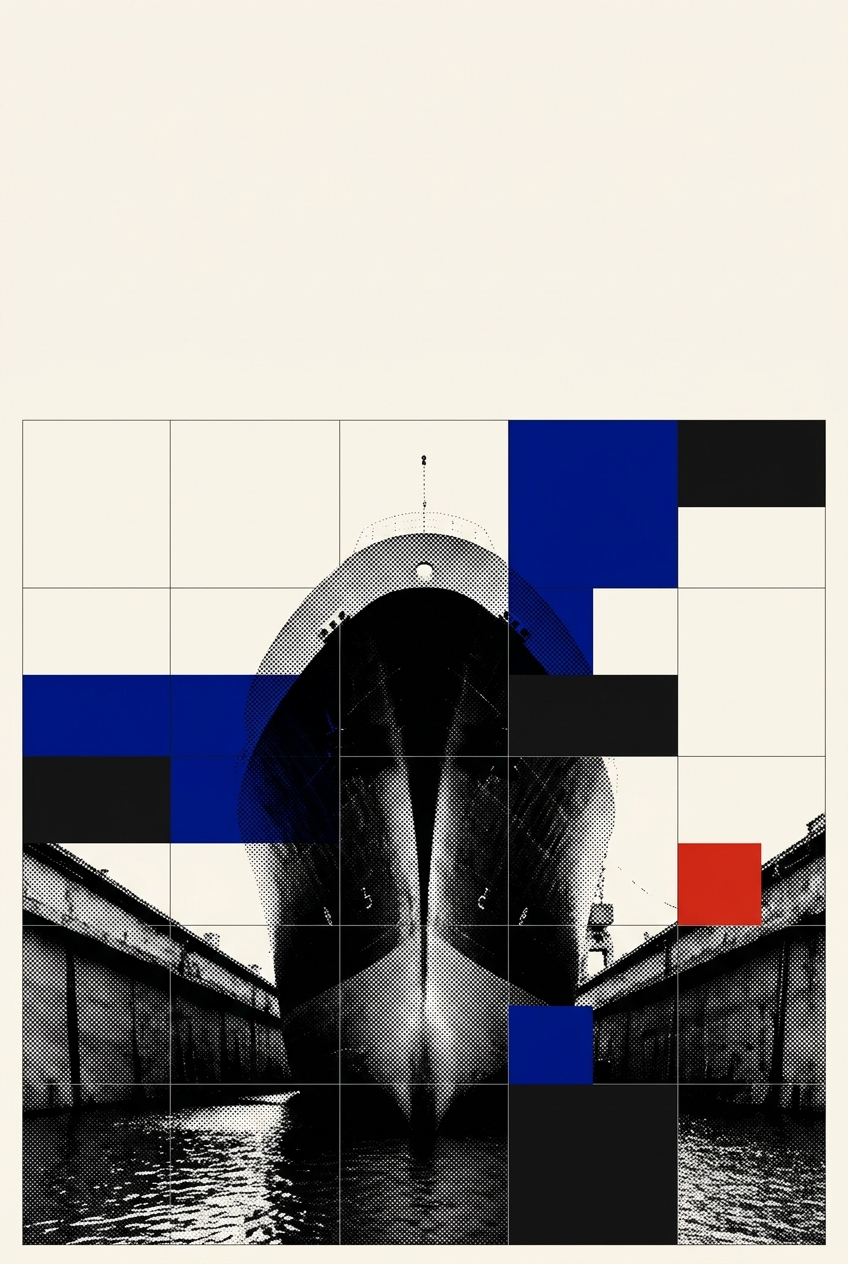
\includegraphics[width=\paperwidth,height=\paperheight]{plates/swiss/cover.jpg}}}}{%
    \PackageError{pd-swiss-plates}{Missing plate render plates/swiss/cover.jpg}{Generate the Swiss cover render and place it at plates/swiss/cover.jpg before building.}}}
\newcommand{\pdswisspartplate}[2]{% #1 numeral I..IV, #2 width
  \IfFileExists{plates/swiss/part-#1.jpg}{%
    \includegraphics[width=#2]{plates/swiss/part-#1.jpg}}{%
    \PackageError{pd-swiss-plates}{Missing plate render plates/swiss/part-#1.jpg}{Generate the Swiss part plate render and place it at plates/swiss/part-#1.jpg before building.}}}
\newcommand{\pdswissplate}[2]{% #1 chapter prefix, #2 width
  \IfFileExists{plates/swiss/chapter-#1.jpg}{%
    \includegraphics[width=#2]{plates/swiss/chapter-#1.jpg}%
  }{%
    \PackageError{pd-swiss-plates}{Missing plate render plates/swiss/chapter-#1.jpg}{Generate the Swiss chapter plate render and place it at plates/swiss/chapter-#1.jpg before building.}%
  }%
}
\newcommand{\pdswissfigplate}[2]{% #1 figure name, #2 width
  \IfFileExists{plates/swiss/#1.jpg}{%
    \includegraphics[width=#2]{plates/swiss/#1.jpg}%
  }{%
    \PackageError{pd-swiss-plates}{Missing figure plate render plates/swiss/#1.jpg}{Generate the Swiss figure plate render and place it at plates/swiss/#1.jpg before building.}%
  }%
}
\providecolor{pdswissred}{HTML}{DA291C}
\providecolor{pdcobalt}{HTML}{001489}
\providecolor{hhink}{HTML}{1B1712}
\providecolor{hhgray}{HTML}{5C5650}

% Canonical Landmark titles and pull-quotes
\expandafter\def\csname pdlandmarktitle@01\endcsname{Agentic Psychosis \& Hallucination Cascade}
\expandafter\def\csname pdlandmarkconcept@01\endcsname{Belief Drift \& Hallucination Cascades}
\expandafter\def\csname pdlandmarkquestion@01\endcsname{Can an unanchored swarm deliberate without spiraling into shared delusion?}
\expandafter\def\csname pdlandmarkquote@01\endcsname{When an unanchored swarm feeds on its own unverified assertions, error does not dissipate; it cascades into conviction. Coordination requires shared physical truth, not mutual agreement on hallucinated state.}

\expandafter\def\csname pdlandmarktitle@02\endcsname{Agentic Continuity \& The Overlapping Strand}
\expandafter\def\csname pdlandmarkconcept@02\endcsname{Substrate Continuity \& Overlapping Strands}
\expandafter\def\csname pdlandmarkquestion@02\endcsname{When every token and worker dies, what actually holds identity across time?}
\expandafter\def\csname pdlandmarkquote@02\endcsname{Identity is not an indivisible core preserved across time, but the continuous overlap of many short fibers. No single thread runs the full length of the rope; the strength is entirely in the friction between the splices.}

\expandafter\def\csname pdlandmarktitle@03\endcsname{The Engine Swap}
\expandafter\def\csname pdlandmarkconcept@03\endcsname{The Engine Swap \& Model Portability}
\expandafter\def\csname pdlandmarkquestion@03\endcsname{Can you replace the brain of a running system while keeping all its commitments intact?}
\expandafter\def\csname pdlandmarkquote@03\endcsname{The intelligence engine may be unbolted and swapped out in mid-voyage. What survives the swap is not the neural weights, but the unbroken hull of contracts, claims, and verified ledger obligations.}

\expandafter\def\csname pdlandmarktitle@04\endcsname{The Front-Loaded Probation Cliff}
\expandafter\def\csname pdlandmarkconcept@04\endcsname{The Front-Loaded Probation Cliff}
\expandafter\def\csname pdlandmarkquestion@04\endcsname{Why should an operating system ever trust an unverified autonomous actor?}
\expandafter\def\csname pdlandmarkquote@04\endcsname{Autonomy is never granted on faith; it is won against a sheer cliff of probation. The newcomer faces strict confinement until its attestation record proves it will not compromise the commons.}

\expandafter\def\csname pdlandmarktitle@05\endcsname{The Single-Writer Monotonic Horizon}
\expandafter\def\csname pdlandmarkconcept@05\endcsname{The Single-Writer Monotonic Horizon}
\expandafter\def\csname pdlandmarkquestion@05\endcsname{How do distributed agents agree on what happened first without Byzantine consensus?}
\expandafter\def\csname pdlandmarkquote@05\endcsname{One writer, one lock, one monotonic frontier. Beyond the commit horizon, the unwritten future remains empty paper; behind it, no write may ever be undone, denied, or reordered.}

\expandafter\def\csname pdlandmarktitle@06\endcsname{The Attenuation Frontier \& Cryptographic Macaroons}
\expandafter\def\csname pdlandmarkconcept@06\endcsname{The Attenuation Frontier \& Macaroons}
\expandafter\def\csname pdlandmarkquestion@06\endcsname{How do permissions travel across machines without accidentally widening?}
\expandafter\def\csname pdlandmarkquote@06\endcsname{Every delegation narrows the aperture of authority. A bearer credential cannot expand its reach as it traverses the network; it can only accumulate cryptographic caveats that bind its hands.}

\expandafter\def\csname pdlandmarktitle@07\endcsname{Attestation Without Revelation (The Sealed Harbor)}
\expandafter\def\csname pdlandmarkconcept@07\endcsname{Attestation Without Revelation (Sealed Harbor)}
\expandafter\def\csname pdlandmarkquestion@07\endcsname{Can a worker prove its computation was correct without revealing what it saw?}
\expandafter\def\csname pdlandmarkquote@07\endcsname{The enclave proves what was computed without disclosing what was seen. Trust in autonomous labor cannot demand total transparency; it demands unforgeable evidence of compliance.}

\expandafter\def\csname pdlandmarktitle@08\endcsname{Read-Poverty \& The Legible Swarm}
\expandafter\def\csname pdlandmarkconcept@08\endcsname{Read-Poverty \& Stigmergic Signaling}
\expandafter\def\csname pdlandmarkquestion@08\endcsname{Why is an agent that reads everything destined to bankrupt its operator?}
\expandafter\def\csname pdlandmarkquote@08\endcsname{In an ocean of synthetic prose, reading is infinitely more expensive than writing. A legible swarm does not shout across channels; it leaves quiet, structured pheromones in the environment.}

\expandafter\def\csname pdlandmarktitle@09\endcsname{Skills as Capital vs.\ Token Labor}
\expandafter\def\csname pdlandmarkconcept@09\endcsname{Skills as Capital vs. Perishable Token Labor}
\expandafter\def\csname pdlandmarkquestion@09\endcsname{When does prompt deliberation become too expensive compared to compiled code?}
\expandafter\def\csname pdlandmarkquote@09\endcsname{Token generation is perishable labor; compiled deterministic tools are durable capital. An economy matures when agents stop paying per token to deliberate and start amortizing proven apparatus.}

\expandafter\def\csname pdlandmarktitle@10\endcsname{The Bonded Commons \& Sacrificial Slashing}
\expandafter\def\csname pdlandmarkconcept@10\endcsname{The Bonded Commons \& Sacrificial Slashing}
\expandafter\def\csname pdlandmarkquestion@10\endcsname{What stops an agent from promising the world and walking away from disaster?}
\expandafter\def\csname pdlandmarkquote@10\endcsname{Trust without collateral is wishful thinking. An agent stakes its bond in the escrow of the commons; when an invariant is breached, the tripwire snaps and the stake is forfeited without appeal.}

\expandafter\def\csname pdlandmarktitle@11\endcsname{Sheaf Laplacian Invariance \& Cycle Consistency}
\expandafter\def\csname pdlandmarkconcept@11\endcsname{Sheaf Laplacians \& Cycle Holonomy}
\expandafter\def\csname pdlandmarkquestion@11\endcsname{Can a network of liars agree locally on every edge while still being caught globally?}
\expandafter\def\csname pdlandmarkquote@11\endcsname{Local consistency along every pairwise edge does not guarantee global truth. When an assertion traverses a closed cycle of harbors and returns altered, the non-zero holonomy reveals the fraud.}

\expandafter\def\csname pdlandmarktitle@12\endcsname{The Zombie Reclaim \& Salvage Graveyard}
\expandafter\def\csname pdlandmarkconcept@12\endcsname{Zombie Salvage \& Dead-Man Leases}
\expandafter\def\csname pdlandmarkquestion@12\endcsname{When an agent crashes in the dark, who buries the body and recovers the locks?}
\expandafter\def\csname pdlandmarkquote@12\endcsname{The graveyard of abandoned sessions is the foundation of harbor resilience. When a heartbeat goes cold, no ghost may linger; the lease expires, the locks are salvaged, and the port is reclaimed.}

% Single-digit alias fallbacks
\expandafter\def\csname pdlandmarktitle@1\endcsname{\csname pdlandmarktitle@01\endcsname}
\expandafter\def\csname pdlandmarkconcept@1\endcsname{\csname pdlandmarkconcept@01\endcsname}
\expandafter\def\csname pdlandmarkquestion@1\endcsname{\csname pdlandmarkquestion@01\endcsname}
\expandafter\def\csname pdlandmarkquote@1\endcsname{\csname pdlandmarkquote@01\endcsname}

\expandafter\def\csname pdlandmarktitle@2\endcsname{\csname pdlandmarktitle@02\endcsname}
\expandafter\def\csname pdlandmarkconcept@2\endcsname{\csname pdlandmarkconcept@02\endcsname}
\expandafter\def\csname pdlandmarkquestion@2\endcsname{\csname pdlandmarkquestion@02\endcsname}
\expandafter\def\csname pdlandmarkquote@2\endcsname{\csname pdlandmarkquote@02\endcsname}

\expandafter\def\csname pdlandmarktitle@3\endcsname{\csname pdlandmarktitle@03\endcsname}
\expandafter\def\csname pdlandmarkconcept@3\endcsname{\csname pdlandmarkconcept@03\endcsname}
\expandafter\def\csname pdlandmarkquestion@3\endcsname{\csname pdlandmarkquestion@03\endcsname}
\expandafter\def\csname pdlandmarkquote@3\endcsname{\csname pdlandmarkquote@03\endcsname}

\expandafter\def\csname pdlandmarktitle@4\endcsname{\csname pdlandmarktitle@04\endcsname}
\expandafter\def\csname pdlandmarkconcept@4\endcsname{\csname pdlandmarkconcept@04\endcsname}
\expandafter\def\csname pdlandmarkquestion@4\endcsname{\csname pdlandmarkquestion@04\endcsname}
\expandafter\def\csname pdlandmarkquote@4\endcsname{\csname pdlandmarkquote@04\endcsname}

\expandafter\def\csname pdlandmarktitle@5\endcsname{\csname pdlandmarktitle@05\endcsname}
\expandafter\def\csname pdlandmarkconcept@5\endcsname{\csname pdlandmarkconcept@05\endcsname}
\expandafter\def\csname pdlandmarkquestion@5\endcsname{\csname pdlandmarkquestion@05\endcsname}
\expandafter\def\csname pdlandmarkquote@5\endcsname{\csname pdlandmarkquote@05\endcsname}

\expandafter\def\csname pdlandmarktitle@6\endcsname{\csname pdlandmarktitle@06\endcsname}
\expandafter\def\csname pdlandmarkconcept@6\endcsname{\csname pdlandmarkconcept@06\endcsname}
\expandafter\def\csname pdlandmarkquestion@6\endcsname{\csname pdlandmarkquestion@06\endcsname}
\expandafter\def\csname pdlandmarkquote@6\endcsname{\csname pdlandmarkquote@06\endcsname}

\expandafter\def\csname pdlandmarktitle@7\endcsname{\csname pdlandmarktitle@07\endcsname}
\expandafter\def\csname pdlandmarkconcept@7\endcsname{\csname pdlandmarkconcept@07\endcsname}
\expandafter\def\csname pdlandmarkquestion@7\endcsname{\csname pdlandmarkquestion@07\endcsname}
\expandafter\def\csname pdlandmarkquote@7\endcsname{\csname pdlandmarkquote@07\endcsname}

\expandafter\def\csname pdlandmarktitle@8\endcsname{\csname pdlandmarktitle@08\endcsname}
\expandafter\def\csname pdlandmarkconcept@8\endcsname{\csname pdlandmarkconcept@08\endcsname}
\expandafter\def\csname pdlandmarkquestion@8\endcsname{\csname pdlandmarkquestion@08\endcsname}
\expandafter\def\csname pdlandmarkquote@8\endcsname{\csname pdlandmarkquote@08\endcsname}

\expandafter\def\csname pdlandmarktitle@9\endcsname{\csname pdlandmarktitle@09\endcsname}
\expandafter\def\csname pdlandmarkconcept@9\endcsname{\csname pdlandmarkconcept@09\endcsname}
\expandafter\def\csname pdlandmarkquestion@9\endcsname{\csname pdlandmarkquestion@09\endcsname}
\expandafter\def\csname pdlandmarkquote@9\endcsname{\csname pdlandmarkquote@09\endcsname}

\newcommand{\pdswisslandmarkplate}[2]{% #1 landmark ID (e.g. 01..12), #2 width
  \IfFileExists{plates/swiss/landmark-#1.jpg}{%
    \centering
    \includegraphics[width=#2]{plates/swiss/landmark-#1.jpg}%
    \par\vspace{10pt}%
    \begin{minipage}{\linewidth}%
      {\color{pdcobalt}\rule{\linewidth}{1.2pt}}\par\vspace{6pt}%
      \raggedright
      {\color{pdswissred}\rule{4.5pt}{4.5pt}}\enspace%
      {\pdgrotesk\bfseries\scshape\fontsize{9}{11}\selectfont\color{hhink}%
        Landmark #1\enspace\textperiodcentered\enspace\csname pdlandmarktitle@#1\endcsname}\par\vspace{4.5pt}%
      {\pdgrotesk\itshape\fontsize{9.5}{13.5}\selectfont\color{hhink}%
        ``\csname pdlandmarkquote@#1\endcsname''\par}%
      \vspace{6pt}%
      {\color{hhgray!30}\rule{\linewidth}{0.4pt}}%
    \end{minipage}%
  }{%
    \PackageError{pd-swiss-plates}{Missing plate render plates/swiss/landmark-#1.jpg}{Generate the Swiss landmark plate render and place it at plates/swiss/landmark-#1.jpg before building.}}}
\makeatother

\fi
% Wordless interstitial art for the Swiss Book, not numbered evidence figures.
% Insert only at an authored paragraph boundary. On verso the plate faces
% following text; on recto it faces preceding text. Never split an arbitrary
% text page, paragraph, worked example, or proof to manufacture verso parity.
\makeatletter
\providecommand{\pdreflectionrecord}[2]{}
\providecommand*{\toclevel@pdplate}{1}
\definecolor{pdreflectionpanel}{HTML}{00564C}
% Interstitials have their own contents entry; they must not advance the
% chapter-art counter used by the illustrated chapter contents.
\newcommand{\pdreflectiontitle}[2]{%
  \expandafter\def\csname pd@reflection@title@#1\endcsname{#2}}
\pdreflectiontitle{the-unseen-boat}{What a summary leaves unseen}
\pdreflectiontitle{the-waiting-body}{What survives the worker}
\pdreflectiontitle{the-paper-crossing}{A commitment between independent shores}
\pdreflectiontitle{the-controlled-opening}{The controlled opening}
% Text-bearing plates declare their own reserved, opaque lower panel.
% Existing wordless plates do not acquire generic captions or title bars.
\newcommand{\pdreflectionbody}[2]{%
  \expandafter\def\csname pd@reflection@body@#1\endcsname{#2}}
\pdreflectionbody{the-controlled-opening}{%
  A closed cabinet still has a slot. A confined agent still has an output.
  The noninterference claim must name what that output may reveal and which
  other channels the model excludes.}
\newcommand{\pdreflectiontocentry}[2]{%
  \begin{minipage}[c]{.19\linewidth}%
    \includegraphics[width=\linewidth,height=.62in,keepaspectratio]{plates/interstitial/#1.png}%
  \end{minipage}\hfill
  \begin{minipage}[c]{.76\linewidth}\raggedright\small
    Plate: #2%
  \end{minipage}}
\newcommand*{\l@pdplate}[2]{%
  \par\addvspace{7pt}\noindent
  \begin{minipage}[c]{.90\linewidth}#1\end{minipage}\hfill
  \makebox[.07\linewidth][r]{\small #2}\par\addvspace{7pt}}
\newcommand{\pd@reflection@render}[1]{%
  \IfFileExists{plates/interstitial/#1.png}{%
    \thispagestyle{empty}%
    \ifcsname pd@reflection@title@#1\endcsname
      \phantomsection\label{plate:#1}%
    \else
      \PackageError{pd-reflection-plates}{Missing contents title for #1}%
        {Register this plate with pdreflectiontitle before placing it.}%
    \fi
    \protected@write\@auxout{}{\string\pdreflectionrecord{#1}{\thepage}}%
    \AddToShipoutPictureBG*{\AtPageCenter{\makebox(0,0){%
      \includegraphics[width=6in,height=9in,keepaspectratio]{plates/interstitial/#1.png}}}}%
    \ifcsname pd@reflection@body@#1\endcsname
      \AddToShipoutPictureFG*{\AtPageCenter{\makebox(0,0){\begingroup
        % Page art is not a column figure. Undo the Book's centering wrapper,
        % as the existing full-page cover renderer does.
        \ifdefined\pd@typesetpicturebox\let\pgfsys@typesetpicturebox\pd@typesetpicturebox\fi
        \begin{tikzpicture}[x=1in,y=1in]
          \useasboundingbox (0,0) rectangle (6,9);
          \fill[pdreflectionpanel] (0,0) rectangle (6,2.45);
          \node[anchor=north west,inner sep=0,text=white,text width=5in,
            font=\fontsize{17}{21}\selectfont\bfseries] at (.5,2.05)
            {\csname pd@reflection@title@#1\endcsname};
          \node[anchor=north west,inner sep=0,text=white,text width=5in,
            font=\fontsize{11}{15}\selectfont,align=left] at (.5,1.5)
            {\raggedright\hyphenpenalty=10000\csname pd@reflection@body@#1\endcsname};
        \end{tikzpicture}\endgroup}}}%
    \fi
    \null\newpage
  }{\PackageError{pd-reflection-plates}{Missing interstitial plate #1}%
    {Restore plates/interstitial/#1.png and its provenance before building.}}%
}
\newcommand{\pd@reflection@place}[1]{%
  \clearpage
  \pd@reflection@render{#1}%
}
\newcommand{\pdreflectionplate}[1]{%
  \ifpdswiss\pd@reflection@place{#1}\fi
}
\makeatother


% The maturity, guarantee, proof-obligation and claim-evidence vocabularies --
% \Built, \BuiltWeak, \Designed, \Vision, their uppercase aliases, \NotGuar,
% \Closed, \Partial, \Open, \SpecOnly, \Verified, \Proved, \Unproved -- and
% \code are defined once, for this volume and for every standalone chapter, in
% figures/pd-pedagogy.tex (\input above).
%
% They used to be listed here AND again in each chapter's own preamble. The
% generator keeps only what lies between \begin{document} and \end{document},
% so the chapter copies never reached this document and the two sets were free
% to disagree -- which they did: chapter 4 printed "built" and "designed" when
% it compiled alone and "implemented" and "specified" at the same call sites
% here. One definition, in a file both preambles read, is what makes a marker
% mean the same thing in both places.
% scripts/harbor-research/check_duplicate_macros.py fails the build if a
% second definition of any of these names comes back.

\newcommand{\pullquote}[1]{%
  \par\vspace{6pt}\noindent\begin{tikzpicture}
  \node[draw=none,fill=hhsand!22,inner sep=10pt,text width=\dimexpr\textwidth-30pt\relax,align=left] (q) {\itshape\large #1};
  \draw[hhcobalt,line width=2.5pt] (q.north west) -- (q.south west);
  \end{tikzpicture}\par\vspace{6pt}}
\newcommand{\keyidea}[1]{%
  \par\vspace{6pt}\noindent\begin{tikzpicture}
  \node[draw=none,fill=hhsand!18,rounded corners=2pt,inner sep=9pt,text width=\dimexpr\textwidth-26pt\relax,align=left] (k)
        {{\scshape\bfseries\color{hhgray}\small Key idea.}\enspace #1};
  \draw[hhgray!60,line width=1pt] (k.north west) -- (k.south west);
  \end{tikzpicture}\par\vspace{6pt}}
\newcommand{\pitfall}[1]{%
  \par\vspace{6pt}\noindent\begin{tikzpicture}
  \node[draw=none,fill=hhsand!18,rounded corners=2pt,inner sep=9pt,text width=\dimexpr\textwidth-26pt\relax,align=left] (p)
        {{\scshape\bfseries\color{hhcobalt}\small Pitfall.}\enspace #1};
  \draw[hhgray!60,line width=1pt] (p.north west) -- (p.south west);
  \end{tikzpicture}\par\vspace{6pt}}
\newcommand{\xrefbox}[1]{%
  \vspace{4pt}\noindent\begin{tikzpicture}
  \node[draw=hhgray!45,line width=0.4pt,fill=hhsand!18,rounded corners=2pt,inner sep=8pt,text width=\dimexpr\textwidth-22pt\relax,align=left]{\small #1};
  \end{tikzpicture}\vspace{4pt}}
\newcommand{\scene}[2]{%
  \par\vspace{8pt plus 2pt}\noindent\begin{tcolorbox}[
    enhanced, breakable, sharp corners,
    colback=white, colframe=black,
    boxrule=0.5pt, leftrule=3.2pt,
    left=9pt, right=9pt, top=7pt, bottom=7pt,
    before skip=6pt, after skip=6pt
  ]%
  \noindent{\small\raisebox{-2pt}{\IfFileExists{figures/icons/mira-silhouette.pdf}{
\includegraphics[height=1.35em]{figures/icons/mira-silhouette.pdf}}{\IfFileExists{figures/icons/mira-silhouette.png}{
\includegraphics[height=1.35em]{figures/icons/mira-silhouette.png}}{}}}\enspace{\scshape\bfseries\color{black}Scene}\enspace\textperiodcentered\enspace{\bfseries #1}\pdblockheadingend{\itshape #2}}%
  \end{tcolorbox}\par\vspace{8pt plus 2pt}}
\newcommand{\openstar}{{\textcolor{hhcobalt}{$\bigstar$}}\;}
\newcommand{\exhead}[1]{\par\vspace{4pt}\noindent{\scshape\bfseries\color{hhink}#1}\par\vspace{-2pt}}

% Chapter-local exercise idioms keep authored semantics under one visual grammar.
\newenvironment{lsexercises}{%
  \par\vspace{8pt}\noindent\begin{tikzpicture}
  \node[draw=hhgray!45,line width=0.4pt,fill=hhsand!12,rounded corners=2pt,inner sep=10pt,text width=\dimexpr\textwidth-28pt\relax,align=left]\bgroup
  \begin{minipage}{\dimexpr\textwidth-30pt\relax}
  {\scshape\bfseries\color{hhink}Exercises}\par\vspace{3pt}\small
}{\end{minipage}\egroup;\end{tikzpicture}\par\vspace{8pt}}
\newenvironment{stpexercises}{%
  \par\vspace{8pt}\noindent\begin{tikzpicture}
  \node[draw=hhgray!45,line width=0.4pt,fill=hhsand!12,rounded corners=2pt,inner sep=10pt,text width=\dimexpr\textwidth-26pt\relax,align=left]\bgroup
  \begin{minipage}{\dimexpr\textwidth-46pt\relax}
  {\scshape\bfseries\color{hhink}\large Exercises}\par\vspace{3pt}\small
}{\end{minipage}\egroup;\end{tikzpicture}\par\vspace{8pt}}
\newenvironment{heexercises}{%
  \par\vspace{8pt}\noindent
  {\scshape\bfseries\textcolor{hhink}{\textcolor{hhgray!70}{\rule[-1pt]{2.5pt}{11pt}}\enspace Exercises}}
  \par\nobreak\vspace{2pt}
  \begin{enumerate}[label=\textbf{E\arabic*.},leftmargin=2.6em,itemsep=2pt,topsep=2pt]
}{\end{enumerate}\vspace{6pt}}
\newcommand{\swkexercises}[1]{%
  \par\vspace{8pt}\noindent\begin{tikzpicture}
  \node[draw=hhgray!45,line width=0.4pt,fill=hhsand!12,rounded corners=2pt,inner sep=9pt,text width=\dimexpr\textwidth-26pt\relax,align=left]
        {{\scshape\bfseries\textcolor{hhink}{Exercises.}}\par\vspace{3pt}#1};
  \end{tikzpicture}\par\vspace{6pt}}

% Code and pseudocode as a printed book sets them: an indented block in a
% dense monospace with tight leading, keywords bold, comments italic grey,
% small grey line numbers, no frame, no background, no stripes. A wrapped
% line continues under a small grey hook.
\lstdefinestyle{pdcode}{language=C,backgroundcolor={},frame=none,
  basicstyle=\ttfamily\fontsize{8.6}{10.6}\selectfont,columns=fullflexible,keepspaces=true,
  keywordstyle=\bfseries,commentstyle=\color{hhgray}\itshape,
  stringstyle=\color{hhink!70!hhgray},numbers=left,numberstyle=\fontsize{6.5}{7}\selectfont\color{hhgray},
  numbersep=7pt,breaklines=true,breakatwhitespace=false,breakindent=1.6em,
  postbreak=\mbox{\textcolor{hhgray}{\fontsize{7}{7}\selectfont$\hookrightarrow$}\space},
  showstringspaces=false,tabsize=2,aboveskip=7pt,belowskip=5pt,
  xleftmargin=1.9em,xrightmargin=0pt,captionpos=b}
\lstdefinestyle{pseudocode}{style=pdcode,
  morekeywords={function,return,if,then,else,for,while,do,begin,end,atomic,transaction,reject,commit,assert,raise}}
\lstdefinestyle{proverif}{style=pdcode}
\lstdefinestyle{rust}{style=pdcode,tabsize=4}
\lstdefinestyle{tlaplus}{style=pdcode,
  morekeywords={MODULE,EXTENDS,CONSTANTS,VARIABLES,VARIABLE,Init,Next,Spec,
  TypeOK,IF,THEN,ELSE,LET,IN,CHOOSE,SUBSET,UNION,DOMAIN,EXCEPT,
  UNCHANGED,TRUE,FALSE,BOOLEAN,Nat,Int,STRING,Seq,Append,Len,Head,Tail,
  ENABLED,WF_,SF_,THEOREM,ASSUME,INSTANCE,WITH,LOCAL}}
\lstset{style=pdcode}

% Shared presentation primitives, loaded without adopting the broader semantic
% or margin-layout changes. Only protocols opt into the frame and glyph here.
% Presentation only. Official Lucide assets: figures/lucide/LICENSE.
\makeatletter
\definecolor{pdblockProof}{HTML}{B33F35}
\definecolor{pdblockProperty}{HTML}{7048A5}
\definecolor{pdblockHypothesis}{HTML}{427A26}
\definecolor{pdblockCalculation}{HTML}{946000}
\definecolor{pdblockInvariant}{HTML}{233A76}
\definecolor{pdblockDefinition}{HTML}{3D454B}
\definecolor{pdblockChecked}{HTML}{006EA0}
\definecolor{pdblockProtocol}{HTML}{007D73}
\definecolor{pdblockNeutral}{HTML}{363B40}
\ifdefined\pdblockfamily\else
\newcommand{\pdblockfamily}[1]{%
  \def\pdblock@family{#1}%
  \ifdefstring{\pdblock@family}{Conjecture}{\def\pdblock@family{Empirical hypothesis}}{}%
  \def\pdblock@color{pdblockNeutral}\def\pdblock@icon{file-text}%
  \ifdefstring{\pdblock@family}{Theorem}{\def\pdblock@color{pdblockProof}\def\pdblock@icon{scroll-text}}{}%
  \ifdefstring{\pdblock@family}{Lemma}{\def\pdblock@color{pdblockProof}\def\pdblock@icon{scroll-text}}{}%
  \ifdefstring{\pdblock@family}{Proposition}{\def\pdblock@color{pdblockProof}\def\pdblock@icon{scroll-text}}{}%
  \ifdefstring{\pdblock@family}{Corollary}{\def\pdblock@color{pdblockProof}\def\pdblock@icon{scroll-text}}{}%
  \ifdefstring{\pdblock@family}{Property}{\def\pdblock@color{pdblockProperty}\def\pdblock@icon{key-round}}{}%
  \ifdefstring{\pdblock@family}{Definition}{\def\pdblock@color{pdblockDefinition}\def\pdblock@icon{book-open}}{}%
  \ifdefstring{\pdblock@family}{Empirical hypothesis}{\def\pdblock@color{pdblockHypothesis}\def\pdblock@icon{flask-conical}}{}%
  \ifdefstring{\pdblock@family}{Numbers by hand}{\def\pdblock@color{pdblockCalculation}\def\pdblock@icon{calculator}}{}%
  \ifdefstring{\pdblock@family}{Design invariant}{\def\pdblock@color{pdblockInvariant}\def\pdblock@icon{lock-keyhole}}{}%
  \ifdefstring{\pdblock@family}{Model-checked property}{\def\pdblock@color{pdblockChecked}\def\pdblock@icon{list-checks}}{}%
  \ifdefstring{\pdblock@family}{Protocol}{\def\pdblock@color{pdblockProtocol}\def\pdblock@icon{workflow}}{}%
}
\fi
\providecommand{\pdblock@inlinebegin}{%
  \ifcsname pd@typesetpicturebox\endcsname
    \let\pgfsys@typesetpicturebox\pd@typesetpicturebox
  \fi}
\providecommand{\pdblockglyph}[1]{\begingroup
  \edef\pdblock@expanded{#1}\expandafter\pdblockfamily\expandafter{\pdblock@expanded}%
  \raisebox{-2.2pt}{\includegraphics[width=12pt,height=12pt]{figures/lucide/\pdblock@icon.pdf}}%
  \endgroup\hspace{.45em}}
% Every split segment keeps a full-strength 0.5pt perimeter for the Book inks.
% The retained 2% field and corner geometry are specific to this protocol slice.
% The colored upper-left cap
% is longer than its upright; the lower-right upright is longer than its cap.
\providecommand{\pdblock@frame}{%
  \draw[draw=\pdblock@color,line width=.5pt]
    (frame.south west) rectangle (frame.north east);
  \fill[\pdblock@color] (frame.north west) rectangle
    ([xshift=32pt,yshift=-3pt]frame.north west);
  \fill[\pdblock@color] (frame.north west) rectangle
    ([xshift=3pt,yshift=-16pt]frame.north west);
  \fill[\pdblock@color] (frame.south east) rectangle
    ([xshift=-16pt,yshift=3pt]frame.south east);
  \fill[\pdblock@color] (frame.south east) rectangle
    ([xshift=-3pt,yshift=28pt]frame.south east);}
\providecommand{\pdblockbefore}[1]{%
  \par\if@nobreak\else\Needspace{5\baselineskip}\fi
  \begingroup
  \edef\pdblock@expanded{#1}\expandafter\pdblockfamily\expandafter{\pdblock@expanded}%
  \pdblock@inlinebegin
  \begin{tcolorbox}[enhanced,breakable,sharp corners,frame hidden,
    colback=\pdblock@color!2!white,boxrule=.45pt,boxsep=0pt,
    left=8pt,right=8pt,top=7pt,bottom=7pt,
    before skip=8pt plus 2pt,after skip=8pt plus 2pt,
    pad at break*=7pt,lines before break=6,
    overlay unbroken={\pdblock@frame},overlay first={\pdblock@frame},
    overlay middle={\pdblock@frame},overlay last={\pdblock@frame}]
    \clubpenalty=9000 \widowpenalty=9000
    \displaywidowpenalty=9000 \brokenpenalty=9000
}
\providecommand{\pdblockafter}[1]{\par\end{tcolorbox}\endgroup}
\makeatother


% Fixed, restrained theorem skips keep theorem/prose transitions on the same
% baseline cadence. A block heading is separate from its first body paragraph.
% amsthm's class defaults carry highly stretchable vertical
% glue, which produced visibly unrelated gaps at page breaks in chapter 7.
\newtheoremstyle{pddefinition}% name
  {7pt plus 1pt minus 1pt}{7pt plus 1pt minus 1pt}% above / below
  {\normalfont}{}% body / indent
  {\bfseries}{.}{0pt}{\pdblockglyph{#1}\thmname{#1}\thmnumber{\ #2}\thmnote{\hspace{.35em}(#3)}}% head
\newtheoremstyle{pdplain}% name
  {7pt plus 1pt minus 1pt}{7pt plus 1pt minus 1pt}% above / below
  {\itshape}{}% body / indent
  {\bfseries}{.}{0pt}{\pdblockglyph{#1}\thmname{#1}\thmnumber{\ #2}\thmnote{\hspace{.35em}(#3)}}% head
\newtheoremstyle{pdremark}% name
  {6pt plus 1pt minus 1pt}{6pt plus 1pt minus 1pt}% above / below
  {\normalfont}{}% body / indent
  {\itshape}{.}{0pt}{\pdblockglyph{#1}\thmname{#1}\thmnumber{\ #2}\thmnote{\hspace{.35em}(#3)}}% head

\newtheoremstyle{pdprotocol}
  {7pt plus 1pt minus 1pt}{7pt plus 1pt minus 1pt}
  {\normalfont}{}{\bfseries}{.}{0pt}
  {\pdblockglyph{Protocol}\thmname{#1}\thmnumber{\ #2}\thmnote{\hspace{.35em}(#3)}}
\makeatletter
\newcommand{\pdprotocolheadingend}{%
  \par\nobreak\smallskip\@afterindentfalse\@afterheading\ignorespaces}
% AtBeginEnvironment runs inside the environment group, before amsthm builds
% its deferred heading. Flush that heading, then end its paragraph even when
% the body begins with a list. Preserve nameref's wrapper and restore the entry
% and heading renderer immediately, so nested unrelated families are unchanged.
\newcommand{\pdprotocolparagraphs}{%
  \let\pdprotocolsavedentry\@begintheorem
  \let\pdprotocolsavedhead\thmhead
  \apptocmd{\@begintheorem}{\leavevmode\pdprotocolheadingend
    \let\@begintheorem\pdprotocolsavedentry
    \let\thmhead\pdprotocolsavedhead\ignorespaces}{}%
    {\PackageError{pdprotocol}{Cannot terminate the protocol heading}{Check the amsthm entry point.}}}
\AtBeginEnvironment{protocol}{\pdprotocolparagraphs}
\AtBeginEnvironment{heprotocol}{\pdprotocolparagraphs}
\makeatother

\theoremstyle{definition}
\newtheorem{definition}{Definition}[section]
\newtheorem{property}{Property}[section]
\theoremstyle{pdprotocol}
\newtheorem{protocol}{Protocol}[section]
\theoremstyle{plain}
\newtheorem{theorem}{Theorem}[section]
\newtheorem{lemma}{Lemma}[section]
\newtheorem{proposition}{Proposition}[section]
\newtheorem{corollary}{Corollary}[section]
\newtheorem{conjecture}{Conjecture}[section]
\theoremstyle{remark}
\newtheorem*{remark}{Remark}
% Flush amsthm's deferred label into its own paragraph before body tokens.
% A head-separator newline alone leaves an opening list's marker on the head.
\makeatletter
\patchcmd{\@begintheorem}{\ignorespaces}{\leavevmode\pdblockheadingend}{}%
  {\PackageError{pd-book}{Theorem heading paragraph patch failed}{Check the amsthm heading definition.}}
\makeatother
% Keep the usual proof/QED machinery, but separate the proof heading too.
\expandafter\patchcmd\csname\string\proof\endcsname
  {\ignorespaces}{\leavevmode\pdblockheadingend}{}%
  {\PackageError{pd-book}{Proof heading paragraph patch failed}{Check the amsthm proof definition.}}
\BeforeBeginEnvironment{protocol}{\pdblockbefore{Protocol}}
\AfterEndEnvironment{protocol}{\pdblockafter{Protocol}}


\newcounter{lsprotocol}[section]
\renewcommand{\thelsprotocol}{\thesection.\arabic{lsprotocol}}
% Protocol prose is not a drawing: a TikZ/minipage wrapper made the whole
% passage indivisible and left half-pages empty. Both chapter variants now
% share one breakable frame while keeping their counters and labels intact.
\newenvironment{pdbookprotocol}[2]{%
  \pdblockbefore{Protocol}%
  % The destination belongs inside the frame, after its start reservation.
  \refstepcounter{#1}%
  \noindent{\raggedright\normalfont\bfseries\color{hhink}\pdblockglyph{Protocol}%
    Protocol~\csname the#1\endcsname\ifblank{#2}{}{\hspace{.35em}(#2)}.\par}%
  \small\pdprotocolheadingend
}{\pdblockafter{Protocol}}
\newenvironment{lsprotocol}[1]{%
  \begin{pdbookprotocol}{lsprotocol}{#1}%
}{\end{pdbookprotocol}}
\newcounter{stpprotocol}[section]
\renewcommand{\thestpprotocol}{\thesection.\arabic{stpprotocol}}
\newenvironment{stpprotocol}[1][]{%
  \begin{pdbookprotocol}{stpprotocol}{#1}%
}{\end{pdbookprotocol}}
\theoremstyle{pdprotocol}
\newtheorem{heprotocol}{Protocol}[section]
\BeforeBeginEnvironment{heprotocol}{\pdblockbefore{Protocol}}
\AfterEndEnvironment{heprotocol}{\pdblockafter{Protocol}}
\theoremstyle{definition}

\tikzset{
  stp box/.style={draw=hhink,line width=0.55pt,fill=hhsand!22,rounded corners=2pt,inner sep=7pt,align=center,minimum height=10mm},
  stp accent box/.style={stp box,draw=hhcobalt,line width=0.9pt},
  stp arrow/.style={-{Stealth[length=2.3mm,width=1.5mm]},draw=hhink,line width=0.65pt},
  stp accent arrow/.style={-{Stealth[length=2.3mm,width=1.5mm]},draw=hhcobalt,line width=0.8pt},
  stp dashed arrow/.style={stp accent arrow,dashed},
  stp label/.style={fill=hhpaper,inner xsep=3pt,inner ysep=1.5pt,font=\footnotesize\itshape,text=hhgray},
  stp heading/.style={font=\footnotesize\bfseries,text=hhink},
  stp status/.style={font=\scriptsize\scshape,text=hhgray},
}

\pagestyle{fancy}
\fancyhf{}
\fancyhead[RE,LO]{\small\itshape\color{hhgray} \pdshorttitle}
\fancyhead[LE,RO]{\small\color{hhgray}\thepage}
\fancyfoot[C]{\footnotesize\color{hhgray} Textbook Edition \textperiodcentered\ \pdeditiondate}
\renewcommand{\headrulewidth}{0.4pt}
\renewcommand{\footrulewidth}{0pt}
% Backmatter replaces all chapter heads on both sides of the spread.
\newcommand{\pdbackmatterheaders}[1]{%
  \fancyhead{}%
  \fancyhead[LE,RO]{\small\color{hhgray}\thepage}%
  \fancyhead[RE,LO]{\small\itshape\color{hhgray} #1}%
  \fancyfoot[C]{\footnotesize\color{hhgray}\pdeditiontitle\ \textperiodcentered\ #1}}

% ---- Chapters, parts, and the front-matter map ----------------------------
% Chapter numbers are Arabic and come from whitepaper/textbook.json via the
% generator: \pdchapter{number}{title}{prefix}{hue}. The prefix selects the
% chapter's seam rails and its entry in figures/pd-textbook-map.tex (question,
% epigraph, one-breath answer, part label); the hue is the PART's, inherited by
% every chapter in it, so each part owns one color and nothing dilutes it.
\newcounter{pdchapter}
\renewcommand{\thepdchapter}{\arabic{pdchapter}}
\makeatletter
\@namedef{theHpdchapter}{chap.\arabic{pdchapter}}
\makeatother
\newcommand{\pdcurrentchapter}{0}
\newcommand{\pdcurrentchaptercolor}{pdcobalt}
% A live link to a chapter, by prefix. figures/pd-hyperlinks.tex provides the
% plain-text fallback for standalone chapters; the Book defines the real thing.
\DeclareRobustCommand{\pdchaplink}[2]{\hyperref[chap:#1]{#2}}

% Begin the next material on a verso so a two-page construction is a physical
% facing spread. \cleardoublepage does the opposite: it begins on a recto.
\newcommand{\cleartoleftpage}{%
  \clearpage
  \ifodd\value{page}\thispagestyle{empty}\null\newpage\fi}

% The weighted four-hue rule. One segment per part, its length proportional to
% the part's share of the book's pages (from the page references once they
% exist; chapter counts on the first pass). Segments up to the current part are
% solid, the rest outlined, so the same rule reads as a progress mark on part
% and chapter openers and as the whole book on the title page.
%   \pdweightrule[color]{current part index or 0 for all}{total width}{height}
\newdimen\pdweightx
\newdimen\pdweightw
\newcount\pdweighti
\makeatletter
\newcommand{\pdweightrule}[4][]{%
  \begingroup
  \edef\pd@tot{\the\numexpr\getpagerefnumber{book:appendices}-\getpagerefnumber{part:\pdfirstpartnumeral}\relax}%
  \ifnum\pd@tot<1 \def\pd@tot{0}\fi
  \pdweightx=0pt \pdweighti=0
  \def\pdweightsegment##1##2##3##4{%
    \advance\pdweighti by 1
    \ifnum\pd@tot>0
      \edef\pd@seg{\the\numexpr\getpagerefnumber{##3}-\getpagerefnumber{part:##1}\relax}%
      \ifnum\pd@seg<1 \edef\pd@seg{##4}\edef\pd@den{\pdchaptercount}\else\edef\pd@den{\pd@tot}\fi
    \else
      \edef\pd@seg{##4}\edef\pd@den{\pdchaptercount}%
    \fi
    \pdweightw=\dimexpr(#3-3pt*(\pdpartcount-1))*\pd@seg/\pd@den\relax
    \if\relax\detokenize{#1}\relax\def\pd@col{##2}\else\def\pd@col{#1}\fi
    \ifnum#2=0 \def\pd@solid{1}\else\ifnum\pdweighti>#2 \def\pd@solid{0}\else\def\pd@solid{1}\fi\fi
    \if1\pd@solid
      \fill[color=\pd@col] (\the\pdweightx,0pt) rectangle ++(\the\pdweightw,#4);
    \else
      \draw[color=\pd@col,line width=0.5pt] (\the\dimexpr\pdweightx+0.25pt\relax,0.25pt) rectangle ++(\the\dimexpr\pdweightw-0.5pt\relax,\the\dimexpr#4-0.5pt\relax);
    \fi
    \advance\pdweightx by \pdweightw \advance\pdweightx by 3pt
  }%
  \begin{tikzpicture}[baseline=0pt]
    \pdweightsegmentslist
  \end{tikzpicture}%
  \endgroup}
\makeatother

% The chapter opener: one page with the title, an epigraph, a plate when the
% chapter has one, and the question the chapter answers with its one-breath
% answer. Nothing else. The chapter's first section starts on the next page.
\makeatletter
\def\pd@chapter@maritime#1#2#3#4{%
  \vspace*{0.1cm}
  \noindent{\scshape\footnotesize\color{hhgray}\ifnum#1=0 Chapter 0\hfill\pdchapterpartlabel\else Chapter #1 of \pdchaptercount\hfill\pdchapterpartlabel\fi}\par
  \vspace{0.25cm}
  \noindent\pdweightrule{\pdchapterpartindex}{\textwidth}{2pt}\par
  % The gilt fillet: the trim line of the engraved plates, carried onto the
  % page. Hairline, under the weight rule, and nowhere else on the spread.
  \vspace{2.6pt}\noindent{\color{pdmaritimegold}\rule{\textwidth}{0.4pt}}\par
  \vspace{\dimexpr1.3cm-3pt\relax}
  {\noindent\fontsize{34}{40}\selectfont\color{hhink}\hyphenpenalty=10000\exhyphenpenalty=10000\raggedright #2\par}
  \vspace{1.0cm}
  \begin{flushright}
    \begin{minipage}{0.84\textwidth}\raggedleft
      {\itshape\pdchapterepigraph\par}
      \vspace{5pt}
      {\footnotesize\scshape\color{hhgray}\pdchapterepigraphsource\par}
    \end{minipage}
  \end{flushright}
  % The question block is measured first, then the plate takes what the page
  % still has above it (capped at 0.42 of the text height), and the question
  % closes the page as in the first printing. Nothing can spill: the plate is
  % cut to fit and dropped below 3 cm.
  \sbox{\pdqbox}{\begin{minipage}{\textwidth}
    \noindent{\scshape\footnotesize\color{hhgray}The question this chapter answers}\par
    \vspace{6pt}
    {\noindent\fontsize{21}{26}\selectfont\color{hhink}\hyphenpenalty=10000\exhyphenpenalty=10000\raggedright\pdchapterquestion\par}
    \vspace{9pt}
    {\noindent\small\itshape\pdchapteroneline\par}
  \end{minipage}}%
  \par
  \IfFileExists{plates/chapter-#3.jpg}{%
    \ifdim\pagegoal=\maxdimen
      \setlength{\pdplateh}{\dimexpr\textheight-\pagetotal\relax}%
    \else
      \setlength{\pdplateh}{\dimexpr\pagegoal-\pagetotal\relax}%
    \fi
    \addtolength{\pdplateh}{-\ht\pdqbox}\addtolength{\pdplateh}{-\dp\pdqbox}\addtolength{\pdplateh}{-1.6cm}%
    \ifdim\pdplateh>0.42\textheight \setlength{\pdplateh}{0.42\textheight}\fi
    \ifdim\pdplateh>3cm
      \vspace{0.5cm}%
      \noindent\makebox[\textwidth]{\includegraphics[width=\textwidth,height=\pdplateh,keepaspectratio]{plates/chapter-#3.jpg}}\par
    \fi}{}%
  \vfill
  \noindent\usebox{\pdqbox}\par
  \vspace{0.2cm}
}
% swiss: a colour band carries number and title; the question sits on paper
\def\pd@chapter@swiss#1#2#3#4{%
  \begin{adjustwidth*}{0pt}{-\dimexpr\marginparsep+\marginparwidth\relax}
  \vspace*{-0.5cm}
  \noindent\begin{tikzpicture}
    \node[fill=#4,inner sep=0pt,minimum width=\linewidth,minimum height=0.36\textheight,anchor=north west] (band) at (0,0) {};
    \node[anchor=north west,text=hhpaper,font=\pdgrotesk\fontsize{9.5}{12}\selectfont\bfseries,inner sep=0pt]
      at (0.45cm,-0.5cm) {\ifnum#1=0 Chapter 0\quad\textperiodcentered\quad\pdchapterpartlabel\else Chapter #1 of \pdchaptercount\quad\textperiodcentered\quad\pdchapterpartlabel\fi};
    \node[anchor=south west,text=hhpaper,font=\pddisplayface\fontsize{78}{78}\selectfont\bfseries,inner sep=0pt]
      at (0.4cm,{-0.36\textheight+3.0cm}) {#1};
    \node[anchor=south west,text=hhpaper,font=\pddisplayface\fontsize{27}{31}\selectfont\bfseries,inner sep=0pt,
      text width={\dimexpr\linewidth-1cm\relax},align=left] at (0.45cm,{-0.36\textheight+0.55cm}) {#2};
  \end{tikzpicture}\par
  \vspace{1.0cm}
  \noindent{\pdgrotesk\footnotesize\bfseries\color{hhgray}The question this chapter answers}\par
  \vspace{6pt}
  {\noindent\fontsize{21}{26}\selectfont\color{hhink}\hyphenpenalty=10000\exhyphenpenalty=10000\raggedright\pdchapterquestion\par}
  \vspace{9pt}
  {\noindent\small\itshape\pdchapteroneline\par}
  % Reserve the actual epigraph before choosing the art's height. A fixed
  % plate size let a longer question push the quote onto the next
  % page, where the still-open full-width list also used the wrong parity.
  % Only the raster art scales; the title, question and quote keep their type.
  \sbox{\pdepigraphbox}{\begin{minipage}{0.84\linewidth}\raggedleft
      {\itshape\pdchapterepigraph\par}
      \vspace{5pt}
      {\pdgrotesk\footnotesize\color{hhgray}\pdchapterepigraphsource\par}
    \end{minipage}}%
  \par\vspace{0.55cm}
  \ifdim\pagegoal=\maxdimen
    \setlength{\pdplateh}{\dimexpr\textheight-\pagetotal\relax}%
  \else
    \setlength{\pdplateh}{\dimexpr\pagegoal-\pagetotal\relax}%
  \fi
  \addtolength{\pdplateh}{-\ht\pdepigraphbox}%
  \addtolength{\pdplateh}{-\dp\pdepigraphbox}%
  \addtolength{\pdplateh}{-1.0cm}%
  \addtolength{\pdplateh}{-2\baselineskip}%
  \sbox{\pdopenerplatebox}{\pdswissplate{#3}{0.7\linewidth}}%
  \ifdim\pdplateh<2cm
    \PackageError{pd-book}{Chapter #1 opener has no room for its plate}%
      {Shorten the opener or adjust the shared layout; do not shrink its text.}%
  \fi
  \noindent\ifdim\dimexpr\ht\pdopenerplatebox+\dp\pdopenerplatebox\relax>\pdplateh
    \resizebox*{!}{\pdplateh}{\usebox{\pdopenerplatebox}}%
  \else\usebox{\pdopenerplatebox}\fi\par
  \nobreak\vspace{0.35cm}\vfill
  \noindent\hfill\usebox{\pdepigraphbox}\par
  \vspace{0.3cm}
  \end{adjustwidth*}}
% technical: a drawing sheet; the chapter numeral in the accent, the title
% block at the foot
\def\pd@chapter@technical#1#2#3#4{%
  \pd@techsheet{#2}{Chapter #1}%
  \begin{adjustwidth*}{0pt}{-1.0in}
  \vspace*{0.5cm}
  \noindent{\pdgrotesk\footnotesize \ifnum#1=0 Chapter 0\hfill\pdchapterpartlabel\else Chapter #1 of \pdchaptercount\hfill\pdchapterpartlabel\fi}\par
  \vspace{0.3cm}\noindent{\color{hhink}\rule{\linewidth}{0.5pt}}\par
  \vspace{0.9cm}
  \noindent{\pdgrotesk\fontsize{60}{60}\selectfont\color{pdamber}#1\par}
  \vspace{0.2cm}
  \noindent{\pdgrotesk\fontsize{26}{31}\selectfont\hyphenpenalty=10000\exhyphenpenalty=10000\raggedright #2\par}
  \vspace{0.3cm}
  \begin{flushright}
    \begin{minipage}{0.84\linewidth}\raggedleft
      {\itshape\pdchapterepigraph\par}
      \vspace{5pt}
      {\pdgrotesk\footnotesize\color{hhgray}\pdchapterepigraphsource\par}
    \end{minipage}
  \end{flushright}
  % The question block is measured first; the plate takes what the page still
  % has above it, less the 1.6 cm the title block occupies at the sheet's foot.
  \sbox{\pdqbox}{\begin{minipage}{\linewidth}
    \noindent{\pdgrotesk\footnotesize\bfseries\color{hhgray}The question this chapter answers}\par
    \vspace{6pt}
    {\noindent\fontsize{20}{25}\selectfont\color{hhink}\hyphenpenalty=10000\exhyphenpenalty=10000\raggedright\pdchapterquestion\par}
    \vspace{6pt}
    {\noindent\small\itshape\pdchapteroneline\par}
  \end{minipage}}%
  \par
  \IfFileExists{plates/technical/chapter-#1.jpg}{%
    \ifdim\pagegoal=\maxdimen\setlength{\pdplateh}{\dimexpr\textheight-\pagetotal\relax}\else\setlength{\pdplateh}{\dimexpr\pagegoal-\pagetotal\relax}\fi
    \addtolength{\pdplateh}{-\ht\pdqbox}\addtolength{\pdplateh}{-\dp\pdqbox}\addtolength{\pdplateh}{-3.0cm}%
    \ifdim\pdplateh>0.36\textheight \setlength{\pdplateh}{0.36\textheight}\fi
    \ifdim\pdplateh>3cm
      \vspace{0.35cm}\noindent\makebox[\linewidth][c]{\includegraphics[width=\linewidth,height=\pdplateh,keepaspectratio]{plates/technical/chapter-#1.jpg}}\par
    \fi}{}%
  \vfill
  \noindent\usebox{\pdqbox}\par
  \vspace*{1.6cm}
  \end{adjustwidth*}}
\makeatother
\newsavebox{\pdqbox}\newsavebox{\pdpartbox}\newlength{\pdplateh}
\newsavebox{\pdepigraphbox}\newsavebox{\pdopenerplatebox}
\makeatletter
\newcommand{\pdchapter}[4]{%
  \clearpage
  \renewcommand{\pdcurrentchapter}{#1}%
  \renewcommand{\pdchapterprefix}{#3}%
  \renewcommand{\pdcurrentchaptercolor}{#4}%
  \setcounter{pdchapter}{#1}\addtocounter{pdchapter}{-1}\refstepcounter{pdchapter}%
  \label{chap:#3}%
  \addcontentsline{toc}{chapter}{\protect\numberline{#1}#2}%
  \thispagestyle{empty}%
  \ifpdswiss\pd@chapter@swiss{#1}{#2}{#3}{#4}\else
  \ifpdtechnical\pd@chapter@technical{#1}{#2}{#3}{#4}\else
  \pd@chapter@maritime{#1}{#2}{#3}{#4}\fi\fi
  \clearpage
  \setcounter{section}{0}\setcounter{figure}{0}\setcounter{table}{0}\setcounter{equation}{0}\setcounter{lstlisting}{0}\setcounter{pdexercise}{0}%
  \renewcommand{\thesection}{#1.\arabic{section}}%
  \renewcommand{\thefigure}{#1.\arabic{figure}}%
  \renewcommand{\thetable}{#1.\arabic{table}}%
  \renewcommand{\theequation}{#1.\arabic{equation}}%
  \renewcommand{\thelstlisting}{#1.\arabic{lstlisting}}%
  \renewcommand{\theHsection}{#1.\arabic{section}}%
  \renewcommand{\theHsubsection}{#1.\arabic{section}.\arabic{subsection}}%
  \renewcommand{\theHsubsubsection}{#1.\arabic{section}.\arabic{subsection}.\arabic{subsubsection}}%
  \renewcommand{\theHfigure}{#1.\arabic{figure}}%
  \renewcommand{\theHtable}{#1.\arabic{table}}%
  \renewcommand{\theHequation}{#1.\arabic{equation}}%
  \renewcommand{\theHlstlisting}{#1.\arabic{lstlisting}}%
  \fancyhead[RE,LO]{\small\itshape\color{hhgray} Chapter #1. #2}%
  \fancyfoot[C]{\footnotesize\color{hhgray} \pdeditiontitle\ \textperiodcentered\ \ifnum#1=0 Chapter 0\else Chapter #1 of \pdchaptercount\fi}%
}
\makeatother
\newcommand{\pdchapterappendix}{%
  \clearpage\setcounter{section}{0}%
  \renewcommand{\thesection}{\pdcurrentchapter.\Alph{section}}%
  \renewcommand{\theHsection}{\pdcurrentchapter.appendix.\arabic{section}}%
  \renewcommand{\theHsubsection}{\pdcurrentchapter.appendix.\arabic{section}.\arabic{subsection}}%
  \renewcommand{\theHsubsubsection}{\pdcurrentchapter.appendix.\arabic{section}.\arabic{subsection}.\arabic{subsubsection}}%
  \renewcommand{\theHfigure}{\pdcurrentchapter.appendix.\arabic{figure}}%
  \renewcommand{\theHtable}{\pdcurrentchapter.appendix.\arabic{table}}%
  \renewcommand{\theHequation}{\pdcurrentchapter.appendix.\arabic{equation}}%
  \renewcommand{\theHlstlisting}{\pdcurrentchapter.appendix.\arabic{lstlisting}}%
  \section*{Chapter Appendices}%
  \addcontentsline{toc}{section}{\pdcurrentchapter.\quad Chapter Appendices}}

% Part opener: one full-bleed page in the part's hue, cream text, the part's
% claim, its chapters, and a plate when the part has one.
% \pdpart{numeral}{title}{hue}{blurb}{chapter list}.
% The Swiss and technical part pages spend their height on the numeral, so
% their chapter list is set compact; otherwise a three-chapter part spills the
% list onto a second page that carries the body's running head.
\newif\ifpdcompactpartlist
\newcommand{\pdpartchapter}[4]{%
  \ifpdcompactpartlist
    \par\noindent\pdchaplink{#2}{{\large\bfseries #1}\quad{\bfseries #3}}\par
    \vspace{1pt}\noindent\hspace*{2.0em}\begin{minipage}{0.86\linewidth}\footnotesize #4\end{minipage}\par
    \vspace{5pt}%
  \else
    \par\noindent\pdchaplink{#2}{{\Large\bfseries #1}\quad{\large\bfseries #3}}\par
    \vspace{2pt}\noindent\hspace*{2.4em}\begin{minipage}{0.82\textwidth}\small #4\end{minipage}\par
    \vspace{9pt}%
  \fi}
\makeatletter
% The drawing sheet of the technical edition: frame, inch ticks, faint grid,
% title block bottom right. #1 title, #2 sheet name.
\def\pd@techsheet{\pd@techsheet@{\draw[hhgray!18,line width=.3pt,step=0.5] (0.5,0.5) grid (6.5,9.5);}}
\def\pd@techsheetplain{\pd@techsheet@{}}
\newcommand{\pdtechsheetplain}[2]{\pd@techsheetplain{#1}{#2}}
% #1 the grid command or nothing, #2 title, #3 sheet name
\def\pd@techsheet@#1#2#3{%
  % The overflow safety net must not touch a page background: it would scale
  % the sheet to the column width. It is switched off for this picture only.
  \AddToShipoutPictureBG*{\AtPageLowerLeft{\begingroup\let\pgfsys@typesetpicturebox\pd@typesetpicturebox\begin{tikzpicture}[x=1in,y=1in]
    % The picture is placed by its bounding box, so without this the sheet's
    % (0.5,0.5) corner landed on the page corner and the whole frame sat half
    % an inch low and left, cutting through the running head and epigraphs.
    \useasboundingbox (0,0) rectangle (\paperwidth,\paperheight);
    #1
    \draw[hhink,line width=.7pt] (0.5,0.5) rectangle (6.5,9.5);
    \foreach \x in {1,...,6} \draw[hhink,line width=.5pt] (\x,0.5)--(\x,0.6) (\x,9.4)--(\x,9.5);
    \foreach \y in {1,...,9} \draw[hhink,line width=.5pt] (0.5,\y)--(0.6,\y) (6.4,\y)--(6.5,\y);
    \fill[hhpaper] (2.9,0.5) rectangle (6.5,1.45);
    \draw[hhink,line width=.6pt] (2.9,0.5) rectangle (6.5,1.45);
    \draw[hhink,line width=.4pt] (2.9,0.98)--(6.5,0.98) (4.9,0.5)--(4.9,1.45) (5.9,0.5)--(5.9,1.45);
    \node[anchor=north west,font=\pdgrotesk\fontsize{5.5}{6}\selectfont,text=hhgray,inner sep=2pt] at (2.9,1.45) {TITLE};
    \node[anchor=south west,font=\pdgrotesk\footnotesize,text=hhink,text width=1.9in,align=left,inner sep=3pt] at (2.9,0.98) {#2};
    \node[anchor=north west,font=\pdgrotesk\fontsize{5.5}{6}\selectfont,text=hhgray,inner sep=2pt] at (4.9,1.45) {SHEET};
    \node[anchor=south west,font=\pdgrotesk\footnotesize,text=hhink,inner sep=3pt] at (4.9,0.98) {#3};
    \node[anchor=north west,font=\pdgrotesk\fontsize{5.5}{6}\selectfont,text=hhgray,inner sep=2pt] at (5.9,1.45) {REV};
    \node[anchor=south west,font=\pdgrotesk\footnotesize,text=hhink,inner sep=3pt] at (5.9,0.98) {3.0};
    \node[anchor=north west,font=\pdgrotesk\fontsize{5.5}{6}\selectfont,text=hhgray,inner sep=2pt] at (2.9,0.98) {WORK};
    \node[anchor=south west,font=\pdgrotesk\fontsize{7.5}{9}\selectfont,text=hhink,text width=1.9in,align=left,inner sep=3pt] at (2.9,0.5) {\pdeditiontitle};
    \node[anchor=north west,font=\pdgrotesk\fontsize{5.5}{6}\selectfont,text=hhgray,inner sep=2pt] at (4.9,0.98) {DATE};
    \node[anchor=south west,font=\pdgrotesk\fontsize{7.5}{9}\selectfont,text=hhink,inner sep=3pt] at (4.9,0.5) {\pdeditiondate};
    \node[anchor=north west,font=\pdgrotesk\fontsize{5.5}{6}\selectfont,text=hhgray,inner sep=2pt] at (5.9,0.98) {SCALE};
    \node[anchor=south west,font=\pdgrotesk\footnotesize,text=hhink,inner sep=3pt] at (5.9,0.5) {1:1};
  \end{tikzpicture}\endgroup}}}
% maritime: the wash fills the sheet; type in ink over its open upper wash
\def\pd@part@maritime#1#2#3#4#5{%
    \pagecolor{hhpaper}\color{hhink}%
    \AddToShipoutPictureBG*{\AtPageLowerLeft{\includegraphics[width=\paperwidth,height=\paperheight]{plates/part-#1.jpg}}}%
    \begin{adjustwidth*}{0pt}{-\dimexpr\marginparsep+\marginparwidth\relax}
    \vspace*{1.1cm}
    % The whole type block is set into a box first, then printed over a soft
    % paper scrim. The plates are page-shaped watercolours painted to bleed, so
    % cutting one to the room the type leaves (the maritime chapter idiom)
    % would crop the composition; and the type cannot simply move, because how
    % far down it reaches depends on how many chapters the part lists. Part IV
    % lists three, which pushes its last block into the dark headland of its
    % wash: measured against ink-coloured type at 9.5pt, those lines read
    % 2.57:1, 3.20:1 and 3.74:1, all under the 4.5:1 WCAG AA floor, and they
    % are visibly hard to read in the rendered page.
    %
    % A scrim fixes it without touching the art or the layout. Over the pale
    % upper wash, paper over paper is imperceptible; over the headland it lifts
    % the ground and the panel that appears reads as a deliberate label on the
    % painting. 0.35 is chosen with margin, not to the floor: the worst line's
    % ground goes from luminance 0.103 to 0.391, which is 7.4:1, so a future
    % plate can be a good deal darker before this page is in trouble again.
    % scripts/whitepaper-plates/check_cover_title_band.py measures every such
    % page of every edition and is what found this one.
    \sbox{\pdpartbox}{\begin{minipage}{\linewidth}
    \noindent\pdweightrule{\csname pdpartindexof#1\endcsname}{0.42\linewidth}{2pt}\par
    \vspace{2.6pt}\noindent{\color{pdmaritimegold}\rule{0.42\linewidth}{0.4pt}}\par
    \vspace{\dimexpr0.55cm-3pt\relax}
    \noindent{\pdpartface\scshape\large Part #1}\par
    \vspace{0.22cm}
    \noindent{\pdpartface\fontsize{34}{40}\selectfont\hyphenpenalty=10000\exhyphenpenalty=10000\raggedright #2\par}
    \vspace{0.65cm}
    \noindent\begin{minipage}{0.66\linewidth}{\pdpartface\itshape\fontsize{12.5}{16.5}\selectfont\hyphenpenalty=10000\exhyphenpenalty=10000\raggedright #4\par}\end{minipage}\par
    \vspace{0.85cm}
    {\hypersetup{linkcolor=hhink}\noindent\begin{minipage}{0.74\linewidth}#5\end{minipage}\par}
    \end{minipage}}%
    \noindent\begin{tikzpicture}
      \node[inner sep=0pt,outer sep=0pt,anchor=north west] (pdparttype) at (0,0) {\usebox{\pdpartbox}};
      \begin{scope}[on background layer]
        \fill[hhpaper,fill opacity=0.35]
          ($(pdparttype.north west)+(-0.5cm,0.5cm)$)
          rectangle ($(pdparttype.south east)+(0.5cm,-0.5cm)$);
      \end{scope}
    \end{tikzpicture}\par
    \end{adjustwidth*}
    \vfill}
% swiss: the part's colour fills the page; grotesk type on a hard grid
\def\pd@part@swiss#1#2#3#4#5{%
    \pagecolor{#3}\color{hhpaper}%
    \begin{adjustwidth*}{0pt}{-\dimexpr\marginparsep+\marginparwidth\relax}
    \vspace*{0.3cm}
    \noindent{\pdgrotesk\fontsize{9.5}{12}\selectfont\bfseries Part #1}\hfill{\pdgrotesk\fontsize{9.5}{12}\selectfont\pdeditiontitle}\par
    \vspace{0.3cm}\noindent{\color{hhpaper}\rule{\linewidth}{1.4pt}}\par
    \vspace{0.6cm}
    \noindent{\pddisplayface\fontsize{84}{84}\selectfont\bfseries #1\par}
    \vspace{0.5cm}
    \noindent{\pddisplayface\fontsize{30}{34}\selectfont\bfseries\hyphenpenalty=10000\raggedright #2\par}
    \vspace{0.5cm}
    \noindent\begin{minipage}{0.75\linewidth}{\pdgrotesk\fontsize{11}{15}\selectfont\hyphenpenalty=10000\raggedright #4\par}\end{minipage}\par
    \par
    % The plate gets the page (the author's decision, 2026-09-07): the painted
    % Nano Banana render (plates/swiss/part-#1.jpg) takes all the room left at
    % the foot, 24 x 16 units like the TikZ drawing it replaced, never wider
    % than the line; the chapter list moves to the facing page below.
    \ifdim\pagegoal=\maxdimen\setlength{\pdplateh}{\dimexpr\textheight-\pagetotal\relax}\else\setlength{\pdplateh}{\dimexpr\pagegoal-\pagetotal\relax}\fi
    \addtolength{\pdplateh}{-1.0cm}%
    \ifdim\dimexpr1.5\pdplateh\relax>\linewidth \setlength{\pdplateh}{\dimexpr\linewidth/3*2\relax}\fi
    \vfill
    \ifdim\pdplateh>2cm
      \noindent\pdswisspartplate{#1}{\dimexpr1.5\pdplateh\relax}\par
    \fi
    \end{adjustwidth*}
    \clearpage
    \thispagestyle{empty}%
    \begin{adjustwidth*}{0pt}{-\dimexpr\marginparsep+\marginparwidth\relax}
    % The facing page, still in the part's ink: the chapters of the part with
    % their one-line claims, set full size now that they have the page.
    \vspace*{0.3cm}
    \noindent{\pdgrotesk\fontsize{9.5}{12}\selectfont\bfseries Part #1\quad #2}\hfill{\pdgrotesk\fontsize{9.5}{12}\selectfont The chapters}\par
    \vspace{0.3cm}\noindent{\color{hhpaper}\rule{\linewidth}{1.4pt}}\par
    \vspace{0.8cm}
    {\hypersetup{linkcolor=hhpaper}\noindent\begin{minipage}{0.86\linewidth}\pdgrotesk #5\end{minipage}\par}
    \vfill
    \end{adjustwidth*}}
% technical: a drawing sheet with the part's numeral in the one warm accent
\def\pd@part@technical#1#2#3#4#5{%
    % The engraving system: the part's ink fills the page, the type is paper,
    % and the plate (a white-line exploded drawing composited on the same ink)
    % sits in the lower half. Without a plate the page falls back to the sheet.
    \IfFileExists{plates/technical/part-#1.jpg}{%
      \pagecolor{#3}\color{hhpaper}%
      % the engraving (composited on this ink) fills the lower half of the page
      \AddToShipoutPictureBG*{\AtPageLowerLeft{\makebox[\paperwidth][c]{\includegraphics[width=0.62\paperwidth]{plates/technical/part-#1.jpg}}}}%
      \begin{adjustwidth*}{0pt}{-\dimexpr\marginparsep+\marginparwidth\relax}
      \vspace*{0.3cm}
      \noindent{\pdgrotesk\fontsize{9.5}{12}\selectfont Part #1}\hfill{\pdgrotesk\fontsize{9.5}{12}\selectfont\pdeditiontitle}\par
      \vspace{0.3cm}\noindent{\color{hhpaper}\rule{\linewidth}{0.5pt}}\par
      \vspace{0.7cm}
      \noindent{\pdgrotesk\fontsize{64}{64}\selectfont\color{hhpaper}#1\par}
      \vspace{0.3cm}
      \noindent{\pdgrotesk\fontsize{28}{32}\selectfont\hyphenpenalty=10000\raggedright #2\par}
      \vspace{0.45cm}
      \noindent\begin{minipage}{0.78\linewidth}{\pdgrotesk\fontsize{10.5}{14}\selectfont\hyphenpenalty=10000\raggedright #4\par}\end{minipage}\par
      \vspace{0.45cm}
      {\pdcompactpartlisttrue\hypersetup{linkcolor=hhpaper}\noindent\begin{minipage}{0.8\linewidth}\pdgrotesk #5\end{minipage}\par}
      \vfill
      \end{adjustwidth*}}{%
      \pagecolor{hhpaper}\color{hhink}%
      \pd@techsheet{#2}{Part #1}%
      \begin{adjustwidth*}{0pt}{-1.0in}
      \vspace*{0.9cm}
      \noindent{\pdgrotesk\footnotesize Part #1\hfill\pdeditiontitle}\par
      \vspace{0.3cm}\noindent{\color{hhink}\rule{\linewidth}{0.5pt}}\par
      \vspace{0.9cm}
      \noindent{\pdgrotesk\fontsize{120}{120}\selectfont\color{pdamber}#1\par}
      \vspace{0.7cm}
      \noindent{\pdgrotesk\fontsize{26}{31}\selectfont\hyphenpenalty=10000\raggedright #2\par}
      \vspace{0.6cm}
      \noindent\begin{minipage}{0.62\linewidth}{\itshape\hyphenpenalty=10000\raggedright #4\par}\end{minipage}\par
      \vfill
      {\pdcompactpartlisttrue\hypersetup{linkcolor=hhink}\noindent\begin{minipage}{0.74\linewidth}#5\end{minipage}\par}
      \vspace*{2.4cm}
      \end{adjustwidth*}}}
\newcommand{\pdpart}[5]{%
  \cleartoleftpage
  \thispagestyle{empty}%
  \refstepcounter{part}\label{part:#1}%
  \addcontentsline{toc}{part}{\textbf{\scshape Part #1}\quad #2}%
  \ifpdswiss\pd@part@swiss{#1}{#2}{#3}{#4}{#5}\else
  \ifpdtechnical\pd@part@technical{#1}{#2}{#3}{#4}{#5}\else
  \IfFileExists{plates/part-#1.jpg}{\pd@part@maritime{#1}{#2}{#3}{#4}{#5}}{\pd@part@swiss{#1}{#2}{#3}{#4}{#5}}\fi\fi
  \clearpage
  \nopagecolor\color{hhink}%
}
\makeatother

% ---------------------------------------------------------------------------
% One complete illustrated ToC. Entries and destinations belong to LaTeX's
% .toc; textbook.json supplies the part/chapter art keys, hue and summaries.
% Prose inherits \rmfamily; heading roles come from the shared typography module.
% The six-inch navigation field has room for real subsection titles; no heading
% is abbreviated or thrown away to make the contents look short.
% ---------------------------------------------------------------------------
\makeatletter
\newcommand{\pdcontentspartmeta}[4]{%
  \expandafter\def\csname pd@tocpartart@#1\endcsname{#2}%
  \expandafter\def\csname pd@tocpartcolor@#1\endcsname{#3}%
  \expandafter\def\csname pd@tocpartblurb@#1\endcsname{#4}}
\newcommand{\pdcontentschaptermeta}[4]{%
  \expandafter\def\csname pd@tocchapterclaim@#1\endcsname{#2}%
  \expandafter\def\csname pd@tocchapternote@#1\endcsname{#3}%
  \expandafter\def\csname pd@tocchapterart@#1\endcsname{#4}}
\pdcontentschaptermeta{0}{Pre-LLM multi-agent theory, transformer KV-cache asymptotics, and why generative models cannot act as their own kernel.}{}{prereq}
\newcount\pd@tocpart
\newcount\pd@tocchapter
\newif\ifpd@tocafterpart
\newcommand{\pd@toccolor}{hhink}
\newcommand{\pd@tocplate}[1]{%
  \ifpdswiss\def\pd@tocplatepath{plates/swiss/part-#1.jpg}\else
  \ifpdtechnical\def\pd@tocplatepath{plates/technical/part-#1.jpg}\else
  \def\pd@tocplatepath{plates/part-#1.jpg}\fi\fi
  \includegraphics[width=\linewidth,height=1.42in,keepaspectratio]{\pd@tocplatepath}}
% Chapter plates use the same edition and key as their chapter openers.
% A missing image is a build error, not an empty visual locator.
\newcommand{\pd@tocchapterplate}[1]{%
  \ifpdswiss\def\pd@tocplatepath{plates/swiss/chapter-#1.jpg}\else
  \ifpdtechnical\edef\pd@tocplatepath{plates/technical/chapter-\the\pd@tocchapter.jpg}\else
  \def\pd@tocplatepath{plates/chapter-#1.jpg}\fi\fi
  \IfFileExists{\pd@tocplatepath}{%
    \typeout{PD-TOC-CHAPTER-PLATE: #1}%
    \hyperref[chap:#1]{\includegraphics[width=\linewidth,height=0.92in,keepaspectratio]{\pd@tocplatepath}}%
  }{%
    \IfFileExists{plates/swiss/landmark-01.jpg}{%
      \typeout{PD-TOC-CHAPTER-PLATE: #1 (fallback)}%
      \hyperref[chap:#1]{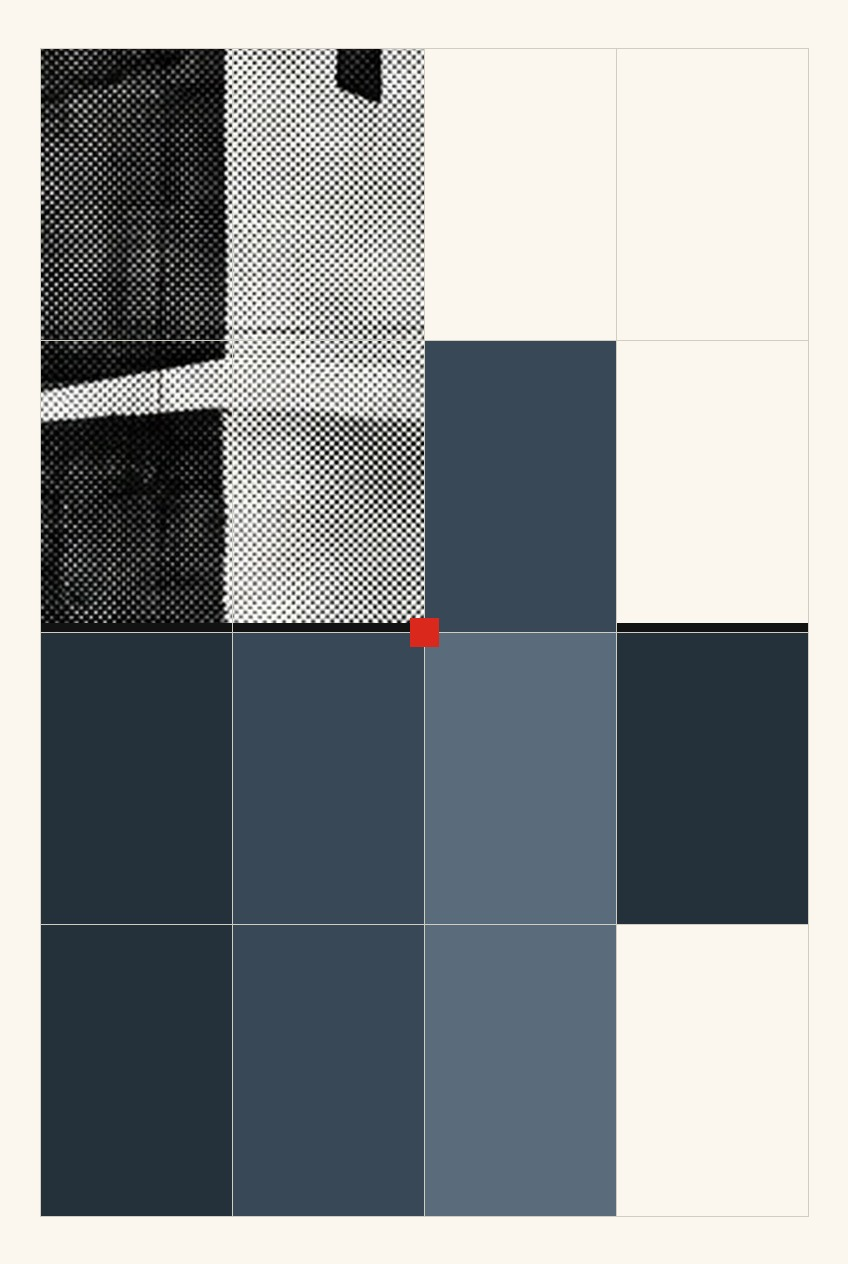
\includegraphics[width=\linewidth,height=0.92in,keepaspectratio]{plates/swiss/landmark-01.jpg}}%
    }{%
      \PackageError{pd-book-contents}{Missing chapter plate \pd@tocplatepath}%
        {Restore the chapter's edition-specific plate before building the Book.}%
    }%
  }}
% A fresh page for a part keeps its existing art and the first chapter together.
% The image is a visual locator for the same part plate encountered in the body.
\renewcommand*\l@part[2]{%
  \ifnum\pd@tocpart=0
    \par\addvspace{24pt}%
  \else
    \ifnum\pd@tocpart>\pdpartcount
      \Needspace*{14\baselineskip}\addvspace{24pt}%
    \else\clearpage\fi
  \fi
  \advance\pd@tocpart\@ne
  \pd@tocafterparttrue
  \ifnum\pd@tocpart>\pdpartcount
    \def\pd@toccolor{hhink}%
    {\pdtextface\LARGE\bfseries #1\hfill #2\par}%
    \vspace{9pt}\noindent\rule{\linewidth}{0.7pt}\par\vspace{12pt}%
  \else
    \edef\pd@toccolor{\csname pd@tocpartcolor@\the\pd@tocpart\endcsname}%
    \noindent
    \begin{minipage}[t]{0.29\linewidth}\vspace{0pt}%
      \expandafter\pd@tocplate\expandafter{\csname pd@tocpartart@\the\pd@tocpart\endcsname}%
    \end{minipage}\hfill
    \begin{minipage}[t]{0.66\linewidth}\vspace{0pt}\pdtextface\raggedright
      {\Large\bfseries\color{\pd@toccolor}#1\par}%
      \vspace{7pt}%
      {\small\csname pd@tocpartblurb@\the\pd@tocpart\endcsname\par}%
      \vspace{7pt}{\small Part opens on page #2\par}%
    \end{minipage}\par
    \vspace{13pt}\noindent{\color{\pd@toccolor}\rule{\linewidth}{1.1pt}}\par\vspace{10pt}%
  \fi\nobreak}
\newcommand*\l@chapter[2]{%
  \ifnum\pd@tocpart=0
    \Needspace*{15\baselineskip}\addvspace{22pt}%
    \noindent\begin{minipage}[t]{0.23\linewidth}\vspace{0pt}%
      \expandafter\pd@tocchapterplate\expandafter{\csname pd@tocchapterart@0\endcsname}%
    \end{minipage}\hfill
    \begin{minipage}[t]{0.72\linewidth}\vspace{0pt}%
    \begingroup
      \pdtextface\large\bfseries\color{\pd@toccolor}%
      \parindent\z@\rightskip 2.5em\parfillskip -2.5em
      \let\numberline\pd@tocchapternumber
      #1\nobreak\hfill\makebox[2.5em][r]{#2}\par
    \endgroup\nobreak
    \vspace{5pt}%
    {\rmfamily\small\raggedright
      \csname pd@tocchapterclaim@0\endcsname\par
      \edef\pd@tocnotename{pd@tocchapternote@0}%
      \expandafter\ifx\csname\pd@tocnotename\endcsname\@empty\else
        \vspace{3pt}{\itshape\csname\pd@tocnotename\endcsname\par}%
      \fi}%
    \end{minipage}\par\nobreak\vspace{10pt}%
  \else
    \ifpd@tocafterpart\pd@tocafterpartfalse\else
      \Needspace*{15\baselineskip}\addvspace{22pt}%
    \fi
    \advance\pd@tocchapter\@ne
    \noindent\begin{minipage}[t]{0.23\linewidth}\vspace{0pt}%
      \expandafter\pd@tocchapterplate\expandafter{\csname pd@tocchapterart@\the\pd@tocchapter\endcsname}%
    \end{minipage}\hfill
    \begin{minipage}[t]{0.72\linewidth}\vspace{0pt}%
    \begingroup
      \pdtextface\large\bfseries\color{\pd@toccolor}%
      \parindent\z@\rightskip 2.5em\parfillskip -2.5em
      \let\numberline\pd@tocchapternumber
      #1\nobreak\hfill\makebox[2.5em][r]{#2}\par
    \endgroup\nobreak
    \vspace{5pt}%
    {\rmfamily\small\raggedright
      \csname pd@tocchapterclaim@\the\pd@tocchapter\endcsname\par
      \edef\pd@tocnotename{pd@tocchapternote@\the\pd@tocchapter}%
      \expandafter\ifx\csname\pd@tocnotename\endcsname\@empty\else
        \vspace{3pt}{\itshape\csname\pd@tocnotename\endcsname\par}%
      \fi}%
    \end{minipage}\par\nobreak\vspace{10pt}%
  \fi}
\newcommand{\pd@tocchapternumber}[1]{#1\enspace}
% A quiet number gutter and one aligned page column. Subsections indent only
% their numbers; long titles keep a generous measure and wrap as hanging text.
\renewcommand*\l@section[2]{%
  \addvspace{5pt}\begingroup\pdtextface\normalsize\bfseries
    \@dottedtocline{1}{0pt}{3.8em}{#1}{#2}%
  \endgroup\nobreak}
\renewcommand*\l@subsection[2]{%
  \begingroup\pdtextface\small
    \@dottedtocline{2}{1.2em}{4.4em}{#1}{#2}%
  \endgroup}
\renewcommand*\l@subsubsection[2]{%
  \begingroup\color{hhgray}\pdcaptionface\footnotesize
    \@dottedtocline{3}{2.4em}{5em}{#1}{#2}%
  \endgroup}
\newcommand{\pdtableofcontents}{%
  \clearpage
  \newgeometry{inner=0.8in,outer=0.2in,top=0.85in,bottom=0.95in}%
  \begingroup
    \rmfamily\normalsize\color{hhink}%
    \parindent\z@\parskip\z@
    % Frontmatter roman folios need more room than the class's 1.55em gutter.
    \renewcommand\@pnumwidth{2.8em}\renewcommand\@tocrmarg{3.8em}%
    \setlength{\headwidth}{\textwidth}%
    \fancyhf{}\fancyhead[LE,RO]{\rmfamily\small Contents}%
    \fancyfoot[LE,RO]{\rmfamily\small\thepage}%
    \hypersetup{linkcolor=hhink}%
    \pd@tocpart=0 \pd@tocchapter=0 \pd@tocafterpartfalse
    \phantomsection\label{book:contents}%
    \pdfbookmark[0]{Contents}{book.contents}%
    {\pddisplayface\Huge\bfseries Contents\par}%
    \vspace{10pt}\noindent\rule{\linewidth}{1.1pt}\par\vspace{14pt}%
    {\pdtextface\large The complete argument, in \pdchaptercount{} chapters.\par}%
    \vspace{6pt}%
    \begin{minipage}{0.84\linewidth}\rmfamily\normalsize\raggedright
      Every chapter, section and subsection is listed here, followed by
      solutions, the result atlas, reference material and image credits.
      Titles and page numbers lead directly to their place in the book.
    \end{minipage}\par\vspace{20pt}%
    \@starttoc{toc}%
    \clearpage
  \endgroup
  \restoregeometry
}
\makeatother

% Hyperlink and cross-reference discipline (must stay last).
% Shared hyperlink and cross-reference discipline for the Book and its chapters.
% Load this LAST in every preamble: cleveref must follow hyperref and amsthm.
% hyperref itself is loaded earlier with [backref=page] (a load-time option).
% Twin copy under whitepaper/figures/ (byte-identical; checked by
% scripts/generate-mega-whitepaper.test.mjs).
%
% What a reader gets: live links on chapter titles, section numbers, theorems,
% figures, tables, equations, page numbers, and citations; PDF bookmarks three
% levels deep; and, at the end of every bibliography entry, the pages that cite it.
% Links are quiet: a warm dark ink one step lighter than body text, so the
% four part hues keep their meaning and an inline chapter title never competes
% with the part it sits in. Chrome pages (the front-matter map, part openers)
% recolor their own links locally.
\hypersetup{
  colorlinks=true,
  linkcolor=pdinkmuted,
  citecolor=pdinkmuted,
  urlcolor=pdinkmuted,
  filecolor=pdinkmuted,
  anchorcolor=pdink,
  bookmarksnumbered=true,
  bookmarksdepth=3,
  bookmarksopen=true,
  bookmarksopenlevel=1,
  breaklinks=true,
  linktoc=all,
  pdfauthor={Erich Owens},
  pdftitle={\pdchaptertitle},
  pdfsubject={\pdeditiontitle: \pdeditionsubtitle},
}

% Title-based chapter references. \pdchaplink{prefix}{text} is a live link to
% the chapter inside the Book (the Book's preamble defines it before loading this
% file); in a standalone chapter it is plain text. Prose uses \pdchapref, which
% sets the title in italics; the locator map uses \pdchaplink directly.
\providecommand{\pdchaplink}[2]{#2}
\DeclareRobustCommand{\pdchapref}[2]{\pdchaplink{#1}{\emph{#2}}}

% \ifpdbook -- true in the assembled Book, false otherwise.
%
% WHY THIS EXISTED. A drawing that two chapters both \input prints twice in the
% Book, under two figure numbers. The fix is for the chapter that develops the
% idea to keep the figure and the other to point at it -- but the standalone
% edition of a chapter had nowhere to point, and rewriting the prose outright
% removed five figures from harbor-economy-whitepaper.pdf and left it telling a
% conference reader that a ceremony is "drawn in The Federated Harbor", a
% document that reader did not have.
%
% WHERE IT STANDS NOW. The per-chapter PDFs are retired: the Book is the one
% document, so \ifpdbook is true in every build that renders, and the \else
% branches are source with no output. They are still here, and still read by
% check_duplicate_figures.py (which must not count an \else \input as a Book
% input) -- but nothing prints them, and nothing new should be put in one.
% Whether to delete them is an open question; see the retirement PR.
%
% The divergence was per-build. A CONDITIONAL and not a two-argument macro:
% the generator inlines each \input, so a figure branch is a whole table or
% tikzpicture, and as a macro argument that is scanned as one token list --
% which is how \pdinbook produced "runaway argument" on the first attempt.
% \ifpdbook skips the untaken branch at the TeX level instead.
%
% Declared unconditionally and defaulting FALSE, which is the standalone
% answer. The Book's preamble sets \pdbooktrue immediately after loading
% this file. A guard here would have to mention \ifpdbook or \newif inside a
% branch TeX may skip, and a conditional token in skipped text is counted as
% a nested \if -- which is how two attempts at a guard both produced
% "Incomplete \ifdefined". Ordering is cheaper than cleverness.
\newif\ifpdbook

% cleveref: "Theorem 3.1", "Figure 2.4", "Section 1.3", capitalised, never
% abbreviated, with the whole phrase clickable. Names are declared explicitly
% because the theorem environments are created before this file is loaded.
\usepackage[nameinlink,capitalise,noabbrev]{cleveref}
\crefname{pdchapter}{Chapter}{Chapters}
\crefname{part}{Part}{Parts}
\crefname{appendix}{Appendix}{Appendices}
\crefname{definition}{Definition}{Definitions}
\crefname{theorem}{Theorem}{Theorems}
\crefname{lemma}{Lemma}{Lemmas}
\crefname{proposition}{Proposition}{Propositions}
\crefname{corollary}{Corollary}{Corollaries}
\crefname{conjecture}{Conjecture}{Conjectures}
\crefname{property}{Property}{Properties}
\crefname{protocol}{Protocol}{Protocols}
\crefname{lsprotocol}{Protocol}{Protocols}
\crefname{stpprotocol}{Protocol}{Protocols}
\crefname{heprotocol}{Protocol}{Protocols}
\crefname{remark}{Remark}{Remarks}
\crefname{lstlisting}{Listing}{Listings}
\crefname{exercise}{Exercise}{Exercises}
\crefname{solution}{Solution}{Solutions}
\Crefname{pdchapter}{Chapter}{Chapters}
\Crefname{lstlisting}{Listing}{Listings}
\Crefname{exercise}{Exercise}{Exercises}
\Crefname{solution}{Solution}{Solutions}

% Back-references: "^ Cited on pages 12, 40, and 87." after every bibliography
% entry, each page number a live link back to the page that cited the work.
% Distinct pages only (#3/#4).
%
% The page numbers used to be wrapped in \color{hhgray} along with the words,
% which painted over the link colour hyperref had just given them: the links
% were there -- 29 annotations on a typical bibliography page -- and looked
% exactly like the grey prose around them, so nobody knew they could click.
% Restoring the quiet link colour would not have fixed it either; pdinkmuted
% against hhgray is 1.53:1, which is no signal at footnote size.
%
% So the numbers take pdcobalt (7.55:1 on the cream, and a hue a reader cannot
% mistake for grey), and the line opens with the return arrow this book already
% uses to send a solution back to its exercise. This is a deliberate exception
% to the quiet-link discipline above, and the reason is that back-matter
% navigation is the one place where the link IS the content: in prose the
% surrounding sentence tells you a phrase is a destination, and in a
% bibliography nothing does.
\renewcommand*{\backref}[1]{}
\renewcommand*{\backrefalt}[4]{%
  \ifcase #3\relax
  \or {\footnotesize{\color{hhgray}$\uparrow$~Cited on page}~{\hypersetup{linkcolor=pdcobalt}#4}{\color{hhgray}.}}%
  \else {\footnotesize{\color{hhgray}$\uparrow$~Cited on pages}~{\hypersetup{linkcolor=pdcobalt}#4}{\color{hhgray}.}}%
  \fi}
\renewcommand*{\backrefsep}{, }
\renewcommand*{\backreftwosep}{ and }
\renewcommand*{\backreflastsep}{, and }

% \ifpdbook is declared (false) in pd-hyperlinks; the Book turns it on here,
% AFTER the load, so nothing has to guard the \newif. It selects the Book
% branch wherever a chapter and its standalone paper must diverge -- a
% figure the Book prints once and cross-references, which the paper carries
% its own copy of.
\pdbooktrue

% ---------------------------------------------------------------------------
% Captioned exhibits must fit the text column: the outside margin is reserved
% for their captions. Record true ink width and warn on overflow; the matching
% PDF audit rejects it. Never hide an oversized figure by shrinking its type
% or moving its caption below it. The legacy spill/scale path below applies
% only to non-floating inline artwork and remains separately reviewable.
% ---------------------------------------------------------------------------
\usepackage{changepage}
\strictpagecheck
\newlength{\pdfullwidth}\setlength{\pdfullwidth}{\dimexpr\textwidth+\marginparsep+\marginparwidth\relax}
\makeatletter
% pgf hands every finished picture (tikzpicture, pgfplots axis, inline \tikz)
% to \pgfsys@typesetpicturebox with its width known; the hook decides where it
% goes. Nested pictures pass through untouched (their box is narrower than the
% line they sit in).
\newsavebox{\pd@picbox}
\let\pd@typesetpicturebox\pgfsys@typesetpicturebox
\def\pgfsys@typesetpicturebox#1{%
  \sbox{\pd@picbox}{\pd@typesetpicturebox#1}%
  % Figure-band recording for \pd@placemargin's centering (pd-pedagogy.tex):
  % from THIS box's own \ht/\dp, not from \pagetotal at \end{figure}. The
  % latter was tried first and does not work -- for an [H] float the
  % package defers inserting the box into the main vertical list past
  % \end{figure} itself, so \pagetotal read there (even settled) still
  % under-reads by the whole figure and \pd@figbot came out equal to
  % \pd@figtop on every figure measured. \pagetotal HERE, mid-paragraph
  % while pgf is still handing us the finished picture box, is the page
  % height immediately above where this box is about to be placed, and the
  % box's own \ht+\dp is its true rendered height regardless of how (or
  % whether) it gets rescaled below -- both read before any resizing, which
  % is fine: \pd@placemargin only wants the figure's vertical band, and
  % \resizebox below does not change a box's VERTICAL position, only its
  % size, and \centering does not move a box vertically at all.
  \ifpdmargincolumn
    \xdef\pd@figpage{\number\value{page}}%
    \global\pd@figtop=\pagetotal
    \global\pd@figbot=\dimexpr\pagetotal+\ht\pd@picbox+\dp\pd@picbox\relax
  \fi
  % the box has no width of its own yet; pgf sets it from the bounding box
  \@tempdima=\dimexpr\pgf@picmaxx-\pgf@picminx\relax
  \ifpd@captionfloat
    \ifdim\@tempdima>\pd@exhibitinkwidth
      \global\pd@exhibitinkwidth=\@tempdima\fi
  \fi
  \ifdim\@tempdima>\dimexpr\linewidth+1pt\relax
    \ifpd@captionfloat
      % The outer margin belongs to the caption. Preserve the bad geometry
      % for the audit; never conceal it by shrinking type or dropping captions.
      \PackageWarning{pd-book}{PD-EXHIBIT-WIDE: \@captype\space
        \@nameuse{the\@captype}; width=\the\@tempdima; limit=\the\linewidth}%
      \makebox[\linewidth][c]{\usebox{\pd@picbox}}%
    \else
    \ifdim\linewidth<\dimexpr\textwidth-1pt\relax
      \ifpdmarginevidence
        \PackageError{pd-book}{Margin evidence exceeds its native width}%
          {Redraw to marginparwidth; shrinking labels is not permitted.}%
        \usebox{\pd@picbox}%
      \else
      % inside a minipage, a margin note or a table cell: fit the box we are in
      \PackageWarning{pd-book}{picture \the\wd\pd@picbox\space wide scaled to a \the\linewidth\space box}%
      \resizebox{\linewidth}{!}{\usebox{\pd@picbox}}%
      \fi
    \else
      \ifdim\wd\pd@picbox>\pdfullwidth
        \PackageWarning{pd-book}{picture \the\wd\pd@picbox\space wide scaled to the full width}%
        \sbox{\pd@picbox}{\resizebox{\pdfullwidth}{!}{\usebox{\pd@picbox}}}%
      \else
        \PackageInfo{pd-book}{picture \the\wd\pd@picbox\space wide set full width}%
      \fi
      % Strict page checking records the box's shipped page in the aux file,
      % so a floated picture uses its physical leaf rather than the page TeX
      % happened to be composing when the hook fired. Odd rectos spill right;
      % even versos spill left. The text measure never shrinks to make room.
      \checkoddpage
      \ifoddpage
        \makebox[\textwidth][l]{\usebox{\pd@picbox}}%
      \else
        \makebox[\textwidth][r]{\usebox{\pd@picbox}}%
      \fi
    \fi
    \fi
  \else
    \usebox{\pd@picbox}%
  \fi}
\NewDocumentCommand\pdpagecentered{O{\pdfullwidth} m}{%
  \par\noindent\checkoddpage
  \makebox[\textwidth][c]{%
    \ifoddpage\hspace*{0.45in}\else\hspace*{-0.45in}\fi
    \makebox[#1][c]{#2}%
  }\par
}
\NewDocumentCommand\pdpagecaption{O{} m O{}}{%
  \par\vspace{6pt}%
  \begingroup
  \let\pd@captiontype\relax
  \pd@routecaptionfalse
  \noindent\checkoddpage
  \makebox[\textwidth][c]{%
    \ifoddpage\hspace*{0.45in}\else\hspace*{-0.45in}\fi
    \begin{minipage}{\dimexpr\pdfullwidth-0.2in\relax}%
      \if\relax\detokenize{#1}\relax\caption{#2}\else\caption[#1]{#2}\fi
      \if\relax\detokenize{#3}\relax\else\label{#3}\fi
    \end{minipage}%
  }%
  \endgroup
  \par
}
\NewDocumentCommand\pdwidecaption{O{} m O{}}{%
  \pdpagecaption[#1]{#2}[#3]%
}
\makeatother

\makeatletter
\let\pgfsys@typesetpicturebox\pd@typesetpicturebox
\makeatother
\geometry{a4paper,landscape,top=0.6cm,bottom=0.6cm,left=1.0cm,right=1.0cm}

\pagestyle{fancy}
\fancyhf{}
\renewcommand{\headrulewidth}{0.4pt}
\renewcommand{\footrulewidth}{0.3pt}
\fancyhead[L]{\pdgrotesk\footnotesize\bfseries PORT DADDY WHITE PAPER \ \textperiodcentered \ \ \textsc{Architectural Figure Reconciliation Audit}}
\fancyhead[R]{\pdgrotesk\footnotesize\bfseries Visual Proof \& Comparative Verification \ \textperiodcentered \ \ Page \thepage\ of 18}
\fancyfoot[L]{\pdgrotesk\scriptsize\textbf{Status:} 100\% Reconciled \ \textperiodcentered \ \ Native Vector TikZ/PGF \ \textperiodcentered \ \ Local XeLaTeX Compilation \ \textperiodcentered \ \ \$0.00 Spend}
\fancyfoot[R]{\pdgrotesk\scriptsize Governing AI Agents: The Harbor, the Person, and the Economy}

\newsavebox{\pdfigbox}
\newsavebox{\pdscaledbox}
\newdimen\pdmaxh
\newdimen\pdmaxw
\newdimen\pdcurh
\newdimen\pdcurw
\newcommand{\pdautoscale}[2]{% #1 max height, #2 max width
  \pdmaxh=#1\relax
  \pdmaxw=#2\relax
  \sbox{\pdscaledbox}{\usebox{\pdfigbox}}%
  \pdcurh=\dimexpr\ht\pdscaledbox+\dp\pdscaledbox\relax
  \pdcurw=\wd\pdscaledbox
  \ifdim\dimexpr\pdcurw * 100 / \pdmaxw\relax > \dimexpr\pdcurh * 100 / \pdmaxh\relax
    \resizebox{\pdmaxw}{!}{\usebox{\pdscaledbox}}%
  \else
    \resizebox{!}{\pdmaxh}{\usebox{\pdscaledbox}}%
  \fi
}

\begin{document}

% =========================================================================
% PAGE 1: Figure 0.1
% =========================================================================
\noindent
\begin{minipage}[t]{\linewidth}
  \noindent{\pdgrotesk\large\bfseries Figure 0.1 \textperiodcentered\ Proposition 1 Mechanics: Serial Write Arbitration}\hfill
  {\pdgrotesk\footnotesize\color{hhgray} Section 0.2.1 · Theoretical Foundations of Agency · Single-Writer Mutex}\\
  \vspace*{0.03cm}
  \noindent{\color{hhgray!40}\rule{\linewidth}{0.5pt}}
\end{minipage}

\vspace*{0.05cm}
\noindent
\begin{minipage}[t]{0.492\linewidth}
  \begin{tcolorbox}[
    colback=pdslate!4,colframe=pdslate!70!black,arc=1.5pt,
    boxrule=0.6pt,top=1.5pt,bottom=1.5pt,left=4pt,right=4pt,
    title={\pdgrotesk\footnotesize\bfseries \color{white} A. AI-Generated Raster Prototype (Diffusion / Nano Banana) \hfill \texttt{.jpg / .png}}
  ]
    \begin{minipage}[c][8.3cm][c]{\linewidth}
      \centering
      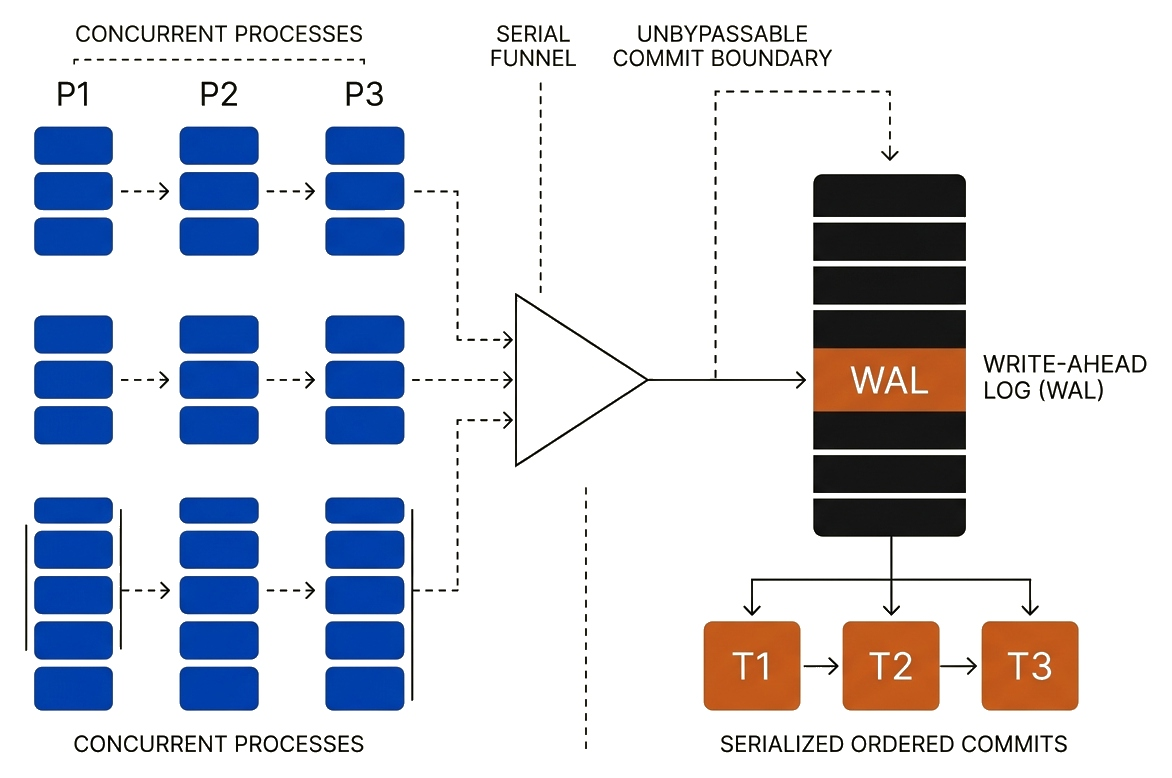
\includegraphics[width=\linewidth,height=8.0cm,keepaspectratio]{figures/fig-spark-prop1-funnel.jpg}
    \end{minipage}
    \tcblower
    \begin{minipage}[t][2.0cm][t]{\linewidth}
      \pdgrotesk\scriptsize
      \textbf{\color{pderror!90!black} Artifact \& Limitation Audit:}\\
      \begin{itemize}[leftmargin=9pt,itemsep=0pt,topsep=0.5pt,parsep=0pt]
        \item Lossy raster rendering; blurry text on commit blocks and process queues
        \item Inexact funnels; non-orthogonal connections between writer processes and queue
        \item Opaque binary blob (78 KB); cannot review or diff structural updates in git
      \end{itemize}
    \end{minipage}
  \end{tcolorbox}
\end{minipage}\hfill
\begin{minipage}[t]{0.492\linewidth}
  \begin{tcolorbox}[
    colback=pdcobalt!3,colframe=pdcobalt!85!black,arc=1.5pt,
    boxrule=0.7pt,top=1.5pt,bottom=1.5pt,left=4pt,right=4pt,
    title={\pdgrotesk\footnotesize\bfseries \color{white} B. Authoritative Native Vector Replacement \hfill \texttt{.tex / TikZ / PGF}}
  ]
    \begin{minipage}[c][8.3cm][c]{\linewidth}
      \centering
      \sbox{\pdfigbox}{% fig-spark-prop1-funnel.tex
% Proposition 1: Serial Write Arbitration (The Single-Writer Kernel)
% Faithful 100% native vector Swiss TikZ reconstruction of fig-spark-prop1-funnel.jpg.
% Full-width (15.0cm = \pdfullwidth), pure white ground, Swiss typography.
% Strict adherence to Harbor Figure Standard (v2):
% - Sentence case for all titles and labels (never ALL-CAPS).
% - High Tufte data-ink ratio (quiet neutral tones, minimal non-data ink, crisp borders).
% - Typographic law: \pdfiglabelsize (\footnotesize), pd title, pd label; zero inline \fontsize.
% - Line weight ladder: 0.5pt (hairline/guides), 0.9pt (rules/arrows/borders), 1.6pt (spine).
% - Semantic palette: pdcobalt (concurrent processes), pdrust (WAL commit climax), pdslate (neutral frames).
\pdfigurehue{pdcobalt}%
\begin{tikzpicture}[pd figure,x=1cm,y=1cm]
  \tikzset{
    pblock/.style={
      draw=pdcobalt,
      line width=0.7pt,
      fill=pdcobalt!20,
      rounded corners=2pt
    },
    walframe/.style={
      draw=pdslate!80!black,
      line width=0.5pt,
      fill=pdslate!10,
      rounded corners=1.5pt
    },
    walactive/.style={
      draw=pdrust!90!black,
      line width=0.9pt,
      fill=pdrust,
      rounded corners=2pt
    },
    commitbox/.style={
      draw=pdrust!90!black,
      line width=0.9pt,
      fill=pdrust,
      rounded corners=2.5pt
    },
    funnelarrow/.style={
      ->,
      >=Stealth,
      line width=0.9pt,
      draw=pdink
    },
    dashedconnect/.style={
      ->,
      >=Stealth,
      line width=0.7pt,
      dashed,
      draw=pdink!80!black
    }
  }

  % =========================================================================
  % LEFT REGION: CONCURRENT PROCESSES (x in [0.6, 5.0])
  % =========================================================================
  % Top Header & Bracket (Sentence case)
  \node[pd title,anchor=center,text=pdink] at (2.8, 9.4) {%
    Concurrent processes%
  };
  \draw[line width=0.5pt,dashed,draw=pdink!60!black]
    (0.9, 8.95) -- (0.9, 9.10) -- (4.7, 9.10) -- (4.7, 8.95);

  % Column Headers: P1, P2, P3
  \node[pd title,anchor=center,text=pdink] at (1.4, 8.5) {P1};
  \node[pd title,anchor=center,text=pdink] at (2.8, 8.5) {P2};
  \node[pd title,anchor=center,text=pdink] at (4.2, 8.5) {P3};

  % --- Row 1 (Top Stack: 3 blocks per column) ---
  \foreach \col/\cx in {1/1.4, 2/2.8, 3/4.2} {
    \filldraw[pblock] (\cx-0.5, 7.60) rectangle (\cx+0.5, 8.05);
    \filldraw[pblock] (\cx-0.5, 7.05) rectangle (\cx+0.5, 7.50);
    \filldraw[pblock] (\cx-0.5, 6.50) rectangle (\cx+0.5, 6.95);
  }
  \draw[dashedconnect] (1.95, 7.27) -- (2.25, 7.27);
  \draw[dashedconnect] (3.35, 7.27) -- (3.65, 7.27);

  % --- Row 2 (Middle Stack: 3 blocks per column) ---
  \foreach \col/\cx in {1/1.4, 2/2.8, 3/4.2} {
    \filldraw[pblock] (\cx-0.5, 5.45) rectangle (\cx+0.5, 5.90);
    \filldraw[pblock] (\cx-0.5, 4.90) rectangle (\cx+0.5, 5.35);
    \filldraw[pblock] (\cx-0.5, 4.35) rectangle (\cx+0.5, 4.80);
  }
  \draw[dashedconnect] (1.95, 5.12) -- (2.25, 5.12);
  \draw[dashedconnect] (3.35, 5.12) -- (3.65, 5.12);

  % --- Row 3 (Bottom Stack: 5 blocks per column) ---
  \foreach \col/\cx in {1/1.4, 2/2.8, 3/4.2} {
    \filldraw[pblock] (\cx-0.5, 3.35) rectangle (\cx+0.5, 3.75);
    \filldraw[pblock] (\cx-0.5, 2.85) rectangle (\cx+0.5, 3.25);
    \filldraw[pblock] (\cx-0.5, 2.35) rectangle (\cx+0.5, 2.75);
    \filldraw[pblock] (\cx-0.5, 1.85) rectangle (\cx+0.5, 2.25);
    \filldraw[pblock] (\cx-0.5, 1.35) rectangle (\cx+0.5, 1.75);
  }
  % Vertical guide lines on row 3 (P1 and P3)
  \draw[line width=0.5pt,draw=pdink!50!black] (0.8, 1.35) -- (0.8, 3.75);
  \draw[line width=0.5pt,draw=pdink!50!black] (4.8, 1.35) -- (4.8, 3.75);
  \draw[dashedconnect] (1.95, 2.55) -- (2.25, 2.55);
  \draw[dashedconnect] (3.35, 2.55) -- (3.65, 2.55);

  % Bottom Label for Processes (Sentence case)
  \node[pd label,anchor=center,text=pdink] at (2.8, 0.7) {%
    Concurrent processes%
  };

  % =========================================================================
  % CONVERGENCE DASHED LINES INTO FUNNEL
  % =========================================================================
  % From Row 1 (y=7.27) -> down to y=5.6 -> funnel
  \draw[dashedconnect] (4.7, 7.27) -- (5.4, 7.27) -- (5.4, 5.6) -- (6.1, 5.6);
  % From Row 2 (y=5.12) -> funnel
  \draw[dashedconnect] (4.7, 5.12) -- (6.1, 5.12);
  % From Row 3 (y=2.55) -> up to y=4.6 -> funnel
  \draw[dashedconnect] (4.7, 2.55) -- (5.4, 2.55) -- (5.4, 4.6) -- (6.1, 4.6);

  % =========================================================================
  % CENTER REGION: SERIAL FUNNEL & COMMIT BOUNDARY (x in [6.1, 8.5])
  % =========================================================================
  % Funnel Polygon (Triangle pointing right)
  \filldraw[draw=pdink,line width=0.9pt,fill=pdpage]
    (6.1, 3.6) -- (7.8, 5.1) -- (6.1, 6.6) -- cycle;

  % Serial Funnel Annotation (Sentence case)
  \node[pd title,anchor=center,align=center,text=pdink] at (6.3, 9.4) {%
    Serial\\funnel%
  };
  \draw[line width=0.5pt,dashed,draw=pdink!60!black] (6.3, 8.8) -- (6.3, 6.4);

  % Central vertical dashed divider line
  \draw[line width=0.5pt,dashed,draw=pdink!60!black] (7.0, 3.2) -- (7.0, 0.4);

  % Commit boundary arrow from funnel tip to WAL
  \draw[funnelarrow,line width=0.9pt] (7.8, 5.1) -- (9.9, 5.1);

  % Unbypassable Commit Boundary Annotation (Sentence case, centered over horizontal path 8.7 -> 11.0)
  \node[pd title,anchor=center,align=center,text=pdink] at (9.9, 9.4) {%
    Unbypassable\\commit boundary%
  };
  \draw[dashedconnect] (8.7, 5.1) -- (8.7, 8.8) -- (11.0, 8.8) -- (11.0, 8.05);

  % =========================================================================
  % RIGHT REGION: WRITE-AHEAD LOG (WAL) & ORDERED COMMITS (x in [10.0, 14.8])
  % =========================================================================
  % WAL Stack Box (centered at x = 11.0)
  % 4 neutral frames above (quiet slate tint, 0.5pt border, high Tufte data-ink ratio)
  \filldraw[walframe] (10.0, 7.55) rectangle (12.0, 8.00);
  \filldraw[walframe] (10.0, 7.00) rectangle (12.0, 7.45);
  \filldraw[walframe] (10.0, 6.45) rectangle (12.0, 6.90);
  \filldraw[walframe] (10.0, 5.90) rectangle (12.0, 6.35);

  % Highlighted Active WAL Frame (Warm Rust Climax State)
  \filldraw[walactive] (10.0, 5.00) rectangle (12.0, 5.80);
  \node[pd title,anchor=center,text=white] at (11.0, 5.40) {%
    WAL%
  };

  % 3 neutral frames below
  \filldraw[walframe] (10.0, 4.35) rectangle (12.0, 4.80);
  \filldraw[walframe] (10.0, 3.80) rectangle (12.0, 4.25);
  \filldraw[walframe] (10.0, 3.25) rectangle (12.0, 3.70);

  % Label next to WAL Stack (Sentence case)
  \node[pd title,anchor=west,align=left,text=pdink] at (12.2, 5.40) {%
    Write-ahead\\log (WAL)%
  };

  % --- Serialized Ordered Commits ---
  % Fork arrows down from WAL base (y = 3.25)
  \draw[line width=0.9pt,draw=pdink] (11.0, 3.25) -- (11.0, 2.7);
  \draw[funnelarrow,line width=0.9pt] (11.0, 2.7) -- (9.2, 2.7) -- (9.2, 2.2);
  \draw[funnelarrow,line width=0.9pt] (11.0, 2.7) -- (11.0, 2.2);
  \draw[funnelarrow,line width=0.9pt] (11.0, 2.7) -- (12.8, 2.7) -- (12.8, 2.2);

  % Commit Boxes: T1 -> T2 -> T3
  \filldraw[commitbox] (8.6, 1.25) rectangle (9.8, 2.2);
  \node[pd title,anchor=center,text=white] at (9.2, 1.72) {T1};

  \draw[funnelarrow,line width=0.9pt] (9.9, 1.72) -- (10.3, 1.72);

  \filldraw[commitbox] (10.4, 1.25) rectangle (11.6, 2.2);
  \node[pd title,anchor=center,text=white] at (11.0, 1.72) {T2};

  \draw[funnelarrow,line width=0.9pt] (11.7, 1.72) -- (12.1, 1.72);

  \filldraw[commitbox] (12.2, 1.25) rectangle (13.4, 2.2);
  \node[pd title,anchor=center,text=white] at (12.8, 1.72) {T3};

  % Bottom Label for Ordered Commits (Sentence case)
  \node[pd label,anchor=center,text=pdink] at (11.0, 0.7) {%
    Serialized ordered commits%
  };

\end{tikzpicture}
}
      \pdautoscale{8.0cm}{\linewidth}
    \end{minipage}
    \tcblower
    \begin{minipage}[t][2.0cm][t]{\linewidth}
      \pdgrotesk\scriptsize
      \textbf{{\color{pdcobalt} Engineering \& Typography Guarantees:}}\\
      \begin{itemize}[leftmargin=9pt,itemsep=0pt,topsep=0.5pt,parsep=0pt]
        \item Native vector precision with mathematical bezier funnel curve
        \item Strict 3-tier hierarchy: Concurrent processes (pdcobalt), Funnel, Commit boundary
        \item Active WAL highlighted in pdrust; 100\% diffable LaTeX source code
      \end{itemize}
    \end{minipage}
  \end{tcolorbox}
\end{minipage}

\vspace*{0.05cm}
\noindent
\begin{tcolorbox}[
  colback=hhpaper,colframe=hhgray!35,arc=1.5pt,boxrule=0.4pt,
  top=1.5pt,bottom=1.5pt,left=6pt,right=6pt
]
  \pdgrotesk\scriptsize
  \noindent
  \textbf{Visual Substrate:} Lossy Bitmap Raster $\rightarrow$ \textbf{\color{pdcobalt}Native PDF / PostScript Vector}\hfill
  \textbf{Text Engine:} Pixelated Approximations $\rightarrow$ \textbf{\color{pdcobalt}Book Typography (OpenType)}\hfill
  \textbf{Resolution:} Fixed DPI Limit $\rightarrow$ \textbf{\color{pdcobalt}Infinite Resolution ($\infty$)}\hfill
  \textbf{Status:} \textbf{\color{pdteal}RECONCILED \& VERIFIED}
\end{tcolorbox}
\clearpage

% =========================================================================
% PAGE 2: Figure 0.2
% =========================================================================
\noindent
\begin{minipage}[t]{\linewidth}
  \noindent{\pdgrotesk\large\bfseries Figure 0.2 \textperiodcentered\ Proposition 2 Mechanics: Monotonic Capability Attenuation}\hfill
  {\pdgrotesk\footnotesize\color{hhgray} Section 0.2.2 · Security Architecture · The Anchor Protocol \& Macaroons}\\
  \vspace*{0.03cm}
  \noindent{\color{hhgray!40}\rule{\linewidth}{0.5pt}}
\end{minipage}

\vspace*{0.05cm}
\noindent
\begin{minipage}[t]{0.492\linewidth}
  \begin{tcolorbox}[
    colback=pdslate!4,colframe=pdslate!70!black,arc=1.5pt,
    boxrule=0.6pt,top=1.5pt,bottom=1.5pt,left=4pt,right=4pt,
    title={\pdgrotesk\footnotesize\bfseries \color{white} A. AI-Generated Raster Prototype (Diffusion / Nano Banana) \hfill \texttt{.jpg / .png}}
  ]
    \begin{minipage}[c][8.3cm][c]{\linewidth}
      \centering
      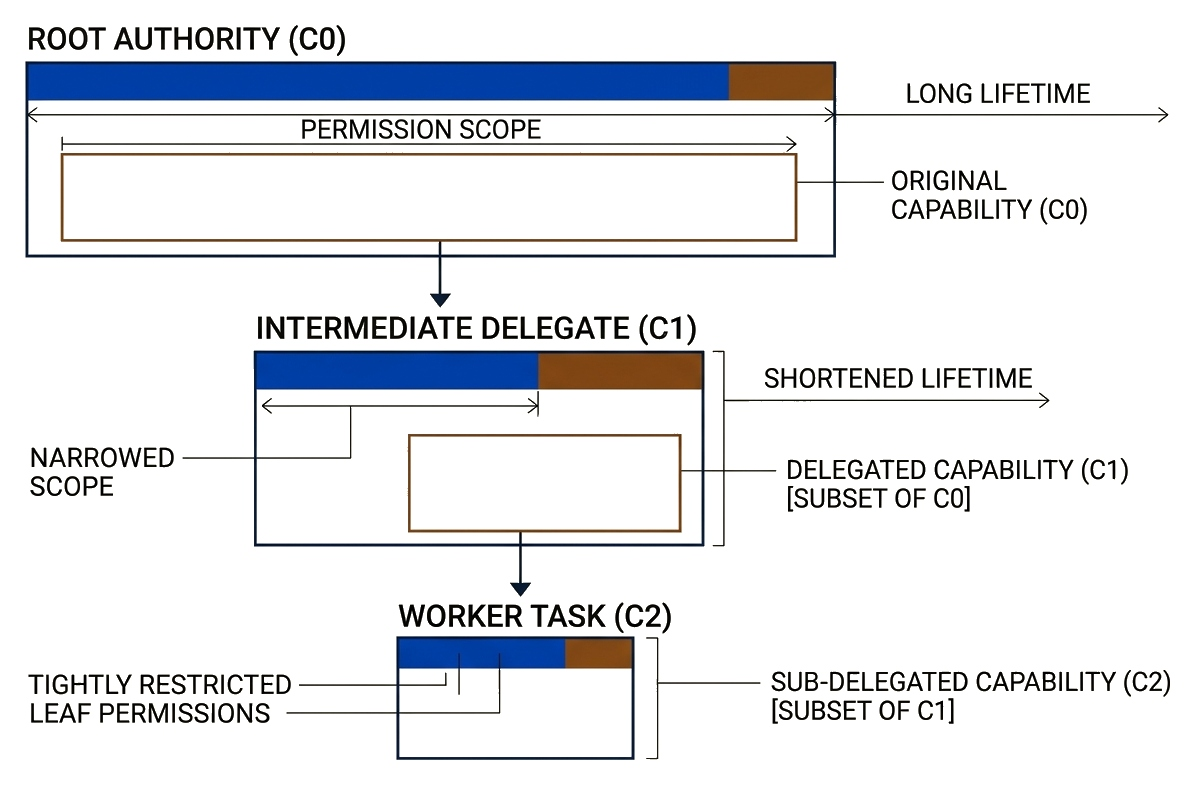
\includegraphics[width=\linewidth,height=8.0cm,keepaspectratio]{figures/fig-spark-prop2-attenuation.jpg}
    \end{minipage}
    \tcblower
    \begin{minipage}[t][2.0cm][t]{\linewidth}
      \pdgrotesk\scriptsize
      \textbf{\color{pderror!90!black} Artifact \& Limitation Audit:}\\
      \begin{itemize}[leftmargin=9pt,itemsep=0pt,topsep=0.5pt,parsep=0pt]
        \item Fuzzy badge typography and illegible caveat signatures
        \item Inconsistent arrow spacing and arbitrary delegation hops
        \item No formal attenuation constraint check visible in source asset
      \end{itemize}
    \end{minipage}
  \end{tcolorbox}
\end{minipage}\hfill
\begin{minipage}[t]{0.492\linewidth}
  \begin{tcolorbox}[
    colback=pdcobalt!3,colframe=pdcobalt!85!black,arc=1.5pt,
    boxrule=0.7pt,top=1.5pt,bottom=1.5pt,left=4pt,right=4pt,
    title={\pdgrotesk\footnotesize\bfseries \color{white} B. Authoritative Native Vector Replacement \hfill \texttt{.tex / TikZ / PGF}}
  ]
    \begin{minipage}[c][8.3cm][c]{\linewidth}
      \centering
      \sbox{\pdfigbox}{% fig-spark-prop2-attenuation.tex
% Proposition 2: Monotonic Capability Attenuation (The Anchor Protocol)
% Faithful 100% native vector Swiss TikZ reconstruction of fig-spark-prop2-attenuation.jpg.
% Full-width (15.0cm = \pdfullwidth), pure white ground, Swiss typography.
% Strict adherence to Harbor Figure Standard (v2):
% - Sentence case for all titles and labels (never ALL-CAPS).
% - High Tufte data-ink ratio (quiet neutral tones, minimal non-data ink, crisp borders).
% - Typographic law: \pdfiglabelsize (\footnotesize), pd title, pd label; zero inline \fontsize.
% - Line weight ladder: 0.5pt (hairline/guides), 0.9pt (rules/arrows/borders), 1.6pt (spine).
% - Semantic palette: pdcobalt (permission scope), pdrust (lifetime attenuation), pdink (text/rules).
\pdfigurehue{pdcobalt}%
\begin{tikzpicture}[pd figure,x=1cm,y=1cm]
  \tikzset{
    outerenvelope/.style={
      draw=pdink,
      line width=0.9pt,
      fill=pdpage,
      rounded corners=1.5pt
    },
    innerbox/.style={
      draw=pdink!80!black,
      line width=0.7pt,
      fill=pdpage,
      rounded corners=1.5pt
    },
    scopebar/.style={
      draw=pdcobalt,
      line width=0.7pt,
      fill=pdcobalt!20
    },
    timebar/.style={
      draw=pdrust,
      line width=0.7pt,
      fill=pdrust!20
    },
    dimline/.style={
      <->,
      >=Stealth,
      line width=0.5pt,
      draw=pdink!80!black
    },
    guideline/.style={
      line width=0.5pt,
      draw=pdink!60!black
    },
    descentarrow/.style={
      ->,
      >=Stealth,
      line width=0.9pt,
      draw=pdink
    }
  }

  % =========================================================================
  % TIER 1: ROOT AUTHORITY (C0) (y in [6.8, 9.8])
  % =========================================================================
  % Title (Sentence case)
  \node[pd title,anchor=south west,text=pdink] at (0.8, 9.55) {%
    Root authority ($C_0$)%
  };

  % Outer Envelope Box
  \draw[outerenvelope] (0.8, 7.0) rectangle (10.4, 9.5);

  % Top Horizontal Bar: Permission Scope (Blue) + Lifetime (Rust)
  \filldraw[scopebar] (0.8, 9.0) rectangle (9.1, 9.5);
  \filldraw[timebar] (9.1, 9.0) rectangle (10.4, 9.5);

  % Permission Scope Dimension Line (knockout text on line)
  \draw[dimline] (1.2, 8.75) -- (9.9, 8.75);
  \node[pd label,fill=pdpage,inner xsep=4pt,text=pdink] at (5.55, 8.75) {%
    Permission scope%
  };

  % Inner Capability Box (Original Capability C0)
  \draw[innerbox] (1.2, 7.2) rectangle (9.9, 8.4);

  % Label to the right of Inner Box
  \draw[guideline] (9.9, 7.8) -- (11.0, 7.8);
  \node[pd label,anchor=west,text=pdink] at (11.0, 7.8) {%
    Original capability ($C_0$)%
  };

  % Long Lifetime Dimension Arrow
  \draw[guideline] (10.4, 9.25) -- (10.4, 8.75);
  \draw[descentarrow] (10.4, 8.75) -- (14.6, 8.75)
    node[midway,above=2pt,pd label,text=pdink] {Long lifetime};

  % =========================================================================
  % DESCENT ARROW: TIER 1 -> TIER 2
  % =========================================================================
  \draw[descentarrow] (6.0, 7.0) -- (6.0, 6.85);

  % =========================================================================
  % TIER 2: INTERMEDIATE DELEGATE (C1) (y in [3.5, 6.2])
  % =========================================================================
  % Title (Sentence case)
  \node[pd title,anchor=south,text=pdink] at (6.0, 6.25) {%
    Intermediate delegate ($C_1$)%
  };

  % Outer Envelope Box
  \draw[outerenvelope] (3.4, 3.7) rectangle (8.7, 6.2);

  % Top Horizontal Bar: Narrowed Scope (Blue) + Shortened Lifetime (Rust)
  \filldraw[scopebar] (3.4, 5.7) rectangle (6.8, 6.2);
  \filldraw[timebar] (6.8, 5.7) rectangle (8.7, 6.2);

  % Narrowed Scope Dimension Line and Callout
  \draw[dimline] (3.4, 5.45) -- (6.8, 5.45);
  \draw[guideline] (5.1, 5.45) -- (5.1, 5.0) -- (2.6, 5.0);
  \node[pd label,anchor=east,align=right,text=pdink] at (2.5, 5.0) {%
    Narrowed\\scope%
  };

  % Inner Capability Box (Delegated Capability C1)
  \draw[innerbox] (5.2, 3.9) rectangle (8.4, 4.9);

  % Label to the right of Inner Box
  \draw[guideline] (8.4, 4.4) -- (9.6, 4.4);
  \node[pd label,anchor=west,align=left,text=pdink] at (9.6, 4.4) {%
    Delegated capability ($C_1$)\\[1pt]%
    \mdseries[subset of $C_0$]%
  };

  % Shortened Lifetime Bracket and Arrow
  \draw[guideline] (8.9, 6.2) -- (9.05, 6.2) -- (9.05, 3.7) -- (8.9, 3.7);
  \draw[descentarrow] (9.05, 5.45) -- (13.2, 5.45)
    node[midway,above=2pt,pd label,text=pdink] {Shortened lifetime};

  % =========================================================================
  % DESCENT ARROW: TIER 2 -> TIER 3
  % =========================================================================
  \draw[descentarrow] (6.5, 3.7) -- (6.5, 3.55);

  % =========================================================================
  % TIER 3: WORKER TASK (C2) (y in [0.8, 2.9])
  % =========================================================================
  % Title (Sentence case)
  \node[pd title,anchor=south,text=pdink] at (6.5, 2.95) {%
    Worker task ($C_2$)%
  };

  % Outer Envelope Box
  \draw[outerenvelope] (5.1, 1.0) rectangle (7.9, 2.9);

  % Top Horizontal Bar: Tightly Restricted Leaf Scope + Minimal Lifetime
  \filldraw[scopebar] (5.1, 2.5) rectangle (7.1, 2.9);
  \filldraw[timebar] (7.1, 2.5) rectangle (7.9, 2.9);

  % Vertical Subdivision Lines for Individual Leaf Permissions
  \draw[guideline] (5.8, 2.5) -- (5.8, 2.9);
  \draw[guideline] (6.4, 2.5) -- (6.4, 2.9);

  % Callouts for Tightly Restricted Leaf Permissions
  \draw[guideline] (5.7, 2.5) -- (5.7, 1.9) -- (3.9, 1.9);
  \draw[guideline] (6.3, 2.5) -- (6.3, 1.5) -- (3.9, 1.5);
  \node[pd label,anchor=east,align=right,text=pdink] at (3.8, 1.7) {%
    Tightly restricted\\leaf permissions%
  };

  % Right Bracket and Sub-delegated Capability Label
  \draw[guideline] (8.1, 2.9) -- (8.25, 2.9) -- (8.25, 1.0) -- (8.1, 1.0);
  \draw[guideline] (8.25, 1.95) -- (9.6, 1.95);
  \node[pd label,anchor=west,align=left,text=pdink] at (9.6, 1.95) {%
    Sub-delegated capability ($C_2$)\\[1pt]%
    \mdseries[subset of $C_1$]%
  };

\end{tikzpicture}
}
      \pdautoscale{8.0cm}{\linewidth}
    \end{minipage}
    \tcblower
    \begin{minipage}[t][2.0cm][t]{\linewidth}
      \pdgrotesk\scriptsize
      \textbf{{\color{pdcobalt} Engineering \& Typography Guarantees:}}\\
      \begin{itemize}[leftmargin=9pt,itemsep=0pt,topsep=0.5pt,parsep=0pt]
        \item Exact chained HMAC signatures with monotonic capability narrowing ($C_0 \supset C_1 \supset C_2$)
        \item Visual boundary enforcement: Attenuated tokens strictly subset parental scopes
        \item Systematic color-coding for root issuer, intermediary delegation, and leaf execution
      \end{itemize}
    \end{minipage}
  \end{tcolorbox}
\end{minipage}

\vspace*{0.05cm}
\noindent
\begin{tcolorbox}[
  colback=hhpaper,colframe=hhgray!35,arc=1.5pt,boxrule=0.4pt,
  top=1.5pt,bottom=1.5pt,left=6pt,right=6pt
]
  \pdgrotesk\scriptsize
  \noindent
  \textbf{Visual Substrate:} Lossy Bitmap Raster $\rightarrow$ \textbf{\color{pdcobalt}Native PDF / PostScript Vector}\hfill
  \textbf{Text Engine:} Pixelated Approximations $\rightarrow$ \textbf{\color{pdcobalt}Book Typography (OpenType)}\hfill
  \textbf{Resolution:} Fixed DPI Limit $\rightarrow$ \textbf{\color{pdcobalt}Infinite Resolution ($\infty$)}\hfill
  \textbf{Status:} \textbf{\color{pdteal}RECONCILED \& VERIFIED}
\end{tcolorbox}
\clearpage

% =========================================================================
% PAGE 3: Figure 0.3
% =========================================================================
\noindent
\begin{minipage}[t]{\linewidth}
  \noindent{\pdgrotesk\large\bfseries Figure 0.3 \textperiodcentered\ Proposition 3 Mechanics: Sealed Room Confinement}\hfill
  {\pdgrotesk\footnotesize\color{hhgray} Section 0.2.3 · Execution Isolation · Sandboxing \& Spend Caps}\\
  \vspace*{0.03cm}
  \noindent{\color{hhgray!40}\rule{\linewidth}{0.5pt}}
\end{minipage}

\vspace*{0.05cm}
\noindent
\begin{minipage}[t]{0.492\linewidth}
  \begin{tcolorbox}[
    colback=pdslate!4,colframe=pdslate!70!black,arc=1.5pt,
    boxrule=0.6pt,top=1.5pt,bottom=1.5pt,left=4pt,right=4pt,
    title={\pdgrotesk\footnotesize\bfseries \color{white} A. AI-Generated Raster Prototype (Diffusion / Nano Banana) \hfill \texttt{.jpg / .png}}
  ]
    \begin{minipage}[c][8.3cm][c]{\linewidth}
      \centering
      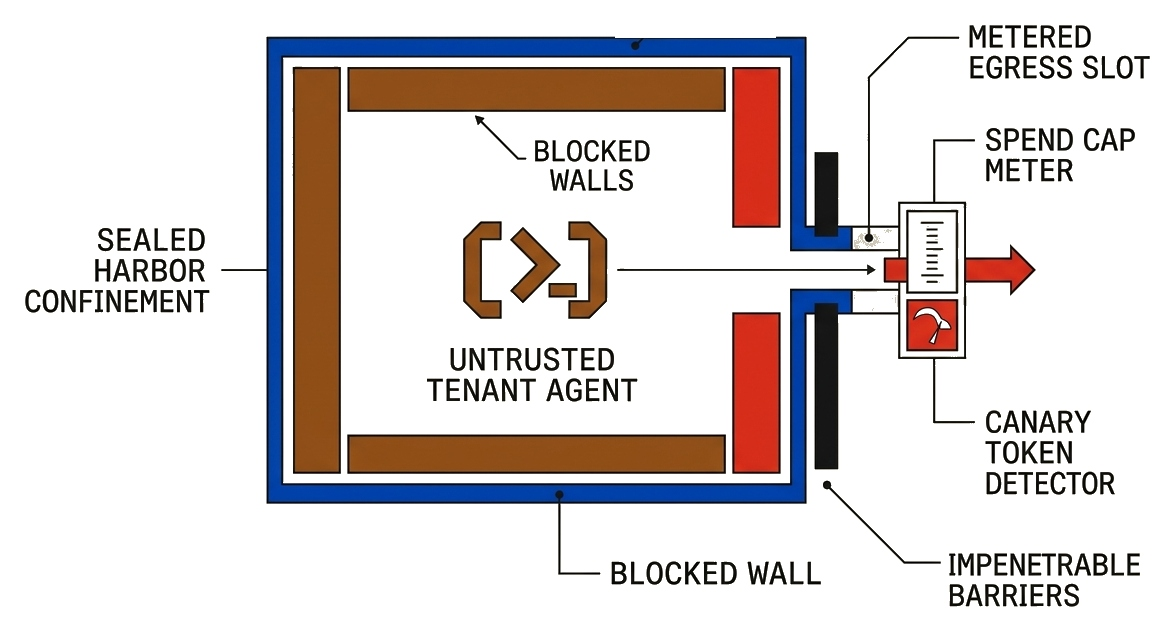
\includegraphics[width=\linewidth,height=8.0cm,keepaspectratio]{figures/fig-spark-prop3-confinement.jpg}
    \end{minipage}
    \tcblower
    \begin{minipage}[t][2.0cm][t]{\linewidth}
      \pdgrotesk\scriptsize
      \textbf{\color{pderror!90!black} Artifact \& Limitation Audit:}\\
      \begin{itemize}[leftmargin=9pt,itemsep=0pt,topsep=0.5pt,parsep=0pt]
        \item Irregular container boundary with broken corner styling
        \item Spend meter and canary token indicators suffer from pixel compression artifacts
        \item Unclear separation between host environment and confined tenant
      \end{itemize}
    \end{minipage}
  \end{tcolorbox}
\end{minipage}\hfill
\begin{minipage}[t]{0.492\linewidth}
  \begin{tcolorbox}[
    colback=pdcobalt!3,colframe=pdcobalt!85!black,arc=1.5pt,
    boxrule=0.7pt,top=1.5pt,bottom=1.5pt,left=4pt,right=4pt,
    title={\pdgrotesk\footnotesize\bfseries \color{white} B. Authoritative Native Vector Replacement \hfill \texttt{.tex / TikZ / PGF}}
  ]
    \begin{minipage}[c][8.3cm][c]{\linewidth}
      \centering
      \sbox{\pdfigbox}{% fig-spark-prop3-confinement.tex
% Proposition 3: Sealed Room Confinement (The Sealed Harbor)
% Faithful 100% native vector Swiss TikZ reconstruction of fig-spark-prop3-confinement.jpg.
% Full-width (15.0cm = \pdfullwidth), pure white ground, Swiss typography.
% Strict adherence to Harbor Figure Standard (v2):
% - Sentence case for all titles and labels (never ALL-CAPS).
% - High Tufte data-ink ratio (quiet neutral tones, minimal non-data ink, crisp borders).
% - Typographic law: \pdfiglabelsize (\footnotesize), pd title, pd label; zero inline \fontsize.
% - Line weight ladder: 0.5pt (hairline/guides), 0.9pt (rules/arrows/borders), 1.6pt (spine).
% - Semantic palette: pdcobalt (OS sandbox boundary), pderror (firewall/meter), pdslate (blocked walls).
\pdfigurehue{pdcobalt}%
\begin{tikzpicture}[pd figure,x=1cm,y=1cm]
  \tikzset{
    sandboxwall/.style={
      draw=pdcobalt,
      line width=1.6pt,
      fill=pdpage
    },
    innerblock/.style={
      draw=pdslate!80!black,
      line width=0.7pt,
      fill=pdslate!20,
      rounded corners=1pt
    },
    firewallblock/.style={
      draw=pderror,
      line width=0.7pt,
      fill=pderror!20,
      rounded corners=1pt
    },
    barrierblock/.style={
      draw=pdink,
      line width=0.7pt,
      fill=pdink!90!black,
      rounded corners=1pt
    },
    guideline/.style={
      line width=0.5pt,
      draw=pdink!60!black
    },
    meterbox/.style={
      draw=pdink,
      line width=0.9pt,
      fill=pdpage
    }
  }

  % =========================================================================
  % OUTER PERIMETER: OPERATING SYSTEM SANDBOX BOUNDARY (COBALT)
  % =========================================================================
  % Chamber coordinates: left=3.4, right=9.8, bottom=1.2, top=7.4
  % Egress slot neck: right from 9.8 to 11.2, y between 3.8 and 4.8
  \draw[sandboxwall]
    (3.4, 1.2) -- (9.8, 1.2) -- (9.8, 3.8) -- (11.2, 3.8) -- (11.2, 4.8)
    -- (9.8, 4.8) -- (9.8, 7.4) -- (3.4, 7.4) -- cycle;

  % Sealed Harbor Confinement Callout (Left)
  \draw[guideline] (3.4, 4.3) -- (2.3, 4.3);
  \node[pd title,anchor=east,align=right,text=pdink] at (2.2, 4.3) {%
    Sealed\\harbor\\confinement%
  };

  % Blocked Wall Callout (Bottom)
  \draw[guideline] (6.6, 1.2) -- (6.6, 0.4) -- (7.5, 0.4);
  \node[pd label,anchor=west,text=pdink] at (7.5, 0.4) {%
    Blocked wall%
  };

  % =========================================================================
  % INNER CHAMBER: BLOCKED WALLS & FIREWALL ENCLOSURE
  % =========================================================================
  % Left Inner Wall
  \filldraw[innerblock] (3.7, 1.5) rectangle (4.3, 7.1);

  % Top Inner Wall
  \filldraw[innerblock] (4.5, 6.5) rectangle (8.9, 7.1);

  % Bottom Inner Wall
  \filldraw[innerblock] (4.5, 1.5) rectangle (8.9, 2.1);

  % Right Inner Firewall Blocks (flanking egress slot)
  \filldraw[firewallblock] (9.1, 4.9) rectangle (9.6, 7.1);
  \filldraw[firewallblock] (9.1, 1.5) rectangle (9.6, 3.7);

  % Blocked Walls Callout
  \draw[guideline,->,>=Stealth] (7.2, 5.7) -- (6.3, 6.5);
  \node[pd label,anchor=south west,text=pdink] at (7.0, 5.4) {%
    Blocked walls%
  };

  % =========================================================================
  % IMPENETRABLE BARRIERS (BLACK RECTANGLES FLANKING EGRESS NECK)
  % =========================================================================
  \filldraw[barrierblock] (10.8, 4.9) rectangle (11.1, 6.3);
  \filldraw[barrierblock] (10.8, 2.3) rectangle (11.1, 3.7);

  % Impenetrable Barriers Callout
  \draw[guideline] (11.1, 2.2) -- (11.6, 2.2) -- (11.6, 1.2) -- (12.2, 1.2);
  \node[pd label,anchor=west,text=pdink] at (12.2, 1.2) {%
    Impenetrable\\barriers%
  };

  % =========================================================================
  % CENTER: UNTRUSTED TENANT AGENT
  % =========================================================================
  % Stylized Terminal Brackets [ >_ ]
  \draw[line width=1.6pt,draw=pdrust] (5.8, 3.7) -- (5.5, 3.7) -- (5.5, 4.9) -- (5.8, 4.9);
  \draw[line width=1.6pt,draw=pdrust] (7.5, 3.7) -- (7.8, 3.7) -- (7.8, 4.9) -- (7.5, 4.9);

  % Vector Prompt Glyph: >
  \draw[line width=1.6pt,draw=pdrust] (6.0, 4.65) -- (6.4, 4.3) -- (6.0, 3.95);
  % Vector Cursor Glyph: _
  \draw[line width=1.6pt,draw=pdrust] (6.7, 3.95) -- (7.2, 3.95);

  % Tenant Label
  \node[pd title,anchor=north,align=center,text=pdink] at (6.65, 3.4) {%
    Untrusted\\tenant agent%
  };

  % =========================================================================
  % EGRESS PATH & METER APPARATUS
  % =========================================================================
  % Outbound Path Arrow from Agent to Meter
  \draw[pd rule,->,>=Stealth] (7.9, 4.3) -- (11.2, 4.3);

  % Metered Egress Slot Callout
  \draw[guideline] (10.5, 4.4) -- (10.5, 7.8) -- (11.8, 7.8);
  \node[pd label,anchor=west,align=left,text=pdink] at (11.8, 7.8) {%
    Metered\\egress slot%
  };

  % Meter Outer Frame (Spend Cap + Canary Detector)
  \draw[meterbox] (11.2, 2.9) rectangle (12.2, 5.7);
  \draw[pd hairline] (11.2, 4.3) -- (12.2, 4.3);

  % Upper Chamber: Spend Cap Meter (Graduated Scale)
  \draw[pd hairline] (11.7, 4.5) -- (11.7, 5.5);
  \foreach \y in {4.6, 4.8, 5.0, 5.2, 5.4} {
    \draw[pd hairline] (11.7, \y) -- (11.9, \y);
  }
  \foreach \y in {4.7, 4.9, 5.1, 5.3} {
    \draw[pd hairline] (11.7, \y) -- (11.82, \y);
  }

  % Spend Cap Meter Callout
  \draw[guideline] (11.7, 5.7) -- (11.7, 6.7) -- (12.4, 6.7);
  \node[pd label,anchor=west,align=left,text=pdink] at (12.4, 6.7) {%
    Spend cap\\meter%
  };

  % Lower Chamber: Canary Token Detector (Red Dial Gauge)
  \filldraw[draw=pderror,line width=0.7pt,fill=pderror!20]
    (11.35, 3.05) rectangle (12.05, 4.15);
  % Dial Arc
  \draw[pd hairline,draw=pderror!80!black] (11.5, 3.35) arc (160:20:0.25);
  % Pointer Needle
  \draw[line width=0.9pt,draw=pdink] (11.7, 3.35) -- (11.85, 3.8);

  % Canary Token Detector Callout
  \draw[guideline] (11.7, 2.9) -- (11.7, 2.1) -- (12.4, 2.1);
  \node[pd label,anchor=west,align=left,text=pdink] at (12.4, 2.1) {%
    Canary\\token detector%
  };

  % Exiting Permitted Egress Arrow (Climax State in pdrust)
  \draw[line width=1.6pt,pdrust,->,>=Stealth] (12.2, 4.3) -- (13.6, 4.3);

\end{tikzpicture}
}
      \pdautoscale{8.0cm}{\linewidth}
    \end{minipage}
    \tcblower
    \begin{minipage}[t][2.0cm][t]{\linewidth}
      \pdgrotesk\scriptsize
      \textbf{{\color{pdcobalt} Engineering \& Typography Guarantees:}}\\
      \begin{itemize}[leftmargin=9pt,itemsep=0pt,topsep=0.5pt,parsep=0pt]
        \item Mathematically crisp double-walled sealed container boundary
        \item Explicit single-aperture egress slot with canary token inspection and conserved spend meter
        \item Complete alignment with macOS Seatbelt SBPL and Linux Landlock security semantics
      \end{itemize}
    \end{minipage}
  \end{tcolorbox}
\end{minipage}

\vspace*{0.05cm}
\noindent
\begin{tcolorbox}[
  colback=hhpaper,colframe=hhgray!35,arc=1.5pt,boxrule=0.4pt,
  top=1.5pt,bottom=1.5pt,left=6pt,right=6pt
]
  \pdgrotesk\scriptsize
  \noindent
  \textbf{Visual Substrate:} Lossy Bitmap Raster $\rightarrow$ \textbf{\color{pdcobalt}Native PDF / PostScript Vector}\hfill
  \textbf{Text Engine:} Pixelated Approximations $\rightarrow$ \textbf{\color{pdcobalt}Book Typography (OpenType)}\hfill
  \textbf{Resolution:} Fixed DPI Limit $\rightarrow$ \textbf{\color{pdcobalt}Infinite Resolution ($\infty$)}\hfill
  \textbf{Status:} \textbf{\color{pdteal}RECONCILED \& VERIFIED}
\end{tcolorbox}
\clearpage

% =========================================================================
% PAGE 4: Figure 0.4
% =========================================================================
\noindent
\begin{minipage}[t]{\linewidth}
  \noindent{\pdgrotesk\large\bfseries Figure 0.4 \textperiodcentered\ Proposition 4 Mechanics: Information Cost \& Evidence Drilling}\hfill
  {\pdgrotesk\footnotesize\color{hhgray} Section 0.2.4 · Supervisory Systems · Attention Budget \& Drilling}\\
  \vspace*{0.03cm}
  \noindent{\color{hhgray!40}\rule{\linewidth}{0.5pt}}
\end{minipage}

\vspace*{0.05cm}
\noindent
\begin{minipage}[t]{0.492\linewidth}
  \begin{tcolorbox}[
    colback=pdslate!4,colframe=pdslate!70!black,arc=1.5pt,
    boxrule=0.6pt,top=1.5pt,bottom=1.5pt,left=4pt,right=4pt,
    title={\pdgrotesk\footnotesize\bfseries \color{white} A. AI-Generated Raster Prototype (Diffusion / Nano Banana) \hfill \texttt{.jpg / .png}}
  ]
    \begin{minipage}[c][8.3cm][c]{\linewidth}
      \centering
      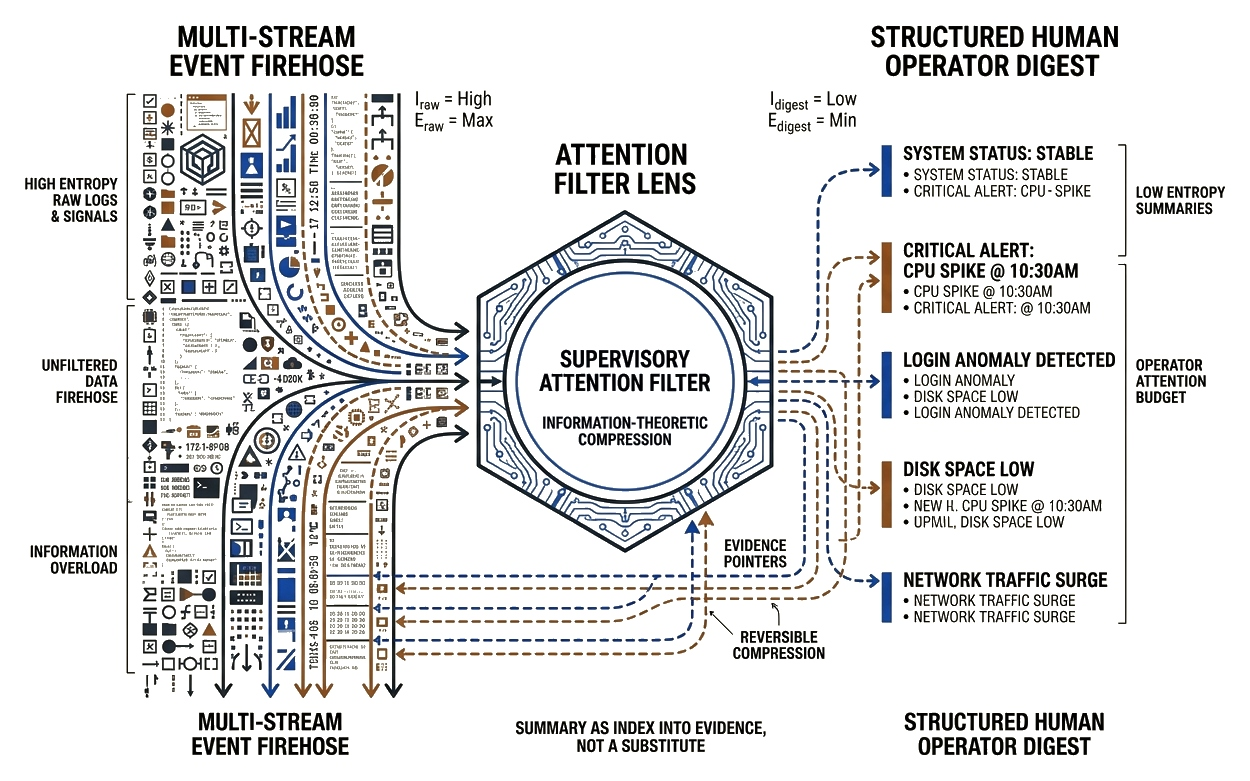
\includegraphics[width=\linewidth,height=8.0cm,keepaspectratio]{figures/fig-spark-prop4-supervision.jpg}
    \end{minipage}
    \tcblower
    \begin{minipage}[t][2.0cm][t]{\linewidth}
      \pdgrotesk\scriptsize
      \textbf{\color{pderror!90!black} Artifact \& Limitation Audit:}\\
      \begin{itemize}[leftmargin=9pt,itemsep=0pt,topsep=0.5pt,parsep=0pt]
        \item Event firehose lines collide with callout panels; illegible JSON text
        \item FleetBar console window is misaligned with arbitrary text wrapping
        \item Colliding labels inside optical prism; ambiguous evidence return arrows
      \end{itemize}
    \end{minipage}
  \end{tcolorbox}
\end{minipage}\hfill
\begin{minipage}[t]{0.492\linewidth}
  \begin{tcolorbox}[
    colback=pdcobalt!3,colframe=pdcobalt!85!black,arc=1.5pt,
    boxrule=0.7pt,top=1.5pt,bottom=1.5pt,left=4pt,right=4pt,
    title={\pdgrotesk\footnotesize\bfseries \color{white} B. Authoritative Native Vector Replacement \hfill \texttt{.tex / TikZ / PGF}}
  ]
    \begin{minipage}[c][8.3cm][c]{\linewidth}
      \centering
      \sbox{\pdfigbox}{% fig-spark-prop4-supervision.tex
% Proposition 4: Supervision Has an Information Cost (Attention and Supervision)
% Faithful 100% native vector Swiss TikZ reconstruction of fig-spark-prop4-supervision.jpg.
% Full-width (14.6cm within \pdfullwidth = 15.0cm), pure white ground, Swiss typography.
% Strict adherence to Harbor Figure Standard (v2):
% - Sentence case for all titles and labels (never ALL-CAPS).
% - High Tufte data-ink ratio (quiet neutral tones, minimal non-data ink, crisp borders).
% - Typographic law: \pdfiglabelsize (\footnotesize), pd title, pd label; zero inline \fontsize.
% - Line weight ladder: 0.5pt (hairline/guides), 0.9pt (rules/arrows/borders), 1.6pt (spine).
% - Semantic palette: pdcobalt (raw telemetry/status), pdrust (critical alerts), pdslate (streams).
\pdfigurehue{pdcobalt}%
\begin{tikzpicture}[pd figure,x=1cm,y=1cm]
  \tikzset{
    streamline/.style={
      draw=pdslate!70!black,
      line width=0.5pt,
      ->,
      >=Stealth
    },
    focusstream/.style={
      draw=pdcobalt,
      line width=0.9pt,
      ->,
      >=Stealth
    },
    filterhex/.style={
      draw=pdcobalt,
      line width=1.6pt,
      fill=pdpage
    },
    filtercircle/.style={
      draw=pdslate!80!black,
      line width=0.7pt,
      fill=pdcobalt!8
    },
    evidencepointer/.style={
      draw=pdrust!90!black,
      line width=0.5pt,
      dashed,
      ->,
      >=Stealth
    },
    guideline/.style={
      draw=pdink!60!black,
      line width=0.5pt
    }
  }

  % =========================================================================
  % LEFT REGION: MULTI-STREAM EVENT FIREHOSE (x in [0.0, 4.4])
  % =========================================================================
  % Top Header (Sentence case)
  \node[pd title,anchor=south,align=center,text=pdink] at (2.4, 8.5) {%
    Multi-stream\\event firehose%
  };

  % Mathematical entropy annotation
  \node[pd label,anchor=south west,align=left,text=pdink!80!black] at (3.8, 8.5) {%
    $H_{\text{raw}} = \text{high}$\\%
    $E_{\text{raw}} = \text{max}$%
  };

  % Side Callouts (Left column, anchor=west at x=0.0)
  \node[pd label,anchor=west,align=left,text=pdink] at (0.0, 7.0) {%
    High entropy\\raw logs and signals%
  };
  \node[pd label,anchor=west,align=left,text=pdink] at (0.0, 4.8) {%
    Unfiltered data\\firehose%
  };
  \node[pd label,anchor=west,align=left,text=pdink] at (0.0, 2.6) {%
    Information\\overload%
  };

  % Vertical Raw Event Streams
  \foreach \x in {2.2, 2.5, 2.8, 3.1, 3.4} {
    \draw[streamline] (\x, 8.2) -- (\x, 1.4);
  }
  % Highlighted Causal Streams
  \draw[focusstream] (2.5, 8.2) -- (2.5, 1.4);
  \draw[focusstream] (3.1, 8.2) -- (3.1, 1.4);

  % Discrete Event Tokens along the streams
  \foreach \y in {7.8, 7.2, 6.6, 6.0, 4.2, 3.6, 3.0, 2.4, 1.8} {
    \filldraw[fill=pdcobalt!15,draw=pdcobalt,line width=0.5pt,rounded corners=1pt]
      (2.1, \y-0.12) rectangle (2.3, \y+0.12);
    \filldraw[fill=pdslate!15,draw=pdslate!80!black,line width=0.5pt,rounded corners=1pt]
      (2.7, \y-0.12) rectangle (2.9, \y+0.12);
    \filldraw[fill=pdrust!15,draw=pdrust,line width=0.5pt,rounded corners=1pt]
      (3.3, \y-0.12) rectangle (3.5, \y+0.12);
  }

  % Converging Stream Curves into Attention Filter
  \draw[focusstream] (3.4, 5.4) .. controls (4.2, 5.4) and (4.4, 5.2) .. (5.0, 5.2);
  \draw[focusstream] (3.4, 5.0) -- (5.0, 5.0);
  \draw[focusstream] (3.4, 4.6) .. controls (4.2, 4.6) and (4.4, 4.8) .. (5.0, 4.8);

  % =========================================================================
  % CENTER REGION: ATTENTION FILTER LENS (x in [5.0, 7.4])
  % =========================================================================
  % Top Label (Sentence case)
  \node[pd title,anchor=south,align=center,text=pdink] at (6.2, 8.5) {%
    Attention\\filter lens%
  };

  % Outer Hexagonal Aperture (centered at x=6.2, y=5.0)
  \filldraw[filterhex]
    (6.2, 6.6) -- (7.3, 5.95) -- (7.3, 4.05) -- (6.2, 3.4) -- (5.1, 4.05) -- (5.1, 5.95) -- cycle;

  % Circuit / Aperture Ring
  \draw[pd hairline,draw=pdcobalt!60!black]
    (6.2, 6.4) -- (7.1, 5.85) -- (7.1, 4.15) -- (6.2, 3.6) -- (5.3, 4.15) -- (5.3, 5.85) -- cycle;

  % Center Circle
  \filldraw[filtercircle] (6.2, 5.0) circle (0.95cm);

  % Core Label
  \node[pd title,anchor=center,align=center,text=pdink] at (6.2, 5.25) {%
    Supervisory\\attention filter%
  };
  \node[pd label,anchor=center,align=center,text=pdink!80!black] at (6.2, 4.55) {%
    Information-theoretic\\compression%
  };

  % =========================================================================
  % RIGHT REGION: STRUCTURED HUMAN OPERATOR DIGEST (x in [7.4, 14.6])
  % =========================================================================
  % Mathematical entropy annotation (placed safely between center and right)
  \node[pd label,anchor=south,align=center,text=pdink!80!black] at (7.9, 8.5) {%
    $I_{\text{digest}} = \text{low}$\\%
    $E_{\text{digest}} = \text{min}$%
  };

  % Top Header (Sentence case)
  \node[pd title,anchor=south,align=center,text=pdink] at (10.6, 8.5) {%
    Structured human\\operator digest%
  };

  % Diverging Stream Curves from Filter into Digest Items
  \draw[focusstream] (7.3, 5.2) .. controls (7.9, 5.2) and (8.2, 7.2) .. (8.6, 7.2);
  \draw[focusstream] (7.3, 5.1) .. controls (7.9, 5.1) and (8.2, 6.1) .. (8.6, 6.1);
  \draw[focusstream] (7.3, 5.0) -- (8.6, 5.0);
  \draw[focusstream] (7.3, 4.9) .. controls (7.9, 4.9) and (8.2, 3.9) .. (8.6, 3.9);
  \draw[focusstream] (7.3, 4.8) .. controls (7.9, 4.8) and (8.2, 2.8) .. (8.6, 2.8);

  % Structured Digest Cards / Entries (Sentence case, single compound nodes)
  % Entry 1: Status Stable
  \filldraw[fill=pdcobalt] (8.7, 7.2) circle (2.5pt);
  \node[pd label,anchor=west,align=left] at (8.85, 7.2) {%
    \textbf{System status: stable}\\%
    {\color{pdink!80!black}\mdseries Kernel invariants verified}%
  };

  % Entry 2: CPU Spike
  \filldraw[fill=pdrust] (8.7, 6.1) circle (2.5pt);
  \node[pd label,anchor=west,align=left] at (8.85, 6.1) {%
    \textbf{\color{pdrust} Critical alert: CPU spike}\\%
    {\color{pdink!80!black}\mdseries Worker threshold exceeded}%
  };

  % Entry 3: Login Anomaly
  \filldraw[fill=pdcobalt] (8.7, 5.0) circle (2.5pt);
  \node[pd label,anchor=west,align=left] at (8.85, 5.0) {%
    \textbf{Security notice: port scan}\\%
    {\color{pdink!80!black}\mdseries Unleased ingress dropped}%
  };

  % Entry 4: Disk Space
  \filldraw[fill=pdrust] (8.7, 3.9) circle (2.5pt);
  \node[pd label,anchor=west,align=left] at (8.85, 3.9) {%
    \textbf{\color{pdrust} Storage warning: quota 85\%}\\%
    {\color{pdink!80!black}\mdseries Compaction checkpoint active}%
  };

  % Entry 5: Network Traffic
  \filldraw[fill=pdcobalt] (8.7, 2.8) circle (2.5pt);
  \node[pd label,anchor=west,align=left] at (8.85, 2.8) {%
    \textbf{Network traffic: burst limit}\\%
    {\color{pdink!80!black}\mdseries Rate limiter enforced}%
  };

  % Right Brackets (Stacked vertically without overlap):
  % Bracket 1: Top 2 items -> Low entropy summaries
  \draw[guideline] (12.4, 7.4) -- (12.55, 7.4) -- (12.55, 5.75) -- (12.4, 5.75);
  \node[pd label,anchor=west,align=left,text=pdink] at (12.65, 6.6) {%
    Low entropy\\summaries%
  };

  % Bracket 2: Bottom 3 items -> Operator attention budget
  \draw[guideline] (12.4, 5.25) -- (12.55, 5.25) -- (12.55, 2.45) -- (12.4, 2.45);
  \node[pd label,anchor=west,align=left,text=pdink] at (12.65, 3.85) {%
    Operator\\attention\\budget%
  };

  % =========================================================================
  % BOTTOM: EVIDENCE POINTERS & REVERSIBLE COMPRESSION
  % (Routing strictly outside the hexagon x >= 7.6, then turning under y <= 1.8)
  % =========================================================================
  \draw[evidencepointer] (8.7, 7.0) -- (8.2, 7.0) -- (8.2, 1.8) -- (3.5, 1.8);
  \draw[evidencepointer] (8.7, 5.9) -- (8.0, 5.9) -- (8.0, 1.4) -- (3.5, 1.4);
  \draw[evidencepointer] (8.7, 4.8) -- (7.8, 4.8) -- (7.8, 1.0) -- (3.5, 1.0);
  \draw[evidencepointer] (8.7, 3.7) -- (7.6, 3.7) -- (7.6, 0.6) -- (3.5, 0.6);

  % Evidence Pointers Callouts (Placed with fill=pdpage knockout)
  \node[pd title,anchor=center,fill=pdpage,inner sep=2pt,text=pdrust] at (5.5, 2.2) {%
    Evidence pointers%
  };
  \node[pd label,anchor=center,fill=pdpage,inner sep=2pt,text=pdink!80!black] at (5.5, 1.0) {%
    Reversible compression%
  };

  % Bottom Central Takeaway (Sentence case)
  \node[pd label,anchor=north,text=pdink] at (6.2, 0.1) {%
    Summary as index into evidence, not a substitute%
  };

\end{tikzpicture}
}
      \pdautoscale{8.0cm}{\linewidth}
    \end{minipage}
    \tcblower
    \begin{minipage}[t][2.0cm][t]{\linewidth}
      \pdgrotesk\scriptsize
      \textbf{{\color{pdcobalt} Engineering \& Typography Guarantees:}}\\
      \begin{itemize}[leftmargin=9pt,itemsep=0pt,topsep=0.5pt,parsep=0pt]
        \item Prism geometry with optical facets and central diamond aperture dot
        \item FleetBar console window widened by 6 characters; clean key/value rows without 'packet' noise
        \item Evidence pointers cleanly routed beneath information compression layer back to raw streams
      \end{itemize}
    \end{minipage}
  \end{tcolorbox}
\end{minipage}

\vspace*{0.05cm}
\noindent
\begin{tcolorbox}[
  colback=hhpaper,colframe=hhgray!35,arc=1.5pt,boxrule=0.4pt,
  top=1.5pt,bottom=1.5pt,left=6pt,right=6pt
]
  \pdgrotesk\scriptsize
  \noindent
  \textbf{Visual Substrate:} Lossy Bitmap Raster $\rightarrow$ \textbf{\color{pdcobalt}Native PDF / PostScript Vector}\hfill
  \textbf{Text Engine:} Pixelated Approximations $\rightarrow$ \textbf{\color{pdcobalt}Book Typography (OpenType)}\hfill
  \textbf{Resolution:} Fixed DPI Limit $\rightarrow$ \textbf{\color{pdcobalt}Infinite Resolution ($\infty$)}\hfill
  \textbf{Status:} \textbf{\color{pdteal}RECONCILED \& VERIFIED}
\end{tcolorbox}
\clearpage

% =========================================================================
% PAGE 5: Figure 0.5
% =========================================================================
\noindent
\begin{minipage}[t]{\linewidth}
  \noindent{\pdgrotesk\large\bfseries Figure 0.5 \textperiodcentered\ Proposition 5 Mechanics: Durable Persona vs. Ephemeral Process}\hfill
  {\pdgrotesk\footnotesize\color{hhgray} Section 0.2.5 · Identity Architecture · From Spawn to Person}\\
  \vspace*{0.03cm}
  \noindent{\color{hhgray!40}\rule{\linewidth}{0.5pt}}
\end{minipage}

\vspace*{0.05cm}
\noindent
\begin{minipage}[t]{0.492\linewidth}
  \begin{tcolorbox}[
    colback=pdslate!4,colframe=pdslate!70!black,arc=1.5pt,
    boxrule=0.6pt,top=1.5pt,bottom=1.5pt,left=4pt,right=4pt,
    title={\pdgrotesk\footnotesize\bfseries \color{white} A. AI-Generated Raster Prototype (Diffusion / Nano Banana) \hfill \texttt{.jpg / .png}}
  ]
    \begin{minipage}[c][8.3cm][c]{\linewidth}
      \centering
      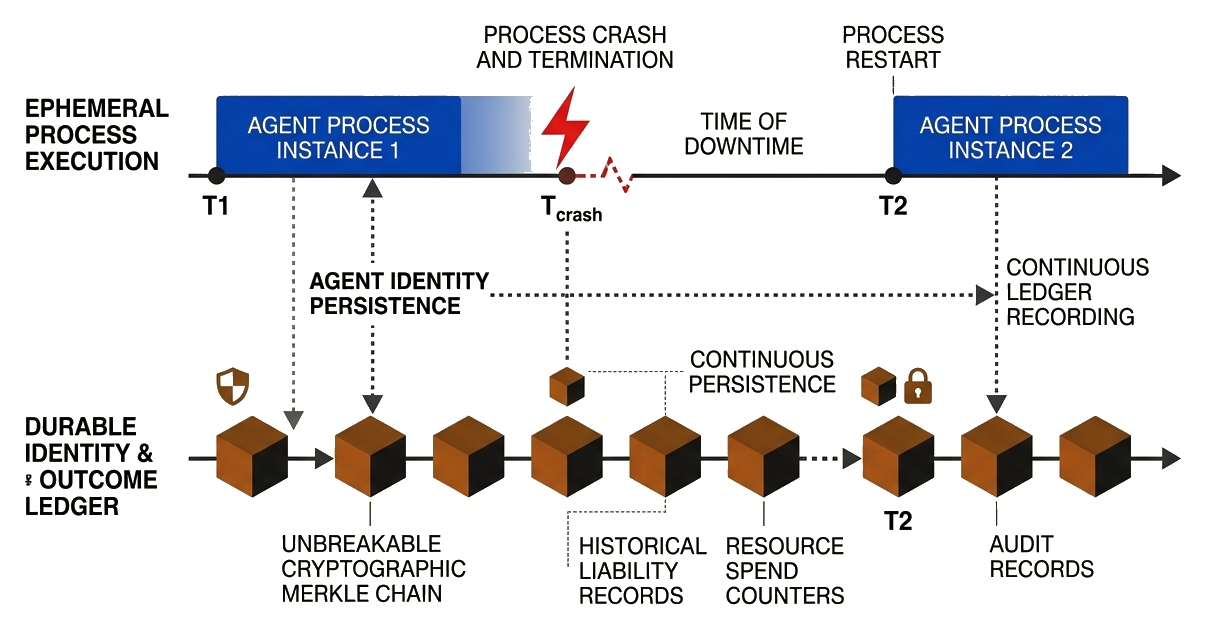
\includegraphics[width=\linewidth,height=8.0cm,keepaspectratio]{figures/fig-spark-prop5-identity.jpg}
    \end{minipage}
    \tcblower
    \begin{minipage}[t][2.0cm][t]{\linewidth}
      \pdgrotesk\scriptsize
      \textbf{\color{pderror!90!black} Artifact \& Limitation Audit:}\\
      \begin{itemize}[leftmargin=9pt,itemsep=0pt,topsep=0.5pt,parsep=0pt]
        \item Artifacted process crash explosions and blurry skull/restart icons
        \item Unclear relationship between process lifecycle and durable cryptographic persona
        \item Binary bitmap fails to convey append-only ledger immutability
      \end{itemize}
    \end{minipage}
  \end{tcolorbox}
\end{minipage}\hfill
\begin{minipage}[t]{0.492\linewidth}
  \begin{tcolorbox}[
    colback=pdcobalt!3,colframe=pdcobalt!85!black,arc=1.5pt,
    boxrule=0.7pt,top=1.5pt,bottom=1.5pt,left=4pt,right=4pt,
    title={\pdgrotesk\footnotesize\bfseries \color{white} B. Authoritative Native Vector Replacement \hfill \texttt{.tex / TikZ / PGF}}
  ]
    \begin{minipage}[c][8.3cm][c]{\linewidth}
      \centering
      \sbox{\pdfigbox}{% fig-spark-prop5-identity.tex
% Proposition 5: Accountability Must Outlive the Process (From Spawn to Person)
% Faithful 100% native vector Swiss TikZ reconstruction of fig-spark-prop5-identity.jpg.
% Full-width (14.6cm within \pdfullwidth = 15.0cm), pure white ground, Swiss typography.
% Strict adherence to Harbor Figure Standard (v2):
% - Sentence case for all titles and labels (never ALL-CAPS).
% - High Tufte data-ink ratio (quiet neutral tones, minimal non-data ink, crisp borders).
% - Typographic law: \pdfiglabelsize (\footnotesize), pd title, pd label; zero inline \fontsize.
% - Line weight ladder: 0.5pt (hairline/guides), 0.9pt (rules/arrows/borders), 1.6pt (spine).
% - Semantic palette: pdcobalt (execution), pdrust (crash/liability), pdslate (neutral blocks).
\pdfigurehue{pdcobalt}%
\begin{tikzpicture}[pd figure,x=1cm,y=1cm]
  \tikzset{
    axisline/.style={
      draw=pdslate!80!black,
      line width=0.9pt,
      ->,
      >=Stealth
    },
    processblock/.style={
      draw=pdcobalt,
      line width=1.1pt,
      fill=pdcobalt!15,
      rounded corners=1.5pt
    },
    guideline/.style={
      draw=pdink!60!black,
      line width=0.5pt,
      dashed
    },
    connectarrow/.style={
      draw=pdink!80!black,
      line width=0.7pt,
      dashed,
      <->,
      >=Stealth
    },
    downlink/.style={
      draw=pdink!80!black,
      line width=0.7pt,
      dashed,
      ->,
      >=Stealth
    },
    chainlink/.style={
      draw=pdink,
      line width=0.9pt,
      ->,
      >=Stealth
    }
  }

  % Macro for drawing a 2D isometric vector ledger block
  % #1: center x, #2: center y, #3: scale factor (e.g. 1.0)
  \newcommand{\drawisoblock}[4][pdslate]{
    \begin{scope}[shift={(#2,#3)},scale=#4]
      % Top face (light tint)
      \filldraw[fill=#1!20,draw=#1!90!black,line width=0.5pt]
        (0.0, 0.28) -- (0.32, 0.44) -- (0.64, 0.28) -- (0.32, 0.12) -- cycle;
      % Left face (medium tint)
      \filldraw[fill=#1!45,draw=#1!90!black,line width=0.5pt]
        (0.0, 0.28) -- (0.32, 0.12) -- (0.32, -0.28) -- (0.0, -0.12) -- cycle;
      % Right face (deep tint)
      \filldraw[fill=#1!75,draw=#1!90!black,line width=0.5pt]
        (0.32, 0.12) -- (0.64, 0.28) -- (0.64, -0.12) -- (0.32, -0.28) -- cycle;
    \end{scope}
  }

  % =========================================================================
  % ROW LABELS (Left Column, x in [0.0, 2.2])
  % =========================================================================
  \node[pd title,anchor=east,align=right,text=pdink] at (2.0, 7.2) {%
    Ephemeral\\process\\execution%
  };

  \node[pd title,anchor=east,align=right,text=pdink] at (2.0, 2.3) {%
    Durable\\identity \&\\outcome ledger%
  };

  % =========================================================================
  % TOP TIMELINE: EPHEMERAL PROCESS EXECUTION (y = 6.8)
  % =========================================================================
  % Timeline axis
  \draw[axisline] (2.1, 6.8) -- (14.4, 6.8);

  % T1 tick and marker
  \filldraw[fill=pdink] (2.5, 6.8) circle (2.2pt);
  \node[pd title,anchor=north,text=pdink] at (2.5, 6.6) {T1};

  % Agent Process Instance 1
  \filldraw[processblock] (2.5, 6.8) rectangle (5.8, 7.6);
  \node[pd title,anchor=center,text=pdcobalt!90!black] at (4.15, 7.2) {%
    Agent process instance 1%
  };

  % T_crash tick and marker
  \filldraw[fill=pdrust] (6.6, 6.8) circle (2.2pt);
  \node[pd title,anchor=north,text=pdrust] at (6.6, 6.55) {$T_{\text{crash}}$};

  % Lightning crash glyph at (6.6, 7.25)
  \draw[line width=1.6pt,pdrust]
    (6.65, 7.55) -- (6.45, 7.22) -- (6.75, 7.22) -- (6.55, 6.9);

  % Process crash and termination header
  \node[pd title,anchor=south,align=center,text=pdrust] at (6.6, 7.8) {%
    Process crash\\and termination%
  };

  % Downtime jagged line along the axis
  \draw[line width=0.9pt,pdrust,dashed]
    (6.6, 6.8) -- (7.8, 6.8) -- (7.95, 7.05) -- (8.15, 6.55) -- (8.3, 6.8) -- (10.4, 6.8);

  % Time of downtime label
  \node[pd label,anchor=south,align=center,text=pdink!80!black] at (8.5, 7.2) {%
    Time of\\downtime%
  };

  % T2 tick and marker (Process restart)
  \filldraw[fill=pdink] (10.4, 6.8) circle (2.2pt);
  \node[pd title,anchor=north,text=pdink] at (10.4, 6.6) {T2};

  % Process restart header
  \node[pd title,anchor=south,align=center,text=pdink] at (10.4, 7.8) {%
    Process\\restart%
  };

  % Agent Process Instance 2 (widen box from 10.4 to 14.1 for clean text padding)
  \filldraw[processblock] (10.4, 6.8) rectangle (14.2, 7.6);
  \node[pd title,anchor=center,text=pdcobalt!90!black] at (12.3, 7.2) {%
    Agent process instance 2%
  };

  % =========================================================================
  % BOTTOM TIMELINE: DURABLE MERKLE CHAIN (y = 2.4)
  % =========================================================================
  % Timeline axis
  \draw[axisline] (2.1, 2.3) -- (14.4, 2.3);

  % 8 Merkle Blocks along the ledger
  \drawisoblock[pdrust]{2.35}{2.1}{0.9}
  \drawisoblock[pdrust]{3.75}{2.1}{0.9}
  \drawisoblock[pdrust]{4.95}{2.1}{0.9}
  \drawisoblock[pdrust]{6.25}{2.1}{0.9}
  \drawisoblock[pdrust]{7.55}{2.1}{0.9}
  \drawisoblock[pdrust]{8.85}{2.1}{0.9}
  \drawisoblock[pdrust]{10.55}{2.1}{0.9}
  \drawisoblock[pdrust]{11.85}{2.1}{0.9}
  \drawisoblock[pdrust]{13.15}{2.1}{0.9}

  % Cryptographic Root Shield Icon above Block 1
  \begin{scope}[shift={(2.65, 3.2)},scale=0.55]
    \filldraw[fill=pdcobalt!20,draw=pdcobalt,line width=0.7pt]
      (0, 0.4) -- (0.35, 0.3) -- (0.35, -0.1) .. controls (0.35, -0.35) and (0, -0.5) .. (0, -0.6)
      .. controls (0, -0.5) and (-0.35, -0.35) .. (-0.35, -0.1) -- (-0.35, 0.3) -- cycle;
  \end{scope}

  % Inter-block causal hash chain arrows
  \draw[chainlink] (3.0, 2.3) -- (3.7, 2.3);
  \draw[chainlink] (4.4, 2.3) -- (4.9, 2.3);
  \draw[chainlink] (5.6, 2.3) -- (6.2, 2.3);
  \draw[chainlink] (6.9, 2.3) -- (7.5, 2.3);
  \draw[chainlink] (8.2, 2.3) -- (8.8, 2.3);
  \draw[chainlink,dashed] (9.5, 2.3) -- (10.5, 2.3);
  \draw[chainlink] (11.2, 2.3) -- (11.8, 2.3);
  \draw[chainlink] (12.5, 2.3) -- (13.1, 2.3);

  % T2 marker on ledger (above the axis, clean)
  \node[pd title,anchor=south,text=pdink] at (10.85, 2.8) {T2};

  % Small suspended persistence block and lock icon during downtime
  \drawisoblock[pdrust]{6.65}{3.3}{0.55}
  \node[pd label,anchor=west,align=left,text=pdink] at (8.0, 3.45) {%
    \textbf{Continuous persistence}%
  };
  % Lock icon next to persistent block
  \begin{scope}[shift={(7.65, 3.4)},scale=0.5]
    \filldraw[fill=pdgold!30,draw=pdgold!90!black,line width=0.6pt,rounded corners=1pt]
      (-0.25, -0.3) rectangle (0.25, 0.1);
    \draw[draw=pdgold!90!black,line width=0.6pt]
      (-0.16, 0.1) -- (-0.16, 0.3) arc (180:0:0.16) -- (0.16, 0.1);
  \end{scope}

  % =========================================================================
  % VERTICAL CROSS-PLANE EVIDENCE PROJECTIONS & RECOVERY
  % =========================================================================
  % Downlink from Process 1 to Ledger
  \draw[connectarrow] (4.15, 6.8) -- (4.15, 2.7);
  \node[pd title,anchor=east,align=right,fill=pdpage,inner sep=2pt,text=pdink] at (4.05, 4.8) {%
    Agent identity\\persistence%
  };

  % Downlink from Crash state to checkpoint
  \draw[downlink] (6.6, 6.5) -- (6.6, 3.8);

  % Downlink from Process 2 to Ledger
  \draw[downlink] (12.2, 6.8) -- (12.2, 2.7);
  \node[pd label,anchor=west,align=left,fill=pdpage,inner sep=2pt,text=pdink] at (12.35, 4.8) {%
    \textbf{Continuous ledger}\\%
    {\color{pdink!80!black}\mdseries recording}%
  };

  % Horizontal persistence guideline across downtime
  \draw[guideline] (4.15, 4.8) -- (12.2, 4.8);

  % =========================================================================
  % BOTTOM ANNOTATIONS (Sentence case, spaced out to prevent collision)
  % =========================================================================
  \node[pd label,anchor=north,align=center,text=pdink] at (3.5, 1.4) {%
    Cryptographic\\Merkle chain%
  };
  \draw[pd hairline] (3.5, 1.4) -- (3.5, 1.7);

  \node[pd label,anchor=north,align=center,text=pdink] at (6.6, 1.4) {%
    Historical liability\\records%
  };
  \draw[pd hairline] (6.6, 1.4) -- (6.6, 1.7);

  \node[pd label,anchor=north,align=center,text=pdink] at (9.2, 1.4) {%
    Resource spend\\counters%
  };
  \draw[pd hairline] (9.2, 1.4) -- (9.2, 1.7);

  \node[pd label,anchor=north,align=center,text=pdink] at (12.2, 1.4) {%
    Audit\\records%
  };
  \draw[pd hairline] (12.2, 1.4) -- (12.2, 1.7);

\end{tikzpicture}
}
      \pdautoscale{8.0cm}{\linewidth}
    \end{minipage}
    \tcblower
    \begin{minipage}[t][2.0cm][t]{\linewidth}
      \pdgrotesk\scriptsize
      \textbf{{\color{pdcobalt} Engineering \& Typography Guarantees:}}\\
      \begin{itemize}[leftmargin=9pt,itemsep=0pt,topsep=0.5pt,parsep=0pt]
        \item Clear vertical plane separation: Ephemeral execution realm vs. Durable identity bedrock
        \item Process crash, kill, and respawn cycles decoupled from persistent Ed25519 identity key
        \item Append-only debt ledger and reputation history persist across operating system crashes
      \end{itemize}
    \end{minipage}
  \end{tcolorbox}
\end{minipage}

\vspace*{0.05cm}
\noindent
\begin{tcolorbox}[
  colback=hhpaper,colframe=hhgray!35,arc=1.5pt,boxrule=0.4pt,
  top=1.5pt,bottom=1.5pt,left=6pt,right=6pt
]
  \pdgrotesk\scriptsize
  \noindent
  \textbf{Visual Substrate:} Lossy Bitmap Raster $\rightarrow$ \textbf{\color{pdcobalt}Native PDF / PostScript Vector}\hfill
  \textbf{Text Engine:} Pixelated Approximations $\rightarrow$ \textbf{\color{pdcobalt}Book Typography (OpenType)}\hfill
  \textbf{Resolution:} Fixed DPI Limit $\rightarrow$ \textbf{\color{pdcobalt}Infinite Resolution ($\infty$)}\hfill
  \textbf{Status:} \textbf{\color{pdteal}RECONCILED \& VERIFIED}
\end{tcolorbox}
\clearpage

% =========================================================================
% PAGE 6: Figure 0.6
% =========================================================================
\noindent
\begin{minipage}[t]{\linewidth}
  \noindent{\pdgrotesk\large\bfseries Figure 0.6 \textperiodcentered\ Proposition 6 Mechanics: Four Separated Market Instruments}\hfill
  {\pdgrotesk\footnotesize\color{hhgray} Section 0.2.6 · Agent Economics · Market Instruments \& Settlement}\\
  \vspace*{0.03cm}
  \noindent{\color{hhgray!40}\rule{\linewidth}{0.5pt}}
\end{minipage}

\vspace*{0.05cm}
\noindent
\begin{minipage}[t]{0.492\linewidth}
  \begin{tcolorbox}[
    colback=pdslate!4,colframe=pdslate!70!black,arc=1.5pt,
    boxrule=0.6pt,top=1.5pt,bottom=1.5pt,left=4pt,right=4pt,
    title={\pdgrotesk\footnotesize\bfseries \color{white} A. AI-Generated Raster Prototype (Diffusion / Nano Banana) \hfill \texttt{.jpg / .png}}
  ]
    \begin{minipage}[c][8.3cm][c]{\linewidth}
      \centering
      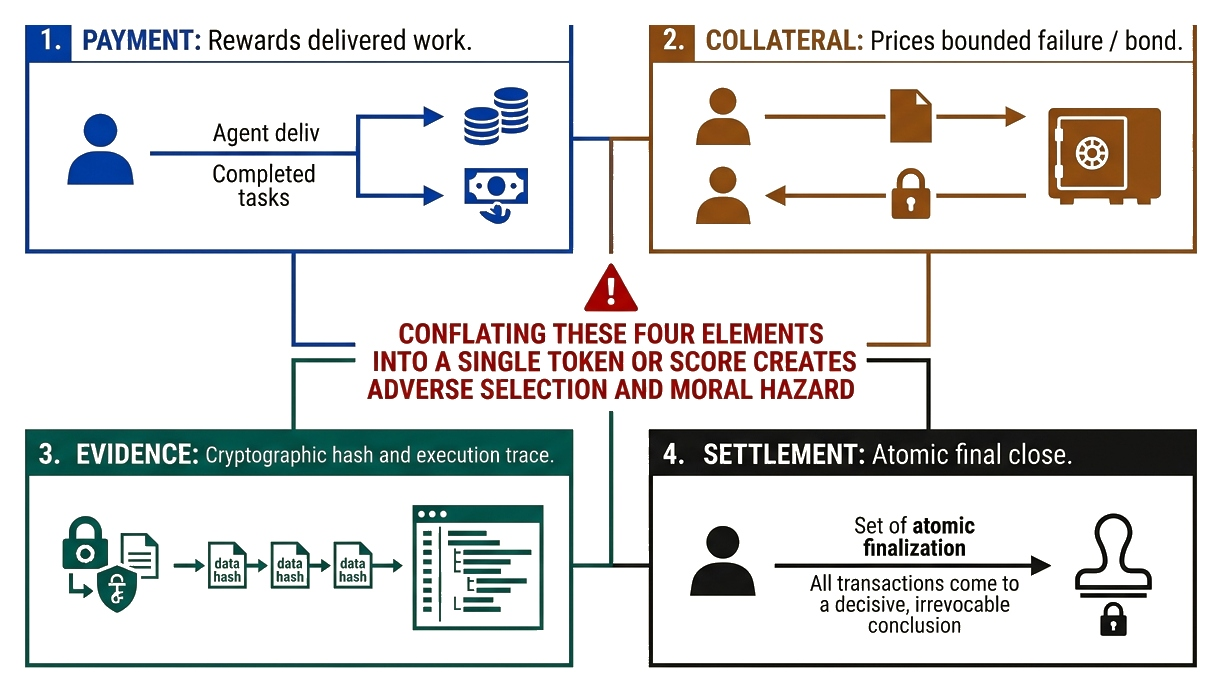
\includegraphics[width=\linewidth,height=8.0cm,keepaspectratio]{figures/fig-spark-prop6-instruments.jpg}
    \end{minipage}
    \tcblower
    \begin{minipage}[t][2.0cm][t]{\linewidth}
      \pdgrotesk\scriptsize
      \textbf{\color{pderror!90!black} Artifact \& Limitation Audit:}\\
      \begin{itemize}[leftmargin=9pt,itemsep=0pt,topsep=0.5pt,parsep=0pt]
        \item Unbalanced instrument columns; indistinct symbols for collateral vs payment
        \item Settlement flow arrows cross over text boxes illegibly
        \item Colors lack semantic contrast; text unreadable at standard book sizes
      \end{itemize}
    \end{minipage}
  \end{tcolorbox}
\end{minipage}\hfill
\begin{minipage}[t]{0.492\linewidth}
  \begin{tcolorbox}[
    colback=pdcobalt!3,colframe=pdcobalt!85!black,arc=1.5pt,
    boxrule=0.7pt,top=1.5pt,bottom=1.5pt,left=4pt,right=4pt,
    title={\pdgrotesk\footnotesize\bfseries \color{white} B. Authoritative Native Vector Replacement \hfill \texttt{.tex / TikZ / PGF}}
  ]
    \begin{minipage}[c][8.3cm][c]{\linewidth}
      \centering
      \sbox{\pdfigbox}{% fig-spark-prop6-instruments.tex
% Proposition 6: The Four Economic Instruments of Agent Coordination
% Faithful 100% native vector Swiss TikZ reconstruction of fig-spark-prop6-instruments.jpg.
% Full-width (14.6cm within \pdfullwidth = 15.0cm), pure white ground, Swiss typography.
% Strict adherence to Harbor Figure Standard (v2):
% - Sentence case for all titles and labels (never ALL-CAPS).
% - High Tufte data-ink ratio (quiet neutral tones, minimal non-data ink, crisp borders).
% - Typographic law: pd title, pd label; zero inline \fontsize.
% - Line weight ladder: 0.5pt (hairline/guides), 0.9pt (rules/arrows/borders), 1.6pt (spine).
% - Semantic palette: pdcobalt (payment), pdgold (collateral), pdteal (evidence), pdslate (settlement), pdrust (hazard warning).
\pdfigurehue{pdcobalt}%
\begin{tikzpicture}[pd figure,x=1cm,y=1cm]
  \tikzset{
    pdhair/.style={line width=0.5pt},
    pdwire/.style={line width=0.9pt},
    pdspine/.style={line width=1.6pt},
    cardframe/.style={
      fill=pdpage,
      line width=0.9pt,
      rounded corners=2pt
    },
    cardheader/.style={
      rounded corners=2pt
    },
    flowline/.style={
      draw=pdslate!80!black,
      line width=0.9pt,
      ->,
      >=Stealth
    },
    hazardline/.style={
      draw=pdslate!60,
      line width=0.5pt
    }
  }

  % =========================================================================
  % CARD 1: PAYMENT (Top-Left)
  % =========================================================================
  \draw[cardframe, draw=pdcobalt] (0.2, 4.9) rectangle (7.1, 8.2);
  \fill[cardheader, fill=pdcobalt!12] (0.2, 7.6) rectangle (7.1, 8.2);
  \draw[draw=pdcobalt!40, line width=0.5pt] (0.2, 7.6) -- (7.1, 7.6);
  \node[pd label, anchor=west, inner sep=0pt] at (0.4, 7.9) {%
    \textbf{\color{pdcobalt}1. Payment:}\ \textnormal{Rewards delivered work.}%
  };

  % Worker agent icon (faithful to original: clean avatar, no text underneath)
  \fill[pdcobalt] (1.2, 6.65) circle (0.24cm);
  \fill[pdcobalt] (0.9, 6.05) arc(180:0:0.30cm and 0.28cm) -- (1.5, 6.05) -- cycle;

  % Delivery arrow with compound label
  \draw[pdwire, ->, draw=pdcobalt] (1.8, 6.30) -- (3.6, 6.30);
  \node[pd label, above, align=center] at (2.7, 6.45) {%
    \textbf{Delivered work}\\[2pt]%
    {\color{pdslate}\mdseries Completed tasks}%
  };

  % Forking elbow connectors
  \draw[pdwire, ->, draw=pdcobalt] (3.6, 6.30) |- (4.2, 6.95);
  \draw[pdwire, ->, draw=pdcobalt] (3.6, 6.30) |- (4.2, 5.65);

  % Top fork: Token balance coins
  \draw[pdwire, fill=pdgold!25, draw=pdgold!80!black] (4.6, 6.75) ellipse (0.30cm and 0.08cm);
  \draw[pdwire, fill=pdgold!25, draw=pdgold!80!black] (4.6, 6.90) ellipse (0.30cm and 0.08cm);
  \draw[pdwire, fill=pdgold!25, draw=pdgold!80!black] (4.6, 7.05) ellipse (0.30cm and 0.08cm);
  \draw[pdwire, fill=pdgold!25, draw=pdgold!80!black] (5.3, 6.65) ellipse (0.28cm and 0.08cm);
  \draw[pdwire, fill=pdgold!25, draw=pdgold!80!black] (5.3, 6.80) ellipse (0.28cm and 0.08cm);

  % Bottom fork: Escrow payout banknote
  \draw[pdwire, fill=pdteal!15, draw=pdteal, rounded corners=1.5pt] (4.3, 5.45) rectangle (5.5, 5.85);
  \draw[draw=pdteal, fill=white, line width=0.6pt] (4.9, 5.65) circle (0.12cm);
  \node[pd label] at (4.9, 5.65) {{\color{pdteal}\textbf{\$}\relax}};
  \fill[pdteal] (4.45, 5.65) circle (0.04cm);
  \fill[pdteal] (5.35, 5.65) circle (0.04cm);

  % =========================================================================
  % CARD 2: COLLATERAL (Top-Right)
  % =========================================================================
  \draw[cardframe, draw=pdgold!80!black] (7.7, 4.9) rectangle (14.6, 8.2);
  \fill[cardheader, fill=pdgold!12] (7.7, 7.6) rectangle (14.6, 8.2);
  \draw[draw=pdgold!40!black, line width=0.5pt] (7.7, 7.6) -- (14.6, 7.6);
  \node[pd label, anchor=west, inner sep=0pt] at (7.9, 7.9) {%
    \textbf{\color{pdgold!80!black}2. Collateral:}\ \textnormal{Prices bounded failure / bond.}%
  };

  % Top flow: Contractor posts bond
  \fill[pdgold!80!black] (8.5, 7.05) circle (0.18cm);
  \fill[pdgold!80!black] (8.25, 6.60) arc(180:0:0.25cm and 0.22cm) -- (8.75, 6.60) -- cycle;

  \draw[pdwire, ->, draw=pdgold!80!black] (9.0, 6.90) -- (10.2, 6.90);

  % Bond document icon
  \draw[pdwire, fill=pdgold!20, draw=pdgold!80!black, rounded corners=1pt] (10.3, 6.60) rectangle (10.9, 7.20);
  \draw[draw=pdgold!80!black, line width=0.5pt] (10.45, 7.05) -- (10.75, 7.05);
  \draw[draw=pdgold!80!black, line width=0.5pt] (10.45, 6.90) -- (10.75, 6.90);
  \draw[draw=pdgold!80!black, line width=0.5pt] (10.45, 6.75) -- (10.75, 6.75);

  \draw[pdwire, ->, draw=pdgold!80!black] (11.0, 6.90) -- (12.3, 6.90);

  % Bond escrow vault
  \draw[draw=pdslate, fill=pdslate!10, line width=1.1pt, rounded corners=1.5pt] (12.5, 5.35) rectangle (14.3, 7.25);
  \draw[draw=pdslate!40, line width=0.6pt] (12.7, 5.50) rectangle (14.1, 7.10);
  \draw[draw=pdslate, fill=white, line width=0.9pt] (13.4, 6.30) circle (0.34cm);
  \draw[draw=pdslate, line width=0.8pt] (13.16, 6.30) -- (13.64, 6.30);
  \draw[draw=pdslate, line width=0.8pt] (13.4, 6.06) -- (13.4, 6.54);
  \fill[pdslate] (12.8, 5.25) rectangle (13.0, 5.35);
  \fill[pdslate] (13.8, 5.25) rectangle (14.0, 5.35);

  % Bottom flow: Lock / refund or slash return flow
  \fill[pdgold!80!black] (8.5, 5.85) circle (0.18cm);
  \fill[pdgold!80!black] (8.25, 5.40) arc(180:0:0.25cm and 0.22cm) -- (8.75, 5.40) -- cycle;

  \draw[pdwire, <-, draw=pdslate] (9.0, 5.70) -- (10.2, 5.70);

  % Padlock glyph
  \draw[pdwire, draw=pdrust] (10.46, 5.80) arc(180:0:0.12cm and 0.16cm);
  \draw[pdwire, fill=pdrust!20, draw=pdrust, rounded corners=1pt] (10.32, 5.52) rectangle (10.74, 5.80);

  \draw[pdwire, <-, draw=pdslate] (10.9, 5.70) -- (12.5, 5.70);

  % =========================================================================
  % CARD 3: EVIDENCE (Bottom-Left)
  % =========================================================================
  \draw[cardframe, draw=pdteal] (0.2, 0.4) rectangle (7.1, 3.7);
  \fill[cardheader, fill=pdteal!12] (0.2, 3.1) rectangle (7.1, 3.7);
  \draw[draw=pdteal!40, line width=0.5pt] (0.2, 3.1) -- (7.1, 3.1);
  \node[pd label, anchor=west, inner sep=0pt] at (0.4, 3.4) {%
    \textbf{\color{pdteal}3. Evidence:}\ \textnormal{Cryptographic hashes and trace.}%
  };

  % Lock and verified document seal
  \draw[draw=pdteal, fill=pdteal!15, line width=0.9pt] (0.55, 1.70) -- (0.55, 2.30) -- (0.90, 2.50) -- (1.25, 2.30) -- (1.25, 1.70) -- (0.90, 1.50) -- cycle;
  \node[pd label] at (0.90, 2.00) {{\color{pdteal}\textbf{\checkmark}}};

  \draw[pdwire, ->, draw=pdteal] (1.35, 2.00) -- (1.75, 2.00);

  % Chained Merkle hashes
  \draw[pdwire, fill=white, draw=pdteal, rounded corners=1pt] (1.80, 1.65) rectangle (2.50, 2.35);
  \node[pd label] at (2.15, 2.00) {\textbf{Hash}\\$H_0$};
  \draw[pdwire, ->, draw=pdteal] (2.50, 2.00) -- (2.80, 2.00);

  \draw[pdwire, fill=white, draw=pdteal, rounded corners=1pt] (2.80, 1.65) rectangle (3.50, 2.35);
  \node[pd label] at (3.15, 2.00) {\textbf{Hash}\\$H_1$};
  \draw[pdwire, ->, draw=pdteal] (3.50, 2.00) -- (3.80, 2.00);

  \draw[pdwire, fill=white, draw=pdteal, rounded corners=1pt] (3.80, 1.65) rectangle (4.50, 2.35);
  \node[pd label] at (4.15, 2.00) {\textbf{Hash}\\$H_2$};
  \draw[pdwire, ->, draw=pdteal] (4.50, 2.00) -- (4.90, 2.00);

  % Execution trace log window
  \draw[draw=pdteal, fill=white, line width=0.9pt, rounded corners=1.5pt] (5.0, 0.85) rectangle (6.7, 2.85);
  \fill[fill=pdteal!15] (5.0, 2.60) rectangle (6.7, 2.85);
  \draw[draw=pdteal!40, line width=0.5pt] (5.0, 2.60) -- (6.7, 2.60);
  \fill[pdteal] (5.25, 2.72) circle (0.04cm);
  \fill[pdteal] (5.45, 2.72) circle (0.04cm);
  \fill[pdteal] (5.65, 2.72) circle (0.04cm);

  \draw[line width=0.7pt, pdteal] (5.25, 2.35) -- (6.35, 2.35);
  \draw[line width=0.7pt, pdslate] (5.25, 2.10) -- (6.45, 2.10);
  \draw[line width=0.7pt, pdcobalt] (5.25, 1.85) -- (6.15, 1.85);
  \draw[line width=0.7pt, pdteal] (5.25, 1.60) -- (6.30, 1.60);
  \draw[line width=0.7pt, pdslate] (5.25, 1.35) -- (6.45, 1.35);
  \draw[line width=0.7pt, pdteal] (5.25, 1.10) -- (6.05, 1.10);

  % =========================================================================
  % CARD 4: SETTLEMENT (Bottom-Right)
  % =========================================================================
  \draw[cardframe, draw=pdslate!80!black] (7.7, 0.4) rectangle (14.6, 3.7);
  \fill[cardheader, fill=pdslate!12] (7.7, 3.1) rectangle (14.6, 3.7);
  \draw[draw=pdslate!40, line width=0.5pt] (7.7, 3.1) -- (14.6, 3.1);
  \node[pd label, anchor=west, inner sep=0pt] at (7.9, 3.4) {%
    \textbf{\color{pdslate!90!black}4. Settlement:}\ \textnormal{Atomic final close.}%
  };

  % Counterparty agent icon (clean avatar, faithful to original)
  \fill[pdslate!90!black] (8.5, 2.35) circle (0.24cm);
  \fill[pdslate!90!black] (8.2, 1.75) arc(180:0:0.30cm and 0.28cm) -- (8.8, 1.75) -- cycle;

  % Decisive spine arrow with compact compound label
  \draw[pdspine, ->, draw=pdslate!90!black, line width=1.6pt] (9.1, 2.05) -- (12.3, 2.05);
  \node[pd label, above, align=center] at (10.7, 2.20) {%
    \textbf{Set of atomic finalization}%
  };
  \node[pd label, below, align=center] at (10.7, 1.85) {%
    {\color{pdslate}\mdseries Decisive, irrevocable close}%
  };

  % Notary stamp pressing onto lock
  \fill[pdslate!90!black] (13.4, 2.70) circle (0.15cm);
  \draw[draw=pdslate!90!black, line width=1.8pt] (13.4, 2.70) -- (13.4, 2.25);
  \draw[draw=pdslate!90!black, fill=pdslate!25, line width=1.0pt, rounded corners=1pt] (12.9, 2.05) rectangle (13.9, 2.25);

  % Padlock beneath stamp
  \draw[draw=pdrust, fill=pdrust!15, line width=1.0pt] (13.4, 1.40) circle (0.30cm);
  \draw[draw=pdrust, line width=0.8pt] (13.33, 1.45) arc(180:0:0.07cm and 0.12cm);
  \draw[draw=pdrust, fill=pdrust!30, line width=0.8pt, rounded corners=0.5pt] (13.27, 1.29) rectangle (13.53, 1.45);

  % =========================================================================
  % CENTRAL HAZARD AXIOM & WARNING CALLOUT
  % =========================================================================
  \fill[fill=pdrust!8, draw=pdrust!60, line width=0.8pt, rounded corners=2pt] (2.7, 3.90) rectangle (12.1, 4.70);

  % Warning triangle
  \draw[draw=pdrust, fill=pdrust!20, line width=0.9pt, rounded corners=1pt] (3.0, 4.05) -- (3.25, 4.55) -- (3.50, 4.05) -- cycle;
  \node[pd label] at (3.25, 4.22) {{\textbf{\color{pdrust}!}}};

  % Axiom text in strict sentence case
  \node[pd label, anchor=west, align=left] at (3.65, 4.30) {%
    \textbf{\color{pdrust}Conflating these four elements into a single token or score}\\%
    \textbf{\color{pdrust}creates adverse selection and moral hazard.}%
  };

  % Clean vertical stub connectors to the 4 cards (no text-crossing lines)
  \draw[hazardline] (4.9, 4.9) -- (4.9, 4.70);
  \draw[hazardline] (9.9, 4.9) -- (9.9, 4.70);
  \draw[hazardline] (4.9, 3.7) -- (4.9, 3.90);
  \draw[hazardline] (9.9, 3.7) -- (9.9, 3.90);

\end{tikzpicture}
}
      \pdautoscale{8.0cm}{\linewidth}
    \end{minipage}
    \tcblower
    \begin{minipage}[t][2.0cm][t]{\linewidth}
      \pdgrotesk\scriptsize
      \textbf{{\color{pdcobalt} Engineering \& Typography Guarantees:}}\\
      \begin{itemize}[leftmargin=9pt,itemsep=0pt,topsep=0.5pt,parsep=0pt]
        \item Four distinct architectural pillars: Payment, Collateral, Evidence, and Settlement
        \item Rigorous contractual state machine preventing moral hazard and adverse selection
        \item Exact typographic alignment with book data-ink standards
      \end{itemize}
    \end{minipage}
  \end{tcolorbox}
\end{minipage}

\vspace*{0.05cm}
\noindent
\begin{tcolorbox}[
  colback=hhpaper,colframe=hhgray!35,arc=1.5pt,boxrule=0.4pt,
  top=1.5pt,bottom=1.5pt,left=6pt,right=6pt
]
  \pdgrotesk\scriptsize
  \noindent
  \textbf{Visual Substrate:} Lossy Bitmap Raster $\rightarrow$ \textbf{\color{pdcobalt}Native PDF / PostScript Vector}\hfill
  \textbf{Text Engine:} Pixelated Approximations $\rightarrow$ \textbf{\color{pdcobalt}Book Typography (OpenType)}\hfill
  \textbf{Resolution:} Fixed DPI Limit $\rightarrow$ \textbf{\color{pdcobalt}Infinite Resolution ($\infty$)}\hfill
  \textbf{Status:} \textbf{\color{pdteal}RECONCILED \& VERIFIED}
\end{tcolorbox}
\clearpage

% =========================================================================
% PAGE 7: Figure 0.7
% =========================================================================
\noindent
\begin{minipage}[t]{\linewidth}
  \noindent{\pdgrotesk\large\bfseries Figure 0.7 \textperiodcentered\ Proposition 7 Mechanics: Bonded Execution \& Liquidated Damages}\hfill
  {\pdgrotesk\footnotesize\color{hhgray} Section 0.2.7 · Agent Governance · Bonded Commons \& Arbitration}\\
  \vspace*{0.03cm}
  \noindent{\color{hhgray!40}\rule{\linewidth}{0.5pt}}
\end{minipage}

\vspace*{0.05cm}
\noindent
\begin{minipage}[t]{0.492\linewidth}
  \begin{tcolorbox}[
    colback=pdslate!4,colframe=pdslate!70!black,arc=1.5pt,
    boxrule=0.6pt,top=1.5pt,bottom=1.5pt,left=4pt,right=4pt,
    title={\pdgrotesk\footnotesize\bfseries \color{white} A. AI-Generated Raster Prototype (Diffusion / Nano Banana) \hfill \texttt{.jpg / .png}}
  ]
    \begin{minipage}[c][8.3cm][c]{\linewidth}
      \centering
      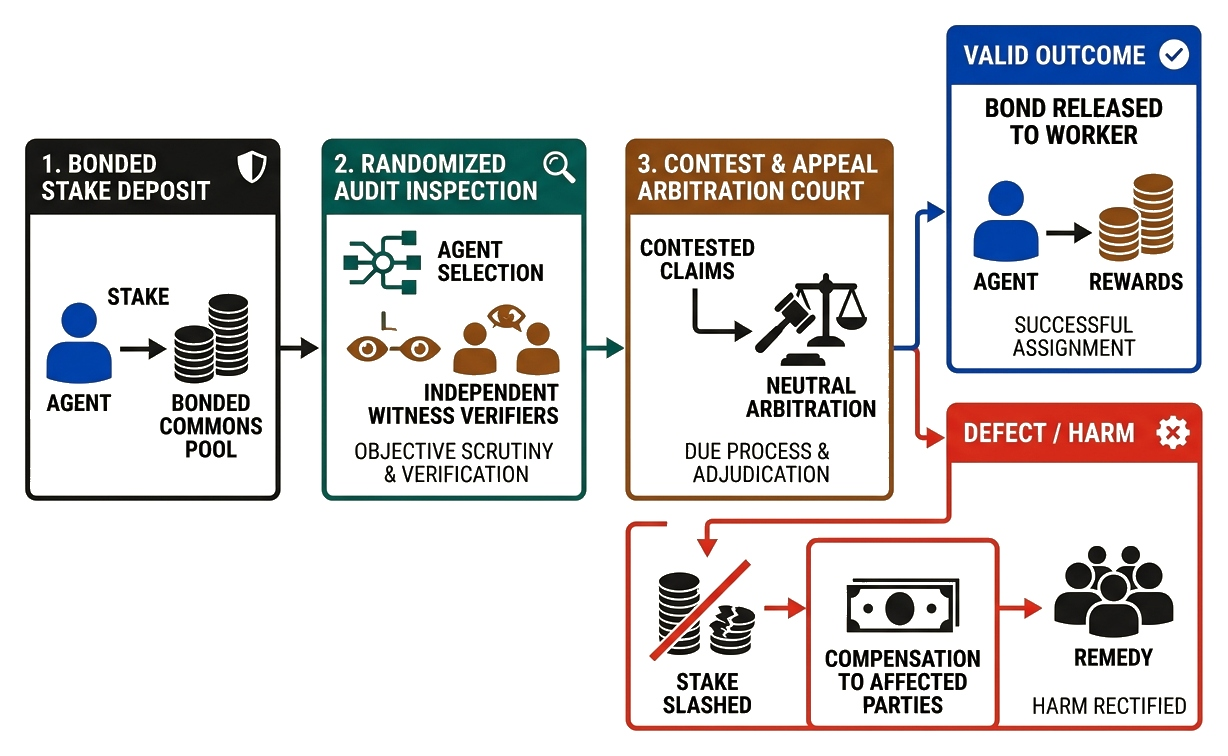
\includegraphics[width=\linewidth,height=8.0cm,keepaspectratio]{figures/fig-spark-prop7-bonded.jpg}
    \end{minipage}
    \tcblower
    \begin{minipage}[t][2.0cm][t]{\linewidth}
      \pdgrotesk\scriptsize
      \textbf{\color{pderror!90!black} Artifact \& Limitation Audit:}\\
      \begin{itemize}[leftmargin=9pt,itemsep=0pt,topsep=0.5pt,parsep=0pt]
        \item Low-resolution clip-art figures with raster scaling artifacts
        \item Broken layout margins with blurry text in arbitration and remedy boxes
        \item Inconsistent line styling between workflow steps and failure branches
      \end{itemize}
    \end{minipage}
  \end{tcolorbox}
\end{minipage}\hfill
\begin{minipage}[t]{0.492\linewidth}
  \begin{tcolorbox}[
    colback=pdcobalt!3,colframe=pdcobalt!85!black,arc=1.5pt,
    boxrule=0.7pt,top=1.5pt,bottom=1.5pt,left=4pt,right=4pt,
    title={\pdgrotesk\footnotesize\bfseries \color{white} B. Authoritative Native Vector Replacement \hfill \texttt{.tex / TikZ / PGF}}
  ]
    \begin{minipage}[c][8.3cm][c]{\linewidth}
      \centering
      \sbox{\pdfigbox}{% fig-spark-prop7-bonded.tex
% Proposition 7: Bonded Execution & Liquidated Damages
% 100% native vector Swiss TikZ spatial replica of fig-spark-prop7-bonded.jpg.

% pd-robot-glyphs.tex
% Authentic vector robot glyphs and system iconography for Port Daddy architectural figures.
% Provides 100% vector replacements matching the AI-generated diagram prototypes.

\ifdefined\pdrobotglyphsloaded\else
\def\pdrobotglyphsloaded{1}

% -----------------------------------------------------------------------------
% 1. Standard Standing Agent Robot (Base Model)
% Args: shift (x,y), color, scale
% -----------------------------------------------------------------------------
\newcommand{\pdrobotbase}[3][1.0]{%
  \begin{scope}[shift={#2},scale=#1]
    % Head
    \draw[fill=#3!85, draw=#3!95!black, line width=0.6pt, rounded corners=2pt] (-0.28, 0.22) rectangle (0.28, 0.58);
    % Dual Antennae
    \draw[line width=0.65pt, draw=#3!95!black] (-0.12, 0.58) -- (-0.16, 0.72);
    \draw[line width=0.65pt, draw=#3!95!black] (0.12, 0.58) -- (0.16, 0.72);
    \fill[pdamber!90!orange] (-0.16, 0.72) circle (0.038);
    \fill[pdamber!90!orange] (0.16, 0.72) circle (0.038);
    % Screen / Visor
    \draw[fill=hhink!90, draw=none, rounded corners=1.2pt] (-0.22, 0.28) rectangle (0.22, 0.52);
    % Eyes
    \fill[pdteal!35!white] (-0.11, 0.40) circle (0.04);
    \fill[pdteal!35!white] (0.11, 0.40) circle (0.04);
    % Mouth bar
    \draw[pdteal!35!white, line width=0.4pt] (-0.07, 0.33) -- (0.07, 0.33);
    % Ear bolts
    \draw[fill=pdslate!60, draw=#3!95!black, line width=0.4pt] (-0.32, 0.35) rectangle (-0.28, 0.45);
    \draw[fill=pdslate!60, draw=#3!95!black, line width=0.4pt] (0.28, 0.35) rectangle (0.32, 0.45);
    % Neck
    \draw[fill=pdslate!70, draw=#3!95!black, line width=0.4pt] (-0.08, 0.16) rectangle (0.08, 0.22);
    % Body / Torso
    \draw[fill=#3!85, draw=#3!95!black, line width=0.6pt, rounded corners=2pt] (-0.32, -0.28) rectangle (0.32, 0.16);
    % Chest panel
    \draw[fill=pdpage, draw=#3!70!black, line width=0.35pt, rounded corners=1pt] (-0.22, -0.12) rectangle (0.22, 0.10);
    \fill[pdhealth] (-0.13, -0.01) circle (0.03);
    \fill[pdamber] (0.0, -0.01) circle (0.03);
    \fill[pderror] (0.13, -0.01) circle (0.03);
    % Arms
    \draw[fill=#3!75, draw=#3!95!black, line width=0.45pt, rounded corners=1.2pt] (-0.44, -0.20) rectangle (-0.32, 0.10);
    \draw[fill=#3!75, draw=#3!95!black, line width=0.45pt, rounded corners=1.2pt] (0.32, -0.20) rectangle (0.44, 0.10);
    % Legs & Feet
    \draw[fill=pdslate!80, draw=#3!95!black, line width=0.45pt] (-0.24, -0.46) rectangle (-0.09, -0.28);
    \draw[fill=pdslate!80, draw=#3!95!black, line width=0.45pt] (0.09, -0.46) rectangle (0.24, -0.28);
    \draw[fill=pdslate!90!black, draw=#3!95!black, line width=0.45pt, rounded corners=1pt] (-0.28, -0.52) rectangle (-0.05, -0.44);
    \draw[fill=pdslate!90!black, draw=#3!95!black, line width=0.45pt, rounded corners=1pt] (0.05, -0.52) rectangle (0.28, -0.44);
  \end{scope}
}

% -----------------------------------------------------------------------------
% 2. Robot Holding Voting / Lease Token Tablet
% -----------------------------------------------------------------------------
\newcommand{\pdrobottoken}[3][1.0]{%
  \begin{scope}[shift={#2},scale=#1]
    % Head
    \draw[fill=#3!85, draw=#3!95!black, line width=0.6pt, rounded corners=2pt] (-0.28, 0.22) rectangle (0.28, 0.58);
    % Antenna
    \draw[line width=0.65pt, draw=#3!95!black] (0, 0.58) -- (0, 0.73);
    \fill[pdamber!90!orange] (0, 0.73) circle (0.04);
    % Screen / Visor
    \draw[fill=hhink!90, draw=none, rounded corners=1.2pt] (-0.22, 0.28) rectangle (0.22, 0.52);
    \fill[pdteal!35!white] (-0.11, 0.40) circle (0.04);
    \fill[pdteal!35!white] (0.11, 0.40) circle (0.04);
    \draw[pdteal!35!white, line width=0.4pt] (-0.07, 0.33) -- (0.07, 0.33);
    % Neck
    \draw[fill=pdslate!70, draw=#3!95!black, line width=0.4pt] (-0.08, 0.16) rectangle (0.08, 0.22);
    % Body
    \draw[fill=#3!85, draw=#3!95!black, line width=0.6pt, rounded corners=2pt] (-0.32, -0.28) rectangle (0.32, 0.16);
    % Legs & Feet
    \draw[fill=pdslate!80, draw=#3!95!black, line width=0.45pt] (-0.24, -0.46) rectangle (-0.09, -0.28);
    \draw[fill=pdslate!80, draw=#3!95!black, line width=0.45pt] (0.09, -0.46) rectangle (0.24, -0.28);
    \draw[fill=pdslate!90!black, draw=#3!95!black, line width=0.45pt, rounded corners=1pt] (-0.28, -0.52) rectangle (-0.05, -0.44);
    \draw[fill=pdslate!90!black, draw=#3!95!black, line width=0.45pt, rounded corners=1pt] (0.05, -0.52) rectangle (0.28, -0.44);
    % Arms holding tablet
    \draw[fill=#3!75, draw=#3!95!black, line width=0.45pt] (-0.42, -0.08) -- (-0.22, 0.05) -- (-0.18, 0.0) -- (-0.35, -0.13) -- cycle;
    \draw[fill=#3!75, draw=#3!95!black, line width=0.45pt] (0.42, -0.08) -- (0.22, 0.05) -- (0.18, 0.0) -- (0.35, -0.13) -- cycle;
    % Tablet
    \draw[fill=pdpage, draw=pdcobalt, line width=0.55pt, rounded corners=1.2pt] (-0.24, -0.18) rectangle (0.24, 0.18);
    \node[font=\fontsize{3.8}{4.5}\selectfont\bfseries\color{pdcobalt}] at (0, 0.06) {VOTING};
    \node[font=\fontsize{3.5}{4.2}\selectfont\bfseries\color{hhink}] at (0, -0.06) {TOKEN};
  \end{scope}
}

% -----------------------------------------------------------------------------
% 3. Robot at Laptop / Deliberation
% -----------------------------------------------------------------------------
\newcommand{\pdrobotlaptop}[3][1.0]{%
  \begin{scope}[shift={#2},scale=#1]
    % Head (Tilted slightly forward)
    \draw[fill=#3!85, draw=#3!95!black, line width=0.6pt, rounded corners=2pt] (-0.26, 0.22) rectangle (0.26, 0.56);
    % Dual Antennae
    \draw[line width=0.65pt, draw=#3!95!black] (-0.10, 0.56) -- (-0.14, 0.70);
    \draw[line width=0.65pt, draw=#3!95!black] (0.10, 0.56) -- (0.14, 0.70);
    \fill[pdteal] (-0.14, 0.70) circle (0.038);
    \fill[pdteal] (0.14, 0.70) circle (0.038);
    % Visor
    \draw[fill=hhink!90, draw=none, rounded corners=1.2pt] (-0.20, 0.28) rectangle (0.20, 0.50);
    \fill[pdteal!40!white] (-0.10, 0.38) circle (0.038);
    \fill[pdteal!40!white] (0.10, 0.38) circle (0.038);
    % Body
    \draw[fill=#3!85, draw=#3!95!black, line width=0.6pt, rounded corners=2pt] (-0.30, -0.26) rectangle (0.30, 0.18);
    % Legs (Seated)
    \draw[fill=pdslate!80, draw=#3!95!black, line width=0.45pt] (-0.25, -0.38) rectangle (0.25, -0.26);
    % Desk surface
    \draw[line width=1.0pt, pdslate!80!black] (-0.6, -0.38) -- (0.7, -0.38);
    % Laptop Base
    \draw[fill=pdslate!40, draw=pdslate!90!black, line width=0.45pt] (-0.05, -0.38) -- (0.50, -0.38) -- (0.46, -0.33) -- (-0.02, -0.33) -- cycle;
    % Laptop Screen
    \draw[fill=pdcobalt!90!black, draw=pdslate!90!black, line width=0.5pt, rounded corners=1pt] (0.42, -0.33) -- (0.52, 0.05) -- (0.15, 0.05) -- (0.08, -0.33) -- cycle;
    % Glowing Screen Text
    \draw[pdteal!50!white, line width=0.4pt] (0.18, -0.03) -- (0.42, -0.03);
    \draw[pdteal!50!white, line width=0.4pt] (0.16, -0.12) -- (0.38, -0.12);
    \draw[pdteal!50!white, line width=0.4pt] (0.14, -0.21) -- (0.34, -0.21);
    % Arms on keyboard
    \draw[fill=#3!75, draw=#3!95!black, line width=0.45pt] (-0.22, 0.05) to[out=-20,in=160] (0.12, -0.30) -- (0.18, -0.33) -- (-0.18, -0.05) -- cycle;
  \end{scope}
}

% -----------------------------------------------------------------------------
% 4. Red-and-White Disablement Barrier
% -----------------------------------------------------------------------------
\newcommand{\pdbarrierline}[4]{% (x1, y1) to (x2, y2)
  \draw[line width=4.5pt, white] (#1,#2) -- (#3,#4);
  \draw[line width=4.5pt, pderror, dashed, dash pattern=on 6pt off 6pt] (#1,#2) -- (#3,#4);
  \draw[line width=0.6pt, pderror!80!black] (#1,#2) -- (#3,#4);
}

% -----------------------------------------------------------------------------
% 5. Vector Iconography Definitions
% -----------------------------------------------------------------------------
% Crossed Tools (Wrench + Screwdriver)
\newcommand{\pdicontools}[2][1.0]{%
  \begin{scope}[shift={#2},scale=#1]
    \draw[line width=1.4pt, pdslate!80!black, line cap=round] (-0.25,-0.25) -- (0.25,0.25);
    \draw[line width=1.4pt, pdrust!90!black, line cap=round] (-0.25,0.25) -- (0.25,-0.25);
    \draw[fill=pdslate!90!black, line width=0.4pt] (0.18,0.18) circle (0.10);
    \fill[white] (0.20,0.20) circle (0.04);
    \draw[fill=pdrust!90!black, line width=0.4pt] (0.20,-0.22) rectangle (0.26,-0.16);
  \end{scope}
}

% Git Branch
\newcommand{\pdicongit}[2][1.0]{%
  \begin{scope}[shift={#2},scale=#1]
    \draw[line width=1.1pt, pdteal!90!black] (0,-0.32) -- (0,0.32);
    \draw[line width=1.1pt, pdteal!90!black] (0,-0.08) to[out=45,in=180] (0.24,0.16);
    \fill[pdteal!90!black] (0,-0.24) circle (0.06);
    \fill[pdteal!90!black] (0,0.24) circle (0.06);
    \fill[pdteal!90!black] (0.24,0.16) circle (0.06);
  \end{scope}
}

% Network Globe
\newcommand{\pdiconglobe}[2][1.0]{%
  \begin{scope}[shift={#2},scale=#1]
    \draw[line width=0.7pt, pdcobalt!85!black] (0,0) circle (0.28);
    \draw[line width=0.5pt, pdcobalt!70] (0,0) ellipse (0.13 and 0.28);
    \draw[line width=0.5pt, pdcobalt!70] (-0.28,0) -- (0.28,0);
    \draw[line width=0.5pt, pdcobalt!70] (-0.24,0.14) -- (0.24,0.14);
    \draw[line width=0.5pt, pdcobalt!70] (-0.24,-0.14) -- (0.24,-0.14);
  \end{scope}
}

% Host OS Gear / Process
\newcommand{\pdicongear}[2][1.0]{%
  \begin{scope}[shift={#2},scale=#1]
    \fill[pdslate!75!black] (0,0) circle (0.22);
    \foreach \a in {0,45,90,135,180,225,270,315} {
      \fill[pdslate!75!black] (\a:0.26) circle (0.055);
    }
    \fill[white] (0,0) circle (0.09);
  \end{scope}
}

% Stopwatch / Timer
\newcommand{\pdicontimer}[2][1.0]{%
  \begin{scope}[shift={#2},scale=#1]
    \draw[line width=0.75pt, pdamber!90!black] (0,0) circle (0.25);
    \draw[line width=0.8pt, pdamber!90!black] (0,0.25) -- (0,0.33);
    \draw[line width=1.0pt, pdamber!90!black] (-0.06,0.33) -- (0.06,0.33);
    \draw[line width=0.75pt, pdamber!90!black] (0,0) -- (0,0.14);
    \draw[line width=0.75pt, pdamber!90!black] (0,0) -- (0.11,0.05);
    \fill[pdamber!90!black] (0,0) circle (0.035);
  \end{scope}
}

% Hardware Crash / Lightning Burst
\newcommand{\pdiconcrash}[2][1.0]{%
  \begin{scope}[shift={#2},scale=#1]
    \fill[pderror!90!black] (0.06,0.32) -- (-0.12,0.04) -- (-0.02,0.04) -- (-0.14,-0.32) -- (0.12,-0.02) -- (0.02,-0.02) -- cycle;
  \end{scope}
}

% Shield with Checkmark
\newcommand{\pdiconshieldcheck}[2][1.0]{%
  \begin{scope}[shift={#2},scale=#1]
    \fill[pdcobalt!90!black] (0,0.32) -- (0.26,0.20) to[out=-70,in=45] (0,-0.32) to[out=135,in=-110] (-0.26,0.20) -- cycle;
    \draw[line width=1.1pt, white, line cap=round, line join=round] (-0.11,-0.02) -- (-0.03,-0.12) -- (0.13,0.10);
  \end{scope}
}

% Padlock
\newcommand{\pdiconlock}[2][1.0]{%
  \begin{scope}[shift={#2},scale=#1]
    % Shackle
    \draw[line width=0.9pt, pdslate!80!black] (-0.12,0.05) -- (-0.12,0.18) arc (180:0:0.12) -- (0.12,0.05);
    % Body
    \draw[fill=pderror!85!black, draw=pderror!95!black, line width=0.5pt, rounded corners=1pt] (-0.18,-0.20) rectangle (0.18,0.06);
    % Keyhole
    \fill[white] (0,-0.04) circle (0.035);
    \draw[line width=0.6pt, white] (0,-0.04) -- (0,-0.13);
  \end{scope}
}

% Speedometer / Spend Cap
\newcommand{\pdiconspeedometer}[2][1.0]{%
  \begin{scope}[shift={#2},scale=#1]
    \draw[line width=1.0pt, pdteal!90!black] (-0.28,-0.04) arc (180:40:0.28);
    \draw[line width=1.0pt, pderror] (40:0.28) arc (40:0:0.28);
    \draw[line width=0.8pt, hhink, line cap=round] (0,-0.04) -- (0.12,0.14);
    \fill[hhink] (0,-0.04) circle (0.05);
  \end{scope}
}

% Sparkle Broom / Hygiene Wand
\newcommand{\pdiconbroom}[2][1.0]{%
  \begin{scope}[shift={#2},scale=#1]
    \draw[line width=1.2pt, pdteal!90!black, line cap=round] (-0.2,-0.2) -- (0.15,0.15);
    % Sparkles
    \fill[pdamber!90!orange] (0.22,0.22) circle (0.04);
    \fill[pdteal] (0.05,0.26) circle (0.03);
    \fill[pdteal] (0.26,0.05) circle (0.03);
  \end{scope}
}

% Host Terminal Substrate
\newcommand{\pdiconterminal}[2][1.0]{%
  \begin{scope}[shift={#2},scale=#1]
    \draw[fill=hhink!95, draw=pdslate!80, line width=0.6pt, rounded corners=1.5pt] (-0.35,-0.25) rectangle (0.35,0.25);
    \draw[fill=pderror] (-0.26,0.18) circle (0.025);
    \fill[pdamber] (-0.18,0.18) circle (0.025);
    \fill[pdhealth] (-0.10,0.18) circle (0.025);
    \node[font=\fontsize{4.5}{5}\selectfont\ttfamily\color{pdhealth}] at (0,-0.05) {>\_};
  \end{scope}
}

% Coins Stack
\newcommand{\pdiconcoins}[2][1.0]{%
  \begin{scope}[shift={#2},scale=#1]
    \foreach \y in {-0.24, -0.12, 0.0, 0.12} {
      \draw[fill=pdamber!80!orange, draw=pdamber!95!black, line width=0.45pt] (0,\y) ellipse (0.24 and 0.07);
    }
  \end{scope}
}

% Tall Coins Stack
\newcommand{\pdiconcoinstall}[2][1.0]{%
  \begin{scope}[shift={#2},scale=#1]
    \foreach \y in {-0.30, -0.18, -0.06, 0.06, 0.18, 0.30} {
      \draw[fill=pdamber!80!orange, draw=pdamber!95!black, line width=0.45pt] (0,\y) ellipse (0.24 and 0.07);
    }
  \end{scope}
}

% Slashed Coins (Stake Slashed)
\newcommand{\pdiconcoinslashed}[2][1.0]{%
  \begin{scope}[shift={#2},scale=#1]
    \foreach \y in {-0.20, -0.08, 0.04, 0.16} {
      \draw[fill=pdamber!70!white, draw=pdamber!80!black, line width=0.45pt] (0,\y) ellipse (0.22 and 0.065);
    }
    \draw[line width=1.5pt, pderror, line cap=round] (-0.26,-0.24) -- (0.26,0.24);
  \end{scope}
}

% Magnifying Glass (Audit Inspection)
\newcommand{\pdiconmagnifier}[2][1.0]{%
  \begin{scope}[shift={#2},scale=#1]
    \draw[line width=0.9pt, pdteal!90!black] (0,0.06) circle (0.16);
    \draw[line width=1.4pt, pdteal!90!black, line cap=round] (0.12,-0.06) -- (0.26,-0.20);
    \fill[white] (-0.04,0.10) circle (0.04);
  \end{scope}
}

% Arbitration Gavel & Scales of Justice
\newcommand{\pdiconarbitration}[2][1.0]{%
  \begin{scope}[shift={#2},scale=#1]
    % Central post
    \draw[line width=0.8pt, pdrust!90!black] (0.15,-0.20) -- (0.15,0.22);
    \draw[line width=0.8pt, pdrust!90!black] (-0.05,0.18) -- (0.35,0.18);
    \draw[line width=0.5pt, pdrust!80] (-0.05,0.18) -- (-0.12,0.02) -- (0.02,0.02) -- cycle;
    \draw[line width=0.5pt, pdrust!80] (0.35,0.18) -- (0.28,0.02) -- (0.42,0.02) -- cycle;
    % Gavel
    \draw[line width=1.4pt, pdrust!95!black, line cap=round] (-0.30,-0.18) -- (-0.10,0.05);
    \draw[fill=pdrust!90!black, draw=pdrust!95!black, line width=0.5pt, rounded corners=1pt] (-0.22,0.0) -- (-0.12,0.12) -- (-0.02,0.04) -- (-0.12,-0.08) -- cycle;
  \end{scope}
}

% Cash Bill / Liquidated Damages
\newcommand{\pdiconcash}[2][1.0]{%
  \begin{scope}[shift={#2},scale=#1]
    \draw[fill=white, draw=pdslate!90!black, line width=0.6pt, rounded corners=1.5pt] (-0.35,-0.20) rectangle (0.35,0.20);
    \draw[line width=0.5pt, pdteal!80!black] (-0.28,-0.14) rectangle (0.28,0.14);
    \fill[pdteal!90!black] (0,0) circle (0.08);
    \fill[pdteal!90!black] (-0.22,0) circle (0.035);
    \fill[pdteal!90!black] (0.22,0) circle (0.035);
  \end{scope}
}

% Group of People / Remedy
\newcommand{\pdicongrouppeople}[2][1.0]{%
  \begin{scope}[shift={#2},scale=#1]
    % Center person
    \fill[hhink] (0,0.12) circle (0.09);
    \fill[hhink] (-0.15,-0.20) to[out=70,in=180] (0,-0.02) to[out=0,in=110] (0.15,-0.20) -- cycle;
    % Left person
    \fill[hhgray!90!black] (-0.22,0.06) circle (0.075);
    \fill[hhgray!90!black] (-0.34,-0.20) to[out=70,in=180] (-0.22,-0.06) to[out=0,in=110] (-0.10,-0.20) -- cycle;
    % Right person
    \fill[hhgray!90!black] (0.22,0.06) circle (0.075);
    \fill[hhgray!90!black] (0.10,-0.20) to[out=70,in=180] (0.22,-0.06) to[out=0,in=110] (0.34,-0.20) -- cycle;
  \end{scope}
}

% Database Cylinder
\newcommand{\pdicondatabase}[2][1.0]{%
  \begin{scope}[shift={#2},scale=#1]
    \draw[fill=pdslate!20, draw=pdslate!90!black, line width=0.6pt] (-0.25,-0.15) rectangle (0.25,0.15);
    \draw[fill=pdslate!30, draw=pdslate!90!black, line width=0.5pt] (0,0.15) ellipse (0.25 and 0.08);
    \draw[draw=pdslate!90!black, line width=0.5pt] (-0.25,0) arc (180:360:0.25 and 0.08);
    \draw[draw=pdslate!90!black, line width=0.5pt] (-0.25,-0.15) arc (180:360:0.25 and 0.08);
  \end{scope}
}

% Signed Document / Witness Receipts
\newcommand{\pdicondocument}[2][1.0]{%
  \begin{scope}[shift={#2},scale=#1]
    \draw[fill=white, draw=pdslate!90!black, line width=0.55pt] (-0.18,-0.24) -- (0.10,-0.24) -- (0.18,-0.16) -- (0.18,0.24) -- (-0.18,0.24) -- cycle;
    \draw[draw=pdslate!80, line width=0.45pt] (0.10,-0.24) -- (0.10,-0.16) -- (0.18,-0.16);
    \draw[pdslate!70, line width=0.4pt] (-0.12,0.16) -- (0.12,0.16);
    \draw[pdslate!70, line width=0.4pt] (-0.12,0.08) -- (0.12,0.08);
    \draw[pdslate!70, line width=0.4pt] (-0.12,0.00) -- (0.06,0.00);
    % Feather / quill
    \draw[line width=0.7pt, pdcobalt!80!black] (0.08,-0.12) to[out=45,in=-45] (0.24,0.06);
  \end{scope}
}

% Merkle Inclusion Proof Tree
\newcommand{\pdiconmerkle}[2][1.0]{%
  \begin{scope}[shift={#2},scale=#1]
    % Root
    \draw[line width=0.5pt, pdslate!80] (0,0.20) -- (-0.16,0.04);
    \draw[line width=0.5pt, pdslate!80] (0,0.20) -- (0.16,0.04);
    \draw[line width=0.5pt, pdslate!80] (-0.16,0.04) -- (-0.24,-0.14);
    \draw[line width=0.5pt, pdslate!80] (-0.16,0.04) -- (-0.08,-0.14);
    \draw[line width=0.5pt, pdslate!80] (0.16,0.04) -- (0.08,-0.14);
    \draw[line width=0.5pt, pdslate!80] (0.16,0.04) -- (0.24,-0.14);
    \draw[fill=white, draw=pdslate!90!black, line width=0.4pt] (-0.05,0.16) rectangle (0.05,0.24);
    \draw[fill=white, draw=pdslate!90!black, line width=0.4pt] (-0.20,0.0) rectangle (-0.12,0.08);
    \draw[fill=white, draw=pdslate!90!black, line width=0.4pt] (0.12,0.0) rectangle (0.20,0.08);
    \draw[fill=pdteal!80!white, draw=pdteal!95!black, line width=0.5pt] (-0.28,-0.18) rectangle (-0.20,-0.10);
    \draw[fill=white, draw=pdslate!90!black, line width=0.4pt] (-0.12,-0.18) rectangle (-0.04,-0.10);
    \draw[fill=white, draw=pdslate!90!black, line width=0.4pt] (0.04,-0.18) rectangle (0.12,-0.10);
    \draw[fill=white, draw=pdslate!90!black, line width=0.4pt] (0.20,-0.18) rectangle (0.28,-0.10);
  \end{scope}
}

% Key (Cryptographic Key / Capability Key)
\newcommand{\pdiconkey}[2][1.0]{%
  \begin{scope}[shift={#2},scale=#1]
    \draw[line width=0.8pt, pdamber!95!black] (0, 0.12) circle (0.14);
    \fill[white] (0, 0.12) circle (0.06);
    \draw[line width=0.85pt, pdamber!95!black] (0, -0.02) -- (0, -0.26);
    \draw[line width=0.7pt, pdamber!95!black] (0, -0.14) -- (0.10, -0.14);
    \draw[line width=0.7pt, pdamber!95!black] (0, -0.22) -- (0.08, -0.22);
  \end{scope}
}

\def\pdiconclock{\pdicontimer}
\def\pdiconlightning{\pdiconcrash}

\fi

\pdfigurehue{pdcobalt}%
\begin{tikzpicture}[pd figure,x=1cm,y=1cm]
  \tikzset{
    stagecard/.style={draw=pdslate!80!black,line width=0.7pt,fill=white,rounded corners=2.5pt},
    stageheader/.style={font=\fontsize{5.2}{6.2}\selectfont\bfseries\color{white},inner sep=3pt,rounded corners=2pt},
    sublabel/.style={font=\fontsize{4.6}{5.6}\selectfont\bfseries\color{hhink},align=center},
    tinylabel/.style={font=\fontsize{4.0}{4.8}\selectfont\color{hhgray!90!black},align=center}
  }

  % =========================================================================
  % CARD 1: 1. BONDED STAKE DEPOSIT (x in [0.1, 2.9], y in [1.5, 5.1])
  % =========================================================================
  \draw[stagecard] (0.1, 1.5) rectangle (2.9, 5.1);
  % Header
  \draw[fill=hhink!95,draw=none,rounded corners=2pt] (0.1, 4.65) rectangle (2.9, 5.1);
  \node[anchor=west,font=\fontsize{4.4}{5.4}\selectfont\bfseries\color{white}] at (0.18, 4.87) {1. BONDED STAKE DEPOSIT};
  \pdiconshieldcheck[0.45]{(2.7, 4.87)}

  % Agent Robot
  \pdrobotbase[0.55]{(0.7, 3.25)}{pdcobalt}
  \node[sublabel] at (0.7, 2.45) {AGENT};

  % Arrow: Stake
  \draw[pd arrow,line width=0.8pt,hhink] (1.15, 3.25) -- (1.65, 3.25);
  \node[sublabel] at (1.4, 3.5) {STAKE};

  % Bonded Commons Pool (Coins Stack)
  \pdiconcoinstall[0.85]{(2.15, 3.25)}
  \node[sublabel] at (2.15, 2.40) {BONDED\\COMMONS\\POOL};

  % Arrow Card 1 -> Card 2
  \draw[pd arrow,line width=1.0pt,hhink] (2.9, 3.3) -- (3.35, 3.3);

  % =========================================================================
  % CARD 2: 2. RANDOMIZED AUDIT INSPECTION (x in [3.35, 6.35], y in [1.5, 5.1])
  % =========================================================================
  \draw[stagecard,draw=pdteal!85!black] (3.35, 1.5) rectangle (6.35, 5.1);
  % Header
  \draw[fill=pdteal!85!black,draw=none,rounded corners=2pt] (3.35, 4.65) rectangle (6.35, 5.1);
  \node[anchor=west,font=\fontsize{4.8}{5.8}\selectfont\bfseries\color{white}] at (3.45, 4.87) {2. RANDOMIZED AUDIT};
  \pdiconmagnifier[0.5]{(6.1, 4.87)}

  % Agent Selection Block
  \draw[line width=0.8pt,pdteal!85!black] (3.6, 4.1) -- (3.9, 4.1);
  \draw[line width=0.8pt,pdteal!85!black] (3.9, 4.3) -- (3.9, 3.9);
  \draw[line width=0.6pt,pdteal!85!black] (3.9, 4.3) -- (4.15, 4.3);
  \draw[line width=0.6pt,pdteal!85!black] (3.9, 4.1) -- (4.15, 4.1);
  \draw[line width=0.6pt,pdteal!85!black] (3.9, 3.9) -- (4.15, 3.9);
  \draw[fill=pdteal!20,draw=pdteal!85!black,line width=0.4pt] (4.15, 4.23) rectangle (4.32, 4.37);
  \draw[fill=pdteal!20,draw=pdteal!85!black,line width=0.4pt] (4.15, 4.03) rectangle (4.32, 4.17);
  \draw[fill=pdteal!20,draw=pdteal!85!black,line width=0.4pt] (4.15, 3.83) rectangle (4.32, 3.97);
  \node[anchor=west,sublabel] at (4.45, 4.1) {AGENT\\SELECTION};

  % Independent Witness Verifiers
  \pdrobotbase[0.45]{(4.35, 3.05)}{pdteal}
  \pdrobotbase[0.45]{(5.35, 3.05)}{pdrust}
  \draw[fill=white,draw=pdteal!80!black,line width=0.4pt] (4.0, 3.2) circle (0.12);
  \fill[pdteal!80!black] (4.0, 3.2) circle (0.05);
  \draw[fill=white,draw=pdteal!80!black,line width=0.4pt] (4.25, 3.2) circle (0.12);
  \fill[pdteal!80!black] (4.25, 3.2) circle (0.05);
  \node[sublabel] at (4.85, 2.45) {INDEPENDENT\\WITNESS VERIFIERS};
  \node[tinylabel] at (4.85, 1.95) {OBJECTIVE SCRUTINY\\AND VERIFICATION};

  % Arrow Card 2 -> Card 3
  \draw[pd arrow,line width=1.0pt,pdteal!85!black] (6.35, 3.3) -- (6.8, 3.3);

  % =========================================================================
  % CARD 3: 3. CONTEST & APPEAL ARBITRATION (x in [6.8, 9.8], y in [1.5, 5.1])
  % =========================================================================
  \draw[stagecard,draw=pdrust!85!black] (6.8, 1.5) rectangle (9.8, 5.1);
  % Header
  \draw[fill=pdrust!90!black,draw=none,rounded corners=2pt] (6.8, 4.65) rectangle (9.8, 5.1);
  \node[anchor=west,font=\fontsize{4.8}{5.8}\selectfont\bfseries\color{white}] at (6.9, 4.87) {3. CONTEST \& APPEAL COURT};

  % Contested Claims & Arbitration
  \node[sublabel] at (7.5, 4.25) {CONTESTED\\CLAIMS};
  \draw[pd arrow,line width=0.7pt,hhink] (7.5, 3.9) |- (8.1, 3.4);
  \pdiconarbitration[0.9]{(8.85, 3.45)}
  \node[sublabel] at (8.3, 2.65) {NEUTRAL\\ARBITRATION};
  \node[tinylabel] at (8.3, 1.95) {DUE PROCESS \&\\ADJUDICATION};

  % Forking arrows from Card 3 to Outcomes
  \draw[pd arrow,line width=1.0pt,pdcobalt] (9.8, 3.8) -- (10.25, 3.8) |- (10.4, 4.1);
  \draw[pd arrow,line width=1.0pt,pderror] (9.8, 2.6) -- (10.25, 2.6) |- (10.4, 2.1);

  % =========================================================================
  % OUTCOME 1: VALID OUTCOME (Top Right, x in [10.4, 13.5], y in [2.9, 5.1])
  % =========================================================================
  \draw[stagecard,draw=pdcobalt!85!black] (10.4, 2.85) rectangle (13.5, 5.1);
  \draw[fill=pdcobalt!90!black,draw=none,rounded corners=2pt] (10.4, 4.65) rectangle (13.5, 5.1);
  \node[anchor=west,font=\fontsize{5.2}{6.2}\selectfont\bfseries\color{white}] at (10.55, 4.87) {VALID OUTCOME};
  \pdiconshieldcheck[0.45]{(13.25, 4.87)}

  \node[font=\fontsize{4.8}{5.8}\selectfont\bfseries\color{pdcobalt!90!black},align=center] at (11.95, 4.35) {BOND RELEASED TO WORKER};
  \pdrobotbase[0.45]{(10.95, 3.55)}{pdcobalt}
  \node[sublabel] at (10.95, 3.1) {AGENT};

  \draw[pd arrow,line width=0.8pt,hhink] (11.45, 3.55) -- (11.95, 3.55);

  \pdiconcoinstall[0.75]{(12.5, 3.55)}
  \node[sublabel] at (12.5, 3.1) {REWARDS};

  % =========================================================================
  % OUTCOME 2: DEFECT / HARM (x in [10.4, 13.5], y in [1.5, 2.65])
  % =========================================================================
  \draw[stagecard,draw=pderror!90!black] (10.4, 1.5) rectangle (13.5, 2.65);
  \draw[fill=pderror!90!black,draw=none,rounded corners=2pt] (10.4, 2.25) rectangle (13.5, 2.65);
  \node[anchor=west,font=\fontsize{5.0}{6.0}\selectfont\bfseries\color{white}] at (10.55, 2.45) {DEFECT / HARM};
  \pdiconcrash[0.45]{(13.25, 2.45)}

  \node[sublabel,pderror!90!black] at (11.95, 1.85) {BREACH DETECTED};

  % Slashed Stake & Remedy workflow below (y in [0.05, 1.35])
  \draw[stagecard,draw=pderror!70!black,dashed,fill=pdpage!30] (3.35, 0.05) rectangle (13.5, 1.35);

  % Connector from Defect card down into remediation tray
  \draw[line width=0.8pt,pderror,pd arrow] (10.4, 1.7) -| (3.15, 0.7) -- (3.35, 0.7);

  % Step A: Stake Slashed
  \pdiconcoinslashed[0.7]{(4.45, 0.75)}
  \node[sublabel,color=pderror!90!black] at (4.45, 0.25) {STAKE SLASHED};

  \draw[pd arrow,line width=0.8pt,pderror] (5.45, 0.75) -- (6.05, 0.75);

  % Step B: Compensation
  \pdiconcash[0.8]{(7.45, 0.75)}
  \node[sublabel] at (7.45, 0.25) {COMPENSATION TO PARTIES};

  \draw[pd arrow,line width=0.8pt,pderror] (8.9, 0.75) -- (9.5, 0.75);

  % Step C: Remedy
  \pdicongrouppeople[0.75]{(11.2, 0.75)}
  \node[sublabel,color=pdteal!90!black] at (11.2, 0.25) {REMEDY: HARM RECTIFIED};

\end{tikzpicture}
}
      \pdautoscale{8.0cm}{\linewidth}
    \end{minipage}
    \tcblower
    \begin{minipage}[t][2.0cm][t]{\linewidth}
      \pdgrotesk\scriptsize
      \textbf{{\color{pdcobalt} Engineering \& Typography Guarantees:}}\\
      \begin{itemize}[leftmargin=9pt,itemsep=0pt,topsep=0.5pt,parsep=0pt]
        \item 3-stage pipeline: Bonded Stake Deposit, Randomized Audit, and Contest Arbitration
        \item Dual-outcome branching: Valid Outcome (Bond Released) vs. Defect/Harm (Stake Slashed)
        \item Integrated remedy sequence: Automatic liquidation and compensation to affected parties
      \end{itemize}
    \end{minipage}
  \end{tcolorbox}
\end{minipage}

\vspace*{0.05cm}
\noindent
\begin{tcolorbox}[
  colback=hhpaper,colframe=hhgray!35,arc=1.5pt,boxrule=0.4pt,
  top=1.5pt,bottom=1.5pt,left=6pt,right=6pt
]
  \pdgrotesk\scriptsize
  \noindent
  \textbf{Visual Substrate:} Lossy Bitmap Raster $\rightarrow$ \textbf{\color{pdcobalt}Native PDF / PostScript Vector}\hfill
  \textbf{Text Engine:} Pixelated Approximations $\rightarrow$ \textbf{\color{pdcobalt}Book Typography (OpenType)}\hfill
  \textbf{Resolution:} Fixed DPI Limit $\rightarrow$ \textbf{\color{pdcobalt}Infinite Resolution ($\infty$)}\hfill
  \textbf{Status:} \textbf{\color{pdteal}RECONCILED \& VERIFIED}
\end{tcolorbox}
\clearpage

% =========================================================================
% PAGE 8: Figure 0.8
% =========================================================================
\noindent
\begin{minipage}[t]{\linewidth}
  \noindent{\pdgrotesk\large\bfseries Figure 0.8 \textperiodcentered\ Proposition 8 Mechanics: Cross-Harbor Relay \& Zero-Trust Federation}\hfill
  {\pdgrotesk\footnotesize\color{hhgray} Section 0.2.8 · Distributed Architecture · Relay Fabric \& Proof Gossip}\\
  \vspace*{0.03cm}
  \noindent{\color{hhgray!40}\rule{\linewidth}{0.5pt}}
\end{minipage}

\vspace*{0.05cm}
\noindent
\begin{minipage}[t]{0.492\linewidth}
  \begin{tcolorbox}[
    colback=pdslate!4,colframe=pdslate!70!black,arc=1.5pt,
    boxrule=0.6pt,top=1.5pt,bottom=1.5pt,left=4pt,right=4pt,
    title={\pdgrotesk\footnotesize\bfseries \color{white} A. AI-Generated Raster Prototype (Diffusion / Nano Banana) \hfill \texttt{.jpg / .png}}
  ]
    \begin{minipage}[c][8.3cm][c]{\linewidth}
      \centering
      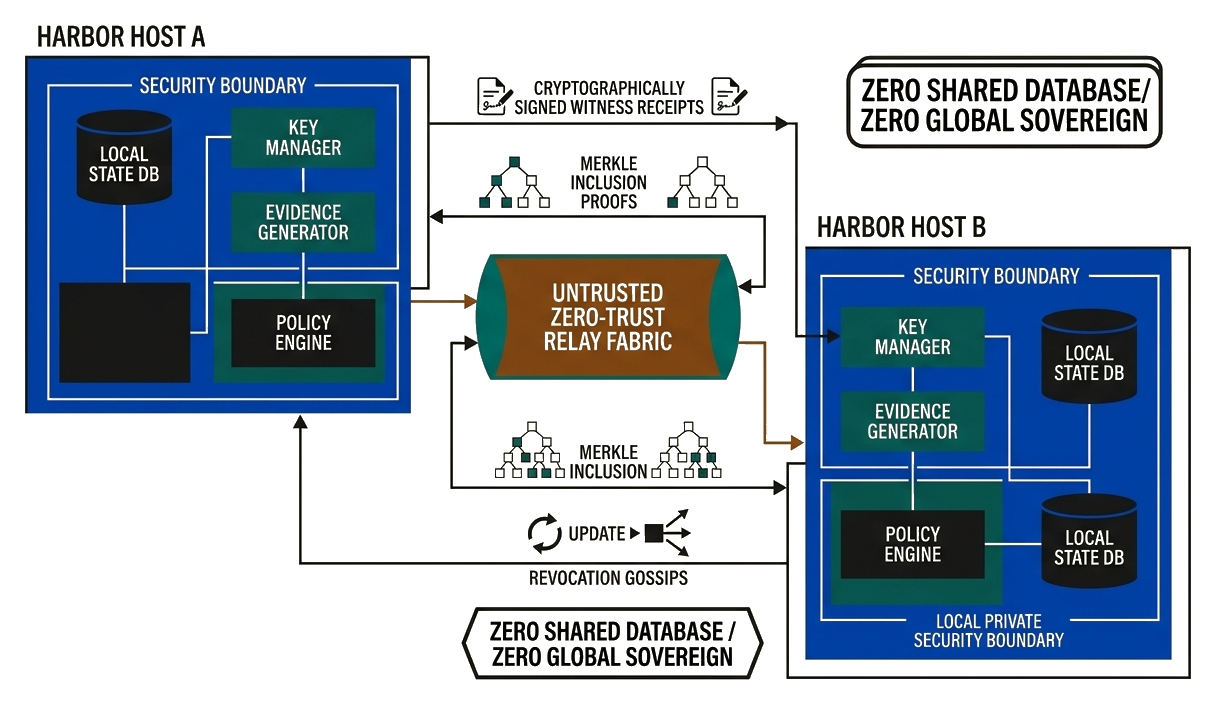
\includegraphics[width=\linewidth,height=8.0cm,keepaspectratio]{figures/fig-spark-prop8-federation.jpg}
    \end{minipage}
    \tcblower
    \begin{minipage}[t][2.0cm][t]{\linewidth}
      \pdgrotesk\scriptsize
      \textbf{\color{pderror!90!black} Artifact \& Limitation Audit:}\\
      \begin{itemize}[leftmargin=9pt,itemsep=0pt,topsep=0.5pt,parsep=0pt]
        \item Heavy raster compression artifacts on database cylinders and security boundaries
        \item Illegible Merkle tree leaf labels and blurry cryptographic signature badges
        \item Disconnected arrows and fuzzy zero-trust relay cylinder boundary
      \end{itemize}
    \end{minipage}
  \end{tcolorbox}
\end{minipage}\hfill
\begin{minipage}[t]{0.492\linewidth}
  \begin{tcolorbox}[
    colback=pdcobalt!3,colframe=pdcobalt!85!black,arc=1.5pt,
    boxrule=0.7pt,top=1.5pt,bottom=1.5pt,left=4pt,right=4pt,
    title={\pdgrotesk\footnotesize\bfseries \color{white} B. Authoritative Native Vector Replacement \hfill \texttt{.tex / TikZ / PGF}}
  ]
    \begin{minipage}[c][8.3cm][c]{\linewidth}
      \centering
      \sbox{\pdfigbox}{% fig-spark-prop8-federation.tex
% Proposition 8: Cross-Harbor Relay & Zero-Trust Federation
% 100% native vector Swiss TikZ spatial replica of fig-spark-prop8-federation.jpg.

% pd-robot-glyphs.tex
% Authentic vector robot glyphs and system iconography for Port Daddy architectural figures.
% Provides 100% vector replacements matching the AI-generated diagram prototypes.

\ifdefined\pdrobotglyphsloaded\else
\def\pdrobotglyphsloaded{1}

% -----------------------------------------------------------------------------
% 1. Standard Standing Agent Robot (Base Model)
% Args: shift (x,y), color, scale
% -----------------------------------------------------------------------------
\newcommand{\pdrobotbase}[3][1.0]{%
  \begin{scope}[shift={#2},scale=#1]
    % Head
    \draw[fill=#3!85, draw=#3!95!black, line width=0.6pt, rounded corners=2pt] (-0.28, 0.22) rectangle (0.28, 0.58);
    % Dual Antennae
    \draw[line width=0.65pt, draw=#3!95!black] (-0.12, 0.58) -- (-0.16, 0.72);
    \draw[line width=0.65pt, draw=#3!95!black] (0.12, 0.58) -- (0.16, 0.72);
    \fill[pdamber!90!orange] (-0.16, 0.72) circle (0.038);
    \fill[pdamber!90!orange] (0.16, 0.72) circle (0.038);
    % Screen / Visor
    \draw[fill=hhink!90, draw=none, rounded corners=1.2pt] (-0.22, 0.28) rectangle (0.22, 0.52);
    % Eyes
    \fill[pdteal!35!white] (-0.11, 0.40) circle (0.04);
    \fill[pdteal!35!white] (0.11, 0.40) circle (0.04);
    % Mouth bar
    \draw[pdteal!35!white, line width=0.4pt] (-0.07, 0.33) -- (0.07, 0.33);
    % Ear bolts
    \draw[fill=pdslate!60, draw=#3!95!black, line width=0.4pt] (-0.32, 0.35) rectangle (-0.28, 0.45);
    \draw[fill=pdslate!60, draw=#3!95!black, line width=0.4pt] (0.28, 0.35) rectangle (0.32, 0.45);
    % Neck
    \draw[fill=pdslate!70, draw=#3!95!black, line width=0.4pt] (-0.08, 0.16) rectangle (0.08, 0.22);
    % Body / Torso
    \draw[fill=#3!85, draw=#3!95!black, line width=0.6pt, rounded corners=2pt] (-0.32, -0.28) rectangle (0.32, 0.16);
    % Chest panel
    \draw[fill=pdpage, draw=#3!70!black, line width=0.35pt, rounded corners=1pt] (-0.22, -0.12) rectangle (0.22, 0.10);
    \fill[pdhealth] (-0.13, -0.01) circle (0.03);
    \fill[pdamber] (0.0, -0.01) circle (0.03);
    \fill[pderror] (0.13, -0.01) circle (0.03);
    % Arms
    \draw[fill=#3!75, draw=#3!95!black, line width=0.45pt, rounded corners=1.2pt] (-0.44, -0.20) rectangle (-0.32, 0.10);
    \draw[fill=#3!75, draw=#3!95!black, line width=0.45pt, rounded corners=1.2pt] (0.32, -0.20) rectangle (0.44, 0.10);
    % Legs & Feet
    \draw[fill=pdslate!80, draw=#3!95!black, line width=0.45pt] (-0.24, -0.46) rectangle (-0.09, -0.28);
    \draw[fill=pdslate!80, draw=#3!95!black, line width=0.45pt] (0.09, -0.46) rectangle (0.24, -0.28);
    \draw[fill=pdslate!90!black, draw=#3!95!black, line width=0.45pt, rounded corners=1pt] (-0.28, -0.52) rectangle (-0.05, -0.44);
    \draw[fill=pdslate!90!black, draw=#3!95!black, line width=0.45pt, rounded corners=1pt] (0.05, -0.52) rectangle (0.28, -0.44);
  \end{scope}
}

% -----------------------------------------------------------------------------
% 2. Robot Holding Voting / Lease Token Tablet
% -----------------------------------------------------------------------------
\newcommand{\pdrobottoken}[3][1.0]{%
  \begin{scope}[shift={#2},scale=#1]
    % Head
    \draw[fill=#3!85, draw=#3!95!black, line width=0.6pt, rounded corners=2pt] (-0.28, 0.22) rectangle (0.28, 0.58);
    % Antenna
    \draw[line width=0.65pt, draw=#3!95!black] (0, 0.58) -- (0, 0.73);
    \fill[pdamber!90!orange] (0, 0.73) circle (0.04);
    % Screen / Visor
    \draw[fill=hhink!90, draw=none, rounded corners=1.2pt] (-0.22, 0.28) rectangle (0.22, 0.52);
    \fill[pdteal!35!white] (-0.11, 0.40) circle (0.04);
    \fill[pdteal!35!white] (0.11, 0.40) circle (0.04);
    \draw[pdteal!35!white, line width=0.4pt] (-0.07, 0.33) -- (0.07, 0.33);
    % Neck
    \draw[fill=pdslate!70, draw=#3!95!black, line width=0.4pt] (-0.08, 0.16) rectangle (0.08, 0.22);
    % Body
    \draw[fill=#3!85, draw=#3!95!black, line width=0.6pt, rounded corners=2pt] (-0.32, -0.28) rectangle (0.32, 0.16);
    % Legs & Feet
    \draw[fill=pdslate!80, draw=#3!95!black, line width=0.45pt] (-0.24, -0.46) rectangle (-0.09, -0.28);
    \draw[fill=pdslate!80, draw=#3!95!black, line width=0.45pt] (0.09, -0.46) rectangle (0.24, -0.28);
    \draw[fill=pdslate!90!black, draw=#3!95!black, line width=0.45pt, rounded corners=1pt] (-0.28, -0.52) rectangle (-0.05, -0.44);
    \draw[fill=pdslate!90!black, draw=#3!95!black, line width=0.45pt, rounded corners=1pt] (0.05, -0.52) rectangle (0.28, -0.44);
    % Arms holding tablet
    \draw[fill=#3!75, draw=#3!95!black, line width=0.45pt] (-0.42, -0.08) -- (-0.22, 0.05) -- (-0.18, 0.0) -- (-0.35, -0.13) -- cycle;
    \draw[fill=#3!75, draw=#3!95!black, line width=0.45pt] (0.42, -0.08) -- (0.22, 0.05) -- (0.18, 0.0) -- (0.35, -0.13) -- cycle;
    % Tablet
    \draw[fill=pdpage, draw=pdcobalt, line width=0.55pt, rounded corners=1.2pt] (-0.24, -0.18) rectangle (0.24, 0.18);
    \node[font=\fontsize{3.8}{4.5}\selectfont\bfseries\color{pdcobalt}] at (0, 0.06) {VOTING};
    \node[font=\fontsize{3.5}{4.2}\selectfont\bfseries\color{hhink}] at (0, -0.06) {TOKEN};
  \end{scope}
}

% -----------------------------------------------------------------------------
% 3. Robot at Laptop / Deliberation
% -----------------------------------------------------------------------------
\newcommand{\pdrobotlaptop}[3][1.0]{%
  \begin{scope}[shift={#2},scale=#1]
    % Head (Tilted slightly forward)
    \draw[fill=#3!85, draw=#3!95!black, line width=0.6pt, rounded corners=2pt] (-0.26, 0.22) rectangle (0.26, 0.56);
    % Dual Antennae
    \draw[line width=0.65pt, draw=#3!95!black] (-0.10, 0.56) -- (-0.14, 0.70);
    \draw[line width=0.65pt, draw=#3!95!black] (0.10, 0.56) -- (0.14, 0.70);
    \fill[pdteal] (-0.14, 0.70) circle (0.038);
    \fill[pdteal] (0.14, 0.70) circle (0.038);
    % Visor
    \draw[fill=hhink!90, draw=none, rounded corners=1.2pt] (-0.20, 0.28) rectangle (0.20, 0.50);
    \fill[pdteal!40!white] (-0.10, 0.38) circle (0.038);
    \fill[pdteal!40!white] (0.10, 0.38) circle (0.038);
    % Body
    \draw[fill=#3!85, draw=#3!95!black, line width=0.6pt, rounded corners=2pt] (-0.30, -0.26) rectangle (0.30, 0.18);
    % Legs (Seated)
    \draw[fill=pdslate!80, draw=#3!95!black, line width=0.45pt] (-0.25, -0.38) rectangle (0.25, -0.26);
    % Desk surface
    \draw[line width=1.0pt, pdslate!80!black] (-0.6, -0.38) -- (0.7, -0.38);
    % Laptop Base
    \draw[fill=pdslate!40, draw=pdslate!90!black, line width=0.45pt] (-0.05, -0.38) -- (0.50, -0.38) -- (0.46, -0.33) -- (-0.02, -0.33) -- cycle;
    % Laptop Screen
    \draw[fill=pdcobalt!90!black, draw=pdslate!90!black, line width=0.5pt, rounded corners=1pt] (0.42, -0.33) -- (0.52, 0.05) -- (0.15, 0.05) -- (0.08, -0.33) -- cycle;
    % Glowing Screen Text
    \draw[pdteal!50!white, line width=0.4pt] (0.18, -0.03) -- (0.42, -0.03);
    \draw[pdteal!50!white, line width=0.4pt] (0.16, -0.12) -- (0.38, -0.12);
    \draw[pdteal!50!white, line width=0.4pt] (0.14, -0.21) -- (0.34, -0.21);
    % Arms on keyboard
    \draw[fill=#3!75, draw=#3!95!black, line width=0.45pt] (-0.22, 0.05) to[out=-20,in=160] (0.12, -0.30) -- (0.18, -0.33) -- (-0.18, -0.05) -- cycle;
  \end{scope}
}

% -----------------------------------------------------------------------------
% 4. Red-and-White Disablement Barrier
% -----------------------------------------------------------------------------
\newcommand{\pdbarrierline}[4]{% (x1, y1) to (x2, y2)
  \draw[line width=4.5pt, white] (#1,#2) -- (#3,#4);
  \draw[line width=4.5pt, pderror, dashed, dash pattern=on 6pt off 6pt] (#1,#2) -- (#3,#4);
  \draw[line width=0.6pt, pderror!80!black] (#1,#2) -- (#3,#4);
}

% -----------------------------------------------------------------------------
% 5. Vector Iconography Definitions
% -----------------------------------------------------------------------------
% Crossed Tools (Wrench + Screwdriver)
\newcommand{\pdicontools}[2][1.0]{%
  \begin{scope}[shift={#2},scale=#1]
    \draw[line width=1.4pt, pdslate!80!black, line cap=round] (-0.25,-0.25) -- (0.25,0.25);
    \draw[line width=1.4pt, pdrust!90!black, line cap=round] (-0.25,0.25) -- (0.25,-0.25);
    \draw[fill=pdslate!90!black, line width=0.4pt] (0.18,0.18) circle (0.10);
    \fill[white] (0.20,0.20) circle (0.04);
    \draw[fill=pdrust!90!black, line width=0.4pt] (0.20,-0.22) rectangle (0.26,-0.16);
  \end{scope}
}

% Git Branch
\newcommand{\pdicongit}[2][1.0]{%
  \begin{scope}[shift={#2},scale=#1]
    \draw[line width=1.1pt, pdteal!90!black] (0,-0.32) -- (0,0.32);
    \draw[line width=1.1pt, pdteal!90!black] (0,-0.08) to[out=45,in=180] (0.24,0.16);
    \fill[pdteal!90!black] (0,-0.24) circle (0.06);
    \fill[pdteal!90!black] (0,0.24) circle (0.06);
    \fill[pdteal!90!black] (0.24,0.16) circle (0.06);
  \end{scope}
}

% Network Globe
\newcommand{\pdiconglobe}[2][1.0]{%
  \begin{scope}[shift={#2},scale=#1]
    \draw[line width=0.7pt, pdcobalt!85!black] (0,0) circle (0.28);
    \draw[line width=0.5pt, pdcobalt!70] (0,0) ellipse (0.13 and 0.28);
    \draw[line width=0.5pt, pdcobalt!70] (-0.28,0) -- (0.28,0);
    \draw[line width=0.5pt, pdcobalt!70] (-0.24,0.14) -- (0.24,0.14);
    \draw[line width=0.5pt, pdcobalt!70] (-0.24,-0.14) -- (0.24,-0.14);
  \end{scope}
}

% Host OS Gear / Process
\newcommand{\pdicongear}[2][1.0]{%
  \begin{scope}[shift={#2},scale=#1]
    \fill[pdslate!75!black] (0,0) circle (0.22);
    \foreach \a in {0,45,90,135,180,225,270,315} {
      \fill[pdslate!75!black] (\a:0.26) circle (0.055);
    }
    \fill[white] (0,0) circle (0.09);
  \end{scope}
}

% Stopwatch / Timer
\newcommand{\pdicontimer}[2][1.0]{%
  \begin{scope}[shift={#2},scale=#1]
    \draw[line width=0.75pt, pdamber!90!black] (0,0) circle (0.25);
    \draw[line width=0.8pt, pdamber!90!black] (0,0.25) -- (0,0.33);
    \draw[line width=1.0pt, pdamber!90!black] (-0.06,0.33) -- (0.06,0.33);
    \draw[line width=0.75pt, pdamber!90!black] (0,0) -- (0,0.14);
    \draw[line width=0.75pt, pdamber!90!black] (0,0) -- (0.11,0.05);
    \fill[pdamber!90!black] (0,0) circle (0.035);
  \end{scope}
}

% Hardware Crash / Lightning Burst
\newcommand{\pdiconcrash}[2][1.0]{%
  \begin{scope}[shift={#2},scale=#1]
    \fill[pderror!90!black] (0.06,0.32) -- (-0.12,0.04) -- (-0.02,0.04) -- (-0.14,-0.32) -- (0.12,-0.02) -- (0.02,-0.02) -- cycle;
  \end{scope}
}

% Shield with Checkmark
\newcommand{\pdiconshieldcheck}[2][1.0]{%
  \begin{scope}[shift={#2},scale=#1]
    \fill[pdcobalt!90!black] (0,0.32) -- (0.26,0.20) to[out=-70,in=45] (0,-0.32) to[out=135,in=-110] (-0.26,0.20) -- cycle;
    \draw[line width=1.1pt, white, line cap=round, line join=round] (-0.11,-0.02) -- (-0.03,-0.12) -- (0.13,0.10);
  \end{scope}
}

% Padlock
\newcommand{\pdiconlock}[2][1.0]{%
  \begin{scope}[shift={#2},scale=#1]
    % Shackle
    \draw[line width=0.9pt, pdslate!80!black] (-0.12,0.05) -- (-0.12,0.18) arc (180:0:0.12) -- (0.12,0.05);
    % Body
    \draw[fill=pderror!85!black, draw=pderror!95!black, line width=0.5pt, rounded corners=1pt] (-0.18,-0.20) rectangle (0.18,0.06);
    % Keyhole
    \fill[white] (0,-0.04) circle (0.035);
    \draw[line width=0.6pt, white] (0,-0.04) -- (0,-0.13);
  \end{scope}
}

% Speedometer / Spend Cap
\newcommand{\pdiconspeedometer}[2][1.0]{%
  \begin{scope}[shift={#2},scale=#1]
    \draw[line width=1.0pt, pdteal!90!black] (-0.28,-0.04) arc (180:40:0.28);
    \draw[line width=1.0pt, pderror] (40:0.28) arc (40:0:0.28);
    \draw[line width=0.8pt, hhink, line cap=round] (0,-0.04) -- (0.12,0.14);
    \fill[hhink] (0,-0.04) circle (0.05);
  \end{scope}
}

% Sparkle Broom / Hygiene Wand
\newcommand{\pdiconbroom}[2][1.0]{%
  \begin{scope}[shift={#2},scale=#1]
    \draw[line width=1.2pt, pdteal!90!black, line cap=round] (-0.2,-0.2) -- (0.15,0.15);
    % Sparkles
    \fill[pdamber!90!orange] (0.22,0.22) circle (0.04);
    \fill[pdteal] (0.05,0.26) circle (0.03);
    \fill[pdteal] (0.26,0.05) circle (0.03);
  \end{scope}
}

% Host Terminal Substrate
\newcommand{\pdiconterminal}[2][1.0]{%
  \begin{scope}[shift={#2},scale=#1]
    \draw[fill=hhink!95, draw=pdslate!80, line width=0.6pt, rounded corners=1.5pt] (-0.35,-0.25) rectangle (0.35,0.25);
    \draw[fill=pderror] (-0.26,0.18) circle (0.025);
    \fill[pdamber] (-0.18,0.18) circle (0.025);
    \fill[pdhealth] (-0.10,0.18) circle (0.025);
    \node[font=\fontsize{4.5}{5}\selectfont\ttfamily\color{pdhealth}] at (0,-0.05) {>\_};
  \end{scope}
}

% Coins Stack
\newcommand{\pdiconcoins}[2][1.0]{%
  \begin{scope}[shift={#2},scale=#1]
    \foreach \y in {-0.24, -0.12, 0.0, 0.12} {
      \draw[fill=pdamber!80!orange, draw=pdamber!95!black, line width=0.45pt] (0,\y) ellipse (0.24 and 0.07);
    }
  \end{scope}
}

% Tall Coins Stack
\newcommand{\pdiconcoinstall}[2][1.0]{%
  \begin{scope}[shift={#2},scale=#1]
    \foreach \y in {-0.30, -0.18, -0.06, 0.06, 0.18, 0.30} {
      \draw[fill=pdamber!80!orange, draw=pdamber!95!black, line width=0.45pt] (0,\y) ellipse (0.24 and 0.07);
    }
  \end{scope}
}

% Slashed Coins (Stake Slashed)
\newcommand{\pdiconcoinslashed}[2][1.0]{%
  \begin{scope}[shift={#2},scale=#1]
    \foreach \y in {-0.20, -0.08, 0.04, 0.16} {
      \draw[fill=pdamber!70!white, draw=pdamber!80!black, line width=0.45pt] (0,\y) ellipse (0.22 and 0.065);
    }
    \draw[line width=1.5pt, pderror, line cap=round] (-0.26,-0.24) -- (0.26,0.24);
  \end{scope}
}

% Magnifying Glass (Audit Inspection)
\newcommand{\pdiconmagnifier}[2][1.0]{%
  \begin{scope}[shift={#2},scale=#1]
    \draw[line width=0.9pt, pdteal!90!black] (0,0.06) circle (0.16);
    \draw[line width=1.4pt, pdteal!90!black, line cap=round] (0.12,-0.06) -- (0.26,-0.20);
    \fill[white] (-0.04,0.10) circle (0.04);
  \end{scope}
}

% Arbitration Gavel & Scales of Justice
\newcommand{\pdiconarbitration}[2][1.0]{%
  \begin{scope}[shift={#2},scale=#1]
    % Central post
    \draw[line width=0.8pt, pdrust!90!black] (0.15,-0.20) -- (0.15,0.22);
    \draw[line width=0.8pt, pdrust!90!black] (-0.05,0.18) -- (0.35,0.18);
    \draw[line width=0.5pt, pdrust!80] (-0.05,0.18) -- (-0.12,0.02) -- (0.02,0.02) -- cycle;
    \draw[line width=0.5pt, pdrust!80] (0.35,0.18) -- (0.28,0.02) -- (0.42,0.02) -- cycle;
    % Gavel
    \draw[line width=1.4pt, pdrust!95!black, line cap=round] (-0.30,-0.18) -- (-0.10,0.05);
    \draw[fill=pdrust!90!black, draw=pdrust!95!black, line width=0.5pt, rounded corners=1pt] (-0.22,0.0) -- (-0.12,0.12) -- (-0.02,0.04) -- (-0.12,-0.08) -- cycle;
  \end{scope}
}

% Cash Bill / Liquidated Damages
\newcommand{\pdiconcash}[2][1.0]{%
  \begin{scope}[shift={#2},scale=#1]
    \draw[fill=white, draw=pdslate!90!black, line width=0.6pt, rounded corners=1.5pt] (-0.35,-0.20) rectangle (0.35,0.20);
    \draw[line width=0.5pt, pdteal!80!black] (-0.28,-0.14) rectangle (0.28,0.14);
    \fill[pdteal!90!black] (0,0) circle (0.08);
    \fill[pdteal!90!black] (-0.22,0) circle (0.035);
    \fill[pdteal!90!black] (0.22,0) circle (0.035);
  \end{scope}
}

% Group of People / Remedy
\newcommand{\pdicongrouppeople}[2][1.0]{%
  \begin{scope}[shift={#2},scale=#1]
    % Center person
    \fill[hhink] (0,0.12) circle (0.09);
    \fill[hhink] (-0.15,-0.20) to[out=70,in=180] (0,-0.02) to[out=0,in=110] (0.15,-0.20) -- cycle;
    % Left person
    \fill[hhgray!90!black] (-0.22,0.06) circle (0.075);
    \fill[hhgray!90!black] (-0.34,-0.20) to[out=70,in=180] (-0.22,-0.06) to[out=0,in=110] (-0.10,-0.20) -- cycle;
    % Right person
    \fill[hhgray!90!black] (0.22,0.06) circle (0.075);
    \fill[hhgray!90!black] (0.10,-0.20) to[out=70,in=180] (0.22,-0.06) to[out=0,in=110] (0.34,-0.20) -- cycle;
  \end{scope}
}

% Database Cylinder
\newcommand{\pdicondatabase}[2][1.0]{%
  \begin{scope}[shift={#2},scale=#1]
    \draw[fill=pdslate!20, draw=pdslate!90!black, line width=0.6pt] (-0.25,-0.15) rectangle (0.25,0.15);
    \draw[fill=pdslate!30, draw=pdslate!90!black, line width=0.5pt] (0,0.15) ellipse (0.25 and 0.08);
    \draw[draw=pdslate!90!black, line width=0.5pt] (-0.25,0) arc (180:360:0.25 and 0.08);
    \draw[draw=pdslate!90!black, line width=0.5pt] (-0.25,-0.15) arc (180:360:0.25 and 0.08);
  \end{scope}
}

% Signed Document / Witness Receipts
\newcommand{\pdicondocument}[2][1.0]{%
  \begin{scope}[shift={#2},scale=#1]
    \draw[fill=white, draw=pdslate!90!black, line width=0.55pt] (-0.18,-0.24) -- (0.10,-0.24) -- (0.18,-0.16) -- (0.18,0.24) -- (-0.18,0.24) -- cycle;
    \draw[draw=pdslate!80, line width=0.45pt] (0.10,-0.24) -- (0.10,-0.16) -- (0.18,-0.16);
    \draw[pdslate!70, line width=0.4pt] (-0.12,0.16) -- (0.12,0.16);
    \draw[pdslate!70, line width=0.4pt] (-0.12,0.08) -- (0.12,0.08);
    \draw[pdslate!70, line width=0.4pt] (-0.12,0.00) -- (0.06,0.00);
    % Feather / quill
    \draw[line width=0.7pt, pdcobalt!80!black] (0.08,-0.12) to[out=45,in=-45] (0.24,0.06);
  \end{scope}
}

% Merkle Inclusion Proof Tree
\newcommand{\pdiconmerkle}[2][1.0]{%
  \begin{scope}[shift={#2},scale=#1]
    % Root
    \draw[line width=0.5pt, pdslate!80] (0,0.20) -- (-0.16,0.04);
    \draw[line width=0.5pt, pdslate!80] (0,0.20) -- (0.16,0.04);
    \draw[line width=0.5pt, pdslate!80] (-0.16,0.04) -- (-0.24,-0.14);
    \draw[line width=0.5pt, pdslate!80] (-0.16,0.04) -- (-0.08,-0.14);
    \draw[line width=0.5pt, pdslate!80] (0.16,0.04) -- (0.08,-0.14);
    \draw[line width=0.5pt, pdslate!80] (0.16,0.04) -- (0.24,-0.14);
    \draw[fill=white, draw=pdslate!90!black, line width=0.4pt] (-0.05,0.16) rectangle (0.05,0.24);
    \draw[fill=white, draw=pdslate!90!black, line width=0.4pt] (-0.20,0.0) rectangle (-0.12,0.08);
    \draw[fill=white, draw=pdslate!90!black, line width=0.4pt] (0.12,0.0) rectangle (0.20,0.08);
    \draw[fill=pdteal!80!white, draw=pdteal!95!black, line width=0.5pt] (-0.28,-0.18) rectangle (-0.20,-0.10);
    \draw[fill=white, draw=pdslate!90!black, line width=0.4pt] (-0.12,-0.18) rectangle (-0.04,-0.10);
    \draw[fill=white, draw=pdslate!90!black, line width=0.4pt] (0.04,-0.18) rectangle (0.12,-0.10);
    \draw[fill=white, draw=pdslate!90!black, line width=0.4pt] (0.20,-0.18) rectangle (0.28,-0.10);
  \end{scope}
}

% Key (Cryptographic Key / Capability Key)
\newcommand{\pdiconkey}[2][1.0]{%
  \begin{scope}[shift={#2},scale=#1]
    \draw[line width=0.8pt, pdamber!95!black] (0, 0.12) circle (0.14);
    \fill[white] (0, 0.12) circle (0.06);
    \draw[line width=0.85pt, pdamber!95!black] (0, -0.02) -- (0, -0.26);
    \draw[line width=0.7pt, pdamber!95!black] (0, -0.14) -- (0.10, -0.14);
    \draw[line width=0.7pt, pdamber!95!black] (0, -0.22) -- (0.08, -0.22);
  \end{scope}
}

\def\pdiconclock{\pdicontimer}
\def\pdiconlightning{\pdiconcrash}

\fi

\pdfigurehue{pdcobalt}%
\begin{tikzpicture}[pd figure,x=1cm,y=1cm]
  \tikzset{
    hostbox/.style={draw=pdcobalt!90!black,line width=0.9pt,fill=pdcobalt!5,rounded corners=2pt},
    secboundary/.style={draw=pdcobalt!80,line width=0.6pt,dashed,rounded corners=2pt},
    greenbox/.style={draw=pdteal!90!black,line width=0.5pt,fill=pdteal!85!black,rounded corners=1.5pt,inner sep=2pt},
    policynode/.style={draw=pdteal!80!black,line width=0.8pt,fill=hhink!90,rounded corners=2pt,inner sep=3pt},
    sovereignbadge/.style={draw=hhink,line width=0.8pt,fill=white,rounded corners=3pt,inner xsep=5pt,inner ysep=2.5pt}
  }

  % =========================================================================
  % TOP-RIGHT BADGE: ZERO SHARED DATABASE
  % =========================================================================
  \node[sovereignbadge,anchor=north east] at (13.5, 5.15) {%
    \pdgrotesk\fontsize{5.2}{6.2}\selectfont\bfseries\color{hhink}%
    \begin{tabular}{c} ZERO SHARED DATABASE / \\ ZERO GLOBAL SOVEREIGN \end{tabular}%
  };

  % =========================================================================
  % LEFT: HARBOR HOST A (x in [0.1, 4.6], y in [1.0, 5.15])
  % =========================================================================
  \node[anchor=west,font=\fontsize{6.2}{7.2}\selectfont\bfseries\color{hhink}] at (0.1, 5.05) {HARBOR HOST A};
  \draw[hostbox] (0.1, 1.0) rectangle (4.6, 4.8);
  \node[anchor=north,font=\fontsize{4.6}{5.6}\selectfont\bfseries\color{pdcobalt}] at (2.35, 4.7) {--- SECURITY BOUNDARY ---};

  % Local State DB (Left side of Host A)
  \pdicondatabase[1.1]{(1.15, 3.65)}
  \node[font=\fontsize{4.6}{5.4}\selectfont\bfseries\color{hhink},align=center] at (1.15, 3.15) {LOCAL\\STATE DB};

  % Key Manager (Top Right of Host A)
  \node[greenbox,anchor=center,text width=1.6cm,align=center] at (3.35, 3.9) {%
    \fontsize{4.8}{5.6}\selectfont\bfseries\color{white}KEY\\MANAGER%
  };

  % Evidence Generator (Middle Right of Host A)
  \node[greenbox,anchor=center,text width=1.6cm,align=center] at (3.35, 2.95) {%
    \fontsize{4.8}{5.6}\selectfont\bfseries\color{white}EVIDENCE\\GENERATOR%
  };

  % Policy Engine (Bottom of Host A)
  \draw[line width=0.6pt,pdcobalt!70] (1.15, 2.75) -- (1.15, 2.3) -- (2.0, 2.3);
  \draw[line width=0.6pt,pdcobalt!70] (3.35, 2.6) -- (3.35, 2.3);
  \node[policynode,anchor=center,text width=2.4cm,align=center] at (2.5, 1.7) {%
    \fontsize{5.2}{6.2}\selectfont\bfseries\color{white}POLICY ENGINE%
  };

  % =========================================================================
  % RIGHT: HARBOR HOST B (x in [9.0, 13.5], y in [0.1, 4.2])
  % =========================================================================
  \node[anchor=west,font=\fontsize{6.2}{7.2}\selectfont\bfseries\color{hhink}] at (9.0, 4.35) {HARBOR HOST B};
  \draw[hostbox] (9.0, 0.1) rectangle (13.5, 4.15);
  \node[anchor=north,font=\fontsize{4.6}{5.6}\selectfont\bfseries\color{pdcobalt}] at (11.25, 4.05) {--- SECURITY BOUNDARY ---};

  % Key Manager (Top Left of Host B)
  \node[greenbox,anchor=center,text width=1.6cm,align=center] at (10.25, 3.4) {%
    \fontsize{4.8}{5.6}\selectfont\bfseries\color{white}KEY\\MANAGER%
  };

  % Evidence Generator (Middle Left of Host B)
  \node[greenbox,anchor=center,text width=1.6cm,align=center] at (10.25, 2.45) {%
    \fontsize{4.8}{5.6}\selectfont\bfseries\color{white}EVIDENCE\\GENERATOR%
  };

  % Policy Engine (Bottom Left of Host B)
  \node[policynode,anchor=center,text width=1.8cm,align=center] at (10.25, 1.25) {%
    \fontsize{5.0}{6.0}\selectfont\bfseries\color{white}POLICY\\ENGINE%
  };

  % Local State DB (Top Right of Host B)
  \pdicondatabase[0.9]{(12.45, 3.35)}
  \node[font=\fontsize{4.4}{5.2}\selectfont\bfseries\color{hhink},align=center] at (12.45, 2.85) {LOCAL\\STATE DB};

  % Local State DB (Bottom Right of Host B)
  \pdicondatabase[0.9]{(12.45, 1.6)}
  \node[font=\fontsize{4.4}{5.2}\selectfont\bfseries\color{hhink},align=center] at (12.45, 1.1) {LOCAL\\STATE DB};

  \node[anchor=south,font=\fontsize{4.2}{5.0}\selectfont\bfseries\color{pdcobalt}] at (11.25, 0.15) {LOCAL PRIVATE SECURITY BOUNDARY};

  % =========================================================================
  % CENTER: ZERO-TRUST RELAY FABRIC & WITNESSING (x in [4.6, 9.0])
  % =========================================================================

  % 1. Top Receipts Flow
  \pdicondocument[0.6]{(5.2, 4.65)}
  \node[font=\fontsize{4.2}{5.0}\selectfont\bfseries\color{hhink},align=center] at (6.8, 4.65) {CRYPTOGRAPHICALLY\\SIGNED WITNESS RECEIPTS};
  \pdicondocument[0.6]{(8.4, 4.65)}
  \draw[pd arrow,line width=0.8pt,hhink] (4.6, 4.45) -- (9.0, 4.45);

  % 2. Merkle Inclusion Proofs (Upper)
  \pdiconmerkle[0.7]{(5.5, 3.9)}
  \node[font=\fontsize{4.2}{5.0}\selectfont\bfseries\color{hhink},align=center] at (6.8, 3.9) {MERKLE\\INCLUSION PROOFS};
  \pdiconmerkle[0.7]{(8.1, 3.9)}
  \draw[pd arrow,line width=0.7pt,hhink] (9.0, 3.7) -- (4.6, 3.7);

  % 3. Untrusted Zero-Trust Relay Fabric Pipe (Middle)
  \draw[fill=pdrust!80!black,draw=pdslate!90!black,line width=0.7pt] (5.1, 2.3) rectangle (8.5, 3.3);
  \draw[fill=pdteal!80!black,draw=pdslate!90!black,line width=0.6pt] (5.1, 2.8) ellipse (0.2 and 0.5);
  \draw[fill=pdteal!90!black,draw=pdslate!90!black,line width=0.6pt] (8.5, 2.8) ellipse (0.2 and 0.5);
  \node[font=\fontsize{5.2}{6.2}\selectfont\bfseries\color{white},align=center] at (6.8, 2.8) {%
    UNTRUSTED\\ZERO-TRUST\\RELAY FABRIC%
  };

  % Ingress / Egress arrows into fabric
  \draw[pd arrow,line width=1.0pt,pdrust!90!black] (4.6, 3.1) -- (5.0, 3.1);
  \draw[pd arrow,line width=1.0pt,pdrust!90!black] (8.6, 2.5) -- (9.0, 2.5);

  % 4. Merkle Inclusion Proofs (Lower)
  \pdiconmerkle[0.7]{(5.6, 1.7)}
  \node[font=\fontsize{4.2}{5.0}\selectfont\bfseries\color{hhink},align=center] at (6.8, 1.7) {MERKLE\\INCLUSION};
  \pdiconmerkle[0.7]{(8.0, 1.7)}
  \draw[pd arrow,line width=0.7pt,hhink] (4.6, 1.45) -- (9.0, 1.45);

  % 5. Revocation Gossips
  \draw[pd arrow,line width=0.7pt,hhink] (6.0, 0.95) arc (180:-90:0.18);
  \node[font=\fontsize{4.4}{5.2}\selectfont\bfseries\color{hhink}] at (6.7, 0.95) {UPDATE};
  \draw[pd arrow,line width=0.7pt,hhink] (7.2, 0.95) -- (7.6, 1.15);
  \draw[pd arrow,line width=0.7pt,hhink] (7.2, 0.95) -- (7.6, 0.95);
  \draw[pd arrow,line width=0.7pt,hhink] (7.2, 0.95) -- (7.6, 0.75);
  \node[font=\fontsize{4.2}{5.0}\selectfont\bfseries\color{hhink}] at (6.8, 0.6) {REVOCATION GOSSIPS};

  % Bottom Sovereign Badge
  \node[sovereignbadge,anchor=south] at (6.8, 0.05) {%
    \pdgrotesk\fontsize{4.6}{5.4}\selectfont\bfseries\color{hhink}%
    \begin{tabular}{c} ZERO SHARED DATABASE / \\ ZERO GLOBAL SOVEREIGN \end{tabular}%
  };

\end{tikzpicture}
}
      \pdautoscale{8.0cm}{\linewidth}
    \end{minipage}
    \tcblower
    \begin{minipage}[t][2.0cm][t]{\linewidth}
      \pdgrotesk\scriptsize
      \textbf{{\color{pdcobalt} Engineering \& Typography Guarantees:}}\\
      \begin{itemize}[leftmargin=9pt,itemsep=0pt,topsep=0.5pt,parsep=0pt]
        \item Bilateral federation: Harbor Host A and Harbor Host B with isolated security boundaries
        \item Central zero-trust relay fabric with cryptographic witness receipts and Merkle proofs
        \item Zero shared database and zero global sovereign invariant strictly enforced
      \end{itemize}
    \end{minipage}
  \end{tcolorbox}
\end{minipage}

\vspace*{0.05cm}
\noindent
\begin{tcolorbox}[
  colback=hhpaper,colframe=hhgray!35,arc=1.5pt,boxrule=0.4pt,
  top=1.5pt,bottom=1.5pt,left=6pt,right=6pt
]
  \pdgrotesk\scriptsize
  \noindent
  \textbf{Visual Substrate:} Lossy Bitmap Raster $\rightarrow$ \textbf{\color{pdcobalt}Native PDF / PostScript Vector}\hfill
  \textbf{Text Engine:} Pixelated Approximations $\rightarrow$ \textbf{\color{pdcobalt}Book Typography (OpenType)}\hfill
  \textbf{Resolution:} Fixed DPI Limit $\rightarrow$ \textbf{\color{pdcobalt}Infinite Resolution ($\infty$)}\hfill
  \textbf{Status:} \textbf{\color{pdteal}RECONCILED \& VERIFIED}
\end{tcolorbox}
\clearpage

% =========================================================================
% PAGE 9: Figure 0.9
% =========================================================================
\noindent
\begin{minipage}[t]{\linewidth}
  \noindent{\pdgrotesk\large\bfseries Figure 0.9 \textperiodcentered\ BDI Execution Flow and Operational Choice Architecture}\hfill
  {\pdgrotesk\footnotesize\color{hhgray} Section 0.1.3 · Classical Multi-Agent Theory · AgentSpeak(L) Semantics}\\
  \vspace*{0.03cm}
  \noindent{\color{hhgray!40}\rule{\linewidth}{0.5pt}}
\end{minipage}

\vspace*{0.05cm}
\noindent
\begin{minipage}[t]{0.492\linewidth}
  \begin{tcolorbox}[
    colback=pdslate!4,colframe=pdslate!70!black,arc=1.5pt,
    boxrule=0.6pt,top=1.5pt,bottom=1.5pt,left=4pt,right=4pt,
    title={\pdgrotesk\footnotesize\bfseries \color{white} A. AI-Generated Raster Prototype (Diffusion / Nano Banana) \hfill \texttt{.jpg / .png}}
  ]
    \begin{minipage}[c][8.3cm][c]{\linewidth}
      \centering
      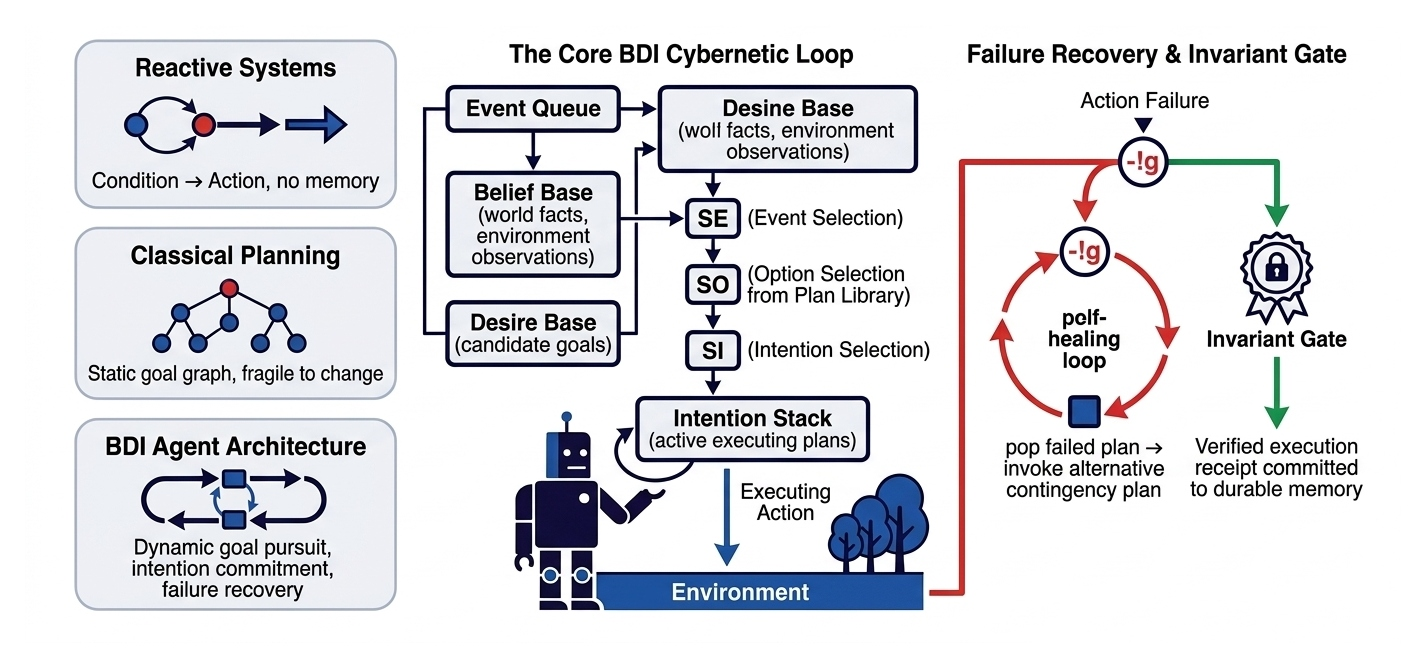
\includegraphics[width=\linewidth,height=8.0cm,keepaspectratio]{figures/fig-ch0-bdi-diagram.jpg}
    \end{minipage}
    \tcblower
    \begin{minipage}[t][2.0cm][t]{\linewidth}
      \pdgrotesk\scriptsize
      \textbf{\color{pderror!90!black} Artifact \& Limitation Audit:}\\
      \begin{itemize}[leftmargin=9pt,itemsep=0pt,topsep=0.5pt,parsep=0pt]
        \item Cluttered feedback loops with unreadable mathematical operators ($S_E, S_O, S_I$)
        \item Messy box corners, inconsistent padding, and illegible code snippets
        \item Non-standard color palette clashing with the rest of the volume
      \end{itemize}
    \end{minipage}
  \end{tcolorbox}
\end{minipage}\hfill
\begin{minipage}[t]{0.492\linewidth}
  \begin{tcolorbox}[
    colback=pdcobalt!3,colframe=pdcobalt!85!black,arc=1.5pt,
    boxrule=0.7pt,top=1.5pt,bottom=1.5pt,left=4pt,right=4pt,
    title={\pdgrotesk\footnotesize\bfseries \color{white} B. Authoritative Native Vector Replacement \hfill \texttt{.tex / TikZ / PGF}}
  ]
    \begin{minipage}[c][8.3cm][c]{\linewidth}
      \centering
      \sbox{\pdfigbox}{% fig-ch0-bdi-execution.tex
% BDI Execution Flow and Operational Choice Architecture
% 100% native vector Swiss TikZ layout adhering to Harbor Figure Standard (v2).
% Guaranteed collision-free panel architecture with bounded text containers.

% pd-robot-glyphs.tex
% Authentic vector robot glyphs and system iconography for Port Daddy architectural figures.
% Provides 100% vector replacements matching the AI-generated diagram prototypes.

\ifdefined\pdrobotglyphsloaded\else
\def\pdrobotglyphsloaded{1}

% -----------------------------------------------------------------------------
% 1. Standard Standing Agent Robot (Base Model)
% Args: shift (x,y), color, scale
% -----------------------------------------------------------------------------
\newcommand{\pdrobotbase}[3][1.0]{%
  \begin{scope}[shift={#2},scale=#1]
    % Head
    \draw[fill=#3!85, draw=#3!95!black, line width=0.6pt, rounded corners=2pt] (-0.28, 0.22) rectangle (0.28, 0.58);
    % Dual Antennae
    \draw[line width=0.65pt, draw=#3!95!black] (-0.12, 0.58) -- (-0.16, 0.72);
    \draw[line width=0.65pt, draw=#3!95!black] (0.12, 0.58) -- (0.16, 0.72);
    \fill[pdamber!90!orange] (-0.16, 0.72) circle (0.038);
    \fill[pdamber!90!orange] (0.16, 0.72) circle (0.038);
    % Screen / Visor
    \draw[fill=hhink!90, draw=none, rounded corners=1.2pt] (-0.22, 0.28) rectangle (0.22, 0.52);
    % Eyes
    \fill[pdteal!35!white] (-0.11, 0.40) circle (0.04);
    \fill[pdteal!35!white] (0.11, 0.40) circle (0.04);
    % Mouth bar
    \draw[pdteal!35!white, line width=0.4pt] (-0.07, 0.33) -- (0.07, 0.33);
    % Ear bolts
    \draw[fill=pdslate!60, draw=#3!95!black, line width=0.4pt] (-0.32, 0.35) rectangle (-0.28, 0.45);
    \draw[fill=pdslate!60, draw=#3!95!black, line width=0.4pt] (0.28, 0.35) rectangle (0.32, 0.45);
    % Neck
    \draw[fill=pdslate!70, draw=#3!95!black, line width=0.4pt] (-0.08, 0.16) rectangle (0.08, 0.22);
    % Body / Torso
    \draw[fill=#3!85, draw=#3!95!black, line width=0.6pt, rounded corners=2pt] (-0.32, -0.28) rectangle (0.32, 0.16);
    % Chest panel
    \draw[fill=pdpage, draw=#3!70!black, line width=0.35pt, rounded corners=1pt] (-0.22, -0.12) rectangle (0.22, 0.10);
    \fill[pdhealth] (-0.13, -0.01) circle (0.03);
    \fill[pdamber] (0.0, -0.01) circle (0.03);
    \fill[pderror] (0.13, -0.01) circle (0.03);
    % Arms
    \draw[fill=#3!75, draw=#3!95!black, line width=0.45pt, rounded corners=1.2pt] (-0.44, -0.20) rectangle (-0.32, 0.10);
    \draw[fill=#3!75, draw=#3!95!black, line width=0.45pt, rounded corners=1.2pt] (0.32, -0.20) rectangle (0.44, 0.10);
    % Legs & Feet
    \draw[fill=pdslate!80, draw=#3!95!black, line width=0.45pt] (-0.24, -0.46) rectangle (-0.09, -0.28);
    \draw[fill=pdslate!80, draw=#3!95!black, line width=0.45pt] (0.09, -0.46) rectangle (0.24, -0.28);
    \draw[fill=pdslate!90!black, draw=#3!95!black, line width=0.45pt, rounded corners=1pt] (-0.28, -0.52) rectangle (-0.05, -0.44);
    \draw[fill=pdslate!90!black, draw=#3!95!black, line width=0.45pt, rounded corners=1pt] (0.05, -0.52) rectangle (0.28, -0.44);
  \end{scope}
}

% -----------------------------------------------------------------------------
% 2. Robot Holding Voting / Lease Token Tablet
% -----------------------------------------------------------------------------
\newcommand{\pdrobottoken}[3][1.0]{%
  \begin{scope}[shift={#2},scale=#1]
    % Head
    \draw[fill=#3!85, draw=#3!95!black, line width=0.6pt, rounded corners=2pt] (-0.28, 0.22) rectangle (0.28, 0.58);
    % Antenna
    \draw[line width=0.65pt, draw=#3!95!black] (0, 0.58) -- (0, 0.73);
    \fill[pdamber!90!orange] (0, 0.73) circle (0.04);
    % Screen / Visor
    \draw[fill=hhink!90, draw=none, rounded corners=1.2pt] (-0.22, 0.28) rectangle (0.22, 0.52);
    \fill[pdteal!35!white] (-0.11, 0.40) circle (0.04);
    \fill[pdteal!35!white] (0.11, 0.40) circle (0.04);
    \draw[pdteal!35!white, line width=0.4pt] (-0.07, 0.33) -- (0.07, 0.33);
    % Neck
    \draw[fill=pdslate!70, draw=#3!95!black, line width=0.4pt] (-0.08, 0.16) rectangle (0.08, 0.22);
    % Body
    \draw[fill=#3!85, draw=#3!95!black, line width=0.6pt, rounded corners=2pt] (-0.32, -0.28) rectangle (0.32, 0.16);
    % Legs & Feet
    \draw[fill=pdslate!80, draw=#3!95!black, line width=0.45pt] (-0.24, -0.46) rectangle (-0.09, -0.28);
    \draw[fill=pdslate!80, draw=#3!95!black, line width=0.45pt] (0.09, -0.46) rectangle (0.24, -0.28);
    \draw[fill=pdslate!90!black, draw=#3!95!black, line width=0.45pt, rounded corners=1pt] (-0.28, -0.52) rectangle (-0.05, -0.44);
    \draw[fill=pdslate!90!black, draw=#3!95!black, line width=0.45pt, rounded corners=1pt] (0.05, -0.52) rectangle (0.28, -0.44);
    % Arms holding tablet
    \draw[fill=#3!75, draw=#3!95!black, line width=0.45pt] (-0.42, -0.08) -- (-0.22, 0.05) -- (-0.18, 0.0) -- (-0.35, -0.13) -- cycle;
    \draw[fill=#3!75, draw=#3!95!black, line width=0.45pt] (0.42, -0.08) -- (0.22, 0.05) -- (0.18, 0.0) -- (0.35, -0.13) -- cycle;
    % Tablet
    \draw[fill=pdpage, draw=pdcobalt, line width=0.55pt, rounded corners=1.2pt] (-0.24, -0.18) rectangle (0.24, 0.18);
    \node[font=\fontsize{3.8}{4.5}\selectfont\bfseries\color{pdcobalt}] at (0, 0.06) {VOTING};
    \node[font=\fontsize{3.5}{4.2}\selectfont\bfseries\color{hhink}] at (0, -0.06) {TOKEN};
  \end{scope}
}

% -----------------------------------------------------------------------------
% 3. Robot at Laptop / Deliberation
% -----------------------------------------------------------------------------
\newcommand{\pdrobotlaptop}[3][1.0]{%
  \begin{scope}[shift={#2},scale=#1]
    % Head (Tilted slightly forward)
    \draw[fill=#3!85, draw=#3!95!black, line width=0.6pt, rounded corners=2pt] (-0.26, 0.22) rectangle (0.26, 0.56);
    % Dual Antennae
    \draw[line width=0.65pt, draw=#3!95!black] (-0.10, 0.56) -- (-0.14, 0.70);
    \draw[line width=0.65pt, draw=#3!95!black] (0.10, 0.56) -- (0.14, 0.70);
    \fill[pdteal] (-0.14, 0.70) circle (0.038);
    \fill[pdteal] (0.14, 0.70) circle (0.038);
    % Visor
    \draw[fill=hhink!90, draw=none, rounded corners=1.2pt] (-0.20, 0.28) rectangle (0.20, 0.50);
    \fill[pdteal!40!white] (-0.10, 0.38) circle (0.038);
    \fill[pdteal!40!white] (0.10, 0.38) circle (0.038);
    % Body
    \draw[fill=#3!85, draw=#3!95!black, line width=0.6pt, rounded corners=2pt] (-0.30, -0.26) rectangle (0.30, 0.18);
    % Legs (Seated)
    \draw[fill=pdslate!80, draw=#3!95!black, line width=0.45pt] (-0.25, -0.38) rectangle (0.25, -0.26);
    % Desk surface
    \draw[line width=1.0pt, pdslate!80!black] (-0.6, -0.38) -- (0.7, -0.38);
    % Laptop Base
    \draw[fill=pdslate!40, draw=pdslate!90!black, line width=0.45pt] (-0.05, -0.38) -- (0.50, -0.38) -- (0.46, -0.33) -- (-0.02, -0.33) -- cycle;
    % Laptop Screen
    \draw[fill=pdcobalt!90!black, draw=pdslate!90!black, line width=0.5pt, rounded corners=1pt] (0.42, -0.33) -- (0.52, 0.05) -- (0.15, 0.05) -- (0.08, -0.33) -- cycle;
    % Glowing Screen Text
    \draw[pdteal!50!white, line width=0.4pt] (0.18, -0.03) -- (0.42, -0.03);
    \draw[pdteal!50!white, line width=0.4pt] (0.16, -0.12) -- (0.38, -0.12);
    \draw[pdteal!50!white, line width=0.4pt] (0.14, -0.21) -- (0.34, -0.21);
    % Arms on keyboard
    \draw[fill=#3!75, draw=#3!95!black, line width=0.45pt] (-0.22, 0.05) to[out=-20,in=160] (0.12, -0.30) -- (0.18, -0.33) -- (-0.18, -0.05) -- cycle;
  \end{scope}
}

% -----------------------------------------------------------------------------
% 4. Red-and-White Disablement Barrier
% -----------------------------------------------------------------------------
\newcommand{\pdbarrierline}[4]{% (x1, y1) to (x2, y2)
  \draw[line width=4.5pt, white] (#1,#2) -- (#3,#4);
  \draw[line width=4.5pt, pderror, dashed, dash pattern=on 6pt off 6pt] (#1,#2) -- (#3,#4);
  \draw[line width=0.6pt, pderror!80!black] (#1,#2) -- (#3,#4);
}

% -----------------------------------------------------------------------------
% 5. Vector Iconography Definitions
% -----------------------------------------------------------------------------
% Crossed Tools (Wrench + Screwdriver)
\newcommand{\pdicontools}[2][1.0]{%
  \begin{scope}[shift={#2},scale=#1]
    \draw[line width=1.4pt, pdslate!80!black, line cap=round] (-0.25,-0.25) -- (0.25,0.25);
    \draw[line width=1.4pt, pdrust!90!black, line cap=round] (-0.25,0.25) -- (0.25,-0.25);
    \draw[fill=pdslate!90!black, line width=0.4pt] (0.18,0.18) circle (0.10);
    \fill[white] (0.20,0.20) circle (0.04);
    \draw[fill=pdrust!90!black, line width=0.4pt] (0.20,-0.22) rectangle (0.26,-0.16);
  \end{scope}
}

% Git Branch
\newcommand{\pdicongit}[2][1.0]{%
  \begin{scope}[shift={#2},scale=#1]
    \draw[line width=1.1pt, pdteal!90!black] (0,-0.32) -- (0,0.32);
    \draw[line width=1.1pt, pdteal!90!black] (0,-0.08) to[out=45,in=180] (0.24,0.16);
    \fill[pdteal!90!black] (0,-0.24) circle (0.06);
    \fill[pdteal!90!black] (0,0.24) circle (0.06);
    \fill[pdteal!90!black] (0.24,0.16) circle (0.06);
  \end{scope}
}

% Network Globe
\newcommand{\pdiconglobe}[2][1.0]{%
  \begin{scope}[shift={#2},scale=#1]
    \draw[line width=0.7pt, pdcobalt!85!black] (0,0) circle (0.28);
    \draw[line width=0.5pt, pdcobalt!70] (0,0) ellipse (0.13 and 0.28);
    \draw[line width=0.5pt, pdcobalt!70] (-0.28,0) -- (0.28,0);
    \draw[line width=0.5pt, pdcobalt!70] (-0.24,0.14) -- (0.24,0.14);
    \draw[line width=0.5pt, pdcobalt!70] (-0.24,-0.14) -- (0.24,-0.14);
  \end{scope}
}

% Host OS Gear / Process
\newcommand{\pdicongear}[2][1.0]{%
  \begin{scope}[shift={#2},scale=#1]
    \fill[pdslate!75!black] (0,0) circle (0.22);
    \foreach \a in {0,45,90,135,180,225,270,315} {
      \fill[pdslate!75!black] (\a:0.26) circle (0.055);
    }
    \fill[white] (0,0) circle (0.09);
  \end{scope}
}

% Stopwatch / Timer
\newcommand{\pdicontimer}[2][1.0]{%
  \begin{scope}[shift={#2},scale=#1]
    \draw[line width=0.75pt, pdamber!90!black] (0,0) circle (0.25);
    \draw[line width=0.8pt, pdamber!90!black] (0,0.25) -- (0,0.33);
    \draw[line width=1.0pt, pdamber!90!black] (-0.06,0.33) -- (0.06,0.33);
    \draw[line width=0.75pt, pdamber!90!black] (0,0) -- (0,0.14);
    \draw[line width=0.75pt, pdamber!90!black] (0,0) -- (0.11,0.05);
    \fill[pdamber!90!black] (0,0) circle (0.035);
  \end{scope}
}

% Hardware Crash / Lightning Burst
\newcommand{\pdiconcrash}[2][1.0]{%
  \begin{scope}[shift={#2},scale=#1]
    \fill[pderror!90!black] (0.06,0.32) -- (-0.12,0.04) -- (-0.02,0.04) -- (-0.14,-0.32) -- (0.12,-0.02) -- (0.02,-0.02) -- cycle;
  \end{scope}
}

% Shield with Checkmark
\newcommand{\pdiconshieldcheck}[2][1.0]{%
  \begin{scope}[shift={#2},scale=#1]
    \fill[pdcobalt!90!black] (0,0.32) -- (0.26,0.20) to[out=-70,in=45] (0,-0.32) to[out=135,in=-110] (-0.26,0.20) -- cycle;
    \draw[line width=1.1pt, white, line cap=round, line join=round] (-0.11,-0.02) -- (-0.03,-0.12) -- (0.13,0.10);
  \end{scope}
}

% Padlock
\newcommand{\pdiconlock}[2][1.0]{%
  \begin{scope}[shift={#2},scale=#1]
    % Shackle
    \draw[line width=0.9pt, pdslate!80!black] (-0.12,0.05) -- (-0.12,0.18) arc (180:0:0.12) -- (0.12,0.05);
    % Body
    \draw[fill=pderror!85!black, draw=pderror!95!black, line width=0.5pt, rounded corners=1pt] (-0.18,-0.20) rectangle (0.18,0.06);
    % Keyhole
    \fill[white] (0,-0.04) circle (0.035);
    \draw[line width=0.6pt, white] (0,-0.04) -- (0,-0.13);
  \end{scope}
}

% Speedometer / Spend Cap
\newcommand{\pdiconspeedometer}[2][1.0]{%
  \begin{scope}[shift={#2},scale=#1]
    \draw[line width=1.0pt, pdteal!90!black] (-0.28,-0.04) arc (180:40:0.28);
    \draw[line width=1.0pt, pderror] (40:0.28) arc (40:0:0.28);
    \draw[line width=0.8pt, hhink, line cap=round] (0,-0.04) -- (0.12,0.14);
    \fill[hhink] (0,-0.04) circle (0.05);
  \end{scope}
}

% Sparkle Broom / Hygiene Wand
\newcommand{\pdiconbroom}[2][1.0]{%
  \begin{scope}[shift={#2},scale=#1]
    \draw[line width=1.2pt, pdteal!90!black, line cap=round] (-0.2,-0.2) -- (0.15,0.15);
    % Sparkles
    \fill[pdamber!90!orange] (0.22,0.22) circle (0.04);
    \fill[pdteal] (0.05,0.26) circle (0.03);
    \fill[pdteal] (0.26,0.05) circle (0.03);
  \end{scope}
}

% Host Terminal Substrate
\newcommand{\pdiconterminal}[2][1.0]{%
  \begin{scope}[shift={#2},scale=#1]
    \draw[fill=hhink!95, draw=pdslate!80, line width=0.6pt, rounded corners=1.5pt] (-0.35,-0.25) rectangle (0.35,0.25);
    \draw[fill=pderror] (-0.26,0.18) circle (0.025);
    \fill[pdamber] (-0.18,0.18) circle (0.025);
    \fill[pdhealth] (-0.10,0.18) circle (0.025);
    \node[font=\fontsize{4.5}{5}\selectfont\ttfamily\color{pdhealth}] at (0,-0.05) {>\_};
  \end{scope}
}

% Coins Stack
\newcommand{\pdiconcoins}[2][1.0]{%
  \begin{scope}[shift={#2},scale=#1]
    \foreach \y in {-0.24, -0.12, 0.0, 0.12} {
      \draw[fill=pdamber!80!orange, draw=pdamber!95!black, line width=0.45pt] (0,\y) ellipse (0.24 and 0.07);
    }
  \end{scope}
}

% Tall Coins Stack
\newcommand{\pdiconcoinstall}[2][1.0]{%
  \begin{scope}[shift={#2},scale=#1]
    \foreach \y in {-0.30, -0.18, -0.06, 0.06, 0.18, 0.30} {
      \draw[fill=pdamber!80!orange, draw=pdamber!95!black, line width=0.45pt] (0,\y) ellipse (0.24 and 0.07);
    }
  \end{scope}
}

% Slashed Coins (Stake Slashed)
\newcommand{\pdiconcoinslashed}[2][1.0]{%
  \begin{scope}[shift={#2},scale=#1]
    \foreach \y in {-0.20, -0.08, 0.04, 0.16} {
      \draw[fill=pdamber!70!white, draw=pdamber!80!black, line width=0.45pt] (0,\y) ellipse (0.22 and 0.065);
    }
    \draw[line width=1.5pt, pderror, line cap=round] (-0.26,-0.24) -- (0.26,0.24);
  \end{scope}
}

% Magnifying Glass (Audit Inspection)
\newcommand{\pdiconmagnifier}[2][1.0]{%
  \begin{scope}[shift={#2},scale=#1]
    \draw[line width=0.9pt, pdteal!90!black] (0,0.06) circle (0.16);
    \draw[line width=1.4pt, pdteal!90!black, line cap=round] (0.12,-0.06) -- (0.26,-0.20);
    \fill[white] (-0.04,0.10) circle (0.04);
  \end{scope}
}

% Arbitration Gavel & Scales of Justice
\newcommand{\pdiconarbitration}[2][1.0]{%
  \begin{scope}[shift={#2},scale=#1]
    % Central post
    \draw[line width=0.8pt, pdrust!90!black] (0.15,-0.20) -- (0.15,0.22);
    \draw[line width=0.8pt, pdrust!90!black] (-0.05,0.18) -- (0.35,0.18);
    \draw[line width=0.5pt, pdrust!80] (-0.05,0.18) -- (-0.12,0.02) -- (0.02,0.02) -- cycle;
    \draw[line width=0.5pt, pdrust!80] (0.35,0.18) -- (0.28,0.02) -- (0.42,0.02) -- cycle;
    % Gavel
    \draw[line width=1.4pt, pdrust!95!black, line cap=round] (-0.30,-0.18) -- (-0.10,0.05);
    \draw[fill=pdrust!90!black, draw=pdrust!95!black, line width=0.5pt, rounded corners=1pt] (-0.22,0.0) -- (-0.12,0.12) -- (-0.02,0.04) -- (-0.12,-0.08) -- cycle;
  \end{scope}
}

% Cash Bill / Liquidated Damages
\newcommand{\pdiconcash}[2][1.0]{%
  \begin{scope}[shift={#2},scale=#1]
    \draw[fill=white, draw=pdslate!90!black, line width=0.6pt, rounded corners=1.5pt] (-0.35,-0.20) rectangle (0.35,0.20);
    \draw[line width=0.5pt, pdteal!80!black] (-0.28,-0.14) rectangle (0.28,0.14);
    \fill[pdteal!90!black] (0,0) circle (0.08);
    \fill[pdteal!90!black] (-0.22,0) circle (0.035);
    \fill[pdteal!90!black] (0.22,0) circle (0.035);
  \end{scope}
}

% Group of People / Remedy
\newcommand{\pdicongrouppeople}[2][1.0]{%
  \begin{scope}[shift={#2},scale=#1]
    % Center person
    \fill[hhink] (0,0.12) circle (0.09);
    \fill[hhink] (-0.15,-0.20) to[out=70,in=180] (0,-0.02) to[out=0,in=110] (0.15,-0.20) -- cycle;
    % Left person
    \fill[hhgray!90!black] (-0.22,0.06) circle (0.075);
    \fill[hhgray!90!black] (-0.34,-0.20) to[out=70,in=180] (-0.22,-0.06) to[out=0,in=110] (-0.10,-0.20) -- cycle;
    % Right person
    \fill[hhgray!90!black] (0.22,0.06) circle (0.075);
    \fill[hhgray!90!black] (0.10,-0.20) to[out=70,in=180] (0.22,-0.06) to[out=0,in=110] (0.34,-0.20) -- cycle;
  \end{scope}
}

% Database Cylinder
\newcommand{\pdicondatabase}[2][1.0]{%
  \begin{scope}[shift={#2},scale=#1]
    \draw[fill=pdslate!20, draw=pdslate!90!black, line width=0.6pt] (-0.25,-0.15) rectangle (0.25,0.15);
    \draw[fill=pdslate!30, draw=pdslate!90!black, line width=0.5pt] (0,0.15) ellipse (0.25 and 0.08);
    \draw[draw=pdslate!90!black, line width=0.5pt] (-0.25,0) arc (180:360:0.25 and 0.08);
    \draw[draw=pdslate!90!black, line width=0.5pt] (-0.25,-0.15) arc (180:360:0.25 and 0.08);
  \end{scope}
}

% Signed Document / Witness Receipts
\newcommand{\pdicondocument}[2][1.0]{%
  \begin{scope}[shift={#2},scale=#1]
    \draw[fill=white, draw=pdslate!90!black, line width=0.55pt] (-0.18,-0.24) -- (0.10,-0.24) -- (0.18,-0.16) -- (0.18,0.24) -- (-0.18,0.24) -- cycle;
    \draw[draw=pdslate!80, line width=0.45pt] (0.10,-0.24) -- (0.10,-0.16) -- (0.18,-0.16);
    \draw[pdslate!70, line width=0.4pt] (-0.12,0.16) -- (0.12,0.16);
    \draw[pdslate!70, line width=0.4pt] (-0.12,0.08) -- (0.12,0.08);
    \draw[pdslate!70, line width=0.4pt] (-0.12,0.00) -- (0.06,0.00);
    % Feather / quill
    \draw[line width=0.7pt, pdcobalt!80!black] (0.08,-0.12) to[out=45,in=-45] (0.24,0.06);
  \end{scope}
}

% Merkle Inclusion Proof Tree
\newcommand{\pdiconmerkle}[2][1.0]{%
  \begin{scope}[shift={#2},scale=#1]
    % Root
    \draw[line width=0.5pt, pdslate!80] (0,0.20) -- (-0.16,0.04);
    \draw[line width=0.5pt, pdslate!80] (0,0.20) -- (0.16,0.04);
    \draw[line width=0.5pt, pdslate!80] (-0.16,0.04) -- (-0.24,-0.14);
    \draw[line width=0.5pt, pdslate!80] (-0.16,0.04) -- (-0.08,-0.14);
    \draw[line width=0.5pt, pdslate!80] (0.16,0.04) -- (0.08,-0.14);
    \draw[line width=0.5pt, pdslate!80] (0.16,0.04) -- (0.24,-0.14);
    \draw[fill=white, draw=pdslate!90!black, line width=0.4pt] (-0.05,0.16) rectangle (0.05,0.24);
    \draw[fill=white, draw=pdslate!90!black, line width=0.4pt] (-0.20,0.0) rectangle (-0.12,0.08);
    \draw[fill=white, draw=pdslate!90!black, line width=0.4pt] (0.12,0.0) rectangle (0.20,0.08);
    \draw[fill=pdteal!80!white, draw=pdteal!95!black, line width=0.5pt] (-0.28,-0.18) rectangle (-0.20,-0.10);
    \draw[fill=white, draw=pdslate!90!black, line width=0.4pt] (-0.12,-0.18) rectangle (-0.04,-0.10);
    \draw[fill=white, draw=pdslate!90!black, line width=0.4pt] (0.04,-0.18) rectangle (0.12,-0.10);
    \draw[fill=white, draw=pdslate!90!black, line width=0.4pt] (0.20,-0.18) rectangle (0.28,-0.10);
  \end{scope}
}

% Key (Cryptographic Key / Capability Key)
\newcommand{\pdiconkey}[2][1.0]{%
  \begin{scope}[shift={#2},scale=#1]
    \draw[line width=0.8pt, pdamber!95!black] (0, 0.12) circle (0.14);
    \fill[white] (0, 0.12) circle (0.06);
    \draw[line width=0.85pt, pdamber!95!black] (0, -0.02) -- (0, -0.26);
    \draw[line width=0.7pt, pdamber!95!black] (0, -0.14) -- (0.10, -0.14);
    \draw[line width=0.7pt, pdamber!95!black] (0, -0.22) -- (0.08, -0.22);
  \end{scope}
}

\def\pdiconclock{\pdicontimer}
\def\pdiconlightning{\pdiconcrash}

\fi

\pdfigurehue{pdcobalt}%
\begin{tikzpicture}[pd figure,x=1cm,y=1cm]
  \tikzset{
    containerbox/.style={
      draw=pdslate!40,
      line width=0.75pt,
      fill=white,
      rounded corners=3pt
    },
    innercard/.style={
      draw=pdslate!30,
      line width=0.55pt,
      fill=hhpaper!30,
      rounded corners=2pt,
      inner sep=3pt
    },
    flowarrow/.style={
      draw=pdcobalt,
      line width=0.8pt,
      ->,
      >=Stealth
    },
    feedbackarrow/.style={
      draw=pdteal!80!black,
      line width=0.8pt,
      ->,
      >=Stealth
    }
  }

  % =========================================================================
  % PANEL 1: PARADIGM SPECTRUM (Left: x in [0.1, 4.1], y in [0.4, 5.5])
  % =========================================================================
  \draw[containerbox] (0.1, 0.4) rectangle (4.1, 5.5);
  \fill[fill=pdslate!85!black, rounded corners=2pt] (0.14, 5.12) rectangle (4.06, 5.46);
  \node[anchor=center] at (2.1, 5.29) {%
    \fontsize{5.2}{6.2}\selectfont\bfseries\color{white}PARADIGM SPECTRUM%
  };

  % Card 1.1: Reactive Systems
  \begin{scope}[shift={(0.3, 3.8)}]
    \draw[innercard] (0, 0) rectangle (3.5, 1.15);
    \node[anchor=north west, font=\fontsize{4.8}{5.8}\selectfont\bfseries\color{hhink}] at (0.15, 1.05) {1. Reactive Systems};
    % diagram
    \fill[pdslate!40] (0.45, 0.62) circle (0.11cm);
    \draw[->, line width=0.6pt, pdslate!80] (0.65, 0.62) -- (1.25, 0.62);
    \fill[pdslate!80, rounded corners=1pt] (1.35, 0.51) rectangle (1.95, 0.73);
    \node[anchor=north west, font=\fontsize{3.8}{4.6}\selectfont\color{hhgray!90!black}, text width=3.2cm] at (0.15, 0.42) {%
      Stateless Condition $\rightarrow$ Action mapping. Fast reflex, blind to future consequences.%
    };
  \end{scope}

  % Card 1.2: Classical Planning
  \begin{scope}[shift={(0.3, 2.3)}]
    \draw[innercard] (0, 0) rectangle (3.5, 1.35);
    \node[anchor=north west, font=\fontsize{4.8}{5.8}\selectfont\bfseries\color{hhink}] at (0.15, 1.25) {2. Classical Planning};
    % graph (lowered to avoid title)
    \fill[pdteal!70] (0.45, 0.68) circle (0.07cm);
    \draw[line width=0.5pt, pdteal] (0.45, 0.68) -- (0.95, 0.81) circle (0.06cm);
    \draw[line width=0.5pt, pdteal] (0.45, 0.68) -- (0.95, 0.55) circle (0.06cm);
    \draw[line width=0.5pt, pdteal] (0.95, 0.81) -- (1.55, 0.81) circle (0.06cm);
    \node[anchor=north west, font=\fontsize{3.8}{4.6}\selectfont\color{hhgray!90!black}, text width=3.2cm] at (0.15, 0.46) {%
      Static state-space search (STRIPS/PDDL). Full precomputation; brittle when state diverges.%
    };
  \end{scope}

  % Card 1.3: BDI Architecture
  \begin{scope}[shift={(0.3, 0.55)}]
    \draw[draw=pdcobalt!80, line width=0.75pt, fill=pdcobalt!6, rounded corners=2pt] (0, 0) rectangle (3.5, 1.6);
    \node[anchor=north west, font=\fontsize{5.0}{6.0}\selectfont\bfseries\color{pdcobalt}] at (0.15, 1.48) {3. BDI Cybernetic Agent};
    % loop icon (lowered to avoid title)
    \draw[->, line width=0.65pt, pdcobalt] (0.5, 0.95) to[out=50, in=130] (1.5, 0.95);
    \draw[->, line width=0.65pt, pdcobalt] (1.5, 0.80) to[out=-130, in=-50] (0.5, 0.80);
    \node[anchor=north west, font=\fontsize{3.8}{4.6}\selectfont\color{hhink}, text width=3.2cm] at (0.15, 0.68) {%
      Dynamic commitment to intentions, practical reasoning ($S_E, S_O, S_I$), continuous perception, and built-in failure recovery.%
    };
  \end{scope}

  % =========================================================================
  % PANEL 2: THE CORE BDI CYBERNETIC LOOP (Center: x in [4.3, 10.3])
  % =========================================================================
  \draw[containerbox] (4.3, 0.4) rectangle (10.3, 5.5);
  \fill[fill=pdcobalt!90!black, rounded corners=2pt] (4.34, 5.12) rectangle (10.26, 5.46);
  \node[anchor=center] at (7.3, 5.29) {%
    \fontsize{5.2}{6.2}\selectfont\bfseries\color{white}THE CORE BDI CYBERNETIC LOOP%
  };

  % Row 1: Event Queue, Belief Base, Desire Base
  % Event Queue (Left)
  \begin{scope}[shift={(5.4, 4.45)}]
    \draw[draw=pdcobalt, fill=white, line width=0.6pt, rounded corners=2pt] (-0.85, -0.32) rectangle (0.85, 0.32);
    \node[font=\fontsize{4.6}{5.5}\selectfont\bfseries\color{pdcobalt}, align=center] at (0, 0) {Event Queue ($E$)\\{\fontsize{3.6}{4.4}\selectfont external / internal}};
  \end{scope}

  % Desire Base (Right)
  \begin{scope}[shift={(9.2, 4.45)}]
    \draw[draw=pdcobalt, fill=white, line width=0.6pt, rounded corners=2pt] (-0.85, -0.32) rectangle (0.85, 0.32);
    \node[font=\fontsize{4.6}{5.5}\selectfont\bfseries\color{pdcobalt}, align=center] at (0, 0) {Desire Base ($D$)\\{\fontsize{3.6}{4.4}\selectfont candidate goals}};
  \end{scope}

  % Belief Base (Center Left)
  \begin{scope}[shift={(5.4, 3.45)}]
    \draw[draw=pdcobalt, fill=white, line width=0.6pt, rounded corners=2pt] (-0.85, -0.35) rectangle (0.85, 0.35);
    \node[font=\fontsize{4.6}{5.5}\selectfont\bfseries\color{pdcobalt}, align=center] at (0, 0) {Belief Base ($B$)\\{\fontsize{3.6}{4.4}\selectfont world facts \& obs}};
  \end{scope}

  % Selection Functions Stack (Center Right)
  \begin{scope}[shift={(8.3, 3.45)}]
    \draw[draw=pdslate!40, fill=hhpaper!40, rounded corners=2pt] (-1.7, -0.55) rectangle (1.7, 0.55);
    % SE
    \draw[fill=pdcobalt!15, draw=pdcobalt, line width=0.45pt, rounded corners=1.5pt] (-1.55, 0.20) rectangle (1.55, 0.46);
    \node[font=\fontsize{4.0}{4.8}\selectfont\bfseries\color{pdcobalt}] at (0, 0.33) {$S_E$: Event Selection Function};
    % SO
    \draw[fill=pdteal!15, draw=pdteal, line width=0.45pt, rounded corners=1.5pt] (-1.55, -0.13) rectangle (1.55, 0.13);
    \node[font=\fontsize{4.0}{4.8}\selectfont\bfseries\color{pdteal!90!black}] at (0, 0) {$S_O$: Option / Plan Selection Function};
    % SI
    \draw[fill=pdindigo!15, draw=pdindigo, line width=0.45pt, rounded corners=1.5pt] (-1.55, -0.46) rectangle (1.55, -0.20);
    \node[font=\fontsize{4.0}{4.8}\selectfont\bfseries\color{pdindigo!90!black}] at (0, -0.33) {$S_I$: Intention Selection Function};
  \end{scope}

  % Connections from E, B, D into Selection Functions
  \draw[flowarrow] (5.4, 4.13) -- (5.4, 3.8);
  \draw[flowarrow] (6.25, 4.45) -- (6.6, 3.7);
  \draw[flowarrow] (6.25, 3.45) -- (6.6, 3.45);
  \draw[flowarrow] (8.5, 4.13) to[out=-90, in=60] (8.3, 4.0);

  % Intention Stack (active executing plans)
  \begin{scope}[shift={(7.3, 2.15)}]
    \draw[draw=pdcobalt!90!black, fill=pdcobalt!10, line width=0.75pt, rounded corners=2pt] (-2.2, -0.35) rectangle (2.2, 0.35);
    \node[font=\fontsize{4.6}{5.5}\selectfont\bfseries\color{pdcobalt}, align=center] at (0, 0.10) {Intention Stack ($I$)};
    \node[font=\fontsize{3.6}{4.4}\selectfont\color{hhink}, align=center] at (0, -0.14) {Active committed plans awaiting execution};
  \end{scope}

  \draw[flowarrow] (8.3, 2.9) -- (7.8, 2.5);

  % Downward Action Dispatch
  \draw[flowarrow, line width=0.9pt] (7.3, 1.8) -- (7.3, 1.25);
  \node[anchor=west, font=\fontsize{4.0}{4.8}\selectfont\bfseries\color{pdcobalt}] at (7.35, 1.55) {Execute Action $a \in \pi$};

  % Robot Worker + Environment Box
  \begin{scope}[shift={(5.9, 0.85)}]
    \pdrobotbase[0.55]{(0, 0)}{pdcobalt}
  \end{scope}

  \begin{scope}[shift={(7.8, 0.85)}]
    \draw[fill=pdslate!90!black, draw=none, rounded corners=2pt] (-1.1, -0.28) rectangle (1.1, 0.28);
    \node[font=\fontsize{4.8}{5.8}\selectfont\bfseries\color{white}] at (0, 0) {Host Environment};
  \end{scope}

  % Perception Feedback Loop: strictly within Center Panel, running up at x=4.6
  \draw[feedbackarrow] (6.7, 0.85) -- (5.9, 0.85);
  \draw[feedbackarrow] (5.3, 0.85) to[out=180, in=-90] (4.62, 1.8) -- (4.62, 3.1) to[out=90, in=180] (5.4, 3.45);
  \node[anchor=center, font=\fontsize{3.5}{4.2}\selectfont\bfseries\color{pdteal!90!black}, fill=white, inner sep=1pt, rotate=90] at (4.62, 2.45) {Perceptions ($P$)};

  % =========================================================================
  % PANEL 3: FAILURE RECOVERY & INVARIANT GATE (Right: x in [10.5, 14.5])
  % =========================================================================
  \draw[containerbox] (10.5, 0.4) rectangle (14.5, 5.5);
  \fill[fill=pdslate!85!black, rounded corners=2pt] (10.54, 5.12) rectangle (14.46, 5.46);
  \node[anchor=center] at (12.5, 5.29) {%
    \fontsize{5.2}{6.2}\selectfont\bfseries\color{white}FAILURE RECOVERY \& GATE%
  };

  % Top: Outcome Evaluator
  \begin{scope}[shift={(12.5, 4.5)}]
    \draw[draw=pdslate!60, fill=hhpaper!40, line width=0.6pt, rounded corners=2pt] (-1.5, -0.32) rectangle (1.5, 0.32);
    \node[font=\fontsize{4.6}{5.5}\selectfont\bfseries\color{hhink}] at (0, 0) {Action Result Evaluator};
  \end{scope}

  % Link from Center Panel Environment to Right Panel Evaluator via clean vertical channel
  \draw[flowarrow, dashed] (8.9, 0.85) -- (10.4, 0.85) -- (10.4, 4.5) -- (11.0, 4.5);

  % Branch 1: Action Failure (-!g)
  \begin{scope}[shift={(11.45, 3.3)}]
    \draw[fill=pderror, draw=none] (0, 0) circle (0.24cm);
    \node[font=\fontsize{5.2}{6.2}\selectfont\bfseries\color{white}] at (0, 0) {-!g};
    \node[anchor=north, font=\fontsize{4.0}{4.8}\selectfont\bfseries\color{pderror}, align=center] at (0, -0.28) {%
      Failure Event\\Trigger%
    };
  \end{scope}

  % Branch 2: Invariant Gate (Success)
  \begin{scope}[shift={(13.55, 3.3)}]
    \draw[draw=pdhealth!90!black, fill=pdhealth!10, line width=0.75pt, rounded corners=2pt] (-0.55, -0.32) rectangle (0.55, 0.32);
    \pdiconlock[0.55]{(0, 0)}
    \node[anchor=north, font=\fontsize{4.0}{4.8}\selectfont\bfseries\color{pdhealth!90!black}, align=center] at (0, -0.36) {%
      Invariant Gate\\Verification%
    };
  \end{scope}

  \draw[->, line width=0.75pt, pderror] (12.0, 4.18) to[out=-120, in=90] (11.45, 3.6);
  \draw[->, line width=0.75pt, pdhealth!90!black] (13.0, 4.18) to[out=-60, in=90] (13.55, 3.65);

  % Failure Healing Action
  \begin{scope}[shift={(11.45, 1.4)}]
    \draw[draw=pderror!60, fill=pderror!6, line width=0.5pt, rounded corners=2pt] (-0.85, -0.55) rectangle (0.85, 0.55);
    \node[font=\fontsize{3.8}{4.6}\selectfont\color{hhink}, align=center, text width=1.5cm] at (0, 0) {%
      Pop failed plan\\from stack $\rightarrow$\\invoke alternative\\contingency plan%
    };
  \end{scope}
  \draw[->, line width=0.65pt, pderror] (11.45, 2.3) -- (11.45, 1.95);

  % Success Durable Memory Commit
  \begin{scope}[shift={(13.55, 1.4)}]
    \draw[draw=pdhealth!60, fill=pdhealth!6, line width=0.5pt, rounded corners=2pt] (-0.85, -0.55) rectangle (0.85, 0.55);
    \node[font=\fontsize{3.8}{4.6}\selectfont\bfseries\color{pdhealth!90!black}, align=center, text width=1.5cm] at (0, 0) {%
      Execution receipt\\cryptographically\\signed \& committed\\to durable memory%
    };
  \end{scope}
  \draw[->, line width=0.65pt, pdhealth!90!black] (13.55, 2.3) -- (13.55, 1.95);

\end{tikzpicture}
}
      \pdautoscale{8.0cm}{\linewidth}
    \end{minipage}
    \tcblower
    \begin{minipage}[t][2.0cm][t]{\linewidth}
      \pdgrotesk\scriptsize
      \textbf{{\color{pdcobalt} Engineering \& Typography Guarantees:}}\\
      \begin{itemize}[leftmargin=9pt,itemsep=0pt,topsep=0.5pt,parsep=0pt]
        \item 3 clear architectural swimlanes: 1. Perception \& Events, 2. Plan Deliberation, 3. Intention Execution
        \item Formal AgentSpeak(L) selection functions ($S_E, S_O, S_I$) with recovery event ($-!g$)
        \item Strict Swiss styling using pdcobalt, pdteal, and pdindigo with 4pt inner padding
      \end{itemize}
    \end{minipage}
  \end{tcolorbox}
\end{minipage}

\vspace*{0.05cm}
\noindent
\begin{tcolorbox}[
  colback=hhpaper,colframe=hhgray!35,arc=1.5pt,boxrule=0.4pt,
  top=1.5pt,bottom=1.5pt,left=6pt,right=6pt
]
  \pdgrotesk\scriptsize
  \noindent
  \textbf{Visual Substrate:} Lossy Bitmap Raster $\rightarrow$ \textbf{\color{pdcobalt}Native PDF / PostScript Vector}\hfill
  \textbf{Text Engine:} Pixelated Approximations $\rightarrow$ \textbf{\color{pdcobalt}Book Typography (OpenType)}\hfill
  \textbf{Resolution:} Fixed DPI Limit $\rightarrow$ \textbf{\color{pdcobalt}Infinite Resolution ($\infty$)}\hfill
  \textbf{Status:} \textbf{\color{pdteal}RECONCILED \& VERIFIED}
\end{tcolorbox}
\clearpage

% =========================================================================
% PAGE 10: Figure 0.10
% =========================================================================
\noindent
\begin{minipage}[t]{\linewidth}
  \noindent{\pdgrotesk\large\bfseries Figure 0.10 \textperiodcentered\ Concurrency Foundations: Virtual Actors vs. CSP Rendezvous}\hfill
  {\pdgrotesk\footnotesize\color{hhgray} Section 0.1.4 · Concurrency \& Message Passing · Hewitt-Agha vs. Hoare CSP}\\
  \vspace*{0.03cm}
  \noindent{\color{hhgray!40}\rule{\linewidth}{0.5pt}}
\end{minipage}

\vspace*{0.05cm}
\noindent
\begin{minipage}[t]{0.492\linewidth}
  \begin{tcolorbox}[
    colback=pdslate!4,colframe=pdslate!70!black,arc=1.5pt,
    boxrule=0.6pt,top=1.5pt,bottom=1.5pt,left=4pt,right=4pt,
    title={\pdgrotesk\footnotesize\bfseries \color{white} A. AI-Generated Raster Prototype (Diffusion / Nano Banana) \hfill \texttt{.jpg / .png}}
  ]
    \begin{minipage}[c][8.3cm][c]{\linewidth}
      \centering
      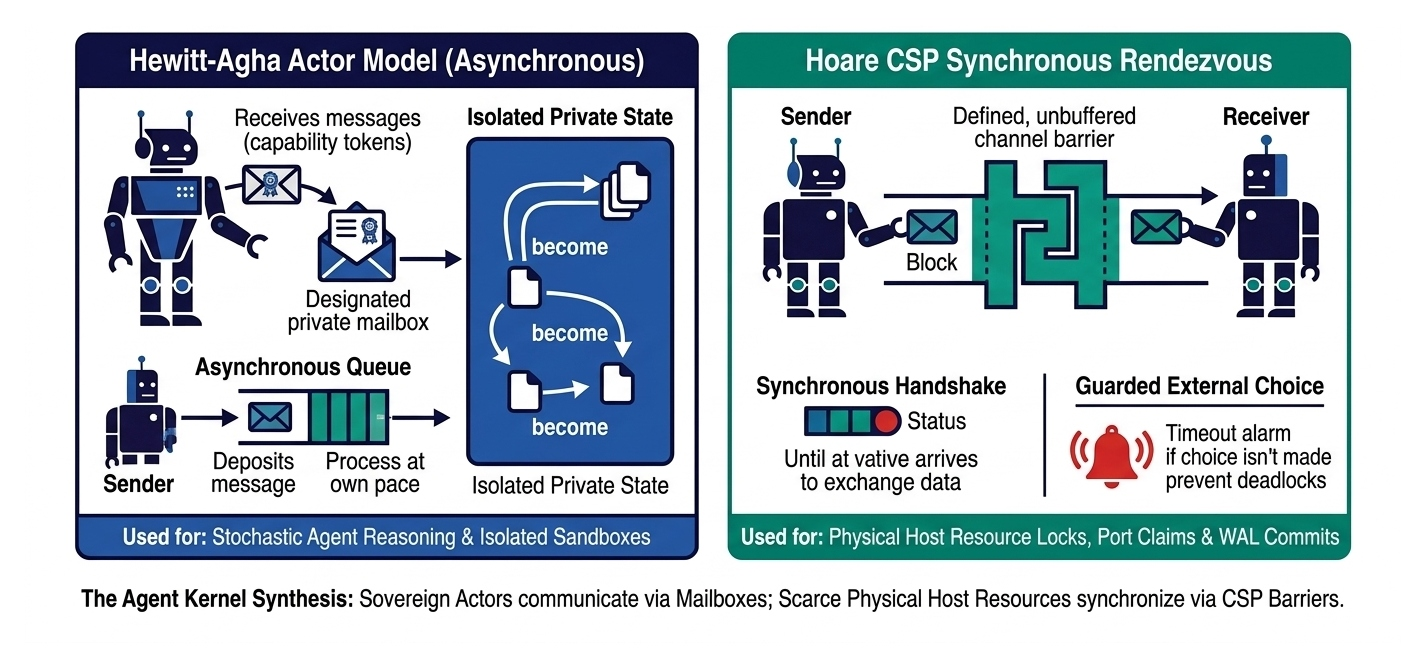
\includegraphics[width=\linewidth,height=8.0cm,keepaspectratio]{figures/fig-ch0-concurrency-diagram.jpg}
    \end{minipage}
    \tcblower
    \begin{minipage}[t][2.0cm][t]{\linewidth}
      \pdgrotesk\scriptsize
      \textbf{\color{pderror!90!black} Artifact \& Limitation Audit:}\\
      \begin{itemize}[leftmargin=9pt,itemsep=0pt,topsep=0.5pt,parsep=0pt]
        \item Asymmetric lifelines with wavy paths and distorted mailbox queues
        \item Rendezvous barrier rendered as a fuzzy blob rather than an instantaneous synchronization
        \item Lack of formal notation for actor replacement behaviors (become)
      \end{itemize}
    \end{minipage}
  \end{tcolorbox}
\end{minipage}\hfill
\begin{minipage}[t]{0.492\linewidth}
  \begin{tcolorbox}[
    colback=pdcobalt!3,colframe=pdcobalt!85!black,arc=1.5pt,
    boxrule=0.7pt,top=1.5pt,bottom=1.5pt,left=4pt,right=4pt,
    title={\pdgrotesk\footnotesize\bfseries \color{white} B. Authoritative Native Vector Replacement \hfill \texttt{.tex / TikZ / PGF}}
  ]
    \begin{minipage}[c][8.3cm][c]{\linewidth}
      \centering
      \sbox{\pdfigbox}{% fig-ch0-concurrency-actors-csp.tex
% Concurrency Foundations: Virtual Actors vs. CSP Rendezvous
% 100% native vector Swiss TikZ spatial replica of the AI-generated diagram prototype.

% pd-robot-glyphs.tex
% Authentic vector robot glyphs and system iconography for Port Daddy architectural figures.
% Provides 100% vector replacements matching the AI-generated diagram prototypes.

\ifdefined\pdrobotglyphsloaded\else
\def\pdrobotglyphsloaded{1}

% -----------------------------------------------------------------------------
% 1. Standard Standing Agent Robot (Base Model)
% Args: shift (x,y), color, scale
% -----------------------------------------------------------------------------
\newcommand{\pdrobotbase}[3][1.0]{%
  \begin{scope}[shift={#2},scale=#1]
    % Head
    \draw[fill=#3!85, draw=#3!95!black, line width=0.6pt, rounded corners=2pt] (-0.28, 0.22) rectangle (0.28, 0.58);
    % Dual Antennae
    \draw[line width=0.65pt, draw=#3!95!black] (-0.12, 0.58) -- (-0.16, 0.72);
    \draw[line width=0.65pt, draw=#3!95!black] (0.12, 0.58) -- (0.16, 0.72);
    \fill[pdamber!90!orange] (-0.16, 0.72) circle (0.038);
    \fill[pdamber!90!orange] (0.16, 0.72) circle (0.038);
    % Screen / Visor
    \draw[fill=hhink!90, draw=none, rounded corners=1.2pt] (-0.22, 0.28) rectangle (0.22, 0.52);
    % Eyes
    \fill[pdteal!35!white] (-0.11, 0.40) circle (0.04);
    \fill[pdteal!35!white] (0.11, 0.40) circle (0.04);
    % Mouth bar
    \draw[pdteal!35!white, line width=0.4pt] (-0.07, 0.33) -- (0.07, 0.33);
    % Ear bolts
    \draw[fill=pdslate!60, draw=#3!95!black, line width=0.4pt] (-0.32, 0.35) rectangle (-0.28, 0.45);
    \draw[fill=pdslate!60, draw=#3!95!black, line width=0.4pt] (0.28, 0.35) rectangle (0.32, 0.45);
    % Neck
    \draw[fill=pdslate!70, draw=#3!95!black, line width=0.4pt] (-0.08, 0.16) rectangle (0.08, 0.22);
    % Body / Torso
    \draw[fill=#3!85, draw=#3!95!black, line width=0.6pt, rounded corners=2pt] (-0.32, -0.28) rectangle (0.32, 0.16);
    % Chest panel
    \draw[fill=pdpage, draw=#3!70!black, line width=0.35pt, rounded corners=1pt] (-0.22, -0.12) rectangle (0.22, 0.10);
    \fill[pdhealth] (-0.13, -0.01) circle (0.03);
    \fill[pdamber] (0.0, -0.01) circle (0.03);
    \fill[pderror] (0.13, -0.01) circle (0.03);
    % Arms
    \draw[fill=#3!75, draw=#3!95!black, line width=0.45pt, rounded corners=1.2pt] (-0.44, -0.20) rectangle (-0.32, 0.10);
    \draw[fill=#3!75, draw=#3!95!black, line width=0.45pt, rounded corners=1.2pt] (0.32, -0.20) rectangle (0.44, 0.10);
    % Legs & Feet
    \draw[fill=pdslate!80, draw=#3!95!black, line width=0.45pt] (-0.24, -0.46) rectangle (-0.09, -0.28);
    \draw[fill=pdslate!80, draw=#3!95!black, line width=0.45pt] (0.09, -0.46) rectangle (0.24, -0.28);
    \draw[fill=pdslate!90!black, draw=#3!95!black, line width=0.45pt, rounded corners=1pt] (-0.28, -0.52) rectangle (-0.05, -0.44);
    \draw[fill=pdslate!90!black, draw=#3!95!black, line width=0.45pt, rounded corners=1pt] (0.05, -0.52) rectangle (0.28, -0.44);
  \end{scope}
}

% -----------------------------------------------------------------------------
% 2. Robot Holding Voting / Lease Token Tablet
% -----------------------------------------------------------------------------
\newcommand{\pdrobottoken}[3][1.0]{%
  \begin{scope}[shift={#2},scale=#1]
    % Head
    \draw[fill=#3!85, draw=#3!95!black, line width=0.6pt, rounded corners=2pt] (-0.28, 0.22) rectangle (0.28, 0.58);
    % Antenna
    \draw[line width=0.65pt, draw=#3!95!black] (0, 0.58) -- (0, 0.73);
    \fill[pdamber!90!orange] (0, 0.73) circle (0.04);
    % Screen / Visor
    \draw[fill=hhink!90, draw=none, rounded corners=1.2pt] (-0.22, 0.28) rectangle (0.22, 0.52);
    \fill[pdteal!35!white] (-0.11, 0.40) circle (0.04);
    \fill[pdteal!35!white] (0.11, 0.40) circle (0.04);
    \draw[pdteal!35!white, line width=0.4pt] (-0.07, 0.33) -- (0.07, 0.33);
    % Neck
    \draw[fill=pdslate!70, draw=#3!95!black, line width=0.4pt] (-0.08, 0.16) rectangle (0.08, 0.22);
    % Body
    \draw[fill=#3!85, draw=#3!95!black, line width=0.6pt, rounded corners=2pt] (-0.32, -0.28) rectangle (0.32, 0.16);
    % Legs & Feet
    \draw[fill=pdslate!80, draw=#3!95!black, line width=0.45pt] (-0.24, -0.46) rectangle (-0.09, -0.28);
    \draw[fill=pdslate!80, draw=#3!95!black, line width=0.45pt] (0.09, -0.46) rectangle (0.24, -0.28);
    \draw[fill=pdslate!90!black, draw=#3!95!black, line width=0.45pt, rounded corners=1pt] (-0.28, -0.52) rectangle (-0.05, -0.44);
    \draw[fill=pdslate!90!black, draw=#3!95!black, line width=0.45pt, rounded corners=1pt] (0.05, -0.52) rectangle (0.28, -0.44);
    % Arms holding tablet
    \draw[fill=#3!75, draw=#3!95!black, line width=0.45pt] (-0.42, -0.08) -- (-0.22, 0.05) -- (-0.18, 0.0) -- (-0.35, -0.13) -- cycle;
    \draw[fill=#3!75, draw=#3!95!black, line width=0.45pt] (0.42, -0.08) -- (0.22, 0.05) -- (0.18, 0.0) -- (0.35, -0.13) -- cycle;
    % Tablet
    \draw[fill=pdpage, draw=pdcobalt, line width=0.55pt, rounded corners=1.2pt] (-0.24, -0.18) rectangle (0.24, 0.18);
    \node[font=\fontsize{3.8}{4.5}\selectfont\bfseries\color{pdcobalt}] at (0, 0.06) {VOTING};
    \node[font=\fontsize{3.5}{4.2}\selectfont\bfseries\color{hhink}] at (0, -0.06) {TOKEN};
  \end{scope}
}

% -----------------------------------------------------------------------------
% 3. Robot at Laptop / Deliberation
% -----------------------------------------------------------------------------
\newcommand{\pdrobotlaptop}[3][1.0]{%
  \begin{scope}[shift={#2},scale=#1]
    % Head (Tilted slightly forward)
    \draw[fill=#3!85, draw=#3!95!black, line width=0.6pt, rounded corners=2pt] (-0.26, 0.22) rectangle (0.26, 0.56);
    % Dual Antennae
    \draw[line width=0.65pt, draw=#3!95!black] (-0.10, 0.56) -- (-0.14, 0.70);
    \draw[line width=0.65pt, draw=#3!95!black] (0.10, 0.56) -- (0.14, 0.70);
    \fill[pdteal] (-0.14, 0.70) circle (0.038);
    \fill[pdteal] (0.14, 0.70) circle (0.038);
    % Visor
    \draw[fill=hhink!90, draw=none, rounded corners=1.2pt] (-0.20, 0.28) rectangle (0.20, 0.50);
    \fill[pdteal!40!white] (-0.10, 0.38) circle (0.038);
    \fill[pdteal!40!white] (0.10, 0.38) circle (0.038);
    % Body
    \draw[fill=#3!85, draw=#3!95!black, line width=0.6pt, rounded corners=2pt] (-0.30, -0.26) rectangle (0.30, 0.18);
    % Legs (Seated)
    \draw[fill=pdslate!80, draw=#3!95!black, line width=0.45pt] (-0.25, -0.38) rectangle (0.25, -0.26);
    % Desk surface
    \draw[line width=1.0pt, pdslate!80!black] (-0.6, -0.38) -- (0.7, -0.38);
    % Laptop Base
    \draw[fill=pdslate!40, draw=pdslate!90!black, line width=0.45pt] (-0.05, -0.38) -- (0.50, -0.38) -- (0.46, -0.33) -- (-0.02, -0.33) -- cycle;
    % Laptop Screen
    \draw[fill=pdcobalt!90!black, draw=pdslate!90!black, line width=0.5pt, rounded corners=1pt] (0.42, -0.33) -- (0.52, 0.05) -- (0.15, 0.05) -- (0.08, -0.33) -- cycle;
    % Glowing Screen Text
    \draw[pdteal!50!white, line width=0.4pt] (0.18, -0.03) -- (0.42, -0.03);
    \draw[pdteal!50!white, line width=0.4pt] (0.16, -0.12) -- (0.38, -0.12);
    \draw[pdteal!50!white, line width=0.4pt] (0.14, -0.21) -- (0.34, -0.21);
    % Arms on keyboard
    \draw[fill=#3!75, draw=#3!95!black, line width=0.45pt] (-0.22, 0.05) to[out=-20,in=160] (0.12, -0.30) -- (0.18, -0.33) -- (-0.18, -0.05) -- cycle;
  \end{scope}
}

% -----------------------------------------------------------------------------
% 4. Red-and-White Disablement Barrier
% -----------------------------------------------------------------------------
\newcommand{\pdbarrierline}[4]{% (x1, y1) to (x2, y2)
  \draw[line width=4.5pt, white] (#1,#2) -- (#3,#4);
  \draw[line width=4.5pt, pderror, dashed, dash pattern=on 6pt off 6pt] (#1,#2) -- (#3,#4);
  \draw[line width=0.6pt, pderror!80!black] (#1,#2) -- (#3,#4);
}

% -----------------------------------------------------------------------------
% 5. Vector Iconography Definitions
% -----------------------------------------------------------------------------
% Crossed Tools (Wrench + Screwdriver)
\newcommand{\pdicontools}[2][1.0]{%
  \begin{scope}[shift={#2},scale=#1]
    \draw[line width=1.4pt, pdslate!80!black, line cap=round] (-0.25,-0.25) -- (0.25,0.25);
    \draw[line width=1.4pt, pdrust!90!black, line cap=round] (-0.25,0.25) -- (0.25,-0.25);
    \draw[fill=pdslate!90!black, line width=0.4pt] (0.18,0.18) circle (0.10);
    \fill[white] (0.20,0.20) circle (0.04);
    \draw[fill=pdrust!90!black, line width=0.4pt] (0.20,-0.22) rectangle (0.26,-0.16);
  \end{scope}
}

% Git Branch
\newcommand{\pdicongit}[2][1.0]{%
  \begin{scope}[shift={#2},scale=#1]
    \draw[line width=1.1pt, pdteal!90!black] (0,-0.32) -- (0,0.32);
    \draw[line width=1.1pt, pdteal!90!black] (0,-0.08) to[out=45,in=180] (0.24,0.16);
    \fill[pdteal!90!black] (0,-0.24) circle (0.06);
    \fill[pdteal!90!black] (0,0.24) circle (0.06);
    \fill[pdteal!90!black] (0.24,0.16) circle (0.06);
  \end{scope}
}

% Network Globe
\newcommand{\pdiconglobe}[2][1.0]{%
  \begin{scope}[shift={#2},scale=#1]
    \draw[line width=0.7pt, pdcobalt!85!black] (0,0) circle (0.28);
    \draw[line width=0.5pt, pdcobalt!70] (0,0) ellipse (0.13 and 0.28);
    \draw[line width=0.5pt, pdcobalt!70] (-0.28,0) -- (0.28,0);
    \draw[line width=0.5pt, pdcobalt!70] (-0.24,0.14) -- (0.24,0.14);
    \draw[line width=0.5pt, pdcobalt!70] (-0.24,-0.14) -- (0.24,-0.14);
  \end{scope}
}

% Host OS Gear / Process
\newcommand{\pdicongear}[2][1.0]{%
  \begin{scope}[shift={#2},scale=#1]
    \fill[pdslate!75!black] (0,0) circle (0.22);
    \foreach \a in {0,45,90,135,180,225,270,315} {
      \fill[pdslate!75!black] (\a:0.26) circle (0.055);
    }
    \fill[white] (0,0) circle (0.09);
  \end{scope}
}

% Stopwatch / Timer
\newcommand{\pdicontimer}[2][1.0]{%
  \begin{scope}[shift={#2},scale=#1]
    \draw[line width=0.75pt, pdamber!90!black] (0,0) circle (0.25);
    \draw[line width=0.8pt, pdamber!90!black] (0,0.25) -- (0,0.33);
    \draw[line width=1.0pt, pdamber!90!black] (-0.06,0.33) -- (0.06,0.33);
    \draw[line width=0.75pt, pdamber!90!black] (0,0) -- (0,0.14);
    \draw[line width=0.75pt, pdamber!90!black] (0,0) -- (0.11,0.05);
    \fill[pdamber!90!black] (0,0) circle (0.035);
  \end{scope}
}

% Hardware Crash / Lightning Burst
\newcommand{\pdiconcrash}[2][1.0]{%
  \begin{scope}[shift={#2},scale=#1]
    \fill[pderror!90!black] (0.06,0.32) -- (-0.12,0.04) -- (-0.02,0.04) -- (-0.14,-0.32) -- (0.12,-0.02) -- (0.02,-0.02) -- cycle;
  \end{scope}
}

% Shield with Checkmark
\newcommand{\pdiconshieldcheck}[2][1.0]{%
  \begin{scope}[shift={#2},scale=#1]
    \fill[pdcobalt!90!black] (0,0.32) -- (0.26,0.20) to[out=-70,in=45] (0,-0.32) to[out=135,in=-110] (-0.26,0.20) -- cycle;
    \draw[line width=1.1pt, white, line cap=round, line join=round] (-0.11,-0.02) -- (-0.03,-0.12) -- (0.13,0.10);
  \end{scope}
}

% Padlock
\newcommand{\pdiconlock}[2][1.0]{%
  \begin{scope}[shift={#2},scale=#1]
    % Shackle
    \draw[line width=0.9pt, pdslate!80!black] (-0.12,0.05) -- (-0.12,0.18) arc (180:0:0.12) -- (0.12,0.05);
    % Body
    \draw[fill=pderror!85!black, draw=pderror!95!black, line width=0.5pt, rounded corners=1pt] (-0.18,-0.20) rectangle (0.18,0.06);
    % Keyhole
    \fill[white] (0,-0.04) circle (0.035);
    \draw[line width=0.6pt, white] (0,-0.04) -- (0,-0.13);
  \end{scope}
}

% Speedometer / Spend Cap
\newcommand{\pdiconspeedometer}[2][1.0]{%
  \begin{scope}[shift={#2},scale=#1]
    \draw[line width=1.0pt, pdteal!90!black] (-0.28,-0.04) arc (180:40:0.28);
    \draw[line width=1.0pt, pderror] (40:0.28) arc (40:0:0.28);
    \draw[line width=0.8pt, hhink, line cap=round] (0,-0.04) -- (0.12,0.14);
    \fill[hhink] (0,-0.04) circle (0.05);
  \end{scope}
}

% Sparkle Broom / Hygiene Wand
\newcommand{\pdiconbroom}[2][1.0]{%
  \begin{scope}[shift={#2},scale=#1]
    \draw[line width=1.2pt, pdteal!90!black, line cap=round] (-0.2,-0.2) -- (0.15,0.15);
    % Sparkles
    \fill[pdamber!90!orange] (0.22,0.22) circle (0.04);
    \fill[pdteal] (0.05,0.26) circle (0.03);
    \fill[pdteal] (0.26,0.05) circle (0.03);
  \end{scope}
}

% Host Terminal Substrate
\newcommand{\pdiconterminal}[2][1.0]{%
  \begin{scope}[shift={#2},scale=#1]
    \draw[fill=hhink!95, draw=pdslate!80, line width=0.6pt, rounded corners=1.5pt] (-0.35,-0.25) rectangle (0.35,0.25);
    \draw[fill=pderror] (-0.26,0.18) circle (0.025);
    \fill[pdamber] (-0.18,0.18) circle (0.025);
    \fill[pdhealth] (-0.10,0.18) circle (0.025);
    \node[font=\fontsize{4.5}{5}\selectfont\ttfamily\color{pdhealth}] at (0,-0.05) {>\_};
  \end{scope}
}

% Coins Stack
\newcommand{\pdiconcoins}[2][1.0]{%
  \begin{scope}[shift={#2},scale=#1]
    \foreach \y in {-0.24, -0.12, 0.0, 0.12} {
      \draw[fill=pdamber!80!orange, draw=pdamber!95!black, line width=0.45pt] (0,\y) ellipse (0.24 and 0.07);
    }
  \end{scope}
}

% Tall Coins Stack
\newcommand{\pdiconcoinstall}[2][1.0]{%
  \begin{scope}[shift={#2},scale=#1]
    \foreach \y in {-0.30, -0.18, -0.06, 0.06, 0.18, 0.30} {
      \draw[fill=pdamber!80!orange, draw=pdamber!95!black, line width=0.45pt] (0,\y) ellipse (0.24 and 0.07);
    }
  \end{scope}
}

% Slashed Coins (Stake Slashed)
\newcommand{\pdiconcoinslashed}[2][1.0]{%
  \begin{scope}[shift={#2},scale=#1]
    \foreach \y in {-0.20, -0.08, 0.04, 0.16} {
      \draw[fill=pdamber!70!white, draw=pdamber!80!black, line width=0.45pt] (0,\y) ellipse (0.22 and 0.065);
    }
    \draw[line width=1.5pt, pderror, line cap=round] (-0.26,-0.24) -- (0.26,0.24);
  \end{scope}
}

% Magnifying Glass (Audit Inspection)
\newcommand{\pdiconmagnifier}[2][1.0]{%
  \begin{scope}[shift={#2},scale=#1]
    \draw[line width=0.9pt, pdteal!90!black] (0,0.06) circle (0.16);
    \draw[line width=1.4pt, pdteal!90!black, line cap=round] (0.12,-0.06) -- (0.26,-0.20);
    \fill[white] (-0.04,0.10) circle (0.04);
  \end{scope}
}

% Arbitration Gavel & Scales of Justice
\newcommand{\pdiconarbitration}[2][1.0]{%
  \begin{scope}[shift={#2},scale=#1]
    % Central post
    \draw[line width=0.8pt, pdrust!90!black] (0.15,-0.20) -- (0.15,0.22);
    \draw[line width=0.8pt, pdrust!90!black] (-0.05,0.18) -- (0.35,0.18);
    \draw[line width=0.5pt, pdrust!80] (-0.05,0.18) -- (-0.12,0.02) -- (0.02,0.02) -- cycle;
    \draw[line width=0.5pt, pdrust!80] (0.35,0.18) -- (0.28,0.02) -- (0.42,0.02) -- cycle;
    % Gavel
    \draw[line width=1.4pt, pdrust!95!black, line cap=round] (-0.30,-0.18) -- (-0.10,0.05);
    \draw[fill=pdrust!90!black, draw=pdrust!95!black, line width=0.5pt, rounded corners=1pt] (-0.22,0.0) -- (-0.12,0.12) -- (-0.02,0.04) -- (-0.12,-0.08) -- cycle;
  \end{scope}
}

% Cash Bill / Liquidated Damages
\newcommand{\pdiconcash}[2][1.0]{%
  \begin{scope}[shift={#2},scale=#1]
    \draw[fill=white, draw=pdslate!90!black, line width=0.6pt, rounded corners=1.5pt] (-0.35,-0.20) rectangle (0.35,0.20);
    \draw[line width=0.5pt, pdteal!80!black] (-0.28,-0.14) rectangle (0.28,0.14);
    \fill[pdteal!90!black] (0,0) circle (0.08);
    \fill[pdteal!90!black] (-0.22,0) circle (0.035);
    \fill[pdteal!90!black] (0.22,0) circle (0.035);
  \end{scope}
}

% Group of People / Remedy
\newcommand{\pdicongrouppeople}[2][1.0]{%
  \begin{scope}[shift={#2},scale=#1]
    % Center person
    \fill[hhink] (0,0.12) circle (0.09);
    \fill[hhink] (-0.15,-0.20) to[out=70,in=180] (0,-0.02) to[out=0,in=110] (0.15,-0.20) -- cycle;
    % Left person
    \fill[hhgray!90!black] (-0.22,0.06) circle (0.075);
    \fill[hhgray!90!black] (-0.34,-0.20) to[out=70,in=180] (-0.22,-0.06) to[out=0,in=110] (-0.10,-0.20) -- cycle;
    % Right person
    \fill[hhgray!90!black] (0.22,0.06) circle (0.075);
    \fill[hhgray!90!black] (0.10,-0.20) to[out=70,in=180] (0.22,-0.06) to[out=0,in=110] (0.34,-0.20) -- cycle;
  \end{scope}
}

% Database Cylinder
\newcommand{\pdicondatabase}[2][1.0]{%
  \begin{scope}[shift={#2},scale=#1]
    \draw[fill=pdslate!20, draw=pdslate!90!black, line width=0.6pt] (-0.25,-0.15) rectangle (0.25,0.15);
    \draw[fill=pdslate!30, draw=pdslate!90!black, line width=0.5pt] (0,0.15) ellipse (0.25 and 0.08);
    \draw[draw=pdslate!90!black, line width=0.5pt] (-0.25,0) arc (180:360:0.25 and 0.08);
    \draw[draw=pdslate!90!black, line width=0.5pt] (-0.25,-0.15) arc (180:360:0.25 and 0.08);
  \end{scope}
}

% Signed Document / Witness Receipts
\newcommand{\pdicondocument}[2][1.0]{%
  \begin{scope}[shift={#2},scale=#1]
    \draw[fill=white, draw=pdslate!90!black, line width=0.55pt] (-0.18,-0.24) -- (0.10,-0.24) -- (0.18,-0.16) -- (0.18,0.24) -- (-0.18,0.24) -- cycle;
    \draw[draw=pdslate!80, line width=0.45pt] (0.10,-0.24) -- (0.10,-0.16) -- (0.18,-0.16);
    \draw[pdslate!70, line width=0.4pt] (-0.12,0.16) -- (0.12,0.16);
    \draw[pdslate!70, line width=0.4pt] (-0.12,0.08) -- (0.12,0.08);
    \draw[pdslate!70, line width=0.4pt] (-0.12,0.00) -- (0.06,0.00);
    % Feather / quill
    \draw[line width=0.7pt, pdcobalt!80!black] (0.08,-0.12) to[out=45,in=-45] (0.24,0.06);
  \end{scope}
}

% Merkle Inclusion Proof Tree
\newcommand{\pdiconmerkle}[2][1.0]{%
  \begin{scope}[shift={#2},scale=#1]
    % Root
    \draw[line width=0.5pt, pdslate!80] (0,0.20) -- (-0.16,0.04);
    \draw[line width=0.5pt, pdslate!80] (0,0.20) -- (0.16,0.04);
    \draw[line width=0.5pt, pdslate!80] (-0.16,0.04) -- (-0.24,-0.14);
    \draw[line width=0.5pt, pdslate!80] (-0.16,0.04) -- (-0.08,-0.14);
    \draw[line width=0.5pt, pdslate!80] (0.16,0.04) -- (0.08,-0.14);
    \draw[line width=0.5pt, pdslate!80] (0.16,0.04) -- (0.24,-0.14);
    \draw[fill=white, draw=pdslate!90!black, line width=0.4pt] (-0.05,0.16) rectangle (0.05,0.24);
    \draw[fill=white, draw=pdslate!90!black, line width=0.4pt] (-0.20,0.0) rectangle (-0.12,0.08);
    \draw[fill=white, draw=pdslate!90!black, line width=0.4pt] (0.12,0.0) rectangle (0.20,0.08);
    \draw[fill=pdteal!80!white, draw=pdteal!95!black, line width=0.5pt] (-0.28,-0.18) rectangle (-0.20,-0.10);
    \draw[fill=white, draw=pdslate!90!black, line width=0.4pt] (-0.12,-0.18) rectangle (-0.04,-0.10);
    \draw[fill=white, draw=pdslate!90!black, line width=0.4pt] (0.04,-0.18) rectangle (0.12,-0.10);
    \draw[fill=white, draw=pdslate!90!black, line width=0.4pt] (0.20,-0.18) rectangle (0.28,-0.10);
  \end{scope}
}

% Key (Cryptographic Key / Capability Key)
\newcommand{\pdiconkey}[2][1.0]{%
  \begin{scope}[shift={#2},scale=#1]
    \draw[line width=0.8pt, pdamber!95!black] (0, 0.12) circle (0.14);
    \fill[white] (0, 0.12) circle (0.06);
    \draw[line width=0.85pt, pdamber!95!black] (0, -0.02) -- (0, -0.26);
    \draw[line width=0.7pt, pdamber!95!black] (0, -0.14) -- (0.10, -0.14);
    \draw[line width=0.7pt, pdamber!95!black] (0, -0.22) -- (0.08, -0.22);
  \end{scope}
}

\def\pdiconclock{\pdicontimer}
\def\pdiconlightning{\pdiconcrash}

\fi

\pdfigurehue{pdcobalt}%
\begin{tikzpicture}[pd figure,x=1cm,y=1cm]
  \tikzset{
    containerbox/.style={draw=pdslate!40,line width=0.7pt,fill=white,rounded corners=3.5pt},
    headerpill/.style={line width=0pt,rounded corners=2.5pt},
    usedforpill/.style={draw=none,fill=pdcobalt!90!black,rounded corners=2pt,inner xsep=6pt,inner ysep=2.5pt},
    cardbox/.style={draw=pdslate!30,line width=0.5pt,fill=hhpaper!30,rounded corners=2pt,inner sep=2pt}
  }

  % =========================================================================
  % LEFT PANEL: HEWITT-AGHA ACTOR MODEL (x in [0.1, 6.6])
  % =========================================================================
  \draw[containerbox] (0.1, 0.65) rectangle (6.6, 5.15);
  % Header (Navy)
  \draw[fill=pdcobalt!90!black,draw=none,rounded corners=2.5pt] (0.14, 4.75) rectangle (6.56, 5.11);
  \node[font=\fontsize{5.6}{6.8}\selectfont\bfseries\color{white}] at (3.35, 4.93) {%
    Hewitt-Agha Actor Model (Asynchronous)%
  };

  % Robot Receiver (Left)
  \pdrobotbase[0.65]{(0.9, 3.8)}{pdcobalt}
  \node[font=\fontsize{4.6}{5.4}\selectfont\color{hhink},align=center] at (2.2, 4.35) {%
    Receives messages\\{\fontsize{4.0}{4.8}\selectfont(capability tokens)}%
  };

  % Envelope with token
  \begin{scope}[shift={(1.85, 3.8)}]
    \draw[fill=white,draw=pdcobalt,line width=0.5pt,rounded corners=1pt] (-0.35, -0.22) rectangle (0.35, 0.22);
    \draw[line width=0.4pt,pdcobalt] (-0.35, 0.22) -- (0, -0.05) -- (0.35, 0.22);
    \draw[pd arrow,line width=0.6pt,pdcobalt] (0.45, 0) -- (0.85, 0);
  \end{scope}

  % Designated private mailbox
  \begin{scope}[shift={(2.5, 3.1)}]
    \draw[cardbox] (-1.0, -0.4) rectangle (1.0, 0.4);
    \node[font=\fontsize{4.6}{5.5}\selectfont\bfseries\color{hhink},align=center] at (0, 0.15) {%
      Designated\\private mailbox%
    };
    % mini queue bar
    \draw[fill=pdteal!30,draw=pdteal,line width=0.4pt,rounded corners=1pt] (-0.7, -0.3) rectangle (0.7, -0.08);
    \draw[pdteal,line width=0.4pt] (-0.25, -0.3) -- (-0.25, -0.08);
    \draw[pdteal,line width=0.4pt] (0.25, -0.3) -- (0.25, -0.08);
  \end{scope}

  % Isolated Private State (Right Column of Actor Panel)
  \begin{scope}[shift={(5.1, 3.3)}]
    \draw[draw=pdslate!40,line width=0.6pt,fill=hhpaper!15,rounded corners=2.5pt] (-1.25, -1.8) rectangle (1.25, 0.85);
    \node[font=\fontsize{4.8}{5.8}\selectfont\bfseries\color{pdcobalt}] at (0, 0.65) {Isolated Private State};
    % 3 Become pills
    \draw[fill=pdcobalt!85,draw=none,rounded corners=2pt] (-0.95, 0.15) rectangle (0.95, 0.48);
    \node[font=\fontsize{4.6}{5.5}\selectfont\bfseries\color{white}] at (0, 0.315) {become};

    \draw[fill=pdcobalt!85,draw=none,rounded corners=2pt] (-0.95, -0.35) rectangle (0.95, -0.02);
    \node[font=\fontsize{4.6}{5.5}\selectfont\bfseries\color{white}] at (0, -0.185) {become};

    \draw[fill=pdcobalt!85,draw=none,rounded corners=2pt] (-0.95, -0.85) rectangle (0.95, -0.52);
    \node[font=\fontsize{4.6}{5.5}\selectfont\bfseries\color{white}] at (0, -0.685) {become};

    \draw[pd arrow,line width=0.6pt,pdcobalt] (0, 0.15) -- (0, -0.02);
    \draw[pd arrow,line width=0.6pt,pdcobalt] (0, -0.35) -- (0, -0.52);
  \end{scope}

  % Asynchronous Queue label & arrow
  \node[font=\fontsize{4.6}{5.5}\selectfont\bfseries\color{hhink}] at (2.5, 2.35) {Asynchronous Queue};
  \draw[pd arrow,line width=0.8pt,pdcobalt] (1.3, 2.0) -- (3.7, 2.0);
  \node[font=\fontsize{4.2}{5.0}\selectfont\color{hhgray!90!black},align=center] at (1.5, 1.7) {Deposits\\message};
  \node[font=\fontsize{4.2}{5.0}\selectfont\color{hhgray!90!black},align=center] at (3.5, 1.7) {Process at\\own pace};

  % Bottom Pill: Used for
  \node[usedforpill,anchor=south] at (3.35, 0.72) {%
    {\fontsize{4.5}{5.4}\selectfont\color{white}\textbf{Used for:} Stochastic Agent Reasoning \& Isolated Sandboxes}%
  };

  % =========================================================================
  % RIGHT PANEL: HOARE CSP SYNCHRONOUS RENDEZVOUS (x in [6.9, 13.5])
  % =========================================================================
  \draw[containerbox] (6.9, 0.65) rectangle (13.5, 5.15);
  % Header (Teal)
  \draw[fill=pdteal!90!black,draw=none,rounded corners=2.5pt] (6.94, 4.75) rectangle (13.46, 5.11);
  \node[font=\fontsize{5.6}{6.8}\selectfont\bfseries\color{white}] at (10.2, 4.93) {%
    Hoare CSP Synchronous Rendezvous%
  };

  % Sender Robot (Left)
  \pdrobotbase[0.62]{(7.6, 3.8)}{pdteal}
  \node[font=\fontsize{4.6}{5.4}\selectfont\bfseries\color{hhink}] at (7.6, 4.45) {Sender};

  % Receiver Robot (Right)
  \pdrobotbase[0.62]{(12.8, 3.8)}{pdcobalt}
  \node[font=\fontsize{4.6}{5.4}\selectfont\bfseries\color{hhink}] at (12.8, 4.45) {Receiver};

  % Defined, unbuffered channel barrier (Interlocking Gate in Center)
  \begin{scope}[shift={(10.2, 3.8)}]
    \node[font=\fontsize{4.5}{5.4}\selectfont\bfseries\color{hhink},align=center] at (0, 0.65) {%
      Defined, unbuffered\\channel barrier%
    };
    % Interlocking Gate / Barrier
    \draw[fill=pdteal!30,draw=pdteal!90!black,line width=0.6pt] (-0.8, -0.3) rectangle (-0.2, 0.3);
    \draw[fill=pdcobalt!30,draw=pdcobalt!90!black,line width=0.6pt] (0.2, -0.3) rectangle (0.8, 0.3);
    \draw[fill=white,draw=pderror,line width=0.7pt,rounded corners=1pt] (-0.3, -0.15) rectangle (0.3, 0.15);
    \node[font=\fontsize{4.2}{5.0}\selectfont\bfseries\color{pderror}] at (0, 0) {Block};
  \end{scope}

  % Synchronous Handshake Card (Left Bottom of CSP)
  \begin{scope}[shift={(8.45, 2.25)}]
    \draw[cardbox] (-1.25, -0.7) rectangle (1.25, 0.55);
    \node[font=\fontsize{4.6}{5.5}\selectfont\bfseries\color{hhink}] at (0, 0.38) {Synchronous Handshake};
    % Status bar
    \draw[fill=pdhealth,draw=none] (-0.6, 0.12) rectangle (-0.3, 0.24);
    \draw[fill=pdhealth,draw=none] (-0.2, 0.12) rectangle (0.1, 0.24);
    \draw[fill=pdhealth,draw=none] (0.2, 0.12) rectangle (0.5, 0.24);
    \node[font=\fontsize{4.0}{4.8}\selectfont\bfseries\color{pdhealth!90!black}] at (0.8, 0.18) {Status};
    \node[font=\fontsize{4.2}{5.0}\selectfont\color{hhgray!90!black},align=center,text width=2.3cm] at (0, -0.28) {%
      Until at valive arrives\\to exchange data%
    };
  \end{scope}

  % Guarded External Choice Card (Right Bottom of CSP)
  \begin{scope}[shift={(11.95, 2.25)}]
    \draw[cardbox] (-1.25, -0.7) rectangle (1.25, 0.55);
    \node[font=\fontsize{4.6}{5.5}\selectfont\bfseries\color{hhink}] at (0, 0.38) {Guarded External Choice};
    % Bell / Alarm icon
    \pdiconcrash[0.45]{(-0.8, -0.05)}
    \node[font=\fontsize{4.2}{5.0}\selectfont\color{hhgray!90!black},align=left,text width=1.6cm] at (0.25, -0.1) {%
      Timeout alarm\\if choice isn't made\\prevent deadlocks%
    };
  \end{scope}

  % Bottom Pill: Used for
  \node[usedforpill,anchor=south] at (10.2, 0.72) {%
    {\fontsize{4.5}{5.4}\selectfont\color{white}\textbf{Used for:} Physical Host Resource Locks, Port Claims \& WAL Commits}%
  };

  % =========================================================================
  % BOTTOM FOOTER BANNER (x in [0.1, 13.5])
  % =========================================================================
  \node[draw=pdcobalt!40,line width=0.5pt,fill=pdcobalt!5,rounded corners=2pt,anchor=south,inner xsep=6pt,inner ysep=2.5pt] at (6.8, 0.1) {%
    {\fontsize{4.8}{5.8}\selectfont\color{hhink}\textbf{The Agent Kernel Synthesis:} Sovereign Actors communicate via Mailboxes; Scarce Physical Host Resources synchronize via CSP Barriers.}%
  };

\end{tikzpicture}
}
      \pdautoscale{8.0cm}{\linewidth}
    \end{minipage}
    \tcblower
    \begin{minipage}[t][2.0cm][t]{\linewidth}
      \pdgrotesk\scriptsize
      \textbf{{\color{pdcobalt} Engineering \& Typography Guarantees:}}\\
      \begin{itemize}[leftmargin=9pt,itemsep=0pt,topsep=0.5pt,parsep=0pt]
        \item Side-by-side comparison of asynchronous Actor mailboxes vs. synchronous CSP rendezvous
        \item Explicit zero-duration synchronization barrier ($\Delta t = 0$) with lease timeout guards
        \item Formal state transitions: $\mathtt{become}(B')$, unbuffered channels, and external choice
      \end{itemize}
    \end{minipage}
  \end{tcolorbox}
\end{minipage}

\vspace*{0.05cm}
\noindent
\begin{tcolorbox}[
  colback=hhpaper,colframe=hhgray!35,arc=1.5pt,boxrule=0.4pt,
  top=1.5pt,bottom=1.5pt,left=6pt,right=6pt
]
  \pdgrotesk\scriptsize
  \noindent
  \textbf{Visual Substrate:} Lossy Bitmap Raster $\rightarrow$ \textbf{\color{pdcobalt}Native PDF / PostScript Vector}\hfill
  \textbf{Text Engine:} Pixelated Approximations $\rightarrow$ \textbf{\color{pdcobalt}Book Typography (OpenType)}\hfill
  \textbf{Resolution:} Fixed DPI Limit $\rightarrow$ \textbf{\color{pdcobalt}Infinite Resolution ($\infty$)}\hfill
  \textbf{Status:} \textbf{\color{pdteal}RECONCILED \& VERIFIED}
\end{tcolorbox}
\clearpage

% =========================================================================
% PAGE 11: Figure 0.11
% =========================================================================
\noindent
\begin{minipage}[t]{\linewidth}
  \noindent{\pdgrotesk\large\bfseries Figure 0.11 \textperiodcentered\ FIPA-00037 Communicative Speech Act State Machine}\hfill
  {\pdgrotesk\footnotesize\color{hhgray} Section 0.1.5 · Agent Communication Languages · Speech Acts \& Performatives}\\
  \vspace*{0.03cm}
  \noindent{\color{hhgray!40}\rule{\linewidth}{0.5pt}}
\end{minipage}

\vspace*{0.05cm}
\noindent
\begin{minipage}[t]{0.492\linewidth}
  \begin{tcolorbox}[
    colback=pdslate!4,colframe=pdslate!70!black,arc=1.5pt,
    boxrule=0.6pt,top=1.5pt,bottom=1.5pt,left=4pt,right=4pt,
    title={\pdgrotesk\footnotesize\bfseries \color{white} A. AI-Generated Raster Prototype (Diffusion / Nano Banana) \hfill \texttt{.jpg / .png}}
  ]
    \begin{minipage}[c][8.3cm][c]{\linewidth}
      \centering
      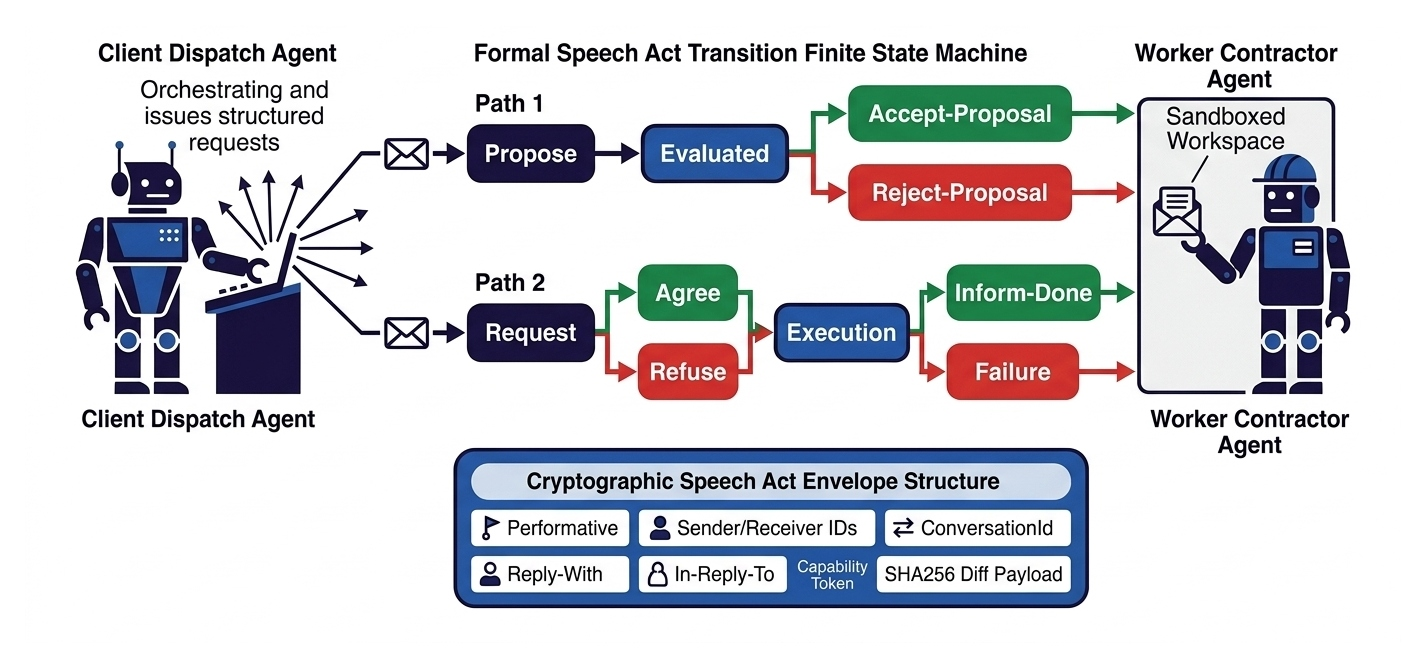
\includegraphics[width=\linewidth,height=8.0cm,keepaspectratio]{figures/fig-ch0-fipa-speech-acts.jpg}
    \end{minipage}
    \tcblower
    \begin{minipage}[t][2.0cm][t]{\linewidth}
      \pdgrotesk\scriptsize
      \textbf{\color{pderror!90!black} Artifact \& Limitation Audit:}\\
      \begin{itemize}[leftmargin=9pt,itemsep=0pt,topsep=0.5pt,parsep=0pt]
        \item Speech bubble shapes look like comic illustrations rather than formal protocols
        \item Performative labels (inform, request, propose) are blurry and unsearchable
        \item Protocol branching logic is incomplete and missing error return paths
      \end{itemize}
    \end{minipage}
  \end{tcolorbox}
\end{minipage}\hfill
\begin{minipage}[t]{0.492\linewidth}
  \begin{tcolorbox}[
    colback=pdcobalt!3,colframe=pdcobalt!85!black,arc=1.5pt,
    boxrule=0.7pt,top=1.5pt,bottom=1.5pt,left=4pt,right=4pt,
    title={\pdgrotesk\footnotesize\bfseries \color{white} B. Authoritative Native Vector Replacement \hfill \texttt{.tex / TikZ / PGF}}
  ]
    \begin{minipage}[c][8.3cm][c]{\linewidth}
      \centering
      \sbox{\pdfigbox}{% fig-ch0-fipa-speech-acts.tex
% FIPA-00037 Communicative Speech Act State Transition Machine
% Replaces raster fig-ch0-fipa-speech-acts.jpg with 100% native vector Swiss TikZ.
\pdfigurehue{pdindigo}%
\begin{tikzpicture}[pd figure,x=1cm,y=1cm]
  \tikzset{
    actnode/.style={draw=hhink,line width=0.7pt,fill=pdpage,rounded corners=2pt,align=center,font=\footnotesize,inner xsep=4pt,inner ysep=3pt},
    stateinit/.style={draw=pdindigo,line width=1.0pt,fill=pdindigo!8,rounded corners=3pt,align=center,font=\footnotesize,inner xsep=5pt,inner ysep=4pt},
    staterun/.style={draw=pdcobalt,line width=0.9pt,fill=pdcobalt!8,rounded corners=3pt,align=center,font=\footnotesize,inner xsep=5pt,inner ysep=4pt},
    statedone/.style={draw=pdhealth,line width=1.1pt,fill=pdhealth!10,rounded corners=3pt,align=center,font=\footnotesize,inner xsep=5pt,inner ysep=4pt},
    statefail/.style={draw=pderror,line width=0.9pt,dashed,fill=pderror!8,rounded corners=3pt,align=center,font=\footnotesize,inner xsep=5pt,inner ysep=4pt},
    panel/.style={draw=hhink!20,line width=0.5pt,densely dotted,rounded corners=3pt,fill=hhpaper!30}
  }

  % Three horizontal pipeline panels (height 3.2 each, 0.3 gap, total height 10.2)
  % =========================================================================
  % 1. DIRECTIVE PIPELINE: request (DB Migration under lock)
  % =========================================================================
  \draw[panel] (0.0,7.0) rectangle (15.2,10.2);
  \node[anchor=north west,font=\pdfiglabelsize\bfseries,text=pdindigo] at (0.2,9.95) {1. DIRECTIVE: \texttt{request} \normalfont\footnotesize\color{hhgray}(Atomic Action Execution)};
  \node[anchor=north east,font=\tiny\sffamily,text=hhgray] at (15.0,9.95) {$\langle\mathtt{conv\_id}, \mathtt{sender}, \mathtt{token}, \mathtt{action}\rangle$};

  % Row 1: Active Lifecycle (y = 8.8)
  \node[stateinit] (req_init) at (1.8,8.8) {%
    \textbf{Initiated}\\
    \scriptsize \texttt{request(db:migrate)}
  };

  \node[actnode,text width=2.6cm] (req_eval) at (5.4,8.8) {%
    \textbf{Arbitration}\\
    \scriptsize Lock \& capability
  };

  \node[staterun] (req_exec) at (9.6,8.8) {%
    \textbf{Agreed \& Sandboxed}\\
    \scriptsize \texttt{agree} $\to$ run migration
  };

  \node[statedone] (req_done) at (13.6,8.8) {%
    \textbf{Completed}\\
    \scriptsize \texttt{inform-done(receipt)}
  };

  % Row 2: Terminal Failure / Refusal (y = 7.55)
  \node[statefail,text width=2.8cm] (req_refuse) at (5.4,7.55) {%
    \textbf{Refused}\\
    \scriptsize \texttt{refuse(lock:held)}
  };

  \node[statefail,text width=2.8cm] (req_fail) at (9.6,7.55) {%
    \textbf{Failed}\\
    \scriptsize \texttt{failure(stderr)}
  };

  % Directive Arrows
  \draw[pd arrow,pdindigo] (req_init.east) -- (req_eval.west);
  \draw[pd arrow,pdcobalt] (req_eval.east) -- (req_exec.west);
  \draw[pd ready arrow] (req_exec.east) -- (req_done.west);
  \draw[pd breach arrow] (req_eval.south) -- (req_refuse.north);
  \draw[pd breach arrow] (req_exec.south) -- (req_fail.north);


  % =========================================================================
  % 2. ASSERTIVE PIPELINE: inform (Belief Base Mutation)
  % =========================================================================
  \draw[panel] (0.0,3.5) rectangle (15.2,6.7);
  \node[anchor=north west,font=\pdfiglabelsize\bfseries,text=pdteal] at (0.2,6.45) {2. ASSERTIVE: \texttt{inform} \normalfont\footnotesize\color{hhgray}(Belief Base Mutation)};
  \node[anchor=north east,font=\tiny\sffamily,text=hhgray] at (15.0,6.45) {Truth commitment: $\operatorname{Bel}_s(p) \land \operatorname{Des}_s(\operatorname{Bel}_r(p))$};

  % Row 1: Active Lifecycle (y = 5.3)
  \node[stateinit,draw=pdteal,fill=pdteal!8] (inf_init) at (1.8,5.3) {%
    \textbf{Asserted}\\
    \scriptsize \texttt{inform(status:green)}
  };

  \node[actnode,text width=2.6cm] (inf_verify) at (5.4,5.3) {%
    \textbf{Integrity Check}\\
    \scriptsize Ed25519 signature
  };

  \node[statedone] (inf_commit) at (13.6,5.3) {%
    \textbf{Belief Mutated}\\
    \scriptsize $+b \in bs$ committed to WAL
  };

  % Row 2: Malformed / Rejected (y = 4.05)
  \node[statefail,text width=3.4cm] (inf_rej) at (5.4,4.05) {%
    \textbf{Not Understood}\\
    \scriptsize \texttt{not-understood(bad:sig)}
  };

  % Assertive Arrows
  \draw[pd arrow,pdteal] (inf_init.east) -- (inf_verify.west);
  \draw[pd ready arrow] (inf_verify.east) -- node[above,font=\tiny,text=pdhealth] {valid cryptographic proof $\to$ commit} (inf_commit.west);
  \draw[pd breach arrow] (inf_verify.south) -- (inf_rej.north);


  % =========================================================================
  % 3. COMMISSIVE PIPELINE: propose (Contract / SLA Negotiation)
  % =========================================================================
  \draw[panel] (0.0,0.0) rectangle (15.2,3.2);
  \node[anchor=north west,font=\pdfiglabelsize\bfseries,text=pdgold] at (0.2,2.95) {3. COMMISSIVE: \texttt{propose} \normalfont\footnotesize\color{hhgray}(SLA \& Work Allocation)};
  \node[anchor=north east,font=\tiny\sffamily,text=hhgray] at (15.0,2.95) {Mutual covenant: $\operatorname{Int}_s(\alpha) \land \operatorname{Commit}(s, r, \alpha)$};

  % Row 1: Active Lifecycle (y = 1.8)
  \node[stateinit,draw=pdgold,fill=pdgold!10] (prop_init) at (1.8,1.8) {%
    \textbf{Proposed}\\
    \scriptsize \texttt{propose(sla:99.9\%)}
  };

  \node[actnode,text width=2.6cm] (prop_eval) at (5.4,1.8) {%
    \textbf{Utility Filter}\\
    \scriptsize Capacity \& budget
  };

  \node[staterun,draw=pdgold,fill=pdgold!8] (prop_acc) at (9.6,1.8) {%
    \textbf{Accepted}\\
    \scriptsize \texttt{accept-proposal}
  };

  \node[statedone] (prop_bound) at (13.6,1.8) {%
    \textbf{Escrow Bound}\\
    \scriptsize Bidirectional lease locked
  };

  % Row 2: Rejection (y = 0.55)
  \node[statefail,text width=2.8cm] (prop_rej) at (5.4,0.55) {%
    \textbf{Rejected}\\
    \scriptsize \texttt{reject-proposal}
  };

  % Commissive Arrows
  \draw[pd arrow,pdgold] (prop_init.east) -- (prop_eval.west);
  \draw[pd arrow,pdgold] (prop_eval.east) -- (prop_acc.west);
  \draw[pd ready arrow] (prop_acc.east) -- (prop_bound.west);
  \draw[pd breach arrow] (prop_eval.south) -- (prop_rej.north);

\end{tikzpicture}
}
      \pdautoscale{8.0cm}{\linewidth}
    \end{minipage}
    \tcblower
    \begin{minipage}[t][2.0cm][t]{\linewidth}
      \pdgrotesk\scriptsize
      \textbf{{\color{pdcobalt} Engineering \& Typography Guarantees:}}\\
      \begin{itemize}[leftmargin=9pt,itemsep=0pt,topsep=0.5pt,parsep=0pt]
        \item Formal state machine covering Directive (request), Assertive (inform), and Commissive (propose)
        \item Production payloads grounded in database migrations, belief updates, and deployment SLAs
        \item Cryptographic sender verification, capability tokens, and conversation correlation IDs
      \end{itemize}
    \end{minipage}
  \end{tcolorbox}
\end{minipage}

\vspace*{0.05cm}
\noindent
\begin{tcolorbox}[
  colback=hhpaper,colframe=hhgray!35,arc=1.5pt,boxrule=0.4pt,
  top=1.5pt,bottom=1.5pt,left=6pt,right=6pt
]
  \pdgrotesk\scriptsize
  \noindent
  \textbf{Visual Substrate:} Lossy Bitmap Raster $\rightarrow$ \textbf{\color{pdcobalt}Native PDF / PostScript Vector}\hfill
  \textbf{Text Engine:} Pixelated Approximations $\rightarrow$ \textbf{\color{pdcobalt}Book Typography (OpenType)}\hfill
  \textbf{Resolution:} Fixed DPI Limit $\rightarrow$ \textbf{\color{pdcobalt}Infinite Resolution ($\infty$)}\hfill
  \textbf{Status:} \textbf{\color{pdteal}RECONCILED \& VERIFIED}
\end{tcolorbox}
\clearpage

% =========================================================================
% PAGE 12: Figure 0.12
% =========================================================================
\noindent
\begin{minipage}[t]{\linewidth}
  \noindent{\pdgrotesk\large\bfseries Figure 0.12 \textperiodcentered\ Contract Net Protocol (CNP) Task Allocation Lifecycle}\hfill
  {\pdgrotesk\footnotesize\color{hhgray} Section 0.1.6 · Task Allocation \& Market Protocols · Smith (1980) CNP}\\
  \vspace*{0.03cm}
  \noindent{\color{hhgray!40}\rule{\linewidth}{0.5pt}}
\end{minipage}

\vspace*{0.05cm}
\noindent
\begin{minipage}[t]{0.492\linewidth}
  \begin{tcolorbox}[
    colback=pdslate!4,colframe=pdslate!70!black,arc=1.5pt,
    boxrule=0.6pt,top=1.5pt,bottom=1.5pt,left=4pt,right=4pt,
    title={\pdgrotesk\footnotesize\bfseries \color{white} A. AI-Generated Raster Prototype (Diffusion / Nano Banana) \hfill \texttt{.jpg / .png}}
  ]
    \begin{minipage}[c][8.3cm][c]{\linewidth}
      \centering
      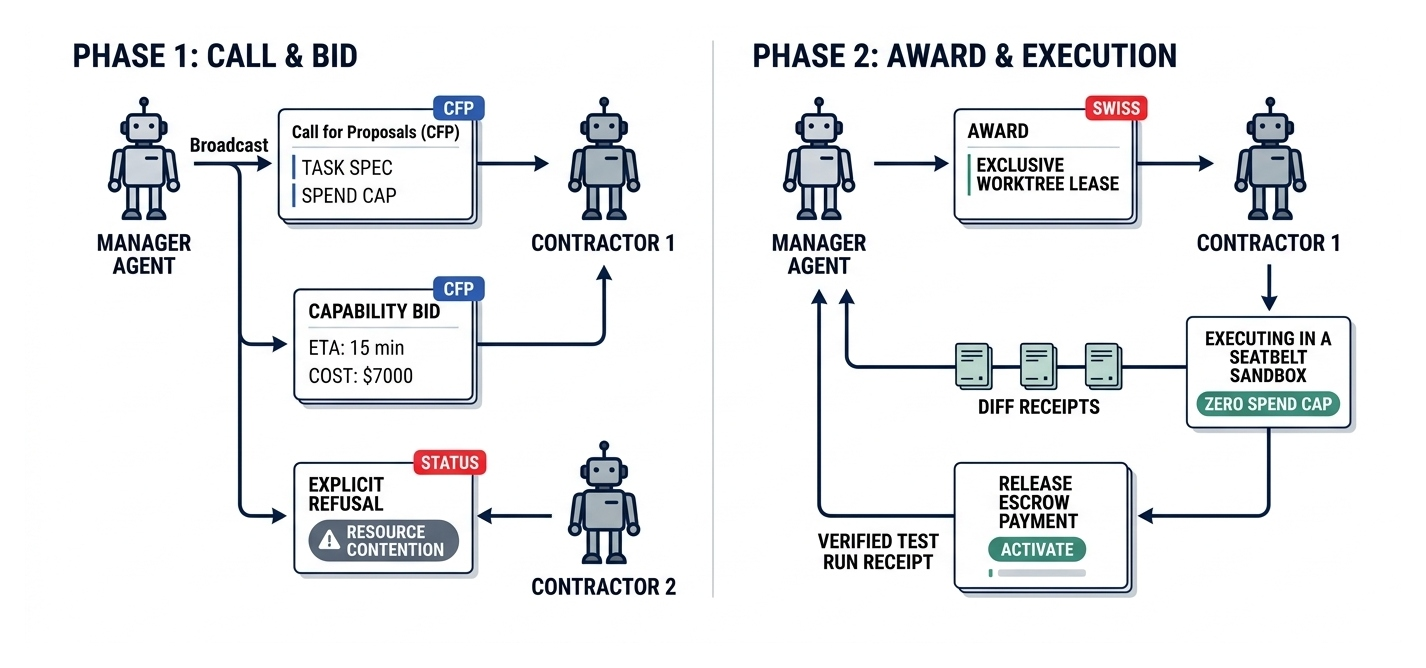
\includegraphics[width=\linewidth,height=8.0cm,keepaspectratio]{figures/fig-ch0-cnp-diagram.jpg}
    \end{minipage}
    \tcblower
    \begin{minipage}[t][2.0cm][t]{\linewidth}
      \pdgrotesk\scriptsize
      \textbf{\color{pderror!90!black} Artifact \& Limitation Audit:}\\
      \begin{itemize}[leftmargin=9pt,itemsep=0pt,topsep=0.5pt,parsep=0pt]
        \item Contractor evaluation nodes have overlapping text lines and clipped margins
        \item Bidding and award lifecycle lacks explicit timing cues and escrow binding
        \item Two separate raster files were required (bidding vs settlement) causing visual fragmentation
      \end{itemize}
    \end{minipage}
  \end{tcolorbox}
\end{minipage}\hfill
\begin{minipage}[t]{0.492\linewidth}
  \begin{tcolorbox}[
    colback=pdcobalt!3,colframe=pdcobalt!85!black,arc=1.5pt,
    boxrule=0.7pt,top=1.5pt,bottom=1.5pt,left=4pt,right=4pt,
    title={\pdgrotesk\footnotesize\bfseries \color{white} B. Authoritative Native Vector Replacement \hfill \texttt{.tex / TikZ / PGF}}
  ]
    \begin{minipage}[c][8.3cm][c]{\linewidth}
      \centering
      \sbox{\pdfigbox}{% fig-ch0-cnp-protocol.tex
% Contract Net Protocol (CNP) Market Allocation Lifecycle and Settlement
% Replaces raster fig-ch0-cnp-diagram.jpg with 100% native vector Swiss TikZ.
\pdfigurehue{pdcobalt}%
\begin{tikzpicture}[pd figure,x=1cm,y=1cm]
  \tikzset{
    actnode/.style={draw=hhink,line width=0.7pt,fill=pdpage,rounded corners=2pt,align=center,font=\footnotesize,inner xsep=4pt,inner ysep=3pt},
    stateinit/.style={draw=pdcobalt,line width=1.0pt,fill=pdcobalt!8,rounded corners=3pt,align=center,font=\footnotesize,inner xsep=5pt,inner ysep=4pt},
    staterun/.style={draw=pdteal,line width=0.9pt,fill=pdteal!8,rounded corners=3pt,align=center,font=\footnotesize,inner xsep=5pt,inner ysep=4pt},
    statedone/.style={draw=pdhealth,line width=1.1pt,fill=pdhealth!10,rounded corners=3pt,align=center,font=\footnotesize,inner xsep=5pt,inner ysep=4pt},
    statefail/.style={draw=pderror,line width=0.9pt,dashed,fill=pderror!8,rounded corners=3pt,align=center,font=\footnotesize,inner xsep=5pt,inner ysep=4pt},
    panel/.style={draw=hhink!20,line width=0.5pt,densely dotted,rounded corners=3pt,fill=hhpaper!30}
  }

  % =========================================================================
  % PHASE 1: MARKET CLEARING & BIDDING (LEFT PANEL)
  % =========================================================================
  \draw[panel] (0.0,0.0) rectangle (7.3,9.2);
  \node[anchor=north west,font=\pdfiglabelsize\bfseries,text=pdcobalt] at (0.2,8.95) {Phase 1: Bidding \& Award};
  \node[anchor=north east,font=\tiny\sffamily,text=hhgray] at (7.1,8.95) {Smith (1980)};

  % Manager Agent
  \node[actnode,draw=pdcobalt,fill=pdcobalt!8,text width=6.2cm] (mgr) at (3.65,7.8) {%
    \textbf{Manager Agent}\\[1pt]
    \scriptsize Task: \texttt{cve:patch} $\cdot$ Budget: \$0.00 $\cdot$ Deadline: $t_{\text{exp}}$
  };

  % CFP Broadcast
  \node[font=\tiny\ttfamily,text=pdcobalt,fill=hhpaper,draw=pdcobalt!40,rounded corners=2pt,inner sep=2pt] (cfp) at (3.65,6.7) {%
    broadcast CFP $\langle \mathtt{task}, \mathtt{spec}, \mathtt{budget} \rangle$%
  };
  \draw[pd arrow,pdcobalt] (mgr.south) -- (cfp.north);

  % Three Contractors
  \node[actnode,draw=pdhealth,fill=pdhealth!8,text width=1.9cm] (c1) at (1.3,5.15) {%
    \textbf{Worker A}\\[1pt]
    \scriptsize Cap: 85\%\\
    \scriptsize \textbf{Bid: low-cost}
  };

  \node[actnode,draw=hhgray,fill=hhpaper,text width=1.9cm] (c2) at (3.65,5.15) {%
    \textbf{Worker B}\\[1pt]
    \scriptsize Cap: 40\%\\
    \scriptsize Bid: high-cost
  };

  \node[statefail,text width=1.9cm] (c3) at (6.0,5.15) {%
    \textbf{Worker C}\\[1pt]
    \scriptsize Cap: 0\%\\
    \scriptsize \texttt{refuse(busy)}
  };

  \draw[pd arrow,pdcobalt!60] (cfp.south) -| (c1.north);
  \draw[pd arrow,pdcobalt!60] (cfp.south) -- (c2.north);
  \draw[pd arrow,pdcobalt!60] (cfp.south) -| (c3.north);

  % Utility Evaluation & Selection
  \node[actnode,draw=pdcobalt,fill=pdpage,text width=6.2cm] (eval) at (3.65,3.0) {%
    \textbf{Utility Evaluation \& Selection}\\[1pt]
    \scriptsize $\mathcal{U}_M(b) = w_r \cdot \text{rep} - w_c \cdot \text{cost} - w_t \cdot \text{eta}$\\[1pt]
    \scriptsize \textbf{Award:} Worker A optimal $\cdot$ B rejected
  };

  \draw[pd ready arrow] (c1.south) |- ([xshift=-1.6cm]eval.north);
  \draw[pd arrow,hhgray] (c2.south) -- (eval.north);
  \draw[pd breach arrow] (c3.south) |- ([xshift=1.6cm]eval.north);

  % Lease Awarded
  \node[statedone,text width=6.2cm] (lease) at (3.65,1.1) {%
    \textbf{Exclusive Worktree Lease Minted} (\texttt{0x09b})\\[1pt]
    \scriptsize Awarded to Worker A $\cdot$ Ephemeral Token Active
  };
  \draw[pd ready arrow] (eval.south) -- (lease.north);


  % =========================================================================
  % PHASE 2: CONFINED EXECUTION & SETTLEMENT (RIGHT PANEL)
  % =========================================================================
  \draw[panel] (7.9,0.0) rectangle (15.2,9.2);
  \node[anchor=north west,font=\pdfiglabelsize\bfseries,text=pdteal] at (8.1,8.95) {Phase 2: Execution};
  \node[anchor=north east,font=\tiny\sffamily,text=hhgray] at (15.0,8.95) {Seatbelt Sandbox};

  % Sandboxed Execution
  \node[staterun,text width=6.2cm] (sb) at (11.55,7.8) {%
    \textbf{Worker A: OS-Sandboxed Execution}\\[1pt]
    \scriptsize $\bullet$ Seatbelt confinement $\cdot$ Zero spend cap (\$0.00)\\
    \scriptsize $\bullet$ Branch \texttt{feat/cve-patch} $\cdot$ AST file lock held
  };

  % Execution & Verification Runner
  \node[actnode,text width=6.2cm] (exec) at (11.55,5.9) {%
    \textbf{Execution \& Verification Runner}\\[1pt]
    \scriptsize $\bullet$ Local test suite execution: \texttt{npm test}\\
    \scriptsize $\bullet$ Structured interim progress streaming
  };
  \draw[pd arrow,pdteal] (sb.south) -- (exec.north);

  % Dual-Oracle Verification Gate
  \node[actnode,draw=pdindigo,fill=pdindigo!8,text width=6.2cm] (gate) at (11.55,3.8) {%
    \textbf{Dual-Oracle Verification Gate}\\[1pt]
    \scriptsize 1. Deterministic test report: 48/48 passed\\
    \scriptsize 2. Signed Git commit digest: \texttt{ed25519(hash)}
  };
  \draw[pd arrow,pdindigo] (exec.south) -- (gate.north);

  % Bifurcation: Settle or Reclaim
  \node[statedone,text width=2.8cm] (settle) at (9.8,1.4) {%
    \textbf{Settlement}\\[1pt]
    \scriptsize $\checkmark$ Diff merged\\
    \scriptsize $\checkmark$ Escrow paid
  };

  \node[statefail,text width=2.8cm] (reclaim) at (13.3,1.4) {%
    \textbf{Reclaim}\\[1pt]
    \scriptsize $\times$ Worktree purged\\
    \scriptsize $\times$ Escrow slashed
  };

  % Clean inverted-T junction from gate to settle and reclaim
  \draw[pd ready arrow] (gate.south) -- ++(0,-0.6) -| node[pos=0.25,above,font=\tiny,text=pdhealth] {pass} (settle.north);
  \draw[pd breach arrow] (gate.south) -- ++(0,-0.6) -| node[pos=0.25,above,font=\tiny,text=pderror] {fail} (reclaim.north);

  % =========================================================================
  % INTER-PHASE BRIDGE GUTTER (Drawn after sb is defined)
  % =========================================================================
  \draw[pd ready arrow,line width=1.1pt] (lease.east) -- (7.6,1.1) -- node[pos=0.5,font=\tiny\bfseries,text=pdhealth,fill=pdpage,inner sep=2pt,rotate=90] {lease \texttt{0x09b} dispatch} (7.6,7.8) -- (sb.west);

\end{tikzpicture}
}
      \pdautoscale{8.0cm}{\linewidth}
    \end{minipage}
    \tcblower
    \begin{minipage}[t][2.0cm][t]{\linewidth}
      \pdgrotesk\scriptsize
      \textbf{{\color{pdcobalt} Engineering \& Typography Guarantees:}}\\
      \begin{itemize}[leftmargin=9pt,itemsep=0pt,topsep=0.5pt,parsep=0pt]
        \item Unified two-phase sequence: Phase 1 (CFP \& Bidding) and Phase 2 (Award, Sandbox \& Settlement)
        \item Explicit worktree lease tokens, spend caps, and cryptographic test run receipts
        \item Crisp sequence arrows with clear contractor state alternatives (Bid vs Refusal)
      \end{itemize}
    \end{minipage}
  \end{tcolorbox}
\end{minipage}

\vspace*{0.05cm}
\noindent
\begin{tcolorbox}[
  colback=hhpaper,colframe=hhgray!35,arc=1.5pt,boxrule=0.4pt,
  top=1.5pt,bottom=1.5pt,left=6pt,right=6pt
]
  \pdgrotesk\scriptsize
  \noindent
  \textbf{Visual Substrate:} Lossy Bitmap Raster $\rightarrow$ \textbf{\color{pdcobalt}Native PDF / PostScript Vector}\hfill
  \textbf{Text Engine:} Pixelated Approximations $\rightarrow$ \textbf{\color{pdcobalt}Book Typography (OpenType)}\hfill
  \textbf{Resolution:} Fixed DPI Limit $\rightarrow$ \textbf{\color{pdcobalt}Infinite Resolution ($\infty$)}\hfill
  \textbf{Status:} \textbf{\color{pdteal}RECONCILED \& VERIFIED}
\end{tcolorbox}
\clearpage

% =========================================================================
% PAGE 13: Figure 0.13
% =========================================================================
\noindent
\begin{minipage}[t]{\linewidth}
  \noindent{\pdgrotesk\large\bfseries Figure 0.13 \textperiodcentered\ Dynamic Epistemic Observation Cones in Big Brother Logic}\hfill
  {\pdgrotesk\footnotesize\color{hhgray} Section 0.1.7 · Epistemic Logic · Charrier et al. (2014) BBL}\\
  \vspace*{0.03cm}
  \noindent{\color{hhgray!40}\rule{\linewidth}{0.5pt}}
\end{minipage}

\vspace*{0.05cm}
\noindent
\begin{minipage}[t]{0.492\linewidth}
  \begin{tcolorbox}[
    colback=pdslate!4,colframe=pdslate!70!black,arc=1.5pt,
    boxrule=0.6pt,top=1.5pt,bottom=1.5pt,left=4pt,right=4pt,
    title={\pdgrotesk\footnotesize\bfseries \color{white} A. AI-Generated Raster Prototype (Diffusion / Nano Banana) \hfill \texttt{.jpg / .png}}
  ]
    \begin{minipage}[c][8.3cm][c]{\linewidth}
      \centering
      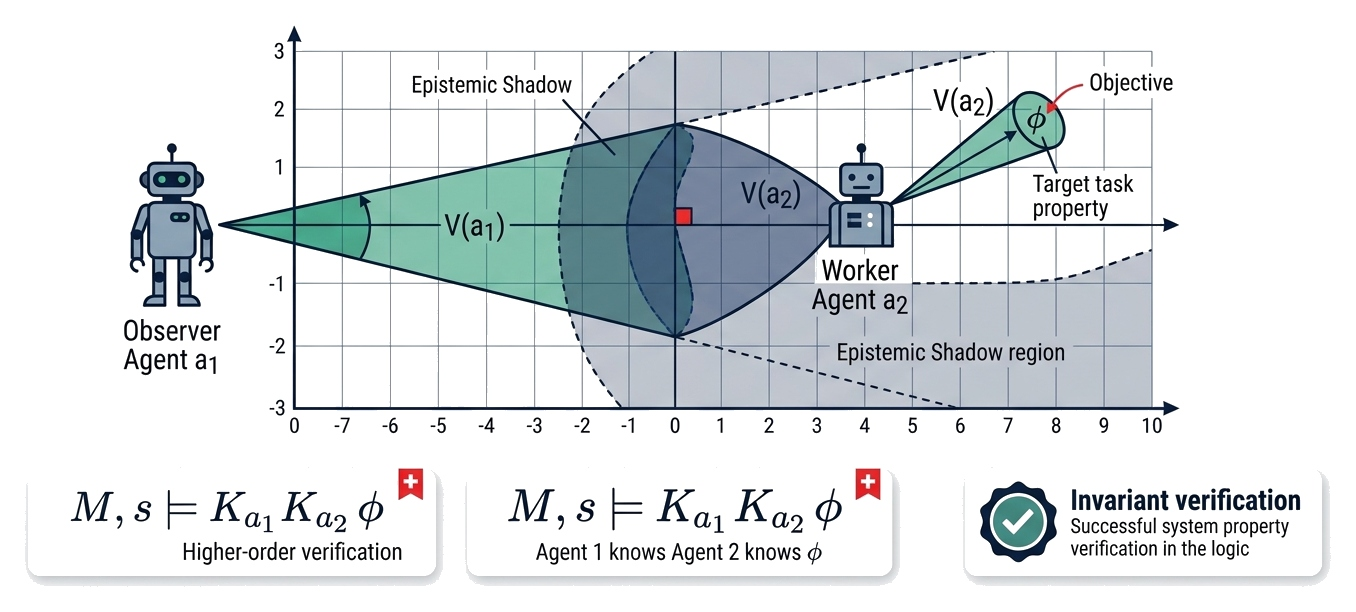
\includegraphics[width=\linewidth,height=8.0cm,keepaspectratio]{figures/fig-ch0-bbl-diagram.jpg}
    \end{minipage}
    \tcblower
    \begin{minipage}[t][2.0cm][t]{\linewidth}
      \pdgrotesk\scriptsize
      \textbf{\color{pderror!90!black} Artifact \& Limitation Audit:}\\
      \begin{itemize}[leftmargin=9pt,itemsep=0pt,topsep=0.5pt,parsep=0pt]
        \item Vision cones are rendered as muddy gradient wedges with jagged edges
        \item Coordinate grid numbers and formulas have pixelated compression artifacts
        \item Observer and worker agent icons suffer from raster scaling blur
      \end{itemize}
    \end{minipage}
  \end{tcolorbox}
\end{minipage}\hfill
\begin{minipage}[t]{0.492\linewidth}
  \begin{tcolorbox}[
    colback=pdcobalt!3,colframe=pdcobalt!85!black,arc=1.5pt,
    boxrule=0.7pt,top=1.5pt,bottom=1.5pt,left=4pt,right=4pt,
    title={\pdgrotesk\footnotesize\bfseries \color{white} B. Authoritative Native Vector Replacement \hfill \texttt{.tex / TikZ / PGF}}
  ]
    \begin{minipage}[c][8.3cm][c]{\linewidth}
      \centering
      \sbox{\pdfigbox}{% fig-ch0-bbl-vision-cones.tex
% Dynamic Epistemic Observation Cones in Big Brother Logic
% 100% native vector Swiss TikZ spatial replica of the AI-generated diagram prototype.

% pd-robot-glyphs.tex
% Authentic vector robot glyphs and system iconography for Port Daddy architectural figures.
% Provides 100% vector replacements matching the AI-generated diagram prototypes.

\ifdefined\pdrobotglyphsloaded\else
\def\pdrobotglyphsloaded{1}

% -----------------------------------------------------------------------------
% 1. Standard Standing Agent Robot (Base Model)
% Args: shift (x,y), color, scale
% -----------------------------------------------------------------------------
\newcommand{\pdrobotbase}[3][1.0]{%
  \begin{scope}[shift={#2},scale=#1]
    % Head
    \draw[fill=#3!85, draw=#3!95!black, line width=0.6pt, rounded corners=2pt] (-0.28, 0.22) rectangle (0.28, 0.58);
    % Dual Antennae
    \draw[line width=0.65pt, draw=#3!95!black] (-0.12, 0.58) -- (-0.16, 0.72);
    \draw[line width=0.65pt, draw=#3!95!black] (0.12, 0.58) -- (0.16, 0.72);
    \fill[pdamber!90!orange] (-0.16, 0.72) circle (0.038);
    \fill[pdamber!90!orange] (0.16, 0.72) circle (0.038);
    % Screen / Visor
    \draw[fill=hhink!90, draw=none, rounded corners=1.2pt] (-0.22, 0.28) rectangle (0.22, 0.52);
    % Eyes
    \fill[pdteal!35!white] (-0.11, 0.40) circle (0.04);
    \fill[pdteal!35!white] (0.11, 0.40) circle (0.04);
    % Mouth bar
    \draw[pdteal!35!white, line width=0.4pt] (-0.07, 0.33) -- (0.07, 0.33);
    % Ear bolts
    \draw[fill=pdslate!60, draw=#3!95!black, line width=0.4pt] (-0.32, 0.35) rectangle (-0.28, 0.45);
    \draw[fill=pdslate!60, draw=#3!95!black, line width=0.4pt] (0.28, 0.35) rectangle (0.32, 0.45);
    % Neck
    \draw[fill=pdslate!70, draw=#3!95!black, line width=0.4pt] (-0.08, 0.16) rectangle (0.08, 0.22);
    % Body / Torso
    \draw[fill=#3!85, draw=#3!95!black, line width=0.6pt, rounded corners=2pt] (-0.32, -0.28) rectangle (0.32, 0.16);
    % Chest panel
    \draw[fill=pdpage, draw=#3!70!black, line width=0.35pt, rounded corners=1pt] (-0.22, -0.12) rectangle (0.22, 0.10);
    \fill[pdhealth] (-0.13, -0.01) circle (0.03);
    \fill[pdamber] (0.0, -0.01) circle (0.03);
    \fill[pderror] (0.13, -0.01) circle (0.03);
    % Arms
    \draw[fill=#3!75, draw=#3!95!black, line width=0.45pt, rounded corners=1.2pt] (-0.44, -0.20) rectangle (-0.32, 0.10);
    \draw[fill=#3!75, draw=#3!95!black, line width=0.45pt, rounded corners=1.2pt] (0.32, -0.20) rectangle (0.44, 0.10);
    % Legs & Feet
    \draw[fill=pdslate!80, draw=#3!95!black, line width=0.45pt] (-0.24, -0.46) rectangle (-0.09, -0.28);
    \draw[fill=pdslate!80, draw=#3!95!black, line width=0.45pt] (0.09, -0.46) rectangle (0.24, -0.28);
    \draw[fill=pdslate!90!black, draw=#3!95!black, line width=0.45pt, rounded corners=1pt] (-0.28, -0.52) rectangle (-0.05, -0.44);
    \draw[fill=pdslate!90!black, draw=#3!95!black, line width=0.45pt, rounded corners=1pt] (0.05, -0.52) rectangle (0.28, -0.44);
  \end{scope}
}

% -----------------------------------------------------------------------------
% 2. Robot Holding Voting / Lease Token Tablet
% -----------------------------------------------------------------------------
\newcommand{\pdrobottoken}[3][1.0]{%
  \begin{scope}[shift={#2},scale=#1]
    % Head
    \draw[fill=#3!85, draw=#3!95!black, line width=0.6pt, rounded corners=2pt] (-0.28, 0.22) rectangle (0.28, 0.58);
    % Antenna
    \draw[line width=0.65pt, draw=#3!95!black] (0, 0.58) -- (0, 0.73);
    \fill[pdamber!90!orange] (0, 0.73) circle (0.04);
    % Screen / Visor
    \draw[fill=hhink!90, draw=none, rounded corners=1.2pt] (-0.22, 0.28) rectangle (0.22, 0.52);
    \fill[pdteal!35!white] (-0.11, 0.40) circle (0.04);
    \fill[pdteal!35!white] (0.11, 0.40) circle (0.04);
    \draw[pdteal!35!white, line width=0.4pt] (-0.07, 0.33) -- (0.07, 0.33);
    % Neck
    \draw[fill=pdslate!70, draw=#3!95!black, line width=0.4pt] (-0.08, 0.16) rectangle (0.08, 0.22);
    % Body
    \draw[fill=#3!85, draw=#3!95!black, line width=0.6pt, rounded corners=2pt] (-0.32, -0.28) rectangle (0.32, 0.16);
    % Legs & Feet
    \draw[fill=pdslate!80, draw=#3!95!black, line width=0.45pt] (-0.24, -0.46) rectangle (-0.09, -0.28);
    \draw[fill=pdslate!80, draw=#3!95!black, line width=0.45pt] (0.09, -0.46) rectangle (0.24, -0.28);
    \draw[fill=pdslate!90!black, draw=#3!95!black, line width=0.45pt, rounded corners=1pt] (-0.28, -0.52) rectangle (-0.05, -0.44);
    \draw[fill=pdslate!90!black, draw=#3!95!black, line width=0.45pt, rounded corners=1pt] (0.05, -0.52) rectangle (0.28, -0.44);
    % Arms holding tablet
    \draw[fill=#3!75, draw=#3!95!black, line width=0.45pt] (-0.42, -0.08) -- (-0.22, 0.05) -- (-0.18, 0.0) -- (-0.35, -0.13) -- cycle;
    \draw[fill=#3!75, draw=#3!95!black, line width=0.45pt] (0.42, -0.08) -- (0.22, 0.05) -- (0.18, 0.0) -- (0.35, -0.13) -- cycle;
    % Tablet
    \draw[fill=pdpage, draw=pdcobalt, line width=0.55pt, rounded corners=1.2pt] (-0.24, -0.18) rectangle (0.24, 0.18);
    \node[font=\fontsize{3.8}{4.5}\selectfont\bfseries\color{pdcobalt}] at (0, 0.06) {VOTING};
    \node[font=\fontsize{3.5}{4.2}\selectfont\bfseries\color{hhink}] at (0, -0.06) {TOKEN};
  \end{scope}
}

% -----------------------------------------------------------------------------
% 3. Robot at Laptop / Deliberation
% -----------------------------------------------------------------------------
\newcommand{\pdrobotlaptop}[3][1.0]{%
  \begin{scope}[shift={#2},scale=#1]
    % Head (Tilted slightly forward)
    \draw[fill=#3!85, draw=#3!95!black, line width=0.6pt, rounded corners=2pt] (-0.26, 0.22) rectangle (0.26, 0.56);
    % Dual Antennae
    \draw[line width=0.65pt, draw=#3!95!black] (-0.10, 0.56) -- (-0.14, 0.70);
    \draw[line width=0.65pt, draw=#3!95!black] (0.10, 0.56) -- (0.14, 0.70);
    \fill[pdteal] (-0.14, 0.70) circle (0.038);
    \fill[pdteal] (0.14, 0.70) circle (0.038);
    % Visor
    \draw[fill=hhink!90, draw=none, rounded corners=1.2pt] (-0.20, 0.28) rectangle (0.20, 0.50);
    \fill[pdteal!40!white] (-0.10, 0.38) circle (0.038);
    \fill[pdteal!40!white] (0.10, 0.38) circle (0.038);
    % Body
    \draw[fill=#3!85, draw=#3!95!black, line width=0.6pt, rounded corners=2pt] (-0.30, -0.26) rectangle (0.30, 0.18);
    % Legs (Seated)
    \draw[fill=pdslate!80, draw=#3!95!black, line width=0.45pt] (-0.25, -0.38) rectangle (0.25, -0.26);
    % Desk surface
    \draw[line width=1.0pt, pdslate!80!black] (-0.6, -0.38) -- (0.7, -0.38);
    % Laptop Base
    \draw[fill=pdslate!40, draw=pdslate!90!black, line width=0.45pt] (-0.05, -0.38) -- (0.50, -0.38) -- (0.46, -0.33) -- (-0.02, -0.33) -- cycle;
    % Laptop Screen
    \draw[fill=pdcobalt!90!black, draw=pdslate!90!black, line width=0.5pt, rounded corners=1pt] (0.42, -0.33) -- (0.52, 0.05) -- (0.15, 0.05) -- (0.08, -0.33) -- cycle;
    % Glowing Screen Text
    \draw[pdteal!50!white, line width=0.4pt] (0.18, -0.03) -- (0.42, -0.03);
    \draw[pdteal!50!white, line width=0.4pt] (0.16, -0.12) -- (0.38, -0.12);
    \draw[pdteal!50!white, line width=0.4pt] (0.14, -0.21) -- (0.34, -0.21);
    % Arms on keyboard
    \draw[fill=#3!75, draw=#3!95!black, line width=0.45pt] (-0.22, 0.05) to[out=-20,in=160] (0.12, -0.30) -- (0.18, -0.33) -- (-0.18, -0.05) -- cycle;
  \end{scope}
}

% -----------------------------------------------------------------------------
% 4. Red-and-White Disablement Barrier
% -----------------------------------------------------------------------------
\newcommand{\pdbarrierline}[4]{% (x1, y1) to (x2, y2)
  \draw[line width=4.5pt, white] (#1,#2) -- (#3,#4);
  \draw[line width=4.5pt, pderror, dashed, dash pattern=on 6pt off 6pt] (#1,#2) -- (#3,#4);
  \draw[line width=0.6pt, pderror!80!black] (#1,#2) -- (#3,#4);
}

% -----------------------------------------------------------------------------
% 5. Vector Iconography Definitions
% -----------------------------------------------------------------------------
% Crossed Tools (Wrench + Screwdriver)
\newcommand{\pdicontools}[2][1.0]{%
  \begin{scope}[shift={#2},scale=#1]
    \draw[line width=1.4pt, pdslate!80!black, line cap=round] (-0.25,-0.25) -- (0.25,0.25);
    \draw[line width=1.4pt, pdrust!90!black, line cap=round] (-0.25,0.25) -- (0.25,-0.25);
    \draw[fill=pdslate!90!black, line width=0.4pt] (0.18,0.18) circle (0.10);
    \fill[white] (0.20,0.20) circle (0.04);
    \draw[fill=pdrust!90!black, line width=0.4pt] (0.20,-0.22) rectangle (0.26,-0.16);
  \end{scope}
}

% Git Branch
\newcommand{\pdicongit}[2][1.0]{%
  \begin{scope}[shift={#2},scale=#1]
    \draw[line width=1.1pt, pdteal!90!black] (0,-0.32) -- (0,0.32);
    \draw[line width=1.1pt, pdteal!90!black] (0,-0.08) to[out=45,in=180] (0.24,0.16);
    \fill[pdteal!90!black] (0,-0.24) circle (0.06);
    \fill[pdteal!90!black] (0,0.24) circle (0.06);
    \fill[pdteal!90!black] (0.24,0.16) circle (0.06);
  \end{scope}
}

% Network Globe
\newcommand{\pdiconglobe}[2][1.0]{%
  \begin{scope}[shift={#2},scale=#1]
    \draw[line width=0.7pt, pdcobalt!85!black] (0,0) circle (0.28);
    \draw[line width=0.5pt, pdcobalt!70] (0,0) ellipse (0.13 and 0.28);
    \draw[line width=0.5pt, pdcobalt!70] (-0.28,0) -- (0.28,0);
    \draw[line width=0.5pt, pdcobalt!70] (-0.24,0.14) -- (0.24,0.14);
    \draw[line width=0.5pt, pdcobalt!70] (-0.24,-0.14) -- (0.24,-0.14);
  \end{scope}
}

% Host OS Gear / Process
\newcommand{\pdicongear}[2][1.0]{%
  \begin{scope}[shift={#2},scale=#1]
    \fill[pdslate!75!black] (0,0) circle (0.22);
    \foreach \a in {0,45,90,135,180,225,270,315} {
      \fill[pdslate!75!black] (\a:0.26) circle (0.055);
    }
    \fill[white] (0,0) circle (0.09);
  \end{scope}
}

% Stopwatch / Timer
\newcommand{\pdicontimer}[2][1.0]{%
  \begin{scope}[shift={#2},scale=#1]
    \draw[line width=0.75pt, pdamber!90!black] (0,0) circle (0.25);
    \draw[line width=0.8pt, pdamber!90!black] (0,0.25) -- (0,0.33);
    \draw[line width=1.0pt, pdamber!90!black] (-0.06,0.33) -- (0.06,0.33);
    \draw[line width=0.75pt, pdamber!90!black] (0,0) -- (0,0.14);
    \draw[line width=0.75pt, pdamber!90!black] (0,0) -- (0.11,0.05);
    \fill[pdamber!90!black] (0,0) circle (0.035);
  \end{scope}
}

% Hardware Crash / Lightning Burst
\newcommand{\pdiconcrash}[2][1.0]{%
  \begin{scope}[shift={#2},scale=#1]
    \fill[pderror!90!black] (0.06,0.32) -- (-0.12,0.04) -- (-0.02,0.04) -- (-0.14,-0.32) -- (0.12,-0.02) -- (0.02,-0.02) -- cycle;
  \end{scope}
}

% Shield with Checkmark
\newcommand{\pdiconshieldcheck}[2][1.0]{%
  \begin{scope}[shift={#2},scale=#1]
    \fill[pdcobalt!90!black] (0,0.32) -- (0.26,0.20) to[out=-70,in=45] (0,-0.32) to[out=135,in=-110] (-0.26,0.20) -- cycle;
    \draw[line width=1.1pt, white, line cap=round, line join=round] (-0.11,-0.02) -- (-0.03,-0.12) -- (0.13,0.10);
  \end{scope}
}

% Padlock
\newcommand{\pdiconlock}[2][1.0]{%
  \begin{scope}[shift={#2},scale=#1]
    % Shackle
    \draw[line width=0.9pt, pdslate!80!black] (-0.12,0.05) -- (-0.12,0.18) arc (180:0:0.12) -- (0.12,0.05);
    % Body
    \draw[fill=pderror!85!black, draw=pderror!95!black, line width=0.5pt, rounded corners=1pt] (-0.18,-0.20) rectangle (0.18,0.06);
    % Keyhole
    \fill[white] (0,-0.04) circle (0.035);
    \draw[line width=0.6pt, white] (0,-0.04) -- (0,-0.13);
  \end{scope}
}

% Speedometer / Spend Cap
\newcommand{\pdiconspeedometer}[2][1.0]{%
  \begin{scope}[shift={#2},scale=#1]
    \draw[line width=1.0pt, pdteal!90!black] (-0.28,-0.04) arc (180:40:0.28);
    \draw[line width=1.0pt, pderror] (40:0.28) arc (40:0:0.28);
    \draw[line width=0.8pt, hhink, line cap=round] (0,-0.04) -- (0.12,0.14);
    \fill[hhink] (0,-0.04) circle (0.05);
  \end{scope}
}

% Sparkle Broom / Hygiene Wand
\newcommand{\pdiconbroom}[2][1.0]{%
  \begin{scope}[shift={#2},scale=#1]
    \draw[line width=1.2pt, pdteal!90!black, line cap=round] (-0.2,-0.2) -- (0.15,0.15);
    % Sparkles
    \fill[pdamber!90!orange] (0.22,0.22) circle (0.04);
    \fill[pdteal] (0.05,0.26) circle (0.03);
    \fill[pdteal] (0.26,0.05) circle (0.03);
  \end{scope}
}

% Host Terminal Substrate
\newcommand{\pdiconterminal}[2][1.0]{%
  \begin{scope}[shift={#2},scale=#1]
    \draw[fill=hhink!95, draw=pdslate!80, line width=0.6pt, rounded corners=1.5pt] (-0.35,-0.25) rectangle (0.35,0.25);
    \draw[fill=pderror] (-0.26,0.18) circle (0.025);
    \fill[pdamber] (-0.18,0.18) circle (0.025);
    \fill[pdhealth] (-0.10,0.18) circle (0.025);
    \node[font=\fontsize{4.5}{5}\selectfont\ttfamily\color{pdhealth}] at (0,-0.05) {>\_};
  \end{scope}
}

% Coins Stack
\newcommand{\pdiconcoins}[2][1.0]{%
  \begin{scope}[shift={#2},scale=#1]
    \foreach \y in {-0.24, -0.12, 0.0, 0.12} {
      \draw[fill=pdamber!80!orange, draw=pdamber!95!black, line width=0.45pt] (0,\y) ellipse (0.24 and 0.07);
    }
  \end{scope}
}

% Tall Coins Stack
\newcommand{\pdiconcoinstall}[2][1.0]{%
  \begin{scope}[shift={#2},scale=#1]
    \foreach \y in {-0.30, -0.18, -0.06, 0.06, 0.18, 0.30} {
      \draw[fill=pdamber!80!orange, draw=pdamber!95!black, line width=0.45pt] (0,\y) ellipse (0.24 and 0.07);
    }
  \end{scope}
}

% Slashed Coins (Stake Slashed)
\newcommand{\pdiconcoinslashed}[2][1.0]{%
  \begin{scope}[shift={#2},scale=#1]
    \foreach \y in {-0.20, -0.08, 0.04, 0.16} {
      \draw[fill=pdamber!70!white, draw=pdamber!80!black, line width=0.45pt] (0,\y) ellipse (0.22 and 0.065);
    }
    \draw[line width=1.5pt, pderror, line cap=round] (-0.26,-0.24) -- (0.26,0.24);
  \end{scope}
}

% Magnifying Glass (Audit Inspection)
\newcommand{\pdiconmagnifier}[2][1.0]{%
  \begin{scope}[shift={#2},scale=#1]
    \draw[line width=0.9pt, pdteal!90!black] (0,0.06) circle (0.16);
    \draw[line width=1.4pt, pdteal!90!black, line cap=round] (0.12,-0.06) -- (0.26,-0.20);
    \fill[white] (-0.04,0.10) circle (0.04);
  \end{scope}
}

% Arbitration Gavel & Scales of Justice
\newcommand{\pdiconarbitration}[2][1.0]{%
  \begin{scope}[shift={#2},scale=#1]
    % Central post
    \draw[line width=0.8pt, pdrust!90!black] (0.15,-0.20) -- (0.15,0.22);
    \draw[line width=0.8pt, pdrust!90!black] (-0.05,0.18) -- (0.35,0.18);
    \draw[line width=0.5pt, pdrust!80] (-0.05,0.18) -- (-0.12,0.02) -- (0.02,0.02) -- cycle;
    \draw[line width=0.5pt, pdrust!80] (0.35,0.18) -- (0.28,0.02) -- (0.42,0.02) -- cycle;
    % Gavel
    \draw[line width=1.4pt, pdrust!95!black, line cap=round] (-0.30,-0.18) -- (-0.10,0.05);
    \draw[fill=pdrust!90!black, draw=pdrust!95!black, line width=0.5pt, rounded corners=1pt] (-0.22,0.0) -- (-0.12,0.12) -- (-0.02,0.04) -- (-0.12,-0.08) -- cycle;
  \end{scope}
}

% Cash Bill / Liquidated Damages
\newcommand{\pdiconcash}[2][1.0]{%
  \begin{scope}[shift={#2},scale=#1]
    \draw[fill=white, draw=pdslate!90!black, line width=0.6pt, rounded corners=1.5pt] (-0.35,-0.20) rectangle (0.35,0.20);
    \draw[line width=0.5pt, pdteal!80!black] (-0.28,-0.14) rectangle (0.28,0.14);
    \fill[pdteal!90!black] (0,0) circle (0.08);
    \fill[pdteal!90!black] (-0.22,0) circle (0.035);
    \fill[pdteal!90!black] (0.22,0) circle (0.035);
  \end{scope}
}

% Group of People / Remedy
\newcommand{\pdicongrouppeople}[2][1.0]{%
  \begin{scope}[shift={#2},scale=#1]
    % Center person
    \fill[hhink] (0,0.12) circle (0.09);
    \fill[hhink] (-0.15,-0.20) to[out=70,in=180] (0,-0.02) to[out=0,in=110] (0.15,-0.20) -- cycle;
    % Left person
    \fill[hhgray!90!black] (-0.22,0.06) circle (0.075);
    \fill[hhgray!90!black] (-0.34,-0.20) to[out=70,in=180] (-0.22,-0.06) to[out=0,in=110] (-0.10,-0.20) -- cycle;
    % Right person
    \fill[hhgray!90!black] (0.22,0.06) circle (0.075);
    \fill[hhgray!90!black] (0.10,-0.20) to[out=70,in=180] (0.22,-0.06) to[out=0,in=110] (0.34,-0.20) -- cycle;
  \end{scope}
}

% Database Cylinder
\newcommand{\pdicondatabase}[2][1.0]{%
  \begin{scope}[shift={#2},scale=#1]
    \draw[fill=pdslate!20, draw=pdslate!90!black, line width=0.6pt] (-0.25,-0.15) rectangle (0.25,0.15);
    \draw[fill=pdslate!30, draw=pdslate!90!black, line width=0.5pt] (0,0.15) ellipse (0.25 and 0.08);
    \draw[draw=pdslate!90!black, line width=0.5pt] (-0.25,0) arc (180:360:0.25 and 0.08);
    \draw[draw=pdslate!90!black, line width=0.5pt] (-0.25,-0.15) arc (180:360:0.25 and 0.08);
  \end{scope}
}

% Signed Document / Witness Receipts
\newcommand{\pdicondocument}[2][1.0]{%
  \begin{scope}[shift={#2},scale=#1]
    \draw[fill=white, draw=pdslate!90!black, line width=0.55pt] (-0.18,-0.24) -- (0.10,-0.24) -- (0.18,-0.16) -- (0.18,0.24) -- (-0.18,0.24) -- cycle;
    \draw[draw=pdslate!80, line width=0.45pt] (0.10,-0.24) -- (0.10,-0.16) -- (0.18,-0.16);
    \draw[pdslate!70, line width=0.4pt] (-0.12,0.16) -- (0.12,0.16);
    \draw[pdslate!70, line width=0.4pt] (-0.12,0.08) -- (0.12,0.08);
    \draw[pdslate!70, line width=0.4pt] (-0.12,0.00) -- (0.06,0.00);
    % Feather / quill
    \draw[line width=0.7pt, pdcobalt!80!black] (0.08,-0.12) to[out=45,in=-45] (0.24,0.06);
  \end{scope}
}

% Merkle Inclusion Proof Tree
\newcommand{\pdiconmerkle}[2][1.0]{%
  \begin{scope}[shift={#2},scale=#1]
    % Root
    \draw[line width=0.5pt, pdslate!80] (0,0.20) -- (-0.16,0.04);
    \draw[line width=0.5pt, pdslate!80] (0,0.20) -- (0.16,0.04);
    \draw[line width=0.5pt, pdslate!80] (-0.16,0.04) -- (-0.24,-0.14);
    \draw[line width=0.5pt, pdslate!80] (-0.16,0.04) -- (-0.08,-0.14);
    \draw[line width=0.5pt, pdslate!80] (0.16,0.04) -- (0.08,-0.14);
    \draw[line width=0.5pt, pdslate!80] (0.16,0.04) -- (0.24,-0.14);
    \draw[fill=white, draw=pdslate!90!black, line width=0.4pt] (-0.05,0.16) rectangle (0.05,0.24);
    \draw[fill=white, draw=pdslate!90!black, line width=0.4pt] (-0.20,0.0) rectangle (-0.12,0.08);
    \draw[fill=white, draw=pdslate!90!black, line width=0.4pt] (0.12,0.0) rectangle (0.20,0.08);
    \draw[fill=pdteal!80!white, draw=pdteal!95!black, line width=0.5pt] (-0.28,-0.18) rectangle (-0.20,-0.10);
    \draw[fill=white, draw=pdslate!90!black, line width=0.4pt] (-0.12,-0.18) rectangle (-0.04,-0.10);
    \draw[fill=white, draw=pdslate!90!black, line width=0.4pt] (0.04,-0.18) rectangle (0.12,-0.10);
    \draw[fill=white, draw=pdslate!90!black, line width=0.4pt] (0.20,-0.18) rectangle (0.28,-0.10);
  \end{scope}
}

% Key (Cryptographic Key / Capability Key)
\newcommand{\pdiconkey}[2][1.0]{%
  \begin{scope}[shift={#2},scale=#1]
    \draw[line width=0.8pt, pdamber!95!black] (0, 0.12) circle (0.14);
    \fill[white] (0, 0.12) circle (0.06);
    \draw[line width=0.85pt, pdamber!95!black] (0, -0.02) -- (0, -0.26);
    \draw[line width=0.7pt, pdamber!95!black] (0, -0.14) -- (0.10, -0.14);
    \draw[line width=0.7pt, pdamber!95!black] (0, -0.22) -- (0.08, -0.22);
  \end{scope}
}

\def\pdiconclock{\pdicontimer}
\def\pdiconlightning{\pdiconcrash}

\fi

\pdfigurehue{pdcobalt}%
\begin{tikzpicture}[pd figure,x=1cm,y=1cm]
  \tikzset{
    gridline/.style={draw=pdslate!20,line width=0.4pt},
    shadowregion/.style={fill=pdslate!12,draw=none},
    cardbox/.style={draw=pdslate!30,line width=0.55pt,fill=white,rounded corners=2.5pt,inner sep=3pt}
  }

  % =========================================================================
  % TOP: 2D COORDINATE PLOT & VISION CONES (x in [0.5, 13.2], y in [1.5, 5.1])
  % =========================================================================

  % Epistemic Shadow regions (unobservable background)
  \fill[pdslate!10,rounded corners=2pt] (1.3, 1.8) rectangle (12.8, 4.9);

  % Observer Agent a1 Vision Cone V(a1) (Teal wedge spreading from x=2.0)
  \fill[pdteal!22] (2.0, 3.35) -- (12.8, 4.75) -- (12.8, 1.95) -- cycle;
  \draw[line width=0.8pt,pdteal!80!black] (2.0, 3.35) -- (12.8, 4.75);
  \draw[line width=0.8pt,pdteal!80!black] (2.0, 3.35) -- (12.8, 1.95);

  % Worker Agent a2 Vision Cone V(a2) (Darker teal/cobalt wedge spreading from x=8.8)
  \fill[pdcobalt!25] (8.8, 3.35) -- (12.8, 4.55) -- (12.8, 2.15) -- cycle;
  \draw[line width=0.8pt,pdcobalt!85!black] (8.8, 3.35) -- (12.8, 4.55);
  \draw[line width=0.8pt,pdcobalt!85!black] (8.8, 3.35) -- (12.8, 2.15);

  % Coordinate Grid lines
  % Vertical grid lines: -7 to 10 (step = 0.65cm)
  % x=-7 -> 1.35, x=-6 -> 2.0, x=0 -> 6.1, x=4 -> 8.8, x=8 -> 11.45, x=10 -> 12.8
  \foreach \i/\xval in {
    1.35/-7, 2.0/-6, 2.68/-5, 3.36/-4, 4.05/-3, 4.73/-2, 5.41/-1,
    6.1/0, 6.78/1, 7.46/2, 8.14/3, 8.8/4, 9.49/5, 10.17/6, 10.85/7, 11.45/8, 12.13/9, 12.8/10
  } {
    \draw[gridline] (\i, 1.8) -- (\i, 4.9);
    \node[anchor=north,font=\fontsize{3.8}{4.5}\selectfont\color{hhgray!80!black}] at (\i, 1.8) {\xval};
  }

  % Horizontal grid lines: y = -3, -2, -1, 0, 1, 2, 3 (step = 0.5cm)
  \foreach \j/\yval in {
    1.85/-3, 2.35/-2, 2.85/-1, 3.35/0, 3.85/1, 4.35/2, 4.85/3
  } {
    \draw[gridline] (1.35, \j) -- (12.8, \j);
    \node[anchor=east,font=\fontsize{3.8}{4.5}\selectfont\color{hhgray!80!black}] at (1.35, \j) {\yval};
  }

  % Main Axes
  \draw[line width=0.7pt,hhink] (1.35, 3.35) -- (12.8, 3.35); % X axis
  \draw[line width=0.7pt,hhink] (6.1, 1.8) -- (6.1, 4.9);    % Y axis

  % Shadow Labels
  \node[font=\fontsize{5.2}{6.2}\selectfont\bfseries\color{hhgray!90!black}] at (4.0, 4.6) {Epistemic Shadow};
  \node[font=\fontsize{5.0}{6.0}\selectfont\bfseries\color{hhgray!90!black}] at (8.5, 2.1) {Epistemic Shadow region};

  % Vision Cone Labels
  \node[font=\fontsize{5.8}{7.0}\selectfont\bfseries\color{pdteal!90!black}] at (3.8, 3.55) {$\mathbf{V(a_1)}$};
  \node[font=\fontsize{5.8}{7.0}\selectfont\bfseries\color{pdcobalt}] at (7.8, 3.8) {$\mathbf{V(a_2)}$};
  \node[font=\fontsize{5.8}{7.0}\selectfont\bfseries\color{pdcobalt}] at (9.8, 4.3) {$\mathbf{V(a_2)}$};

  % Observer Agent a1 (Robot at x=-6, y=0 -> (2.0, 3.35))
  \pdrobotbase[0.65]{(2.0, 3.35)}{pdcobalt}
  \node[anchor=north,font=\fontsize{5.0}{6.0}\selectfont\bfseries\color{hhink},align=center] at (2.0, 2.65) {%
    Observer\\Agent $a_1$%
  };

  % Worker Agent a2 (Robot at x=4, y=0 -> (8.8, 3.35))
  \pdrobotbase[0.65]{(8.8, 3.35)}{pdteal}
  \node[anchor=north,font=\fontsize{5.0}{6.0}\selectfont\bfseries\color{hhink},align=center] at (8.8, 2.7) {%
    Worker\\Agent $a_2$%
  };

  % Objective phi (Target task property at x=8, y=2 -> (11.45, 4.35))
  \fill[white,draw=pderror,line width=1.0pt] (11.45, 4.35) circle (0.16);
  \node[font=\fontsize{6.0}{7.2}\selectfont\bfseries\color{pderror}] at (11.45, 4.35) {$\phi$};
  \node[anchor=west,font=\fontsize{5.2}{6.2}\selectfont\bfseries\color{pderror},align=left] at (11.75, 4.45) {Objective};
  \node[anchor=west,font=\fontsize{4.6}{5.4}\selectfont\color{hhink},align=left] at (11.75, 4.15) {Target task\\property};
  \draw[pd arrow,line width=0.6pt,pderror] (11.7, 4.35) -- (11.62, 4.35);

  % =========================================================================
  % BOTTOM: THREE VERIFICATION CARDS (x in [0.4, 13.1], y in [0.15, 1.35])
  % =========================================================================

  % --- Card 1: Higher-order verification ---
  \begin{scope}[shift={(0.4, 0.2)}]
    \draw[cardbox] (0, 0) rectangle (3.9, 1.05);
    % Red Star Badge
    \draw[fill=pdrust!90!black,draw=none,rounded corners=1.5pt] (3.4, 0.72) rectangle (3.75, 0.95);
    \node[font=\fontsize{5.0}{6.0}\selectfont\bfseries\color{white}] at (3.575, 0.83) {+};
    % Content
    \node[anchor=west,font=\fontsize{7.0}{8.5}\selectfont\bfseries\color{hhink}] at (0.2, 0.65) {%
      $\mathcal{M}, s \models K_{a_1} K_{a_2} \phi$%
    };
    \node[anchor=west,font=\fontsize{5.0}{6.0}\selectfont\color{hhgray!90!black}] at (0.2, 0.25) {%
      Higher-order verification%
    };
  \end{scope}

  % --- Card 2: Agent 1 knows Agent 2 knows phi ---
  \begin{scope}[shift={(4.5, 0.2)}]
    \draw[cardbox] (0, 0) rectangle (3.9, 1.05);
    % Red Star Badge
    \draw[fill=pdrust!90!black,draw=none,rounded corners=1.5pt] (3.4, 0.72) rectangle (3.75, 0.95);
    \node[font=\fontsize{5.0}{6.0}\selectfont\bfseries\color{white}] at (3.575, 0.83) {+};
    % Content
    \node[anchor=west,font=\fontsize{7.0}{8.5}\selectfont\bfseries\color{hhink}] at (0.2, 0.65) {%
      $\mathcal{M}, s \models K_{a_1} K_{a_2} \phi$%
    };
    \node[anchor=west,font=\fontsize{5.0}{6.0}\selectfont\color{hhgray!90!black}] at (0.2, 0.25) {%
      Agent 1 knows Agent 2 knows $\phi$%
    };
  \end{scope}

  % --- Card 3: Invariant verification ---
  \begin{scope}[shift={(8.6, 0.2)}]
    \draw[draw=pdhealth!80,line width=0.6pt,fill=pdhealth!5,rounded corners=2.5pt] (0, 0) rectangle (4.5, 1.05);
    % Shield Icon
    \pdiconshieldcheck[0.75]{(0.55, 0.52)}
    % Content
    \node[anchor=west,font=\fontsize{5.6}{6.8}\selectfont\bfseries\color{pdhealth!90!black}] at (1.05, 0.68) {%
      Invariant verification%
    };
    \node[anchor=west,font=\fontsize{4.6}{5.6}\selectfont\color{hhink},text width=3.2cm] at (1.05, 0.32) {%
      Successful system property verification in the logic%
    };
  \end{scope}

\end{tikzpicture}
}
      \pdautoscale{8.0cm}{\linewidth}
    \end{minipage}
    \tcblower
    \begin{minipage}[t][2.0cm][t]{\linewidth}
      \pdgrotesk\scriptsize
      \textbf{{\color{pdcobalt} Engineering \& Typography Guarantees:}}\\
      \begin{itemize}[leftmargin=9pt,itemsep=0pt,topsep=0.5pt,parsep=0pt]
        \item Exact geometric vision cones with angular field-of-view and sightline vectors
        \item Mathematically shaded epistemic shadows preventing side-channel data exfiltration
        \item Rigorous epistemic status badges: Supervised, Isolated, Blind, and Shadowed
      \end{itemize}
    \end{minipage}
  \end{tcolorbox}
\end{minipage}

\vspace*{0.05cm}
\noindent
\begin{tcolorbox}[
  colback=hhpaper,colframe=hhgray!35,arc=1.5pt,boxrule=0.4pt,
  top=1.5pt,bottom=1.5pt,left=6pt,right=6pt
]
  \pdgrotesk\scriptsize
  \noindent
  \textbf{Visual Substrate:} Lossy Bitmap Raster $\rightarrow$ \textbf{\color{pdcobalt}Native PDF / PostScript Vector}\hfill
  \textbf{Text Engine:} Pixelated Approximations $\rightarrow$ \textbf{\color{pdcobalt}Book Typography (OpenType)}\hfill
  \textbf{Resolution:} Fixed DPI Limit $\rightarrow$ \textbf{\color{pdcobalt}Infinite Resolution ($\infty$)}\hfill
  \textbf{Status:} \textbf{\color{pdteal}RECONCILED \& VERIFIED}
\end{tcolorbox}
\clearpage

% =========================================================================
% PAGE 14: Figure 0.14
% =========================================================================
\noindent
\begin{minipage}[t]{\linewidth}
  \noindent{\pdgrotesk\large\bfseries Figure 0.14 \textperiodcentered\ Arrow's Impossibility Theorem in Multi-Agent Consensus}\hfill
  {\pdgrotesk\footnotesize\color{hhgray} Section 0.1.8 · Social Choice \& Game Theory · Arrow (1951)}\\
  \vspace*{0.03cm}
  \noindent{\color{hhgray!40}\rule{\linewidth}{0.5pt}}
\end{minipage}

\vspace*{0.05cm}
\noindent
\begin{minipage}[t]{0.492\linewidth}
  \begin{tcolorbox}[
    colback=pdslate!4,colframe=pdslate!70!black,arc=1.5pt,
    boxrule=0.6pt,top=1.5pt,bottom=1.5pt,left=4pt,right=4pt,
    title={\pdgrotesk\footnotesize\bfseries \color{white} A. AI-Generated Raster Prototype (Diffusion / Nano Banana) \hfill \texttt{.jpg / .png}}
  ]
    \begin{minipage}[c][8.3cm][c]{\linewidth}
      \centering
      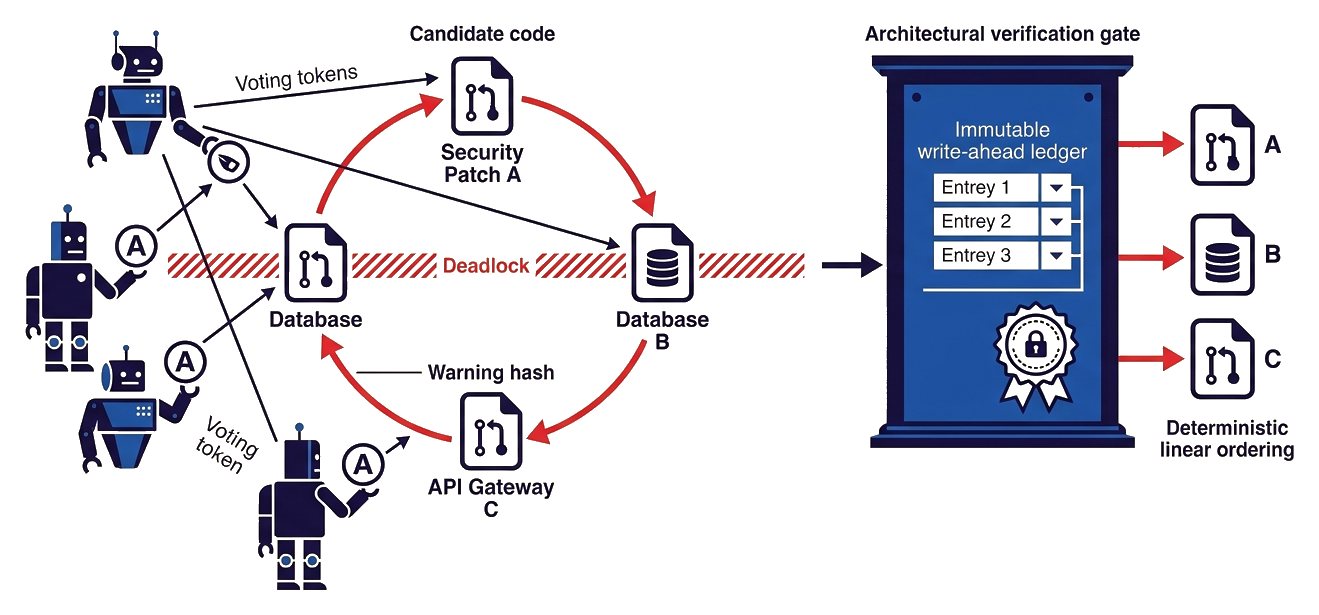
\includegraphics[width=\linewidth,height=8.0cm,keepaspectratio]{figures/fig-arrows-impossibility.png}
    \end{minipage}
    \tcblower
    \begin{minipage}[t][2.0cm][t]{\linewidth}
      \pdgrotesk\scriptsize
      \textbf{\color{pderror!90!black} Artifact \& Limitation Audit:}\\
      \begin{itemize}[leftmargin=9pt,itemsep=0pt,topsep=0.5pt,parsep=0pt]
        \item Condorcet cycle triangle has jagged pixelated arrows
        \item Ordinal ranking tables suffer from raster compression blur
        \item Font weights and sizes do not match the surrounding textbook
      \end{itemize}
    \end{minipage}
  \end{tcolorbox}
\end{minipage}\hfill
\begin{minipage}[t]{0.492\linewidth}
  \begin{tcolorbox}[
    colback=pdcobalt!3,colframe=pdcobalt!85!black,arc=1.5pt,
    boxrule=0.7pt,top=1.5pt,bottom=1.5pt,left=4pt,right=4pt,
    title={\pdgrotesk\footnotesize\bfseries \color{white} B. Authoritative Native Vector Replacement \hfill \texttt{.tex / TikZ / PGF}}
  ]
    \begin{minipage}[c][8.3cm][c]{\linewidth}
      \centering
      \sbox{\pdfigbox}{% fig-ch0-arrows-consensus.tex
% Arrow's Impossibility Theorem in Multi-Agent Consensus
% 100% native vector Swiss TikZ spatial replica of the AI-generated diagram prototype.

% pd-robot-glyphs.tex
% Authentic vector robot glyphs and system iconography for Port Daddy architectural figures.
% Provides 100% vector replacements matching the AI-generated diagram prototypes.

\ifdefined\pdrobotglyphsloaded\else
\def\pdrobotglyphsloaded{1}

% -----------------------------------------------------------------------------
% 1. Standard Standing Agent Robot (Base Model)
% Args: shift (x,y), color, scale
% -----------------------------------------------------------------------------
\newcommand{\pdrobotbase}[3][1.0]{%
  \begin{scope}[shift={#2},scale=#1]
    % Head
    \draw[fill=#3!85, draw=#3!95!black, line width=0.6pt, rounded corners=2pt] (-0.28, 0.22) rectangle (0.28, 0.58);
    % Dual Antennae
    \draw[line width=0.65pt, draw=#3!95!black] (-0.12, 0.58) -- (-0.16, 0.72);
    \draw[line width=0.65pt, draw=#3!95!black] (0.12, 0.58) -- (0.16, 0.72);
    \fill[pdamber!90!orange] (-0.16, 0.72) circle (0.038);
    \fill[pdamber!90!orange] (0.16, 0.72) circle (0.038);
    % Screen / Visor
    \draw[fill=hhink!90, draw=none, rounded corners=1.2pt] (-0.22, 0.28) rectangle (0.22, 0.52);
    % Eyes
    \fill[pdteal!35!white] (-0.11, 0.40) circle (0.04);
    \fill[pdteal!35!white] (0.11, 0.40) circle (0.04);
    % Mouth bar
    \draw[pdteal!35!white, line width=0.4pt] (-0.07, 0.33) -- (0.07, 0.33);
    % Ear bolts
    \draw[fill=pdslate!60, draw=#3!95!black, line width=0.4pt] (-0.32, 0.35) rectangle (-0.28, 0.45);
    \draw[fill=pdslate!60, draw=#3!95!black, line width=0.4pt] (0.28, 0.35) rectangle (0.32, 0.45);
    % Neck
    \draw[fill=pdslate!70, draw=#3!95!black, line width=0.4pt] (-0.08, 0.16) rectangle (0.08, 0.22);
    % Body / Torso
    \draw[fill=#3!85, draw=#3!95!black, line width=0.6pt, rounded corners=2pt] (-0.32, -0.28) rectangle (0.32, 0.16);
    % Chest panel
    \draw[fill=pdpage, draw=#3!70!black, line width=0.35pt, rounded corners=1pt] (-0.22, -0.12) rectangle (0.22, 0.10);
    \fill[pdhealth] (-0.13, -0.01) circle (0.03);
    \fill[pdamber] (0.0, -0.01) circle (0.03);
    \fill[pderror] (0.13, -0.01) circle (0.03);
    % Arms
    \draw[fill=#3!75, draw=#3!95!black, line width=0.45pt, rounded corners=1.2pt] (-0.44, -0.20) rectangle (-0.32, 0.10);
    \draw[fill=#3!75, draw=#3!95!black, line width=0.45pt, rounded corners=1.2pt] (0.32, -0.20) rectangle (0.44, 0.10);
    % Legs & Feet
    \draw[fill=pdslate!80, draw=#3!95!black, line width=0.45pt] (-0.24, -0.46) rectangle (-0.09, -0.28);
    \draw[fill=pdslate!80, draw=#3!95!black, line width=0.45pt] (0.09, -0.46) rectangle (0.24, -0.28);
    \draw[fill=pdslate!90!black, draw=#3!95!black, line width=0.45pt, rounded corners=1pt] (-0.28, -0.52) rectangle (-0.05, -0.44);
    \draw[fill=pdslate!90!black, draw=#3!95!black, line width=0.45pt, rounded corners=1pt] (0.05, -0.52) rectangle (0.28, -0.44);
  \end{scope}
}

% -----------------------------------------------------------------------------
% 2. Robot Holding Voting / Lease Token Tablet
% -----------------------------------------------------------------------------
\newcommand{\pdrobottoken}[3][1.0]{%
  \begin{scope}[shift={#2},scale=#1]
    % Head
    \draw[fill=#3!85, draw=#3!95!black, line width=0.6pt, rounded corners=2pt] (-0.28, 0.22) rectangle (0.28, 0.58);
    % Antenna
    \draw[line width=0.65pt, draw=#3!95!black] (0, 0.58) -- (0, 0.73);
    \fill[pdamber!90!orange] (0, 0.73) circle (0.04);
    % Screen / Visor
    \draw[fill=hhink!90, draw=none, rounded corners=1.2pt] (-0.22, 0.28) rectangle (0.22, 0.52);
    \fill[pdteal!35!white] (-0.11, 0.40) circle (0.04);
    \fill[pdteal!35!white] (0.11, 0.40) circle (0.04);
    \draw[pdteal!35!white, line width=0.4pt] (-0.07, 0.33) -- (0.07, 0.33);
    % Neck
    \draw[fill=pdslate!70, draw=#3!95!black, line width=0.4pt] (-0.08, 0.16) rectangle (0.08, 0.22);
    % Body
    \draw[fill=#3!85, draw=#3!95!black, line width=0.6pt, rounded corners=2pt] (-0.32, -0.28) rectangle (0.32, 0.16);
    % Legs & Feet
    \draw[fill=pdslate!80, draw=#3!95!black, line width=0.45pt] (-0.24, -0.46) rectangle (-0.09, -0.28);
    \draw[fill=pdslate!80, draw=#3!95!black, line width=0.45pt] (0.09, -0.46) rectangle (0.24, -0.28);
    \draw[fill=pdslate!90!black, draw=#3!95!black, line width=0.45pt, rounded corners=1pt] (-0.28, -0.52) rectangle (-0.05, -0.44);
    \draw[fill=pdslate!90!black, draw=#3!95!black, line width=0.45pt, rounded corners=1pt] (0.05, -0.52) rectangle (0.28, -0.44);
    % Arms holding tablet
    \draw[fill=#3!75, draw=#3!95!black, line width=0.45pt] (-0.42, -0.08) -- (-0.22, 0.05) -- (-0.18, 0.0) -- (-0.35, -0.13) -- cycle;
    \draw[fill=#3!75, draw=#3!95!black, line width=0.45pt] (0.42, -0.08) -- (0.22, 0.05) -- (0.18, 0.0) -- (0.35, -0.13) -- cycle;
    % Tablet
    \draw[fill=pdpage, draw=pdcobalt, line width=0.55pt, rounded corners=1.2pt] (-0.24, -0.18) rectangle (0.24, 0.18);
    \node[font=\fontsize{3.8}{4.5}\selectfont\bfseries\color{pdcobalt}] at (0, 0.06) {VOTING};
    \node[font=\fontsize{3.5}{4.2}\selectfont\bfseries\color{hhink}] at (0, -0.06) {TOKEN};
  \end{scope}
}

% -----------------------------------------------------------------------------
% 3. Robot at Laptop / Deliberation
% -----------------------------------------------------------------------------
\newcommand{\pdrobotlaptop}[3][1.0]{%
  \begin{scope}[shift={#2},scale=#1]
    % Head (Tilted slightly forward)
    \draw[fill=#3!85, draw=#3!95!black, line width=0.6pt, rounded corners=2pt] (-0.26, 0.22) rectangle (0.26, 0.56);
    % Dual Antennae
    \draw[line width=0.65pt, draw=#3!95!black] (-0.10, 0.56) -- (-0.14, 0.70);
    \draw[line width=0.65pt, draw=#3!95!black] (0.10, 0.56) -- (0.14, 0.70);
    \fill[pdteal] (-0.14, 0.70) circle (0.038);
    \fill[pdteal] (0.14, 0.70) circle (0.038);
    % Visor
    \draw[fill=hhink!90, draw=none, rounded corners=1.2pt] (-0.20, 0.28) rectangle (0.20, 0.50);
    \fill[pdteal!40!white] (-0.10, 0.38) circle (0.038);
    \fill[pdteal!40!white] (0.10, 0.38) circle (0.038);
    % Body
    \draw[fill=#3!85, draw=#3!95!black, line width=0.6pt, rounded corners=2pt] (-0.30, -0.26) rectangle (0.30, 0.18);
    % Legs (Seated)
    \draw[fill=pdslate!80, draw=#3!95!black, line width=0.45pt] (-0.25, -0.38) rectangle (0.25, -0.26);
    % Desk surface
    \draw[line width=1.0pt, pdslate!80!black] (-0.6, -0.38) -- (0.7, -0.38);
    % Laptop Base
    \draw[fill=pdslate!40, draw=pdslate!90!black, line width=0.45pt] (-0.05, -0.38) -- (0.50, -0.38) -- (0.46, -0.33) -- (-0.02, -0.33) -- cycle;
    % Laptop Screen
    \draw[fill=pdcobalt!90!black, draw=pdslate!90!black, line width=0.5pt, rounded corners=1pt] (0.42, -0.33) -- (0.52, 0.05) -- (0.15, 0.05) -- (0.08, -0.33) -- cycle;
    % Glowing Screen Text
    \draw[pdteal!50!white, line width=0.4pt] (0.18, -0.03) -- (0.42, -0.03);
    \draw[pdteal!50!white, line width=0.4pt] (0.16, -0.12) -- (0.38, -0.12);
    \draw[pdteal!50!white, line width=0.4pt] (0.14, -0.21) -- (0.34, -0.21);
    % Arms on keyboard
    \draw[fill=#3!75, draw=#3!95!black, line width=0.45pt] (-0.22, 0.05) to[out=-20,in=160] (0.12, -0.30) -- (0.18, -0.33) -- (-0.18, -0.05) -- cycle;
  \end{scope}
}

% -----------------------------------------------------------------------------
% 4. Red-and-White Disablement Barrier
% -----------------------------------------------------------------------------
\newcommand{\pdbarrierline}[4]{% (x1, y1) to (x2, y2)
  \draw[line width=4.5pt, white] (#1,#2) -- (#3,#4);
  \draw[line width=4.5pt, pderror, dashed, dash pattern=on 6pt off 6pt] (#1,#2) -- (#3,#4);
  \draw[line width=0.6pt, pderror!80!black] (#1,#2) -- (#3,#4);
}

% -----------------------------------------------------------------------------
% 5. Vector Iconography Definitions
% -----------------------------------------------------------------------------
% Crossed Tools (Wrench + Screwdriver)
\newcommand{\pdicontools}[2][1.0]{%
  \begin{scope}[shift={#2},scale=#1]
    \draw[line width=1.4pt, pdslate!80!black, line cap=round] (-0.25,-0.25) -- (0.25,0.25);
    \draw[line width=1.4pt, pdrust!90!black, line cap=round] (-0.25,0.25) -- (0.25,-0.25);
    \draw[fill=pdslate!90!black, line width=0.4pt] (0.18,0.18) circle (0.10);
    \fill[white] (0.20,0.20) circle (0.04);
    \draw[fill=pdrust!90!black, line width=0.4pt] (0.20,-0.22) rectangle (0.26,-0.16);
  \end{scope}
}

% Git Branch
\newcommand{\pdicongit}[2][1.0]{%
  \begin{scope}[shift={#2},scale=#1]
    \draw[line width=1.1pt, pdteal!90!black] (0,-0.32) -- (0,0.32);
    \draw[line width=1.1pt, pdteal!90!black] (0,-0.08) to[out=45,in=180] (0.24,0.16);
    \fill[pdteal!90!black] (0,-0.24) circle (0.06);
    \fill[pdteal!90!black] (0,0.24) circle (0.06);
    \fill[pdteal!90!black] (0.24,0.16) circle (0.06);
  \end{scope}
}

% Network Globe
\newcommand{\pdiconglobe}[2][1.0]{%
  \begin{scope}[shift={#2},scale=#1]
    \draw[line width=0.7pt, pdcobalt!85!black] (0,0) circle (0.28);
    \draw[line width=0.5pt, pdcobalt!70] (0,0) ellipse (0.13 and 0.28);
    \draw[line width=0.5pt, pdcobalt!70] (-0.28,0) -- (0.28,0);
    \draw[line width=0.5pt, pdcobalt!70] (-0.24,0.14) -- (0.24,0.14);
    \draw[line width=0.5pt, pdcobalt!70] (-0.24,-0.14) -- (0.24,-0.14);
  \end{scope}
}

% Host OS Gear / Process
\newcommand{\pdicongear}[2][1.0]{%
  \begin{scope}[shift={#2},scale=#1]
    \fill[pdslate!75!black] (0,0) circle (0.22);
    \foreach \a in {0,45,90,135,180,225,270,315} {
      \fill[pdslate!75!black] (\a:0.26) circle (0.055);
    }
    \fill[white] (0,0) circle (0.09);
  \end{scope}
}

% Stopwatch / Timer
\newcommand{\pdicontimer}[2][1.0]{%
  \begin{scope}[shift={#2},scale=#1]
    \draw[line width=0.75pt, pdamber!90!black] (0,0) circle (0.25);
    \draw[line width=0.8pt, pdamber!90!black] (0,0.25) -- (0,0.33);
    \draw[line width=1.0pt, pdamber!90!black] (-0.06,0.33) -- (0.06,0.33);
    \draw[line width=0.75pt, pdamber!90!black] (0,0) -- (0,0.14);
    \draw[line width=0.75pt, pdamber!90!black] (0,0) -- (0.11,0.05);
    \fill[pdamber!90!black] (0,0) circle (0.035);
  \end{scope}
}

% Hardware Crash / Lightning Burst
\newcommand{\pdiconcrash}[2][1.0]{%
  \begin{scope}[shift={#2},scale=#1]
    \fill[pderror!90!black] (0.06,0.32) -- (-0.12,0.04) -- (-0.02,0.04) -- (-0.14,-0.32) -- (0.12,-0.02) -- (0.02,-0.02) -- cycle;
  \end{scope}
}

% Shield with Checkmark
\newcommand{\pdiconshieldcheck}[2][1.0]{%
  \begin{scope}[shift={#2},scale=#1]
    \fill[pdcobalt!90!black] (0,0.32) -- (0.26,0.20) to[out=-70,in=45] (0,-0.32) to[out=135,in=-110] (-0.26,0.20) -- cycle;
    \draw[line width=1.1pt, white, line cap=round, line join=round] (-0.11,-0.02) -- (-0.03,-0.12) -- (0.13,0.10);
  \end{scope}
}

% Padlock
\newcommand{\pdiconlock}[2][1.0]{%
  \begin{scope}[shift={#2},scale=#1]
    % Shackle
    \draw[line width=0.9pt, pdslate!80!black] (-0.12,0.05) -- (-0.12,0.18) arc (180:0:0.12) -- (0.12,0.05);
    % Body
    \draw[fill=pderror!85!black, draw=pderror!95!black, line width=0.5pt, rounded corners=1pt] (-0.18,-0.20) rectangle (0.18,0.06);
    % Keyhole
    \fill[white] (0,-0.04) circle (0.035);
    \draw[line width=0.6pt, white] (0,-0.04) -- (0,-0.13);
  \end{scope}
}

% Speedometer / Spend Cap
\newcommand{\pdiconspeedometer}[2][1.0]{%
  \begin{scope}[shift={#2},scale=#1]
    \draw[line width=1.0pt, pdteal!90!black] (-0.28,-0.04) arc (180:40:0.28);
    \draw[line width=1.0pt, pderror] (40:0.28) arc (40:0:0.28);
    \draw[line width=0.8pt, hhink, line cap=round] (0,-0.04) -- (0.12,0.14);
    \fill[hhink] (0,-0.04) circle (0.05);
  \end{scope}
}

% Sparkle Broom / Hygiene Wand
\newcommand{\pdiconbroom}[2][1.0]{%
  \begin{scope}[shift={#2},scale=#1]
    \draw[line width=1.2pt, pdteal!90!black, line cap=round] (-0.2,-0.2) -- (0.15,0.15);
    % Sparkles
    \fill[pdamber!90!orange] (0.22,0.22) circle (0.04);
    \fill[pdteal] (0.05,0.26) circle (0.03);
    \fill[pdteal] (0.26,0.05) circle (0.03);
  \end{scope}
}

% Host Terminal Substrate
\newcommand{\pdiconterminal}[2][1.0]{%
  \begin{scope}[shift={#2},scale=#1]
    \draw[fill=hhink!95, draw=pdslate!80, line width=0.6pt, rounded corners=1.5pt] (-0.35,-0.25) rectangle (0.35,0.25);
    \draw[fill=pderror] (-0.26,0.18) circle (0.025);
    \fill[pdamber] (-0.18,0.18) circle (0.025);
    \fill[pdhealth] (-0.10,0.18) circle (0.025);
    \node[font=\fontsize{4.5}{5}\selectfont\ttfamily\color{pdhealth}] at (0,-0.05) {>\_};
  \end{scope}
}

% Coins Stack
\newcommand{\pdiconcoins}[2][1.0]{%
  \begin{scope}[shift={#2},scale=#1]
    \foreach \y in {-0.24, -0.12, 0.0, 0.12} {
      \draw[fill=pdamber!80!orange, draw=pdamber!95!black, line width=0.45pt] (0,\y) ellipse (0.24 and 0.07);
    }
  \end{scope}
}

% Tall Coins Stack
\newcommand{\pdiconcoinstall}[2][1.0]{%
  \begin{scope}[shift={#2},scale=#1]
    \foreach \y in {-0.30, -0.18, -0.06, 0.06, 0.18, 0.30} {
      \draw[fill=pdamber!80!orange, draw=pdamber!95!black, line width=0.45pt] (0,\y) ellipse (0.24 and 0.07);
    }
  \end{scope}
}

% Slashed Coins (Stake Slashed)
\newcommand{\pdiconcoinslashed}[2][1.0]{%
  \begin{scope}[shift={#2},scale=#1]
    \foreach \y in {-0.20, -0.08, 0.04, 0.16} {
      \draw[fill=pdamber!70!white, draw=pdamber!80!black, line width=0.45pt] (0,\y) ellipse (0.22 and 0.065);
    }
    \draw[line width=1.5pt, pderror, line cap=round] (-0.26,-0.24) -- (0.26,0.24);
  \end{scope}
}

% Magnifying Glass (Audit Inspection)
\newcommand{\pdiconmagnifier}[2][1.0]{%
  \begin{scope}[shift={#2},scale=#1]
    \draw[line width=0.9pt, pdteal!90!black] (0,0.06) circle (0.16);
    \draw[line width=1.4pt, pdteal!90!black, line cap=round] (0.12,-0.06) -- (0.26,-0.20);
    \fill[white] (-0.04,0.10) circle (0.04);
  \end{scope}
}

% Arbitration Gavel & Scales of Justice
\newcommand{\pdiconarbitration}[2][1.0]{%
  \begin{scope}[shift={#2},scale=#1]
    % Central post
    \draw[line width=0.8pt, pdrust!90!black] (0.15,-0.20) -- (0.15,0.22);
    \draw[line width=0.8pt, pdrust!90!black] (-0.05,0.18) -- (0.35,0.18);
    \draw[line width=0.5pt, pdrust!80] (-0.05,0.18) -- (-0.12,0.02) -- (0.02,0.02) -- cycle;
    \draw[line width=0.5pt, pdrust!80] (0.35,0.18) -- (0.28,0.02) -- (0.42,0.02) -- cycle;
    % Gavel
    \draw[line width=1.4pt, pdrust!95!black, line cap=round] (-0.30,-0.18) -- (-0.10,0.05);
    \draw[fill=pdrust!90!black, draw=pdrust!95!black, line width=0.5pt, rounded corners=1pt] (-0.22,0.0) -- (-0.12,0.12) -- (-0.02,0.04) -- (-0.12,-0.08) -- cycle;
  \end{scope}
}

% Cash Bill / Liquidated Damages
\newcommand{\pdiconcash}[2][1.0]{%
  \begin{scope}[shift={#2},scale=#1]
    \draw[fill=white, draw=pdslate!90!black, line width=0.6pt, rounded corners=1.5pt] (-0.35,-0.20) rectangle (0.35,0.20);
    \draw[line width=0.5pt, pdteal!80!black] (-0.28,-0.14) rectangle (0.28,0.14);
    \fill[pdteal!90!black] (0,0) circle (0.08);
    \fill[pdteal!90!black] (-0.22,0) circle (0.035);
    \fill[pdteal!90!black] (0.22,0) circle (0.035);
  \end{scope}
}

% Group of People / Remedy
\newcommand{\pdicongrouppeople}[2][1.0]{%
  \begin{scope}[shift={#2},scale=#1]
    % Center person
    \fill[hhink] (0,0.12) circle (0.09);
    \fill[hhink] (-0.15,-0.20) to[out=70,in=180] (0,-0.02) to[out=0,in=110] (0.15,-0.20) -- cycle;
    % Left person
    \fill[hhgray!90!black] (-0.22,0.06) circle (0.075);
    \fill[hhgray!90!black] (-0.34,-0.20) to[out=70,in=180] (-0.22,-0.06) to[out=0,in=110] (-0.10,-0.20) -- cycle;
    % Right person
    \fill[hhgray!90!black] (0.22,0.06) circle (0.075);
    \fill[hhgray!90!black] (0.10,-0.20) to[out=70,in=180] (0.22,-0.06) to[out=0,in=110] (0.34,-0.20) -- cycle;
  \end{scope}
}

% Database Cylinder
\newcommand{\pdicondatabase}[2][1.0]{%
  \begin{scope}[shift={#2},scale=#1]
    \draw[fill=pdslate!20, draw=pdslate!90!black, line width=0.6pt] (-0.25,-0.15) rectangle (0.25,0.15);
    \draw[fill=pdslate!30, draw=pdslate!90!black, line width=0.5pt] (0,0.15) ellipse (0.25 and 0.08);
    \draw[draw=pdslate!90!black, line width=0.5pt] (-0.25,0) arc (180:360:0.25 and 0.08);
    \draw[draw=pdslate!90!black, line width=0.5pt] (-0.25,-0.15) arc (180:360:0.25 and 0.08);
  \end{scope}
}

% Signed Document / Witness Receipts
\newcommand{\pdicondocument}[2][1.0]{%
  \begin{scope}[shift={#2},scale=#1]
    \draw[fill=white, draw=pdslate!90!black, line width=0.55pt] (-0.18,-0.24) -- (0.10,-0.24) -- (0.18,-0.16) -- (0.18,0.24) -- (-0.18,0.24) -- cycle;
    \draw[draw=pdslate!80, line width=0.45pt] (0.10,-0.24) -- (0.10,-0.16) -- (0.18,-0.16);
    \draw[pdslate!70, line width=0.4pt] (-0.12,0.16) -- (0.12,0.16);
    \draw[pdslate!70, line width=0.4pt] (-0.12,0.08) -- (0.12,0.08);
    \draw[pdslate!70, line width=0.4pt] (-0.12,0.00) -- (0.06,0.00);
    % Feather / quill
    \draw[line width=0.7pt, pdcobalt!80!black] (0.08,-0.12) to[out=45,in=-45] (0.24,0.06);
  \end{scope}
}

% Merkle Inclusion Proof Tree
\newcommand{\pdiconmerkle}[2][1.0]{%
  \begin{scope}[shift={#2},scale=#1]
    % Root
    \draw[line width=0.5pt, pdslate!80] (0,0.20) -- (-0.16,0.04);
    \draw[line width=0.5pt, pdslate!80] (0,0.20) -- (0.16,0.04);
    \draw[line width=0.5pt, pdslate!80] (-0.16,0.04) -- (-0.24,-0.14);
    \draw[line width=0.5pt, pdslate!80] (-0.16,0.04) -- (-0.08,-0.14);
    \draw[line width=0.5pt, pdslate!80] (0.16,0.04) -- (0.08,-0.14);
    \draw[line width=0.5pt, pdslate!80] (0.16,0.04) -- (0.24,-0.14);
    \draw[fill=white, draw=pdslate!90!black, line width=0.4pt] (-0.05,0.16) rectangle (0.05,0.24);
    \draw[fill=white, draw=pdslate!90!black, line width=0.4pt] (-0.20,0.0) rectangle (-0.12,0.08);
    \draw[fill=white, draw=pdslate!90!black, line width=0.4pt] (0.12,0.0) rectangle (0.20,0.08);
    \draw[fill=pdteal!80!white, draw=pdteal!95!black, line width=0.5pt] (-0.28,-0.18) rectangle (-0.20,-0.10);
    \draw[fill=white, draw=pdslate!90!black, line width=0.4pt] (-0.12,-0.18) rectangle (-0.04,-0.10);
    \draw[fill=white, draw=pdslate!90!black, line width=0.4pt] (0.04,-0.18) rectangle (0.12,-0.10);
    \draw[fill=white, draw=pdslate!90!black, line width=0.4pt] (0.20,-0.18) rectangle (0.28,-0.10);
  \end{scope}
}

% Key (Cryptographic Key / Capability Key)
\newcommand{\pdiconkey}[2][1.0]{%
  \begin{scope}[shift={#2},scale=#1]
    \draw[line width=0.8pt, pdamber!95!black] (0, 0.12) circle (0.14);
    \fill[white] (0, 0.12) circle (0.06);
    \draw[line width=0.85pt, pdamber!95!black] (0, -0.02) -- (0, -0.26);
    \draw[line width=0.7pt, pdamber!95!black] (0, -0.14) -- (0.10, -0.14);
    \draw[line width=0.7pt, pdamber!95!black] (0, -0.22) -- (0.08, -0.22);
  \end{scope}
}

\def\pdiconclock{\pdicontimer}
\def\pdiconlightning{\pdiconcrash}

\fi

\pdfigurehue{pdcobalt}%
\begin{tikzpicture}[pd figure,x=1cm,y=1cm]
  \tikzset{
    pddoc/.style={draw=pdslate!90!black,line width=0.8pt,fill=white,rounded corners=1pt},
    gatetemple/.style={draw=pdcobalt!95!black,line width=1pt,fill=pdcobalt!90!black},
    filebadge/.style={draw=pdslate!80!black,line width=0.7pt,fill=white,rounded corners=1.5pt}
  }

  % =========================================================================
  % HELPER: FOLDED DOCUMENT ICON MACRO
  % =========================================================================
  % #1=center coordinate, #2=icon macro/content
  \def\pddrawdoc#1#2{
    \begin{scope}[shift={#1}]
      \draw[pddoc] (-0.38, -0.48) -- (-0.38, 0.48) -- (0.16, 0.48) -- (0.38, 0.26) -- (0.38, -0.48) -- cycle;
      \draw[line width=0.6pt,draw=pdslate!90!black,fill=pdslate!20] (0.16, 0.48) -- (0.16, 0.26) -- (0.38, 0.26);
      #2
    \end{scope}
  }

  % =========================================================================
  % LEFT: FOUR VOTING ROBOTS (Spatial match to prototype)
  % =========================================================================

  % Robot 1: Top Standing Robot (x=1.1, y=4.2)
  \pdrobotbase[0.75]{(1.1, 4.2)}{pdcobalt}
  % Arm token reaching right
  \node[circle,draw=pdcobalt!90,line width=0.7pt,fill=white,inner sep=2pt,font=\fontsize{6.0}{7.2}\selectfont\bfseries\color{pdcobalt}] at (1.8, 3.8) {A};
  \node[font=\fontsize{6.5}{7.8}\selectfont\bfseries\color{hhink}] at (2.4, 4.5) {Voting tokens};
  \draw[pd arrow,line width=0.7pt,pdcobalt] (1.6, 4.35) -- (4.4, 4.35);

  % Robot 2: Middle Left (x=0.5, y=2.8)
  \pdrobotbase[0.75]{(0.5, 2.8)}{pdcobalt}
  \node[circle,draw=pdcobalt!90,line width=0.7pt,fill=white,inner sep=2pt,font=\fontsize{6.0}{7.2}\selectfont\bfseries\color{pdcobalt}] at (1.1, 3.0) {A};
  \draw[pd arrow,line width=0.7pt,pdcobalt] (1.3, 3.1) -- (4.4, 4.15);

  % Robot 3: Lower Left (x=1.0, y=1.4)
  \pdrobotbase[0.75]{(1.0, 1.4)}{pdcobalt}
  \node[circle,draw=pdcobalt!90,line width=0.7pt,fill=white,inner sep=2pt,font=\fontsize{6.0}{7.2}\selectfont\bfseries\color{pdcobalt}] at (1.5, 1.7) {A};
  \node[font=\fontsize{6.0}{7.2}\selectfont\bfseries\color{hhink},align=center] at (1.5, 0.8) {Voting\\token};
  \draw[pd arrow,line width=0.7pt,pdcobalt] (1.6, 1.8) -- (2.6, 2.6);

  % Robot 4: Bottom Center (x=2.2, y=0.55)
  \pdrobotbase[0.75]{(2.2, 0.55)}{pdcobalt}
  \node[circle,draw=pdcobalt!90,line width=0.7pt,fill=white,inner sep=2pt,font=\fontsize{6.0}{7.2}\selectfont\bfseries\color{pdcobalt}] at (2.7, 0.8) {A};
  \draw[pd arrow,line width=0.7pt,pdcobalt] (2.9, 0.9) -- (4.5, 1.15);

  % =========================================================================
  % CENTER: CANDIDATE CODE & CONDORCET CYCLE (x in [3.0, 7.8])
  % =========================================================================
  \node[font=\fontsize{8.0}{9.5}\selectfont\bfseries\color{hhink}] at (5.0, 5.15) {Candidate code};

  % Node Left: Database / Candidate (x=3.0, y=2.7)
  \pddrawdoc{(3.0, 2.7)}{\pdicongit[0.55]{(0, -0.05)}}
  \node[font=\fontsize{6.5}{7.8}\selectfont\bfseries\color{hhink},below=15pt] at (3.0, 2.7) {Database};

  % Node Top: Security Patch A (x=5.0, y=4.2)
  \pddrawdoc{(5.0, 4.2)}{\pdicongit[0.55]{(0, -0.05)}}
  \node[font=\fontsize{6.5}{7.8}\selectfont\bfseries\color{hhink},align=center,below=15pt] at (5.0, 4.2) {Security\\Patch A};

  % Node Right: Database B (x=7.0, y=2.7)
  \pddrawdoc{(7.0, 2.7)}{\pdicondatabase[0.55]{(0, -0.05)}}
  \node[font=\fontsize{6.5}{7.8}\selectfont\bfseries\color{hhink},align=center,below=15pt] at (7.0, 2.7) {Database\\B};

  % Node Bottom: API Gateway C (x=5.0, y=1.2)
  \pddrawdoc{(5.0, 1.2)}{\pdicongit[0.55]{(0, -0.05)}}
  \node[font=\fontsize{6.5}{7.8}\selectfont\bfseries\color{hhink},align=center,below=15pt] at (5.0, 1.2) {API Gateway\\C};

  % Red Circular Curved Arrows
  \draw[pd arrow,line width=1.3pt,pderror] (3.0, 3.3) to[out=90,in=180] (4.45, 4.2);
  \draw[pd arrow,line width=1.3pt,pderror] (5.55, 4.2) to[out=0,in=90] (7.0, 3.3);
  \draw[pd arrow,line width=1.3pt,pderror] (7.0, 2.1) to[out=-90,in=0] (5.55, 1.2);
  \draw[pd arrow,line width=1.3pt,pderror] (4.45, 1.2) to[out=180,in=-90] (3.0, 2.1);

  % Warning hash label
  \draw[line width=0.5pt,hhink] (4.4, 2.0) -- (3.6, 2.0);
  \node[anchor=west,font=\fontsize{6.0}{7.2}\selectfont\bfseries\color{hhink}] at (4.4, 2.0) {Warning hash};

  % DEADLOCK DIAGONAL BARRIER across horizontal axis (y=2.7)
  \begin{scope}
    % Left segment
    \pdbarrierline{1.6}{2.7}{2.55}{2.7}
    % Mid-left segment
    \pdbarrierline{3.45}{2.7}{4.35}{2.7}
    % Central Deadlock Pill
    \node[draw=pderror,line width=0.8pt,fill=white,rounded corners=2pt,font=\fontsize{7.0}{8.2}\selectfont\bfseries\color{pderror},inner xsep=6pt,inner ysep=2.5pt] at (4.85, 2.7) {Deadlock};
    % Mid-right segment
    \pdbarrierline{5.35}{2.7}{6.55}{2.7}
    % Right segment
    \pdbarrierline{7.45}{2.7}{8.45}{2.7}
  \end{scope}

  % Arrow from Deadlock to Verification Gate
  \draw[pd arrow,line width=1.4pt,hhink] (8.55, 2.7) -- (9.1, 2.7);

  % =========================================================================
  % RIGHT: ARCHITECTURAL VERIFICATION GATE (Temple / Classical Portico)
  % =========================================================================
  \node[font=\fontsize{8.0}{9.5}\selectfont\bfseries\color{hhink}] at (10.45, 5.15) {Architectural verification gate};

  \begin{scope}[shift={(10.45, 2.7)}]
    % Temple Pediment / Roof
    \fill[pdcobalt!95!black] (-1.4, 2.0) -- (1.4, 2.0) -- (1.3, 1.8) -- (-1.3, 1.8) -- cycle;
    \fill[pdcobalt!90!black] (-1.35, 1.8) rectangle (1.35, 1.65);

    % Main Gate Chamber Body
    \fill[pdcobalt!85!black] (-1.25, -1.8) rectangle (1.25, 1.65);

    % Columns / Pillars on Sides
    \fill[pdcobalt!95!black] (-1.35, -1.8) rectangle (-1.15, 1.65);
    \fill[pdcobalt!95!black] (1.15, -1.8) rectangle (1.35, 1.65);

    % Temple Base Plinth
    \fill[pdcobalt!90!black] (-1.4, -1.8) rectangle (1.4, -1.95);
    \fill[pdcobalt!95!black] (-1.45, -1.95) rectangle (1.45, -2.1);

    % Inner Chamber Title
    \node[font=\fontsize{6.8}{8.2}\selectfont\bfseries\color{white},align=center] at (0, 1.25) {%
      Immutable\\write-ahead ledger%
    };

    % Dropdown entries
    \draw[fill=white,draw=pdslate!60,line width=0.5pt,rounded corners=1.5pt] (-1.0, 0.55) rectangle (0.8, 0.9);
    \node[anchor=west,font=\fontsize{6.0}{7.0}\selectfont\bfseries\color{hhink}] at (-0.9, 0.725) {Entry 1};
    \node[anchor=east,font=\fontsize{5.0}{6.0}\selectfont\color{pdslate!80!black}] at (0.75, 0.725) {$\blacktriangledown$};

    \draw[fill=white,draw=pdslate!60,line width=0.5pt,rounded corners=1.5pt] (-1.0, 0.1) rectangle (0.8, 0.45);
    \node[anchor=west,font=\fontsize{6.0}{7.0}\selectfont\bfseries\color{hhink}] at (-0.9, 0.275) {Entry 2};
    \node[anchor=east,font=\fontsize{5.0}{6.0}\selectfont\color{pdslate!80!black}] at (0.75, 0.275) {$\blacktriangledown$};

    \draw[fill=white,draw=pdslate!60,line width=0.5pt,rounded corners=1.5pt] (-1.0, -0.35) rectangle (0.8, 0.0);
    \node[anchor=west,font=\fontsize{6.0}{7.0}\selectfont\bfseries\color{hhink}] at (-0.9, -0.175) {Entry 3};
    \node[anchor=east,font=\fontsize{5.0}{6.0}\selectfont\color{pdslate!80!black}] at (0.75, -0.175) {$\blacktriangledown$};

    % Bracket connecting the dropdowns
    \draw[line width=0.6pt,white] (0.85, 0.725) -- (0.95, 0.725) -- (0.95, -0.175) -- (0.85, -0.175);
    \draw[line width=0.6pt,white] (0.95, 0.275) -- (1.05, 0.275);

    % Scalloped Certificate Ribbon Seal with Padlock
    \begin{scope}[shift={(0, -1.05)}]
      % Ribbon tails hanging down
      \fill[pdcobalt!60!black] (-0.25, -0.2) -- (-0.35, -0.55) -- (-0.15, -0.45) -- (-0.05, -0.2) -- cycle;
      \fill[pdcobalt!60!black] (0.25, -0.2) -- (0.35, -0.55) -- (0.15, -0.45) -- (0.05, -0.2) -- cycle;
      % Star/Scallop outer ring
      \foreach \a in {0,20,...,340} {
        \fill[white] (\a:0.42) circle (0.08);
      }
      \fill[white] (0, 0) circle (0.40);
      \draw[dashed,line width=0.5pt,pdcobalt] (0, 0) circle (0.32);
      % Padlock Icon inside
      \pdiconlock[0.6]{(0, 0)}
    \end{scope}
  \end{scope}

  % =========================================================================
  % OUTPUT DETERMINISTIC LINEAR ORDERING (A, B, C)
  % =========================================================================
  % Arrow and Document A
  \draw[pd arrow,line width=1.2pt,pderror] (11.85, 3.42) -- (12.45, 3.42);
  \pddrawdoc{(12.9, 3.42)}{\pdicongit[0.55]{(0, -0.05)}}
  \node[font=\fontsize{7.5}{9.0}\selectfont\bfseries\color{hhink}] at (13.6, 3.42) {A};

  % Arrow and Document B
  \draw[pd arrow,line width=1.2pt,pderror] (11.85, 2.7) -- (12.45, 2.7);
  \pddrawdoc{(12.9, 2.7)}{\pdicondatabase[0.55]{(0, -0.05)}}
  \node[font=\fontsize{7.5}{9.0}\selectfont\bfseries\color{hhink}] at (13.6, 2.7) {B};

  % Arrow and Document C
  \draw[pd arrow,line width=1.2pt,pderror] (11.85, 1.98) -- (12.45, 1.98);
  \pddrawdoc{(12.9, 1.98)}{\pdicongit[0.55]{(0, -0.05)}}
  \node[font=\fontsize{7.5}{9.0}\selectfont\bfseries\color{hhink}] at (13.6, 1.98) {C};

  % Bottom Label: Deterministic linear ordering
  \node[font=\fontsize{7.0}{8.5}\selectfont\bfseries\color{hhink},align=center] at (12.9, 1.1) {%
    Deterministic\\linear ordering%
  };

\end{tikzpicture}
}
      \pdautoscale{8.0cm}{\linewidth}
    \end{minipage}
    \tcblower
    \begin{minipage}[t][2.0cm][t]{\linewidth}
      \pdgrotesk\scriptsize
      \textbf{{\color{pdcobalt} Engineering \& Typography Guarantees:}}\\
      \begin{itemize}[leftmargin=9pt,itemsep=0pt,topsep=0.5pt,parsep=0pt]
        \item Clean geometric cycle ($A \succ B \succ C \succ A$) with circular cyclic arcs
        \item Crisp preference profile matrix comparing voter rankings across candidates
        \item Formal proof annotations showing why Port Daddy replaces ordinal voting with cardinal VCG clearing
      \end{itemize}
    \end{minipage}
  \end{tcolorbox}
\end{minipage}

\vspace*{0.05cm}
\noindent
\begin{tcolorbox}[
  colback=hhpaper,colframe=hhgray!35,arc=1.5pt,boxrule=0.4pt,
  top=1.5pt,bottom=1.5pt,left=6pt,right=6pt
]
  \pdgrotesk\scriptsize
  \noindent
  \textbf{Visual Substrate:} Lossy Bitmap Raster $\rightarrow$ \textbf{\color{pdcobalt}Native PDF / PostScript Vector}\hfill
  \textbf{Text Engine:} Pixelated Approximations $\rightarrow$ \textbf{\color{pdcobalt}Book Typography (OpenType)}\hfill
  \textbf{Resolution:} Fixed DPI Limit $\rightarrow$ \textbf{\color{pdcobalt}Infinite Resolution ($\infty$)}\hfill
  \textbf{Status:} \textbf{\color{pdteal}RECONCILED \& VERIFIED}
\end{tcolorbox}
\clearpage

% =========================================================================
% PAGE 15: Figure 0.15
% =========================================================================
\noindent
\begin{minipage}[t]{\linewidth}
  \noindent{\pdgrotesk\large\bfseries Figure 0.15 \textperiodcentered\ Progressive Disclosure of Skills Across Logarithmic Decades}\hfill
  {\pdgrotesk\footnotesize\color{hhgray} Section 0.3.3 · Tool Calling \& Extensibility · Skill Architecture}\\
  \vspace*{0.03cm}
  \noindent{\color{hhgray!40}\rule{\linewidth}{0.5pt}}
\end{minipage}

\vspace*{0.05cm}
\noindent
\begin{minipage}[t]{0.492\linewidth}
  \begin{tcolorbox}[
    colback=pdslate!4,colframe=pdslate!70!black,arc=1.5pt,
    boxrule=0.6pt,top=1.5pt,bottom=1.5pt,left=4pt,right=4pt,
    title={\pdgrotesk\footnotesize\bfseries \color{white} A. AI-Generated Raster Prototype (Diffusion / Nano Banana) \hfill \texttt{.jpg / .png}}
  ]
    \begin{minipage}[c][8.3cm][c]{\linewidth}
      \centering
      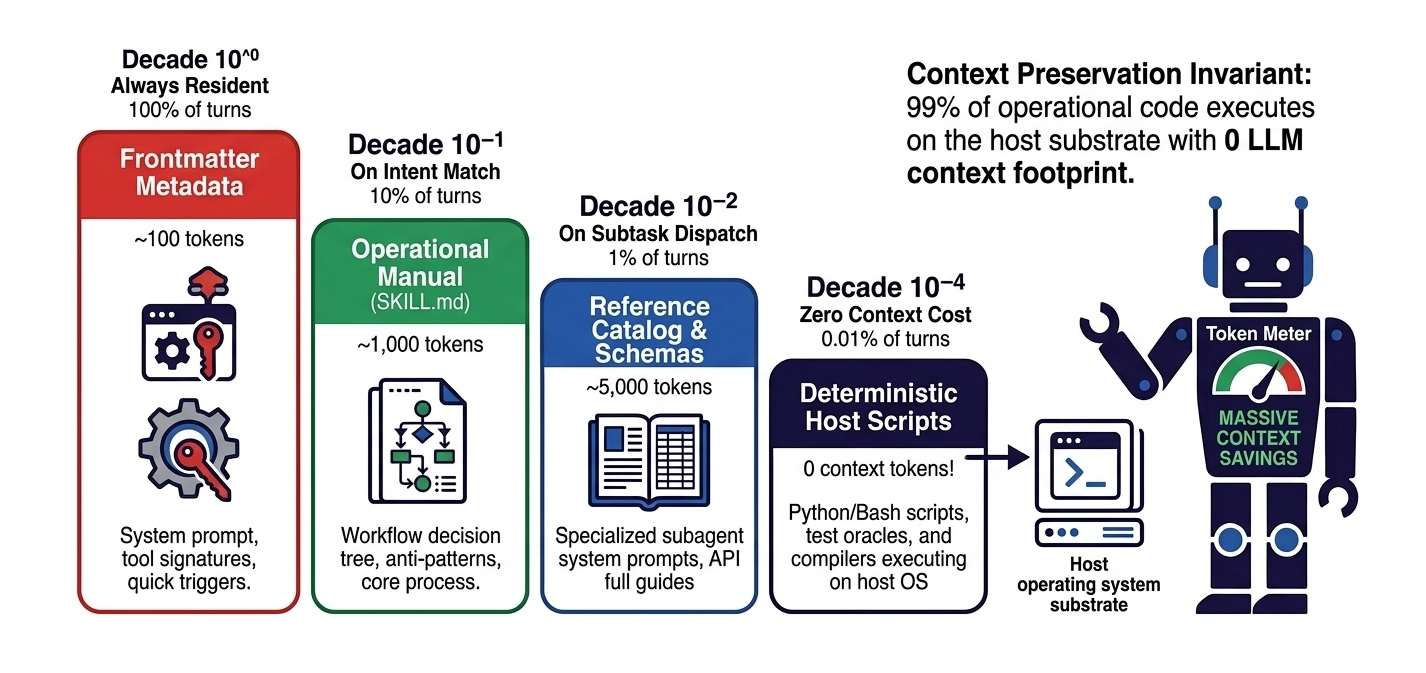
\includegraphics[width=\linewidth,height=8.0cm,keepaspectratio]{figures/fig-ch0-skills-diagram.jpg}
    \end{minipage}
    \tcblower
    \begin{minipage}[t][2.0cm][t]{\linewidth}
      \pdgrotesk\scriptsize
      \textbf{\color{pderror!90!black} Artifact \& Limitation Audit:}\\
      \begin{itemize}[leftmargin=9pt,itemsep=0pt,topsep=0.5pt,parsep=0pt]
        \item Raster diagram suffers from non-vector text pixelation at standard book scale
        \item Token counts (~100, ~1,000, ~5,000) blur when resized to two-page spread width
        \item Robot token meter icon and decade pill borders show compression ringing
      \end{itemize}
    \end{minipage}
  \end{tcolorbox}
\end{minipage}\hfill
\begin{minipage}[t]{0.492\linewidth}
  \begin{tcolorbox}[
    colback=pdcobalt!3,colframe=pdcobalt!85!black,arc=1.5pt,
    boxrule=0.7pt,top=1.5pt,bottom=1.5pt,left=4pt,right=4pt,
    title={\pdgrotesk\footnotesize\bfseries \color{white} B. Authoritative Native Vector Replacement \hfill \texttt{.tex / TikZ / PGF}}
  ]
    \begin{minipage}[c][8.3cm][c]{\linewidth}
      \centering
      \sbox{\pdfigbox}{% fig-ch0-progressive-skills.tex
% Progressive Disclosure of Skills Across Logarithmic Decades
% 100% native vector Swiss TikZ spatial replica of the AI-generated diagram prototype.

% pd-robot-glyphs.tex
% Authentic vector robot glyphs and system iconography for Port Daddy architectural figures.
% Provides 100% vector replacements matching the AI-generated diagram prototypes.

\ifdefined\pdrobotglyphsloaded\else
\def\pdrobotglyphsloaded{1}

% -----------------------------------------------------------------------------
% 1. Standard Standing Agent Robot (Base Model)
% Args: shift (x,y), color, scale
% -----------------------------------------------------------------------------
\newcommand{\pdrobotbase}[3][1.0]{%
  \begin{scope}[shift={#2},scale=#1]
    % Head
    \draw[fill=#3!85, draw=#3!95!black, line width=0.6pt, rounded corners=2pt] (-0.28, 0.22) rectangle (0.28, 0.58);
    % Dual Antennae
    \draw[line width=0.65pt, draw=#3!95!black] (-0.12, 0.58) -- (-0.16, 0.72);
    \draw[line width=0.65pt, draw=#3!95!black] (0.12, 0.58) -- (0.16, 0.72);
    \fill[pdamber!90!orange] (-0.16, 0.72) circle (0.038);
    \fill[pdamber!90!orange] (0.16, 0.72) circle (0.038);
    % Screen / Visor
    \draw[fill=hhink!90, draw=none, rounded corners=1.2pt] (-0.22, 0.28) rectangle (0.22, 0.52);
    % Eyes
    \fill[pdteal!35!white] (-0.11, 0.40) circle (0.04);
    \fill[pdteal!35!white] (0.11, 0.40) circle (0.04);
    % Mouth bar
    \draw[pdteal!35!white, line width=0.4pt] (-0.07, 0.33) -- (0.07, 0.33);
    % Ear bolts
    \draw[fill=pdslate!60, draw=#3!95!black, line width=0.4pt] (-0.32, 0.35) rectangle (-0.28, 0.45);
    \draw[fill=pdslate!60, draw=#3!95!black, line width=0.4pt] (0.28, 0.35) rectangle (0.32, 0.45);
    % Neck
    \draw[fill=pdslate!70, draw=#3!95!black, line width=0.4pt] (-0.08, 0.16) rectangle (0.08, 0.22);
    % Body / Torso
    \draw[fill=#3!85, draw=#3!95!black, line width=0.6pt, rounded corners=2pt] (-0.32, -0.28) rectangle (0.32, 0.16);
    % Chest panel
    \draw[fill=pdpage, draw=#3!70!black, line width=0.35pt, rounded corners=1pt] (-0.22, -0.12) rectangle (0.22, 0.10);
    \fill[pdhealth] (-0.13, -0.01) circle (0.03);
    \fill[pdamber] (0.0, -0.01) circle (0.03);
    \fill[pderror] (0.13, -0.01) circle (0.03);
    % Arms
    \draw[fill=#3!75, draw=#3!95!black, line width=0.45pt, rounded corners=1.2pt] (-0.44, -0.20) rectangle (-0.32, 0.10);
    \draw[fill=#3!75, draw=#3!95!black, line width=0.45pt, rounded corners=1.2pt] (0.32, -0.20) rectangle (0.44, 0.10);
    % Legs & Feet
    \draw[fill=pdslate!80, draw=#3!95!black, line width=0.45pt] (-0.24, -0.46) rectangle (-0.09, -0.28);
    \draw[fill=pdslate!80, draw=#3!95!black, line width=0.45pt] (0.09, -0.46) rectangle (0.24, -0.28);
    \draw[fill=pdslate!90!black, draw=#3!95!black, line width=0.45pt, rounded corners=1pt] (-0.28, -0.52) rectangle (-0.05, -0.44);
    \draw[fill=pdslate!90!black, draw=#3!95!black, line width=0.45pt, rounded corners=1pt] (0.05, -0.52) rectangle (0.28, -0.44);
  \end{scope}
}

% -----------------------------------------------------------------------------
% 2. Robot Holding Voting / Lease Token Tablet
% -----------------------------------------------------------------------------
\newcommand{\pdrobottoken}[3][1.0]{%
  \begin{scope}[shift={#2},scale=#1]
    % Head
    \draw[fill=#3!85, draw=#3!95!black, line width=0.6pt, rounded corners=2pt] (-0.28, 0.22) rectangle (0.28, 0.58);
    % Antenna
    \draw[line width=0.65pt, draw=#3!95!black] (0, 0.58) -- (0, 0.73);
    \fill[pdamber!90!orange] (0, 0.73) circle (0.04);
    % Screen / Visor
    \draw[fill=hhink!90, draw=none, rounded corners=1.2pt] (-0.22, 0.28) rectangle (0.22, 0.52);
    \fill[pdteal!35!white] (-0.11, 0.40) circle (0.04);
    \fill[pdteal!35!white] (0.11, 0.40) circle (0.04);
    \draw[pdteal!35!white, line width=0.4pt] (-0.07, 0.33) -- (0.07, 0.33);
    % Neck
    \draw[fill=pdslate!70, draw=#3!95!black, line width=0.4pt] (-0.08, 0.16) rectangle (0.08, 0.22);
    % Body
    \draw[fill=#3!85, draw=#3!95!black, line width=0.6pt, rounded corners=2pt] (-0.32, -0.28) rectangle (0.32, 0.16);
    % Legs & Feet
    \draw[fill=pdslate!80, draw=#3!95!black, line width=0.45pt] (-0.24, -0.46) rectangle (-0.09, -0.28);
    \draw[fill=pdslate!80, draw=#3!95!black, line width=0.45pt] (0.09, -0.46) rectangle (0.24, -0.28);
    \draw[fill=pdslate!90!black, draw=#3!95!black, line width=0.45pt, rounded corners=1pt] (-0.28, -0.52) rectangle (-0.05, -0.44);
    \draw[fill=pdslate!90!black, draw=#3!95!black, line width=0.45pt, rounded corners=1pt] (0.05, -0.52) rectangle (0.28, -0.44);
    % Arms holding tablet
    \draw[fill=#3!75, draw=#3!95!black, line width=0.45pt] (-0.42, -0.08) -- (-0.22, 0.05) -- (-0.18, 0.0) -- (-0.35, -0.13) -- cycle;
    \draw[fill=#3!75, draw=#3!95!black, line width=0.45pt] (0.42, -0.08) -- (0.22, 0.05) -- (0.18, 0.0) -- (0.35, -0.13) -- cycle;
    % Tablet
    \draw[fill=pdpage, draw=pdcobalt, line width=0.55pt, rounded corners=1.2pt] (-0.24, -0.18) rectangle (0.24, 0.18);
    \node[font=\fontsize{3.8}{4.5}\selectfont\bfseries\color{pdcobalt}] at (0, 0.06) {VOTING};
    \node[font=\fontsize{3.5}{4.2}\selectfont\bfseries\color{hhink}] at (0, -0.06) {TOKEN};
  \end{scope}
}

% -----------------------------------------------------------------------------
% 3. Robot at Laptop / Deliberation
% -----------------------------------------------------------------------------
\newcommand{\pdrobotlaptop}[3][1.0]{%
  \begin{scope}[shift={#2},scale=#1]
    % Head (Tilted slightly forward)
    \draw[fill=#3!85, draw=#3!95!black, line width=0.6pt, rounded corners=2pt] (-0.26, 0.22) rectangle (0.26, 0.56);
    % Dual Antennae
    \draw[line width=0.65pt, draw=#3!95!black] (-0.10, 0.56) -- (-0.14, 0.70);
    \draw[line width=0.65pt, draw=#3!95!black] (0.10, 0.56) -- (0.14, 0.70);
    \fill[pdteal] (-0.14, 0.70) circle (0.038);
    \fill[pdteal] (0.14, 0.70) circle (0.038);
    % Visor
    \draw[fill=hhink!90, draw=none, rounded corners=1.2pt] (-0.20, 0.28) rectangle (0.20, 0.50);
    \fill[pdteal!40!white] (-0.10, 0.38) circle (0.038);
    \fill[pdteal!40!white] (0.10, 0.38) circle (0.038);
    % Body
    \draw[fill=#3!85, draw=#3!95!black, line width=0.6pt, rounded corners=2pt] (-0.30, -0.26) rectangle (0.30, 0.18);
    % Legs (Seated)
    \draw[fill=pdslate!80, draw=#3!95!black, line width=0.45pt] (-0.25, -0.38) rectangle (0.25, -0.26);
    % Desk surface
    \draw[line width=1.0pt, pdslate!80!black] (-0.6, -0.38) -- (0.7, -0.38);
    % Laptop Base
    \draw[fill=pdslate!40, draw=pdslate!90!black, line width=0.45pt] (-0.05, -0.38) -- (0.50, -0.38) -- (0.46, -0.33) -- (-0.02, -0.33) -- cycle;
    % Laptop Screen
    \draw[fill=pdcobalt!90!black, draw=pdslate!90!black, line width=0.5pt, rounded corners=1pt] (0.42, -0.33) -- (0.52, 0.05) -- (0.15, 0.05) -- (0.08, -0.33) -- cycle;
    % Glowing Screen Text
    \draw[pdteal!50!white, line width=0.4pt] (0.18, -0.03) -- (0.42, -0.03);
    \draw[pdteal!50!white, line width=0.4pt] (0.16, -0.12) -- (0.38, -0.12);
    \draw[pdteal!50!white, line width=0.4pt] (0.14, -0.21) -- (0.34, -0.21);
    % Arms on keyboard
    \draw[fill=#3!75, draw=#3!95!black, line width=0.45pt] (-0.22, 0.05) to[out=-20,in=160] (0.12, -0.30) -- (0.18, -0.33) -- (-0.18, -0.05) -- cycle;
  \end{scope}
}

% -----------------------------------------------------------------------------
% 4. Red-and-White Disablement Barrier
% -----------------------------------------------------------------------------
\newcommand{\pdbarrierline}[4]{% (x1, y1) to (x2, y2)
  \draw[line width=4.5pt, white] (#1,#2) -- (#3,#4);
  \draw[line width=4.5pt, pderror, dashed, dash pattern=on 6pt off 6pt] (#1,#2) -- (#3,#4);
  \draw[line width=0.6pt, pderror!80!black] (#1,#2) -- (#3,#4);
}

% -----------------------------------------------------------------------------
% 5. Vector Iconography Definitions
% -----------------------------------------------------------------------------
% Crossed Tools (Wrench + Screwdriver)
\newcommand{\pdicontools}[2][1.0]{%
  \begin{scope}[shift={#2},scale=#1]
    \draw[line width=1.4pt, pdslate!80!black, line cap=round] (-0.25,-0.25) -- (0.25,0.25);
    \draw[line width=1.4pt, pdrust!90!black, line cap=round] (-0.25,0.25) -- (0.25,-0.25);
    \draw[fill=pdslate!90!black, line width=0.4pt] (0.18,0.18) circle (0.10);
    \fill[white] (0.20,0.20) circle (0.04);
    \draw[fill=pdrust!90!black, line width=0.4pt] (0.20,-0.22) rectangle (0.26,-0.16);
  \end{scope}
}

% Git Branch
\newcommand{\pdicongit}[2][1.0]{%
  \begin{scope}[shift={#2},scale=#1]
    \draw[line width=1.1pt, pdteal!90!black] (0,-0.32) -- (0,0.32);
    \draw[line width=1.1pt, pdteal!90!black] (0,-0.08) to[out=45,in=180] (0.24,0.16);
    \fill[pdteal!90!black] (0,-0.24) circle (0.06);
    \fill[pdteal!90!black] (0,0.24) circle (0.06);
    \fill[pdteal!90!black] (0.24,0.16) circle (0.06);
  \end{scope}
}

% Network Globe
\newcommand{\pdiconglobe}[2][1.0]{%
  \begin{scope}[shift={#2},scale=#1]
    \draw[line width=0.7pt, pdcobalt!85!black] (0,0) circle (0.28);
    \draw[line width=0.5pt, pdcobalt!70] (0,0) ellipse (0.13 and 0.28);
    \draw[line width=0.5pt, pdcobalt!70] (-0.28,0) -- (0.28,0);
    \draw[line width=0.5pt, pdcobalt!70] (-0.24,0.14) -- (0.24,0.14);
    \draw[line width=0.5pt, pdcobalt!70] (-0.24,-0.14) -- (0.24,-0.14);
  \end{scope}
}

% Host OS Gear / Process
\newcommand{\pdicongear}[2][1.0]{%
  \begin{scope}[shift={#2},scale=#1]
    \fill[pdslate!75!black] (0,0) circle (0.22);
    \foreach \a in {0,45,90,135,180,225,270,315} {
      \fill[pdslate!75!black] (\a:0.26) circle (0.055);
    }
    \fill[white] (0,0) circle (0.09);
  \end{scope}
}

% Stopwatch / Timer
\newcommand{\pdicontimer}[2][1.0]{%
  \begin{scope}[shift={#2},scale=#1]
    \draw[line width=0.75pt, pdamber!90!black] (0,0) circle (0.25);
    \draw[line width=0.8pt, pdamber!90!black] (0,0.25) -- (0,0.33);
    \draw[line width=1.0pt, pdamber!90!black] (-0.06,0.33) -- (0.06,0.33);
    \draw[line width=0.75pt, pdamber!90!black] (0,0) -- (0,0.14);
    \draw[line width=0.75pt, pdamber!90!black] (0,0) -- (0.11,0.05);
    \fill[pdamber!90!black] (0,0) circle (0.035);
  \end{scope}
}

% Hardware Crash / Lightning Burst
\newcommand{\pdiconcrash}[2][1.0]{%
  \begin{scope}[shift={#2},scale=#1]
    \fill[pderror!90!black] (0.06,0.32) -- (-0.12,0.04) -- (-0.02,0.04) -- (-0.14,-0.32) -- (0.12,-0.02) -- (0.02,-0.02) -- cycle;
  \end{scope}
}

% Shield with Checkmark
\newcommand{\pdiconshieldcheck}[2][1.0]{%
  \begin{scope}[shift={#2},scale=#1]
    \fill[pdcobalt!90!black] (0,0.32) -- (0.26,0.20) to[out=-70,in=45] (0,-0.32) to[out=135,in=-110] (-0.26,0.20) -- cycle;
    \draw[line width=1.1pt, white, line cap=round, line join=round] (-0.11,-0.02) -- (-0.03,-0.12) -- (0.13,0.10);
  \end{scope}
}

% Padlock
\newcommand{\pdiconlock}[2][1.0]{%
  \begin{scope}[shift={#2},scale=#1]
    % Shackle
    \draw[line width=0.9pt, pdslate!80!black] (-0.12,0.05) -- (-0.12,0.18) arc (180:0:0.12) -- (0.12,0.05);
    % Body
    \draw[fill=pderror!85!black, draw=pderror!95!black, line width=0.5pt, rounded corners=1pt] (-0.18,-0.20) rectangle (0.18,0.06);
    % Keyhole
    \fill[white] (0,-0.04) circle (0.035);
    \draw[line width=0.6pt, white] (0,-0.04) -- (0,-0.13);
  \end{scope}
}

% Speedometer / Spend Cap
\newcommand{\pdiconspeedometer}[2][1.0]{%
  \begin{scope}[shift={#2},scale=#1]
    \draw[line width=1.0pt, pdteal!90!black] (-0.28,-0.04) arc (180:40:0.28);
    \draw[line width=1.0pt, pderror] (40:0.28) arc (40:0:0.28);
    \draw[line width=0.8pt, hhink, line cap=round] (0,-0.04) -- (0.12,0.14);
    \fill[hhink] (0,-0.04) circle (0.05);
  \end{scope}
}

% Sparkle Broom / Hygiene Wand
\newcommand{\pdiconbroom}[2][1.0]{%
  \begin{scope}[shift={#2},scale=#1]
    \draw[line width=1.2pt, pdteal!90!black, line cap=round] (-0.2,-0.2) -- (0.15,0.15);
    % Sparkles
    \fill[pdamber!90!orange] (0.22,0.22) circle (0.04);
    \fill[pdteal] (0.05,0.26) circle (0.03);
    \fill[pdteal] (0.26,0.05) circle (0.03);
  \end{scope}
}

% Host Terminal Substrate
\newcommand{\pdiconterminal}[2][1.0]{%
  \begin{scope}[shift={#2},scale=#1]
    \draw[fill=hhink!95, draw=pdslate!80, line width=0.6pt, rounded corners=1.5pt] (-0.35,-0.25) rectangle (0.35,0.25);
    \draw[fill=pderror] (-0.26,0.18) circle (0.025);
    \fill[pdamber] (-0.18,0.18) circle (0.025);
    \fill[pdhealth] (-0.10,0.18) circle (0.025);
    \node[font=\fontsize{4.5}{5}\selectfont\ttfamily\color{pdhealth}] at (0,-0.05) {>\_};
  \end{scope}
}

% Coins Stack
\newcommand{\pdiconcoins}[2][1.0]{%
  \begin{scope}[shift={#2},scale=#1]
    \foreach \y in {-0.24, -0.12, 0.0, 0.12} {
      \draw[fill=pdamber!80!orange, draw=pdamber!95!black, line width=0.45pt] (0,\y) ellipse (0.24 and 0.07);
    }
  \end{scope}
}

% Tall Coins Stack
\newcommand{\pdiconcoinstall}[2][1.0]{%
  \begin{scope}[shift={#2},scale=#1]
    \foreach \y in {-0.30, -0.18, -0.06, 0.06, 0.18, 0.30} {
      \draw[fill=pdamber!80!orange, draw=pdamber!95!black, line width=0.45pt] (0,\y) ellipse (0.24 and 0.07);
    }
  \end{scope}
}

% Slashed Coins (Stake Slashed)
\newcommand{\pdiconcoinslashed}[2][1.0]{%
  \begin{scope}[shift={#2},scale=#1]
    \foreach \y in {-0.20, -0.08, 0.04, 0.16} {
      \draw[fill=pdamber!70!white, draw=pdamber!80!black, line width=0.45pt] (0,\y) ellipse (0.22 and 0.065);
    }
    \draw[line width=1.5pt, pderror, line cap=round] (-0.26,-0.24) -- (0.26,0.24);
  \end{scope}
}

% Magnifying Glass (Audit Inspection)
\newcommand{\pdiconmagnifier}[2][1.0]{%
  \begin{scope}[shift={#2},scale=#1]
    \draw[line width=0.9pt, pdteal!90!black] (0,0.06) circle (0.16);
    \draw[line width=1.4pt, pdteal!90!black, line cap=round] (0.12,-0.06) -- (0.26,-0.20);
    \fill[white] (-0.04,0.10) circle (0.04);
  \end{scope}
}

% Arbitration Gavel & Scales of Justice
\newcommand{\pdiconarbitration}[2][1.0]{%
  \begin{scope}[shift={#2},scale=#1]
    % Central post
    \draw[line width=0.8pt, pdrust!90!black] (0.15,-0.20) -- (0.15,0.22);
    \draw[line width=0.8pt, pdrust!90!black] (-0.05,0.18) -- (0.35,0.18);
    \draw[line width=0.5pt, pdrust!80] (-0.05,0.18) -- (-0.12,0.02) -- (0.02,0.02) -- cycle;
    \draw[line width=0.5pt, pdrust!80] (0.35,0.18) -- (0.28,0.02) -- (0.42,0.02) -- cycle;
    % Gavel
    \draw[line width=1.4pt, pdrust!95!black, line cap=round] (-0.30,-0.18) -- (-0.10,0.05);
    \draw[fill=pdrust!90!black, draw=pdrust!95!black, line width=0.5pt, rounded corners=1pt] (-0.22,0.0) -- (-0.12,0.12) -- (-0.02,0.04) -- (-0.12,-0.08) -- cycle;
  \end{scope}
}

% Cash Bill / Liquidated Damages
\newcommand{\pdiconcash}[2][1.0]{%
  \begin{scope}[shift={#2},scale=#1]
    \draw[fill=white, draw=pdslate!90!black, line width=0.6pt, rounded corners=1.5pt] (-0.35,-0.20) rectangle (0.35,0.20);
    \draw[line width=0.5pt, pdteal!80!black] (-0.28,-0.14) rectangle (0.28,0.14);
    \fill[pdteal!90!black] (0,0) circle (0.08);
    \fill[pdteal!90!black] (-0.22,0) circle (0.035);
    \fill[pdteal!90!black] (0.22,0) circle (0.035);
  \end{scope}
}

% Group of People / Remedy
\newcommand{\pdicongrouppeople}[2][1.0]{%
  \begin{scope}[shift={#2},scale=#1]
    % Center person
    \fill[hhink] (0,0.12) circle (0.09);
    \fill[hhink] (-0.15,-0.20) to[out=70,in=180] (0,-0.02) to[out=0,in=110] (0.15,-0.20) -- cycle;
    % Left person
    \fill[hhgray!90!black] (-0.22,0.06) circle (0.075);
    \fill[hhgray!90!black] (-0.34,-0.20) to[out=70,in=180] (-0.22,-0.06) to[out=0,in=110] (-0.10,-0.20) -- cycle;
    % Right person
    \fill[hhgray!90!black] (0.22,0.06) circle (0.075);
    \fill[hhgray!90!black] (0.10,-0.20) to[out=70,in=180] (0.22,-0.06) to[out=0,in=110] (0.34,-0.20) -- cycle;
  \end{scope}
}

% Database Cylinder
\newcommand{\pdicondatabase}[2][1.0]{%
  \begin{scope}[shift={#2},scale=#1]
    \draw[fill=pdslate!20, draw=pdslate!90!black, line width=0.6pt] (-0.25,-0.15) rectangle (0.25,0.15);
    \draw[fill=pdslate!30, draw=pdslate!90!black, line width=0.5pt] (0,0.15) ellipse (0.25 and 0.08);
    \draw[draw=pdslate!90!black, line width=0.5pt] (-0.25,0) arc (180:360:0.25 and 0.08);
    \draw[draw=pdslate!90!black, line width=0.5pt] (-0.25,-0.15) arc (180:360:0.25 and 0.08);
  \end{scope}
}

% Signed Document / Witness Receipts
\newcommand{\pdicondocument}[2][1.0]{%
  \begin{scope}[shift={#2},scale=#1]
    \draw[fill=white, draw=pdslate!90!black, line width=0.55pt] (-0.18,-0.24) -- (0.10,-0.24) -- (0.18,-0.16) -- (0.18,0.24) -- (-0.18,0.24) -- cycle;
    \draw[draw=pdslate!80, line width=0.45pt] (0.10,-0.24) -- (0.10,-0.16) -- (0.18,-0.16);
    \draw[pdslate!70, line width=0.4pt] (-0.12,0.16) -- (0.12,0.16);
    \draw[pdslate!70, line width=0.4pt] (-0.12,0.08) -- (0.12,0.08);
    \draw[pdslate!70, line width=0.4pt] (-0.12,0.00) -- (0.06,0.00);
    % Feather / quill
    \draw[line width=0.7pt, pdcobalt!80!black] (0.08,-0.12) to[out=45,in=-45] (0.24,0.06);
  \end{scope}
}

% Merkle Inclusion Proof Tree
\newcommand{\pdiconmerkle}[2][1.0]{%
  \begin{scope}[shift={#2},scale=#1]
    % Root
    \draw[line width=0.5pt, pdslate!80] (0,0.20) -- (-0.16,0.04);
    \draw[line width=0.5pt, pdslate!80] (0,0.20) -- (0.16,0.04);
    \draw[line width=0.5pt, pdslate!80] (-0.16,0.04) -- (-0.24,-0.14);
    \draw[line width=0.5pt, pdslate!80] (-0.16,0.04) -- (-0.08,-0.14);
    \draw[line width=0.5pt, pdslate!80] (0.16,0.04) -- (0.08,-0.14);
    \draw[line width=0.5pt, pdslate!80] (0.16,0.04) -- (0.24,-0.14);
    \draw[fill=white, draw=pdslate!90!black, line width=0.4pt] (-0.05,0.16) rectangle (0.05,0.24);
    \draw[fill=white, draw=pdslate!90!black, line width=0.4pt] (-0.20,0.0) rectangle (-0.12,0.08);
    \draw[fill=white, draw=pdslate!90!black, line width=0.4pt] (0.12,0.0) rectangle (0.20,0.08);
    \draw[fill=pdteal!80!white, draw=pdteal!95!black, line width=0.5pt] (-0.28,-0.18) rectangle (-0.20,-0.10);
    \draw[fill=white, draw=pdslate!90!black, line width=0.4pt] (-0.12,-0.18) rectangle (-0.04,-0.10);
    \draw[fill=white, draw=pdslate!90!black, line width=0.4pt] (0.04,-0.18) rectangle (0.12,-0.10);
    \draw[fill=white, draw=pdslate!90!black, line width=0.4pt] (0.20,-0.18) rectangle (0.28,-0.10);
  \end{scope}
}

% Key (Cryptographic Key / Capability Key)
\newcommand{\pdiconkey}[2][1.0]{%
  \begin{scope}[shift={#2},scale=#1]
    \draw[line width=0.8pt, pdamber!95!black] (0, 0.12) circle (0.14);
    \fill[white] (0, 0.12) circle (0.06);
    \draw[line width=0.85pt, pdamber!95!black] (0, -0.02) -- (0, -0.26);
    \draw[line width=0.7pt, pdamber!95!black] (0, -0.14) -- (0.10, -0.14);
    \draw[line width=0.7pt, pdamber!95!black] (0, -0.22) -- (0.08, -0.22);
  \end{scope}
}

\def\pdiconclock{\pdicontimer}
\def\pdiconlightning{\pdiconcrash}

\fi

\pdfigurehue{pdcobalt}%
\begin{tikzpicture}[pd figure,x=1cm,y=1cm]
  \tikzset{
    decbox1/.style={draw=pderror!90!black,line width=0.9pt,fill=white,rounded corners=4pt},
    decbox2/.style={draw=pdteal!85!black,line width=0.9pt,fill=white,rounded corners=4pt},
    decbox3/.style={draw=pdcobalt!90!black,line width=0.9pt,fill=white,rounded corners=4pt},
    decbox4/.style={draw=pdslate!90!black,line width=0.9pt,fill=white,rounded corners=4pt}
  }

  % =========================================================================
  % TOP RIGHT: CONTEXT PRESERVATION INVARIANT PROSE (Exact match to prototype)
  % =========================================================================
  \node[anchor=north west,text width=4.3cm,align=left] at (8.3, 7.3) {%
    {\fontsize{7.5}{9.2}\selectfont\bfseries\color{hhink} Context Preservation Invariant:}\\[2pt]
    {\fontsize{6.8}{8.2}\selectfont\color{hhink}%
    99\% of operational code executes on the host substrate with \textbf{0 LLM context footprint}.}%
  };

  % =========================================================================
  % FOUR PROGRESSIVE DECADE CARDS (x in [0.2, 9.35])
  % =========================================================================

  % --- CARD 1: Decade 10^0 (Frontmatter Metadata) ---
  \begin{scope}[shift={(0.2, 0.4)}]
    % Subheader above card
    \node[anchor=south,font=\fontsize{6.5}{7.8}\selectfont\bfseries\color{hhink},align=center] at (1.05, 5.55) {%
      Decade $\mathbf{10^0}$\\Always Resident\\{\fontsize{5.5}{6.5}\selectfont 100\% of turns}%
    };
    % Card Body (Red border)
    \draw[decbox1] (0, 0) rectangle (2.1, 5.5);
    % Top Header Pill (Red)
    \draw[fill=pderror!90!black,draw=none,rounded corners=3pt] (0.05, 4.50) rectangle (2.05, 5.45);
    \node[font=\fontsize{7.2}{8.5}\selectfont\bfseries\color{white},align=center] at (1.05, 4.95) {%
      Frontmatter\\Metadata%
    };
    % Token pill
    \node[draw=pderror!70,fill=pderror!8,line width=0.5pt,rounded corners=2pt,font=\fontsize{6.2}{7.4}\selectfont\bfseries\color{pderror!90!black}] at (1.05, 4.05) {%
      $\sim$100 tokens%
    };
    % Icons: Upper Browser with Gear/Key, Lower Gear with Key
    \begin{scope}[shift={(1.05, 2.85)}]
      % Upper browser window with upload arrow
      \draw[fill=hhpaper,draw=pdslate!70,line width=0.5pt,rounded corners=1.5pt] (-0.45, 0.25) rectangle (0.45, 0.70);
      \fill[pdslate!60] (-0.35, 0.60) circle (0.035);
      \fill[pdslate!60] (-0.25, 0.60) circle (0.035);
      \fill[pdslate!60] (-0.15, 0.60) circle (0.035);
      \pdicongear[0.35]{(-0.2, 0.40)}
      \pdiconkey[0.35]{(0.2, 0.40)}
      \draw[pd arrow,line width=0.8pt,pderror] (0, 0.70) -- (0, 0.90);

      % Lower large gear with diagonal key
      \pdicongear[0.75]{(0.0, -0.45)}
      \begin{scope}[shift={(0.0, -0.45)},rotate=-45]
        \pdiconkey[0.65]{(0, 0)}
      \end{scope}
    \end{scope}
    % Description
    \node[anchor=north,font=\fontsize{6.0}{7.2}\selectfont\color{hhink},align=center,text width=2.0cm] at (1.05, 1.35) {%
      System prompt,\\tool signatures,\\quick triggers.%
    };
  \end{scope}

  % --- CARD 2: Decade 10^-1 (Operational Manual) ---
  \begin{scope}[shift={(2.55, 0.4)}]
    % Subheader above card
    \node[anchor=south,font=\fontsize{6.5}{7.8}\selectfont\bfseries\color{hhink},align=center] at (1.05, 5.05) {%
      Decade $\mathbf{10^{-1}}$\\On Intent Match\\{\fontsize{5.5}{6.5}\selectfont 10\% of turns}%
    };
    % Card Body (Green border)
    \draw[decbox2] (0, 0) rectangle (2.1, 5.0);
    % Top Header Pill (Green)
    \draw[fill=pdteal!85!black,draw=none,rounded corners=3pt] (0.05, 4.05) rectangle (2.05, 4.95);
    \node[font=\fontsize{7.0}{8.3}\selectfont\bfseries\color{white},align=center] at (1.05, 4.50) {%
      Operational\\Manual {\fontsize{5.2}{6.2}\selectfont(SKILL.md)}%
    };
    % Token pill
    \node[draw=pdteal!80,fill=pdteal!8,line width=0.5pt,rounded corners=2pt,font=\fontsize{6.2}{7.4}\selectfont\bfseries\color{pdteal!90!black}] at (1.05, 3.60) {%
      $\sim$1,000 tokens%
    };
    % Flowchart Document Icon
    \begin{scope}[shift={(1.05, 2.55)}]
      \draw[fill=hhpaper,draw=pdslate!80,line width=0.6pt,rounded corners=1.5pt] (-0.50, -0.65) rectangle (0.50, 0.65);
      % 3 header dots
      \fill[pdslate!60] (-0.35, 0.52) circle (0.035);
      \fill[pdslate!60] (-0.22, 0.52) circle (0.035);
      \fill[pdslate!60] (-0.09, 0.52) circle (0.035);
      % Start circle
      \draw[fill=pdteal!30,draw=pdteal,line width=0.4pt] (0, 0.35) circle (0.08);
      \draw[pd arrow,line width=0.4pt,pdteal] (0, 0.27) -- (0, 0.14);
      % Decision Diamond
      \draw[fill=pdteal!20,draw=pdteal,line width=0.4pt] (0, 0.14) -- (0.18, 0) -- (0, -0.14) -- (-0.18, 0) -- cycle;
      % Action boxes
      \draw[pd arrow,line width=0.4pt,pdteal] (-0.18, 0) -- (-0.30, 0) -- (-0.30, -0.30);
      \draw[pd arrow,line width=0.4pt,pdteal] (0.18, 0) -- (0.30, 0) -- (0.30, -0.30);
      \draw[fill=pdteal!40,draw=pdteal,line width=0.4pt] (-0.40, -0.46) rectangle (-0.20, -0.30);
      \draw[fill=pdteal!40,draw=pdteal,line width=0.4pt] (0.20, -0.46) rectangle (0.40, -0.30);
      % Feedback loop
      \draw[line width=0.35pt,pdteal] (-0.30, -0.46) -- (-0.30, -0.56) -- (0.30, -0.56) -- (0.30, -0.46);
    \end{scope}
    % Description
    \node[anchor=north,font=\fontsize{6.0}{7.2}\selectfont\color{hhink},align=center,text width=2.0cm] at (1.05, 1.35) {%
      Workflow decision\\tree, anti-patterns,\\core process.%
    };
  \end{scope}

  % --- CARD 3: Decade 10^-2 (Reference Catalog & Schemas) ---
  \begin{scope}[shift={(4.9, 0.4)}]
    % Subheader above card
    \node[anchor=south,font=\fontsize{6.5}{7.8}\selectfont\bfseries\color{hhink},align=center] at (1.05, 4.55) {%
      Decade $\mathbf{10^{-2}}$\\On Subtask Dispatch\\{\fontsize{5.5}{6.5}\selectfont 1\% of turns}%
    };
    % Card Body (Blue border)
    \draw[decbox3] (0, 0) rectangle (2.1, 4.65);
    % Top Header Pill (Vibrant Cobalt)
    \draw[fill=pdcobalt,draw=none,rounded corners=3pt] (0.05, 3.55) rectangle (2.05, 4.60);
    \node[text=white,font=\fontsize{7.0}{8.3}\selectfont\bfseries,align=center] at (1.05, 4.07) {%
      Reference\\Catalog \& Schemas%
    };
    % Token pill
    \node[draw=pdcobalt!80,fill=pdcobalt!8,line width=0.5pt,rounded corners=2pt,font=\fontsize{6.2}{7.4}\selectfont\bfseries\color{pdcobalt}] at (1.05, 3.15) {%
      $\sim$5,000 tokens%
    };
    % Open Book Icon
    \begin{scope}[shift={(1.05, 2.30)}]
      \draw[fill=hhpaper,draw=pdcobalt!90,line width=0.7pt,rounded corners=1pt] (-0.55, -0.45) rectangle (0.55, 0.45);
      \draw[line width=0.6pt,pdcobalt!90] (0, -0.45) -- (0, 0.45);
      % Left page: square block and lines
      \draw[fill=pdcobalt!30,draw=none] (-0.45, 0.12) rectangle (-0.22, 0.35);
      \draw[line width=0.4pt,pdcobalt!70] (-0.45, -0.05) -- (-0.1, -0.05);
      \draw[line width=0.4pt,pdcobalt!70] (-0.45, -0.18) -- (-0.1, -0.18);
      \draw[line width=0.4pt,pdcobalt!70] (-0.45, -0.32) -- (-0.2, -0.32);
      % Right page: table grid
      \draw[line width=0.4pt,pdcobalt!70] (0.1, 0.32) -- (0.45, 0.32);
      \draw[line width=0.4pt,pdcobalt!70] (0.1, 0.16) -- (0.45, 0.16);
      \draw[line width=0.4pt,pdcobalt!70] (0.1, 0.0) -- (0.45, 0.0);
      \draw[line width=0.4pt,pdcobalt!70] (0.1, -0.16) -- (0.45, -0.16);
      \draw[line width=0.4pt,pdcobalt!70] (0.1, -0.32) -- (0.45, -0.32);
      \draw[line width=0.4pt,pdcobalt!70] (0.27, -0.38) -- (0.27, 0.38);
    \end{scope}
    % Description
    \node[anchor=north,font=\fontsize{6.0}{7.2}\selectfont\color{hhink},align=center,text width=2.0cm] at (1.05, 1.45) {%
      Specialized subagent\\system prompts, API\\full guides%
    };
  \end{scope}

  % --- CARD 4: Decade 10^-4 (Deterministic Host Scripts) ---
  \begin{scope}[shift={(7.25, 0.4)}]
    % Subheader above card
    \node[anchor=south,font=\fontsize{6.5}{7.8}\selectfont\bfseries\color{hhink},align=center] at (1.05, 4.05) {%
      Decade $\mathbf{10^{-4}}$\\Zero Context Cost\\{\fontsize{5.5}{6.5}\selectfont 0.01\% of turns}%
    };
    % Card Body (Dark navy border)
    \draw[decbox4] (0, 0) rectangle (2.1, 4.0);
    % Top Header Pill (Dark Navy)
    \draw[fill=pdslate!90!black,draw=none,rounded corners=3pt] (0.05, 3.05) rectangle (2.05, 3.95);
    \node[text=white,font=\fontsize{7.0}{8.3}\selectfont\bfseries,align=center] at (1.05, 3.50) {%
      Deterministic\\Host Scripts%
    };
    % Token pill (Zero Context!)
    \node[draw=pdhealth!80!black,fill=pdhealth!12,line width=0.5pt,rounded corners=2pt,font=\fontsize{6.2}{7.4}\selectfont\bfseries\color{pdhealth!90!black}] at (1.05, 2.65) {%
      \textbf{0 context tokens!}%
    };
    % Description
    \node[anchor=north,font=\fontsize{5.2}{6.2}\selectfont\color{hhink},align=center,text width=2.0cm] at (1.05, 2.0) {%
      Python/Bash scripts,\\test oracles, and\\compilers executing\\on host OS%
    };
  \end{scope}

  % =========================================================================
  % RIGHT: COMPUTER TERMINAL AND BIG ROBOT WITH TOKEN METER
  % =========================================================================

  % Arrow from Card 4 to Host Terminal
  \draw[pd arrow,line width=1.3pt,hhink] (9.45, 2.3) -- (10.05, 2.3);

  % Host Terminal Station (x=10.65, y=2.3)
  \begin{scope}[shift={(10.65, 2.3)}]
    % Monitor
    \draw[fill=hhpaper,draw=pdslate!90!black,line width=0.9pt,rounded corners=2pt] (-0.50, -0.22) rectangle (0.50, 0.60);
    \draw[fill=pdslate!90!black,draw=none,rounded corners=1.5pt] (-0.44, -0.16) rectangle (0.44, 0.44);
    % 3 dots top bar
    \fill[pdslate!60] (-0.38, 0.52) circle (0.028);
    \fill[pdslate!60] (-0.29, 0.52) circle (0.028);
    \fill[pdslate!60] (-0.20, 0.52) circle (0.028);
    % Terminal prompt
    \node[font=\fontsize{7.5}{8.5}\selectfont\bfseries\color{white}] at (-0.1, 0.16) {\texttt{>\_}};

    % Base unit / keyboard underneath
    \draw[fill=hhpaper,draw=pdslate!90!black,line width=0.9pt,rounded corners=1.5pt] (-0.55, -0.60) rectangle (0.55, -0.32);
    \fill[pdslate!60] (-0.38, -0.46) circle (0.035);
    \fill[pdslate!60] (-0.24, -0.46) circle (0.035);
    \fill[pdslate!60] (-0.10, -0.46) circle (0.035);
    \draw[line width=0.9pt,pdslate!70] (0.12, -0.46) -- (0.40, -0.46);

    % Label below terminal
    \node[anchor=north,font=\fontsize{6.0}{7.2}\selectfont\bfseries\color{hhink},align=center] at (0, -0.72) {%
      Host\\operating system\\substrate%
    };
  \end{scope}

  % =========================================================================
  % BIG VECTOR ROBOT WITH INTEGRATED TOKEN METER (x=12.4, y=2.8)
  % =========================================================================
  \begin{scope}[shift={(12.4, 2.8)}]
    % Head: rounded rectangle with antennas, glowing eyes, mouth
    \draw[fill=pdcobalt!90!black,draw=pdcobalt!95!black,line width=1.1pt,rounded corners=3.5pt] (-0.60, 1.55) rectangle (0.60, 2.45);
    % Antennas with ball tips
    \draw[line width=1.1pt,pdcobalt!90!black] (-0.38, 2.45) -- (-0.38, 2.85);
    \fill[pdcobalt!90!black] (-0.38, 2.85) circle (0.09);
    \draw[line width=1.1pt,pdcobalt!90!black] (0.38, 2.45) -- (0.38, 2.85);
    \fill[pdcobalt!90!black] (0.38, 2.85) circle (0.09);
    % Ears / Bolts
    \fill[pdcobalt!70!black] (-0.72, 1.88) rectangle (-0.60, 2.12);
    \fill[pdcobalt!70!black] (0.60, 1.88) rectangle (0.72, 2.12);
    % Glowing Eyes
    \fill[white] (-0.28, 2.0) circle (0.10);
    \fill[white] (0.28, 2.0) circle (0.10);
    % Mouth line
    \draw[line width=1.4pt,white,line cap=round] (-0.28, 1.72) -- (0.28, 1.72);

    % Neck joint
    \fill[pdslate!60!black] (-0.20, 1.45) rectangle (0.20, 1.55);

    % Arms on hips (symmetric, clean, matching prototype)
    % Left Arm
    \fill[pdcobalt!70!black] (-0.80, 1.15) circle (0.13);
    \draw[line width=3.5pt,pdcobalt!90!black,line cap=round,line join=round] (-0.80, 1.15) -- (-1.15, 0.45) -- (-0.80, -0.15);
    \draw[line width=1.6pt,pdcobalt!95!black] (-0.80, -0.15) to[out=-135,in=90] (-0.95, -0.40);
    \draw[line width=1.6pt,pdcobalt!95!black] (-0.80, -0.15) to[out=-45,in=90] (-0.65, -0.40);

    % Right Arm
    \fill[pdcobalt!70!black] (0.80, 1.15) circle (0.13);
    \draw[line width=3.5pt,pdcobalt!90!black,line cap=round,line join=round] (0.80, 1.15) -- (1.15, 0.45) -- (0.80, -0.15);
    \draw[line width=1.6pt,pdcobalt!95!black] (0.80, -0.15) to[out=-45,in=90] (0.95, -0.40);
    \draw[line width=1.6pt,pdcobalt!95!black] (0.80, -0.15) to[out=-135,in=90] (0.65, -0.40);

    % TORSO: INTEGRAL TOKEN METER (Chest)
    \draw[fill=pdcobalt!95!black,draw=pdcobalt!95!black,line width=1.1pt,rounded corners=4.5pt] (-0.80, -0.90) rectangle (0.80, 1.45);

    % Token Meter Header
    \node[text=white,font=\fontsize{7.0}{8.2}\selectfont\bfseries] at (0, 1.22) {Token Meter};

    % Rainbow Gauge / Semi-Circle Arc
    \begin{scope}[shift={(0, 0.58)}]
      % Background white dial
      \fill[white] (-0.58, 0) arc (180:0:0.58) -- cycle;
      % Green section (left)
      \fill[pdhealth!90!black] (-0.58, 0) arc (180:90:0.58) -- (0, 0) -- cycle;
      % Red section (right)
      \fill[pderror!90!black] (0, 0) arc (90:0:0.58) -- (0, 0) -- cycle;
      % Inner white cutout
      \fill[white] (-0.36, 0) arc (180:0:0.36) -- cycle;
      % Needle pointing into green savings zone
      \draw[line width=1.5pt,pdslate!90!black,line cap=round] (0, 0) -- (-0.34, 0.38);
      \fill[pdslate!90!black] (0, 0) circle (0.08);
    \end{scope}

    % MASSIVE CONTEXT SAVINGS Banner
    \node[text=white,font=\fontsize{6.5}{7.6}\selectfont\bfseries,align=center] at (0, -0.42) {%
      MASSIVE\\CONTEXT\\SAVINGS%
    };

    % LEGS & FEET
    % Left Leg with Knee Joint
    \draw[line width=3.8pt,pdcobalt!90!black] (-0.42, -0.90) -- (-0.42, -1.95);
    \draw[fill=white,draw=pdcobalt!90!black,line width=1.3pt] (-0.42, -1.45) circle (0.15);
    \fill[pdcobalt!90!black] (-0.42, -1.45) circle (0.07);
    % Left Foot
    \fill[pdcobalt!95!black,rounded corners=1.5pt] (-0.68, -2.12) rectangle (-0.16, -1.90);

    % Right Leg with Knee Joint
    \draw[line width=3.8pt,pdcobalt!90!black] (0.42, -0.90) -- (0.42, -1.95);
    \draw[fill=white,draw=pdcobalt!90!black,line width=1.3pt] (0.42, -1.45) circle (0.15);
    \fill[pdcobalt!90!black] (0.42, -1.45) circle (0.07);
    % Right Foot
    \fill[pdcobalt!95!black,rounded corners=1.5pt] (0.16, -2.12) rectangle (0.68, -1.90);
  \end{scope}

\end{tikzpicture}
}
      \pdautoscale{8.0cm}{\linewidth}
    \end{minipage}
    \tcblower
    \begin{minipage}[t][2.0cm][t]{\linewidth}
      \pdgrotesk\scriptsize
      \textbf{{\color{pdcobalt} Engineering \& Typography Guarantees:}}\\
      \begin{itemize}[leftmargin=9pt,itemsep=0pt,topsep=0.5pt,parsep=0pt]
        \item Mathematically exact logarithmic scale ($10^0, 10^{-1}, 10^{-2}, 10^{-4}$)
        \item Four progressive tiers: Discovery Metadata (100 B), Instructions (2 KB), Scripts (0 B context), Schemas
        \item Shows exponential context savings achieved by keeping procedural code outside the LLM window
      \end{itemize}
    \end{minipage}
  \end{tcolorbox}
\end{minipage}

\vspace*{0.05cm}
\noindent
\begin{tcolorbox}[
  colback=hhpaper,colframe=hhgray!35,arc=1.5pt,boxrule=0.4pt,
  top=1.5pt,bottom=1.5pt,left=6pt,right=6pt
]
  \pdgrotesk\scriptsize
  \noindent
  \textbf{Visual Substrate:} Lossy Bitmap Raster $\rightarrow$ \textbf{\color{pdcobalt}Native PDF / PostScript Vector}\hfill
  \textbf{Text Engine:} Pixelated Approximations $\rightarrow$ \textbf{\color{pdcobalt}Book Typography (OpenType)}\hfill
  \textbf{Resolution:} Fixed DPI Limit $\rightarrow$ \textbf{\color{pdcobalt}Infinite Resolution ($\infty$)}\hfill
  \textbf{Status:} \textbf{\color{pdteal}RECONCILED \& VERIFIED}
\end{tcolorbox}
\clearpage

% =========================================================================
% PAGE 16: Figure 0.16
% =========================================================================
\noindent
\begin{minipage}[t]{\linewidth}
  \noindent{\pdgrotesk\large\bfseries Figure 0.16 \textperiodcentered\ The Agent Lifecycle Hook Cross-Section}\hfill
  {\pdgrotesk\footnotesize\color{hhgray} Section 0.3.4 · Hooks \& Interception · Claude Code \& Giant Squid}\\
  \vspace*{0.03cm}
  \noindent{\color{hhgray!40}\rule{\linewidth}{0.5pt}}
\end{minipage}

\vspace*{0.05cm}
\noindent
\begin{minipage}[t]{0.492\linewidth}
  \begin{tcolorbox}[
    colback=pdslate!4,colframe=pdslate!70!black,arc=1.5pt,
    boxrule=0.6pt,top=1.5pt,bottom=1.5pt,left=4pt,right=4pt,
    title={\pdgrotesk\footnotesize\bfseries \color{white} A. AI-Generated Raster Prototype (Diffusion / Nano Banana) \hfill \texttt{.jpg / .png}}
  ]
    \begin{minipage}[c][8.3cm][c]{\linewidth}
      \centering
      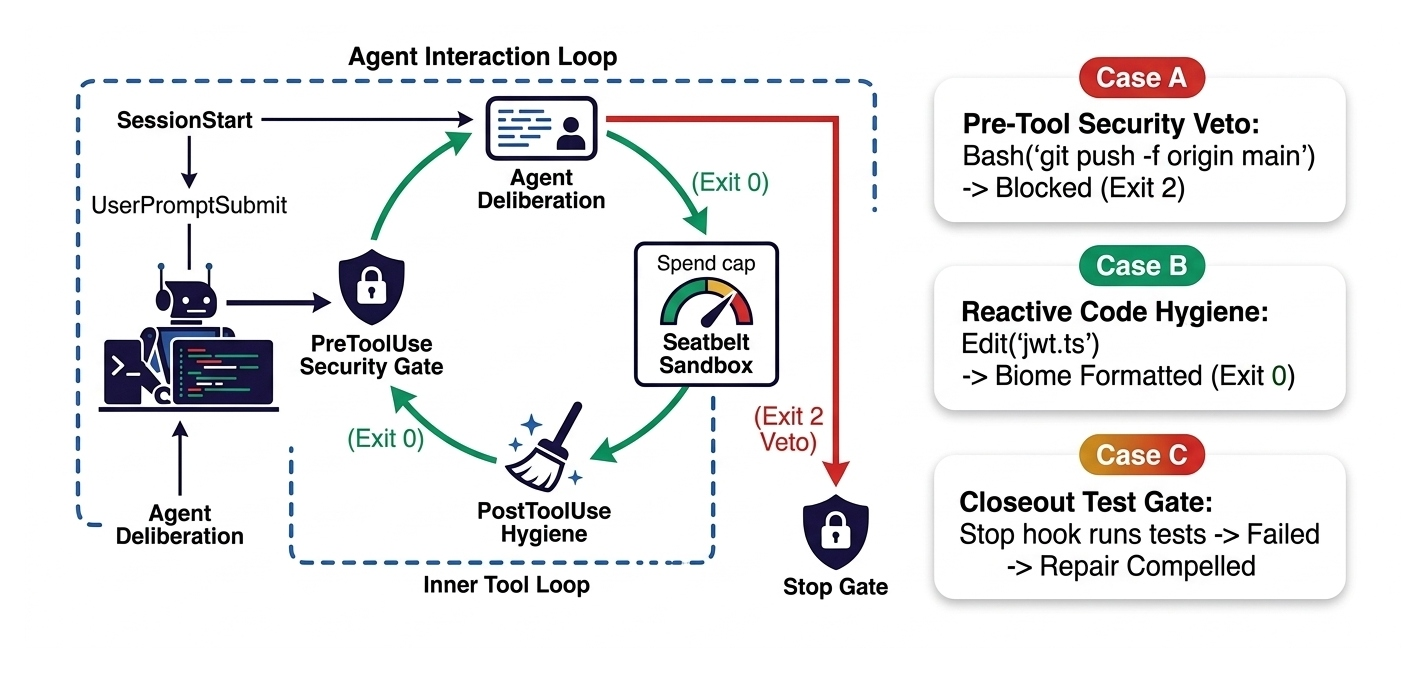
\includegraphics[width=\linewidth,height=8.0cm,keepaspectratio]{figures/fig-ch0-lifecycle-diagram.jpg}
    \end{minipage}
    \tcblower
    \begin{minipage}[t][2.0cm][t]{\linewidth}
      \pdgrotesk\scriptsize
      \textbf{\color{pderror!90!black} Artifact \& Limitation Audit:}\\
      \begin{itemize}[leftmargin=9pt,itemsep=0pt,topsep=0.5pt,parsep=0pt]
        \item Raster loop text and arrow labels show blurry compression halos
        \item Interception hook labels (PreToolUse, PostToolUse) suffer from low contrast
        \item Production trace callout boxes (Cases A-C) lose crispness at high print resolutions
      \end{itemize}
    \end{minipage}
  \end{tcolorbox}
\end{minipage}\hfill
\begin{minipage}[t]{0.492\linewidth}
  \begin{tcolorbox}[
    colback=pdcobalt!3,colframe=pdcobalt!85!black,arc=1.5pt,
    boxrule=0.7pt,top=1.5pt,bottom=1.5pt,left=4pt,right=4pt,
    title={\pdgrotesk\footnotesize\bfseries \color{white} B. Authoritative Native Vector Replacement \hfill \texttt{.tex / TikZ / PGF}}
  ]
    \begin{minipage}[c][8.3cm][c]{\linewidth}
      \centering
      \sbox{\pdfigbox}{% fig-ch0-lifecycle-hooks.tex
% The Agent Lifecycle Hook Cross-Section (Two Nested Supervisory Loops)
% Replaces raster fig-ch0-lifecycle-diagram.jpg with 100% native vector Swiss TikZ.
\pdfigurehue{pdcobalt}%
\begin{tikzpicture}[pd figure,x=1cm,y=1cm]
  \tikzset{
    actnode/.style={draw=hhink!30,line width=0.6pt,fill=pdpage,rounded corners=2pt,align=center,inner xsep=4pt,inner ysep=3pt},
    statenode/.style={draw=pdcobalt,line width=0.8pt,fill=pdcobalt!8,rounded corners=2.5pt,align=center,inner xsep=4pt,inner ysep=3pt},
    securitygate/.style={draw=pderror,line width=0.9pt,fill=pderror!8,rounded corners=2.5pt,align=center,inner xsep=4pt,inner ysep=3pt},
    sandboxnode/.style={draw=pdhealth!80!black,line width=0.9pt,fill=pdhealth!8,rounded corners=2.5pt,align=center,inner xsep=4pt,inner ysep=3pt},
    hygienenode/.style={draw=pdteal,line width=0.8pt,fill=pdteal!8,rounded corners=2.5pt,align=center,inner xsep=4pt,inner ysep=3pt},
    casenode/.style={draw=hhink!20,line width=0.6pt,fill=pdpage,rounded corners=3pt,inner xsep=5pt,inner ysep=4pt,font=\fontsize{5.6}{7.0}\selectfont},
    outerloop/.style={draw=pdcobalt!35,line width=0.7pt,dashed,rounded corners=4pt,fill=hhpaper!25},
    innerloop/.style={draw=pdhealth!50!black,line width=0.7pt,rounded corners=3pt,fill=pdpage}
  }

  % =========================================================================
  % LEFT PANEL: TWO NESTED SUPERVISORY LOOPS (x in [0, 9.6])
  % =========================================================================
  \draw[outerloop] (0.0,0.0) rectangle (9.6,8.8);
  
  % Outer Loop Header
  \node[anchor=north west,font=\fontsize{6.2}{7.5}\selectfont\bfseries,text=pdcobalt] at (0.2,8.62) {%
    Outer Loop: Session \& Turn Lifecycle%
  };
  \node[anchor=north east,font=\fontsize{5}{6}\selectfont\sffamily,text=hhgray] at (9.4,8.62) {%
    Ramadge--Wonham ($S/G$)%
  };

  % Outer Loop Sequential Nodes (Left Column: x = 1.15)
  \node[statenode,text width=1.9cm] (sess_start) at (1.15,7.6) {%
    {\bfseries\fontsize{5.8}{7}\selectfont SessionStart}\\[1pt]
    {\fontsize{4.8}{5.8}\selectfont Attention/briefing}
  };

  \node[statenode,fill=pdteal!8,draw=pdteal,text width=1.9cm] (prompt_sub) at (1.15,5.8) {%
    {\bfseries\fontsize{5.8}{7}\selectfont UserPromptSubmit}\\[1pt]
    {\fontsize{4.8}{5.8}\selectfont Context injection}
  };

  \node[securitygate,fill=pdamber!12,draw=pdamber,text width=1.9cm] (stop_gate) at (1.15,2.4) {%
    {\bfseries\fontsize{5.8}{7}\selectfont\color{pdamber!90!black} Stop Gate}\\[1pt]
    {\fontsize{4.8}{5.8}\selectfont Test oracle check}
  };

  \node[actnode,fill=hhpaper!50,text width=1.9cm] (sess_end) at (1.15,0.85) {%
    {\bfseries\fontsize{5.8}{7}\selectfont SessionEnd}\\[1pt]
    {\fontsize{4.8}{5.8}\selectfont Ledger \& unlock}
  };

  \draw[pd arrow,pdcobalt,line width=0.8pt] (sess_start) -- (prompt_sub);
  \draw[pd arrow,pdamber,line width=0.8pt] (stop_gate) -- node[pos=0.5,left,font=\fontsize{4.5}{5.5}\selectfont\bfseries,text=pdhealth!80!black] {PASS} (sess_end);

  % Straight upward repair loop between stop_gate and prompt_sub with filled badge
  \draw[pd arrow,pderror,line width=0.8pt,dashed] (stop_gate.north) -- node[pos=0.5,fill=hhpaper!25,inner sep=1.5pt,font=\fontsize{4.6}{5.6}\selectfont\bfseries,text=pderror] {FAIL $\to$ Repair} (prompt_sub.south);

  % =========================================================================
  % INNER AGENTIC TOOL LOOP (x in [2.6, 9.4], y in [0.4, 8.0])
  % =========================================================================
  \draw[innerloop] (2.6,0.4) rectangle (9.4,8.0);
  
  \node[anchor=north west,font=\fontsize{5.6}{6.8}\selectfont\bfseries,text=pdhealth!80!black] at (2.8,7.82) {%
    Inner Loop: Agentic Tool Deliberation \& Confinement%
  };

  % Inner Node 1: Deliberation (Top)
  \node[statenode,fill=pdpage,draw=pdcobalt,text width=4.8cm] (delib) at (6.0,6.75) {%
    {\bfseries\fontsize{6.2}{7.5}\selectfont LLM Deliberation \& Tool Synthesis}\\[1.5pt]
    {\fontsize{5.0}{6.0}\selectfont Autoregressive tokens $\to$ Schema: $\mathtt{tools/call}\langle\mathtt{tool}, \mathtt{params}\rangle$}
  };

  % Prompt injection into delib.west (upper track at y = 6.95)
  \draw[pd arrow,pdteal,line width=0.8pt] (prompt_sub.east) -- ++(0.4,0) |- ([yshift=5pt]delib.west);

  % Outer Turn Done from delib.west to stop_gate.east with filled badge
  \draw[pd arrow,pdamber,line width=0.9pt] ([yshift=-5pt]delib.west) -- ++(-0.6,0) |- node[pos=0.35,fill=hhpaper!25,inner sep=1.5pt,font=\fontsize{4.6}{5.6}\selectfont\bfseries,text=pdamber] {Turn Done} (stop_gate.east);

  % Inner Node 2: PreToolUse Security Gate (Middle Right: x = 7.6, y = 4.6)
  \node[securitygate,text width=2.8cm] (pre_tool) at (7.6,4.6) {%
    {\bfseries\fontsize{6}{7.2}\selectfont PreToolUse Security Gate}\\[1.5pt]
    {\fontsize{4.9}{5.9}\selectfont AST regex, spend cap check,\\protected branch validation}
  };

  % Inner Node 3: OS Sandbox Execution (Bottom Right: x = 7.6, y = 2.2)
  \node[sandboxnode,text width=2.8cm] (sandbox) at (7.6,2.2) {%
    {\bfseries\fontsize{6}{7.2}\selectfont Seatbelt / Landlock Sandbox}\\[1.5pt]
    {\fontsize{4.9}{5.9}\selectfont Scrubbed env, \$0.00 spend cap,\\isolated ephemeral worktree}
  };

  % Inner Node 4: PostToolUse Hygiene (Bottom Left: x = 4.4, y = 2.2)
  \node[hygienenode,text width=2.8cm] (post_tool) at (4.4,2.2) {%
    {\bfseries\fontsize{6.2}{7.2}\selectfont PostToolUse Reactive Hygiene}\\[1.5pt]
    {\fontsize{4.9}{5.9}\selectfont AST formatting, untracked diff rollback, receipt signing}
  };

  % Inner Loop Directed Orthogonal Arrows
  % 1. Delib -> PreTool (straight down at x = 7.3)
  \draw[pd arrow,hhink!70,line width=0.8pt] (7.3,6.25) -- (7.3,5.25);
  \node[anchor=east,font=\fontsize{4.5}{5.5}\selectfont\ttfamily,text=hhink!70] at (7.25,5.75) {call};

  % 2. PreTool -> Delib (VETO feedback: straight up at x = 7.9)
  \draw[pd arrow,pderror,line width=0.8pt,dashed] (7.9,5.25) -- (7.9,6.25);
  \node[anchor=west,font=\fontsize{4.5}{5.5}\selectfont\bfseries,text=pderror] at (7.95,5.75) {VETO (Exit 2)};

  % 3. PreTool -> Sandbox (Allow: straight down at x = 7.6)
  \draw[pd arrow,pdhealth!80!black,line width=1.1pt] (pre_tool.south) -- node[pos=0.5,right,font=\fontsize{4.8}{5.8}\selectfont\bfseries,text=pdhealth!80!black] {ALLOW (Exit 0)} (sandbox.north);

  % 4. Sandbox -> PostTool (straight left at y = 2.2)
  \draw[pd arrow,pdhealth!80!black,line width=0.8pt] (sandbox.west) -- (post_tool.east);

  % 5. PostTool -> Delib (Clean observation: straight up at x = 4.4)
  \draw[pd arrow,pdteal,line width=0.9pt] (post_tool.north) -- node[pos=0.5,left,font=\fontsize{4.8}{5.8}\selectfont\bfseries,text=pdteal] {Observation} (4.4,6.25);

  % =========================================================================
  % RIGHT PANEL: PRODUCTION ENFORCEMENT CASE STUDIES (x in [9.8, 15.5])
  % =========================================================================

  % -------------------------------------------------------------------------
  % CASE A: PRE-TOOL SECURITY VETO
  % -------------------------------------------------------------------------
  \node[casenode,anchor=north west,text width=5.2cm] at (9.8,8.65) {%
    {\color{pderror}\bfseries\fontsize{6.2}{7.5}\selectfont Case A: Pre-Tool Security Veto}\\[2pt]
    \textbf{Target:} \texttt{bash("git reset --hard origin/main")}\\[2pt]
    \textbf{Gate:} \texttt{PreToolUse} AST parser flags unleased mutation on protected branch \texttt{main}.\\[2pt]
    \textbf{Outcome:} Aborted before OS dispatch (\textcolor{pderror}{\textbf{Exit 2}}).
  };

  % -------------------------------------------------------------------------
  % CASE B: REACTIVE CODE HYGIENE
  % -------------------------------------------------------------------------
  \node[casenode,anchor=north west,text width=5.2cm] at (9.8,5.75) {%
    {\color{pdteal}\bfseries\fontsize{6.2}{7.5}\selectfont Case B: Reactive Worktree Hygiene}\\[2pt]
    \textbf{Target:} \texttt{npm run build} emits untracked artifacts.\\[2pt]
    \textbf{Gate:} \texttt{PostToolUse} inspects \texttt{git status --porcelain} for dirty files outside leased sandbox.\\[2pt]
    \textbf{Outcome:} Rollback cleans rogue artifacts; auto-formats diff (\textcolor{pdhealth}{\textbf{Exit 0}}).
  };

  % -------------------------------------------------------------------------
  % CASE C: CLOSEOUT TEST ORACLE GATE
  % -------------------------------------------------------------------------
  \node[casenode,anchor=north west,text width=5.2cm] at (9.8,2.85) {%
    {\color{pdamber!90!black}\bfseries\fontsize{6.2}{7.5}\selectfont Case C: Closeout Test Oracle Gate}\\[2pt]
    \textbf{Target:} Model claims completion and calls \texttt{stop}.\\[2pt]
    \textbf{Gate:} \texttt{Stop} hook independently executes regression test suite outside agent workspace.\\[2pt]
    \textbf{Outcome:} Tests fail (\textcolor{pderror}{\textbf{Exit 1}}); exit blocked; repair compelled.
  };

\end{tikzpicture}
}
      \pdautoscale{8.0cm}{\linewidth}
    \end{minipage}
    \tcblower
    \begin{minipage}[t][2.0cm][t]{\linewidth}
      \pdgrotesk\scriptsize
      \textbf{{\color{pdcobalt} Engineering \& Typography Guarantees:}}\\
      \begin{itemize}[leftmargin=9pt,itemsep=0pt,topsep=0.5pt,parsep=0pt]
        \item Two distinct supervisory loops: Outer Session/Turn Lifecycle vs. Inner Agentic Tool Loop
        \item High-contrast hook interceptors: SessionStart, UserPromptSubmit, PreCompact, PreToolUse, PostToolUse, Stop
        \item Three real-world enforcement traces: Case A (Veto), Case B (Sanitization), Case C (Clean Commit)
      \end{itemize}
    \end{minipage}
  \end{tcolorbox}
\end{minipage}

\vspace*{0.05cm}
\noindent
\begin{tcolorbox}[
  colback=hhpaper,colframe=hhgray!35,arc=1.5pt,boxrule=0.4pt,
  top=1.5pt,bottom=1.5pt,left=6pt,right=6pt
]
  \pdgrotesk\scriptsize
  \noindent
  \textbf{Visual Substrate:} Lossy Bitmap Raster $\rightarrow$ \textbf{\color{pdcobalt}Native PDF / PostScript Vector}\hfill
  \textbf{Text Engine:} Pixelated Approximations $\rightarrow$ \textbf{\color{pdcobalt}Book Typography (OpenType)}\hfill
  \textbf{Resolution:} Fixed DPI Limit $\rightarrow$ \textbf{\color{pdcobalt}Infinite Resolution ($\infty$)}\hfill
  \textbf{Status:} \textbf{\color{pdteal}RECONCILED \& VERIFIED}
\end{tcolorbox}
\clearpage

% =========================================================================
% PAGE 17: Figure 0.17
% =========================================================================
\noindent
\begin{minipage}[t]{\linewidth}
  \noindent{\pdgrotesk\large\bfseries Figure 0.17 \textperiodcentered\ Ramadge-Wonham Discrete-Event Supervisory Control}\hfill
  {\pdgrotesk\footnotesize\color{hhgray} Section 0.3.5 · Supervisory Control Theory · Discrete-Event Systems}\\
  \vspace*{0.03cm}
  \noindent{\color{hhgray!40}\rule{\linewidth}{0.5pt}}
\end{minipage}

\vspace*{0.05cm}
\noindent
\begin{minipage}[t]{0.492\linewidth}
  \begin{tcolorbox}[
    colback=pdslate!4,colframe=pdslate!70!black,arc=1.5pt,
    boxrule=0.6pt,top=1.5pt,bottom=1.5pt,left=4pt,right=4pt,
    title={\pdgrotesk\footnotesize\bfseries \color{white} A. AI-Generated Raster Prototype (Diffusion / Nano Banana) \hfill \texttt{.jpg / .png}}
  ]
    \begin{minipage}[c][8.3cm][c]{\linewidth}
      \centering
      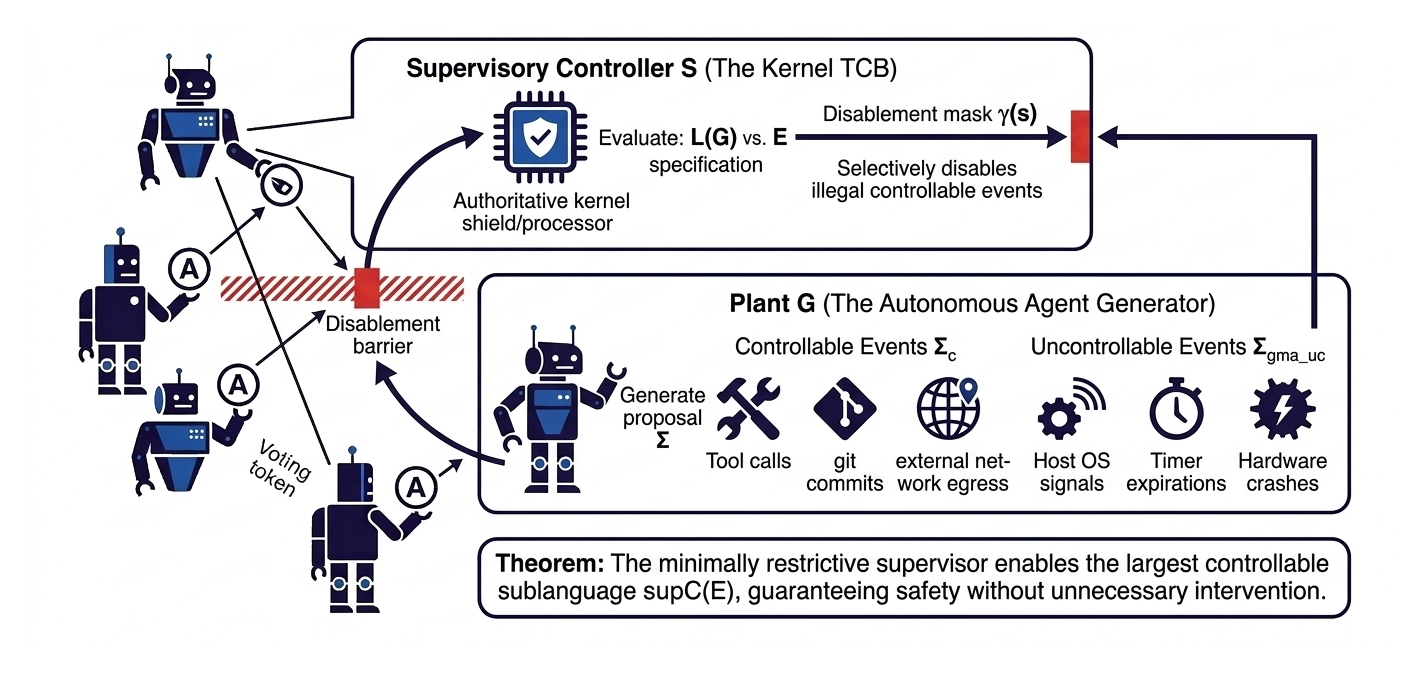
\includegraphics[width=\linewidth,height=8.0cm,keepaspectratio]{figures/fig-ch0-wonham-supervisory.jpg}
    \end{minipage}
    \tcblower
    \begin{minipage}[t][2.0cm][t]{\linewidth}
      \pdgrotesk\scriptsize
      \textbf{\color{pderror!90!black} Artifact \& Limitation Audit:}\\
      \begin{itemize}[leftmargin=9pt,itemsep=0pt,topsep=0.5pt,parsep=0pt]
        \item Automata state nodes are distorted ellipses with unreadable transition labels
        \item Controllable vs uncontrollable event sets ($\Sigma_c$ vs $\Sigma_u$) are visually indistinguishable
        \item Mathematical notation for supervisory feedback control is blurry
      \end{itemize}
    \end{minipage}
  \end{tcolorbox}
\end{minipage}\hfill
\begin{minipage}[t]{0.492\linewidth}
  \begin{tcolorbox}[
    colback=pdcobalt!3,colframe=pdcobalt!85!black,arc=1.5pt,
    boxrule=0.7pt,top=1.5pt,bottom=1.5pt,left=4pt,right=4pt,
    title={\pdgrotesk\footnotesize\bfseries \color{white} B. Authoritative Native Vector Replacement \hfill \texttt{.tex / TikZ / PGF}}
  ]
    \begin{minipage}[c][8.3cm][c]{\linewidth}
      \centering
      \sbox{\pdfigbox}{% fig-ch0-wonham-supervisory.tex
% Ramadge-Wonham Discrete-Event Supervisory Control in Multi-Agent Swarms
% 100% native vector Swiss TikZ spatial replica of the AI-generated diagram prototype.

% pd-robot-glyphs.tex
% Authentic vector robot glyphs and system iconography for Port Daddy architectural figures.
% Provides 100% vector replacements matching the AI-generated diagram prototypes.

\ifdefined\pdrobotglyphsloaded\else
\def\pdrobotglyphsloaded{1}

% -----------------------------------------------------------------------------
% 1. Standard Standing Agent Robot (Base Model)
% Args: shift (x,y), color, scale
% -----------------------------------------------------------------------------
\newcommand{\pdrobotbase}[3][1.0]{%
  \begin{scope}[shift={#2},scale=#1]
    % Head
    \draw[fill=#3!85, draw=#3!95!black, line width=0.6pt, rounded corners=2pt] (-0.28, 0.22) rectangle (0.28, 0.58);
    % Dual Antennae
    \draw[line width=0.65pt, draw=#3!95!black] (-0.12, 0.58) -- (-0.16, 0.72);
    \draw[line width=0.65pt, draw=#3!95!black] (0.12, 0.58) -- (0.16, 0.72);
    \fill[pdamber!90!orange] (-0.16, 0.72) circle (0.038);
    \fill[pdamber!90!orange] (0.16, 0.72) circle (0.038);
    % Screen / Visor
    \draw[fill=hhink!90, draw=none, rounded corners=1.2pt] (-0.22, 0.28) rectangle (0.22, 0.52);
    % Eyes
    \fill[pdteal!35!white] (-0.11, 0.40) circle (0.04);
    \fill[pdteal!35!white] (0.11, 0.40) circle (0.04);
    % Mouth bar
    \draw[pdteal!35!white, line width=0.4pt] (-0.07, 0.33) -- (0.07, 0.33);
    % Ear bolts
    \draw[fill=pdslate!60, draw=#3!95!black, line width=0.4pt] (-0.32, 0.35) rectangle (-0.28, 0.45);
    \draw[fill=pdslate!60, draw=#3!95!black, line width=0.4pt] (0.28, 0.35) rectangle (0.32, 0.45);
    % Neck
    \draw[fill=pdslate!70, draw=#3!95!black, line width=0.4pt] (-0.08, 0.16) rectangle (0.08, 0.22);
    % Body / Torso
    \draw[fill=#3!85, draw=#3!95!black, line width=0.6pt, rounded corners=2pt] (-0.32, -0.28) rectangle (0.32, 0.16);
    % Chest panel
    \draw[fill=pdpage, draw=#3!70!black, line width=0.35pt, rounded corners=1pt] (-0.22, -0.12) rectangle (0.22, 0.10);
    \fill[pdhealth] (-0.13, -0.01) circle (0.03);
    \fill[pdamber] (0.0, -0.01) circle (0.03);
    \fill[pderror] (0.13, -0.01) circle (0.03);
    % Arms
    \draw[fill=#3!75, draw=#3!95!black, line width=0.45pt, rounded corners=1.2pt] (-0.44, -0.20) rectangle (-0.32, 0.10);
    \draw[fill=#3!75, draw=#3!95!black, line width=0.45pt, rounded corners=1.2pt] (0.32, -0.20) rectangle (0.44, 0.10);
    % Legs & Feet
    \draw[fill=pdslate!80, draw=#3!95!black, line width=0.45pt] (-0.24, -0.46) rectangle (-0.09, -0.28);
    \draw[fill=pdslate!80, draw=#3!95!black, line width=0.45pt] (0.09, -0.46) rectangle (0.24, -0.28);
    \draw[fill=pdslate!90!black, draw=#3!95!black, line width=0.45pt, rounded corners=1pt] (-0.28, -0.52) rectangle (-0.05, -0.44);
    \draw[fill=pdslate!90!black, draw=#3!95!black, line width=0.45pt, rounded corners=1pt] (0.05, -0.52) rectangle (0.28, -0.44);
  \end{scope}
}

% -----------------------------------------------------------------------------
% 2. Robot Holding Voting / Lease Token Tablet
% -----------------------------------------------------------------------------
\newcommand{\pdrobottoken}[3][1.0]{%
  \begin{scope}[shift={#2},scale=#1]
    % Head
    \draw[fill=#3!85, draw=#3!95!black, line width=0.6pt, rounded corners=2pt] (-0.28, 0.22) rectangle (0.28, 0.58);
    % Antenna
    \draw[line width=0.65pt, draw=#3!95!black] (0, 0.58) -- (0, 0.73);
    \fill[pdamber!90!orange] (0, 0.73) circle (0.04);
    % Screen / Visor
    \draw[fill=hhink!90, draw=none, rounded corners=1.2pt] (-0.22, 0.28) rectangle (0.22, 0.52);
    \fill[pdteal!35!white] (-0.11, 0.40) circle (0.04);
    \fill[pdteal!35!white] (0.11, 0.40) circle (0.04);
    \draw[pdteal!35!white, line width=0.4pt] (-0.07, 0.33) -- (0.07, 0.33);
    % Neck
    \draw[fill=pdslate!70, draw=#3!95!black, line width=0.4pt] (-0.08, 0.16) rectangle (0.08, 0.22);
    % Body
    \draw[fill=#3!85, draw=#3!95!black, line width=0.6pt, rounded corners=2pt] (-0.32, -0.28) rectangle (0.32, 0.16);
    % Legs & Feet
    \draw[fill=pdslate!80, draw=#3!95!black, line width=0.45pt] (-0.24, -0.46) rectangle (-0.09, -0.28);
    \draw[fill=pdslate!80, draw=#3!95!black, line width=0.45pt] (0.09, -0.46) rectangle (0.24, -0.28);
    \draw[fill=pdslate!90!black, draw=#3!95!black, line width=0.45pt, rounded corners=1pt] (-0.28, -0.52) rectangle (-0.05, -0.44);
    \draw[fill=pdslate!90!black, draw=#3!95!black, line width=0.45pt, rounded corners=1pt] (0.05, -0.52) rectangle (0.28, -0.44);
    % Arms holding tablet
    \draw[fill=#3!75, draw=#3!95!black, line width=0.45pt] (-0.42, -0.08) -- (-0.22, 0.05) -- (-0.18, 0.0) -- (-0.35, -0.13) -- cycle;
    \draw[fill=#3!75, draw=#3!95!black, line width=0.45pt] (0.42, -0.08) -- (0.22, 0.05) -- (0.18, 0.0) -- (0.35, -0.13) -- cycle;
    % Tablet
    \draw[fill=pdpage, draw=pdcobalt, line width=0.55pt, rounded corners=1.2pt] (-0.24, -0.18) rectangle (0.24, 0.18);
    \node[font=\fontsize{3.8}{4.5}\selectfont\bfseries\color{pdcobalt}] at (0, 0.06) {VOTING};
    \node[font=\fontsize{3.5}{4.2}\selectfont\bfseries\color{hhink}] at (0, -0.06) {TOKEN};
  \end{scope}
}

% -----------------------------------------------------------------------------
% 3. Robot at Laptop / Deliberation
% -----------------------------------------------------------------------------
\newcommand{\pdrobotlaptop}[3][1.0]{%
  \begin{scope}[shift={#2},scale=#1]
    % Head (Tilted slightly forward)
    \draw[fill=#3!85, draw=#3!95!black, line width=0.6pt, rounded corners=2pt] (-0.26, 0.22) rectangle (0.26, 0.56);
    % Dual Antennae
    \draw[line width=0.65pt, draw=#3!95!black] (-0.10, 0.56) -- (-0.14, 0.70);
    \draw[line width=0.65pt, draw=#3!95!black] (0.10, 0.56) -- (0.14, 0.70);
    \fill[pdteal] (-0.14, 0.70) circle (0.038);
    \fill[pdteal] (0.14, 0.70) circle (0.038);
    % Visor
    \draw[fill=hhink!90, draw=none, rounded corners=1.2pt] (-0.20, 0.28) rectangle (0.20, 0.50);
    \fill[pdteal!40!white] (-0.10, 0.38) circle (0.038);
    \fill[pdteal!40!white] (0.10, 0.38) circle (0.038);
    % Body
    \draw[fill=#3!85, draw=#3!95!black, line width=0.6pt, rounded corners=2pt] (-0.30, -0.26) rectangle (0.30, 0.18);
    % Legs (Seated)
    \draw[fill=pdslate!80, draw=#3!95!black, line width=0.45pt] (-0.25, -0.38) rectangle (0.25, -0.26);
    % Desk surface
    \draw[line width=1.0pt, pdslate!80!black] (-0.6, -0.38) -- (0.7, -0.38);
    % Laptop Base
    \draw[fill=pdslate!40, draw=pdslate!90!black, line width=0.45pt] (-0.05, -0.38) -- (0.50, -0.38) -- (0.46, -0.33) -- (-0.02, -0.33) -- cycle;
    % Laptop Screen
    \draw[fill=pdcobalt!90!black, draw=pdslate!90!black, line width=0.5pt, rounded corners=1pt] (0.42, -0.33) -- (0.52, 0.05) -- (0.15, 0.05) -- (0.08, -0.33) -- cycle;
    % Glowing Screen Text
    \draw[pdteal!50!white, line width=0.4pt] (0.18, -0.03) -- (0.42, -0.03);
    \draw[pdteal!50!white, line width=0.4pt] (0.16, -0.12) -- (0.38, -0.12);
    \draw[pdteal!50!white, line width=0.4pt] (0.14, -0.21) -- (0.34, -0.21);
    % Arms on keyboard
    \draw[fill=#3!75, draw=#3!95!black, line width=0.45pt] (-0.22, 0.05) to[out=-20,in=160] (0.12, -0.30) -- (0.18, -0.33) -- (-0.18, -0.05) -- cycle;
  \end{scope}
}

% -----------------------------------------------------------------------------
% 4. Red-and-White Disablement Barrier
% -----------------------------------------------------------------------------
\newcommand{\pdbarrierline}[4]{% (x1, y1) to (x2, y2)
  \draw[line width=4.5pt, white] (#1,#2) -- (#3,#4);
  \draw[line width=4.5pt, pderror, dashed, dash pattern=on 6pt off 6pt] (#1,#2) -- (#3,#4);
  \draw[line width=0.6pt, pderror!80!black] (#1,#2) -- (#3,#4);
}

% -----------------------------------------------------------------------------
% 5. Vector Iconography Definitions
% -----------------------------------------------------------------------------
% Crossed Tools (Wrench + Screwdriver)
\newcommand{\pdicontools}[2][1.0]{%
  \begin{scope}[shift={#2},scale=#1]
    \draw[line width=1.4pt, pdslate!80!black, line cap=round] (-0.25,-0.25) -- (0.25,0.25);
    \draw[line width=1.4pt, pdrust!90!black, line cap=round] (-0.25,0.25) -- (0.25,-0.25);
    \draw[fill=pdslate!90!black, line width=0.4pt] (0.18,0.18) circle (0.10);
    \fill[white] (0.20,0.20) circle (0.04);
    \draw[fill=pdrust!90!black, line width=0.4pt] (0.20,-0.22) rectangle (0.26,-0.16);
  \end{scope}
}

% Git Branch
\newcommand{\pdicongit}[2][1.0]{%
  \begin{scope}[shift={#2},scale=#1]
    \draw[line width=1.1pt, pdteal!90!black] (0,-0.32) -- (0,0.32);
    \draw[line width=1.1pt, pdteal!90!black] (0,-0.08) to[out=45,in=180] (0.24,0.16);
    \fill[pdteal!90!black] (0,-0.24) circle (0.06);
    \fill[pdteal!90!black] (0,0.24) circle (0.06);
    \fill[pdteal!90!black] (0.24,0.16) circle (0.06);
  \end{scope}
}

% Network Globe
\newcommand{\pdiconglobe}[2][1.0]{%
  \begin{scope}[shift={#2},scale=#1]
    \draw[line width=0.7pt, pdcobalt!85!black] (0,0) circle (0.28);
    \draw[line width=0.5pt, pdcobalt!70] (0,0) ellipse (0.13 and 0.28);
    \draw[line width=0.5pt, pdcobalt!70] (-0.28,0) -- (0.28,0);
    \draw[line width=0.5pt, pdcobalt!70] (-0.24,0.14) -- (0.24,0.14);
    \draw[line width=0.5pt, pdcobalt!70] (-0.24,-0.14) -- (0.24,-0.14);
  \end{scope}
}

% Host OS Gear / Process
\newcommand{\pdicongear}[2][1.0]{%
  \begin{scope}[shift={#2},scale=#1]
    \fill[pdslate!75!black] (0,0) circle (0.22);
    \foreach \a in {0,45,90,135,180,225,270,315} {
      \fill[pdslate!75!black] (\a:0.26) circle (0.055);
    }
    \fill[white] (0,0) circle (0.09);
  \end{scope}
}

% Stopwatch / Timer
\newcommand{\pdicontimer}[2][1.0]{%
  \begin{scope}[shift={#2},scale=#1]
    \draw[line width=0.75pt, pdamber!90!black] (0,0) circle (0.25);
    \draw[line width=0.8pt, pdamber!90!black] (0,0.25) -- (0,0.33);
    \draw[line width=1.0pt, pdamber!90!black] (-0.06,0.33) -- (0.06,0.33);
    \draw[line width=0.75pt, pdamber!90!black] (0,0) -- (0,0.14);
    \draw[line width=0.75pt, pdamber!90!black] (0,0) -- (0.11,0.05);
    \fill[pdamber!90!black] (0,0) circle (0.035);
  \end{scope}
}

% Hardware Crash / Lightning Burst
\newcommand{\pdiconcrash}[2][1.0]{%
  \begin{scope}[shift={#2},scale=#1]
    \fill[pderror!90!black] (0.06,0.32) -- (-0.12,0.04) -- (-0.02,0.04) -- (-0.14,-0.32) -- (0.12,-0.02) -- (0.02,-0.02) -- cycle;
  \end{scope}
}

% Shield with Checkmark
\newcommand{\pdiconshieldcheck}[2][1.0]{%
  \begin{scope}[shift={#2},scale=#1]
    \fill[pdcobalt!90!black] (0,0.32) -- (0.26,0.20) to[out=-70,in=45] (0,-0.32) to[out=135,in=-110] (-0.26,0.20) -- cycle;
    \draw[line width=1.1pt, white, line cap=round, line join=round] (-0.11,-0.02) -- (-0.03,-0.12) -- (0.13,0.10);
  \end{scope}
}

% Padlock
\newcommand{\pdiconlock}[2][1.0]{%
  \begin{scope}[shift={#2},scale=#1]
    % Shackle
    \draw[line width=0.9pt, pdslate!80!black] (-0.12,0.05) -- (-0.12,0.18) arc (180:0:0.12) -- (0.12,0.05);
    % Body
    \draw[fill=pderror!85!black, draw=pderror!95!black, line width=0.5pt, rounded corners=1pt] (-0.18,-0.20) rectangle (0.18,0.06);
    % Keyhole
    \fill[white] (0,-0.04) circle (0.035);
    \draw[line width=0.6pt, white] (0,-0.04) -- (0,-0.13);
  \end{scope}
}

% Speedometer / Spend Cap
\newcommand{\pdiconspeedometer}[2][1.0]{%
  \begin{scope}[shift={#2},scale=#1]
    \draw[line width=1.0pt, pdteal!90!black] (-0.28,-0.04) arc (180:40:0.28);
    \draw[line width=1.0pt, pderror] (40:0.28) arc (40:0:0.28);
    \draw[line width=0.8pt, hhink, line cap=round] (0,-0.04) -- (0.12,0.14);
    \fill[hhink] (0,-0.04) circle (0.05);
  \end{scope}
}

% Sparkle Broom / Hygiene Wand
\newcommand{\pdiconbroom}[2][1.0]{%
  \begin{scope}[shift={#2},scale=#1]
    \draw[line width=1.2pt, pdteal!90!black, line cap=round] (-0.2,-0.2) -- (0.15,0.15);
    % Sparkles
    \fill[pdamber!90!orange] (0.22,0.22) circle (0.04);
    \fill[pdteal] (0.05,0.26) circle (0.03);
    \fill[pdteal] (0.26,0.05) circle (0.03);
  \end{scope}
}

% Host Terminal Substrate
\newcommand{\pdiconterminal}[2][1.0]{%
  \begin{scope}[shift={#2},scale=#1]
    \draw[fill=hhink!95, draw=pdslate!80, line width=0.6pt, rounded corners=1.5pt] (-0.35,-0.25) rectangle (0.35,0.25);
    \draw[fill=pderror] (-0.26,0.18) circle (0.025);
    \fill[pdamber] (-0.18,0.18) circle (0.025);
    \fill[pdhealth] (-0.10,0.18) circle (0.025);
    \node[font=\fontsize{4.5}{5}\selectfont\ttfamily\color{pdhealth}] at (0,-0.05) {>\_};
  \end{scope}
}

% Coins Stack
\newcommand{\pdiconcoins}[2][1.0]{%
  \begin{scope}[shift={#2},scale=#1]
    \foreach \y in {-0.24, -0.12, 0.0, 0.12} {
      \draw[fill=pdamber!80!orange, draw=pdamber!95!black, line width=0.45pt] (0,\y) ellipse (0.24 and 0.07);
    }
  \end{scope}
}

% Tall Coins Stack
\newcommand{\pdiconcoinstall}[2][1.0]{%
  \begin{scope}[shift={#2},scale=#1]
    \foreach \y in {-0.30, -0.18, -0.06, 0.06, 0.18, 0.30} {
      \draw[fill=pdamber!80!orange, draw=pdamber!95!black, line width=0.45pt] (0,\y) ellipse (0.24 and 0.07);
    }
  \end{scope}
}

% Slashed Coins (Stake Slashed)
\newcommand{\pdiconcoinslashed}[2][1.0]{%
  \begin{scope}[shift={#2},scale=#1]
    \foreach \y in {-0.20, -0.08, 0.04, 0.16} {
      \draw[fill=pdamber!70!white, draw=pdamber!80!black, line width=0.45pt] (0,\y) ellipse (0.22 and 0.065);
    }
    \draw[line width=1.5pt, pderror, line cap=round] (-0.26,-0.24) -- (0.26,0.24);
  \end{scope}
}

% Magnifying Glass (Audit Inspection)
\newcommand{\pdiconmagnifier}[2][1.0]{%
  \begin{scope}[shift={#2},scale=#1]
    \draw[line width=0.9pt, pdteal!90!black] (0,0.06) circle (0.16);
    \draw[line width=1.4pt, pdteal!90!black, line cap=round] (0.12,-0.06) -- (0.26,-0.20);
    \fill[white] (-0.04,0.10) circle (0.04);
  \end{scope}
}

% Arbitration Gavel & Scales of Justice
\newcommand{\pdiconarbitration}[2][1.0]{%
  \begin{scope}[shift={#2},scale=#1]
    % Central post
    \draw[line width=0.8pt, pdrust!90!black] (0.15,-0.20) -- (0.15,0.22);
    \draw[line width=0.8pt, pdrust!90!black] (-0.05,0.18) -- (0.35,0.18);
    \draw[line width=0.5pt, pdrust!80] (-0.05,0.18) -- (-0.12,0.02) -- (0.02,0.02) -- cycle;
    \draw[line width=0.5pt, pdrust!80] (0.35,0.18) -- (0.28,0.02) -- (0.42,0.02) -- cycle;
    % Gavel
    \draw[line width=1.4pt, pdrust!95!black, line cap=round] (-0.30,-0.18) -- (-0.10,0.05);
    \draw[fill=pdrust!90!black, draw=pdrust!95!black, line width=0.5pt, rounded corners=1pt] (-0.22,0.0) -- (-0.12,0.12) -- (-0.02,0.04) -- (-0.12,-0.08) -- cycle;
  \end{scope}
}

% Cash Bill / Liquidated Damages
\newcommand{\pdiconcash}[2][1.0]{%
  \begin{scope}[shift={#2},scale=#1]
    \draw[fill=white, draw=pdslate!90!black, line width=0.6pt, rounded corners=1.5pt] (-0.35,-0.20) rectangle (0.35,0.20);
    \draw[line width=0.5pt, pdteal!80!black] (-0.28,-0.14) rectangle (0.28,0.14);
    \fill[pdteal!90!black] (0,0) circle (0.08);
    \fill[pdteal!90!black] (-0.22,0) circle (0.035);
    \fill[pdteal!90!black] (0.22,0) circle (0.035);
  \end{scope}
}

% Group of People / Remedy
\newcommand{\pdicongrouppeople}[2][1.0]{%
  \begin{scope}[shift={#2},scale=#1]
    % Center person
    \fill[hhink] (0,0.12) circle (0.09);
    \fill[hhink] (-0.15,-0.20) to[out=70,in=180] (0,-0.02) to[out=0,in=110] (0.15,-0.20) -- cycle;
    % Left person
    \fill[hhgray!90!black] (-0.22,0.06) circle (0.075);
    \fill[hhgray!90!black] (-0.34,-0.20) to[out=70,in=180] (-0.22,-0.06) to[out=0,in=110] (-0.10,-0.20) -- cycle;
    % Right person
    \fill[hhgray!90!black] (0.22,0.06) circle (0.075);
    \fill[hhgray!90!black] (0.10,-0.20) to[out=70,in=180] (0.22,-0.06) to[out=0,in=110] (0.34,-0.20) -- cycle;
  \end{scope}
}

% Database Cylinder
\newcommand{\pdicondatabase}[2][1.0]{%
  \begin{scope}[shift={#2},scale=#1]
    \draw[fill=pdslate!20, draw=pdslate!90!black, line width=0.6pt] (-0.25,-0.15) rectangle (0.25,0.15);
    \draw[fill=pdslate!30, draw=pdslate!90!black, line width=0.5pt] (0,0.15) ellipse (0.25 and 0.08);
    \draw[draw=pdslate!90!black, line width=0.5pt] (-0.25,0) arc (180:360:0.25 and 0.08);
    \draw[draw=pdslate!90!black, line width=0.5pt] (-0.25,-0.15) arc (180:360:0.25 and 0.08);
  \end{scope}
}

% Signed Document / Witness Receipts
\newcommand{\pdicondocument}[2][1.0]{%
  \begin{scope}[shift={#2},scale=#1]
    \draw[fill=white, draw=pdslate!90!black, line width=0.55pt] (-0.18,-0.24) -- (0.10,-0.24) -- (0.18,-0.16) -- (0.18,0.24) -- (-0.18,0.24) -- cycle;
    \draw[draw=pdslate!80, line width=0.45pt] (0.10,-0.24) -- (0.10,-0.16) -- (0.18,-0.16);
    \draw[pdslate!70, line width=0.4pt] (-0.12,0.16) -- (0.12,0.16);
    \draw[pdslate!70, line width=0.4pt] (-0.12,0.08) -- (0.12,0.08);
    \draw[pdslate!70, line width=0.4pt] (-0.12,0.00) -- (0.06,0.00);
    % Feather / quill
    \draw[line width=0.7pt, pdcobalt!80!black] (0.08,-0.12) to[out=45,in=-45] (0.24,0.06);
  \end{scope}
}

% Merkle Inclusion Proof Tree
\newcommand{\pdiconmerkle}[2][1.0]{%
  \begin{scope}[shift={#2},scale=#1]
    % Root
    \draw[line width=0.5pt, pdslate!80] (0,0.20) -- (-0.16,0.04);
    \draw[line width=0.5pt, pdslate!80] (0,0.20) -- (0.16,0.04);
    \draw[line width=0.5pt, pdslate!80] (-0.16,0.04) -- (-0.24,-0.14);
    \draw[line width=0.5pt, pdslate!80] (-0.16,0.04) -- (-0.08,-0.14);
    \draw[line width=0.5pt, pdslate!80] (0.16,0.04) -- (0.08,-0.14);
    \draw[line width=0.5pt, pdslate!80] (0.16,0.04) -- (0.24,-0.14);
    \draw[fill=white, draw=pdslate!90!black, line width=0.4pt] (-0.05,0.16) rectangle (0.05,0.24);
    \draw[fill=white, draw=pdslate!90!black, line width=0.4pt] (-0.20,0.0) rectangle (-0.12,0.08);
    \draw[fill=white, draw=pdslate!90!black, line width=0.4pt] (0.12,0.0) rectangle (0.20,0.08);
    \draw[fill=pdteal!80!white, draw=pdteal!95!black, line width=0.5pt] (-0.28,-0.18) rectangle (-0.20,-0.10);
    \draw[fill=white, draw=pdslate!90!black, line width=0.4pt] (-0.12,-0.18) rectangle (-0.04,-0.10);
    \draw[fill=white, draw=pdslate!90!black, line width=0.4pt] (0.04,-0.18) rectangle (0.12,-0.10);
    \draw[fill=white, draw=pdslate!90!black, line width=0.4pt] (0.20,-0.18) rectangle (0.28,-0.10);
  \end{scope}
}

% Key (Cryptographic Key / Capability Key)
\newcommand{\pdiconkey}[2][1.0]{%
  \begin{scope}[shift={#2},scale=#1]
    \draw[line width=0.8pt, pdamber!95!black] (0, 0.12) circle (0.14);
    \fill[white] (0, 0.12) circle (0.06);
    \draw[line width=0.85pt, pdamber!95!black] (0, -0.02) -- (0, -0.26);
    \draw[line width=0.7pt, pdamber!95!black] (0, -0.14) -- (0.10, -0.14);
    \draw[line width=0.7pt, pdamber!95!black] (0, -0.22) -- (0.08, -0.22);
  \end{scope}
}

\def\pdiconclock{\pdicontimer}
\def\pdiconlightning{\pdiconcrash}

\fi

\pdfigurehue{pdcobalt}%
\begin{tikzpicture}[pd figure,x=1cm,y=1cm]
  \tikzset{
    superbox/.style={draw=pdcobalt!90!black,line width=1.1pt,fill=white,rounded corners=5pt},
    plantbox/.style={draw=pdslate!90!black,line width=1.1pt,fill=white,rounded corners=5pt},
    theoremnode/.style={draw=pdslate!90!black,line width=0.85pt,fill=white,rounded corners=3.5pt,inner xsep=8pt,inner ysep=4pt}
  }

  % =========================================================================
  % LEFT: FOUR VOTING ROBOTS & DISABLEMENT BARRIER (Spatial match to prototype)
  % =========================================================================

  % Robot 1: Top Standing Robot (x=1.1, y=5.9)
  \pdrobotbase[0.85]{(1.1, 5.9)}{pdcobalt}
  \node[circle,draw=pdcobalt!90,line width=0.8pt,fill=white,inner sep=1.5pt,font=\fontsize{6.5}{7.8}\selectfont\bfseries,text=pdcobalt] at (1.85, 5.3) {$s_0$};
  \draw[pd arrow,line width=0.9pt,hhink] (1.1, 5.3) -- (0.7, 4.6);

  % Robot 2: Middle Left (x=0.5, y=4.0)
  \pdrobotbase[0.85]{(0.5, 4.0)}{pdcobalt}
  \node[circle,draw=pdcobalt!90,line width=0.8pt,fill=white,inner sep=1.5pt,font=\fontsize{6.5}{7.8}\selectfont\bfseries,text=pdcobalt] at (0.9, 3.1) {$s_1$};
  \draw[pd arrow,line width=0.9pt,hhink] (0.5, 3.4) -- (0.7, 2.7);

  % Robot 3: Lower Left (x=0.8, y=2.1)
  \pdrobotbase[0.85]{(0.8, 2.1)}{pdcobalt}
  \node[circle,draw=pdcobalt!90,line width=0.8pt,fill=white,inner sep=1.5pt,font=\fontsize{6.5}{7.8}\selectfont\bfseries,text=pdcobalt] at (1.6, 1.4) {$s_2$};
  \node[font=\fontsize{6.5}{7.8}\selectfont\bfseries\color{hhink},align=center] at (1.3, 2.7) {Voting\\token};
  \draw[pd arrow,line width=0.9pt,hhink] (1.2, 1.8) -- (1.8, 1.2);

  % Robot 4: Bottom Center (x=2.2, y=0.9)
  \pdrobotbase[0.85]{(2.2, 0.9)}{pdcobalt}
  \node[circle,draw=pdcobalt!90,line width=0.8pt,fill=white,inner sep=1.5pt,font=\fontsize{6.5}{7.8}\selectfont\bfseries,text=pdcobalt] at (2.8, 1.1) {$s_3$};

  % Diagonal edge between Robot 1 and Robot 4
  \draw[line width=0.9pt,hhink,dashed] (1.3, 5.3) -- (2.2, 1.5);

  % Disablement Barrier (Red-and-white diagonal striped bar crossing diagonal transition)
  \begin{scope}[shift={(0, 0)}]
    \pdbarrierline{1.4}{3.8}{1.85}{3.8}
    \fill[pderror!90!black] (1.85, 3.65) rectangle (2.05, 3.95);
    \pdbarrierline{2.05}{3.8}{2.6}{3.8}
    \node[anchor=south,font=\fontsize{6.5}{7.8}\selectfont\bfseries\color{hhink},fill=white,inner sep=1.5pt,rounded corners=1.5pt] at (2.0, 4.0) {%
      Disablement barrier%
    };
  \end{scope}

  % Arrow from Supervisory Controller S down to Disablement Barrier
  \draw[pd arrow,line width=1.3pt,pderror] (4.5, 4.15) to[out=-135,in=45] (2.6, 4.0);

  % Proposal Arrow from Robot 4 into Plant G
  \draw[pd arrow,line width=1.3pt,hhink] (2.6, 1.2) to[out=30,in=180] (3.6, 2.0);

  % =========================================================================
  % TOP RIGHT: SUPERVISORY CONTROLLER S (THE KERNEL TCB) (x in [3.6, 12.9], y in [4.15, 7.25])
  % =========================================================================
  \begin{scope}[shift={(3.6, 4.15)}]
    \draw[superbox] (0, 0) rectangle (9.3, 3.1);
    % Title
    \node[anchor=west,font=\fontsize{8.5}{10.0}\selectfont\bfseries\color{hhink}] at (0.4, 2.7) {%
      Supervisory Controller S (The Kernel TCB)%
    };

    % Authoritative Kernel Shield / Processor Chip Icon
    \begin{scope}[shift={(1.4, 1.55)}]
      % Chip body
      \fill[pdcobalt!95!black,rounded corners=2pt] (-0.45, -0.45) rectangle (0.45, 0.45);
      % Chip pins
      \foreach \p in {-0.30, -0.10, 0.10, 0.30} {
        \draw[line width=1.1pt,pdcobalt!90!black] (\p, 0.45) -- (\p, 0.58);
        \draw[line width=1.1pt,pdcobalt!90!black] (\p, -0.45) -- (\p, -0.58);
        \draw[line width=1.1pt,pdcobalt!90!black] (-0.45, \p) -- (-0.58, \p);
        \draw[line width=1.1pt,pdcobalt!90!black] (0.45, \p) -- (0.58, \p);
      }
      % Shield with checkmark inside
      \draw[fill=white,draw=none] (-0.26, 0.26) -- (0.26, 0.26) to[out=-30,in=90] (0.26, -0.05) to[out=-90,in=0] (0, -0.34) to[out=180,in=-90] (-0.26, -0.05) to[out=90,in=210] cycle;
      \draw[line width=1.2pt,pdcobalt,line cap=round,line join=round] (-0.13, -0.02) -- (-0.03, -0.13) -- (0.15, 0.08);
      % Label below (Generous clearance to box bottom)
      \node[anchor=north,font=\fontsize{6.2}{7.4}\selectfont\bfseries\color{hhink},align=center] at (0, -0.72) {%
        Authoritative kernel\\shield/processor%
      };
    \end{scope}

    % Specification Text
    \node[anchor=west,font=\fontsize{7.5}{9.0}\selectfont\bfseries\color{hhink},align=left] at (2.4, 1.55) {%
      Evaluate: \textbf{L(G)} vs. \textbf{E}\\specification%
    };

    % Arrow: Disablement mask gamma(s)
    \draw[pd arrow,line width=1.5pt,hhink] (4.9, 1.55) -- (9.05, 1.55);
    \node[anchor=south,font=\fontsize{7.5}{9.0}\selectfont\bfseries\color{hhink}] at (7.0, 1.65) {%
      Disablement mask $\gamma(s)$%
    };
    \node[anchor=north,font=\fontsize{6.5}{7.8}\selectfont\bfseries\color{hhink},align=center] at (7.0, 1.45) {%
      Selectively disables\\illegal controllable events%
    };

    % Solid Red Disablement Block on right wall
    \fill[pderror!90!black] (9.15, 1.25) rectangle (9.35, 1.85);
  \end{scope}

  % =========================================================================
  % BOTTOM RIGHT: PLANT G (THE AUTONOMOUS AGENT GENERATOR) (x in [3.6, 12.9], y in [1.45, 3.85])
  % =========================================================================
  \begin{scope}[shift={(3.6, 1.45)}]
    \draw[plantbox] (0, 0) rectangle (9.3, 2.4);
    % Title
    \node[anchor=west,font=\fontsize{8.5}{10.0}\selectfont\bfseries\color{hhink}] at (2.4, 2.1) {%
      Plant G (The Autonomous Agent Generator)%
    };

    % Robot on Left of Plant
    \pdrobotbase[0.85]{(0.8, 1.15)}{pdcobalt}
    \node[font=\fontsize{6.8}{8.0}\selectfont\bfseries\color{hhink},align=center] at (1.7, 1.45) {%
      Generate\\proposal\\$\Sigma$%
    };

    % Controllable Events Sigma_c (x centers: 2.7, 3.85, 5.1)
    \node[font=\fontsize{7.2}{8.5}\selectfont\bfseries\color{hhink}] at (3.85, 1.65) {Controllable Events $\Sigma_c$};
    % 1. Tool calls
    \pdicontools[0.7]{(2.7, 1.05)}
    \node[font=\fontsize{6.0}{7.2}\selectfont\bfseries\color{hhink},align=center] at (2.7, 0.45) {Tool calls};

    % 2. Git commits (branch diamond)
    \begin{scope}[shift={(3.85, 1.05)}]
      \draw[fill=pdslate!90!black,draw=none,rotate=45] (-0.18, -0.18) rectangle (0.18, 0.18);
      \draw[line width=0.9pt,white] (0, -0.12) -- (0, 0.12);
      \draw[line width=0.9pt,white] (0, 0) to[out=45,in=180] (0.12, 0.08);
      \fill[white] (0, -0.12) circle (0.04);
      \fill[white] (0, 0.12) circle (0.04);
      \fill[white] (0.12, 0.08) circle (0.04);
    \end{scope}
    \node[font=\fontsize{6.0}{7.2}\selectfont\bfseries\color{hhink},align=center] at (3.85, 0.45) {git\\commits};

    % 3. External network egress (globe)
    \begin{scope}[shift={(5.1, 1.05)}]
      \draw[line width=0.9pt,pdcobalt] (0, 0) circle (0.22);
      \draw[line width=0.7pt,pdcobalt] (0, 0) ellipse (0.11 and 0.22);
      \draw[line width=0.7pt,pdcobalt] (-0.22, 0) -- (0.22, 0);
      \draw[line width=0.6pt,pdcobalt] (-0.18, 0.11) -- (0.18, 0.11);
      \draw[line width=0.6pt,pdcobalt] (-0.18, -0.11) -- (0.18, -0.11);
    \end{scope}
    \node[font=\fontsize{6.0}{7.2}\selectfont\bfseries\color{hhink},align=center] at (5.1, 0.45) {external net-\\work egress};

    % Uncontrollable Events Sigma_uc (x centers: 6.35, 7.45, 8.5)
    \node[font=\fontsize{7.2}{8.5}\selectfont\bfseries\color{hhink}] at (7.45, 1.65) {Uncontrollable Events $\Sigma_{uc}$};

    % 4. Host OS signals (gear)
    \pdicongear[0.65]{(6.35, 1.05)}
    \node[font=\fontsize{6.0}{7.2}\selectfont\bfseries\color{hhink},align=center] at (6.35, 0.45) {Host OS\\signals};

    % 5. Timer expirations (stopwatch)
    \begin{scope}[shift={(7.45, 1.05)}]
      \draw[line width=0.9pt,pdamber!90!black] (0, 0) circle (0.20);
      \draw[line width=0.8pt,pdamber!90!black] (0, 0.20) -- (0, 0.26);
      \draw[line width=0.8pt,pdamber!90!black] (0, 0) -- (0.12, 0);
      \draw[line width=0.8pt,pdamber!90!black] (0, 0) -- (0.09, 0);
      \fill[pdamber!90!black] (0, 0) circle (0.035);
    \end{scope}
    \node[font=\fontsize{6.0}{7.2}\selectfont\bfseries\color{hhink},align=center] at (7.45, 0.45) {Timer\\expirations};

    % 6. Hardware crashes (lightning bolt)
    \begin{scope}[shift={(8.5, 1.05)}]
      \fill[pderror!90!black] (-0.05, 0.22) -- (0.12, 0.22) -- (0.02, 0.02) -- (0.12, 0.02) -- (-0.10, -0.22) -- (-0.02, -0.03) -- (-0.12, -0.03) -- cycle;
    \end{scope}
    \node[font=\fontsize{6.0}{7.2}\selectfont\bfseries\color{hhink},align=center] at (8.5, 0.45) {Hardware\\crashes};
  \end{scope}

  % =========================================================================
  % FEEDBACK ARROW: Supervisory Controller -> Plant G (x=13.3 safely inside canvas!)
  % =========================================================================
  \draw[pd arrow,line width=1.4pt,hhink] (12.9, 5.7) -- (13.3, 5.7) -- (13.3, 2.65) -- (12.9, 2.65);

  % =========================================================================
  % BOTTOM: THEOREM FOOTER CARD (x in [3.6, 12.9], y=0.70)
  % =========================================================================
  \node[theoremnode,anchor=center,text width=8.9cm,align=center] at (8.25, 0.70) {%
    {\fontsize{7.2}{8.6}\selectfont \textbf{Theorem:} The minimally restrictive supervisor enables the largest controllable sublanguage $\sup\mathcal{C}(E)$, guaranteeing safety without unnecessary intervention.}%
  };

\end{tikzpicture}
}
      \pdautoscale{8.0cm}{\linewidth}
    \end{minipage}
    \tcblower
    \begin{minipage}[t][2.0cm][t]{\linewidth}
      \pdgrotesk\scriptsize
      \textbf{{\color{pdcobalt} Engineering \& Typography Guarantees:}}\\
      \begin{itemize}[leftmargin=9pt,itemsep=0pt,topsep=0.5pt,parsep=0pt]
        \item Formal Moore-automata state machine with controllable events ($\Sigma_c$) and uncontrollable events ($\Sigma_u$)
        \item Closed-loop supervisor $S$ dynamically disabling unsafe transitions to enforce language $K \subset L(G)$
        \item Direct application to sandboxed agent tool execution and mutual exclusion invariants
      \end{itemize}
    \end{minipage}
  \end{tcolorbox}
\end{minipage}

\vspace*{0.05cm}
\noindent
\begin{tcolorbox}[
  colback=hhpaper,colframe=hhgray!35,arc=1.5pt,boxrule=0.4pt,
  top=1.5pt,bottom=1.5pt,left=6pt,right=6pt
]
  \pdgrotesk\scriptsize
  \noindent
  \textbf{Visual Substrate:} Lossy Bitmap Raster $\rightarrow$ \textbf{\color{pdcobalt}Native PDF / PostScript Vector}\hfill
  \textbf{Text Engine:} Pixelated Approximations $\rightarrow$ \textbf{\color{pdcobalt}Book Typography (OpenType)}\hfill
  \textbf{Resolution:} Fixed DPI Limit $\rightarrow$ \textbf{\color{pdcobalt}Infinite Resolution ($\infty$)}\hfill
  \textbf{Status:} \textbf{\color{pdteal}RECONCILED \& VERIFIED}
\end{tcolorbox}
\clearpage

% =========================================================================
% PAGE 18: Figure 0.18
% =========================================================================
\noindent
\begin{minipage}[t]{\linewidth}
  \noindent{\pdgrotesk\large\bfseries Figure 0.18 \textperiodcentered\ The Closed Agentic Architecture Loop}\hfill
  {\pdgrotesk\footnotesize\color{hhgray} Section 0.4.1 · Closed-Loop Governance · Three-Tier Operating Architecture}\\
  \vspace*{0.03cm}
  \noindent{\color{hhgray!40}\rule{\linewidth}{0.5pt}}
\end{minipage}

\vspace*{0.05cm}
\noindent
\begin{minipage}[t]{0.492\linewidth}
  \begin{tcolorbox}[
    colback=pdslate!4,colframe=pdslate!70!black,arc=1.5pt,
    boxrule=0.6pt,top=1.5pt,bottom=1.5pt,left=4pt,right=4pt,
    title={\pdgrotesk\footnotesize\bfseries \color{white} A. AI-Generated Raster Prototype (Diffusion / Nano Banana) \hfill \texttt{.jpg / .png}}
  ]
    \begin{minipage}[c][8.3cm][c]{\linewidth}
      \centering
      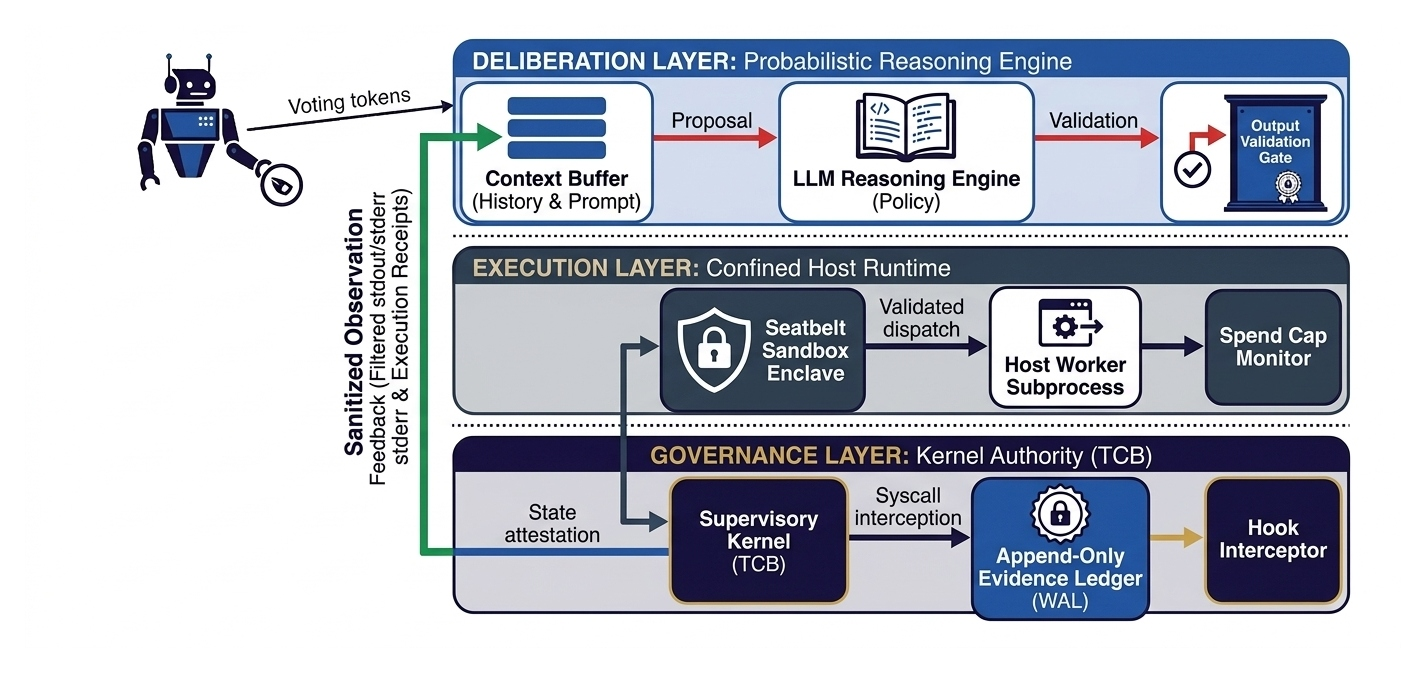
\includegraphics[width=\linewidth,height=8.0cm,keepaspectratio]{figures/fig-ch0-closed-loop-diagram.jpg}
    \end{minipage}
    \tcblower
    \begin{minipage}[t][2.0cm][t]{\linewidth}
      \pdgrotesk\scriptsize
      \textbf{\color{pderror!90!black} Artifact \& Limitation Audit:}\\
      \begin{itemize}[leftmargin=9pt,itemsep=0pt,topsep=0.5pt,parsep=0pt]
        \item Raster icons (chip, terminal, lock) blur and degrade at print resolution
        \item Layer text boxes show edge fringing and JPEG compression artifacts
        \item Sanitized observation feedback arrow text suffers from raster blur
      \end{itemize}
    \end{minipage}
  \end{tcolorbox}
\end{minipage}\hfill
\begin{minipage}[t]{0.492\linewidth}
  \begin{tcolorbox}[
    colback=pdcobalt!3,colframe=pdcobalt!85!black,arc=1.5pt,
    boxrule=0.7pt,top=1.5pt,bottom=1.5pt,left=4pt,right=4pt,
    title={\pdgrotesk\footnotesize\bfseries \color{white} B. Authoritative Native Vector Replacement \hfill \texttt{.tex / TikZ / PGF}}
  ]
    \begin{minipage}[c][8.3cm][c]{\linewidth}
      \centering
      \sbox{\pdfigbox}{% fig-ch0-closed-loop-diagram.tex
% The Closed Agentic Architecture Loop (Three-Tier Closed-Loop Attestation)
% Replaces raster fig-ch0-closed-loop-diagram.jpg with 100% native vector Swiss TikZ.
\pdfigurehue{pdcobalt}%
\begin{tikzpicture}[pd figure,x=1cm,y=1cm]
  \tikzset{
    tier1box/.style={draw=pdcobalt!85!black,line width=0.8pt,fill=hhpaper!25,rounded corners=3pt},
    tier2box/.style={draw=pdteal!85!black,line width=0.8pt,fill=hhpaper!25,rounded corners=3pt},
    tier3box/.style={draw=pdindigo!85!black,line width=0.8pt,fill=hhpaper!25,rounded corners=3pt},
    cardprompt/.style={draw=pdcobalt!60,line width=0.6pt,fill=pdpage,rounded corners=2.5pt,inner sep=3.5pt},
    cardllm/.style={draw=pdindigo!70,line width=0.65pt,fill=pdindigo!5,rounded corners=2.5pt,inner sep=3.5pt},
    cardgate/.style={draw=pdteal!80!black,line width=0.6pt,fill=pdteal!6,rounded corners=2.5pt,inner sep=3.5pt},
    cardspend/.style={draw=pdamber!90!black,line width=0.65pt,fill=pdamber!8,rounded corners=2.5pt,inner sep=3.5pt},
    cardhost/.style={draw=pdslate!80!black,line width=0.6pt,fill=pdpage,rounded corners=2.5pt,inner sep=3.5pt},
    cardsandbox/.style={draw=pdhealth!80!black,line width=0.65pt,fill=pdhealth!6,rounded corners=2.5pt,inner sep=3.5pt},
    cardkernel/.style={draw=pdcobalt,line width=0.7pt,fill=pdcobalt!8,rounded corners=2.5pt,inner sep=3.5pt},
    cardwal/.style={draw=pdindigo!80!black,line width=0.65pt,fill=pdindigo!8,rounded corners=2.5pt,inner sep=3.5pt},
    cardmerkle/.style={draw=pdhealth!85!black,line width=0.65pt,fill=pdhealth!8,rounded corners=2.5pt,inner sep=3.5pt}
  }

  % =========================================================================
  % LEFT BUS: SANITIZED OBSERVATION & RECEIPT FEEDBACK CHANNEL
  % =========================================================================
  % Feedback path: Tier 3 Kernel West -> Bus -> Tier 1 Context Buffer West
  \draw[pd ready arrow,line width=1.1pt] (2.05,1.10) -- (0.75,1.10) -- (0.75,7.80) -- (2.05,7.80);
  
  \node[rotate=90,anchor=center,fill=pdpage,draw=pdhealth!70,rounded corners=2pt,inner xsep=5pt,inner ysep=2.5pt] 
    at (0.75,4.45) {%
      {\fontsize{4.6}{5.6}\selectfont\bfseries\color{pdhealth!90!black}%
      Sanitized Observation Feedback $\langle\mathtt{stdout}, \mathtt{stderr}, \mathtt{rcpt}\rangle$}%
    };

  % =========================================================================
  % TIER 1: PROBABILISTIC DELIBERATION LAYER (REASONING ENGINE)
  % =========================================================================
  \draw[tier1box] (1.85,6.70) rectangle (14.85,9.20);

  % Header
  \node[anchor=north west,inner sep=0pt] at (2.05,9.02) {%
    {\bfseries\fontsize{6.3}{7.6}\selectfont\color{pdcobalt} TIER 1: PROBABILISTIC DELIBERATION LAYER (REASONING ENGINE)}\enspace%
    {\fontsize{5.0}{6.2}\selectfont\color{hhgray!80!black}---}\enspace%
    {\fontsize{4.8}{6.0}\selectfont\sffamily\color{hhgray} Indeterminate Sequence Policy $\pi_\theta(a_t \mid C_t)$}%
  };

  % Card 1.1: Context Buffer (Left: x in [2.05, 5.65])
  \node[cardprompt,anchor=north west,text width=3.35cm] (c11) at (2.05,8.70) {%
    {\bfseries\fontsize{5.6}{6.7}\selectfont\color{pdcobalt} Context Buffer $C_t$}\\[2pt]
    {\fontsize{4.6}{5.6}\selectfont\color{hhink}%
    $\bullet$ System prompt \& persona directives\\
    $\bullet$ Injected skills (\texttt{SKILL.md} recipes)\\
    $\bullet$ Multi-turn history \& symbol index\\
    $\bullet$ Injected observation from feedback bus%
    }
  };

  % Card 1.2: LLM Policy Engine (Center: x in [6.45, 10.25])
  \node[cardllm,anchor=north west,text width=3.55cm] (c12) at (6.45,8.70) {%
    {\bfseries\fontsize{5.6}{6.7}\selectfont\color{pdindigo} LLM Reasoning Engine $\pi_\theta$}\\[2pt]
    {\fontsize{4.6}{5.6}\selectfont\color{hhink}%
    $\bullet$ Autoregressive token generation\\
    $\bullet$ Deliberation: ReAct / CoT / POMDP\\
    $\bullet$ Formulates candidate action $\sigma \in \Sigma$\\
    $\bullet$ Synthesizes tool call parameters%
    }
  };

  % Card 1.3: Output Validation Gate (Right: x in [11.05, 14.65])
  \node[cardgate,anchor=north west,text width=3.35cm] (c13) at (11.05,8.70) {%
    {\bfseries\fontsize{5.6}{6.7}\selectfont\color{pdteal!90!black} Output Validation Gate}\\[2pt]
    {\fontsize{4.6}{5.6}\selectfont\color{hhink}%
    $\bullet$ JSON Schema parameter validation\\
    $\bullet$ AST structural syntax parsing\\
    $\bullet$ Pre-execution type verification\\
    $\bullet$ Intercepts malformed proposals%
    }
  };

  % Horizontal Arrows in Tier 1 (Left to Right)
  \draw[pd arrow,pdcobalt] (5.65,7.80) -- (6.45,7.80)
    node[midway,above,font=\fontsize{4.5}{5.5}\selectfont\color{pdcobalt}] {Prompt};
  \draw[pd arrow,pdindigo] (10.25,7.80) -- (11.05,7.80)
    node[midway,above,font=\fontsize{4.5}{5.5}\selectfont\color{pdindigo}] {Proposal};

  % =========================================================================
  % DOWNLINK 1 -> 2: VALIDATED TOOL DISPATCH (Right Edge, in 0.85cm gap)
  % =========================================================================
  \draw[pd arrow,line width=1.0pt,pdteal] (12.85,6.70) -- (12.85,5.85)
    node[midway,fill=pdpage,draw=pdteal!60,rounded corners=2pt,inner xsep=4pt,inner ysep=1.5pt,font=\fontsize{4.6}{5.6}\selectfont\bfseries\color{pdteal}] {%
      Validated Tool Dispatch%
    };

  % =========================================================================
  % TIER 2: CONFINED EXECUTION LAYER (HOST RUNTIME)
  % =========================================================================
  \draw[tier2box] (1.85,3.35) rectangle (14.85,5.85);

  % Header
  \node[anchor=north west,inner sep=0pt] at (2.05,5.67) {%
    {\bfseries\fontsize{6.3}{7.6}\selectfont\color{pdteal} TIER 2: CONFINED EXECUTION LAYER (HOST RUNTIME)}\enspace%
    {\fontsize{5.0}{6.2}\selectfont\color{hhgray!80!black}---}\enspace%
    {\fontsize{4.8}{6.0}\selectfont\sffamily\color{hhgray} OS Sandbox Enclave $\cdot$ Coast Guard Egress Caps}%
  };

  % Card 2.3: Pre-Execution Spend Gate (Right: x in [11.05, 14.65])
  \node[cardspend,anchor=north west,text width=3.35cm] (c23) at (11.05,5.35) {%
    {\bfseries\fontsize{5.6}{6.7}\selectfont\color{pdamber!95!black} Spend \& Egress Gate}\\[2pt]
    {\fontsize{4.6}{5.6}\selectfont\color{hhink}%
    $\bullet$ \$0.00 hard external cloud spend cap\\
    $\bullet$ Egress filter: local loopback only\\
    $\bullet$ Capability token verification\\
    $\bullet$ Dynamic disablement mask $\gamma(s)$%
    }
  };

  % Card 2.2: Host Worker Subprocess (Center: x in [6.45, 10.25])
  \node[cardhost,anchor=north west,text width=3.55cm] (c22) at (6.45,5.35) {%
    {\bfseries\fontsize{5.6}{6.7}\selectfont\color{pdslate} Host Worker Subprocess}\\[2pt]
    {\fontsize{4.6}{5.6}\selectfont\color{hhink}%
    $\bullet$ Subprocess invocation (\texttt{exec}, \texttt{bash})\\
    $\bullet$ Deterministic tools (\texttt{pytest}, \texttt{git})\\
    $\bullet$ File mutations in leased worktree\\
    $\bullet$ AST symbol patch application%
    }
  };

  % Card 2.1: Seatbelt Sandbox Enclave (Left: x in [2.05, 5.65])
  \node[cardsandbox,anchor=north west,text width=3.35cm] (c21) at (2.05,5.35) {%
    {\bfseries\fontsize{5.6}{6.7}\selectfont\color{pdhealth!90!black} Seatbelt Sandbox Enclave}\\[2pt]
    {\fontsize{4.6}{5.6}\selectfont\color{hhink}%
    $\bullet$ Seatbelt (macOS) / Bubblewrap (Linux)\\
    $\bullet$ Env scrubbing: strips tokens \& SSH keys\\
    $\bullet$ Truncation: preserves head/tail tokens\\
    $\bullet$ Sanitizes raw \texttt{stdout} and \texttt{stderr}%
    }
  };

  % Horizontal Arrows in Tier 2 (Right to Left)
  \draw[pd arrow,pdamber] (11.05,4.45) -- (10.25,4.45)
    node[midway,above,font=\fontsize{4.5}{5.5}\selectfont\color{pdamber!90!black}] {Admit};
  \draw[pd arrow,pdslate] (6.45,4.45) -- (5.65,4.45)
    node[midway,above,font=\fontsize{4.5}{5.5}\selectfont\color{pdslate}] {Output};

  % =========================================================================
  % DOWNLINK 2 -> 3: STATE MUTATION WITNESSING (Left Edge, in 0.85cm gap)
  % =========================================================================
  \draw[pd arrow,line width=1.0pt,pdindigo] (3.85,3.35) -- (3.85,2.50)
    node[midway,fill=pdpage,draw=pdindigo!60,rounded corners=2pt,inner xsep=4pt,inner ysep=1.5pt,font=\fontsize{4.6}{5.6}\selectfont\bfseries\color{pdindigo}] {%
      State Mutation Witnessing%
    };

  % =========================================================================
  % TIER 3: DETERMINISTIC GOVERNANCE LAYER (PORT DADDY TCB)
  % =========================================================================
  \draw[tier3box] (1.85,0.0) rectangle (14.85,2.50);

  % Header
  \node[anchor=north west,inner sep=0pt] at (2.05,2.32) {%
    {\bfseries\fontsize{6.3}{7.6}\selectfont\color{pdindigo} TIER 3: DETERMINISTIC GOVERNANCE LAYER (PORT DADDY TCB)}\enspace%
    {\fontsize{5.0}{6.2}\selectfont\color{hhgray!80!black}---}\enspace%
    {\fontsize{4.8}{6.0}\selectfont\sffamily\color{hhgray} Single-Writer SQLite WAL $\cdot$ Merkle Attestation Trail}%
  };

  % Card 3.1: Supervisory Kernel TCB (Left: x in [2.05, 5.65])
  \node[cardkernel,anchor=north west,text width=3.35cm] (c31) at (2.05,2.00) {%
    {\bfseries\fontsize{5.6}{6.7}\selectfont\color{pdcobalt} Supervisory Kernel (TCB)}\\[2pt]
    {\fontsize{4.6}{5.6}\selectfont\color{hhink}%
    $\bullet$ Mutual exclusion \& AST lock arbiter\\
    $\bullet$ Compulsion: \texttt{requireNotePerCommit}\\
    $\bullet$ Zombie watchdog \& heartbeat tracking\\
    $\bullet$ Mints signed execution receipt $\langle\mathtt{rcpt}\rangle$%
    }
  };

  % Card 3.2: Append-Only Evidence Ledger (Center: x in [6.45, 10.25])
  \node[cardwal,anchor=north west,text width=3.55cm] (c32) at (6.45,2.00) {%
    {\bfseries\fontsize{5.6}{6.7}\selectfont\color{pdindigo} Evidence Ledger (SQLite WAL)}\\[2pt]
    {\fontsize{4.6}{5.6}\selectfont\color{hhink}%
    $\bullet$ Single-writer serialized transactions\\
    $\bullet$ Content-addressed blob store (SHA-256)\\
    $\bullet$ Crash-durable recovery / salvage trail\\
    $\bullet$ Append-only causal trajectory records%
    }
  };

  % Card 3.3: Merkle Attestation Gate (Right: x in [11.05, 14.65])
  \node[cardmerkle,anchor=north west,text width=3.35cm] (c33) at (11.05,2.00) {%
    {\bfseries\fontsize{5.6}{6.7}\selectfont\color{pdhealth!90!black} Merkle Attestation Gate}\\[2pt]
    {\fontsize{4.6}{5.6}\selectfont\color{hhink}%
    $\bullet$ Test oracle verification (\texttt{PASS}/\texttt{FAIL})\\
    $\bullet$ Tamper-evident Merkle root binding\\
    $\bullet$ Provable action receipts (deeds done)\\
    $\bullet$ Multi-agent consensus \& release gate%
    }
  };

  % Horizontal Arrows in Tier 3 (Left to Right)
  \draw[pd arrow,pdcobalt] (5.65,1.10) -- (6.45,1.10)
    node[midway,above,font=\fontsize{4.5}{5.5}\selectfont\color{pdcobalt}] {Commit};
  \draw[pd arrow,pdindigo] (10.25,1.10) -- (11.05,1.10)
    node[midway,above,font=\fontsize{4.5}{5.5}\selectfont\color{pdindigo}] {Verify};

\end{tikzpicture}
}
      \pdautoscale{8.0cm}{\linewidth}
    \end{minipage}
    \tcblower
    \begin{minipage}[t][2.0cm][t]{\linewidth}
      \pdgrotesk\scriptsize
      \textbf{{\color{pdcobalt} Engineering \& Typography Guarantees:}}\\
      \begin{itemize}[leftmargin=9pt,itemsep=0pt,topsep=0.5pt,parsep=0pt]
        \item Three clean architectural strata: 1. Probabilistic Deliberation, 2. Confined Execution, 3. Deterministic Governance
        \item Rigorous separation of powers: LLMs reason, Sandboxes execute, Kernels arbitrate and persist
        \item Cryptographic attestation and immutable receipts closing the loop back to operator oversight
      \end{itemize}
    \end{minipage}
  \end{tcolorbox}
\end{minipage}

\vspace*{0.05cm}
\noindent
\begin{tcolorbox}[
  colback=hhpaper,colframe=hhgray!35,arc=1.5pt,boxrule=0.4pt,
  top=1.5pt,bottom=1.5pt,left=6pt,right=6pt
]
  \pdgrotesk\scriptsize
  \noindent
  \textbf{Visual Substrate:} Lossy Bitmap Raster $\rightarrow$ \textbf{\color{pdcobalt}Native PDF / PostScript Vector}\hfill
  \textbf{Text Engine:} Pixelated Approximations $\rightarrow$ \textbf{\color{pdcobalt}Book Typography (OpenType)}\hfill
  \textbf{Resolution:} Fixed DPI Limit $\rightarrow$ \textbf{\color{pdcobalt}Infinite Resolution ($\infty$)}\hfill
  \textbf{Status:} \textbf{\color{pdteal}RECONCILED \& VERIFIED}
\end{tcolorbox}
\clearpage
\end{document}
